%This seems to be the up-to-date version

\documentclass[a4,10pt]{book}
%\documentclass[a4,10pt]{article}
%\usepackage{arevmath}
\usepackage{amssymb}
 \usepackage{amsbsy}
 \usepackage{amsmath}
 \usepackage[english]{babel}
 \usepackage{bussproofs}
 \usepackage{boxedminipage}
 \usepackage{latexsym}
 \usepackage{graphicx}
 \usepackage{makeidx}
 \usepackage{lscape}
\usepackage{hyperref}
\usepackage{wasysym}
\usepackage{pifont}
\usepackage{latexsym}
\usepackage{graphicx}
\usepackage{epsfig}
\usepackage{pgf}
\usepackage{tikz}
\usepackage{color}
\usepackage{setspace}
\usetikzlibrary{arrows,automata}
\usepackage[latin1]{inputenc}
\usepackage{dingbat}
%\usepackage[utf8]{inputenc}
%\usepackage{pgf,tikz}
\usetikzlibrary{arrows}

\input newlogicmacr
%\renewcommand{\twoheadrightarrow}{\to\kern-7.5pt\to}
%\newcommand{\ZZ}{\hbox{\rm Z\kern-7.5pt Z}} 
\renewcommand{\N}{\mathfrak N}
\renewcommand{\i}{{\mathfrak i}} 
\newcommand{\setlike}{{\mathfrak S}{\mathfrak e}{\mathfrak t}{\mathfrak l}{{\i}}{\mathfrak k}{\mathfrak e}}
\newcommand{\doublecomp}{\sim\sim}

\newcommand{\internal}{{\mathfrak I}{\mathfrak n}{\mathfrak t}{\mathfrak e}{\mathfrak r}{\mathfrak n}{\mathfrak a}{\mathfrak l}}

\title{Scrapbook on Set Theory with a Universal Set}
\author{Thomas Forster}
\begin{document}

\maketitle

\sloppy
\tableofcontents
\vfill

\chapter{Stuff to fit in somewhere}

Ivan Vorobiev {\tt <ivanexplay2000@gmail.com>} writes on 5/vii/24 \ldots

\smallskip

There is some result that made me think about TC$_2$T again, namely
the paper ``Periodicity in the cumulative hierarchy" by Gabriel
Goldberg and Farmer Schlutzenberg: \url{https://arxiv.org/abs/2006.01103}.
In this paper they demonstrate the 2-periodicity of the high floors of
the cumulative hierarchy in the absence of the axiom of choice in the
presence of a Reinhardt cardinal in ZF. It became interesting, if we
take ${\cal P}^n(V_\alpha)$ as a model for TST, where $\alpha$ is the
Reinhardt cardinal and choose only 2-stratified formulas about it,
what would be the result?  As before, the question is motivated by the
fact that one wants to study ``small" and ``large" sets in the same
way. And as seen in ``Categories with New Foundations" NF handles this
not badly, but it seems that [reinforcements of] TC$_2$T can give a
more comprehensive picture.


\bigskip




The more i think about it, the odder the proof of AxInf looks.  We
have the principle that The Attic tells us nothing about wellfounded
sets.  So The Attic isn't going to tell us that there are infinite
wellfounded sets.  But it does tell us that there are infinite (small)
sets.

\bigskip

In Randall's models the power set of a wellorderable set is
wellorderable.  So the set of wellorderable sets is a fat set, so
every wellfounded set is wellorderable.



\bigskip

Zachiri sez that $\Pi_n$ collection plus $\Pi_{n+1}$ foundation implies $\Sigma_{n+1}$ separation.


\bigskip

I have been thinking about a construction of Crabb\'e's that Randall
showed me. Crabb\'e shows how to interpret NFU in SF.  This is like
the CUS situation in the following sense:
\begin{quote}
   We have a theory $T_1$ and a construction ${\cal C}$ which, whenever it is applied 
   to a model of $T_1$, gives a model of $T_2$.  We seek {\sl Beschr\"ankheitsaxiome} 
   ${\cal B}$ to add to $T_2$ so that $T_1$ and $T_2 + {\cal B}$ are synonymous.
\end{quote}
Can this always be done?  Tim has managed to do it where $T_1$ is ZF
(or anything like it) and $T_2$ is CUS (or something like it). My guess
would be that it requires special conditions.  Can we say anything about
what those special conditions are?  In particular what happens if $T_1$
is SF and ${\cal C}$ is Crabb\'e's construction?

Randall sez: Crabb\'e's construction probably doesn't witness synonymy
because it destroys information.  Objects which are coextensional
in SF are simply identified in NFU, and the information about the
extensions of objects in SF whose extensions are not unions of
equivalence classes under coextensionality is lost.

\bigskip

\bigskip

Is it always possible to expand a model of TST$_4$ to a model of TTT$_4$?
Randall sez no.  In contrast it is always possible to expand a (countable)
model of TST$_3$ to a model of TTT$_3$ -- Grischinology.  (There may be a
connection here with Pabion's work).  There is probably a set $\Sigma$ of
first-order sentences in ${\cal L}(TST_4)$ that one can add to TST$_4$ to
get a theory all of whose countable models can be expanded to a model of
TTT$_4$.  Randall sez that $\Sigma$ isn't as strong as NF and nor is he
putting any money on its refuting AC.



\bigskip


Zuhair has this idea for a different stratification algorithm.  The
idea, as usual, is to decorate every variable with a natural number.
You give all occurrences of any one variable to same natural number
of course.  And if you find the subformula $x=y$ you decorate `$x$'
and `$y$' with the same natural number. The difference comes with
$x \in y$. If you have decorated `$x$' but not `$y$' you give `$y$'
a decoration that is bigger than the decoration given to `$x$' \ldots
and analogously if you have decorated `$y$' but not yet `$x$'.

He posts this in
\url{https://mathoverflow.net/questions/437961/is-stratified-sorted-rendering-of-naive-set-theory-equivalent-to-tangled-type-th} Zuhair thinks it is something to do with Tangled type theory but
it's nothing of the sort; it clearly identifies as stratifiable
exactly the same sentences as were identified as stratifiable under
the old regime.



\section{A question for Randall}

Consider the following restriction/fragment of TTT.  Suppose (to keep
things simple) your levels are indexed by Z, the integers. You have a
relation $\in_{i,j}$ whenever $j = i+1$ or $i+2$, but no others. (Plus
the usual conditions that the extracted models are moels of TZT etc
etc.

One can also consider the weakening which has $\in_{i, j}$ where $j$
is $i+1$. $i+2$ or $i+3$.  And so on.


Randall sez that skipping one type is as good as skipping lots.

One wonders what happens constructively.

\bigskip

A conversation with Randall 27/xii/23

Randall, too, has noticed that the indices that decorate variables in
TZT aren't numbers. cf stratificationmodn.
We need to find the correct things to say about this.

Randall sez: take the one-sorted version of set theory.  Add a
predicate that says ``the equivalence class of $y$ is higher than the
equivalence class of $x$'' and axioms to say it is a strict order.  That
way you can prove that it has no loops.  This makes the theory finax!


Think about how to expunge unstratified separation in the one-sorted version of type theory.






\bigskip


Somewhere in these notes i point out that there is a choice function
on the set of cofinite sets.  But there can't be a choice sunction on
$|V|$.

\bigskip

$\{y \in x: y \not\in y\} \not\in x$.  Now substitute $(V\setminus x)/x]$

  $\{y \in (V\setminus x): y \not\in y\} \not\in (V \setminus x)$.  In other words:

  $\{y \not\in x: y \not\in y\} \in x$.  Or

      $\{y: y \not\in (x \cup y)\} \in x$.  

  But this is a global choice function!

  It might help to see a proof in \naive\ set theory.

  
  Can we use this to get a global choice function on $V_\omega$?  

  $\{y \in x: y \not\in y\} \not\in x$.  Now substitute $(V_\omega \setminus x)/x]$

    $\{y \in (V_\omega \setminus x): y \not\in y\} \not\in (V_\omega \setminus x)$.


    $\{y \in (V_\omega \setminus x): y \not\in y\} \not\in (V_\omega \setminus x)$.

    All this shows is that     $\{y \in (V_\omega \setminus x): y \not\in y\} \not\in V_\omega$.
    
\bigskip

Randall points out that in NFU you can't identify atoms with Quine atoms beco's of Cantor's theorem.
There are fewer Quine atoms than sets beco's of Cantor's theorem

Which subsystems of NF give easy relative consistency of duality?

Prove NF$_3$ is not finitely axiomatisable.

\section{An article on matters arising from the third edition?}

pseudo.tex;  pairsntuff.tex; SCU; axiom of infinity and Amb(arith)



\bigskip
small-scale open problems.  Does parameter-free NF prove infinity?

\bigskip

Notice that the set $NO$ does not have an easy inductive definition.
It's a quotient of an inductively defined set but isn't easily
inductively defined itself.

\section{Specker's refutation of AC: does it need parameters?}

\url{https://us.metamath.org/nfeuni/nchoice.html} provides a proof, and cites the following axioms:
\begin{tabbing}
  {\tt  ax-1}  \,\,\,\,\,\,\,\,\,\,\,\,\,\,\,\,\,\,\,\,\,\,\,\,\,\,\,\,\,\,  \=5,\\
{\tt ax-2}}                     \> 7,\\
{\tt ax-mp}                     \> 8,\\
{\tt ax-meredith}               \> 1406\\
{\tt ax-gen}                    \> 1546,\\
{\tt ax-5}                      \> 1557,\\
{\tt ax-17}                     \> 1616,\\
{\tt ax-9}                      \> 1654,\\
{\tt ax-8 }                      \> 1675,\\
{\tt ax-13}                      \> 1712,\\
{\tt ax-14}                      \> 1714,\\    
{\tt ax-6 }                      \> 1729,\\
{\tt ax-7 }                      \> 1734,\\
{\tt ax-11}                      \> 1746,\\
{\tt ax-12}                      \> 1925,\\
{\tt ax-ext}                     \> 2334,\\
{\tt ax-nin}                     \> 4078,\\
{\tt ax-xp}                      \> 4079,\\
{\tt ax-cnv}                     \> 4080,\\
{\tt ax-1c}                      \> 4081,\\
{\tt ax-sset}                    \> 4082,\\
{\tt ax-si}                     \> 4083,\\
{\tt ax-ins2}                   \> 4084,\\
{\tt ax-ins3}                   \> 4085,\\
{\tt ax-typlower}               \> 4086,\\
{\tt ax-sn}                     \> 4087.
\end{tabbing}
That's 27 axioms. I assume that the numbers in the second column are line numbers.

Everything in the list before {\tt ax-ext} is a logical axiom.

{\tt ax-ext} is the axiom of extensionality.

{\tt ax-nin} is the axiom that give $\overline{x \cap y}$.
  It is of course \textcolor{red}{not} an axiom of NFpf

{\tt ax-xp} gives cartesian products; it is \textcolor{red}{not} an axiom of NFpf;

{\tt ax-cnv} gives converses of relation; it is \textcolor{red}{not} an axiom of NFpf;

{\tt ax-1c} gives the set of all singletons; it is an axiom of NFpf;

{\tt ax-sset} gives the graph of $\subseteq$; it is an axiom of NFpf;

{\tt ax-si} is Hailperin's axiom P2; it is \textcolor{red}{not} an axiom of NFpf;

{\tt ax-ins2} is Hailperin's axiom P3; it is \textcolor{red}{not} an axiom of NFpf;

{\tt ax-ins3} is Hailperin's axiom P4; it is \textcolor{red}{not} an axiom of NFpf;

{\tt ax-typlower} is Hailperin's axiom P6; it is \textcolor{red}{not} an axiom of NFpf;

{\tt ax-sn} asserts the existence of a singleton; it is an axiom of NFpf.

The axioms we need to worry about are flagged by red 

\section{A cunning plan to prove Con({\sl i}NF)}

\newcommand{\isf}{{\sl i}SF$^{pf}$}

Just had a bright idea.  Extensionality is what makes life difficult,
buggers up the proof theory.  SF is NF without extensionality, and
it's obviously consistent. Does it have a term model? {\sl The point
  is that a term model for SF is perforce a model of NF: you get
  extensionality free!}  Indeed a term model for the {\sl
  parameter-free} version of SF is a model for NF!  Another thing that
makes proof theory more tractable is restricting ourselves to a
constructive logic.  Restricting ourselves thus means that we are
looking for a consistency proof for {\sl i}NF rather than NF, and that
may well be a weaker result so we might be able to get something
without strong assumptions. So let us consider the constructive
parameter-free fragment of SF, which we will call \isf. It will
have very nice proof theory. In fact i'm banking on it having
cut-elimination, by work of Crabb\'e. Can we use this nice proof
theory to show that it has a term model?

So \isf is a theory in the language of set theory enriched with
term-forming apparatus: `$\{x:\phi\}$' is a term whenever $\phi(x)$
is stratified and has no free variables other than `$x$'.  It has
the usual rules for constructive first-order predicate logic, plus
$\in$-int and $\in$-elim for stratified parameter-free expressions:
$$\frac{\phi(x)}{x \in \{y: \phi(y)\}} \quad \frac{x \in \{y: \phi(y)\}}{\phi(x)}$$
where $\phi$ is stratified and has no parameters.   Actually i have
rather got into the habit of using a sequent presentation, so i will
use instead the two rules of $\in$-L and $\in$-R (wot i got from
Marcel's slides):

$$\frac{\Gamma \phi(x)\vdash \Delta}{\Gamma, x \in \{y: \phi(y)\}\vdash \Delta} \quad \frac{\Gamma \vdash \phi(x)}{\Gamma \vdash  x \in \{y: \phi(y)\}}$$

We will need to establish that \isf has the existence property.
If we haven't got that we are completely stymied.  Cut-elimination, and so on.

The plan is to show that \isf has a term model, and that that
term model is a model of {\sl i}NF.  If we then think of that term
model as a Kripke model it appears that the carrier set of each
component world in the Kripke model will simply be the set of closed
stratified set abstracts, so we will presumably get not just a model
of \isf but of \isf + CD, the constant domain axiom. Each world will
correspond to an extension of \isf, and it will believe an atomic
$s=t$ or $s \in t$ iff that is a theorem of the corresponding theory.
We hope that the theories corresponding to worlds in this way all
have the disjunction property!

The way to do this is to show that \isf can be extended to a theory
that locally omits the $1-$type that says that $x$ is not the
denotation of a closed set abstract.  This will involve getting
straight quite what form omitting types takes in a constructive
context.


Let $\phi$ be some property s.t. \isf proves that $\phi(x) \to$
``$x$ is not the denotation of a closed stratified set abstract''.
That is to say, for each stratified set abstract $t$, \isf
$\vdash (\forall x)(\phi(x) \to x \not= t)$. (Let us say such a
$\phi$ is {\sl bad}).

It will be quite useful in what follows that every bad $\phi$ is
equivalent to something unstratified that is bad:
$\phi(x) \bic (\phi(x) \wedge \neg\neg (x \in x \vee \neg(x\in x)))$

Notice that, for each theory $T$, the set of one-place predicates
that $T$ believes to be bad is closed under disjunction.  We want to
be able to consistently add $\neg\exists x\phi(x)$ for all bad $\phi$.
These are the {\sl badness avoidance axioms}. The fact that bad
predicates are closed under disjunction means that to prove the
simultaneous consistency of all the badness avoidance axioms for $T$
it is enuff to prove the consistency of each one.

That means that we have to establish that
\isf $\not\vdash \neg\neg\exists x \phi(x)$. 

The way to do this is by reasoning about proofs in \isf.

Let's start with the---presumably easier---claim that \isf
$\not\vdash \exists x \phi(x)$.  It's a rehearsal, and if
it doesn't work then we know not to try to establish \isf
$\not\vdash \neg\neg\exists x \phi(x)$.  

This would be straightforward were it not for the availability of the
$\in$-rules, and it is indeed straightforward for any unstratified
$\phi$.  For stratified $\phi$ the problem is that any stratified
expression with a free variable in it will match the output of
$\in$-elim.  But we can at least bank the fact that if $\phi$ is
unstratified or has no embedded terms then $\exists x \phi(x)$ doesn't
match the output of $\in$-elim, and can only have come from
$\exists$-R---which is of course impossible.   Fortunately every bad
predicate is equivalent to an unstratified bad predicate.

So we need to consider the cases where $\phi$ is stratified and has embedded terms.

We will need the concept of a {\sl reduced} expression.  This will be
one wherein all occurences of `$x \in \{y: \theta(y)\}$' have been
replaced by `$\theta(x)$'.  This will ensure that no closed set abstract
appears to the right of an `$\in$'.  We must check that the process of
rewriting that this appeals to is terminating and confluent.
(Termination matters, confluence perhaps not so much) \Wlog\ we may
assume all expressions are reduced.

Now consider the equivalence relation on (denotations of) stratified
closed parameter-free set abstracts of belonging to the same things.
This supports a rule of substitution.  Suppose $s$ and $t$ are
(denotations of) stratified closed parameter-free set abstracts that
belong to the same things.  Consider $\phi(s)$.  Put it into reduced
form. Now all occurrences of $s$ appear only to the left of $\in$.
But by hypothesis, $s$ and $t$ belong to the some things, so we can
replace `$s$' by `$t$' {\sl passim}.  In particular two (denotations
of) stratified closed parameter-free set abstracts that belong to the
same things have the same members.  One can also prove this by
considering the $B$ function.

Notice that in term models this relation of
belonging-to-the-same-things is the same as the relation of
having-the-same-stratified-parameter-free-properties.

But we want extensionality.  The idea is to use Boffa's (Coret's
\ldots?) lemma on permutations to show that if $s$ and $t$ are
$n$-equivalent then they satisfy the same $n$-formul{\ae}. So suppose
$s$ and $t$ have the same members but do not belong to the same things.
Then there is a term $u$ that contains one but not the other. So there
is some stratified property $U$ that holds of one but not the other. But
this contradicts the fact that they are $n$-equivalent. Unfortunately
Boffa/Coret's lemma relies on extensionality!

Turn this into a proof!  


We want $\exists x\phi(x)$ to NOT be the result of a $\in$-elim. But
suppose it is.  Then $\exists x\phi(x)$ can be expanded to
$\exists x\psi(x,t)$ for some term $t$ (where $\psi$ is reduced---and
stratified!) and this was obtained by $\in$-elim from $t \in \{y:
\exists x\psi(x,y)\}$ where $\psi$ is stratified and the eigenvariable
`$y$' of the abstraction never appears to the right of an `$\in$'.
Now surely we can do something with {\sl that!}

One can ask some awkward questions about how we managed to obtain a
sequent proof of $\vdash t \in \{y: \exists x\psi(x,y)\}$ whose last
line wasn't a $\in$-int.  Yes, we could perhaps have obtained it from
a $\in$-elim but that uses up another term so we can only do it so
often.

`$s \in t$' can always be the output of a occurrence of $\in$-elim: it
can come from $s \in B(t)$.  Come to think of it it can also be
obtained by $\in$-elim from $s \in \{x:x \in t\}$. But of course we
want to formulate $\in$-int in such a way that we don't add terms like
`$\{x:x \in t\}$'. Extensionality raises its ugly head.


For any expression in this sexed-up language---stratified or not---we
consider the ``occurs within'' relation on (occurrences of) terms
inside $\phi$.  This relation is obviously wellfounded.  We expand all
terms to the R of an $\in$ successively by recursion on this
wellfounded relation. This kills off all occurrences to the R of an
$\in$.  Occurrences to the L of an $\in$ we can do nothing about.

edit below here

We can certainly exclude it if our bad formula $\phi(x)$ is of the
form $\neg\psi(x)$.  Suppose $\neg\psi(x)$ is bad, but
\isf $\vdash \neg\neg\exists x \neg\psi(x)$.  Then
\isf $\vdash \neg\forall x \psi(x)$.  So consider the sequent
$$\vdash \neg\forall x \psi(x)$$
---which is provable.   It must've come by means of a $\neg$-L from
$$\forall x \psi(x) \vdash $$ which must've come by means of a $\forall$-L from
$$\psi(t_1), \cdots \psi(t_n) \vdash$$
But each of $\neg\neg \psi(t_i)$ is provable beco's $\neg\psi$ is bad,
so a sequence of cuts will give us a contradiction.  But \isf is consistent.

But there are plenty of other forms that a bad $\phi(x)$ might take,
so there is still work for us to do.


A proof of the sequent $$\vdash \neg\neg\exists x \phi(x)$$
can only have come from the sequent
$$\neg\exists x \phi(x) \vdash \neg\neg\exists x \phi(x)$$
and that must have come from the sequent
$$\neg\exists x \phi(x) \vdash \exists x \phi(x).$$
That must have come from an $\exists$-R.  So there is some term $t$ s.t.
$$\neg\exists x \phi(x) \vdash \phi(t).$$ But there is a proof of the
sequent $\phi(t) \vdash$, so how might there be a proof of the sequent
$\neg\exists x \phi(x) \vdash \phi(t)$?  We {\sl could} obtain it by
weakening-R from $\neg\exists x \phi(x) \vdash$, but that takes us
back where we started, so there must be another way. We can only have
got it from the rule on the R for the principal connective of $\phi(t)$.
OK, suppose we have such a sequent proof, call it ${\cal D}$.  Consider
the first line of ${\cal D}$ at which we find the occurrence of
$\neg\exists x \phi(x)$.  If it was put there by weakening-L we can
simply delete it, and obtain thereby a proof of $\vdash \phi(t)$.
There is no such proof, so it wasn't put there by weakening-L.  So it
was put there by $\neg$-L.  It means we have have worked backwards to
a sequent $\Gamma \vdash \exists x \phi(x)$, (which we whack with
$\neg$-L to get $\Gamma, \neg \exists x \phi(x)\vdash$). Now: whence
came $\Gamma \vdash \exists x \phi(x)$? It came eventually from a
sequent $\Gamma'\vdash \phi(s)$ by $\exists$-R, for some set abstract $s$.
But we know $\phi(s)\vdash$ beco's $\phi$ is bad, so $\Gamma'$ is inconsistent.
But to get this far, we must have somehow moved all of $\phi(t)$ over to the LHS, so it's sort-of negative.

So that ought to mean that we can consistently add an axiom $\neg\exists x \phi(x)$.

%20/xi/22
probably ignore from here down to \endproof

But when we add axioms that arise in this way (``badness-avoidance
axioms'') might we not find that new predicates become bad?  We might
indeed, but in a sense nothing happens.  Let $A$ be any closed formula,
and suppose
\begin{center}
  \isf $\cup \{A\} \vdash$ $\phi(x) \to$ $x$ is not the denotation of
  a closed stratified set abstract\end{center}

  So, for each closed term $t$,   {\sl i}SFpf $\cup \{A\} \vdash$ $\neg\phi(t)$
  and this is (even constructively) the same as

  \isf $\vdash  A \to \neg\phi(t)$

  and this is constructively equivalent to

  \isf $\vdash  \neg(A \wedge \phi(t))$
  
  which is as much as to say that $A \wedge \phi$ is bad.

Now consider the badness-avoidance axiom in a setting where $A$ is
consistent (secretly a badness avoidance axiom).  We want
$\neg\exists x(A \wedge \phi(x))$ to be consistent.  But this is
just another badness avoidance axiom and so is consistent as before.
  

  \smallskip

Evidently if $\phi$ and $\psi$ are both bad, so is $\phi \vee \psi$.
So the set of badness avoidance axioms is closed under conjunction.
Any individual badness avoidance axiom is consistent so by compactness
the set of all of them is consistent. So: add them all, getting a
theory which we can call \isf$^\infty$.
  
What we now have to check is that \isf$^\infty$ ``locally
omits'' (I am using scare quotes beco's i am not sure about omitting
types in a constructive context) the $1$-type that says there is a
thing that is not the denotation of a closed set abstract. This might
not happen, beco's the process is not $\omega$-continuous: we might
find that a predicate becomes bad at this $\omega$th stage that didn't
become bad at any finite stage.


\endproof

But if we can extend \isf to a theory \isf$^\infty$ that
sort-of locally omits the type that sez that $x$ is not the denotation
of a closed stratified set abstract, it suggests that there should be
an actual model in which every element really is the denotation of a
closed stratified set abstract, and we should enquire about what this
model looks like. The obvious thought is that it is a Kripke structure
all of whose component worlds have as members precisely the closed
stratified set abstracts, and the worlds are indexed by the theories
we obtain by progressively adding the badness avoidance axioms. Any
model obtained in this way would satisfy the {\sl constant domain axiom}
CD.

Let's think a bit about this model. {\sl Prima facie} there is a problem at
each world with atomic sentences. The atomic sentences believed by $W$ are the
expressions $s = t$ and $s \in t$ proved by W's tutelary theory $T_W$. What
happens if $T_W$ proves a disjunction $s \in t \vee s' \in t'$ but doesn't prove
either disjunct?  This doesn't happen in the root world beco's \isf has the
disjunction property. Later worlds are safe too, beco's each one is a finite
extension of \isf obtained by adding things of the form $\neg\exists x \phi(x)$.
Granted, $A \to (B\vee C) \vdash (A \to B) \vee (A\to C)$ is not constructively
correct. ($A$ could be $B \vee C$ after all!) However if we have a proof of
$\neg A \to (B \vee C)$ then we must have either a proof of $A \to B$ or of
$A \to C$.  The last rule in the proof of $\neg A \vdash B \vee C$ can only
be a $\vee$-R.

So far so good!

So we characterise a recursively defined family of theories.  We start
with \isf.  If we have a theory $T$, and $\phi$ is such that
$T \vdash \neg\phi(t)$ for every term $t$, then we add to our collection
the theory $T \cup \{\neg\exists x \phi(x)\}$.  I think we want the
family of theories obtained in this way to be a directed poset under
$\subseteq$.  We want all these theories to be consistent and have the
disjunction property. To each of these theories $T$ there corresponds
a possible world $T_W$ s.t. $T_W \models s=t$ iff $T \vdash s=t$ and
$T_W \models s\in t$ iff $T \vdash s\in t$.

Must check that this model believes extensionality!!

I've made some progress while up at the farm.

First thing to note is that there are infinitely many contradictory
stratified formul{\ae} with one free variable so infinitely many closed
set abstracts that denote empty sets.  So a term model of NFU makes
perfect sense.

OK, suppose we have a term model of \isf. Consider the binary relation
of satisfying the same one-place stratified formul{\ae}.  This implies
the relation of belonging to the same things, and that implies the
relation of belonging to the same things and having the same members.
That relation in turn supports being swapped by an automorphism and
that supports a rule of substitution!  And that of course implies
satisfying the same stratified one-place relations.  So they are all
equivalent.  Now we have to establish that it is implied by
having-the-same-members.  Extensionality is a problem after all!

\bigskip

No, scrub all that, or most of it.

\subsection{Proving Con(NF) by eliminating cuts from SF}

Randall sez: think about proving inequations in SF.  He sez: prove
$x\not= y$ by exhibiting a set that contains one but not the other. I
say: things might be unequal while having the same stratified
properties.  He sez, this is not a problem beco's consider.  Suppose
we have concluded that $x \not= y$ beco's $x\in x$ and $y \not\in y$.
Then we do a case split: either \begin{enumerate}
\item{$x \in y$} in which case we conclude $x\not= y$ beco's 
$x \not\in x$ and $x \in y$ or
 
\item{$x \not\in y$} in which case we conclude $x\not= y$ beco's 
$x \not\in y$ and $y \in y$ \end{enumerate}

\ldots and we have made one of the two stratified.  But this only works for
weakly stratified formul\ae.

\hole{\say\ how Quine's trick for defining the naturals without
quantifying over infinite sets doesn't do anything for us here.  $x$
is wellfounded iff every $y$ it belongs to that meets all its
nonempty members contains the empty set.  This isn't
constructive---for the same reason as before (but [prove it!] july 1998}





\section{Fagin and Ambiguity, a false Start}

Does Fagin's 0-1 theorem, in connection with my result that every
countable model of TST is a direct limit of finitely generated models
of TST, have anything to tell us about ambiguity? Possibly with the
cofinite quantifier..?

Fix $k \in \Nn$, and consider the countable family of finite
structures that are models of TST$_k$ where the cardinality of the
bottom level is a beth number. Apply Fagin to this.

Fagin allows us to choose between $\phi$ and $\neg\phi$.  This
appears to give us a complete extension of \TZT+ Ambiguity AC---and
that cannot be right.



\bigskip

The notion of synonymy that i'm happy with is one where theories $T_1$
and $T_2$ are synonymous if any model of one can be turned into a
model of the other by defining new predicates, and in such a way that
the composition of the two interpretations is the identity up to
logical equivalence. (e.g., the two theories of partial order and
strict partial order, or boolean algebras and boolean rings).  The
theorem i'm looking for will state that: if ${\cal K}$ is a CO-like
construction then ZF is synonymous with the theory of models obtained
from models of ZF by whacking them with ${\cal K}$.

Consider the basic CO construction over a model of ZF, that just gives
every set a complement.  The challenge is to show how to recover a
model of ZF from a suitable model of NF$_2$.  If we can do that then
we get a synonymy result.  (It's worth pointing out at this stage that
on the face of it there is no reason to suppose that, for a given
CO-like construction, the set of models obtained from models of ZF by
means of it is an axiomatisable class.  There may be some such general
argument---and my conjecture that CO theories in general are
synonymous with ZF relies on there being one---but that sounds like a
tricky thing to prove that requires much thought.)

Suppose $\M$ is a model that arises from a model of ZF by means of the
basic CO construction.  Every set is low or co-low.  We will assume
that there is a bijection $k: V \bic {\tt low} \times \{0,1\}$. (we
will worry {\sl later} about what $0$ and $1$ are, and what ordered
pairs are; at the moment we have quite enuff on our plate as it is).

I think that to define the $\in_1$ relation that turns the carrier set
of $\M$ into a model of ZF we next say something like: $x \in_1 y$ iff
either
\begin{quote}
$\bullet$ $y$ is low and $x \in \fst(k(y))$ or

$\bullet$ $y$ is co-low and $x \not\in \fst(k(y))$.\end{quote}

I think that works; {\sl something} like that should work,
anyway\footnote{writing out a proper proof could be quite laborious
but someone should do it}.  Let's suppose it does, and think about
what the fallout is.  We needed the special assumption ``everything is
low or co-low''.  This assumption is true in every model of NF$_2$
obtained by the basic CO construction so (it seems to me) we are going
to have to write it in from the very start.  This axiom is of course a
{\sl Beschr\"ankheits axiom}, and the way in which it crops up here
tells us that there are always going to be {\sl Beschr\"ankheits
  axiome}, simply beco's the models created by the CO-like
construction (whatever it be) are going to be special in uninteresting
annoying ways.



So we are stuck with {\sl Beschr\"ankheits axiome}.  Can we always
express them in the language ${\cal L}(\in,=)$ of Set Theory?  (Or at
worst in that language expanded by adding pairing-and-unpairing
\ldots) Or are we going to have to expand the language?  In the simple
case we are considering it's pretty clear that we can remain within
${\cal L}(\in,=)$ (with added pairing/unpairing).  A set $x$ is low iff
$\iota``x$ exists. (If $x$ is low so is $\iota``x$; if $x$ co-low then
$\iota``x$ is intermediate---neither low nor co-low and is not a set.)


The reason i am slightly uncomfortable about this is that altho'---in
this case---we have a cute formulation of the {\sl Beschr\"ankheits
  axiom}, it does seem rather {\sl ad hoc} and doesn't seem to promise
that any sensible CO-like construction will bring with it an obvious
{\sl Beschr\"ankheits axiom}, and therefore it's not obvious that the
theory of the models constructed by that sensible CO-like construction
will be axiomatisable.  And if it isn't axiomatisable it clearly can't
be synonymous with ZF.

This---apparently banal---observation that a theory that is not
axiomatisable cannot be synonymous with a theory that is axiomatisable
doesn't seem to prevent nonaxiomatisable theories from being
synonymous with other nonaxiomatisable theories.  Is the theory of
finite boolean algebras synonymous with the theory of finite boolean
rings?  Surely the answer is `yes'?  Suppose $\M$ is a model for the
theory of finite boolean algebras.  We can turn it into a boolean
ring.  Is this boolean ring a model of the theory of finite boolean
rings?

I think so.  Any formula $\phi$ true in $\M$ is true in any finite
b.a.  ${\cal B}$.  So then the boolean ring ${\cal B}'$ corresponding
to ${\cal B}$ believes the ring formula $\phi'$ corresponding to
$\phi$.  But every finite boolen ring is obtained from a finite
b.a. in this way. So every finite boolean ring believes $\phi'$.
Done

\bigskip



Does NFP refute choice?  No. It's consistent with everything being
countable (Can't prove any version of Cantor's theorem)


\bigskip


  Dear Randall,

  I now think i understand this business of expanding models of TST to
models of TTTP, or at least understand an initial segment of it.  I
still have post-COVID brain fog, so writing this out is actually part
of my convalescence.  Can i get you to cast a brief eye over it and
tell me that i am not crazy?

\bigskip

A trivial but perhaps helpful observation is that we can represent the
first part of what Jensen shows as a demonstration that every model of
TST (\TZT) has an expansion to a model of TTTU.  (What we think of as
Jensen's clever idea of using Ramsey theory is not actually {\sl the}
clever idea of the paper, but is rather the second of {\sl two} clever
ideas in that paper.) This (first) expansion-idea suggests a project
of finding analogues for other theories TTTX.

There is one of these
possibilities that has been intruiging me of late: TTTP.  {\sl Can
  every model of TST/\TZT\ be expanded to a model of TTTP?}  Randall
suggests doing this by recursion on levels (so that, in the first
instance, we are doing this to TST not \TZT).  He also suggests
considering countable models of TST with the splitting property: {\sl
  every (externally) infinite set of the model can be split into two
  (externally) infinite sets of the model} so that we can use
Grischinology. So let's see how we might carry this out. The first
case where there is anything to do is with a model of TST$_3$, where
we somehow cobble together a bijection between level 0 and level 2.  I
don't think it matters how we do it, tho' we might change our mind
about this later.  At later stages we perform a recursion.  Suppose we
have turned the first $n$ levels into an initial segment of a model of
TTTP.  What about the $n+1$th level?  We need to define a membership
relation between (sets of) level $k$ ($k<n$) and (sets of) level
$n+1$.  By induction hypothesis we already have a membership relation
between (sets of) level $k$ and (sets of) level $n$.  So it will
suffice to compose that relation with a suitable bijection between
level $n$ and level $n+1$.  Thus the task of expanding a model of TST
to a model of TTTP boils down to the task of finding a suitable tsau.

A tsau? At this point i find i need to explain to myself why this
isn't the same as the task of finding a model of TST with an {\sl
  actual} tsau.  We need a family of bijections $V_n \bic V_{n+1}$, so
why isn't this a tsau? And why doesn't it imply Con(NF)?  The answer
is that there is no requirement that the bijections in our conjectured
construction be setlike!  Setlikeness would enforce typical ambiguity,
which is much more than we want.  What is necessary is that the image
of a level-$n$ set $\{x:\phi(x)\}$ in the bijection should be a set as
long as $\phi$ is predicative.  That's obviously a weaker condition
than being setlike so we may be in with a chance.

If we want a membership relation between (elements of) level $i$ and
(elements of) level $j$ with $i+ 1 < j$ then it will suffice to cook
up a bijection between level $i+1$ and level $j$. This suffices beco's
we have a membership relation between level $i$ and level $i+1$ and we
can compose it with the bijection between levels $i+1$ and $j$ to get
a membership relation between (elements of) level $i$ and (elements
of) level $j$.   How do we get such a bijection??

What is wrong with the following?  Assume our model of TST is
countable.  Every level is a countable atomic b.a.  Let us assume it
has the splitting property.  This gives us a bijection.  Is that
bijection sufficient?

The thing that has been bothering me---and which i now think i might
be getting a handle on---is this.  Suppose every countable model of
TST with infinite bottom level can be expanded to a model of TTTP.
Reflect on the fact that TTTP proves the axiom of infinity: there is a
Dedekind-infinite set.  But there is no Dedekind-infinite set in the
model we start with! I think the strain is taken by the added gadgets
appearing in the expansion. In the expansion there are sets believed
by the expansion to be infinite, but that infinitude can be expressed
only by means of the new relations.  So there is no contradiction.

So the challenge is to perform the recursion outlined above.  This
will need a refinement of Grischinology. I suppose the first thing to
do is to reprise the proof that the theory of infinite atomic boolean
algebras is complete.   Zachiri tells me it's proved by quantifier
elimination.

\medskip

Aargh!  There is the following annoying elementary fact:

{\sl If $\sigma$ is a type-raising permutation that respects $\in$ then it is $1$-setlike.}

Let $y$ be an arbitrary element of our model;  we want to show that
$\sigma`` y$ is also an element of the model.  It will in fact be $\sigma(y)$.

Let $x$ be arbitrary.  Then

$x \in \sigma`` y$ iff

$\sigma^{-1}(x) \in y$.  This is OK beco's $\sigma$ is a bijection.  Next we use the fact that $\sigma$ preserves $\in$:

$x \in \sigma(y)$.  But all these steps are reversible.  So

$(\forall x)(x \in \sigma``y \bic x \in \sigma(y))$.  So

$\sigma``y = \sigma(y)$ by extensionality.

So $\sigma``y$ exists and is equal to $\sigma(y)$ by extensionality.  So $\sigma$ is $1$-setlike.

However i don't see any reason why it should be $2$-setlike.


Ah!   The bijections we need don't have to preserve $\in$ \ldots!


\bigskip


There is the faint possibility---which may be worth exploring---that TST and TTTP could be synonymous.

\bigskip


NFP.   It proves infinity.  Does it refute choice?   Presumably not.


Notice that altho' NFP doesn't believe that every set has a sumset it
{\sl does} believe that every singleton has a sumset---simply beco's of
transitivity of the model. Finite sets then have sumsets by induction.

Notice that the set of Kfinite sets exists by the axioms of NFP.  Also
the collection of sets that have sumsets is a set by the axioms of
NFP.  So we can prove in NFP that every finite set has a sumset.


If NF believes $\{x:\phi\}$ exists, then NFP believes
$\{\iota^k(x):\phi\}$ exists, for sufficiently large $k$.  So NFP +
Sumset = NF.  But we don't actually need {\sl all} sets to have
sumsets, just all sets of singletons.  Now what happens if, instead of
adding that, you add ``every set of singletons$^k$ has a sumset$^k$''?
As Randall says, {\sl of course} you get NF, beco's if you want $x$
from $\iota``x$ you apply your double sumset to $\iota^2``x$.  Duh.


Question: If NF$\vdash s \in t$ for two closed terms $s$ and $t$, does
NFP prove $\iota^n(s) \in \iota^n``t$ for all suff large $n$?  The
worry is that this might give rise to an interpretation of NF into NFP
which of course can't happen.

Let's think a bit about how one might prove this.  NF might prove $s
\in t \in u$ then one might want two different prefixes on $t$. We
might want $\{s\} \in \iota``t$ and $\iota``t \in j^2\iota(u)$.  In
fact what matters about the prefix is only how many types it raises
by\ldots free-associate to Generalised $T$-functions.


If NF $\vdash t$ exists where the parameters are $k$ levels higher
than the eigenvariable, then NFP will only prove the existence of
$\iota^k``t$.  But actually the prefix doesn't have to be specifically
$j(\iota^k)$.  The prefix can be a product of $k$ things from
$\tuple{j^n(\iota): n \in \Nn}$.  Notice that the sequence starts with
$j\iota$ not $\iota$; this is beco's if $\{x\}$ exists so does $x$---by
transitivity.  However $\iota``x$ can exist without $x$ existing.  One
thing that makes life easy is that if (according to NFP) $p(s)$ exists
so does $p'(s)$ as long as $p$ and $p'$ are equivalent in the obvious
sense.  What is the obvious sense?  Well $\bigcap^k p(s)$ had better
be equal to $\bigcap^k p'(s)$ at the very least. (Of course neither of
them might exist!)

I think we should help ourselves to the concept of a {\bf prefix of
  height} $k$.  It is a composition of $k$ things from
$\tuple{j^n(\iota): n \in \Nn}$---the prefixes of height $1$.

I think it's clear that NFP believes that, for all prefixes $p$ of
height $k$, $x$ exists iff $p(x)$ does.


What is certainly true is that if NF thinks that $\{x:\phi\}$ exists,
then NFP believes that $p(\{x:\phi\})$ exists, for any prefix $p$ of
suff great height.

So the idea is this, for any two closed terms $s$ and $t$ there is $k$
such that if NF proves $s \in t$ then, for all prefixes of length $k$,
NFP will prove $p(s) \in (jp)(t)$.

\bigskip

TNT is the theory of strictly negative types: levels indexed by the
negative integers.  Does every model of TNT have an upward extension?
Obviously every model of TNTP has an upward extension.  Consider the
theory of all models of TNT.  Is it axiomatisable? Isn't it just
$\phi \to \phi^+$ for all $\phi$?


\bigskip

Here's another exhumation\ldots

Add to \TZT\ countably many constants $\tuple{M_i: i \in \Z}$ with
  axioms to say that they are the levels of a model of \TZT. The idea
  now is that \TZT\ locally omits each $1$-type
  $\{x_i \in M_i, x \not= \{y:\phi\} \ldots \}$.

  That needs a bit of thought!

  But if it works it means we have a model $\M$ of \TZT\ with a submodel $\M'$
  s.t. everything in $\M$ is definable from stuff in $\M$.

  Come to think of it probably not much to it, co's nothing much hangs on it being \TZT\ldots

  \bigskip

\section{{\sl i}TTT}

I don't think constructive TTT is a goer, and it might be an idea to explain why not.

The {\sl thought} is that there might be a way of discarding types
(think: {\sl extracted models}) in such a way that when you define
$\in_{i,j}$ the surplus objects of level $j$ do not become atoms but
distinct nonempty sets that aren't actually inhabited.  {\sl That way
  extensionality is preserved}!

The usual way to define these action-at-a-distance membership
relations $\in_{i,j}$ is to exploit an (externally coded) injection
from level $i$ to level $j-1$.  In fact (and this is probably worth
proving) i think every action-at-a-distance $\in$ relation can be seen
as arising in this way.  So suppose $f$ is an injection from level $i$
to level $j-1$.  We want to say that

\begin{center}$x_i \in_{i,j} y_j$ iff $f(x_i) \in y_j$ and everything in $y_j$ is a value of $f$.\end{center}

We don't want any new atoms so we want to be sure that everything at
level $j$ that is nonempty remains nonempty in the sense of $\in_{i,j}$.
But this implies that everything at level $j$ is notnot a subset of
the range of $f$.  That is to say
$$\neg\neg(\forall w \in y_j)(\exists z_i)(w = f(z_i))$$
and we can sabotage this by taking $y_j$ to be a singleton of
something at level $j-1$ that is not in the range of $f$.
In other words the double
complement of $f``x_i$ is the whole of level $j-1$.

Consider the simple case where $j = i+2$.  This means we must have
a function $f:V_i \to {\cal P}(V_i) = V_{i+1}$ s.t.
$\doublecomp f``V_i = V_{i+1} = {\cal P}(V_i)$.
Think about $\{x_i; x_i \not\in f(x_i)\}$.
This cannot be in the range of $f$!

Now this is a {\sl real} bummer.  Something like this really {\sl
  ought} to have worked.  Perhaps there is another way of doing it
that i'm missing.


But i think it really isn't possible, really.  Suppose $\phi(x,y)$
is an expression where $y$ is two types higher than $x$, and its
extensional.  Then the function $X \mapsto \{y:\phi(y,X)\}$ is a
type-lowering injection.  And this will run up against Cantor's
theorem.

\bigskip


Zach asks: is every stratifiable theorem of ZF(C) provable from stratified collection + IO?

I now think i can prove, using stratified collection and IO, that
$\omega_\alpha$ exists for every $\alpha$, by which i mean that for every
wellordering there is another wellordering iso to it which is a set of
wellorderings wellordered by cardinality.  So it's not the counterexample we
would have liked...

You prove it by wellfounded induction on the class of wellorderings
ordered by end-extension. At limit stages, you have a wellordering
$W$, and you form the set of all its initial segments, and each of
those has isomorphic copies as above. You use collection to obtain
a family of such copies. The point then is that (since give any two
worders one is iso to a unique initial segment of the other) there
is a canonical way of turning that family of wellorderings into a
directed system, and you can then form the direct limit, using IO.


\subsection{A factoid to be fitted in}

Write $D(x)$ for $x\XOR B(x)$.  I think i can show that $D$ has no
finite cycles.  That is to say, we can prove by meta-induction on $n$ that
\begin{rem}
$(\forall x)(D^n(x) \not= x)$.
\end{rem}

\Proof

Start with $n = 1$.  If $x = D(x)$ then $x = x\XOR B(x)$, which is
clearly impossible since $B(x)$ is never empty.

What about $n = 2$?  $D^2(x)$ is $(x \XOR  B(x)) \XOR ,  B(x \XOR  B(x))$.
If this is equal to $x$ we would need $B(x)\XOR  B(x\XOR B(x))$, to
be empty. And $B(u)\XOR B(v)$ is never empty.


The same is going to work with larger $n$: $D^n(x)$ is $x$ \XOR  a
complex boolean combination of $B$s and no such things are empty.

\endproof

I can't now remember why i was interested in this operation.
\medskip

``$(\forall x)(D(x)$ exists$)$'' is an unstratified $\forall_3$
sentence which, together with extensionality, has no finite models.
It's a theorem of \nf O, for what that's worth.  Does it give us an
unstratified implementation of arithmetic into \nf O?  Well, yes!
Take $0 = V$ and successor of $x$ is $D(x)$.

We can't show that $D$ is injective, sadly.  After all, if $x = B^2(x)$
we have $D(x) = D(B(x))$.

But the assertion that $D$ is injective is universal-existential.  Is it consistent ?



\section{SCUM}

Thinking about {\tt SCUM} (a stcan union of stcan sets is stcan) while lying
awake in the middle of the night.  It seems to be exactly what one
needs to prove that a sup of a stcan family of stcan ordinals is
stcan; but it then occurred to me that that last assertion is provable
anyway.

\medskip

So: what do we know about can and stcan ordinals?

\smallskip

Every ordinal below a stcan ordinal is stcan

If the ordinals below $\alpha$ are closed under both $T$ and $T^{-1}$ then $\alpha = T\alpha$.

If every $\beta < \alpha$ is stcan then so is $\alpha$.

The sup of an increasing family of can ordinals is cantorian

 \section{Sets Hereditarily the Same Size as a Set of Singletons in str(ZF)}
 
I'm not sure which file to put this stuff in, so, for the moment,
 it's in a file of its own

Consider the following sequence of properties:

$I_1(x) \bic (\exists y)(|x| = |\iota``y|)$\\
$I_{n+1}(x) \bic (\exists y)(I_n(y) \wedge |x| = |\iota``y|)$

I think i can prove that every [wellfounded] set that is hereditarily
$I_1$ is $I_n$ for all $n$.  The proof uses $\in$-induction and choice
so is is bit {\sl profligate} but may be worth noting all the same.

I'm still not 100\% clear how to go about it, but here is a start.

\medskip

Every set that is hereditarily $I_1$ is $I_2$.

Suppose $X$ is hereditarily $I_1$ and every member of $x$ is $I_2$.
By induction hypothesis every $y \in X$ is $I_2$ so for each $y \in X$ 
pick an $I_1$ set $y'$ with a bijection $f_y:y \bic \iota^2``y'$.

The $y'$ might not be distinct.  However we are given that $X$ is
$I_1$ so there is $\iota``X'$ with a bijection $f:X \bic \iota``X'$.


So we send each $y \in X$ to $\{\{    \}\}$


\section{Coequalisers, and some remarks about Partitions}


Functions $f: X \to Y$ and $g:X \to Y$.  We want a coequaliser.

\definecolor{xdxdff}{rgb}{0.49,0.49,1}
\begin{tikzpicture}[line cap=round,line join=round,>=triangle 45,x=1.0cm,y=1.0cm]
\clip(-4.42,-1.84) rectangle (7.26,7.02);
\draw [rotate around={-85.73:(-2.83,2.28)}] (-2.83,2.28) ellipse (1.97cm and 0.92cm);
\draw [rotate around={-88.33:(0.95,2.36)}] (0.95,2.36) ellipse (2.04cm and 1.09cm);
\draw [->] (-2.96,4.02) -- (0.9,4.08);
\draw [->] (-2.7,0.54) -- (1,0.64);
\draw [rotate around={-88.57:(5.73,2.84)}] (5.73,2.84) ellipse (0.99cm and 0.91cm);
\draw [->] (2.12,1.08) -- (4.74,-0.48);
\draw [->] (2.3,2.86) -- (4.74,2.88);
\draw (5.46,1.56)-- (4.8,-0.04);
\draw (-1.12,4.68) node[anchor=north west] {$f$};
\draw (-0.9,1.1) node[anchor=north west] {$g$};
\draw (3.6,3.42) node[anchor=north west] {$c$};
\draw (3.38,0.92) node[anchor=north west] {$h$};
\draw (5.48,0.86) node[anchor=north west] {$h'$};
\draw (-2.78,2.48) node[anchor=north west] {$X$};
\draw (0.78,2.64) node[anchor=north west] {$Y$};
\begin{scriptsize}
\fill [color=xdxdff] (5.38,1.38) circle (0.5pt);
\fill [color=xdxdff] (5.26,1.09) circle (0.5pt);
\fill [color=xdxdff] (5.1,0.68) circle (0.5pt);
\fill [color=xdxdff] (4.97,0.37) circle (0.5pt);
\fill [color=xdxdff] (4.83,0.04) circle (0.5pt);
\end{scriptsize}
\end{tikzpicture}

$c$ is the coequaliser, $h$ is any function s.t. $h\cdot f = h \cdot g$.

There is an equivalence relation $\sim_{f,g}$ on $Y$ s.t $z_1 \sim z_2$ 
iff $(\exists x \in X)(f(x) = z_1 \wedge h(x) = z_2)$.  Any $h:Y \to$ wide 
blue yonder gives rise to an equivalence relation on $Z$: the equivalence 
classes are the fibres of $h$.  Now if $h$ is any function s.t.
$h\cdot f= h\cdot g$ then this equivalence relation given by $h$ is at
least as coarse as $\sim_{f,g}$.  How about we take the intersection of all the 
equivalence relations that arise from these $h$?  What do we get?  Do we 
get exactly $\sim_{f,g}$?  Adam sez it's not obvious that we do.  He is 
concerned by the possibility that the intersection of all these equivalence
relations might be strictly coarser than $\sim_{f,g}$.

But what is he worried about?  Even if it isn't, and the intersection is 
precisely $\sim_{f,g}$, it's of no help to us in our quest for the Holy
Coequaliser, because the problem all along was the inhomogeneity of the 
quotient map.

Actually he has a point.  What happens if there {\sl happens} to be, {\sl
  somehow}, an $h:Y \to$ the wide-blue-yonder such that the equivalence
relation that it gives rise to is the unique $\subseteq$-minimum
equivalence relation?  Then this $h$ really is the Holy Coequaliser!
{\sl And this can happen even if this equivalence relation is not $\sim$!}

[{\sl continuing to think aloud} \ldots] the intersection of all the
equivalence relations arising from morphisms $h:Y \to$ wide blue yonder 
that satisfy $h\cdot f=h\cdot g$ is a perfectly well-defined object of 
whose existence we can be confident.  It is true---as Adam says---that 
{\bf if} this equivalence relation arises from some $h: Y \to$ wide blue 
yonder {\bf then} that $h$ is the Holy Coequaliser {\sl even if the 
equivalence relation isn't} $\sim_{f,g}$. The trouble is that there 
doesn't seem to be any way of obtaining such an $h$.

\medskip

It's probably worth spelling out what happens if $X$ and $Y$ are sets
of singletons. We obtain $\sim$ as above; every equivalence class is a
set of singletons; so we consider the result $\bigcup(Y/\sim)$ of
raising\footnote{lowering\ldots?} the type of the quotient (``rub out one layer of curly brackets'').  
The result genuinely is a coequaliser.  But there is no reason to suppose 
that it is $T$ of anything.

 
The category of NF sets has coequalisers iff every partition injects
into $\iota``V$.  My guess is that this assertion is independent of NF
but is not strong.

Might there be any hope of proving it?  Who knows! After all i saw no
hope of proving that there are precisely as many pairs as singletons
(and nor did Specker!) until Nathan showed us how to do it.

For $\alpha$ a reasonably small cardinal $\alpha$ (as-a-set) must be
the same size as $\iota``V$.  ``Finite'' is certainly sufficient.  (It
follows from Nathan's work that $|FIN| \leq T|V|$). So if a partition
$\mathbb{P}$ has $|\mathbb{P}| \not\leq T|V|$ then it must have some
infinite pieces.  One might think there is some leverage in that the
larger the pieces in a partition the fewer there can be of them, but
it doesn't do very much for us. Just how little it does is
illustrated by the following factoid: If $\mathbb{P}$ is a partition of $V$
then $\{V \times p: p \in \mathbb{P}\}$ is a partition of $V$ the same
size as $\mathbb{P}$ all of whose pieces are of size $|V|$.  So if
there is a bad partition there is a bad partition every one of whose
pieces is as big as can be!

Reflect that, in general, if $\mathbb{P}_1$ and $\mathbb{P}_2$ are
partitions of $V$ then
$\{p_1 \times p_2: p_1 \in \mathbb{P}_1 \wedge p_2 \in \mathbb{P}_2\}$
is also a partition of $V$, and there are natural embeddings \ldots

Let us say that an equivalence relation on $V$ is {\sl of small index}
if the quotient injects into $\iota``V$.  Then an intersection of two
equivalence relations of small index is another equivalence relation
of small index.

\smallskip

{\sl Later}

\smallskip

Let's think about quasiorders on the set of all partitions of $V$.
There is the partial order of refinement, which gives us a poset.
There is also $\mathbb{P}_1 \leq \mathbb{P}_2$ if there is an
injection $f:V \inj V$ s.t $j(f):\mathbb{P}_1 \to \mathbb{P}_2$.  That
is to say that if $p$ is a piece of $\mathbb{P}_1$ then $f``p$ is a
piece of $\mathbb{P}_2$ (not merely a subset of a piece of
$\mathbb{P}_2$).  This definition admits a C-B theorem and the
equivalence classes are conjugacy classes.

There is also the quasiorder $\mathbb{P}_1 \leq \mathbb{P}_2$ if there
is an injection $f:V \inj V$ s.t. if $p$ is a piece of $\mathbb{P}_1$
then $f``p$ is a subset of a piece of $\mathbb{P}_2$. 

It is easy to see that there is no C-B theorem for this quasiorder.
Set $\mathbb{P}_1$ to be a partition of $V$ into lots ($|V|$-many) of
finite pieces all of {\sl odd} size, and set $\mathbb{P}_1$ to be a
partition of $V$ into lots ($|V|$-many) of finite pieces all of {\sl
  even} size. Evidently
$\mathbb{P}_1 \leq \mathbb{P}_2 \leq \mathbb{P}_1$, but they are
clearly not conjugate.

Probably worth pointing out that this second quasiorder says that 
$\mathbb{P}_1 \leq \mathbb{P}_2$ if there is an injective homomorphism
$\mathbb{P}_1 \to \mathbb{P}_2$ where we are thinking of the partitions as equivalence relations:
$x\sim_1 y \to f(x) \sim_2 f(y)$.


However if we are considering these two quasiorders in a context where all the pieces in all our
partitions have at most two members then counterexamples like the one we have just considered cannot arise.

\section{A Question of Alice Vidrine}

{\sl Can there be an infinite set of pairwise disjoint sets that has,
  up to finite difference, precisely one transversal?}

The answer is yes.

 The construction of an example will be done in KF, or rather a version
 of KF + not-AC, in which we assume that there is an infinite set of
 pairwise disjoint sets, no infinite subset of which has a transversal.
 I do not know offhand of any construction of such a model, but i
 imagine that there is a standard FM construction that effects it.

\begin{rem}
 KF + ``there is an infinite set of pairwise disjoint sets, no
 infinite subset of which has a transversal'' proves that there is an
 infinite set of pairwise disjoint sets that has, up to finite
 difference, precisely one transversal. \end{rem}

\Proof Let $\{X_i: i \in I\}$ be an infinite family of pairwise
disjoint sets s.t. for no infinite $I' \subseteq I$ does $\{X_i: i \in
I'\}$ have a transversal. Now make a copy $\{\iota``X_i: i \in I\}$ of
$\{X_i: i \in I\}$, and add one element to each $\iota``X_i$ to obtain
$\{\iota``X_i \cup \{X_i\}: i \in I\}$.

Observe that this new family, unlike $\{X_i: i \in I\}$, does actually
have a transversal, namely $\{\{X_i\}: i \in I\}$.  Observe further
that this transversal is unique up to finite difference.

\endproof

One could use $\{X_i \cup \{X_i\}: i \in I\}$ to the same effect, but
i wanted something that was stratified all the way and that therefore
worked in KF.

\bigskip

I think this is a better version of Alice's question:

``Can there be a family of pairwise disjoint sets that has precisely $\aleph_0$ transversals?''

I suspect this is equivalent to the question:

``Can there be a countably infinite profinite structure?''

to which the answer really ought to be `no!'!

\section{Quantifier Complexity of the Axiom of Infinity}

A set is infinite iff it is both even and odd.  So we can express
AxInf by saying that $V$ is an odd set. (It's obviously even).  So we
can say: $(\exists x)(V\setminus \{x\}$ has a partition into pairs$)$.
How many quantifiers..?

There is a set $x$ and a set $P$\ldots

$(\forall u)(\forall p, p' \in P)(u \in p \wedge u \in p' \to p = p')$

$(\forall p \in P)(\forall u, u' u'' \in p)(u=u' \vee u=u'' \vee u' = u'')$

$\exists\forall$ so far


$(\forall y \not = x)(\exists p \in P) y\in p$

$\exists\forall\exists$ so far

$(\forall p \in P)(\exists u,v \in p)(u\not=v)$

So: $\exists\forall\exists$.  But some of these quantifiers are
restricted, making it $\Sigma_2$ \ldots but then {\sl everything}
is $\Sigma_2$!

We know that AxInf cannot be $\exists^*\forall^*$.  [Why!? I've
forgotten!] It's not yet clear that it cannot be $\forall\exists$.
The ordering principle is
$\exists\forall\exists$.  This means that my project of adding all
consistent $\forall\exists$ sentences and then all consistent
$\exists\forall\exists$ sentences and so on will not give NF\ldots

Unless of course $\neg$AC is $\exists\forall\exists$.  ``There is
a partition without a transversal''

There is ${\mathbb P}$

``${\mathbb P}$ is a set of pairwise disjoint sets'' is $\forall$;

``$T$ is a transversal for ${\mathbb P}$'' is

$(\forall p \in {\mathbb P})(\exists y \in T)(y \in p)$;

$(\forall t, t' \in T)(\forall p \in {\mathbb P})(t,t' \in p \to t = t')$
\bigskip

So ``$T$ is not a transversal for $P$'' ie $\exists \forall$.


Now allow the partition to have an empty piece.  Then being a disjoint
family is $\forall_1$.  Being a transversal for a disjoint family
possibly containing an empty piece is

$(\forall p \in {\mathbb P})(\forall x)(x \in {\mathbb P} \to (\exists y \in T)(y \in p)$

is $\forall_2$.  So ``there is a disjoint family without a transversal'' is

$(\exists F)(F$ is a disjoint family $\wedge (\forall T)(T$ is not a transversal for R$)$



So $\neg$AC seems to be $\exists_4$.

One would like to do better


How complex is ``${\mathbb P}$ is a partition of $X$ into pairs''?

$(\forall y \in X)(\exists p \in {\mathbb P})(y \in {\mathbb P})$ and\\
$(\forall p1, p2 y)(y\in X \wedge p_1,p_2 \in p \to \neg(y \in p_1 \wedge y \in p_2)$ and\\
$(\forall p \in {\mathbb P})(\forall abc \in p)(a=b\vee b=c \vee a=c)$ and
$(\forall p \in {\mathbb P})(\exists a,b \in P)(a \not= b)$\\

which is $\forall_2$


And a partition into triples is also $\forall_2$.  So ``$V$ has a partition into triples'' is $\exists_3$.
So the axiom of infinity is $\exists_3$

\medskip
``For all $x$ there is a partition of $V \setminus \{x\}$ into pairs'' is ``there is an involution with a unique fixed point''.  Is this easily expressible in the language of group theory?

\medskip


The axiom of infinity in \TZT\ldots. I think it is $\Delta_2$.
This is beco's it is equivalent to both
\begin{quote}
(i)  The universe has a partition into (unordered) triples;

(ii) No ordernesting of the universe is closed under both $\bigcup$ and $\bigcap$.
\end{quote}

Ad (i) the point is that $V$ is a boolean algebra so if it is finite
its size is a power of $2$ and is therefore not a multiple of $3$.
I'm hoping (fingers crossed) that if $V$ is Dedekind-infinite then it
can be partitioned into triples.  Can't see how to do it offhand but
i'm planning to brazen this one out. (i) is $\Sigma_2$.

\smallskip


Ad (ii) the point is that every ordernesting of a finite set is closed
under $\bigcup$ and $\bigcap$ whereas all infinite total orders have
subsets with either no maximal element or no minimal element.  These subsets
are not elements of the ordernesting.

\smallskip

Our linear orders will be ordernestings.

\medskip


``is an ordernesting of $V$''  and  ``\ldots is a partition of $V$'' are both $\Pi_1$.

\medskip

``$O$ is an ordernesting of $X$'' is

$(\forall x \in X)(\exists o \in O)(x \in o)$ and $(\forall o1 o2 \in o)(o1 \subseteq o2 \vee o2 \subseteq o1)$ and
$(\forall x_1 \not= x_2 \in x)(\exists o \in O)(x_1 \in o \bic x_2\notin o)$

which is $\forall_2$

It's pretty obvious that (i) is $\Pi_2$; for (ii) we need one
existential quantifier to assert the existence of a subset $X$ of the
ordernesting $O$, and we want to say that $\bigcup X \not\in O$.  This
is $(\exists y)(y = \bigcup X \to y \not\in O)$ and $y = \bigcup x$ is
$\Delta_0$.  So (ii) is
\begin{center}
$\exists O, X, y$ $\,$  $O$ is an ordernesting and $X \subseteq O$ and $y = \bigcup x$ and $y \not\in O$.
\end{center}

This shows that (ii) is $\Sigma_2$.

Upshot: AxInf is $\Delta_2$.

Does this help \ldots?

No, it doesn't do anything.  I'd forgotten the old result that in \TZT\ 
*everything* is $\Delta_2$.

We'll have to count the restricted quantifiers as well.
And this calculation is wrong anyway.

OK, so get out the back of the envelope. ``$O$ is an ordernesting'' is

$(\forall y\exists z)(y \in z \in O) \wedge (\forall x_1 x_2 \in O)(x_1 \subseteq x_2 \vee x_2 \subseteq x_1)$

which is $\forall^*\exists^*$.

$y = \bigcup x$ is $(\forall z w)(z \in w \in x \to z \in y) \wedge (\forall z)(\exists u)(z \in y \to z \in u \in x)$

which is $\forall^*\exists^*$.

So (ii) seems to be:

for all ordernestings $O$ there is $X \subseteq O$ $\bigcup X \not\in O$ $\vee$ $\bigcap X \not\in O$ 


$\forall^*\exists^*\forall^*\exists^*$.

What about (i)?

(i) is clearly $\exists\forall\exists$.

\bigskip


How about ``for every nested family of sets covering $V$ there are two elements it cannot distinguish''?

$(\forall {\cal F})(\forall A, B \in {\cal F})(\forall x)((\bigcup {\cal F} = V \wedge (A \subseteq B \vee B \subseteq A)) \to (\exists a \not= b)(\forall u \in {\cal F})(a \in u \bic b\in u))$

$(\forall {\cal F})(\forall A, B \in {\cal F})(\forall x)((\bigcup {\cal F} \not= V \vee (A \not\subseteq B \wedge B \not\subseteq A)) \vee (\exists a \not= b)(\forall u \in {\cal F})(a \in u \bic b\in u))$

which looks $\forall^*\exists^*\forall^*$

This is just the negation of the ordering principle, whci we knew to be $\exists_3$ all along.



\bigskip

\bigskip



Just noticed \ldots

Trying to formulate a $\forall^*\exists^*$ sentence that says there is
no total ordering of the universe.  We think of a total ordering as an
{\sl ordernesting}, a family of sets totally ordered by $\subseteq$
with special properties.  One wants to say that for any two things
there is a member of $x$ that contains one but not the other.  However
that requires too many quantifiers.


$(\forall X)($  

if $x$ is totally ordered by $\subseteq$

(which is to say $(\forall x_1,x_2 \in X)(x_1 \subseteq x_2 \vee x_2\subseteq x_1)$, which is $\forall^*$ as desired

then

$(\forall a,b \in X)(a\not= b \to |a \XOR b| \geq 2)$

The effect of this is that if $x_2$ ``is an immediate successor of''
$x_1$ then there are at least {\sl two} things in $x_2 \setminus x_1$
so $X$ cannot distinguish them.

$(\forall a,b \in X)(a\not= b \to (\exists u \not= v)(u,v \in a \setminus b) \vee (u,v \in b \setminus a)))$

\smallskip

But we also have to somehow compel $X$ to cover everything, to contain
$\emptyset$ and $V$.

 so we want to say: $\forall X$ either $X$ is not totally ordered by
 $\subseteq$ or $V \not\in X$ or $\emptyset \not\in X$ or all
 symmetric differences between its members are of size at least 2

$V \not\in X$ is $(\forall x \in X)(\exists y)(y \not\in X)$;


$\emptyset \not\in X$ is $(\forall x \in X)(\exists y)(y \in X)$


Now this is a $\forall^*\exists^*$ sentence.  What does it say?  It
certainly implies that if there is an ordernesting of $V$ it must
satisfy the symmetric difference condition, but that implies that $V$
is infinite, so it says that if there is a total order of $V$ then $V$
is infinite.  But if there is no total order of $V$ then $V$ is
infinite.  So it is a $\forall\exists$ sentence that implies infinity.

Is it consistent?  No!  Because it implies that all total orders of
$V$ are dense.  If $V$ has any total orders at all it must have some
that aren't dense.

\smallskip

Let's hope that there is a way of modifying it into something sensible.


\section{definable automorphisms---ain't none.}

Let's minute the fact that there is no $\in$-automorphism definable by
a stratifiable expression.  Suppose $\phi(x,y)$ were such an expression.
Think about the level of the variable `$x$' in $\phi$.  We certainly have
$(\forall x, y)(\phi(x,y) \bic \phi(\{x\},\{y\}))$.  But observe that, in
$\phi(\{x\},\{y\}))$, the variable $x$ is one level lower than it is in
$\phi$.   So `$x$' can be taken to be of level 0---which is of course absurd.

\bigskip

Is there anything at all that one can say about the group of all
$\in$-automorphisms? I'm guessing not.  It's a subgroup of $J_\infty$,
but that doesn't tell us much.  It raises the question (which i have
worried about elsewhere) about sentences preserved under directed
intersections.  $J_\infty$ is a directed intersection of the $J_n$
which are all elementarily equivalent (tho' the inclusion embeddings
are not elementary) so perhaps we can say {\sl something} about $J_\infty$\ldots?

It's presumably something to do with $\forall \exists!$ expressions.
What has only just occurred to me is that the arguments that $\forall$
and $\exists!$ are preserved work also for the higher-order language.

One thing that should be fitted in somehow: any $\tau$ in $J_\infty$
(in fact anything in $J_3$) is ``almost'' an automorphism, in the
sense that $\tau$ and $j\tau$ are conjugate (as long as we have GC).
Thus ``$\tau$ is conjugate to $j\tau$'' is equivalent to something
stratified as long as we have GC.  I {\sl think} that (if we have GC)
then ``$\tau$ is conjugate to $j\tau$'' is equivalent to ``$\tau$ is
conjugate to something in $J_2$''. Or even ``$\tau$ has the same cycle
type as something in $J_2$''.

This suggests a refinement to the thoughts about Fine's principle that
i had years ago.  I proved that for any set and any (satisfiable)
one-place predicate $\phi$, there is a permutation model in which that
set has $\phi$.  However i now think that we should consider $x$ to be
predisposed to be $\phi$ if there is a permutation $\tau \in J_n$ s.t
$V^\tau \models \phi(x)$ for some suitably large $n$.  We can say

\begin{dfn}
  ``$x$ is $n$-predisposed to be $\phi$'' iff there is $\tau \in J_n$ s.t.
  $V^\tau \models \phi(x)$.\end{dfn}

Then the theorem in my monograph says that, for all $x$ and $\phi$, $x$ is $1$-disposed to be $\phi$.

``$\pi$ is an $\in$-automorphism'' is

$\pi = j(\pi)$ and 

$V^\sigma \models \pi$ is an $\in$-automorphism'' is

$\sigma_n(\pi) = j(\sigma_{n+1})(\pi)$   So we want $\sigma(\pi)$ to be a permutation.  So we want $\sigma$ to be in $J_n$ for some $n$ depending on our choice of pairing function.

\bigskip


Use the function letter `$C$' for centralisers.\\  Let $\2$ be the
two-element group $\{c,\unit\}$ generated by $c$.\\  $J_1$ is the set of permutations
that are $j$ of something.\\  $G$ is the group
$$\{\sigma: (\forall x)(\sigma(x) = x \vee \sigma(x) = V \setminus x)\}.$$

We have the following inclusions
$$\2\mbox{\, \,} \subseteq\mbox{\, \,}C^2(\2)\mbox{\, \,} \subseteq\mbox{\, \,} C(J_1)\mbox{\, \,} \subseteq\mbox{\, \,} G\mbox{\, \,} \subseteq\, C(G)\, \subseteq\mbox{\, \,} C^2(J_1)\mbox{\, \,} \subseteq \mbox{\, \,}C(\2)$$


It an old result of mine that
$$\2\mbox{\, \,} \subseteq\mbox{\, \,} C(J_1)\mbox{\, \,} \subseteq\mbox{\, \,} G\mbox{\, \,} \subseteq C(\2)$$
and, since $C$ is order-reversing, you get
$$C^2(\2)\mbox{\, \,} \subseteq\mbox{\, \,} C(G)\mbox{\, \,} \subseteq\mbox{\, \,} C^2(J_1)\mbox{\, \,} \subseteq\, C(\2)$$
and then you do some hand-calculation to merge them.


\section{Two questions about extracted Models}

\begin{verbatim}
From	Thomas Forster <tf@dpmms.cam.ac.uk>
To: 	Randall Holmes <m.randall.holmes@gmail.com>
Date:	21 Sep 2020 04:20:56 +0100
Subject:	Just given a talk..
\end{verbatim}
in which i presented Jensen's proof.  I got two quite good questions\footnote{One of them (i can't remember which) was asked by Linus Richter.}:
\begin{quote}
(1)  Is every model of \TZT U extracted from a model of \TZT?

(2)  Why not define the membership of the extracted model by $x \in' y$ iff
     $y = \iota^n(z) \wedge x \in z$?\end{quote}


I now think i have two helpful answers.

\section*{Question 1}
The answer to (1) is: no. One thing that is clear is that, if a model
$\M$ extracted from a model of \TZT\ is actually a model of \TZT U,
then each each level $l+1$ of the extracted model is of size $\beth_n$
of the size of level $l$, for some concrete $n$ depending on $i$.  For
each $n$ and $i$ this is a first-order condition expressible in ${\cal
  L}(\TZT)$.

\begin{dfn}\label{omit}\mbox{\negthinspace}\\
  $\bullet$\  Let $\phi_{l,m}$ be the formula of ${\cal L}($\TZT$)$ that
  says that the cardinality of level $l+1$ is $\beth_n$ of the cardinality
  of level $l$.

\noindent $\bullet$\ For each $l\in\ZZ$, let $\Sigma_l$ be the type
  $\{\neg\phi_{l,m}:m\in\Nn\}$.

\noindent $\bullet$\ Let us give the name `\TZT (Omit)' to the
smallest theory that locally omits all the $\Sigma_l$.\end{dfn}

\TZT (Omit) is axiomatisable but (presumably) not recursively axiomatisable.
(It's obviously not vacuous!) Let us minute the following fact.

\begin{rem}\mbox{\negthinspace}\\
A model of \TZT U is a model extracted from a model of \TZT\ iff, for
each $l \in \ZZ$, it omits $\Sigma_l$.
\end{rem}

\Proof

One direction is obvious: clearly an extracted model omits all the $\Sigma_l$.

For the other direction, consider a model $\M \models$ \TZT U that
omits all the $\Sigma_i$.  Such a model knows (for each $l$) that the
size of its level $l+1$ is $\beth_n$ of the size of its level $l$, for
some concrete $n$ (depending on $l$).  But then it knows about sets of
sizes of all these intermediate $\beth$ numbers, and can use these
sets to fake up a model in which no levels between $l$ and $l+1$ have
been discarded.  Evidently all models obtained from $\M$ in this way
are isomorphic.  \endproof

\smallskip

Let us call this process {\bf backfilling}.

\subsection*{Backfilling}
So the extracted model knows whence it came.  One might have thought
that all information in the discarded levels is irretrievably lost,
since the atoms cannot be distinguished, but---as we have seen---the
information is retained.  This may be something to do with the fact
that all the information is stratified\footnote{There are echoes here
  of an old question about how discernible the atoms in a model of NFU
  can be.}.  This is probably worth flagging.
\begin{rem}
  Any model of \TZT\ can be recovered from any model extracted from it.
\end{rem}
Clearly by compactness there are models of \TZT\ that realize plenty
of these types, so the answer to question (2) is `no'.

\bigskip

Let's retrace Jensen's original proof (or---perhaps i should say---my
recollection of it!).  We start with a model $\M$ of \TZT, and
successively extract models $\M_i: i \in \Nn$ from it, with the $\M_i$
satisfying ambiguity for ever more expressions as $i$ increases.  All
the $\M_i$ are models of \TZT(Omit). We then take an ultraproduct,
$\M_\infty$, which will be ambiguous.  (That was the point, indeed).
However it will also be a model of \TZT(Omit).  Now, although it is a
model of \TZT (Omit) it obviously realizes all the $\Sigma_l$, and
therefore cannot be an extracted model.  Observe, too, that altho'
Th$(\M_\infty)$ extends \TZT (Omit), it does not itself locally omit
the $\Sigma_l$.  If it did, it would have a model that omitted the
$\Sigma_l$, and that would be an extracted model, and the model from
which it was extracted would be an ambiguous model of \TZT.  Finite
extensions of theories that locally omit a type will locally omit that
type, but infinite extensions might not, and the example to hand is a
useful illustration.

\subsection{Wherein we spell out the connection between TC$_n$T and special models of NFU}

\begin{rem}
The following are equiconsistent, for any concrete $n$:\begin{tabbing}
(1)\  \=  TC$_n$T;\\
(2)\> NFU + $|V| = \beth_n|${\tt sets}$|$;\\
(3)\>  \TZT + the scheme $\{\phi_{l,n}: l \in \ZZ\}$.
\end{tabbing}
\end{rem}

\Proof

If $\M^*$ is a model of \TZT U extracted from $\M$ a model of \TZT,
and $\M^*$ is ambiguous then, for some $n$, it satisfies $\phi_{l,n}$
for every $l$.  This means that when we backfill to recover $\M$ we
find that it is a model of Amb$^n$.  And clearly if $\M \models$
Amb$^n$ then we can extract an ambiguous model of \TZT U + the scheme
$\phi_{l,n}$ for all $l$.  \endproof

\smallskip

There is the thought that \TZT U and Tangled \TZT U might be synonymous.

At the very least if we start with a model of \TZT\ and extract we can
backfill and end up where we started. Going in the opposite sense
doesn't work, beco's not every model of \TZT U is an extracted model.

\smallskip

If we have a model of \TZT U + ambiguity obtained by extracting, then,
for some $n$, we retained every $n$th level. By backfilling we recover
a model of \TZT, and that model satisfies Amb$^n$.  So you get a model
of TC$_n$T\footnote{I am not sure where this fact is written up!}!
See \cite{TCT}.

%On the Hastings-Wellington bus 27/ix/2020
In fact i claim that, for each concrete $n$, the two theories TC$_n$T
and NFU + $|V| = \beth_n|${\tt sets}$|$ are synonymous.  If we backfill a
model of NFU + $|V| = \beth_n|${\tt sets}$|$ we obtain a model of TC$_n$T;
if we discard all but one level of a model of TC$_2$T we obtain a
model of NFU + $|V| = \beth_n|${\tt sets}$|$\ldots and the two constructions
are mutually inverse.

[Are they actually {\sl synonymous}?]

So here is a question about models of NFU.  There are these two
methods of obtaining models of NFU:

(i)  Start with a model of \TZT; extract lots of models from it,
getting more and more ambiguity.  Get a saturated ultraproduct
which will be {\sl glissant}; take a quotient over the tsau.

Is every model of NFU elementarily equivalent to a model arising in this way?

(ii) There are the models arising from nonstandard models of KF.  Are
they ever models of NFU + $|V| = \beth_n|${\tt sets}$|$ for any $n$\ldots?
One suspects not.  But what if one starts with a nonstandard version
of the Baltimore model?

One might have to allow permutations

\bigskip

Suppose $\M = \tuple{M, \in^{\M}}$ is a model of NFU +
$|V| =\beth_n|${\tt sets}$|$ for some $n$.

(i)
We obtain a {\sl mod\`ele glissant} $\M^*$ of \TZT U + Amb by taking
$\ZZ$-many copies of $\M$. We then

(ii)
``backfill'' to obtain a {\sl mod\`ele glissant} $\M^{**}$ of \TZT + Amb$^n$.
That is to say, we interpolate $n-1$ new levels between any two levels of
$\M^*$.

(iii)
Any {\sl mod\`ele glissant} $\M^{**}$ of \TZT + Amb$^n$ can quotient out to
give a model of TC$_n$T.

It might be an idea to spell out the details.

(i) is old tech.  $\M = \tuple{M, \in^\M}$, so $M$ is the carrier set
of $\M$.  Construct a model $\M^*$ of \TZT U by declaring level $l$ to
be $M \times \{l\}$; we then define a membership relation $\in^{\M^*}$
between (sets belonging to) level $l$ and (sets belonging to) level
$l+1$ by saying $\tuple{x,l}\in^{\M^*}\tuple{y,l+1}$ iff $\M\models x\in y$.
The operation of incrementing the second component of the ordered pairs
is of course a tsau for $\M^*$, making $\M^*$ a {\sl mod\`ele glissant}
$\M^*$ of \TZT U + Amb as claimed.


Next (ii) we have to explain how to backfill $\M^*$ to obtain a model of
\TZT + Amb$^n$ as promised.

We have to set up a bijection between the object at level $l$ that
started off in $\M$ as {\tt sets} and the (internal) power set of the
whole of level $l-1$ (that started off as $M$).  Every element of {\tt
  sets} of level $l$ corresponds to a subset of level $l$, which is to
say a subset of $M$.  {\sl Via} the tsau, it now corresponds to a subset
of level $l-1$.  This means we can use \mbox{{\tt sets} $\times\{l\}$}
as the level to be interpolated (``inserted''?) immediately above level
$l$.  What is to be the next level above that?  Obviously we want
${\cal P}(${\tt sets}$)$---which is a perfectly respectable set of $\M$.
We insert ${\cal P}^2(${\tt sets}$)$ similarly.  And so on up.  The newly
inserted levels mean that the expanded structure is now a model of
extensionality.  There is still a tsau (the same tsau as before, in fact)
but it shifts everything up by $n$ levels not $1$, so it is a {\sl mod\`ele
  glissant} all right but of Amb$^n$ rather than Amb.

(iii)  A {\sl mod\`ele glissant} of \TZT + Amb$^n$ can quotient out by the
tsau to reveal a model of TC$_n$T.

\smallskip

Actually, for any concrete $n$ we can go directly from a model of NFU +
$|V| = \beth_n|${\tt sets}$|$   to a model of TC$_n$T without the {\sl
  detour} through \TZT. Suppose, as before, that $\M \models$ NFU +
$|V| = \beth_n|${\tt sets}$|$.  For each $1 \leq k < n$, $\M$ contains
sets of size $\beth_k|${\tt sets}$|$ and we take these sets (one for
each $k$, only finitely many choices) together with $V$, to be the
levels of our model of TC$_n$T.


Somewhere i should re-use this snippet from the monograph:

\begin{thm} (Holmes) (NFU + AC)
  
  For each concrete $n$, $\beth_n |{\cal P}(V)| < |V|$
\end{thm}
\Proof

Suppose not.  Then there is a concrete $n$ such that
$\beth_n |{\cal P}(V)|$ does not exist.  Let $n$ be the
smallest such.  Observe that $\beth_{n+1} |{\cal P}(V)|$ does
not exist, and that $\beth_n |{\cal P}(\iota``V)|$ does exist.

Let $m$ be the smallest cardinal such that $\beth_i(m)$ does not exist
for some $i$.  Let $j+1$ be the smallest such $i$.  Now look at the
sequence of iterated images of $Tm$ under exp.  The $Tj+1$st element
of this sequence exists and is greater than $T|V| =|\iota``V|$, so it
has no more than $n$ iterated images under exponentiation; between 1
and $n+1$ new terms are added to the sequence.  Thus, the number of
terms in the sequence for $T{m}$ is finite and differs from the number
of terms in the sequence for $m$ mod $n+2$ (say); recall that $n$ is
standard,so $m$ is different from $T{m}$.  Thus $m < T{m}$ (by
minimality of $m$).  But then $T^{-1}m < m$, and $T^{-1}m$ is easily
seen to have between 1 and $n+1$ fewer terms in its sequence of
iterated images under exponentiation than $m$, violating minimality of
$m$.

\endproof

Notice that this refutation of AC is different in nature from the
refutation of AC from $\beth_n |{\cal P}(V)| = |V|$.  That is a
stronger assumption, strong enuff to power the connection to TC$_n$T.

\subsection{The ambiguity scheme is not finitisable}

While we are about it, let us record that the ambiguity scheme is not
finitisable, in the following strong sense.  (It's pretty obvious that
it is not finitisable in the obvious sense; we mean something stronger
and more interesting.) For each stratifiable expression $\phi$ of
${\cal L}(\in,=)$ there is a scheme of biconditionals between the
results of decorating the variables in $\phi$ with level subscripts.
Let us call that scheme Amb$(\phi)$.  Clearly there are infinitely
many such schemes.  The ambiguity scheme is the union of all of them.
We will show that it is not axiomatised by any finite set of them.

Suppose {\sl per impossibile} that ambiguity is entailed by finitely
many Amb$(\phi)$, arising from $\phi_1 \ldots \phi_n$.  Let $\M$ be an
arbitrary model of \TZT. Perform the Jensen/Ramsey extraction for 
$\phi_1 \ldots \phi_n$, successively, thereby obtaining a model $\M^*$
of \TZT U + Amb.  Each level $l$ of $\M^*$ knows how many levels have
been discarded between it and the level immediately below it.  This
number must be finite, since $\M^*$ is an extracted model, and further
it must be the same at each level $l$, beco's of ambiguity.  Call this
number $k$.  That means that when we backfill $\M^*$ to obtain a model
of \TZT\ (without atoms) it must be a model of \TZT+ Amb$^k$.  Now the
model obtained by backfilling is of course $\M$.  So $\M$ was a model
of \TZT+ Amb$^k$.  But $\M$ was arbitrary.

Maybe there is a cuter proof of this using van der Waerden.


\section*{Question 2}
The answer to (2) is that, no, it doesn't make any difference.  In
fact there is, up to isomorphism, only one way to discard any family
of levels.

If we are to extract level $X$ and the level ${\cal P}^n(X)$ above it
($n > 1$ obviously) then we discard\footnote{For obvious reasons we
  don't want to use the word `omit'!} the intermediate levels.  We
fix an injection $i:{\cal P}(X) \inj {\cal P}^n(X)$, and then say that:
\begin{quote}
  $x$ (a member of $X$) is a ``member of'' $Y$ (a member of
  ${\cal P}^n(X)$) iff $x \in i^{-1}(Y)$.\end{quote}
Notice that things not in the range of $i$ are empty, just as they should be.

[Does this $i$ have to be a boolean injection?  Does it have to arise from an injection $X \inj {\cal P}^{n-1}(X)$?]
  \smallskip

A fundamental requirement is that this new membership relation should
support axioms of comprehension (it clearly supports extensionality
for nonempty sets) in the extracted model, and for this it is necessary
that the expression ``$x$ is a member of $y$ in the new sense'' should
be a formula of ${\cal L}(\TZT)$.  We now show that any two injections
which are definable in this sense give rise to the same model (up to
isomorphism).

\begin{rem}
  The model obtained by extracting some chosen levels depends only
  on the levels chosen and not on the manner in which the extraction
  is performed.\end{rem}

\Proof

Key fact: all injections satisfying the above condition are {\sl
  conjugate}.

If we are to discard the levels between $i$ and $k$ then we need an
injection from $V_i \inj V_k$.  Think about the subsets of $V_k$ that
could be the ranges of such an injection.  We want them all to be the
same size (which is easy) and that their complements are all the same
size.  That way for any two injections there will be a permutation of
$V_k$ that maps one range onto the other.  There are two cases to
consider, depending on whether or not AxInf holds.  If $V_k$ is finite
then the good behaviour of subtraction makes everything OK.  If we
have AxInf then (since we are working in \TZT) we can use the corollary
of Bernstein's lemma that says that whenever $\alpha$ is the cardinality
of a level, and $\alpha + \beta = 2^\alpha$, then $\beta = 2^\alpha$.  
\smallskip

However, for the sake of completeness, let us consider TST as well.
If we are working in TST then either\\
(i) the bottom level is
inductively finite (internally) in which case everything is easy, or\\
(ii) the bottom level is not inductively finite, in which case---after
a small finite amount of grinding of gears---everything works as in
the \TZT\ case.  But since we are interested in infinitely many
levels, a finite amount of gear grinding costs us nothing: we can
always discard an initial segment of badly behaved levels.

\smallskip

Notice that all the reasoning in either case (TST or \TZT) can be
carried out inside the model and makes no use of AC.

\endproof

\smallskip

I think this makes for a nicer way of presenting Jensen's extracted
models than the usual method: we don't need to know what the injection
is; all we need to know is that there are injections and that it
matters not which one we use. I think one should just say: if we want
to discard levels $n\cdots m-1$, then one calls to mind any internally
definable injection from level $n$ to level $m$, and feeds it into the
above construction.

A couple of additional, minor, points\ldots

(i) This presentation does a better job of making it clear that a
composition of two extractions is an extraction.  Compose the two
injections with $\iota$ in the middle: $i \cdot j\iota \cdot j$.

(ii) The sets that one retains as nonempty in the original setting and
the sets one retains as nonempty in the modified setting suggested by
my questioner at Vic are related to each other by the involution
$\prod_{x \in V}(\iota^n(x),\iota^n``x)$, which is striking but is
evidently a red herring.

(iii) Might TST be synonymous wih TSTU + axioms that bound the number of atoms?
%\begin{thebibliography}{}
%\bibitem{TCT} Thomas Forster ``Stratification mod $n$ and the Cylindrical Theory of Types''\url{www.dpmms.cam.ac.uk/~tf/stratificationmodn.pdf}
%\end{thebibliography}

\section{Tangled Types}

Tangled \TZT\ has this funny substructure property.  Starting with a
model of Tangled \TZT, if you discard some levels, and all the $\in$-relations
associated with those levels, then you still have a model of Tangled \TZT.

That makes it sound as if Tangled \TZT\ should be a $\Pi_1$ theory in
some language. It might be worth thinking about what that language
might be like.  Randall thinks of TTT as a theory in ${\cal L}(\in,=)$,
with only one membership relation.  If $\M \models$ TTT we are interested
in substructures that are closed under the relation ``are of the same type''.
so presumably we want the language to contain that predicate.

\bigskip

God help us there is also a tangled version of TC$_n$T.


\bigskip



Any model of \TZT\ has a canonical expansion (well, it's not quite an
expansion but never mind) to a model of Tangled \TZT U.


There is an injection from the set of models of \TZT\ to the set of
models of Tangled \TZT U.  It's an injection not a surjection.  The
same idea (the obvious expansion) gives a map from models of \TZT U to
models of Tangled \TZT U.  This map is not injective.  Put it this
way: there is an obvious map (the {\sl expansion} map) from [the set
  of] models of \TZT U to [the set of] models of Tangled \TZT U.  Its
restriction to models of \TZT\ is injective.


What happens if you try to backfill an arbitary model $\M$ of \TZT U?
If $\M$ arose as a result of extracting from a model of \TZT\ you can
recover that model.  It all depends on whether the cardinality of each
level is a precise beth number of the cardinal of the level immediately
below it.

\bigskip

But suppose we start from the other end.  Start with a model $\M$ of
Tangled \TZT U.  Throw away the tangles to obtain a model of \TZT U.
Then canonically expand.  Do you get back to where you started?
I think so: this time you do.

So i think \TZT U and Tangled \TZT U are synonymous.  However
\TZT\ and Tangled \TZT U are {\sl not} synonymous.  


Consider the class of models of \TZT U that arise from extracting
every second (or $n$th, {\sl mutatis mutandis}) level from a model of
\TZT.  The theory of these models is axiomatisable, and is synonymous
with \TZT.

\subsubsection{Van der Waerden}
Not profound, but it might be nice.

Think about models of \TZT, and extracting levels from them to get models of
\TZT U.

Notice that, in all extracted models, each level knows how many levels
have been discarded between it and the level immediately below it in
the extracted model: for concrete $k$, the assertion ``there are $k$
levels that have been discarded immediately below me'' is expressible
as a first-order formula of ${\cal L}(\TZT)$. This means that if the
levels you extract to get your extracted model are not evenly spaced,
then your extracted model is {\sl guaranteed} to violate
ambiguity---for that expression at least.  Of course you don't expect
it to obey all of ambiguity anyway, but this is an extra thing to
think about. What it does mean is when we think of the Ramsey
construction of iterated extractions it might make for an extra
cuteness if we do a little bit of Van der Waerden to ensure that the
monochromatic set we extract is an AP. I don't know how much
difference this will make, but it may be worth thinking about.

I suppose it does {\sl something}.  Suppose i start with a model of \TZT;
i want to enforce ambiguity for $\phi_1 \ldots \phi_n$.  Then i
$2^n$-colour the $k$-tuples from $\ZZ$ and i get a monochromatic set
containing a suff long AP.  So i not only get Ambiguity for
$\phi_1 \ldots\phi_n$ but this shows it's compatible with ambiguity
for the formul{\ae} that tell us about the number of levels omitted.  But
we know that full ambiguity is consistent anyway.  So it doesn't
really do anything after all.


Suppose we have a model of Tangled \TZT\ in front of us. Fix a level $l$
for the moment.  Every level above $l$ thinks that it is ${\cal P}(l)$,
so $l$ induces a partial bijection between any two $l',l''>l$ as follows.
Each $x \in l'$ encodes a subset $y$ of $l$; if this $y$ is encoded by
an element of $l''$ then send $x$ to that element.

{\sl Partial} bijection?  Why only partial?  Beco's our power sets are
not honest, they are only first-order mimics.  So not every subset is
coded at every level.  But we do at least know that each level defines
a commuting system of partial maps.

Can we get permutations of a level?  Yes.  Let $l_1 > l_2 > l_3 > l_4$
be four levels.  We can define a permutation of $l_1$ as follows. 
(Need a picture!)  $l_3$ and $l_4$ both induce partial bijections
between $l_1$ and $l_2$.  We can compose these bijections to obtain a
permutation of $l_1$.  Do we get a group?  Isn't there a worrying
possibility that the composition of two of these partial bijections
might be the empty map, at which point all information is destroyed 
and we lose associativity?  Yes, almost certainly.  

\bigskip

Suppose the ambiguity scheme is finitely axiomatisable in the sense
that there are finitely many stratifiable formul{\ae} wiithout type
indices such that the finitely many schemes
$\Sigma_{i\in \smallZZ}\phi_i \bic \phi_{i+1}$ axiomatise the whole of Amb when
added to \TZT U.  That means we have an extracted model of \TZT U plus
Ambiguity.  Now in this extracted model each level $V_i$ knows how
many levels have been left out between it and $V_{i-1}$, {\sl and this
  number must be the same for all $i$.}  This gives us a model for NFU
+ $|V| = \beth_k(|V|)$ for some $k$, and this refutes AC.

But NF is finitely axiomatisable,  so does that mean that {\sl over
  \TZT\ rather than \TZT U}, the ambiguity scheme is finitely
axiomatisable in the sense that there are finitely many stratifiable
formul{\ae} wiithout type indices such that the finitely many schemes
$\Sigma_{i\in \smallZZ}\phi_i \bic \phi_{i+1}$ axiomatises the whole of Amb
when added to \TZT?

\section{Some stuff concerning ordinals}


Ordinals are isomorphism classes of wellorderings.  Is there a
canonical family of representatives?  Morally, yes, beco's each
ordinal is the order type of the set of its predecessors in their
natural order.  So you implement an ordinal as the set of its
predecessors, and the recursion must succeed.  But that of course
relies on a certain amount of comprehension (enuff to show that
each initial segment is a set and then enough separation to ensure
that the desired bijections are sets.) These representatives are
to be had without AC and they cohere.

What is the situation in NF?  Small ordinals have canonical
representatives, but big ones don't.  I'm pretty sure that NF doesn't
prove the existence of a set of representatives for NO, and even more
sure that it shows that there is no coherent set of representatives.
If there were, its union would be a wellordering of maximal
cardinality, and that would mean there is a last aleph.  Mind you,
there might be!



\bigskip


\subsubsection{Must get straight this business of NF and internal automorphisms}
  Facts to be understood properly:

  Every model of \TZT\ is elementarily equivalent to a strongly
  extensional model. So every ambiguous model of \TZT\ is elementarily
  equivalent to one without an (internal) automorphism.  Doesn't seem
  to work for NF

  Every model of NF has a permutation model with an (internal) automorphism.

  No internal automorphism can be got rid of by a definable permutation

  Is every model of NF elementarily equivalent to a strongly extensional one?

  Can automorphisms be got rid of by permutations? NF $\vdash \poss$(There are no automorphisms)?
  
\subsubsection{A message from Nathan in (Northern) Spring 2019}

``I had some thoughts on the question of symmetric models. First of all,
as you mention, downward extensions play an important role here, and
it would be bothersome if there could be multiple possible downward
extensions. It seems at first that there could be, since there can be
multiple cardinals $\kappa$ with $2^\kappa = |V_0|$. But we can always
identify the cardinality of the previous level uniquely as the
$\leq$-largest among them. More precisely, let $W$ be $\iota''V_{-1}$.
Then we have $2^{|W|} = |V_0|$, but also for any cardinal $\kappa$ with
$2^\kappa = |V_0|$ there must be some set $X$ such that
$\kappa = |\iota``X|$ and $|{\cal P} X| = |V_0|$. Since $\iota``X$ is
a subset of $\iota``V_{-1}$, it follows that $\kappa \leq |W|$. Thus
$|W|$ can be uniquely identified (uniqueness follows from
Cantor-Bernstein), and the same goes for the cardinalities of all
previous levels.''

\medskip

If i understand this correctly then it must mean that in NF we can show
that $(\forall x)(|{\cal P}(x)| = T|V| \to |x| \leq T|V|)$.  So, in
particular, any surjective image of $\iota``V$ injects into $\iota``V$.

This ``in particular'' is worth spelling out.  It's certainly true that if
$|A| \leq^*T|V|$ {\bf and} $|{\cal P}(A)| = T|V|$ then $|A| \leq T|V|$.
But is it the case that for every $A$ s.t $|A| \leq^* T|V|$ we can find a
$B$ with $|A| \leq |B|$ such that $|{\cal P}(B)| \leq T|V|$?  I think we
just take $B$ to be $A \sqcup \iota``V$.  Then
$|{\cal P}(A \sqcup \iota``V)| = |{\cal P}(A)|\cdot |{\cal P}(\iota``V)|$
which is $\gamma\cdot T|V|$ for some $\gamma \leq T|V|$.  Then $|A| \leq |B|$
and, since $|{\cal P}(B)| = T|V|$ which gives $B \leq T|V|$, we get
$|A| \leq T|V|$.

\smallskip

Can we do the same for $T^2|V|$?  Sse $|A| \leq^* T^2|V|$. Then
$|{\cal P}(A)| \leq T^2|V|$.  So $|A| < 2^{|A|} \leq T|V|$.  So WLOG
$A$ is a set of singletons: $A = \iota``B$.  Rerunning the argument we
get $|\iota``B| \leq^* T^2|V|$, whence $|B| \leq^* T|V|$ and then $|B|
\leq T|V|$ and then $|A| = T|B| \leq T^2|V|$.  So it works for
$T^2|V|$ as well.

Not sure how much use this is!

It means that every partition of $V$ is the same size as a set of
singletons\ldots

If it is true (and Randall says it isn't) then we can show that $|V|$ is
indecomposible.  Sse $T|V| = \alpha \cdot \beta$, with $\alpha, \beta < T|V|$.
Then, by Bernstein's lemma, $\alpha, \beta \leq^* T|V|$ whence
$\alpha, \beta \leq T|V|$ after all.  So $T|V|$ is indecomposible.

\bigskip

HOWEVER Randall is now insisting that Nathan got it wrong, and he's
convinced Nathan.  Let's go thru' this with a fine-toothed comb.
Suppose we are in a model of TST, and we want to consider downward
extensions.  A downward extension by one is a set $X$ s.t. ${\cal
  P}(X)$ is in 1-1 correspondence with $\iota``V_1$. (Here we are
using the more inclusive definition of exponentiation, from my
Ph.D. thesis and Crabbe's article `A propos de $2^x$' under which
$2^{|x|}$ is $T^{-1}|{\cal P}(x)|$ if this second thing is defined.)
Such an $X$ will give us a new level $0$.  It will be an element of
level $1$, and so a subset of level $0$. Nathan's original thought
would have been that there is obviously a $\subseteq$-maximal such
$X$, namely the whole of level $0$. What's not to like?

\bigskip

I'm still not convinced. Randall's argument, as i understand it,
runs as follows.

Suppose $T|V|$ is the maximum $\alpha$ s.t $2^\alpha = |V|$. (We use the
Crabbe/Forster definition of exponentiation.)

Then we can show that

$T^2|V|$ is the maximum $\alpha$ s.t. $2^\alpha = T|V|$.

and indeed

$T^n|V|$ is the maximum $\alpha$ s.t. $2^\alpha = T^{n-1}|V|$.

for each concrete $n$.

Notice we do not have a uniform proof of this, since the exponent
on the $T$ is not a quantifiable variable.

That is why i am not happy......

\subsubsection{A message from Alice in (northern) spring 2019}

Hope you're keeping well! I'm afraid I've been neglecting pretty much all
of my social obligations lately, so apologies for being even scarcer than
usual.

I have a puzzle which may be relevant to doing a certain kind of
realizability model over NF.

Say you have a strongly Cantorian, complete Heyting algebra, $H$. Define an
$H$-set as a set $X$ equipped with an $H$-valued equality relation (i.e. an
$e:X\times X \to H$ with $e(x,y)\leq e(y,x)$ and
$e(x,y)\wedge e(y,z)\leq f(x,z)$--no reflexivity requirement). A strict
predicate on $(X,e)$ is a $P:X\to H$ such that $P(x)\leq e(x,x)$ and
$P(x)\wedge e(x,y)\leq P(y)$. Given a strict predicate on $(X,e)$ we get
an $H$-subset defined by  $(X, \lambda x y.P(x)\wedge e(x,y))$.

The question: In NF, is there an $H$-set $(U,e)$ such that every $H$-set
arises by restriction of this $H$-set to a strict predicate? I'm trying
to figure out if the appropriate category of $H$-sets actually has a universe;
if it doesn't then that rules out one way of using realizability to get
NF(U)-like business.

Looking forward to our Spring Break Rager!

-A
\bigskip



Xmas at the farm 2018.  Zachiri points out that in the Baltimore model
construction the original model injects into the Baltimore model.
Send $\emptyset$ to $V_\omega$.  (What do you do subsequently??)

\bigskip


I think Holmes' clever permutation that kills off infinite transitive
wellfounded sets will work for any infinite ordinal $\alpha > T\alpha$.
For any ordinal $\alpha > T\alpha$ one orders the finite sets of ordinals
below $\alpha$ in the clever Holmes fashion, biject, extend the bijection
to a permutation and one obtains a model wherein are no infinite transitive
wellfounded sets.  As far as i can see none of the goodies that we have so
far extracted from the Holmes permutation rely on $\alpha$ being $\Omega$.
\marginpar{See material on Holmes' weird order in logicrave.tex}
Now what about finite $n > Tn$?  By extending an arbitrary injection
\mbox{${\cal P}(\{m:m <n\}) \inj \{m:m < n\}$} to a permutation we get a
permutation model in which every wellfounded set is finite. What extra
information do we get if the injection is a clever Holmes injection?

Do we get a proof that every transitive wellfounded set is strongly
cantorian?  Notice that there are an awful lot of injections
$\pow\{m:m <n\}) \inj \{m:m < n\}$ and they might give us different
stories.  I think we should think about this!

\section{NZF}

\smallpara{
Something to fit in here.  NZF + $\exists V$ = NF; NZF + $\neg\exists V$ = ZF.
Surely there is a connection here with stratified $\in$-induction? NZF +
stratified $\in$-induction = ZF! Even parameter-free $\in$-induction?!

This sheds (a bit of) light on an old question, that of whether or not
$\neg\exists V$ implies stratifiable parameter-free induction. It
does over NZF!


  }
It might be an idea to collect in one place all the facts known about
NZF. (It's ZF $\cap$ NF). And a few questions as well, for that
matter.  And there is the point to be made that it is {\sl not}
obvious that we cannot have both ZF $\vdash$ Con(NZF) and NF $\vdash$
Con(NZF).  The obvious argument runs: suppose we had both of these,
then we would have NZF $\vdash$ Con(NZF) which we can't have beco's
NZF is recursively axiomatisable, being the intersection of two
recursively axiomatisable theories.  The point is that it's far from
100\% obvious that we can arithmetize ZF and NF in such a way that the
two assertions of Con(NZF) are the same formula in ${\cal L}(\in, =)$.
I'm guessing, nevertheless, that a single arithmetisation is
available, and that the obvious argument works; spelling out the
details can do no harm.

\medskip

A trivial observation: NZF is recursively axiomatisable.  NZF is
an intersection of two semidecidable sets of formul{\ae} and so is
semidecidable.  By an observation of Craig's it therefore has a
decidable set of axioms.  A finite set?  No.

Let's prove instead the more general:

\begin{rem}\label{rem:splits1}\mbox{\negthinspace}\\
  Let $T_1$ and $T_2$ be recursively axiomatisable theories in the
  same language, with $T_1$ finitely axiomatisable and $T_2$ not
  finitely axiomatisable.\\ We also need $T_1$ to prove at least
  one thing that is refuted by $T_2$

  \smallskip
  
Then $T_1 \cap T_2$ is recursively axiomatisable but not finitely axiomatisable.
\end{rem}


\Proof

Let $\tuple{A_i: i \in \Nn}$ be an axiomatisation of $T_2$.  (We do need
the whole of \Nn\ beco's it is given that $T_2$ is not finitely axiomatisable).

Then $\tuple{T_1 \vee A_i: i \in \Nn}$ or (for our purposes more
usefully) $\tuple{(\neg T_1) \to A_i: i \in \Nn}$ is an axiomatisation
of $T_1\cap T_2$, where (overloading) $T_1$ is a conjunction of all
the finitely many axioms of $T_1$.  If $T_1 \cap T_2$ is finitely
axiomatisable then it can be axiomatised by finitely many of these
axioms.  Any conjunction of finitely many of these axioms is logically
equivalent to something of the form $(\neg T_1) \to A$ where $A$ is a
conjunction of finitely many of those $A_i$ that axiomatised $T_2$. If
$T_1\cap T_2$ is finitely axiomatisable then, for some such $A$,
$(\neg T_1) \to A$ implies each $(\neg T_1) \to A_i$.  Now observe
(not a lot of people know this!)  that the converse of the logical
principle $S$ is a truth table tautology, so---from
$((\neg T_1) \to A) \to ((\neg T_1) \to A_i)$ for each $i$---we can
infer $(\neg T_1) \to (A \to A_i)$ for each $A_i$. By assumption $T_1$
contains theorems that contradict $T_2$, so $\neg T_1$ is a theorem of
$T_2$.  So we can axiomatise $T_2$ with the two axioms $\neg T_1$ plus $A$.
So $T_2$ is finitely axiomatisable.  But we know it isn't.  So there is no
such $A$.  So $T_1 \cap T_2$ was not finitely axiomatisable.  \endproof


\medskip

There is a rather striking way of putting this.  Let $T_1$ and $T_2$
be theories in the same language, with $T_1$ and $T_1 \cap T_2$ both
finitely axiomatisable.  Then $T_2$ is finitely axiomatisable.

\smallskip

In particular NZF is recursively axiomatisable but not finitely
axiomatisable.  Notice that we have not used any assumption of Con(NF)
in this calculation.  After all, if $\neg$Con(NF) then NZF = ZF, and
ZF is not finitely axiomatisable.  However we have (of course) used
Con(ZF).  And we have used that NF and ZF contradict one another: NF
$\cup$ ZF is inconsistent.

\bigskip

My guess is (always assuming Con(NF)) that NZF is extensionality,
pairing, sumset, power set, infinity, transitive containment,
stratified separation and (full!) collection.

Can we prove this?  It would be sufficient to show, in this theory,
that each (unstratified) instance of replacement follows from the
nonexistence of a universal set.  We would also need to show in NZF
that if there is a noncantorian set, or if IO fails, or $\exists$NO,
then there is a universal set.  That all looks like a tall order. So
perhaps there is more to NZF than meets the eye. And NZF + AC = ZFC!

\bigskip

We don't know which (if indeed either) of ZF and NF proves Con(NZF),
tho' we do know that they cannot both prove it.

\bigskip
Let us prove something fairly general.


\begin{rem}\label{rem:intersection}\mbox{\negthinspace}\\
  Let $T_1$ and $T_2$ be two theories.  Then every model of $T_1 \cap
  T_2$ is either a model of $T_1$ or a model of $T_2$.\end{rem}

\Proof

Let $T_1 \vdash \phi_1$ and $T_2 \vdash \phi_2$.  Then
$T_1 \cap T_2\vdash \phi_1 \vee \phi_2$.  Suppose $\M \models T_1 \cap T_2$;
then $\M \models \phi_1 \vee \phi_2$.  If $\M \not\models T_1$ then there
is a $\phi_1 \in T_1$ s.t. $\M \not\models \phi_1$; but then
$\M \models \phi_2$ (any of them) whence $\M \models T_2$.

\endproof
\smallskip

I was quite alarmed when i discovered this proof, and suspected an
error, but it's quite innocent really.  After all, T + $\phi$ and T +
$\neg \phi$ are two theories whose union is inconsistent, and every
model of their intersection is a model of one or other.  So there's
no surprise really.

Here's another proof.  Sse $\M \models T_1 \cap T_2$ but it doesn't
satisfy $T_1$ (so there is $\phi_1 \in T_1$ with $\M \models
\neg\phi_1$) and it doesn't satisfy $T_2$ (so there is $\phi_2 \in
T_2$ with $\M \models \neg\phi_2$). $T_1 \vdash \phi_1$ and $T_2
\vdash \phi_2$ so both $T_1 \vdash \phi_1 \vee T_2$ and $T_2 \vdash
\phi_1 \vee \phi_2$. So $T_1 \cal T_2 \vdash \phi_1 \vee \phi_2$
whence $\M \models \phi_1 \vee \phi_2$ contradicting assumption.
 
\smallskip

In particular this justifies the remark above that NZF + AC = ZFC.

\smallskip

Thus, taking $T_1$ and $T_2$ to be NF and ZF, NZF + IO axiomatises ZF;
NZF + $\neg$IO axiomatises NF.  This makes for a contrast with KF.
NZF plus either of $\exists NO$, $\neg$IO gives NF. As far as i know
it's open whether or not either of these things entail the existence
of a universal set when added to KF.

\begin{coroll}\mbox{\negthinspace}\\
  Let $T$, $T'$, $S$ and $S'$ be theories with $T$ synonymous with
  $T'$ and $S$ synonymous with $S'$.

  Then $T\cap S$ and $T' \cap S'$
  are synonymous (in the ``same models'' sense).\end{coroll}

\Proof

By \ref{rem:intersection}, every model of $T \cap S$ is either a model
of $T$ (in which case it can be turned into a model of $T'$) or a
model of $S$ (in which case it can be turned into a model of $S'$).

\endproof

\begin{rem}\label{splits}\mbox{\negthinspace}\\
  Let $T_1$ and $T_2$ be two theories s.t. $T_1 \cup T_2$ is inconsistent;\\
  Let $\phi$ be a formula such that $T_1 \vdash \phi$ and $T_2 \vdash \neg \phi$.

Then $T_1 \cap T_2 + \phi \vdash T_1$ and $T_1 \cap T_2 + \neg \phi \vdash T_2$.
\end{rem}

\Proof

Let $\psi$ be any theorem of $T_1$.  Then $T_2 \vdash \phi\to\psi$ and
also $T_1 \vdash \phi \to \psi$, whence $T_1 \cap T_2\vdash \phi\to\psi$.
Thus $T_1\cap T_2+\phi\vdash\psi$.  But $\psi$ was an arbitrary theorem
of $T_1$.  So $T_1\cap T_2+\phi$ proves all theorems of $T_1$.  We argue
analogously for theorems of $T_2$.

\endproof

Thus both $T_1$ and $T_2$ are finite extension of $T_1 \cap T_2$.

\marginpar{Surely some connection here with Lyndon's interpolation lemma (which---to my shame---i have only just discovered!)}
\medskip

OK, we took NZF to be NF $\cap$ ZF.  What would have turned out different
had we taken it to be NF $\cap$ ZFC?

\bigskip


Notice that $T \vdash Con(T\cap S)$ iff $T \vdash (Con(T) \vee Con(S))$.
The converse of the following is easy, but what of the formula itself
(the hard direction)?

$$T \vdash (Con(T) \vee Con(S)) \quad \to \quad T \vdash Con(S)?$$

Try

$$T_0 = T$$ $$T_{n+1} = T_n \cup \{Con(T_n) \vee Con(S)\}$$ 
$$T_\infty = \bigcup_{i \in \smallNn} T_n$$

WANT: \begin{quote} $T_\infty \vdash Con(T_\infty) \vee Con(S)$ but
$T_\infty \not\vdash Con(S)$ \end{quote} which would be a good counterexample.

It seems to me that the {\sl desideratum}
$T_\infty \vdash Con(T_\infty) \vee Con(S)$ holds because we can argue
in something very elementary (so presumably in $T$) that in every
model of $T_\infty$ either $Con(S)$ holds or
$\bigwedge_{i \in \smallNn} Con(T_n)$ holds, which should be enough to
show that $Con(T_\infty)$ holds. Therefore
$T_\infty \vdash Con(T_\infty) \vee Con(S)$.

Now to persuade ourselves that $T_\infty \not\vdash Con(S)$. If
$T_\infty\vdash Con(S)$ then $T_n \vdash Con(S)$ for some $n$. id est:

$$T\vdash (\bigwedge_{i \leq n} (Con(T_i) \vee Con(S))) \to Con(S)$$
or

$$T\vdash ((\bigwedge_{i \leq n} Con(T_i)) \vee Con(S)) \to Con(S)$$

whence

$$T \vdash \bigwedge_{i \leq n} Con(T_i) \to Con(S)$$

So $T_\infty \models Con(T_\infty) \vee Con(S)$ seems to hold but
$T_\infty \models Con(S)$ doesn't---as desired.  

\subsection*{Now we can prove the inconsistency of elementary arithmetic}

We proved in remark 1 above that NZF is not finitely axiomatisable.
Every recursively axiomatisable theory has an independent axiomatisation,
so---in particular---NZF has an independent axiomatisation.  Consider the
theory NZF + $\exists V$.  $\exists V$ is not a theorem of NZF so this
gives us an infinite independent axiomatisation of NF, by adding
$\exists V$ to an independent axiomatisation of NZF.  But NF is finitely
axiomatisable, and clearly no finitely axiomatisable theory can have an
infinite independent axiomatisation.  Contradiction

\medskip

Where is the mistake?   Let $A$ be the infinite independent
axiomatisation of NZF.  Add $\exists V$.  The axiomatisation of NF
that we thus obtain is not independent.  Lots of things in $A$ follow from
$\exists V$.

A good thing to think about would be NZF + IO, or NZF + $\exists$NO.
No, that's silly.  NZF + IO is ZFC, and NZF + $\exists$NO is NF.


\subsection{A message from Richard Kaye}
A good question.

Suppose $T$ is sufficiently strong.  ($T$ extends $\Delta_0$ induction +
exponentiation will do.  $T \supseteq$ Prim rec arithmetic is more than
enough.)  suppose also that $T$ is consistent, and $T+ \neg con(S) \vdash
con(T)$.  Then, by the assumption that $T$ is strong we have:

1.  If $\sigma$ is any $\Sigma_1$ sentence then $T \vdash$ `$T$ proves
$\sigma$' ( in fact, $T \vdash$ `$Q$ proves $\sigma$', where $Q$ is
Robinson's minimal artithmetic containing only the recursive defns of + and
. )

2.  the second incompleteness theorem can be formalised in $T$, that is:
              $T$ proves  ` $con(T)$ implies ``$T$ does-not-prove $con(T)$" '

Now consider an arbitrary model $\M$ of $T$. (This is easier than writing
things like T proves `... proves `` ... proves ..." ' !)  Suppose for the
moment that $\M \models \neg con(S)$.  Then by (2) $\M$ contains a proof
from $T$ of $\neg con(S)$, and by simple modification of these nonstandard
proofs, together with the standard proof that $T+\neg con(S)$ implies
$con(T)$ we have that $\M$ contains a proof (of nonstandard length) of
$con(T)$.  But this implies, by 2, that $\M$ satisfies $\neg con(T)$, for if 
$\M \models con(T)$ then it can't have a proof of $con(T)$.  Thus
$\M \models \neg con(T)$ and $\neg con(S)$, contradiction, so no such
$\M$ exists so $T \vdash con(S)$.

This argument seems to depend critically on the second incompleteness theorem
formalised in the model, so it seems unlikely that the $\Pi_1$ disjunction
property is possible in general.  Actually, its well known that it isn't
true in general.  We need two facts:

3.  For $T$ extending $I\Delta_0$ + exp, as before, $T$ proves the
Matijasevic theorem so any $\Delta_0$ formula is equivalent to existential and
universal forms.  This in turn means that any extension of models of $T$
automatically preserves $\Delta_0$ formulas.

4.  There is something called the JOINT EMBEDDING PROPERTY. A theory $T$
has JEP iff for every pair of models $\M$, $\N$ of $T$ there is a third
model ${\cal K}$ of $T$ and embeddings $M \inj {\cal K}$ and $\N \inj {\cal
K}$.  Plenty of theories have JEP. eg $T_p$ = the theory of fields of a given
charateristic $p$.  (You don't have to say anything else, not even that the
fields are alg closed.) Some don't, eg the theory of fields. (you cant
jointly embed two fields of different characteristic) A well know
PRESERVATION theorem says $T$ has JEP iff whenever $T$ proves a disjunction
of purely universal sentences then it proves one of them.  Unfortunately no
theory extending $I\Delta_0$ + exp has JEP. (This is proved either by a neat
argument involving Post's simple set, or by a double diagonalization
argument, i.e. producing the disjunction explicitly.)

There's a very strange and rather weak theory of arithmetic, called
Open induction + normality, which does have JEP.  It's the only one
we know of: weaker theories tend not to have it, and stronger theories
don't either. The rather surpising result that NOI has JEP was proved
by Otero recently.  Unfortunately it (NOI) is too weak to talk about
consistency, or prove the Matijasevic theorem.

Hope this is of interest,

Richard

\bigskip


Is this the place to note the old suggestion that \nf\ might be the 
result of adding $\neg Con(T)$ to some otherwise sensible theory $T$.
Surely it shouldn't be to hard to show that this is nonsense?

Suppose ZF $\vdash$ Con(NF) and NF $\vdash$ $\neg$Con(NF).  This is a
Believable Scenario.  Then, by remark \ref{splits}, we have NZF +
$\neg$Con(NF) = NF.  But since Con(NZF) $\to$ Con(NF) we have NZF +
$\neg$Con(NZF) = NF.

No, hang on.  That doesn't quite work: the inference Con(NZF) $\to$
Con(NF) relies on Con(ZF).  Let's look at this closely.  In the
Believable Scenario we have NZF + $\neg$Con(NF) = NF.  So we want NZF
$\vdash$ Con(NZF) $\to$ Con(NF).  We certainly have NZF $\vdash$
Con(ZF) $\vee$ Con(NF). So it would suffice to have NZF $\vdash$
(what?)

If NF $\vdash$ $\neg$Con(NF), and ZF $\vdash$ Con(NF), then `Con(NF)'
is one of those things that enables you to choose between NF and
ZF. So NZF + Con(NF) = ZF.

No: here's what to do.  Con(NZF) is a ``fork''.  This is beco's ZF
$\vdash$ Con(NF) so certainly ZF $\vdash$ Con(NZF). But NZF $\not\vdash$
Con(NZF) whence NF $\not\vdash$ Con(NZF).   Every model of NZF is either
a model of ZF or of NF.   A model of NZF + $\neg$Con(NZF) cannot be a
model of ZF so it must be a model of NF. So NZF + $\neg$Con(NZF) is at
least NF.  Is it no more?  Nothing to say that it can't be\ldots


NZF + Con(NZF) and
NZF + $\neg$Con(NZF) must be  ZF and NF respectively.

I think that works!

\bigskip

Having another look \ldots

\smallskip

Suppose we have two theories, $T_1$ and $T_2$, with $T_1 \vdash Con(T_2)$ and $T_2 \vdash \neg Con(T_2)$.

Then $T_1 \cap T_2 + Con(T_2) \vdash T_1$  and $T_1 \cap T_2 + \neg Con(T_2) \vdash T_2$.

So $Con(T_2)$ is a ``fork''.

What about
$(T_1 \cap T_2) + \neg Con(T_1 \cap T_2)$?   Assuming that $T_1 \cap T_2$ knows that it's a
subset of $T_2$, $T_1 \cap T_2$ can infer $\neg Con(T_2)$ from $\neg Con(T_1 \cap T_2)$.
So $(T_1 \cap T_2) + \neg Con(T_1 \cap T_2) \vdash T_2$.

This seems quite general.  If $T_2$ is a consistent theory that mistakenly
proves its own inconsistency then it is of the form $T + \neg Con(T)$ for some $T$.







\section{An Interesting Combinatorial Principle from Randall}

Let $X \in V_3$ be a set.  Find $Y \in V_2$ s.t. every permutation 
of $V_0$ that fixes $Y$ also fixes $X$. 

\definecolor{qqqqff}{rgb}{0,0,1}
\begin{tikzpicture}
\clip(-4.3,-2.54) rectangle (7.26,5.3);
\draw [rotate around={1.55:(-2.52,3.32)}] (-2.52,3.32) ellipse (0.87cm and 0.46cm);
\draw [rotate around={-2.86:(-2.36,1.83)}] (-2.36,1.83) ellipse (0.79cm and 0.51cm);
\draw [rotate around={-3.67:(-2.06,0.39)}] (-2.06,0.39) ellipse (0.85cm and 0.32cm);
\draw [rotate around={1.75:(-2.12,-1.21)}] (-2.12,-1.21) ellipse (1.14cm and 0.57cm);
\draw (-1.34,3.48) node[anchor=north west] {$V_3$};
\draw (-3,3.48) node[anchor=north west] {$X$};
\draw (-1.14,2.06) node[anchor=north west] {$V_2$};
\draw (-3,2.06) node[anchor=north west] {$Y$};
\draw (-0.74,0.48) node[anchor=north west] {$V_1$};
\draw (-0.68,-0.96) node[anchor=north west] {$V_0$};
\commentblock{\begin{scriptsize}
\fill [color=qqqqff] (-3.26,3.3) circle (1.5pt);
\draw[color=qqqqff] (-3.1,3.56) node {$A$};
\fill [color=qqqqff] (-1.78,3.34) circle (1.5pt);
\draw[color=qqqqff] (-1.62,3.6) node {$B$};
\fill [color=qqqqff] (-2,3.7) circle (1.5pt);
\draw[color=qqqqff] (-1.84,3.96) node {$C$};
\fill [color=qqqqff] (-2.96,1.86) circle (1.5pt);
\draw[color=qqqqff] (-2.8,2.12) node {$D$};
\fill [color=qqqqff] (-1.76,1.8) circle (1.5pt);
\draw[color=qqqqff] (-1.6,2.06) node {$E$};
\fill [color=qqqqff] (-2.08,2.3) circle (1.5pt);
\draw[color=qqqqff] (-1.94,2.56) node {$F$};
\fill [color=qqqqff] (-2.84,0.44) circle (1.5pt);
\draw[color=qqqqff] (-2.68,0.7) node {$G$};
\fill [color=qqqqff] (-1.28,0.34) circle (1.5pt);
\draw[color=qqqqff] (-1.12,0.6) node {$H$};
\fill [color=qqqqff] (-1.68,0.66) circle (1.5pt);
\draw[color=qqqqff] (-1.58,0.92) node {$I$};
\fill [color=qqqqff] (-3.1,-1.24) circle (1.5pt);
\draw[color=qqqqff] (-3,-0.98) node {$J$};
\fill [color=qqqqff] (-1.14,-1.18) circle (1.5pt);
\draw[color=qqqqff] (-1,-0.92) node {$K$};
\fill [color=qqqqff] (-2.4,-0.66) circle (1.5pt);
\draw[color=qqqqff] (-2.26,-0.4) node {$L$};
\end{scriptsize}}
\end{tikzpicture}


At the time two things struck me, and they stick in my mind (what
remains of it):\\ (i) It uses four levels not three;\\
(ii) it {\sl seems} to say that information about any object at level $n+1$ can be encoded
at level $n$---one level down. That of course is deeply untrue, and
that is what makes this principle interesting.

Randall says that if you have AC it's easy.  Find a wellordering of
$\bigcup\bigcup X$ and think of it as an ordernesting.  Then that is the
$Y$ you want.  

First some notation: any permutation of $V_0$ acts on the inhabitants of
higher levels in an obvious way, and when i write \mbox{`` $\pi(t)$ ''}
where $t$ is something that obviously belongs to one of these other
things then it is the obvious action of $\pi$ that we have in mind.

Let $\pi$ be a permutation of $V_0$. The action of $\pi$ on $V_2$ will
preserve $\subseteq$. Now $\tuple{Y,\subseteq}$---being a
wellordering---is rigid, so any $\pi$ that fixes $Y$ pointwise (and
therefore setwise) must fix every member of $Y$.  (Here we need
$\tuple{Y,\subseteq}$ to be a wellorder not merely a linear order,
co's we need rigidity. It may be worth checking that rigidity is {\sl
  all} we need.)  We want to show that such a $\pi$ also fixes every
member of $X$. But such a $\pi$ must fix every member of
$\bigcup\bigcup X$ and will therefore fix $X$.

So it worked by fixing everything in $\bigcup\bigcup X$.  So we have
a very simple proof of the modified version:

\begin{quote}

Let $X \in V_3$ be a set.  Find $Y \in V_1$ s.t. every permutation 
of $V_0$ that fixes $Y$ also fixes $X$. 

\end{quote}
\ldots with $Y \in V_1$ rather than $V_2$.  But here we want $\pi$ to
fix $\bigcup\bigcup X$ {\sl pointwise} not {\sl setwise}.

\section{Spectra (well, i've got to call them {\sl something})}

Let $\M$ be a model of TST, and $\phi$ a stratifiable expression of
the language of set theory.  Let the {\sl spectrum} of $\phi$ (in
$\M$) be the set of $n \in \Nn$ such that $\phi$ is true at level $n$.
In pursuit of Con(NF) we want models $\M$ such that every spectrum is
finite or cofinite.  It might be an idea to consider what sort of
subsets of \Nn\ can be spectra.  Why do i have the feeling that the
Thue-Morse set cannot be a spectrum?  Is it possible to arrange that
every spectrum is almost-periodic (periodic except at finitely many
points)?  I'm guessing that it is, and that that is compatible with
AC.

The set of spectra of a model of TST (or \TZT, for that matter) forms
a boolean algebra.  Is it atomic?


\medskip

Randall says that every set is a spectrum.

Why does he say that?


He says:

It follows from well known results about forcing.  In a model of TST, frame
a sentence which says "the cardinality of type i is $\aleph_n$ for odd $n$".
This can be made true at any desired set of types by forcing constructions
since you can make $(\forall n \in \Nn)(\beth_n = \aleph_{f_n})$
for any strictly increasing $f: \Nn \to \Nn$

\section{Music minus one}
\commentblock{While invigilating in MR3, afternoon of 5/vi/2017} For
any formula $\phi$ in ${\cal L}(TST)$ we can cook up a formula
$\phi^*$ which says that $\phi$ holds in the model obtained by
removing a single element from level zero.  We fix some thing $a$ at
level 0; then we replace all occurrences of `$(\exists x_0) \ldots $'
by `$(\exists x_0)(x_0 \not= a \wedge \ldots$' and replace all
occurrences of `$(\forall x_0) \ldots $' by
`$(\forall x_0)(x_0 \not= a \to \ldots$' similarly at higher levels.
Then we bind `$a$' with a quantifier.  It doesn't make any difference
which thing we delete, so the quantifier can be whichever of $\exists$
and $\forall$ we find more convenient.  Now we need to think about the
scheme $\phi \bic \phi^*$.  It certainly follows from the assertion
that the bottom level is Dedekind-infinite.

We should really show that * (or whatever we end up calling it)
commutes with Booleans.

\section{$B(x)$ and foundation}

\begin{rem}
The existence of $B(x)$ contradicts foundation.  
\end{rem}
This is obvious if you have $\bigcup$, beco's $\bigcup B(x) = V$,
always.  I suspect that you need $\bigcup$ to get $V$, but one can
contradict foundation just with the principle that Allen Hazen calls
{\sl adjunction}. (Or was it {\sl insertion}?)

Let's set this up the right way round.
\begin{tabbing}
$a \in \{a\}$\, \, \, \, \, \, \, \, \, \, \, \, \, \, \, \, \, \, \, \, \, \, \= definition of singleton;\\
$a \in (B(a) \cup \{a\})$\> monotonicity of $\subseteq$; exists by adjunction\\
$(B(a) \cup \{a\}) \in B(a)$\> definition of $B(a)$;\\
$(B(a) \cup \{a\}) \in (B(a) \cup \{a\})$\> monotonicity of $\subseteq$.\\
\end{tabbing}

\endproof

So the existence of $B(x)$ implies the existence of self-membered sets as long as we have adjunction.

Is this any use with NFP?

\section{A Salutory Tale about Stratification, Variables and Recursive Definitions}


Alice told me I should write this up.\marginpar{This has got garbled: sort it out}

\smallskip


We always have $x \subseteq {\cal P}(\bigcup x)$.  Indeed we have
$x\subseteq {\cal P}^n(\bigcup{}^n x)$ for every (concrete) $n$.  And
these assertions are stratifiable.  There is the thought that we might
obtain the union $\bigcup_{n \in \smallNn}{\cal P}^n(\bigcup{}^n x)$.
Let's call this object $F(x)$ and hope to prove that it always exists.
Values of $F$ look a bit like Zermelo cones, which is why they are
interesting.  $F(x)$ looks like a kind of natural environment for $x$.

Consider the function $$f(n,x) = {\cal P}^n(\bigcup{}^n x).$$ It looks
as if we should be able to define it in NF; after all, for each
concrete $n$, `$x = f(n,x)$' is stratified.  So we can, for every
concrete $n$, prove that $(\forall x)(f(n,x)$ exists$)$.  Indeed we
can even, for each concrete $n$, prove the sethood of the graph
$\{\tuple{x,y}: y = f(n,x)\}$.  We can even prove further that if $g$ is any
function that is a set, the function $x \mapsto {\cal P}(g(\bigcup x))$
is also a set!  What we can't do is prove the same about $f$ with `$n$'
a variable.
 
This merits reflection.

So let us try to declare $f$ by recursion on \Nn.  Thus 
\begin{quote}$f(0,x) =: x$; $f(n+1, x) = {\cal P}(f(n,\bigcup x))$.\end{quote}
  That is to say, $f$ is the
$\subseteq$-least set of triples extending $\{\tuple{0,x,x}: x \in
V\}$ and closed under the operation $\tuple{n,\bigcup x,y} \mapsto
\tuple{n+1, x, {\cal P}(y)}$.  Observe, however, that this operation we are
closing under is not stratified.

\begin{equation}\tag{PHI}
(\forall y)(a \in y \wedge (\forall x)(x \in y \to (\forall z)(\phi(x,z) \to z \in y)))
\end{equation}

and if we want this inductively defined collection to be a set then
PHI had better be stratified.  But of course it will be stratified
only if $\phi$ is homogeneous.   In the recursive declaration of $f$ 
above $\phi$ relates $\tuple{n,\bigcup x,y}$ to $\tuple{n+1,x,{\cal P}(y)}$.  

\smallskip

So we can't be sure that the graph of $f$ is a set.  Can we be sure
that it isn't?  Suppose it were. Then we would have the graph of the
function $x\mapsto \bigcup_{n \in \smallNn}f(n,x)$.  Let's call this
function $F$ as above. 

My guess is that the graph of $F$ cannot be a set. However I am having 
more trouble with this than i expected.  Randall says that if it is
consistent that every transitive set is either $V$ or is hereditarily
finite then the graph of $F$ might be a set.  That doesn't {\sl quite}
work as it stands beco's if $F$ is a set then $\{x: F(x) \not= V\}$
(which is definitely a set) looks as if it might be $V_\omega$\ldots but 
the point is well-made.

Consider now the function
$G(x)= \bigcup\{y: F(y) \subset x \wedge F(y) \not= x\}$.  The graph
of $G$ is a set, too.  Check that $G$ is $\subseteq$-monotone.  So by
Tarski-Knaster it has a greatest fixed point.

\smallskip

Thinking aloud\ldots

Suppose $Y$ is a fixed point.  Then $Y = \bigcup\{X: Y \not=F(X) \subset
Y\}$.  But $X \subseteq F(X)$ so this is $Y = \bigcup\{F(X): Y
\not=F(X) \subset Y\}$.   I don't seem to be reaching a contradiction.

\medskip

Of course the desired $F$ is a fixpoint for the operation that sends a
function $H$ to $\lambda x. {\cal P}(H(\bigcup x))$.  This is a
type-raising operation, and there is a theorem about fixed points for
type-raising operations. If we can find $x$ s.t. $x$ and op$(x)$ are
$n$-equivalent for some $n$, then in a permutation model we have a fixpoint.

\bigskip

Is it consistent with NF that there is a function sending each $x$ to
$\bigcup_{n \in \smallNn} f(n,x)$?  I suspect not, it might give us the collection of all transitive sets.

Should look into this


\section{A Conjecture about Permutation Models}  

Presumably the following is true: Whenever $\Sigma$ is a stratified
$n$-type that is realized by an $n$-tuple of wellfounded sets then
there is a permutation model in which $\Sigma$ is realized by an
$n$-tuple of illfounded sets.

%20/xii/2015

Let $\Sigma$ be the $n$-type realized by all $n$-tuples of wellfounded
sets.  That is to say, $\Sigma$ is the set of all the $\sigma(x_1
\ldots x_n)$ s.t. NF $\vdash (\forall \vec x)(WF(\vec x) \to
\sigma(\vec x))$.  Can we suppose that no $n$-tuple of illfounded sets
realizes it?  What does the type contain? `$(\forall y)(y \in x)$' for
one.  More generally $x \not= \{y: \phi(y)\}$ for most stratified
$\phi$ with one free variable. So what {\sl was} the correct question?


\bigskip

I've had this thought more than once \ldots copying this in from another file

\smallskip

Can we characterise sensible {\sl versus} silly illfounded sets?  A
Quine atom is illfounded for a silly reason, and for every $n$ there
is a wellfounded set that is $n$-similar to it.  That is nature's way
of trying to tell you that it ought to be wellfounded.  I think that
is the condition we want.  That is to say, you are a silly illfounded
set iff you are in the completion of the topology on the wellfounded
sets given by the symmetry classes. Let's spell this out a bit.  We
have a notion of $n$-equivalence, which can be either the standard NF
version using permutations or the (possibly subtly different) version
in Church.  Anyway, take the equivalence classes to be the basic
closed (we do mean closed, not open\ldots ?) sets of a topology.  We
then complete it, thereby adding lots of illfounded sets. These
illfounded sets are all silly, useless illfounded sets, not
inhabitants of the attic.

I think i am correct in saying that these are precisely the illfounded
sets that can be added to a model of ZF by (Rieger-Bernays) permutation 
methods.  I wonder if NF has a model in which all sets that are illfounded 
are properly illfounded.  I think this would be a consequence of the 
assertion that if $x$ is not wellfounded then, for some concrete $n$, 
$\bigcup^n x = V$.

Having $V$ in your transitive closure is a sufficient condition for
not being wellfounded.  It's a sufficient condition even for the
status of not being, for every $n$, $n$-equivalent to a wellfounded
set.

Can we find an omitting types model in which \ldots if for every $n$,
$x$ is $n$-similar to a wellfounded set then $x$ is actually
wellfounded?  Call this property $\infty\psi$wf. If all your members
are $\infty\psi$wf are you $\infty\psi$wf too?

We can certainly try to omit the $1$-type that says that, for each $n$, 
there is a welfounded set that is $n$-similar to $x$ while insisting 
that $TC(x) \not= V$.

Or, again, by OTT we might perhaps obtain models in which, or all $x$,
if $x$ is, for each $n$, $n$-similar to a wellfounded set, then it is
itself wellfounded.

Isn't this something to do with the question i consider elsewhere of when every equivalence class of a homogeneous equivalence relation contains a wellfounded set?  (We are in ZF, of course)
 
\section{Cardinals of high rank imply Con(NF)?}

%24/v/2015

Let $\theta$ be a cardinal of very high rank, like {\sl much} bigger
than $\aleph(2^{\aleph_0})$.  Consider its tree.  There is an
equivalence relation on cardinals which says $\alpha \sim \beta$ iff
$\tuple{\tuple{\alpha}}$ and $\tuple{\tuple{\beta}}$ are elementarily
equivalent.  Beco's $\tree{\kappa}$ is so large, this equivalence
relation isn't going to be just the identity relation. The equivalence
relation give us a quotient of $\tree{\kappa}$, in the sense that the
function sending a cardinal to its equivalence class is a graph
homomorphism.

What sort of things can happen?  We have a concept of {\sl layer} in
this tree, and the layers are ordered like the negative integers, with
$\{\theta\}$ as the top layer.  (Actually we can extend it upward of
course\ldots) If two cardinals from different layers are equivalent
then we get a model of TST + Amb$^n$ for some $n$, and this we
like. If $Th(\tuple{\tuple{\alpha}})=Th(\tuple{\tuple{\beta}})$ then
$Th(\tuple{\tuple{2^\alpha}})=Th(\tuple{\tuple{2^\beta}})$, and so on
up.  Eventually the two branches will join, at some cardinal $\kappa$,
at which point we will have $Th(\tuple{\tuple{\kappa}}) =
Th(\tuple{\tuple{\beth_n(\kappa)}})$, where $n$ is the numerical
difference between the levels.  But this theory extends Amb$^n$.

So suppose we don't.

Let's look closely at the quotient.  The equivalence relation is finer
than the equivalence relation ``belong to the same layer'' by assumption.  
Any two cardinals in the tree that launch elementarily equivalent
natural models live at the same level.  Is the quotient a wellfounded
tree?  [need to explain here what the candidate tree strux is] If it
isn't then we have an infinite path through it, and that gives us a
rather special extension of \TZT, which is a second thing we should
consider (might be useful).

So suppose neither of those aces take a trick; what will we be left
with?  We have a wellfounded tree, but this time it's a tree of
theories, not a tree of cardinals, and it is of cardinality at most
$2^{\aleph_0}$.  Doesn't seem to do anything \ldots


\section{A conversation with Zachiri, Gothenburg 15th april 2015}

We know that Zermelo can have models in which every set of
infinite-sets-all-of-different-sizes is finite, but all known such
models are models of AC.  This raises the question: does Zermelo +
$\neg AC$ prove that any set that contains infinite sets of all sizes
(every infinite set is the same size as a member of it) must be
infinite?

\medskip

Zachiri observes that $\AxC \vee$ AxCount$_\geq$ implies that every
cantorian natural is strongly cantorian.  This implies that the
cantorian naturals are an initial segment of \Nn, as well as being an
elementary substructure. The arithmetic of the cantorian naturals must
prove con(TSTI) but for general reasons it an elementary subthingie of
the arithmetic of NF: the inclusion embedding from the cantorian
naturals into the naturals is elementary for arithmetic.

So what matters is that the fixed points for $T$ should be an initial
segment of \Nn.

\bigskip

\bigskip


A tho'rt prompted by a question of Oren's\ldots does the $S$ hierarchy
in NF satisfy anything like condensation?  

$$(\forall \alpha)(\forall \M \prec_{str(\Sigma_1)}S_\alpha)(\exists \beta \leq \alpha)(\M \simeq S_\beta)?$$

\section{An Epimorphism that doesn't split}

Adam Lewicki wants an example of an epimorphism that doesn't split.
My first thought was that there can't be a choice function on the
ordinals, but actually that's not obvious.  There certainly can't be a
choice function that picks wellorderings that are pairwise disjoint.

We could deduce a contradiction from DC if we could show the following:

\begin{quote}
{\sl Let $\tuple{X,R}$ be a wellordering.  Then there is a wellordering
$\tuple{Y,S}$ with $X\cap Y = \emptyset$ and $|Y| \geq |X|$.}\end{quote}

Now i think this is correct.  Let $X$ be a wellorderable set, and
consider the partition of $V$ into $X$ and $V \setminus X$.  We would
like $|V \setminus X|$ to be $|V|$, so suppose it isn't, but is
smaller.  But then, by Bernstein's lemma, $X$ and $V \setminus X$ both
map onto $V$.  But $X$ is wellorderable, so $V$, being a surjective
image of a wellorderable set, would be wellorderable too. But it
isn't.

\medskip

Randall sez: consider the function that sends every wellordering $W$
with a last element to \verb#butlast#$(W)$.

\smallskip

Obvious, really.

\section{NFU and weak compactness}


Boise, 2001.  Holmes is proving that if one adds to NFU the following:
Choice, cantorian sets are stcan, every definable class of scordinals
is the intersection of a set of ordinals and the class of scordinals
then there is a coding of sets of scordinals as scordinals making the
class of scordinals into a model of ZFC + the class ordinal is weakly
compact.   In fact the two theories are equiconsistent.

Holmes reassures me that on the whole constructions like this can be
run in \nf\ as well.  The domain of the model can be taken to be
scordinals (as above) or one can do a relational type construction or
even use $H_{stcan}$.


\section{Equivalents of \AxC}

Consider the relation $Tx < y$ on \Nn. Let's write it `$E$'. Now $E$
is wellfounded iff \AxC. Thus \AxC\ is equivalent to the assertion
that we can do induction for stratified expressions over $E$.

Now i proved somewhere that \AxC\ is equivalent to $\poss($the graph
of the comparative-rank quasiorder on $V_\omega$ is a set$)$.  So
perhaps one should be able to prove something directly in the
arithmetic of NF+\AxC.  Let $R$ be a relation on \Nn\ satisfying
$$(\forall n,m \in \Nn)( (n = 0 \vee(\forall k\,E\,n)(\exists k'\,E\,
m)(k\, R\, k'))\to n\,R\,m)$$ (That is as much as to say that $R$ is a
comparative-rank relation for $E$.)  What can we prove about $R$
using $E$-induction?  That it is a wellfounded quasiorder?

\bigskip

(i) Prove by $E$-induction that every subset of \Nn\ has an $R$-minimal member?

(ii) Prove by $E$-induction that $(\forall n, m \in \Nn)(n\,R\,m \vee m\,R\,n)$?

\bigskip

(i) looks OK: any set of natural numbers containing $0$ has a
$R$-minimal member.  Now suppose $n$ to be such that, for each
$m\,E\,n$, any set of natural numbers containing $m$ has an
$R$-minimal member.  Suppose $n \in X \subseteq \Nn$. If $n$ is
$R$-minimal we are done.  If not, then (by non--$R$-minimality of $n$)
there is $m\, R\, n$ with $m \in X$ and $\neg(n\,R\,m)$.  This last condition
gives $(\exists k\,E\,n)(\forall k'\,E\, m)(\neg(k\, R\, k'))$

 err......


Write `$x\leq^T y$' for `$Tx \leq y$'.  \AxC\ implies not only that
that the strict part $<^T$ is well-founded, it implies that $\leq^T$
is a well-quasi-order.  It is transitive because if $Tn \leq m \wedge
Tm \leq k$ then $T^2n \leq k$ and $k \leq Tk$ so $T^2n \leq Tk$ and
$Tn \leq k$ as desired.

For the condition concerning $\omega$-sequences let $\tuple{x_i:i \in
  \Nn}$ be an $\omega$-sequence of distinct natural numbers.  (If
they're not all distinct we're home and hosed).  By \AxC\ it has a
$\leq^T$-minimal element, $n$, say. (*)\marginpar{We need the result
  at *} Let $X$ be the set of elements of $\tuple{x_i:i \in \Nn}$ that
occur later in the sequence than $n$ does.  Suppose there is no $x \in
X$ s.t. $n\leq^T x$. That is to say $(\forall x \in X)(\neg(Tn \leq
x))$ which is to say $(\forall x \in X)(x \leq Tn)$. So $X$ must have
been finite, so some number appears more than once.  \index{<^T}

[presumably there is an analogous result for $(\forall n \in \Nn)(n\geq Tn)$. 
Indeed an analogous result for any endomorphism]

Is it BQO?


Is there any way one can discuss the tree of bad sequences for this
WQO?  In ML somehow?  There is no reason for it to be a set, but if it
is, it is a wellfounded tree.   And if it is a proper class, then ML 
will think it has a rank.


\section{Building the stratified analogue of $L$ {\sl very very slowly}}

 \subsection{A nugget by Nathan Bowler written up by Thomas Forster}

\subsubsection{Fast Food/Slow Food}

This arose during the regular saturday meeting of the reading group
on the literature on hereditarily symmetric sets and related topics, 
occasioned by the visit of Edoardo Rivello to the Cambridge NF-istes.

The background to this note is that if we construct the stratified
analogue of $L$ very slowly, collecting (``banking'')\footnote{The
  reference is to {\sl The Weakest Link} where contestants have to
  {\sl bank} their winnings every now and then. We have to do this
  too, every time we close under anything, since otherwise the closed
  set we have just obtained might not be a set of the model.}  very
often, then we might end up constructing the whole of $L$.  The point
is that every time you bank you are adding a set that is defined only
as the closure of a set under stratified operations, and such a
definition is typically not stratified---unless the operations are all
homogeneous. So {\sl banking adds unstratified information}.  Vu said:
if there is anything in $L$ that is never going to be constructed at
all, however slow we go, then there is probably such a object of very
small rank.  How about the von Neumann \Nn? I said.  Nathan took up
the challenge of constructing the von Neumann \Nn\ by going slow
\ldots

The first attempt is the stratified $\Delta_0$ function.

\begin{equation}
x,y\ \mapsto\  \left\{ \begin{array}{r}
 x \cup \{y\}\ {\rm if}\ |x| = |\iota``y|\\
\\
                         = \emptyset\ {\rm o/w}\\
\end{array}\right\}
\end{equation}

The idea is that closing $\{\emptyset\}$ under this will give us the
set of von Neumann naturals.  But this function isn't $\Delta_0$, so
it doesn't work.  But the idea is a good one.  The next adjustment 
is due to Vu Dang.

The idea now is to find a stratified $\Delta_0$ function such that
closure under it will churn out the bijections we need.  The following
function will spit out, for each $n$, a bijection between the set of
(von Neumann) naturals below $n$ and the set of singletons of (von
Neumann) naturals below $n$
\begin{center}
$f: x,y \ \mapsto\ \  x \cup \{\tuple{\pi_1``y,\{\{z: \{z\} \in \pi_2``y\}\}}\}$
\end{center}
The $\pi_i$s are the unpairing functions and the angle brackets are
Wiener-Kuratowski ordered pairs.  This time the definition is indeed
$\Delta_0$---and still stratified.  

Let $B$ be the closure of $\{\emptyset\}$ under $f$. For each
$n \in \Nn$, $B$ contains the bijection $\{\tuple{i,\{i\}}: i < n\}$ 
---plus a lot of other rubbish besides (which we don't need to
worry about).




\begin{equation}
g: x,y,z\ \mapsto\  \left\{ 
\begin{array}{l}
x \cup \{y\}\ {\rm if}\ z\ {\rm is\ a\ bijection}\ x \simeq \iota``y\ {\rm and\ neither}\\
                                    x\ {\rm nor}\ y\ {\rm contain\ any\  ordered\ pairs}\\
\\  
                       = \emptyset\ {\rm o/w}\\
\end{array}
\end{equation}



Then we close $B$ under $g$.  The effect is to add all the von Neumann
naturals.  Call the result $C$.  We want $(C \setminus B) \cup
\{\emptyset\}$.  We can do this as long as we have $B$ and $C$.  If
$B$ is to be a set in the model then presumably we {\sl bank} $B$ as
soon as we make it.  This means that the thing we obtain at the next
stage by closing under $g$ is not the set $C$ we have just described
but the closure of $B \cup \{B\}$.  We can get round this by modifying 
$g$ to

\begin{equation}
g: x,y,z\ \mapsto\  \left\{ 
\begin{array}{l}
x \cup \{y\}\ {\rm if}\ z\ {\rm is\ a\ bijection}\ x \simeq y\ {\rm and\ neither}\ x\ {\rm nor}\ y\\ 
{\rm contain}\ {\rm  any\ ordered}\
                                    {\rm pairs\ nor\ even}\\ {\rm anything}\ {\rm containing\ any}\                                       {\rm  ordered\ pairs}\\
\\
                         = \emptyset\ {\rm o/w}\\

\end{array}\end{equation}


When we close $B \cup \{B\}$ under $g$ we never pick up anything with
$B$ inside it because $B$ contains ordered pairs.  This means that the
closure $C$ of $B \cup\{B\}$ under $g$ contains $B$ and all members of
$B$ and all the von Neumann naturals.  The von Neumann \Nn\ is
accordingly obtained as $(C \setminus(B\cup\{B\}))\cup \{\emptyset\}$.
However, as Nathan observes, there's actually no need to modify $g$,
since there's no possibility of $B$ bijecting with anything in $B \cup
\{B\}$ except itself---it's too big.  The point however is well-made:
at some point in our construction we have a set $B$, say.  We close it
under $f_1$, then under $f_2$, then under $f_3$ and so on.  It does
make a difference whether or not we bank after each closure.  In the 
above case we wanted to take away everything in some set $C$ that was 
the closure of a stage under an operation.  So we needed $S$ to be 
a set.  It so happens that we could get $C$ as a set {\sl without} 
banking it but that was down to good luck not good management.


\section{NF$\Omega$}


Here might be a useful chain of theories\ldots.  Start with NF0.  Add
function symbols for its operations, and call the new language ${\cal
  L}^1$.  Now consider the theory whose axioms are extensionality +
$\Delta^{{\cal L}^1}_0$ comprehension.  This theory is obtained from
NF0 by adding, for each NF0 word $W$, an axiom giving us the existence 
of $\{x: W(x,\vec z) \in y\}$ where $\vec z$ and $y$ are parameters. 
This theory properly extends NF0, because one of its axioms is the 
existence, for all $y$, of $\{x: B(x) \in y\}$, and there are models 
of NF0 (e.g., the term model) where some values of this function are 
missing.  Other examples are $\{x: \{x\} \in y\}$, and 
$\{x: \{x\}\cup z \in y\}$. There will be infinitely many of them.

Let us call this theory `NF(1)' (at least for the moment---we've got
to call it {\sl something}!)  Now let ${\cal L}^2$ be the language
obtained from ${\cal L}^1$ by adding function letters for all the
operations that NF(1) says that the universe is closed under.

Now consider the theory whose axioms are extensionality +
$\Delta^{{\cal L}^2}_0$ comprehension.  This will of course be notated
`NF(2)'.  We can keep on doing this, obtaining languages ${\cal L}^n$
and theories NF$n$ (extensionality + $\Delta^{{\cal L}^n}_0$
comprehension) for each $n \in \Nn$. Let the union of the languages be
${\cal L}^\Omega$ and the corresponding theory `NF$\Omega$' be
extensionality + $\Delta^{{\cal L}^\Omega}_0$ comprehension.

Observe that, for each $n$, NF$(n)$ has a $\Pi^{{\cal L}^n}_2$
axiomatisation.




Let us define $\Omega$-formul{\ae} and $\Omega$-terms by a
simultaneous recursion.

An $\Omega$-{\bf term} is either a variable or an expression of the form
`$\{x:\psi(x,\vec t)\}$' where $\psi$ is a stratified $\Omega$-formula and the
$\vec t$ are $\Omega$-terms.  An $\Omega$-{\bf formula} is a boolean
combination of expressions $t = t'$, $t'' \in t'''$ where $t,t',t''$
and $t'''$ are $\Omega$-terms.


NF$\Omega$ is extensionality plus the existence of $\{x: \phi(x, \vec
z)\}$ where $\phi$ is a stratified $\Omega$-formula.

How well behaved are these theories?  It turns out that NF(1) is
consistent and that the term model for NF0 is a model of NF(1). It
turns out that NF(2) properly extends NF0 and the term model for NF0 is
not a model of NF(2).


First we show that the term model for NF0 is a model of NF(1). We must
show that every word of the form $\{x: W_1(x) \in W_2(x)\}$ or $\{x:
W_1(x) \in W_2(x)\}$ (where $W_1$ and $W_2$ are NF0 words) is equal to
an NF0 word.  The way to do this is to show that every such word
(equation or membership-statement) is equal to a boolean combination
of equations and membership-statements between shorter words.


Consider the set abstract $\{x: W_1(x) \in W_2(x)\}$. $W_2(x)$ will be
a boolean combination of NF0 words in the generator `$x$' with a
finite amount of modification by addition or deletion of singletons.
So $\{x: W_1(x) \in W_2(x)\}$ will be a boolean combination of things
of the form $\{x: W_3(x) \in W_1(x)\}$ and singletons of shorter
words, so clearly we have a recursion on our hands.  

What about $\{x: W_1(x) = W_2(x)\}$?  Both $W_1(x)$ and $W_2(x)$ are boolean
combinations of $B$ of shorter terms with a finite amount of
modification by addition or deletion of singletons.  As before, we can
only have $W = W'$ when the things that $W$ is a boolean combination
of are pointwise identical with the things that $W'$ is a boolean
combination of.  So, again, we have reduced it to a finite
combination of smaller problems.  

Eventually we will have reduced both $\{x: W_1(x) = W_2(x)\}$ and
$\{x: W_1(x) \in W_2(x)\}$ to boolean combination of terms of that
flavour---which cannot be reduced any further.  These bedrock terms
are things like $\{x: W_1(x) = W_2(x)\}$ and $\{x: W_1(x) \in
W_2(x)\}$ where at least one of $W_1(x)$ and $W_2(x)$ are atomic---and
these are taken care of by NF0 words.

But this tells us that the term model for NF0 is in fact a term model
for NF$(1)$.  Why?  Well, any NF$(1)$ word can be thought of as a syntactic
tree.  We look inside this tree for the lowest occurrences of NF$(1)$
constructors.  But---as we have just seen---any such subterm can be
replaced with an NF0 term.  Thus we can ratchet our way up the syntax
tree and eventually end up with an NF0 term.

However, we cannot extend this to NF(2). This because, altho' every
NF(1) word (without generators) is equal to (has the same denotation
in all models) as an NF0 word, nevertheless an NF(1) word with a
generator is not reliably equal to an NF0 word in that generator.
This is certainly the case---since $\{x: B(x) \in y\}$ is not an NF0
word in `$x$'---and it may matter. Of course $\{x: B(x) \in t\}$ is an
NF0 word whenever $t$ is an NF0 term. But that isn't enough.  The
killer is the NF(2) term $\{x: \{y: B(y) \in x\} \in \{z: \{z\} \in
x\}\}$ (also known as $\{x: \{B^{-1}``x \in x\}$).  It should be easy
to show that this cannot have the same denotation as any NF0 term.

Why might this be interesting?  I can think of two reasons.  One is
that NF is finitely axiomatisable.  One dispiriting consequence of
this is that any infinite hierarchy of subsystems of NF either reaches
NF in finitely many steps or never reaches it at all---usually the
former.  This system NF$\Omega$ is either going to be equal to NF---in
which case one of the NF($n$) is already equal to NF---or it is
strictly weaker, and might offer a stepping stone---in the sense that
it might be possible to prove it consistent and also prove NF
consistent relative to it.  Finally it's a nice theory because in the
language with all the function symbols it has a $\forall^*\exists^*$
axiomatisation.

But observe that the theory NF$\exists$ (aka NF$\forall$) also has a
$\forall^*\exists^*$ axiomatisation.  Simply add a function letter for
each axiom and then lots of axioms to tell you what the operations
mean, such as $\forall x\forall y(x \in {\cal P}(y) \bic x \subseteq
y)$---and all such axioms are $\forall^*\exists^*$.
.


\bigskip


\section{Co-term models}


Term models are inductively defined sets: they are
manifestations/denotations of the (inductively defined) set of words
in a suitable language. There is of course also the {\sl
  co}-inductively defined set of (co-)words, which are of course
infinite \ldots streams.  What about these coinductively defined
analogues?  %14/x/2010 

Is it by omitting types that we prove the existence of such models?

If $T$ is an algebraic theory then it has term models. The interesting
cases from our point of view are theories $T$ that, in addition to having
axioms that say that the universe is closed under certain operations,
have annoying extra axioms such as extensionality whch might prevent
the family of $T$-terms from being a model of $T$.

Consider NF0.  A co-term model of NF0 is a model of NF0 in which every
object is a boolean combination of $B$ objects $B(x)$ and singletons
$\{y\}$ , where the $x$s and $y$s are themselves boolean combinations
of \ldots.  But this is first-order isn't it?  ``$(\forall x)$ there
is a finite set of sets and a string of connectives such that \ldots''
Or, if we don't want quantifiers over finite sets, we can do it by
omitting the $1$-type $\Sigma^c$ that says 

\begin{equation}\tag{$\Sigma^c$}
(\forall y)(x\not= B(y)), (\forall y)(x\not= V \setminus B(y)), (\forall y)( x\not= \{y\}), (\forall y)(
x\not= V \setminus \{y\}), \ldots\end{equation}


Then there is the type $\Sigma^i$ that one has to omit to get a term
model.  Anything that realizes $\Sigma^c$ will realize $\Sigma^i$, but
there is no reason to expect the converse.  So it might be that it is
easier to omit $\Sigma^c$ than it is to omit $\Sigma^i$.  


For some theories $T$ the theory of co-term models of $T$ is axiomatisable.  
If $T$ has two operations $f$ and $g$ then the theory of a co-term model of
$T$ is just $T$ + $(\forall x)(\exists y)(x = f(y) \vee x = g(y))$, so
it's first-order.  If $T$ has infinitely many operations $f_i$ then a
co-term-model of $T$ is one that omits the type 
\begin{equation}\tag{$\Sigma^c$}
\displaystyle{\Sigma_{i \in \smallNn} (\forall y)(x \not= f_i(y))}\end{equation}

So:\begin{itemize}

\item for $T$ to have a term model is for $T$ to have a model that
  omits the type $\Sigma^i$;

\item for $T$ to have a co-term model is for $T$ to have a model that
  omits the type $\Sigma^c$.
\end{itemize}

If $T$ locally omits $\Sigma^c$ then it certainly locally omits $\Sigma^i$.  

If $T$ has a co-term model then it must have a term model, since the
term model is a substructure of the co-term model that is closed under
everything under the sun.  If the co-term model is a model of $T$ (by
satisfying extensionality or whatever) then presumably the term model
is too.

$T$ might have a co-term model for trivial reasons. If $T$ has a pair
of operations $f$ and $g$ that are inverse then clearly everything is
the denotation of the stream $fgfgfg \ldots$. (NF is such a theory,
because of $\iota$ and $\bigcup$).  Is there a nontrivial notion of
co-term model to be had for such theories?


So are there theories $T$ with lots of operations that don't have to
have inverses, such that $T$ might not have a term model (perhaps
beco's of problems like those we have with extensionality in NF) but
where $T$ perhaps has a co-term model?

With the term model it is clear what equality is. Not so clear with 
the co-term model: any bisimulation on the family of streams will do.

What about NF0?  The set of NF0 words defines a unique model. This
model satisfies every $\forall^*\exists^*$ sentence consistent with
NF0.  Now consider the co-term model.  It's not clear that the set of
co-words defines a unique model, nor that that structure has a 
decidable theory.  There may be lots of different ways of turning the
set of co-terms into a model.


To get a feel for what is going on, consider a particular theory and a
particular co-term model: $\TZT0$ and its co-term model.  What might
equality be in this structure?  If we have a notation that does not
distinguish $x \cup y$ from $y \cup x$ then we have a strict identity
that is simply identity of strings.  But then there is also a maximal
bisimulation.  But are these two not exactly the same? So what is
$\in$ between these things?  There is available to us the same
recursion as in the term model case, and the freeness of the
constructors will ensure that it usually halts. When might it not?
Well, ask whether $B^\infty$ at level $n$ is a member of the
$B^\infty$ at level $n+1$.  That enquiry never halts.  That seems to
be about it.  The corresponding enquiry about $\iota^\infty$ gets the
prompt answer `yes'.


The problem with the co-term model is of course extensionality. I have
found myself wondering if the inclusion embedding from the term model
into the co-term model is elementary \ldots and indeed it is.  Suppose
the co-term model satisfies $(\exists y)\phi(\vec x), y)$ where the
$\vec x$ are from the term model. The parameters $\vec x$ are all
$k$-symmetric for $k$ sufficiently large, so think about some type at
least $k$ below all the variables in $\phi$.  Any permutation of this
type will fix all the parameters, so we want one that will move the
witness $y$ to a denotation of a $\TZT0$ term.  Now, because $y$ is in
the co-term model, it can be expressed as some complicated horrendous
word in $B$ and $\iota$ and the booleans over a lot of generators at
level $-k-1$.  There are only finitely many of these generators, and
there are infinitely many denotations-of-$\TZT0$-words to swap them
with.  Let $\pi$ be one such permutation.  It fixes all the $\vec x$s
and swaps $y$ with a denotation of a $\TZT0$ word.

(Do we need all permutations of finite support to be setlike in the
term model and co-term model?  Perhaps we do, but---fortunately---they are!)

What does this rely on?  It'll work for any extension of $\TZT0$ all of
whose constructors are type-raising.  The other thing we are
exploiting is the feature that, for any $x$ in the co-term model and
any $k$, $x$ is $k$-equivalent to a denotation of a closed term.  This
reminds me of the condition that cropped up in the attempt Randall and
i made to prove the existence of a symmetric model of $\TZT$: For every
$x$ and every $k$, $x$ is $k$-equivalent to a symmetric set.  So
presumably every model in which this is true is elementarily
equivalent to a term model\ldots?

Now what about the theory (NFP? \ldots NFI\ldots?) which becomes NF
when you add the axiom of sumsets? Is it axiomatisable exclusively
with extensionality plus axioms giving closure under type-raising
operations?  If so, does its typed version have a term model/co-term
model?  Presumably we can do the same trick to show that the term
model is an elementary substructure of the co-term model.

\bigskip



\bigskip

I think the same argument will prove that the inclusion embedding
$$V_\omega \inj \bigcup\{X: X \subseteq {\cal P}_{\aleph_0}(X)\}$$ is
elementary for weakly stratified formul{\ae}. 

However the same construction will not prove that the inclusion embedding
$$\bigcap\{X: {\cal P}_{\aleph_1}(X) \subseteq X\} \inj \bigcup\{X: X \subseteq {\cal P}_{\aleph_1}(X)\}$$
is elementary for
(weakly?) stratified formul{\ae}.  We could prove that the inclusion
embedding $$V_\omega \inj \bigcup\{X: X \subseteq {\cal P}_{\aleph_0}(X)\}$$
is elementary for stratified formul{\ae} because everything in $V_\omega$
is symmetric.  Sadly not everything in
$\bigcap\{X: {\cal P}_{\aleph_1}(X) \subseteq X\}$ (aka $H_{\aleph_1}$
or $HC$) is symmetric.  Can we do anything similar to this for
$HS$\ldots?  We'd need a model in which, for every set $x$ and
infinitely many $n$, $x$ is $n$-similar to something in $HS$.

There does seem to be a general question here\ldots if $F: V \to V$ is
an operation on sets, for which class $\Gamma$ of formul{\ae} is the
inclusion embedding from the lfp for $F$ into the gfp for $F$
elementary?

\bigskip



\bigskip

Consider the following structure $\M$ for ${\cal L}(\TZT)$. Level $-n$
is the set of finite subsets of level $-n-1$.  At positive levels, we
stipulate that level $n+1$ be the set of almost-symmetric subsets of
level $n$.  What is ``almost-symmetric''?  A set $x$ at level $n$ is
almost symmetric iff there is a finite subset $H$ of level 0 s.t.
every permutation fixing $H$ pointwise will also fix $x$ when it acts
$n$ levels up.

Observe that this ensures not only that every set at level $n$ is
almost-$n$-symmetric in the old (FM) sense of almost $n$-symmetric (when
you were almost-$n$-symmetric iff your support $n$ levels down was 
finite), it ensures that every set at level $n$ is almost-$k$-symmetric 
(in the old sense of almost $k$-symmetric) for {\sl every} $k > n$!  
Suppose $x$ is a set at level $n$.  It is almost-$n$-symmetic, with 
support $H$, say.  $H$ is finite, and so is $\bigcup^{(k-n)}H$.  But 
then $x$ is almost-$k$-symmetric, with support  $\bigcup^{(k-n)}H$.

This is a key feature, since it was its lack in the earlier attempt by
Holmes and Forster that caused that attempt to fail.  This structure
$\M$ looks like a Fraenkel-Mostowski model of TST grafted onto a
$\omega^*$ root-stock where each level is the coinductive object
corresponding to $V_\omega$. (What is that object called??)

Now consider a shifting ultraproduct of this structure.  (To be
precise: for each $i \in \Nn$, let $\M^{(i)}$ be the result of
relabelling the types of $\M$ so that level $i$ of $\M$ is level 0 of
$\M^{(i)}$). Let $\cal U$ be a nonprincipal ultrafilter on $\Nn$.
Then the {\sl shifting ultraproduct} $\M^{\cal U}$ is simply an
ultraproduct of the $\M^{(i)}$.)  What happens in it?  If $x$ is a
element of level 0 of the shifting ultraproduct $\M^{\cal U}$ then it
is an object whose $i$th coordinate is an element of $\M$ that is
almost-$j$-symmetric for every $j \geq i$---and therefore
almost-$j$-symmetric for all sufficiently large $j$.  So (in $\M^{\cal
  U}$) $x$ {\sl ought} to be almost-$j$-symmetric for all sufficiently
large $j$.  Of course that inference is blocked because
``almost-$j$-symmetric for all sufficiently large $j$'' isn't
first-order. However we do get {\sl something}.



$\M^{\cal U}$ is part of the way to our goal of a model in which every
set is almost-$k$-symmetric for all sufficiently large $k$.  To obtain
such a model we have to omit (at each level) all the $1$-types:
\begin{center}
$\{$ ``$x$ is not almost-$k$-symmetric'': $k > i\}$
\end{center}
for every $i \in \Nn$.  The extended omitting types theorem tells us
that we can do this if we have a theory $T$ that locally omits all
these types.  The obvious candidate for such a theory is $Th(\M^{\cal U})$.
So what we need to establish is that $Th(\M^{\cal U})$
locally omits each of these types.\footnote{Parenthetical remark:
  ``$Th(\M)$ locally omits $\Sigma$'' is not obviously the same as
  ``$\M$ omits $\Sigma$''.  If``$Th(\M)$ locally omits $\Sigma$'' then
  whenever $Th(\M) \vdash \phi(x) \to \sigma(x)$ for all $\sigma \in
  \Sigma$ then $Th(\M) \vdash (\forall x)\neg \phi(x)$.  $\M$ might
  realise $\Sigma$, but whenever $\phi$ is a property that holds of an
  $x$ that realises $\Sigma$ then $\phi$ also holds of some $y$ that
  does {\sl not} realise $\Sigma$.}  Let us write `$T$' for
`$Th(\M^{\cal U})$'.

Suppose $\phi$ is such that $T\vdash (\forall x)(\phi(x) \to x$ is not
$k$-symmetric for any $k > i)$.  Then, for each $k \in \Nn$,
$T\vdash (\forall x)(\phi(x) \to x$ is not $k$-symmetric$)$. This is first-order, 
and so must be true in each factor, which is to say, in a large set of 
the $\M^{(i)}$.  But then nothing in $\M^{(i)}$ can be $\phi$.  So nothing in 
$\M^{\cal U}$ can be $\phi$ either.  But this says that $T$ locally omits 
the $1$-type: 

$\{$ ``$x$ is not almost-$k$-symmetric'': $k > i\}$

as desired.


Let's pause to draw breath \ldots and recycle some letters \ldots

Let $\M$ be a model of $\TZT$ in which every set is almost-$k$-symmetric 
for all sufficiently large $k$.  We will show that the substructure of 
$\M$ consisting of the symmetric sets of $\M$ is elementary.

Suppose $\M$ satisfies $(\exists y)\phi(\vec x), y)$ where the
parameters $\vec x$ are symmetric sets. The parameters $\vec x$ are
all $k$-symmetric for some $k$ suitably large, so think about some
type at least $k$ levels below all the variables in $\phi$.  Any 
permutation of this type will fix all the parameters, so we want  \marginpar{seems to be some duplication here}
one that will move the witness $y$ to a symmetric set.  Now $y$ is
almost-$k$-symmetric, and it has finite support.  Just find a
permutation $\pi$ that moves everything in the support of $y$ to
something symmetric (hereditarily finite will do).  $\pi$ has now
moved $y$ to something $y'$ whose support consists of hereditarily
finite sets of rank $< j$ for some $j$. But now any permutation $k+j$
levels down fixes everything in the support of $y'$.  But this means
that $y'$ is $k+j$-symmetric.  And of course $y'$ is also a witness to
$(\exists y)\phi(\vec x), y)$---because the parameters (being $\leq
k$-symmetric) are fixed.

\bigskip



\bigskip

How difficult is it to show that all single transpositions are
setlike?  [let us reserve `$\tau$' as a variable to range over single
  transpositions $(a,b)$.]

I think it is true in the term model for $\TZT0$ that all
transpositions are setlike.  Any transposition is certainly
$1$-setlike, because $\tau``x$ is either $x$, or $(x \cup \{a\})
\setminus \{b\}$, or $(x \cup \{b\}) \setminus \{a\}$, and all these
things exist.  There is no easy move to be made at the next level up,
but if the model we are working in is a term or co-term model then we
have other tricks up our sleeve.

To see this trick, start by thinking about what $j^2(\tau)$ does to
$B(x)$.  If $x$ is $a$ or $b$ it sends it to $B$ of the other one, and
o/w $B(x)$ is fixed.  So all these values exist.  In general, an
element of the term model or co-term model is a boolean combination of
singletons and principal ultrafilters.  For $n > 0$, $j^n(\tau)$
commutes with the boolean operations, so we will be OK if we know how
to define $j^n(\tau)$ on singletons and principal ultrafilters.

We conclude that in the term model or any co-term model every permutation
of finite support is setlike.

Again, what does this depend on?  Will not the same work for term and 
co-term models of any fragment of $\TZT$ that has type-raising operations only?

\bigskip



\bigskip

The almost-symmetric sets of TZTstandard.tex have the property that
they are $n$-equivalent to symmetric sets, but only for some $n$, not
infinitely many, which is what the above arguments need.  They behave
a bit like the denotations of co-terms.  Perhaps what we want is a
model of $\TZT$ containing at each level all possible illfounded
hereditarily finite sets.  Then we say a set is almost-symmetric if it
has a finite family of these things as its support.  Observe that a set
that is almost-symmetric in this sense is indeed $n$-equivalent to a 
symmetric set for infinitely (cofinitely!) many $n$!!

\bigskip



\bigskip

I think i can show that there is no relation $R \subseteq \iota``V\times V$
which is extensional and ``skew--well-founded'':
$(\forall X \subseteq V)(\exists x \in X)(\forall y \in x)(\tuple{\neg(\{x\}, y}\in R))$.

Suppose there were such an $R$.  We could then copy it onto a relation
$S$ on a moiety of a rather special kind.  We want $\bigcup dom(S)$ to
be disjoint from $rn(S)$ so that we can do a Rieger-Bernays model with
the permutation $\prod_{x \in \bigcup(dom(S))}(x,\bigcup R^{-1}``x)$
which will give us a wellfounded set the same size as a moiety---which
we know to be impossible by a theorem of Bowler which says that any 
wellfounded set is smaller than $\iota^k``V$ for every concrete $k$.

Details: First split $V$ into two moieties $A$ and $B$.  Further split
$A$ into $A_1$ and $A_2$. We must set up the copy of $R$ as a relation
between singletons of things in $A_1$ and things in $A_2$.

This matters because any CO model of NF has an (external) engendering
relation on it which is wellfounded and not too far from being 
extensional. Let me explain. There will be a relation ${\cal E}$ such 
that, for any $x$, $|\{y:{\cal E}^{-1}``\{y\}={\cal E}^{-1}``\{x\}\}|$ 
is small, being the size of the set of wands.  ${\cal E}$ thus isn't 
extensional, but extensionality doesn't fail {\sl badly}.

If $\E$ were extensional it would correspond to an injection from $V
\inj \iota``V$. This weaker condition says it corresponds to an injection 
$\inj \iota``V$ from not $V$ but a partition of $V$ into countable pieces.
Can we generalise Bowler's argument to exclude that?

\section{Fixed points for type-raising operations}

I proved a theorem about this that i need to review.  I think the
thought ran along the following lines.

\begin{lem}\mbox{\negthinspace}\\
Suppose $f$ is a definable $n$-stratified inhomogenous function that
raises types by 1.\\  Then $x \sim_n y \to f(x) \sim_{n+1} f(y)$.\end{lem}

\Proof
`$z = f(x)$' is stratified with $z$ one type higher than 
$x$.  Suppose further that $x \sim_n y$ beco's $(j^n(\sigma))(x) = y$.

 Then we reason:

$$z = f(x)$$ iff 

$$j^{n+1}(\sigma)(z) = f(j^n(\sigma)(x)).$$

which is to say, since $z = f(x)$,

$$j^{n+1}(\sigma)(f(x)) = f(j^n(\sigma)(x)).$$

and thence

$$j^{n+1}(\sigma)(f(x)) = f(y).$$


(since $(j^n(\sigma)(x) = y$).

But this is merely to say that 

$f(x) \sim_{n+1} f(y)$ in virtue of $\sigma$

Now 


$$z = f(j^n(\sigma^{-1}(y)) \bic j^{n+1}(\sigma)(z) = f(y).$$

Now this gives us a strategy for finding fixed points for $f$ 
in Rieger-Bernays permutation models.

Suppose i want  $V^\pi \models (\exists x)(x = f(x))$

This is just

$$(\exists x)(\pi_{n+1}(x) = f(\pi_n(x)))$$

relettering $\pi_n(x)$ as $y$

$$(\exists y)((j^n \pi)(y) = f(y))$$


\bigskip

So, if we want a permutation model containing a fixed point for an
operation $f$ that raises types by 1, it suffices to find a
permutation $\pi$ that sends some $y$ to $f(y)$.

\section{Parameter-free-NF}

This is the fragment of NF consisting of extensionality plus all
axioms of the form $(\exists x)(\forall y)(y \in x \bic F(y))$ where
`$F$' is stratifiable and has no parameters and no occurrences of
`$x$' in it.  Let's give it a name: NFpf.

It's presumably weaker than NF, but any term model for it is a term
model for NF---which would mean that NF is consistent.  This suggests
two projects:\\ (i) show that NFpf is consistent, and\\ (ii) show that if
it is consistent then it has a term model.\\ The first thing is to
persuade the reader that this project is not as hopelessly optimistic
as it might appear.\\ Ad (i), if NFpf is not consistent one needs to ask
what could an inconsistency proof look like?\\  Ad (ii) one reflects
that there are two weapons: the Omitting Types theorem and Herbrand's
theorem. The absence of parameters makes both of the theorems more
useful.


Can we show that if NFpf is consistent then it has a term model?

It has a term model as long as there is a $T \supseteq$ NFpf that
locally omits the $1$-type $\{x \not= t_i:i \in \Nn\}$.  $T$
will locally omit that type as long as, whenever $T$ proves
$(\forall x)(F(x) \to x \not=t_i)$ for all $i$, then $T$ proves
$(\forall x)\neg F(x)$.

So: if NFpf does {\sl not} have a term model, then the following
happens. Whenever $T \supseteq$ NFpf, there is an $F$ s.t. $T$ proves
$(\forall x)(F(x) \to x \not=t_i)$ for all $i$, but $T$ does not prove
$(\forall x)\neg F(x)$.  One wants to somehow make use of the theorem
(Herbrand?) that says that, if $T \vdash (\exists x)F(x)$, then $T$
proves a finite disjunction of things of the form $F(t)$, where the $t$s
are $T$-terms.  I think we do it like this\ldots.  Ask ``Why does NFpf
{\sl not} prove $(\forall x)\neg F(x)$?''  One wants to say that it sure
as hell can't be beco's it proves $(\exists x)F(x)$ beco's by Herbrand
it would then have offer us a choice of finitely many terms to be $F$,
and it tells us that no term can be $F$.  One {\sl wants} to say that,
but then of course NFpf might be inconsistent!  So the best we can hope
for is that if it is consistent then it has a term model. So it looks as
if, should NFpf prove $(\forall x)(F(x) \to x \not=t_i)$ for all $i$,
then we can at least consistently add $(\forall x)\neg F(x)$ as an axiom.

One shouldn't expect too much from this, co's all we are using is that
the only axioms NFpf has are extensionality and existence of closed
set abstracts, and there is no reason for that to be consistent---one
might assume the existence of the Russell class. True, but we make the
assumption that the theory is consistent.  So we would be proving that
if $T$ is a set theory, namely (extensionality plus) some axioms
giving the existence of closed set abstracts then if it is consistent
then it has a term model. Is that true?

OK, here is the challenge.  Suppose $T$ is a consistent set theory
whose axioms are extensionality plus a lot of axioms asserting the
existence of objects $\{x:\phi(x)\}$ where $\phi$ has no parameters.
Must $T$ have a model wherein everything is the denotation of one of
the terms $\{x:\phi(x)\}$?

Why might one expect anything like this to be true? A: Combination of
Omitting Types and Herbrand's theorem.  What conditions do we need to
put on $T$ to obtain such a result?  One sensible thing would be for
the set of $T$'s $\phi$s to be closed under boolean operations.

\bigskip

\bigskip

Is it finitely axiomatisable?  Presumably not unless it is
inconsistent.  Observe that if it has any models at all then it has
only infinite models. (It proves the existence of every concrete
Zermelo natural and proves that they are all distinct.)  Does it prove
the axiom of infinity?

If NFpf has a term model then NF is consistent: any term model for NFpf
is a term model for NF.

Consider theories of the form: Extensionality + axioms saying that
certain (closed, parameter-free) set abstracts exist.  Some of these
theories are consistent, some are inconsistent.  As things stand, I
know of no inconsistent theory of this kind whose inconsistency needs
extensionality.  Further I don't think excluded middle has any r\^ole
to play in the paradoxes of \naive\ set theory. So I float the
conjecture:
\begin{quote} {\sl If $T$ is a constructive theory whose nonlogical
    axioms are all assertions that certain (closed, parameter-free)
    set abstracts exist, then Con(T) $\to$ Con(T + Ext + Excluded
    middle)}\end{quote}

Getting rid of extensionality would be good, because the rules for
extensionality are cut-absorbing.  If we know that any inconsistency
in a finite fragment of NFpf has a genuine cut-free proof we would
surely be able to do something with the stratification.

[nov 2014: Michael Rathjen tells me that there are models of 
constructive ZF in which the collection of regular sets is $\{\emptyset\}$]

Do we ever need extensionality to obtain a contradiction? Zachiri
suggested the paradoxical collection $\{x: (\exists y)((\forall z)(z \in
y \bic z \in x) \wedge y \not\in x)\}$ but you don't need
extensionality to obtain a contradiction.  But something like that
might work.


However we do sometimes need trivial axioms like subcision.  See
Forster-Libert \ldots

\medskip 

Does every finite fragment of NFpf have a model?

\medskip 

---Probably

\medskip 

Does every finite fragment of NFpf have a term model?

\medskip 

We have to be careful here.  We can't expect that every finite
fragment has a term model in which every term answers to a single set
existence axiom {\sl of that fragment}.  Consider the theory that is
extensionality + existence of the von Neumann ordinal 2.  This has a
term model, but the model contains $\emptyset$, $\{\emptyset\}$ and
$\{\emptyset, \{\emptyset\}\}$.  So we mean that the fragment should
have a model consisting of the denotation of closed terms possibly
additional to those mentioned in the axioms.

Once that is cleared up the answer is: quite possibly, but it isn't
much use, beco's there is no obvious way to stitch them together.
Here's why.  Let ${\cal X}$ be the set of closed set abstracts.  The
finite fragments of NFpf are indexed by $\powk{\aleph_0}{\cal X})$.
Consider the collection of $\subseteq$-closed subsets of
$\powk{\aleph_0}{\cal X})$.  This has the finite intersection property
so we can find a nonprincipal ultrafilter $\U$ on ${\cal X}$
containing all these $\supseteq$-closed subsets.  This gives us a
model of NFpf without extensionality as follows.  We rule that $s \in
t$ holds iff the set of finite fragments that believe $s \in t$
belongs to $\U$.  But now consider the empty set and the set of all
total orders of $V$.  Our model might believe these terms are
distinct, because a large set of factors believe it.  Each factor will
have a witness to their distinctness.  But there may be infinitely
many witnesses, so that no one of them is believed by a large set to
be a witness to their distinctness.

Is it plausible that there should be a finite fragment of NFpf that is 
consistent but has no finite models?

Observe that finite fragments with apparently quite sophisticated
axioms can have trivial models.  Consider the fragment that says that
the Frege \Nn\ exists.  There might not be any set other than $V$ that
contains 0 and is closed under $S$---in which case \Nn\ is the
intersection over the empty set and is $V$! Thus a model consisting of
a solitary Quine atom is a model of extensionality + the existence of
the Frege \Nn.  In fact such a trivial model is a model of that
fragment of NFpf that asserts the existence of any set defined as the
$\subseteq$-minimal set containing this and closed under that---as long
as the set abstract is stratified of course.

Is the set of axioms of NFpf closed under conjunction?  Is the fragment
that asserts the existence of terms $t_1 \ldots t_n$ is implied by the
single axiom asserting the existence of $\{t_1 \ldots t_n\}$? (Tho' the
converse implication clearly does not hold).  Probably not: as Randall 
says, the axiom asserting the existence of the unordered pair of the empty 
set and the Russell Class succeeds in asserting the existence only of the 
empty set.

In `The Quantifier Complexity of NF', Bulletin of the Belgian
Mathematical Society Simon Stevin, ISSN 1370-1444, 3 (1996), pp
301-312. Kaye shows that

    NF = NFpf +  NFO + existence of sumset    (*)

(This is theorem 2.3.) (``which seems to me to be saying that if
    parameterless NF is consistent it is a very strange theory and
    actually not very nice (there is something bad in the model!''
    says Kaye; he continues ``Talking of bad, I don't appear to need
    the B axiom of NFO to prove the result (*), so something very
    natural and ZF-like goes wrong in any possible model of
    parameterless NF.'')

    If Kaye is correct (and he usually is) so that NF = NFpf + NFO +
    existence of sumset, then the RHS must be finitely axiomatisable.
    So
\begin{quote}
    NFpf $\vdash$ (NF0 + existence of sumset $) \to$ NF.
\end{quote}
But then this must follow from finitely many axioms of NFpf.
But that doesn't make NFpf finitely axiomatisable.   Actually
that's not scary at all.


Consider the set of those theorems of ZF(C) that are of the form
$(\exists x)(\forall y)(y \in x \bic \phi(y))$ where 
$FV(\phi) = \{$`$y$'$\}$.

This is a recursively axiomatisable theory.  Let's call it $T$.  My
guess is that Con (NF) $\to$ Con(NF $\cup$ T).  Does the axiom of
choice make any difference?
 



\section{Recursive APGs}

How about getting a model of {\sl i}NF using recursive APGs

A recursive APG is an APG whose domain is the natural numbers and
whose graph is a recursive subset of $\Nn \times \Nn$.  A possible
world is a general recursive function.  Given two RAPGs $A$ and $B$ a
world $W$ believes $A = B$ iff

(i) For every child $a$ of $A$ there is
a child $b$ of $B$ s.t. some value of $W$ is a function that maps $a$
to $b$.  and conversely

(ii) For every child $b$ of $B$ there is a
child $a$ of $A$ s.t. some value of $W$ is a function that maps $b$ to
$a$. (The possibility of the value of $W$ that does the work not being
1-1 takes care of the contraction condition.)


\section{Almost-symmetric sets again}

If we can find, by hook or by crook, a model of \TZT\ wherein for every
$x$ there are infinitely many concrete $k$ such that there is a
(concrete) $n$ such that $x$ is almost-$k$-$n$-symmetric then we can
have a model of \TZT\ in which every set is symmetric.  On that much we
are agreed.  So can we find such a model?

Let $M$ be a model of \TZT.  Let $M_0$ be the FM model whose bottom
level (type 0) is the level 0 of $M$, built as a substructure of $M$,
so that its atoms are just the elements of $M$ of level 0.  

Next let $M_1$ be that substructure of $M_0$ obtained by retaining
only those atoms of $M_0$ that are finite-or-cofinite subsets of $M_0$
and then sticking on the bottom the level $-1$ of $M$ to obtain a
model of TST whose bottom type is labelled `$-1$'

Next let $M_2$ be that substructure of $M_1$ obtained by retaining
only those atoms of $M_1$ that are finite-or-cofinite subsets of $M_1$
and then sticking on the bottom the level $-2$ of $M$ to obtain a
model of TST whose bottom type is labelled `$-2$'

and so on. What happens? I think that if you are an element of level $k$ 
of $M_i$ then you are almost $k$-symmetric, almost $k+1$-symmentric 
\ldots almost $k+i$-symmetric.  Now take an ultraproduct of these $M_i$.
This ought to give us a model in which if you are almost $k$-symmetric you
are almost $m$-symmetric for all $m > k$.

\subsubsection{Perhaps we need to be more subtle}

If $\M$ is a model of $\TZT$ and $S$ a notion-of-symmetry, let us say a
set $x$ is almost-$n$-$k$-symmetric (in the new sense) iff there is a
$k$-sized subset $y$ of the universe $n$ levels down (aka $V_{-n}$),
all of whose members are symmmetric-in-the-sense-of-$S$, s.t. $x$ is
fixed by all permutation of $V_{-n} \setminus y$.  I have just
described a way of getting a new notion-of-symmetry from an old one.
We want a fixed point for this operation that gives an extensional
family of sets. Clearly the operation is monotone wrt $\subseteq$.
Ordinary old symmetry is a fixed point, but we don't know that the
symmetric sets are extensional.  There will be a greatest fixed point \ldots

\section{Notes on the seminar of the gang of four}

Zachiri asks: do we know of any structures that obey stratified
separation and choice but fail at least some of unstratified
separation?

In asking this he is lowering his sights slightly from the project to
find a model of KF + $\exists NO$!  Answer: yes, but infinity fails as
well.  Work in NFU + $\neg \AxC$ so there is $n \in \Nn$ with $n < Tn$.  
Then there is $k \in \Nn$ with $k > 2^{Tk}$.  If we now do the Ackermann 
permutation we get a set that looks like $V_\omega$, so it's a model of 
the stratified axioms of ZF but Cantor's theorem fails---since the 
diagonal set that would prove Cantor's theorem does not exist.

While we are on that subject it seems to be an open question in NF
whether the power set of NO is bigger than NO or small or
incomparable.  It clearly can't be same size.  If it can be smaller
than we do the following: work in NFU, in a model where P(NO) is
smaller than NO, and consider the proper class of hereditarily
wellordered sets.  It'll be a model for stratified replacement, power
set and choice but presumably not unstratified separation.  Well, you
did ask!


\subsection{Inductively defined sets}

Thierry has a nice observation: let $P$ be a property which is
possessed by every transitive set.  Then the least fixed point for

\begin{quote}
$x \mapsto$ set of all $P$-flavoured subsets of $x$   \hfill (A)\end{quote}

is paradoxical.

The point about paradoxical least fixpoints for operations like this
(vary $P$ {\sl ad libitum}) is that they seem to be paradoxical iff
$P$ is is some sense *unbounded*.

I have been writing up a section on inductive definitions in NF for
the handbok article.  This suggests to me an axiom for NF:

        Let $P$ be a set that misses at least one transitive set.  Then the
        least fixed point for (A) above is a set.

Might this be consistent?


$$(\forall P)(\forall x)(\bigcup x \subseteq x \not\in P \to (\exists X)(\forall y)(y \in x \bic (\forall Y)((\forall z)(z \subseteq Y \wedge z \in P \to z \in Y) \to y \in Y)))$$


$$(\forall P)(\forall x)(\bigcup x \subseteq x \not\in P \to (\exists X)(\forall y)(y \in x \bic (\forall Y)(({\cal P}_P(Y)\subseteq Y) \to y \in Y)))$$

There are transitive sets ($V$) that are not wellordered, so this will
tell us that the set of hereditarily wellordered sets (lfp) is a set.
Similarly we get the set of all wellfounded hereditarily cantorian
sets, the set of all wellfounded hereditarily strongly cantorian sets




\section*{This can now be deleted i think}

Thierry,

 thank you for your clarification.  I think i now understand what the 
closure of the class of wellfounded sets is, and why.  Tell me if i have 
got this right.

If we think of wellfounded sets inductively (which is the only sensible 
way to think of them) then a set is wellfounded iff it belongs to every 
set that contains all its subsets. We call this WF* (becos WF is to be the 
class of all wellfounded sets)  So WF* is the intersection of all sets 
that extend their own power sets.   This ought to be a paradoxical 
object.  However, if you look closely, the proof of the contradiction 
relies on our ability to perform what Allen Hazen calls *subcision*

$(\forall x y)(\exists z)(z = x \setminus \{y\})$

And subcision fails in GPC.  Subcision would give us WF from WF*, and 
WF is paradoxical!

How do we know that WF* is unique?  Might there not be lots of sets $WF$* 
such that $WF^* \setminus \{ WF*\} = WF$?  No there can't be.  Suppose there 
were, then we could take the intersection of all of them---which would be 
a set beco's an arbitrary intersection of closed sets is closed---and that 
intersection would be WF.

   This reminds me of something---and it may be pure coincidence.  If we 
look at this a bit more closely it shows not only that there can be at 
most one $WF^*$ such that $WF^* \setminus \{WF^*\} = WF$; it shows that i 
cannot have two sets $WF_1$ and $WF_2$ such that


$WF_1 \setminus \{WF_2\} = WF_2 \setminus \{WF_1\} = WF$ 

and so on for larger finite loops.  What this reminds me of is a 
conjecture in NF---the universal-existential conjecture:

There is a model of NF satisfying simultaneously every $\forall\exists$
sentence individually consistent with NF.  One thing that appears to be 
consistent is

$(\forall y_1 y_2)(y_1 \setminus \{y_1\} = y_2 \setminus \{y_2\} \to y_1 = y_2)$

and a similar version for loops

$(\forall y_1 y_2)(y_1 \setminus \{y_2\} = y_2 \setminus \{y_1\} \to y_1 = y_2)$

The nonexistence of Quine atoms is a special case.  One reason why 
counterexamples to these assertions are pathological is that they can 
violate $\in$-determinacy.

So three things seem to be connected:\\
(i) the failure of subcision needed to avoid Mirimanoff's paradox in GPC;\\
 (ii) the universal-existential conjecture for NF\ and\\ (iii) $\in$-determinacy.......

\section{Inductive definitions}

In ZF we cannot in general define inductively defined sets
``top-down'' as the intersection of a suitably closed family of sets.
This is because we cannot---on the whole---rely on there being a set
that contains the founders and is closed under the operations in
question.  (A good illustration of this is the difficulty we have in
proving that the collection of hereditarily countable sets is a set.)
We can do it only ``bottom-up'' by recursion over the ordinals.  It
doesn't much matter how we implement ordinals, and in principle any
sufficiently long wellordering will do.  There's the rub: how do we
know that there always {\sl is} a sufficiently long wellordering?
That's where Hartogs' theorem comes in.  It tells us that if a
recursive definition crashes, it won't be for shortage of ordinals.
In NF the existence of big sets restores the possibility of direct
top-down definitions of inductively defined sets: any inductively
defined set that can be defined at all can be given direct
``top-down'' definition.  (This is for the gratifyingly simple reason
that---whatever your founders and operations---the universal set
contains all founders and is closed under all operations, so when we
take the intersection of the set of all sets containing the founders
and closed under the operations we are not taking the intersection of
the empty set.)  Thus we obtain the effect of Hartogs' theorem without
actually having the theorem itself.

However, altho' such inductive constructions as can be executed at all
can be executed in the direct top-down fashion, it is still possible
to import ordinals into a description of this activity.  Suppose our
inductive construction starts from a set $X$ with a stratified
definition (so it is $\{x:\phi\}$ for some stratified formula $\phi$ with
one free variable) and we want to obtain the least superset of $X$
closed under some infinitary homogeneous operation.  Examples would
be: union of countable subsets; or $F(X) := \{y: (\exists f: y \onto
X)(f$ is countable-to-one$)\}$.  The collection of $F$-stages is the
least set containing $X$, and closed under $F$ and unions of chains.
It is of course a set, and it is---for the usual reasons---wellordered
by $\subseteq$.  Therefore one can associate an ordinal with every
$F$-stage.  (As usual there are several ways of doing it: (i) the set of
stages and the set of ordinals are alike wordered so there is a
canonical map between them; (ii) each stage bounds an initial segment
which has an ordinal for its length. (ii) is guaranteed to work even
tho' (i) isn't.)

Now we are in a position to find an echo of the ZF way of doing
things.  The closure ordinal is in a weak sense well-behaved.  It must
at least be cantorian.  Let $f$ be the map that sends the ordinal
$\alpha$ to the $\alpha$th stage in the construction.  $f$ has a
stratified definition without parameters, so the expression
$$f(\alpha) = f(\beta) \bic f(T\alpha) = f(T\beta)$$ is stratified
(fully stratified: it has no parameters) and can be proved by
induction on ordinals.  This means that if $\alpha$ is the closure
ordinal (that is to say, the least $\beta$ such that $f(\beta) =
f(\beta + 1)$) then so is $T\alpha$.

It would close the circle very nicely if we knew that every closure
ordinal of a stratified recursion were strongly cantorian, but i see
no proof.  Perhaps it's a very strong assumption.  It would follow 
from Henson's axiom CS (``Every wellordered cantorian set is strongly
cantorian'' and i think NF + CS is as strong as ZF).  Is that why Henson 
thought of it\ldots?


\section{Hereditarily Strongly Cantorian Sets}

Hstcan is the $\subseteq$-smallest class that contains all its strongly cantorian subsets.
No reason to suppose it's a set, but if it is, it's wellfounded.
I'm not expecting to be able to prove that it isn't a set.

Suppose $V_\omega$ exists.  Then it contains sets of all finite sizes.

If counting fails, then $V_\omega$ contains all its stcan subsets and 
is therefore a superset of Hstcan, but is not equal to it, and Hstcan 
would not be a set.

If Hstcan is a set, so is the set of natural numbers that are
cardinals of its members, so we can prove the axiom of counting.

If Hstcan is a set then it isn't stcan, so it isn't countable: it will
be quite large.

Randall sez $V_\omega$ might be Hstcan \ldots but in those circumstancs
i think neither of them would be sets.
 
 
\section{Extracted Models and Skew-injectivity}

\smallpara{Fit this in somewhere.

Think of \TZT\ as a theory in the one-sorted language ${\cal
  L}(\in,=)$ of Set Theory, so we can use Rieger-Bernays permutation
methods.
  
Work in a model $\M \models \TZT$.  Equip it with the new membership
relation $\in_\tau$ where $\tau$ is the product of all transpositions
$(\{x\}, \iota``x)$. That is, $x \in_\tau y$ iff $x \in \tau(y)$. This
is unproblematic beco's $\tau$ fixes each level setwise.  $\M^\tau$ is
elementarily equivalent to $\M$.  This is because we can think of this
as an RB construction going on in the one-sorted world, and RB
constructions preserve stratified expressions. Observe that $\iota: \M
\injend \M^+$ is a $\cal P$-embedding. This (i think) shows that \TZT
proves Amb$(\SiP_1)$.  Maybe we can get something by iterating and
consider the direct limit which (i think) will be a model of \TZT.






  }
This topic has its roots in Rieger-Bernays permutation models.  The permutation
$\prod (f(x),f``x)$ of all transpositions $(f(x),f``x)$ can give rise to
interesting permutation models.  A basic condition that makes life easier
is for all the transpositions $(f(x),f``x))$ to be disjoint, and this is
ensured if $f$ satisfies the condition

\begin{dfn}%\mbox{\negthinspace}\\
  A function $f$ is {\bf skew-injective} iff $(\forall x y)(f(x) = f``y \to x = y)$\end{dfn}

For example, the singleton function $\iota$ is skew-injective, as follows:

Suppose $\{x\} = \iota``y$.  Then, for any $z$,
\begin{quote}
$z \in x$ iff\\
$z \in^2 \{x\}$ iff\\
$z \in^2 \iota``y$ iff\\
$z \in \{w\}$ for some $w \in y$ iff\\
$z = w$ for some $w \in y$ iff\\
$z \in y$\end{quote}
whence $x = y$ by extensionality.

Of course any $\in$-automorphism is skew-injective \ldots but then
$\in$-automorphisms are plain vanilla injective anyway.

If we declare an $\in$-injection $f$ by recursion on $\in$:
$f(x) = f``x$ then $f$ is skew-injective.

Skew-injectivity is an odd-looking property, and one that can only
ever crop up in Set theory, since it asks us to apply a single
function $f$ both to arguments and to sets of arguments.  One could
never find this idea in Analysis, for example.

Skew-injectivity is {\sl prima facie} not stratifiable.

\smallskip

Let's note a few properties of it.  Recall that the operation $j$ on
functions is defined so that $(j f)(x) = f``x$.

\begin{thm}
  The collection of skew-injective functions is closed under
  composition, $j$, and right-inverse.\end{thm}

\Proof

(i)  Closed under composition

\smallskip

Suppose $f$ and $g$ are skew-injective and that $f(g(x)) = f``(g``y)$.
This gives $g(x) = g``y$ by skew-injectivity of $f$ and then we get $x
= y$ by skew-injectivity of $g$.

\medskip

(ii) Closed under right-inverse

\smallskip

If $f$ is skew-injective and $g$ is a right-inverse to $f$ then $g$,
too, is skew-injective.  We prove this as follows.

Assume $f\cdot g = \unit$, $f$ is skew-injective  and $g``x = g(y))$.  Then

$f``g``x = f``g(y)$   but $f\cdot g = \unit$ so

$x = f``g(y)$. Again $f\cdot g = \unit$ whence

$f\cdot g(x) = f``g(y)$.  Again $f\cdot g = \unit$ so we use skew-injectivity of $f$ to get

$g(x) = g(y)$.  We apply $f$ to both sides:

$f\cdot g(x) = f\cdot g(y)$,   Now $f\cdot g = \unit$ whence

$x = y$.

\medskip

(iii) Closed under $j$.

\smallskip

Suppose $f$ is skew-injective and $\{f``x: x \in X\} = \{f(y): y \in Y\}$.
Then, for every $x \in X$, there is $y \in Y$ with $f``x = f(y)$ which is
to say $x = y$. So everything in $X$ is identical to something in $Y$.
Similarly, for every $y \in Y$ there is $x \in X$ with $f(y) = f``x$ whence
$x = y$.  Thence $X = Y$.

\endproof

I'm not sure what use that was, but it's quite cute.

\begin{rem}
  
If $f$ is a skew-injective function that is surjective then it is
actually an $\in$-automorphism.\end{rem}

\Proof

Surjectivity of $f$ tells us that, for all $x$, there must be $z$ s.t.
$f``x = f(z)$.  But then $z = x$ by skew-injectivity of $f$.  So
$f(x) = f``x$.  I had been blithely assuming that establishes that $f$ is
an $\in$-automorphism but my student August Liu says: ``it's obvious that
$x \in y$ implies $f(x) \in f(y)$, but what about the other direction??''
Suppose $f(x) \in f(y) = \{f(z): z \in y\}$.  That doesn't tell us that
$x \in y$ unless $f$ is injective!  After all we might have $x \not\in y$
but $f(x) = f(z)$ for some $z \in y$.  To my shame this possibility had
never occurred to me!!  Fortunately surjectivity of $f$ plus
skew-injectivity does imply injectivity as we will now show.  Suppose
$f(x) = f(y)$.  Then $f``\{x\} = f``\{y\}$ and both of these must be $f(z)$
for some $z$. This gives $\{x\} =z$ and $\{y\} = z$ so $\{x\} =\{y\}$ and
$x = y$.  So we are home and hosed. Thank you August! \endproof

Does skew-injectivity imply injectivity, without use of surjectivity?
My guess is: not.  It shouldn't be hard to find a counterexample.

\bigskip

Skew-injectivity of $f$ is useful because the permutation
$$\pi := \prod_{x \in A}(f(x),f``x)$$ is well-defined when $f$ is
skew-injectuve.    What is $A$ here? It could be anything---might be
$V$.


Anyway, take $f$ to be $\iota$ (the singleton function).  What happens
in $V^\pi$?  Not hard to see that $\pi$ must swap $\emptyset$ and
$\{\emptyset\}$ so it adds a Quine atom.  I got quite excited for a
while beco's if $X$ is a transitive set then $\iota``X$ is a
transitive set in $V^\pi$ but that doesn't really matter.  Of much
more importance---it seems to me---is the following observation.

Remember that there is always the possibility of a ${\cal P}$-embedding 
from $V$ into $V^\sigma$ whenever $\sigma$ is a permutation.  There is an
obvious recursion:

\begin{equation}i(x) := \sigma^{-1}(i``x)\end{equation}

and if $V$ is actually wellfounded this is a legitimate definition.
For our transposition $\pi$ above, it turns out to be easy to prove
that the injection $i$ is precisely the singleton function. Presumably
in general it is going to be precisely $f$. This struck me. Does this
remind you of anything?  It reminded me of extracted models of the kind
that produce atoms.  Define a new membership relation on $V$ by saying
$x \in_{new} y$ iff $y = \{z\}$ and $x \in z$.  Anything not a singleton
is an urelement.

We seem to be doing something very similar here, the difference being
that the things that aren't copies of old sets become illfounded sets
rather than urelemente.  We don't throw {\sl all} their structure away, 
just some.

It occurs to me to wonder if one can reconstrue in the same way the
extracted models that one uses to get models of NFU Jensen-Boffa
style.  We probably have to be quite careful how we do it, and we
should start with a simple case.  Another thing we have to do is
reconstrue type-theory as a one-sorted theory of sets with an
I-am-the-same-type-as-you relation definable in terms of $\in$.

In this setting applying the permutation $\pi$ above should correspond
somehow to extracting every second type.

\bigskip

Ah!  Here is a cute fact.
\begin{rem}\mbox{\negthinspace}\\
  Suppose $f$ is skew-injective and let $\pi$ be $\prod (f(x),f``x)$.\\
  Then $V^\pi$ is an end-extension of $V$.\end{rem}


\Proof

$x \in y$ iff $f(x) \in f``y$ iff $f(x) \in_\pi f(y)$.

Clearly the range of $f$ is a transitive subset of $V^\pi$.

So every model of NF has a proper ${\cal P}$-extension which
satisfies the same stratifiable formul{\ae}.  Actually this is an
old result. It's in the monograph, theorem 101 or thereabouts.

\bigskip

This should be turned into an exercise.  What about
$\{x\} = \{\iota``z: z\in y\}$ \ldots?  Actually i think it should be
$\iota``x = \{\iota``z: z\in y\}$ \ldots. 


Suppose $\iota``x = \{\iota``z: z\in y\}$ and $z \in x$.  Then
$\{z\} \in \iota`` x = \{\iota``z: z\in y\}$.  So $\{z\} = \iota``w$ for
some $w \in y$, giving $z = w$ by the foregoing, and $z \in y$.  Better
check that it's an iff.

\smallskip

But what in general do we want to say about two functions $f$ and $g$
satisfying $(\forall x y)(f(x) = g(y) \to x=y)$?   A symmetrical
binary relation\ldots let's write it with an `$R$'. $R(f,f) \to f$ is
injective.  Do other conditions on $f$ get captured neatly by $R$?

Suppose $f: A \to A$ and $g:A \to A$.  Then we have a two-generator
boolean algebra, with $f``A$ and $g``A$.  Look at $f``A \cap g``A$.
The preimages under $f$ and $g$ are the same, and they constitute a
region $A' \subseteq A$ s.t. $f\restric A' = g\restric A'$ are injective.

\bigskip

To answer a question of Zachiri's.  Let $\pi$ be
$\prod_{x\in V}(\{x\},\iota``x)$.  We claim that, in $V^\pi$, the old
$\{V\}$ has become a set identical to its own power set, and that
(seen from outside) it is an isomorphic copy of the home model.  In
order not to confuse ourselves, let's name this object $\mathfrak v$.

\smallskip

Observe $V^\pi\models x \in y \in {\mathfrak v}$ iff

$V \models x \in \pi(y)$ and $y \in \pi({\mathfrak v})$ iff

$x \in y \in V$.

\smallskip

Now we must check that $V^\pi$ believes that everything in $\mathfrak v$
is the same size as a set of singletons.  Now (for any $\pi$, actually)\\
$V^\pi \models$ ``$x$ is the same size as a set of singletons'' iff\\ $V$
believes that $\pi_2(x)$ is the same size as a set of singletons.\\ Now
$\pi_2(x) = \pi``(\pi(x))$.  If $V^\pi \models x \in {\mathfrak v}$ then
$x$ is a singleton, so $\pi(x)$ is a set of singletons, so $\pi``\pi(x)$
is the same size as a set of singletons, namely $\pi(x)$!


Now i think that---in $V^\pi$---$\mathfrak v$ contains all the wellfounded
sets.  (That is to say: the ${\cal P}$-extension adds no new wellfounded
sets).  So we want to prove by $\in$-induction on the wellfounded sets of
$V^\pi$ that they are all in $\mathfrak v$.  So we want $V^\pi$ to believe
that $\mathfrak v$ contains all its subsets. But of course it does.  Duh!



\section{Yablo's Paradox in NF}

I have just discovered a wonderful connection between Yablo's paradox and 
wellfounded sets and permutation models in NF.

Suppose the largest fixed point for $\lambda x.(\{\emptyset\} \cup
\iota``x)$ exists.  This is the collection of all those $x$ s.t. every
nonempty thing in $TC(x)$ is a singleton.  Let's call it $H$.  Now let
$$\pi := \prod_{x \in H}(x, V \setminus x)$$

(Actually you don't have to swap $x$ with $V \setminus x$: anything large and
distant will do.)  What happens in $V^\pi$?  Suppose $\tuple{x_n: n \in \Nn}$
were a descending $\in$-sequence of singletons-in-the-sense-of-$V^\pi$, so
that $\pi(x_n) = \{x_{n+1}\}$ for all $n$.  We derive a contradiction from this
assumption.

The contradiction we obtain is a version of Yablo's paradox: we ask 
whether or not each $x_i$ is fixed by $\pi$.  $\pi$ swaps with its
complement everything that is a singleton$^n$ for every $n$. Also, if
$x \in H$ then $\pi(x)$ is a singleton, and in this sequence $\pi(x_n)
= \{x_{n+1}\}$.

Suppose $x_k$ is moved. Then one of $x_k$ and $\pi(x_k)$ is a
singleton$^\infty$ and since $\pi(x_k)$ is known to be a singleton (it
is actually $\{\pi(x_{k+1})\}$), it must be $\pi(x_k)$ that is a
singleton$^\infty$.  But then $x_{k+1}$ is a singleton$^\infty$ and is
therefore moved, and moved to $\pi(x_{k+2})$ which is a singleton and
is the complement of $x_{k+2}$.  This is impossible: we cannot have
two singletons which are complements!  So $x_k$ wasn't moved; $k$ was
arbitrary, so they are all fixed.  But if they are all fixed, $x_1$ is
a singleton$^\infty$ and must be moved.

I think this means that in the new model the only things whose
transitive closure consists entirely of singletons are the Zermelo
naturals.  Of course it doesn't prove that the Zermelo naturals is a
set, but it's good for a laugh.  Feel free to make any use of it you
like.

\bigskip

\bigskip


Now let's think about how to generalise this.  Let $S$ be a
$1$-stratified property (like being finite, or a singleton or 
something like that) with the feature that we can't have both 
$S(x)$ and $S(V \setminus x)$.  Suppose further that the set 
\mbox{$H :=\{x: (\forall y \in TC(\{x\}))S(y)\}$} exists.


Let $\pi$ be the permutation $$\prod_{x \in H}(x,V \setminus x).$$  

Notice that every set that is moved is either a thing in $H$ or the
complement of a thing in $H$, and we can always tell which.  

I claim that, in $V^\pi$, every set of things that are $S$ must have
an $\in$-minimal element.

Suppose not, and let $X$ be a counterexample.  Since $S$ is
$1$-stratifiable, $V^\pi \models S(x)$ iff $S(\pi(x))$.  Let $x$ be an
arbitrary element of $X$. We ask: ``is $x$ moved?''.  Suppose it
were. We know that $S(\pi(x))$ so $\pi(x)$ cannot be the complement of
a thing in $H$ so it must be in $H$.  So any $x'$ believed by $V^\pi$
to be in $x$ is also in $H$, and is therefore moved by $\pi$. Moved to
what?  Moved to $\pi(x')$ which we know is $S$, beco's $S$ is $1$-strat.
But then $x'$ and $\pi(x')$ are complements and both are $S$.  This
isn't possible.

So $x$ is fixed.  Now $x$ was arbitrary, so everything in $X$ is fixed.
What we want to do now is to argue that any given $x \in X$ must now be
moved beco's everything in its transitive closure is fixed.  But this
doesn't work: all we know is that everything in $\{y \in TC(\{x\}): S(y)\}$
is fixed, and that's not enuff to place $x$ in $H$.


\bigskip


So on reflection perhaps the Yablo angle is a red herring. Can't we kill off 
all singletons$^\infty$ by swapping every singleton$^2$ with its complement?

\section{A Puzzle of Randall's}

Find a permutation model containing, for each strongly cantorian
cardinal $\alpha$, a set of Quine atoms of size $\alpha$.  Beco's of
the analogy with the sentence IO (that says that every set is the same
size as a set of singletons) and the fact that it's due to Holmes i
shall call it `HO', thus:

\begin{center}  Every strongly cantorian set is the size of a set of 
Quine atoms \hfill HO \end{center}


One thinks immediately of Henson's permutation
$$\prod_{\alpha \in On}(T\alpha, \{\alpha\}).$$

This gives a permutation model in which every old strongly cantorian
ordinal has become a Quine atom, and in which every Quine atom arises
from a strongly cantorian ordinal.  The significance of the Henson
permutation in this context is that it gives us a model in which every
{\sl wellordered} strongly cantorian set is the same size as a set of
Quine atoms, whereas what we are after is the same assertion with the
`wellordered' dropped.  Perhaps a similar idea will give us the stronger
result we want \ldots ?


Think: $\iota``V$ is NO, $\{x\} \mapsto \{\iota``x\}$ is $T$.  So let
$\pi$ be

$$\prod_{\{x\} \in \iota``V}(\{\{x\}\}, \{\iota``x\})$$

The trouble is: this analogue of the $T$ function doesn't have enuff
fixed points.  As Randall says, this permutation turns any set of
Quine atoms into a Quine atom.  What one really wants is a kind of $T$
operation on a set larger than any strongly cantorian set.  One can do
this to $BF$ or even the set of all set pictures.  However there are
deep reasons why one cannot do it to $V$.

One would need a set $X$ larger than any strongly cantorian set,
together with a stratified but inhomogeneous injective function
$f:X\to X$ (That is to say, the graph of $f \cdot \iota$ is a set) such
that $f$ has a lot of fixed points.


The {\bf Henson permutation} for $D_n$ is the product of all
transpositions $(\{X\}, T(X))$ for $X \in D_n$.  The question now is:
is there an $n$ such that every strongly cantorian set is size of a
set of $T$-fixed members of $D_n$?

There is a surjection from $D_{n+1}$ to $D_n$ and this surjection
commutes with $T$, so it sends $T$-fixed things to $T$-fixed things.
Thus the chances of a successful search improve as $n$ gets bigger.

Holmes and i both feel that this is the only hope of finding a
permutation that makes his proposition true.

Further observations.\begin{itemize} 
\item If AxCount fails then the Henson permutation makes Holmes' formula true; 
\item There doesn't seem to be any obvious objection to the assertion
  that there is a function defined on $V$ which, to every stcan set
  $x$, assigns a set of singletons the same size as $x$. 
\end{itemize}
Of course, the natural thing to consider is not HO but $\poss$HO.

3/vii/06

\section{Part IV Set Theory}

Spend a lot of time explaining stratification and explaining how to
compute sizes of noncantorian sets.

Then talk about cantorian and strongly cantorian sets and subversion
of stratification.  Tell them to read relaxing.tex

\bigskip

\bigskip
 
It is important not to think of this as a pathology of NF, and
accordingly as a good reason for eschewing NF.  The correct point to
take away from this is that we have here an important fact about the
nature of syntax and the type distinctions that arise from it.  There
is a moral here for typing systems everywhere.

The hard part is to fully understand stratification.  There is an easy
rule of thumb with formul{\ae} that are in primitive notation, for one
can just ask oneself whether the formula could become a wff of type
theory by adding type indices.  It's harder when one has formul{\ae}
no longer in primitive notation, and the reader encounters these
difficulties very early on, since the ordered pair is not a
set-theoretic notion.  How does one determine whether or not a formula
is stratified when it contains subformul{\ae} like $f(x) = y$?  The
technical/notational difficulty here lands on top of---as so often---a
conceptual difficulty.  The answer is that of course one has to fix an
implementation of ordered pair and stick to it.  Does that mean
that---for formul{\ae} involving ordered pairs---whether or not the
given formula is stratified depends on how one implements ordered
pairs?  The answer is `yes' but the situation is not as grave as this
suggests, and this is for a logically deep reason that I want you to
understand.  Let us consider again the formula $x = f(y)$.  This is of
course a molecular formula, and how we stratify it will depend on what
formula it turns out to be in primitive notation once we have settled
on an imp[lementation of ordered pairs.  If we use Wiener-Kuratowski
ordered pairs then the formula we abbreviate to $x = f(y)$ is
stratified with $x$ and $y$ having the same type, and that type is
three types lower than the type of $f$.  If we use Quine ordered pairs
then the formula we abbreviate to $x = f(y)$ is stratified with $x$
and $y$ having the same type, and that type is one type lower than the
type of $f$.  There are yet other implementations of ordered pair
under which the formula we abbreviate to $x = f(y)$ is stratified with
$x$ and $y$ having the same type, and that type is two or possibly
more types lower than the type of $f$.

The point is that our choice among the possible implementations will
affect the difference in level between $x$ (and $y$) and $f$ but will
not change the formula from a stratified one to an unstratified one.
This is subject to two important provisos:\begin{enumerate}
\item we must restrict ourselves to ordered pair implementations that 
ensure that in $x = \tuple{y,z}$ $y$ and $z$ are given the same type.
\item We do not admit self-application: ($f(f)$).
\end{enumerate}

Thes two provisos are of course related.  The second will seem
reasonable to anyone who thinks that mathematics is strongly typed.
(The typing system in NF interacts quite well with the endogenous
strong typing system of mathematics.)  If we consider expressions like
$x = \tuple{x,y}$ we see that their truth-value depends on how we
implement ordered pairs.  There is a noncontroversial sense (entirely
transparent in the theoretical CS tradition) in which expressions of
this kind are not part of mathematics---in contrast to expressions
like $x = f(y)$ which are.  The only formul{\ae} whose stratification
status are implementation sensitive in this way are formul{\ae} that are not
in this sense part of mathematics.

The second one is a bit harder to understand: why should we not have
an implementation that compels $y$ and $z$ to be given different types
in a stratification of $x = \tuple{y,z}$---or even make the whole
formula unstratified?  

H I A T U S


If we make $x = \tuple{y,z}$ into something unstratified then we
cannot be sure that $X \times Y$ exists, nor that compositions of
relations (that are sets) are sets; converses of relations might fail
to exist; and we will not really be able to do any mathematics. After
all, $X \times Y$ is $\{z: (\exists x \in X)(\exists y \in Y)(z =
\tuple{x,y})\}$ and if $z = \tuple{x,y}$ is not stratified then the
set abstraction expression might not denote a set.

However, even if we muck things up only to the extent of allowing $x =
\tuple{y,z}$ to be stratified with $y$ and $z$ of different types then
we will find not only that some compositions of relations (that are
sets) are not sets but also that for some big sets $X$ (such as $X:=
V$) that the identity function $1_X$ is not a set.  Let's look into
this last point a bit more closely.  Suppose ``$x = \tuple{y,z}$'' is
stratified but with $y$ and $z$ being given different types.  Then $X
\times Y$ is $\{z: (\exists x \in X)(\exists y \in Y)(z =
\tuple{x,y})\}$ which this time is stratified, so $X \times Y$ is a
set.  However if $R \subseteq X \times Y$ and $S \subseteq Y \times
Z$ then $R \circ S$ is $\{z: (\exists x \in X)(\exists y \in
Y)(\exists z \in Z)(\tuple{x,y} \in R \wedge \tuple{y,z} \in S \wedge
z = \tuple{x,z})\}$

This is not stratified.  If the difference between the types of the
two components of an ordered pair is $n$, then $x$ and $y$ have types
differing by $n$, and $y$ and $z$ too have types differing by $n$, and
$x$ and $z$ have types differing by $n$!

The problem with $1_X$ arises because $(\exists x \in X)(y =
\tuple{x,x})$ is not stratified, so its extension is not certain to be
a set.  By the same token no permutation of a set can be relied upon
to be a set.  The (graph of the) relation of equipollence might fail
to be reflexive, or symmetrical, or transitive.

The conclusion is that if we want our implementation of mathematical
concepts into set theory to be tractable from the NF point of view,
then we want a pairing/unpairing function that interprets $x =
\tuple{y,z}$ as a stratified formula with $y$ and $z$ having the same
type.  One such ordered pair is the Wiener-Kuratowski ordered pair
that we all know and love.  In fact in NF we usually use the Quine
ordered pair which i will now explain.

Does the difference between Quine pairs and W-K pairs matter?  Much
less than you might think.  In some deep sense it doesn't matter at
all.  Let me explain.

[discussion of Cantor's theorem here: the problem is caused by the fact
that the argument and the values of the surjection are of different
types.  That cannot be cured by changing from W-K to Quine or Quine to
W-K.]


If your mathematics is strongly typed, and all your mathematical operations are implemented by stratified operations on sets, then everything is OK.  


START REWRITING HERE


There are various standard definitions of ordered pair, and
they are all legitimate in NF, and all satisfactory in the sense that
they are ``level'' or {\sl homogeneous}. All of them make the formula
``$\tuple{x,y} = z$'' stratified and give the variables $x$ and $y$
the same type; $z$ takes a higher type in most cases (never lower). {\sl How} 
much higher depends on the version of ordered pair being used, but there are 
very few formul{\ae} that come out stratified on one version of ordered pair 
but unstratified on another, and they are all pathological in ways reminscent
of the paradoxes.  The best way to illustrate this is by considering ordinals 
(= isomorphism classes of wellorderings) in NF. For any ordinal $\alpha$
the order type of the set (and it is a set) of the ordinals below $\alpha$ 
is wellordered.  In ZF one can prove that the wellordering of the ordinals 
below $\alpha$ is of length $\alpha$.  In  NF one cannot prove this equation 
for arbitrary $\alpha$ since the formula in the set abstract whose extension is
the graph of the isomorphism is not stratified for any implementation of 
ordered pair. Now any wellordering $R$ of a set $A$ to length $\alpha$ gives 
rise to a wellordering of $\{\{\{a\}\}: a \in A\}$, and if instead one tries
to prove (in NF) that the ordinals below $\alpha$ are isomorphic to
the wellordering of length $\alpha$ decorated with curly brackets, one
finds that the very assertion that there is an isomorphism between
these two wellorderings comes out stratified or unstratified depending
on one's choice of implementation of ordered pair!  This is because,
in some sense, the applications of the pairing function are {\sl two}
deep in wellordering of the ordinals below $\alpha$, but only {\sl
one} deep in the wellordering of the set of double singletons.  If we
use Quine ordered pairs, the assertion is stratified---and provable.
If one uses Wiener-Kuratowski ordered pairs then the assertion is
unstratified and refutable. However if one uses Wiener-Kuratowki
ordered pairs there is instead the assertion that the ordinals below
$\alpha$ are isomorphic to the obvious wellordering of
$\{\{\{\{\{a\}\}\}\}: a \in A\}$, which comes out stratified (and
provable).  In general for each implementation of ordered pair there
is a depth of nesting of curly brackets which will make a version of
this equality come out stratified and true.  This does not work with
deviant implementations of ordered pair under which ``$\tuple{x,y} =
z$'' is unstratified or even with those which are stratified but give
the variables $x$ and $y$ different types.  Use of such
implementations of ordered pairs result in certain sets not being the
same size as themelves!

Perhaps a concrete example would help.  Let us try to prove Cantor's
theorem.  The key step in showing there is no surjection $f:X \onto
{\mathcal P}(X)$ by {\sl reductio ad absurdum} is the construction of
the diagonal set $\{x \in X: x \not\in f(x)\}$.  The proof relies on
this object being a set, which it will be a set if ``$x \in X \wedge x
\not\in f(x) \wedge f:X \to {\mathcal P}(X)$'' is stratified.  This in
turn depends on ``$(\exists y)(y \in {\mathcal P}(X) \wedge
\tuple{y,x} \in f \wedge f:X \to {\mathcal P}(X))$'' being stratified.
And it {\sl isn't} stratified, because ``$\tuple{y,x} \in f$'' compels
`$x$' and `$y$' to be given the same type, while ``$f:X \to {\mathcal
P}(X)$'' will compel `$y$' to be given a type one higher than `$x$'.
This is because we have subformul{\ae} `$x \in X$' and `$y \subseteq
x$'.  Notice that we can draw this melancholy conclusion without
knowing whether the type of `$f$' is one higher than that type of its
argument, or two, or three \ldots. We cannot prove Cantor's theorem.

However if we try instead to prove that $\{\{x\}: x\in X\}$ is not the
same size as ${\mathcal P}(X)$ we find that the diagonal set is
defined by a stratified condition and exists, so the proof succeeds.
This tells us that we cannot prove that $|X| = |\{\{x\}: x \in X\}|$
for arbitrary $X$: graphs of restrictions of the singleton function
tend not to exist.  (If they did, we would be able to prove Cantor's
theorem in full generality.)  This gives rise to an endomorphism $T$ on
cardinals, where $T|X| := |\{\{x\}: x \in X\}|$.  $T$ misbehaves in
connection with the sets that in NF studies we call {\bf big} (as
opposed to {\sl large}, as in {\sl large cardinals} (in ZF)).  These
are the collections like the universal set, and the set of all
cardinals and the set of all ordinals: collections denoted by
expressions which in ZF-like theories will pick out proper classes.
If $|X| = |\{\{x\}: x \in X\}|$ we say that $X$ is {\bf cantorian}.
If the singleton function restricted to $X$ exists, we say that $X$ is
{\bf strongly cantorian}.  Sets whose sizes are concrete natural
numbers are strongly cantorian.  $\Nn$ (the set of Frege natural
numbers) is cantorian, but the assertion that it is strongly cantorian
implies the consistency of NF.













\section{Weakly stratified}

To explain weakly stratified we have to think of stratifications as
defined on {\sl occurrences} of variables not on variables.
Something is weakly stratified if there is a
stratification that gives all occurrences of each bound variable the
same type.  Two occurrences of a free variable may be given two
different types.  If a variable has only one occurrence then it can
never be responsible for the failure of a stratification: each
occurrence can be connected to only one other occurrence of one other
variable.  So what happens if we have three-placed predicates???


If we write an $\in$-restricted-to-small-sets-is-wellfounded condition
into the definition of small we find that $\iota``V$ is not small:
$\iota``V \in \{\iota``V\} \in \iota``V$.  Perhaps the correct notion
of smallness is being the size of a set of singleton$^n$ for every $n$


partiii2006: get straight the definition of extracted model: use
Barnaby's trick: 

We start by thinking of the old $\in$-relation as a
single one-sorted global relation in terms of which one can define the types.

Have an axiom to say that the relation \verb#sametype#$(y_1, y_2)$
defined by $(\exists x)(y_1 \in x \wedge y_2 \in x)$ is an equivalence
relation.  (This is universal-existential, for what it's worth.)  Then
there is a relation $S(x,y)$ which says that $x$ is one type lower
than $y$: $(\exists z_1, z_2)(x \in z_1 \in z_2 \wedge y \in z_2)$


Extensionality now says

$(\forall x_1 x_2)(\verb#sametype#(x_1, x_2) \to (x_1 = x_2 \bic (\forall y)(y \in x_1 \bic y \in x_2)))$

We need the \verb#sametype# clause in lest we make empty sets at different 
types identical.  We could use the other version of extensionality

$$(\forall x_1 x_2)(x_1 = x_2 \bic (\forall y)(x_1 \in y \bic x_2 \in y))$$

but this might upset some purists since it relies on the existence of 
singletons.


We can now set up an axiom scheme of comprehension. Let $\phi$ be a
stratified formula with $k$ variables to wit: $n$ bound variables $z_1
\ldots z_n$, one free variable $x_n$ and remaining free variables
$y_{n +1} \ldots y_k$.  Suppose further that the variable with
subscript $j$ has type $\sigma(j)$ in $\phi$.  Then the following is an axiom

$(\forall x_1 \ldots x_n)(A(x_1 \ldots x_n) \to$

(Where $A$ is the conjunction of all the true assertions about the type 
relations between the various $x$, assertible using $S$)

$(\exists y)(\forall z)(S(z,y) \to (z \in y \bic \ldots$

and now comes the hard bit: we have to restrict the variables to their types, 
in order to make sense when we assert existence axioms like complement etc.


Think of the new $\in$-relation as one-sorted: global.  $x
\in_{extract} y$ iff $\iota^k(x) \in y$ where $y$ is $k+1$ types
higher than $x$

\subsubsection{Cooking up a nontrivial congruence relation for $\in$}


Ain't none.

If $x \sim x'$ then $x \in \{x\} \to x' \in \{x\}$ so $x = x'$

But that's the wrong definition.  What we can sensibly ask for is a
relation $\sim$ such that if $x \sim x'$ and $x \in y$ then there is
$y' \sim y$ with $x' \in y'$.  And the answer to this---on quite weak
assumptions---is `yes'.  Cycles of $\in$-automorphisms are equivalence
classes for equivalence relations like this.

\subsubsection{Modal equivalence classes}


Let us say that $\phi$ and $\psi$ are $\Box$-equivalent if $\Box \phi
\bic \Box \psi$ and $\poss$-equivalent if $\poss \psi \bic \poss
\phi$.  It's not clear to me that these two equivalence relations are
the same, tho' they look as if they should be.

Can we prove any theorems like: Let $\Gamma$ be a class of formul{\ae}
(a quantifer class or something like that) then Every $\poss$-equivalence 
class contains a member of $\Gamma$..?



\section{K\"orner Functions}

%jan 2005
For $X$ an initial segment of the ordinals, a {\bf K\"orner function}
on $X$ is a function $f: X \to On$, such that
$(\forall x \in X)(x \leq f(Tx))$.  Friederike K\"orner and I realised
independently at about the same time that K\"orner functions
\Nn$\to\Nn$ were the gadget needed to refine Boffa permutations to
obtain models of $NF$ in which $\in$ restricted to finite sets is
wellfounded.  Friederike used Henson-style Ehrenfeucht-Mostowski
models to show that for any consistent stratified extension $S$ of
$NF$, if $S$ has models at all, then it has models with K\"orner
functions for \Nn.  (That's why I call them ``K\"orner functions''.)
The fact that one can find models containing K\"orner functions for
\Nn\ {\sl without} strong assumptions means that ``$\in$ restricted to
finite sets is wellfounded'' is not strong.  It {\sl might just} mean
that the existence of an infinite wellfounded set is not strong either.


Friederike's original model had a special kind of natural number---which
i call a {\bf K\"orner number}---which is a natural number $k$ such that,
for all $k' > k$, $k' < Tk'$.  This gives a K\"orner function immediately
(``add $k$''!)  and this K\"orner function is inflationary and monotone
increasing, but sadly it does not commute with $T$.

\medskip

We will want to show that if there any K\"orner functions at all then
there are K\"orner functions that are strictly increasing.

Sse $f$ is a K\"orner function.  Consider $h(0) = f(0)$; $h(n+1) =$
{\tt max}$\{f(n+1), h(n)+1\}$.  We want $h$ to commute with $T$ as
long as $f$ does.
\begin{center}
$h(Tn) =$ {\tt max}$\{f(Tn), Th(n-1)+1\} = T${\tt max}$\{f(n), h(n-1)+1\}$.
\end{center}

The ``rounding up'' operator is idempotent.

We will also need:

If $f$ is a K\"orner function then so is

$\lambda n.{\tt max}\{n, f(n)\}$.

\ldots and it commutes with $T$ if $f$ does.   That is to say, if $Tf(n) = f(Tn)$ then
$T${\tt max}$\{n, f(n)\}$ = {\tt max}$\{Tn, Tf(n)\}$.  And that's true

So if there is a K\"orner function then there is one that dominates the identity function.

\endproof

\begin{rem}
If there is  K\"orner function on $X$ {\rm that commutes with} $T$
then \AxC\ holds.\end{rem}

\Proof

Let $f$ be a K\"orner function $\Nn \to \Nn$ that commutes with $T$.

We then infer that there is one that is strictly increasing.

Suppose we have two functions $g_1$ and $g_2$ both obeying $g(n) = f^n(0)$.

Then we prove by induction on `$n$' that $Tg_2(n) = g_1(Tn)$.

Suppose true for $n$.  Then
$$Tg_2(n+1) = f(Tg_2(n)) = f(g_1(Tn)) = g_1(Tn+1)$$

Now suppose {\sl per impossibile} we have $Tn < n$ for some $n$.
Consider $g(Tn)$ and $g(n)$.

We have $$g(n) \leq f(T(g(n))) = f(g(Tn)) = g(Tn +1)$$

whence $n \leq Tn+1$ contradicting $Tn < n$.

\endproof


\medskip

Notice that the existence of a K\"orner function on $NO$ doesn't
obviously imply the existence of a K\"orner function on the naturals:
if $f$ is a K\"orner function on the ordinals its restriction to the
naturals might not be a K\"orner function on the naturals!

There can be no K\"orner function $f: NO \to NO$ that commutes with $T$.
Suppose there were, and reason, {\`a la Henson}, about $\phi(\alpha, f)$.
We argue that the least $\alpha$ such that $\phi(\alpha, f)$ is finite
must be cantorian and we then find that $|\phi(\alpha, f)|$ is both odd
and even. \endproof


(i) The existence of a K\"orner function: $f: \Nn \to \Nn$ s.t. $n
\leq f(Tn)$ fits in nicely here.  I think we will need to consider its
extension to the ordinals.  What about a function $f:On \to On$ s.t.
$\alpha \leq f(T\alpha)$?  It's not obviously impossible.  It clearly
implies that $cf(\Omega)$ is cantorian (and so $\Omega$ is not
regular, contradicting AC$_2$).  If there is such an $f$, set
$g(\alpha) := \sum\limits_{\beta < \alpha}^{}f(\beta) + 1$.  Then $g$
has the same nice property and is both cts and inflationary.  Of
course there can't be such a function which commutes with $T$, since
presumably the least thing moved would be a disaster, or the least
thing that cannot have $g$ applied to it infinitely often and so on.


We might have to consider the extension of K\"orner functions to
BF.  It seems to me that this should have modal consequences.  I mean:
what happens in the model given by the Ackermann permutation?

\bigskip


(later, march 2022)  

\smallskip

The time may now be ripe to consider again the functions that Ward
Henson writes about in {\sl Type-raising operations in Quine's NF},
co's they look rather like K\"orner functions.

Time to take this section by the scruff of the neck!

\section{$\in$-games}


There is this paradox, that Isaac calls `Forster's paradox', to the
effect that \one\ and \two\ cannot be sets.  In what sense can
$\in$-determinacy hold in a model of NF?  There is a result in the
book that sez that $V$ can be the disjoint union of $X$ and $Y$ where $X
= \pow Y)$ and $Y = \b(X)$ but that's a red herring, beco's by the
preceding result, in those circumstances, they can't be \one\ and
\two!

But can there be a global nondeterministic winning strategy for \one?
This would be a relation $E$, say, such that
$\{\tuple{\{x\},y}: x\, E\,y\}$ is a set, and $x\, E\, y \to x \in y$,
the idea being that $x\, E\, y$ if $x \in y$ and \one\ has no winning
strategy in $G_y$ or $x$ is a member of $y \cap \two$ of minimal rank
if there is such a thing.
That way all \one\ has to do, on being confronted with $y$, is to reach
for any $x$ s.t. $x\, E\, y$.  $E$ must not only be wellfounded but must
satisfy the extra condition that for any $x$, either every descending
$E$-chain starting at $x$ is even, or every descending $E$-chain
starting at $x$ is odd.  This condition, being ``even'' or ``odd'' is
not stratified, so there is no obvious lapse into paradox.  Noteworthy
that the existence of $E$ as a set does not allow us to define a rank
relation, any more than the existence of $H_\kappa$ implies the
existence of $\Pi_\kappa$.

So is there a permutation model containing such a set of ordered pairs??

``There is a set $E \subseteq \{\tuple{\{x\},y}: x \in y\}$ s.t.,
$E^{-1}``\{x\}$ isn't empty unless $x$ is, and for every $x$ either
every descending $E$-chain starting at $x$ is even or every descending
$E$-chain starting at $x$ is odd.''

\section{Stuff to fit in}

$J_0$ is paradoxical (in Wagon's sense).  Any two countable sets are
$J_0$-equidecomposable with one piece, or---simpler---$J_0$
equivalent.  So we can find disjoint sets $A$ and $B$, and $\sigma,
\tau \in J_0$ such that $A = \sigma``A$ and $A \cup B = \tau``A$.  All
we need was a couple of disjoint countable sets.  By the same token,
all we need to show $J_n$ paradoxical is a couple of disjoint set of
singletons$^n$.


\bigskip

 It still isn't clear to me whether or not \AxC implies the
analogue for ctbl ordinals.  What is clear to me is that if i wish to
get to the bottom of this i will have to *really* understand the
theory of ordinal notations.  If you are interested in this you may
wish to take up my suggestion that the way in is to consider why \AxC
implies that $\alpha \leq T\alpha$ for all ordinals below $\epsilon_0$,
for example.  It's beco's we have a system of notation for the
ordinals below $\epsilon_0$ that makes each such ordinal a finite
object---in the sense that there is a bijection between them and \Nn\
that commutes with $T$.  In the standard treatment in the literature
this is just the condition that the bijection be definable.  Now there
is a theorem of Diana Schmidt that says that for each ctbl alpha there
is a `nice' system of notation for the ordinals below alpha.  If the
proof is `nice' enuff then presumably one can recover a proof that the
notation system respects T.  But i think this is going to be hard.
Worth getting to the bottom of tho'....

Find a model for {\sl i}NF in the recursive functions.

\section{Chores and Open problems}

\nf O $\subseteq$ \nf$_3$. 
\nf O $\subseteq$ \nf P $\subseteq$ \nf I. 

Holmes sez \nf$_3$ + \nf P = \nf, beco's \nf$_3$ has unions (which is
what we have to add to \nf P to get \nf) and \nf P has a type-level
ordered pair (which is what we have to add to \nf$_3$ to get \nf).
Note \nf$_3 \not\subseteq \nf I$ beco's $\bigcup x$ is in \nf$_3$.

\nf$\forall \subseteq \nf_3$.

Holmes' axiom of small ordinals: for any property $\phi$ of ordinals
whatever, there is a {\sl set} $X$ s.t. the class of all $\alpha$ such
that $(\phi(\alpha) \wedge \alpha = T\alpha) = X \cap$ the class of
all $\alpha$ such that $\phi(\alpha)$.

(Explain how this is like P = NP)

In conjunction with large ordinals we can show that there is a
canonical set that will do.  let $\phi$ be any property. It is shadowed
by a set, $C$.  $C$ and $T^{-1}``C$ both shadow it.  If they are the
same, we're done. If not, consider the smallest element of $C \XOR  T^{-1}``C$.  It is above $T^n`\Omega$ for some $n$, so grab
$T^{-n}``(C$ \XOR  $T^{-1}``C)$.  Gulp. This is closed under $T$ and
$T^{-1}$.


Randall next sez: call sets which ``commute with $T$'' {\sl natural
sets}.  Then postulate that every property of natural sets (of
ordinals) is coded by a set.



Randall is also concerned about what he calls the ``downward
cofinality'' of the noncantorian ordinals.  How long can a descending
class of noncantorian ordinals be?  A natural axiom to consider is one
that sez that, if you are a noncantorian ordinal, then, for some $n$,
$T^n\Omega$ is below you.  This is something one can approach with
omitting types....


\begin{enumerate}                                                             

%\item Fra\"{\i}ss\'e formul{ae} for typical ambiguity and duality. Also       compare and contrast the  Fra\"{\i}ss\'e formul{ae} and Barwise approximants to Henkin formul{\ae} announcing isomorphisms.  Done!

\item Randall asks: how about a pairing function that raises types by
one in \nf$_3$?  Does it give \nf? (You can't use his clever pair
beco's---since it looks inside the components---it uses too many
types) Add a primitive pairing relation.

\item Is there a $\forall^* \exists^*$ version of the axiom of
  infinity?  (see Parlamento and Policriti JSL {\bf 56} dec 91 pp
  1230--1235; see also Marko Djordjevic JSL {\bf 68} (2004) pp
  329--339)

\item $\nf \vdash \poss \neg\exists V_\omega$?  If we express AxInf in
  Zermelo in the form ``there is an infinite set" then we cannot prove
  the existence of $V_\omega$ or indeed any particular infinite set.

\item $\nf \vdash Con(TSTI_\omega)$? $\nf \vdash Con(TSTI_{\omega^*})$? Do
      either of these follow from \AxC?

\item Is $\nf_3$ as strong as $TST$? Holmes thinks so.  He adds that
$\nf_3I$ is much weaker than $TSTI$? Perhaps Pabion's result is
relevant here: $\nf_3I$ = second-order arithmetic.

\item Once you've solved the universal-existential question for $\TZT$ do it
      for $\TZT\lambda$.\footnote{The obvious comprehension axiom for $\TZT\lambda$
      is $$(\bigwedge \alpha)(\bigwedge \beta)((\forall x_\alpha)(\exists!y_\beta)(\Phi(x_\alpha,y_\beta))\to (\exists f_{\alpha \to \beta})((\forall x_\alpha)\Phi(x_\alpha,f`x_\alpha)))$$ \ldots with parameters of course!}

\item Are the $f \in \Nn^{\smallNn}$ that commute with $T$ cofinal in the partial 
      order under dominance?

\item \AxC$\to (\forall \alpha < \omega_1)(\alpha \leq T\alpha)$?

\item If $\Phi$ is a sentence in arithmetic-with-$T$ that is true of the identity but
      not provable in arithmetic-with-$T$ is there an Ehrenfeucht-Mostowski model in
      which it fails?

\item Andr\'e's question.  $(\exists n \in \Nn)(n \not = Tn \wedge (\forall m < n)(m \leq Tm))$

\item What holds in the constructible model of $KF$?

\item Understand Orey's proof well enough to know whether or not
      \AxC suffices to prove Con(\nf).

\item Takahashi's proof that every $\SiP_n$ formulae is in 
      $\Sigma^{Levy}_{n+1}$.   Does it really need foundation?

\item\label{dominateTinverse} Can there be $f: NO \to NO$ with $(\forall \alpha)(\alpha \leq f`T\alpha)$?

Well, if there is, then AC$_{wo}$ fails beco's $cf(\Omega)$ must be cantorian.
If there is such an $f$ then there must be one that is cts and inflationary i think.  Set $g(\alpha) := \sum\limits_{\beta < \alpha}^{} f(\beta) + 1.$

\item is there a bijection $V \bic V^V$ that enables us to interpret the $\lambda$-calculus in \nf?

\item  Aczel's point about $V\sim V \to V$ being possible constructively.....

\item Is the theory of wellfounded sets in \nf\ invariant?

  Holmes has this permutation that kills off infinite transitive
  wellfounded sets, whatever model you start in.  This means that if
  \AxC, for example, then the theory of wellfounded sets is not
  invariant, since possibly there are infinite transitive wellfounded sets and
  possibly there aren't.


\item Is there always a permutation model of Forti-Honsell Antifoundation?

It says:

$$(\forall X)(\forall g: X \to \pow X))(\exists ! Y,f)(f``X = Y \wedge f = (j`f) \circ g)$$

To find out what $\poss$ of this is, reletter the failures of stratification.

$$(\forall X, Z)(\forall g: X \to \pow Z))(\exists ! Y,f,h)(f``X = Y \wedge h = (j`f) \circ g)$$


$$(\forall X, Z)(\forall g: \pi_{n+1}`X \to \pow \pi_n`Z))(\exists ! Y,f,h)(f``X = Y \wedge \pi_{n+1}h = (j`(\pi_{n+1}f)) \circ \pi_{n+2}`g)$$

$$(\forall X)(\forall g: j^{n+1}`X \to \pow X))(\exists ! Y,f)(f``X = Y \wedge f^{j^n`\pi} = (j`f) \circ g)$$



\end{enumerate}


\bigskip

\bigskip


Each ordinal $\alpha$ has a unique representation in the form
$2^{\alpha_1} + 2^{\alpha_2} + \ldots $ with that $\alpha_i$ strictly
decreasing.  Consider $\alpha$ as the set $\{\alpha_1,\alpha_2
\ldots\}$. Then $\omega=\{\omega\}$ is non-well-founded, but we only get
non-well-founded sets of particular form. If we only consider ordinals
less than $\epsilon_0$ then we only get one autosingleton. Which part
of Aczel's AFA holds in this case?
                                                 
                                                                    Maurice.



\bigskip

Proofs by {\sl reductio} where the {\sl absurdus} is an allegation that
all ordinals can be embedded in the propositum. (!) Specker (and Conway's
generalisation).




\bigskip


Diag$(y,x)$ sez $y$ is a formula with one free variable and $x$ is the
result of substituting the gnumber of $y$ in $y$.

We want things like: diag$(y,x) \wedge \phi(x)$.  This is a formula
that sez of itself that it is $\phi$.  Now i want a three-place relation.

$S(A,B,C)$: $A$ is the result of substituting for the free variable in
$B$ the numeral of the gnumber of $C$.

(why don't i know whether or not to insert the words ``numeral of''
before ``gnumber''??) 

So once we start thinking ``permutation models'' we get


$S(A,B,C)^\pi$: $A$ is the result of substituting for the free
variable in $B$ the numeral of $\pi$ of the gnumber of $C$.

So there is an operation \verb#splat# such that

$(\forall ABC)(S(A,B,C)^\pi \bic S((\verb#splat#`\pi)`A,B,C))$.

to be continued



\begin{quote}
Is there anything to be said for adopting an axiom scheme that says
that for any set $x$ and any finite family of stratified (but possibly
inhomogeneous) $\DeP_0$ operations $\vec f$ the $f$-closure of $x$ is
a set?  What we've just shown is that \AxC\ is equivalent to the
special case where $x$ is $\{\emptyset\}$.

We would use this, starting with $\{V\}$ and setting $\vec f$ to be
the stratrud operations, to get lots of models of \nf. Let us write
$Sr(x)$ for the stratrud closure of $x$.  (It might be an idea to pause
and check that $Sr(\{V\})$ does not contain a Quine atom, or
$H_{\aleph_0}$ by showing that if $a$ is a Quine atom then $V\setminus \{a\}$
contains $V$ and is stratrud closed.  Ditto $V\setminus \{H_{\aleph_0}\}$. It
might also be an idea to check that $Sr(\{V\}) \not\in Sr(\{V\})$.)
Another question: if $x = Sr(x)$ does $x$ contain all constructible sets?

Then we consider the inductively defined class containing $\{V\}$ and
closed under $\lambda x. Sr(x \cup \{x\})$.  Consider the wellfounded
part of its sumclass.  That is $L$.

     The attraction of this is that it draws our attention to a new
kind of submodel.  Submodels which preserve complementation are not
transitive. Another way to put it: any model has a universal set. Does
this universal set have to be the same as the domain of the model?
No, of course not.  Another detail to check: does respecting
complementation ensure that inclusion is a 1-embedding? One needs $B$
as one of the operations but relativised $B$ is stratrud \ldots

\end{quote}
(18.viii.97)

Actually that isn't {\sl quite} what we want.  We want the
intersection of all stratrud-closed sets containing $V$ {\sl that also
contain wellfounded sets of arbitrarily high rank.}---because there
doesn't seem to be any reason to believe that there can't be a
countable set with the first condition and we want something that has
the effect achieved in the ZF case by requiring the sets concerned to
contain all Von Neumann ordinals. We haven't got a rank function that
is a set, but it doen't matter, because (see section ~\ref{rank}
remark ~\ref{rank1}) all the various rank relations that we might have
all agree on wellfounded sets.  Perhaps we could replace ``{\sl that
also contain wellfounded sets of arbitrarily high rank.}'' with {\sl
that meets every ordinal containing a wellordering of a wellfounded
set.}''  Are these perhaps equivalent? They are both attempts at
saying ``contains all Von Neumann ordinals'' which is emphatically
{\sl not} what we {\sl really} mean beco's they might stop at
$\omega$.



\bigskip

Can we define $L$ as the intersection of all rud-closed sets $X$ such
that $(\forall \alpha)(X \cap V_\alpha \in X)$?


\bigskip

$\poss \exists V_\omega$ {\sl ought} to be equivalent to an assertion
in arithmetic-with-$T$ \ldots but which?  The search from obscure bits
of unstratified arithmetic reminds me of the (at times) acrimonious
exchange between Richard K and me about the unstratified version of
Paris-Harrington. 

A subset of \Nn\ is relatively large (or `0-large` for short) if its
size is bigger than its smallest member.  Thereafter $x$ is
$n+1$-large iff $x$ minus its bottom element is $n$-large.  Now let
$f$ be a slowly increasing function $\Nn\ \to \Nn$.  We say $x$ is
$f$-large iff $x$ is $f(|x|)$-large.  Does this give a version of P-H?



\subsection{An axiom for H?}

For any property $\phi$, let
$H_\phi = \bigcap\{x:\powk{\phi}x) \subseteq x\}$.  Easy to show that
$H_\phi \not\in H_\phi$ beco's
$\neg\phi(H_\phi)$.  So $H_\phi$ can be taken as a generic example of
something that is not $\phi$?  Tasty!  Let's see what goes wrong.  If
$\phi$ is self-identity then we get WF, which cannot be a set, so this
is only going to work if there are some things that aren't $\phi$.  It
won't work if $\phi$ is transitivity beco's that way we get the von
Neumann ordinals.  So we chuck out unstratified properties as well.
But then we have things like being hereditarily not equal to $V$ (and
in ZF we'd have a problem with `wellordered') or we express it in
terms of sets.  So how about:

$WF \not\subseteq x \to H_x$ is a set?

This implies for example that if there are any infinite wellfounded
sets then $V_\omega$ exists.  Unlikely to be a theorem of \nf\ but not
obviously terribly strong.   Is it related to assertions of the kind
$WF \prec_{\Gamma} V$?

I once had an axiom that said for each $\Phi$ either $H_\Phi$ is a set
or it is WF.  This doesn't work beco's $H_{trans}$ is paradoxical but
not equal to WF.  Presumably we have to restrict it to $\Phi$ that are
downward-closed.


\subsection{A message from Holmes on reflection}

The idea is to redefine $x \in y$ as $Tx \in y$ (where the older $\in$ is
the natural relation on isomorphism classes of digraphs).  But this
does not work out exactly as one would wish.  The definition which
works is to define $x \in y$ (new sense) as $Tx \in y$ and for all $z \in
y, T^{-1}z$ exists.  This gives a fine interpretation of NFU!

To get an interpretation of NF, you need a class of isomorphism types
such that all ``elements" are images under T and which has adequate
comprehension properties.  Even in NF, I haven't been able to define
such a class; in fact, there is no reason to expect that one could, since
an interpretation of NFU constructed in this way will generally
satisfy the Axiom of Endomorphism, which is false in NF.

                                        --Randall

But a suitable version of NFU will reflect itself exactly in this
way!  --Randall
\bigskip


Even if $H_{\aleph_0}$ exists there is no guarantee that we can define
functions on it by $\in$-recursion.  However we can try the following.
Start with the branching quantifier formula that says that there is a
function of the sort you want, and then look at the approximants.  

A good place to start would be with the formula that says that $f`x =
$ sup $T2^{f`y}$ for $y \in x$, or perhaps the formula that says there is a homomorphism from
$\tuple{FIN,\in}$ to $\tuple{\Nn,<^T}$


%\newcommand{\Henkin}[4]{^{\forall{#1}\exists{#2}}_{\forall{#3}\exists{#4}}}

This is $$A:\ \ \ \  \Henkin{y_1\in FIN}{n_1}{y_2\in FIN}{x_2}(y_1 \in y_2 \to Tn_1 < n_2\  \wedge\ y_1 = y_2 \to n_1 = n_2)$$

One also immediately thinks of branching-quantifier formul{\ae} saying
that $<^T$ is wellfounded. (or rather, that there is a homomorphism from
$\tuple{\Nn, <^T}$ to $\tuple{\Nn, <}$.) This is
$$\Henkin{m_1}{n_1}{m_2}{n_2}(Tm_1 < m_2 \to n_1 < n_2 \wedge m_1 = m_2 \to n_1 = n_2)$$
But even the {\sl first} approximant implies \AxC.

There is also the formula stating that there is a homomorphism in the opposite direction:
$$\Henkin{m_1}{n_1}{m_2}{n_2}(m_1< m_2 \to Tn_1 < n_2 \wedge m_1 = m_2 \to n_1 = n_2)$$
\ldots which is presumably true.
But what is the difference between $A$ and

$$A': \Henkin{y_1 \in FIN}{n_1\in \smallNn}{y_2\in FIN}{x_2\in \smallNn}(y_1 \in y_2 \to n_1 < n_2 \wedge y_1 = y_2 \to n_1 = n_2)$$


Isn't this going to show something quite general? Namely that assuming
that a structure is wellfounded is no stronger than assuming that it lacks loops.




\section{A message from Isaac}


[A] Big Sur is real - it is on the cliffs overlooking the Pacific
Ocean, about 200 miles south of San Francisco. Its unique character is
something like this: Rapidly changing conditions and views, but it
(almost) always looks like something out of a Chinese landscape
painting. Big Sur is associated with Henry Miller and Robinson
Jeffers, who both lived there.  Also the Esalen Institute, a
cutting-edge humanistic/peak-experience academically-oriented
psychological institute there. Steep cliffs, deep forests, difficult
access, unspoiled.

[B] I looked up 'burble' in the OED: It is a verb which means to confuse,
confound (to *paradox* ?). I wonder how to use it?


I have a lot of thoughts relating to your paradox and game, here are my current
rough ideas (I am forwarding these thoughts to you as-is because I suspect you
can think through some of them very rapidly, whereas it might take me several
months; also I surmise that some feedback may be useful to you before I got to
Big Sur. When I return, I will attempt to write up some thoughts in a more
thorough fashion)

[C] Regarding time limits in your game: Let's suppose that for all x,
Player I has a winning strategy. Then for all x, we can associate a
"rank" for x. E.g., 0 has the lowest rank, all well-founded sets have
the standard rank, the rank of {a,b} is one higher than the rank of
either member, and so on.

The ``rank" is a measure of how fast Player I can win - that's what I
meant about time limit.

[D] Is the following true?

     (NF is consistent) $\to$  (NF + Player-I-always-wins) is consistent


[E] (Straight off, I think that Player-I-always-wins is a truth about sets)


In Malitz set theory, Player I always wins. In NF, this is not the case (e.g.
suppose the game begins with V,  and V minus its own singeleton.)

On account of this, you could say that in Malitz set theory, all sets are
semi-well-founded.


[G] Items I am thinking about:

     Hypothesis [D] above.

     Is there some variation of the Malitz Game for which it is consistent
     that Player I always wins in NF?

     The Malitz Game is nice because it leads to a characterization
     of all sets as being semi-well-founded, it provides simple ways
     to build models. Is there a variation of the Malitz Game or
     Forster's game that allows similar stuff for NF?!?


%From ardm@bianya.crm.es Wed May  8 20:09:48 1996
%Received: by emu.pmms.cam.ac.uk (UK-Smail 3.1.25.1/1); Wed, 8 May 96 20:09 BST
%Received: by bianya.crm.es (AIX 3.2/UCB 5.64/4.03)
%          id AA18518; Wed, 8 May 1996 21:13:28 -0500
%Date: Wed, 8 May 1996 21:13:28 -0500
%From: ardm@bianya.crm.es (Adrian Mathias)
%Message-Id: <9605090213.AA18518@bianya.crm.es>
%To: T.Forster@pmms.cam.ac.uk
%Subject: your conjecture proved
%Cc: aki@math.bu.edu
%Status: RO

%\nopagenumbers
\section{A message from Adrian}

Let $M$ be the model obtained as follows. 
Put $t = \{0, \{0\}, \{\{0\}\}, ...\}$. 
Notice that $t$ is transitive. Set $M(0) = t$, $M(n+1) = Power(M(n))$ and 
let $M = \bigcup_{n < \omega} M(n)$. Then $\omega$ is not a member of $M$: 
that follows from our first 
\smallskip
\noindent {\bf Lemma }  $x \cap \omega = n$ implies $Power(x) \cap \omega = n+1$
\smallskip
\noindent which is readily proved by induction on $n$ and since 
$t \cap \omega = 2$ has the  
\smallskip 
\noindent {\bf Corollary } $Power^k(t) \cap \omega = k + 2$
\smallskip
$M$ is a model of the rest of Zermelo (the set of $M(n)$'s is fruitful in 
the sense of my paper except for 1.0.1), and  
$t$ is a member of $M$, and is Dedekind infinite under the map
$z \mapsto \{z\}$. 
\smallskip
{\sl [amusing question: does this model contain a relation on $t$ which well-orders 
it in order type $\omega$ ? actually it does, but can you prove  
in our weakened Zermelo, that there is a dedekind infinite set which is 
well-orderable ?
If you're desperate, start from the assumption that there is 
a set $z$ such that $0 \in z$ and whenever $y \in z$ then $\{y\} \in z$.  

Bonus marks if you do NOT USE the power set operation.]}
\medskip

On the other hand, if you start from $N(0) = \omega$ and then iterate 
the power set operation $\omega$ times, 
you get a model of Zermelo containing $\omega$ 
but not containing $t$. Call it $N$. 
\medskip

\noindent {\bf Theorem} $N \cap M = HF$.  
\smallskip

Define $z(0) = 0$, $z(n+1) = \{z(n)\}$, so $t = \{z(n)\mid n \in \omega\}$. 

Define $s(n) = \{z(m) \mid m < n\}$. 
\smallskip

\noindent {\bf Lemma } $0 =s(0)$, $1 = s(1)$, $2 = s(2)$. 
%\smallskip

there it stops, baby. 
\smallskip

\noindent {\bf Lemma } $\omega \cap t = 2 = s(2)$. 
\smallskip
\noindent {\bf Lemma } $x \cap t = s(n)$ implies $Power(x) \cap t = s(n+1)$. 
\smallskip
\noindent {\bf Corollary }  $Power^k(\omega) \cap t = s(k+2)$. 
\medskip
\noindent {\sl Proof of the theorem: }Suppose $x \in Power^k(t) \cap Power^m(\omega)$. 
We show that $x \in HF$. 
\smallskip
Case 1: $k \geq m$: then $\bigcup^m x \subseteq Power^{k-m}(t) \cap 
\omega = k - m + 2$

Case 2: $k < m$: then $\bigcup^k x  \subseteq t \cap Power^{m - k}(\omega) 
= s(m - k + 2)$. 
\smallskip
In either case, $\bigcup^j x $ for some finite $j$ is a subset of a 
hereditarily finite set, and therefore $x$ is hereditarily finite. $\dashv$

%\end



\section{Does \nf + \AxC prove $Con(\nf)$?}

Since \nf +\AxC proves $Con($Zermelo$)$ and various people have conjectured
that \nf\ is no stronger than Zermelo, we would expect that \nf +\AxC
proves $Con(\nf)$.

Actually \nf +\AxC proves $Con($Zermelo$)$ by a pretty roundabout route
(You have to prove that there is a wellfounded extensional relation of rank
$\omega_\omega$ with no holes, and you infer this from the existence of
sets of size $\aleph_\omega$) so we shouldn't be too discouraged by the
apparent difficulty of proving that \nf +\AxC proves $Con(\nf)$. See Roland:
\nf\ et l'axiome d'universalit\'e: jaune $n$)

Anyway, if we are to show that \nf +\AxC\ proves $Con(\nf)$ the obvious
thing to do is to try to recreate in \nf + \AxC Orey's demonstration that
$\nf +$ Axiom of counting$\vdash Con(\nf)$.

OK, let's have an Orey model with four types.  That is to say $T_0 =
\iota^{3}``V$; $T_1 = \iota^{2}``V$; $T_2 = \iota``V$ and $T_3 = V$. Also
$\in_2$ ($\in$ between types 2 and 3) is $\subseteq$, $\in_1$ ($\in$
between types 1 and 2) is ${\tt RUSC}(\subseteq)$, $\in_0$ ($\in$ between
types 0 and 1) is ${\tt RUSC}^2(\subseteq)$. Let the variables of bottom
type be $a$ with subscripts. Then $b$ for type 1 and so on.

We might be interested in assignment functions $f$ that commute with $T$ in the
sense that \begin{quote}
$(\forall n)(\forall x)(f(\ulcorner d_n \urcorner) = x \to (f(\ulcorner c_{Tn}
\urcorner) = \{x\})) \wedge$\\ 
$(\forall n)(\forall x)(f(\ulcorner c_n \urcorner) = x
\to (f(\ulcorner b_{Tn} \urcorner) = \{x\})) \wedge$\\ 
$(\forall n)(\forall x)(f(\ulcorner b_n \urcorner) = x \to (f(\ulcorner a_{Tn} \urcorner) = \{x\}))$\end{quote}
but this condition is clearly unstratified.  The right thing to do is to look for 
some relation on which to do induction that is wellfounded only if \AxC\ holds.

There is a pretty obvious tro on assignment functions.  If $f$ sends
`$a_n$' to $x$, $f^*$ must send `$b_{T^{-1}n}$' to $\iota^{-1}`x$; if $f$ sends
`$b_n$' to $x$, $f^*$ must send `$c_{T^{-1}n}$' to $\iota^{-1}`x$; if $f$ sends
`$c_n$' to $x$, $f^*$ must send `$d_{T^{-1}n}$' to $\iota^{-1}`x$.

Slight worry about this: $f^*$ contains less information than $f$
beco's it says nothing about what happens to $a$ variables.



To recap.  Type 0 is $\iota^{3}``V \times \{0\}$; type 1 is $\iota^{2}``V \times \{1\}$;
 type 2 is $\iota``V \times \{2\}$; type 3 is $V \times \{3\}$.   The tro $\tau$ is
$\lambda x. \tuple{\iota^{-1}\fst(x), \snd(x) + 1}$.

Notice that the $+$ operation on formul{\ae} must commute with $T$ if we are to 
stay sane, but it will commute if the gnumbering is natural and recursive

If $f$ is an assignment function defined on variables of type 0, 1 and
2, then ${\tt caf}(f)$ (Orey's notation) is the function that, on being
given a variable of types 1 2 or 3, with gnumber $n$, shunts it down
one type (remember + and its inverse are homogeneous operations!), 
applies $T$ to it (presumably it doesn't matter in which order it does these two 
things since $+$ commutes with $T$) applies $f$ to the
resulting variable to obtain $\tuple{x,k}$ (where $k$ is 0, 1 or 2)
and returns $\tau(\tuple{x,k})$ which is to say $\tuple{\iota^{-1}(x),k+1}$

$${\tt caf}(f) = \lambda n. \tau(f(T(n^-)))$$

The idea is that ${\tt caf}$ is a bijection between the assignment functions
for types 0, 1 and 2 and the assignment functions for types 1,2 and 3.
A P\'etry diagram will show that ${\tt caf}(g) =f$ is stratified but
inhomogeneous: `$g$' is one type higher than `$f$'.

Is it obvious that $f$ satisfies $Tn$ iff ${\tt caf}(f)$ satisfies $n^+$?
Is this immediate or something very hard that we have to prove?
(``yes, gentlemen, it is obvious'') and we prove it by structural
induction on formul{\ae}

I think the hard thing to prove is that that $f$ satisfies $n$ iff it
satisfies $Tn$.  (Remember that $Tn$ and $n$ talk about the same
types).  So perhaps what we should be trying to prove is that $n$ is
true (satisfied by all assignment functions) iff $Tn$ is true.  Any
chance of proving this by induction on the funny wellfounded relation
in \Nn?  It's not looking hopeful: There doesn't seem to be any reason
why \AxC\ should be any more useful than AxCount$_\geq$.




This may be the place to think about Andr\'e's axiom scheme.  Also
Friederike's axiom about fast-growing functions.

Something worth bearing in mind is that \AxC\ is strong only when there are
big sets around: Mac is equiconsistent with \kf. So we must make use of big
sets.

\section{Weak Stratification -- conversations with Albert}

Albert and I are going over Michael's latest thoughts on Cnumbers in
NFU, and thinking about the significance of there being lots of empty
sets.

[This is northern autumn 2019]

I have never worried about this until now, but Albert has pointed out
to me there is a problem.

We work with NFU.  It has lots of atoms, empty sets.  We want to make
life easier for ourselves by designating {\sl one} of the empty sets
as {\bf the} empty set.  I had always supposed that this was completely
unproblematic---just expand the language by adding a new constant symbol.
We have a new notion of stratification, according to which the new
constant symbol can be given any type---indeed {\sl multiple} types in
any stratification.  The obvious question is: is this extension
conservative?  Do we get any new theorems in the old language.  I had
always assumed that the answer is `no' and it seemed so obvious that i
had never bothered to check it.  However on reflection it seems a great
deal less obvious. Is it even true!?

[One way of phrasing this question occurs to me (I'm not sure if it is
exactly the same question but it's pretty similar).  Take two copies
of a model of NFU and expand them by decorating in each an empty set
as {\sl the} empty set.  Are these two structures elementarily equivalent?
This reminds me of an old question about whether the atoms in a model
of NFU can be indiscernible.  That looks like a strong assumption
(Holmes has shown that most methods of producing models of NFU produce
models in which the atoms are very much discernible!)]

Albert is contrasting this with a situation that he calls `parametric
interpretation' where (in this case) you reserve a variable
---`$\lambda$', say---to point to the empty set, but it remains a
variable.  Under this scheme everything in the range of this
(``parametric'') interpretation has a free variable in it.  This means
that the axiom giving the existence of the von Neumann ordinal 2 is no
longer stratified:

$(\exists x)(\forall y)(y \in x \bic y = \lambda \vee (\forall z)(z \in y \bic y = \lambda))$

tho' it is of course still {\sl weakly} stratified.

Albert is saying that it is not obvious that NFU interprets NFU$^*$
(the theory in the new language) [Later: i am no longer sure what are
  the formul{\ae} of the new theory: are they the literal translations
  using $\lambda$ in this way, open formula{\ae}?  Or are they things of
  the form $(\forall \lambda)((\forall x)(x \not\in \lambda) \to
  \phi)$?  I think that must be what is meant\ldots see below]

Is this extension conservative?

The answer is yes!  And for well-understood general reasons that i
have never thought about, to my shame.

Suppose $(\exists y)(\forall z)(z \in y \bic \phi(z))$ is a
comprehension axiom under the new dispensation, with lots of
occurrences of `$\emptyset$', possibly at lots of different types.
Replace every occurrence of `$\emptyset$' with an occurrence of a 
new variable `$\lambda$'.  We now need the axiom
$$(\forall \lambda)(\exists y)(\forall z)(z \in y \bic \phi(z,\lambda))$$ 
but this is weakly stratified and therefore is an axiom!  

\medskip

Let's try to place this is a general context.  Names not just for the empty set\ldots!

\smallskip

Suppose NF(U)$\vdash (\exists x)(\phi(x))$.  We expand the language by
adding a constant symbol `$p$' and extend NF(U) by adding an axiom
$\phi(p)$.  We modify our definition of stratification for the new
language by ruling that different occurrences of `$p$' in a formula
may be given different types in a stratification.  This gives us new
comprehension axioms.  We want the new theory to be a conservative
extension of the old.

We rely on two facts.\begin{quote}  
(i) The comprehension axioms of NF(U) allow parameters;\\ 
(ii) the eigenformula in a comprehension axiom of NF(U) is required\\ 
\mbox{\, \,  merely to be {\sl weakly} stratified and is not required to be stratified.}
\end{quote}
Take a new comprehension axiom:
$$(\forall \vec u)(\exists x)(\forall y)(y \in x \bic \psi(\vec u, y, p))$$
where $\psi$ is weakly stratified in the new sense, where every
occurrence of `$p$' can be given any type in a stratificiation.
Replace every occurence of `$p$' by a new variable `$w$' and bind the
new variables to obtain
$$(\forall w)(\forall \vec u)(\exists x)(\forall y)(y \in x \bic \psi(\vec u, y, w))$$
which is in the old language and weakly stratified, and is therefore an axiom. 

Now we instantiate the `$\forall w$' to some $a$ s.t. $\phi(a)$ and we infer
$$(\forall \vec u)(\exists x)(\forall y)(y \in x \bic \psi(\vec u, y, a))$$
which is now a theorem of NF(U) and is an alphabetic variant of the
suspect new comprehension axiom.

Hmm \ldots.  That's clearly true and important, but it's not yet a proof
of conservativeness.

Suppose we have, in the new theory, a proof of a formula $A$ that does
not mention `$p$'.  It uses various axioms like

$(\forall \vec u)(\exists x)(\forall y)(y \in x \bic \psi(\vec u, y, p))$
and $\phi(p)$.  It seems pretty clear that we can manipulate this proof
into a proof of $A$ in the old theory that uses
$(\forall w)(\forall \vec u)(\exists x)(\forall y)(y \in x \bic \psi(\vec u, y, w))$,
but it might be instructive to supply the details.

\endproof


%20/x/19


\subsubsection{Afterthoughts}

This should work comfortably in general.  Let $T$ be a theory that
proves $(\exists x)\phi(x)$.  Extend ${\cal L}(T)$ by adding a
constant symbol `$p$' and extend $T$ by adding an axiom $\phi(p)$,
thus obtaining a new theory $T'$.  Let $\Psi$ be an expression, not
containing `$p$', which has a $T'$-proof.  This proof will look like
$$\phi(p)$$
$$\vdots$$
$$\Psi$$
We can modify this to
$$\mbox{\ \ \ \ \ \ \ \ \ } \vdots$$
$$\underline{[\phi(p)] \ \ \ (\exists x)\phi(x)}$$
$$\vdots$$
$$\Psi$$
where the `$\phi(p)$' is the discharged assumption of an
$\exists$-elimination.  If we do this to all occurrences of
`$\phi(p)$' we obtain a $T$-proof.

So this worry about parameter-freeness is a red herring.  Unless the
availability of parameters does more than prove conservativeness, that
is.  For example, we know that if we add to ${\cal L}(\in,=)$ a symbol
`$\emptyset$' and add to any theory $T$ that proves $(\exists
y)(\forall x)(x\not\in y)$ an axiom $(\forall x)(x\not\in\emptyset)$,
then $T\cup\{(\forall x)(x\not\in\emptyset)\}$ is a conservative
extension of $T$.  But now let's think of NFU as a theory in the pure
language of set theory---no constant symbols. Take a model---any
model---of this version of NFU, and make two copies of it. Expand the
theory by adding a name for the empty set, and expand the two models
by baptising, in each, one of the atoms as THE empty set.  Different
atoms of course.  Are these two structures elementarily equivalent?
That doesn't obviously follow.  But perhaps the extra control given by
the parameters might help.

\subsubsection{More Afterthoughts}

Albert has a thing that he calls a {\sl profile} of a formula.

This idea of parametric interpretation must be something
to do with cylindrification.

\section{Smash for Albert}

Albert: this is how i encountered the smash function in NF---always in
connection with infinite cardinals.

We don't expect to be able to define $\alpha * \beta$ for arbitrary
cardinals $\alpha$ and $\beta$.  However we would expect to be able to
do it if $\alpha$ is $2^\gamma$ and $\beta$ is $2^\delta$ for some
$\gamma$ and $\delta$.


We want to define $2^\alpha * 2^\beta$ to be $2^{\alpha \cdot \beta}$. \hfill (D)



{\sl Prima facie} we have a problem because there might be lots of
cardinals $\delta$ s.t. $2^\delta = 2^\alpha$ so it might matter which
of the $\delta$s we put into the {\sl definiens} of (D).  But it
doesn't! Suppose $2^\delta = 2^\alpha$.  Then

$$2^{\delta \cdot \beta} = (2^\delta)^\beta = (2^\alpha)^\beta = 2^\alpha * 2^\beta.$$

My reason for interest in this operation (and its higher congenenors) was this.

Consider a sequence of cardinals $\alpha_0, \alpha_1, \alpha_2 \ldots$
where $\alpha_{i+1} = 2^{\alpha_i}$, and $\alpha_0$ is Dedekind-infinite.  
The $\alpha$s get better behaved as the subscripts get bigger.

We have:

$\alpha_0 + 1 = \alpha_0$;

$\alpha_1 + \alpha_1 = \alpha_1$;

$\alpha_2 \cdot \alpha_2 = \alpha_2$;

and then

$\alpha_3 * \alpha_3 = \alpha_3$.

(This last is beco's $\alpha_3 * \alpha_3 = 2^{\alpha_2 \cdot \alpha_2} = 2^{\alpha_2} = \alpha_3.)$

and so on, getting nicer and nicer equations (using operations that we have no notations for!).  
We even get $$(\alpha_3)^{\alpha_2} = (2^{\alpha_2})^{\alpha_2} = 2^{\alpha_2 \cdot \alpha_2} = 2^{\alpha_2} = \alpha_3.$$

Why might this matter?  The point is that, in NF (+ Counting), there
are cardinals ($|V|$ is one) that, for every (concrete) $n \in \Nn$,
can be seen as $\alpha_n$ in a sequence like the above.  The hope is
that this will enforce on these cardinals good behaviour of the kind
that will contradict the known refutation of AC for large cardinals.

There may be a crunch point to be found along these lines, but i've never found one.


\section{A new refutation of AC in NF(?)}


GC is the principle that i call ``Group Choice'' since it is the
version of AC that is need to prove that, in a full symmetric group,
permutations of the same cycle type (sometimes called {\sl conformal})
are conjugate.  So GC is the principle that every set of countable sets
has a selection function.  This is {\sl not} usual countable choice,
which says that every countable family of sets has a choice function.

The proof is made of several jigsaw pieces, some of them quite old.
\begin{quote}
If there is an antimorphism then AC$_2$ fails.\\
All cycles of an antimorphism are even or infinite;\\
If we have AC for set of finite sets then any two permutations of the same
cycle type are conjugate;\\
If we can find a permutation $\tau$ s.t. $\tau$ and $j\tau\cdot c$ (c is complementation) are
conjugate then there is a permutation model containing an antimorphism.
\end{quote}


The missing piece, which i have only just computed, is the relation
between the cycle types of $j\tau$ and $j\tau\cdot c$.  The cycle type
of $j\tau$ constrains the cycle type of $j\tau\cdot c$ very closely. What
we are after is a permutation $\tau$ such that $\tau$ and $j\tau\cdot c$
are conjugate.

First we consider even cycles in $j\tau$.  We consider them in pairs,
in that---for any $x$---we consider the cycle of $x$ and the cycle of
$c(x)$ together.  These two cycles might be the same, of course, and
in those circumstances there is nothing to do.

[oops---what happens if there is a single $j\tau$-cycle $\{x, c(x)\}$\ldots?
For the moment let's suppose that no $j\tau$-cycle contains both $x$ and $c(x)$.]

Let $x$ be a member of a $2n$ cycle under $j\tau$.
Then $c(n)$ belongs to a $2n$ cycle, and these two $2n$-cycles are
conjugated by $c$.  Colour all the elements of the cycle of $x$ red
and all the elements of the cycle of $c(x)$ blue.  Then these $4n$
inhabitants of these two $j\tau$ cycles belong to two $j\tau\cdot c$
cycles; and both these two $j\tau\cdot c$ are of course of size $2n$
and they consist of alternating red and blue elements. Thus a pair of
even $j\tau$-cycles (and all such even cycles come to us in pairs as
indicated above) gives rise to a pair of even cycles in $j\tau\cdot
c$. No other brace of cycles is involved in this construction at all.
The treatment of infinite cycles is similar.

Thus if all cycles in $j\tau$ were even or infinite then $j\tau$ and
$j\tau\cdot c$ would have the same cycle type.   So we need to consider
odd cycles in $j\tau$.

Odd cycles, indeed, come in braces\footnote{Is this word too
old-fashioned?  Brace of pistols, of partridges\ldots?} in the same
way even permutations do: the $(2n+1)$-cycle containing $x$ and the
$(2n+1)$-cycle containing $c(x)$.  As before, these two cycles are
conjugated by $c$. As before, we colour everything in one cycle red
and everything in the other cycle blue.  Then there is a single
$j\tau\cdot c$-cycle of size $4n+2$ wherein the blue and red points
alternate.

So {\sl as long as no $j\tau$-cycle contains both $x$ and $c(x)$} we
can conclude that $j\tau\cdot c$ has no odd cycles.  The idea is now
that $j\tau\cdot c$ and $\tau$ have the same cycle type and will
therefore be conjugate by GC and we will obtain an antimorphism.

For this to work we need $\tau$ to have no odd cycles, and $j\tau$
must have the largest possible number of $2n$-cycles for each $n$, so
that when we add new even cycles by stitching together the odd cycles
in $j\tau$ we do not increase the number of $2n$-cycles and thereby
preclude conjugacy with $\tau$.

OK.  What happens if some $j\tau$-cycle contains both $x$ and $c(x)$
for some $x$?  Observe that if $\tau^k``x = c(x)$ then $\tau^k``c(x) =
x$ so the cycle containing $x$ and $c(x)$ is of size $2k$ and is even.
So don't have to worry about the possibility of odd cycles ever
containing $x$ and $c(x)$.

For example if there is $x = \tau``(V\setminus x)$ we are in big trouble,
so that cannot be allowed to happen. Unfortunately if all $\tau$-cycles
are even then AC$_2$ will produce such an $x$.

\bigskip

But we might be able to recover something.  Consider the family of
partitions of $V$ into pairs {\sl that lack transversals}.  Think of
such a partition as an involution $\tau$.  Then $j\tau\cdot c$ is
another partition of $V$ into pairs. Does it lack transversals?  The
mirage on the horizon is the thought of a Bowler-maximal partition of this
kind.  The set of such partitions/involutions is upward-closed in
Bowler's order.

Need to check whether or not this operation is
monotone...

Sse $\tau \leq \sigma$ in virtue of $f:V \inj V$.  Thus
$\{\{f(x),f(y)\}: \{x,y\} \in \tau\} \subseteq \sigma$.  We want
$\{\{x,j\tau\cdot c(x)\}: x \subseteq V\} \leq \{\{x,j\sigma\cdot c(x)\}: x \subseteq V\}$
in virtue of (presumably!) $jf$.


So we want

$$\{\{f``x, f``(V \setminus \tau``x)\}: x \subseteq V\}\, \subseteq\, \{\{x, V \setminus \sigma``x\}: x \subseteq V\}$$

So we want 
$$f``(V \setminus \tau``x) = x, V \setminus \sigma``f``x$$

and there is no way that is going to be true.  So the operation is not monotone.

But there still remains the question of whether or not there is a
Bowler-maximal partition into pairs that lacks a transversal.  Is
there a candidate? Consider the set $\{x: x \not= c``x\}$. It splits
naturally into pairs $\{x, c``x\}$.  It would be nice if this was
somehow a partition-into-pairs that was most likely to lack a
transversal.  But!  This is an immediate consequence of Nathan's
demonstration that $jc$ is a universal involution.

This could enable us to constrain the complexity of AC$_2$.  AC$_2$
holds iff there is a choice function on $\{\{x,c``x\}:x \in V\}$

$(\exists T)(\forall x)(x \not= c``x \to x \in T \bic c``x \not\in T)$

$c(y) \in x$ is \ldots both $(\forall w)(w = c(y) \to w \in x)$ and
$(\exists w)(w = c(y) \wedge w \in x)$ and $w = c(y)$ is $\forall$ so
$c(y) \in x$ is \ldots both $\forall \exists$ and $\exists \forall$

Now $x \not= c``x$ is $(\exists y)(c(y) \not\in x)$ which is $\exists\forall$

How many quantifiers?   I think it's going to be four whatever happens.

Anyway!  The fact that $jc$ is Bowler-maximal (``universal'') means
that its restriction to the set of things not fixed by $jc$ can be
copied over to $V$ to give us a maximal (``universal'') involution
without either fixed points or transversals.  This is beco's $\{x: x
\not= c``x\}$---and, for that matter---$\{x: x = c``x\}$ is of size
$|V|$). Let's call this involution $\upsilon$ (to recall
\underline{u}niversal).  Then $j\upsilon\cdot c$ is an
involution without fixed points.  It remains to show that it lacks
transversals and is maximal.  That sounds possible, but it would
involve a great deal of computation beco's the definition of
$\upsilon$ is so convoluted.

\smallskip

This is progress of a sort.  Bowler's work shows that there is a
definable partition of $V$ into pairs with the property that if it has
a choice function then all sets of pairs have choice functions.


\section{Someone should write this up}

We know what the TST$_n$ are.  How strong are they?  It seems that
(and the original text on this seems to be \cite{McNaughton}: ``Some formal
relative consistency proofs. Journal of Symbolic Logic {\bf 18}, pp.
136--144.) that TST$_{n+1}$---or perhaps TST$_{n+2}$---proves the
consistency of TST$_n$.  Truth definitions.  I am a bit worried about
this.  Plain vanilla TST (thought of as TST$_\omega$ in this setting) is
equiconsistent with PA.  How can we fit in infinitely many theories
between TST$_2$ and TST$_\omega$?  Perhaps we need infinity for these
truth definitions to work?  I have never thought about the details of
a consistency proof for TST$_n$ in TST$_k$ with $k >> n$.  I want to
get straight the role of AxInf in this.

There is a related issue in need of clarification, not least because
the similarities can cause confusion (they confused me all right!). We
can restrict any TST$_n$ by restricting the degree of impredicativity
allowed in the comprehension scheme.  Randall has persuaded me that
this hierarchy collapses, and the reason is as follows.  {\sl For any
  $\phi$ whatever} existence of $\{\iota^k(x): \phi(x)\}$ is a
predicative axiom for $k$ suff large. Then one repeatedly applies the
axiom of sumset.   This is clearly a key fact.

The task of writing this up is one i should public-spiritedly take up.
I am less busy than the two of you and i am in lockdown!   I must say
i am not looking forward to processing McNaughton.  The notation is
$\sim$70 years old and and it's not an easy read.

Any suggestions welcome.  


\section{Orbits in finite models}

{\sl This is something elementary that it might be a good idea to spell out thoroughly.}


The result of Nathan's and mine in \cite{bowlerforster1} that every
orbit of a point in a model of \TZT\ is either a singleton or is
infinite relies on the symmetric group on an infinite set having no
normal subgroups of finite index.  But in the finite case that doesn't
hold: the alternating subgroup is normal and of index 2.  I think it
could be instructive (= p{\ae}dogogically helpful) to see how this
goes wrong in the finite case.  So let us consider models of TST with
finite bottom level, and find ourselves an element of level $n$ whose
orbit has two elements.  In the finite case of course every element is
definable (has a singleton orbit) if you take you group to be far
enough down.  So you have to look down far enough to make some orbits
small but not so far that they all become singletons.

So we are working in some finite generated model, with $n$ atoms at
level $0$.  The thing to look at is the set of total orders of level
$0$.  Think of them as ordernestings.  These are objects at level $2$,
and {\tt SYMM}$_0$, the symmetric group on the set of atoms, acts on
them; it acts on level $3$ as well.

Consider the equivalence relation on total orders of level 0 that
makes two total orders equivalent if you can take one to the other
by means of an even permutation, and think about the partition into
equivalence classes.  These two equivalence classes are objects at
level 3. We are in the finite case so all total orders are isomorphic
and can be mapped onto each other. So if i am not isomorphic to you by
an even permutation i must be isomorphic to you by an odd permutation.
So any two permutations not equivalent to you are equivalent to each
other. So there are only two equivalence classes.  The quotient is a
definable set and is therefore symmetric. It is also a union of orbits
of the alternating group of (even) permutation of atoms.  How many
orbits?  In the finite case it is a single orbit with two elements.
Observe that neither of these two elements is symmetric/definable.  If
it were definable its orbit would be a singleton.  Duh!  The two
equivalence classes of total orders give us our desired example of a
two-orbit in finite models.  Indeed this example is good even in
models of \TZT---as long as the axiom of infinity fails, so that every
set is inductively finite.  Specifically what we need is that all
total orders of $V$ should be isomorphic, and that every permutation
is a product of transpositions.  And both these {\sl desiderata}
follow from $\neg$AxInf.

You might think, Dear Reader, that we can cast this entirely in terms
of permutations instead of total orders since {\tt SYMM}$_0$ is in
1-1 correspondence with the set of total orders of atoms.  If we think
of the permutations as sets of ordered pairs then {\tt SYMM}$_0$ acts
on them by conjugation, and {\tt SYMM}$_0$ certainly acts on itself by
conjugation.  What equivalence relation on permutations corresponds to
the equivalence relation on total orders of the preceding paragraph?
Being conjugated by an even permutation won't do, beco's there are too
many conjugacy classes.  Perhaps the two-element orbit is the set of
cosets of the alternating group \ldots?  No, beco's the two cosets are
definable so each would have a singleton orbit.  In fact there is no
way of chopping the symmetric group on level $n$ into two pieces that
form a 2-orbit, and this is easy to see: precisely one piece must
contain $\unit$, the identity function.  This underlines how the
bijection between the set of total orders and the symmetric group is
not natural ( and in a sense that can be made precise)

Another reason why we can't work this trick in the infinite case is that
it isn't true that any two total orders of an infinite set are isomorphic.
And it's not true that every permutation is odd or even. Indeed we cannot
rely on an infinite set so much as {\sl having} a total order in the first
place!


\section{A Contribution from Isaac Malitz}

\begin{tiny}
\begin{verbatim}
From malitzi@logic-handle.com Mon Aug 11 19:54:43 1997
Received: by emu.dpmms.cam.ac.uk (UK-Smail 3.1.25.1/1); Mon, 11 Aug 97 19:54 BST
Received: from ISAAC by mail.pronex.com (NTMail 3.01.03) id ua019338; Mon, 11 Aug 1997 12:02:24 -0700
X-Sender: malitzi@mail.pronex.com (Unverified)
X-Mailer: Windows Eudora Pro Version 2.1.2
Mime-Version: 1.0
Content-Type: text/plain; charset="us-ascii"
To: t.forster@pmms.cam.ac.uk
From: Isaac Malitz <malitzi@logic-handle.com>
Subject: Axiom of pseudofoundation
Date: Mon, 11 Aug 1997 12:02:24 -0700
Message-Id: <19022490000576@mail.pronex.com>
Status: RO
\end{verbatim}
\end{tiny}

This is in response to an issue raised in your talk at the NF conference.

You were looking for some kind of ``axiom of foundation" suitable for NF.

In what follows, I will describe two axioms of pseudofoundation; I suspect
that the second one is suitable.

Both of these axioms are characterized by means of games. The first one will
look familiar, the second one is a variation on the first.

\subsection*{1. Extensionality Game 1}

"All there is to know about a set is its members."

This game is played by two players, Eve and Adam. The game has potentially
an infinite number of stages STAGE0, STAGE1, ... 

STAGE0 begins with two distinct sets. The objective of Eve is to
"demonstrate" that these two sets are distinct (in a finite number of
stages). The objective of Adam is frustrate Eve's efforts by causing the
game to go on without end.

The game is played as follows: At each stage,there are two sets (the
"sets-for-that-stage"). At each stage, Eve picks a member of one of the two
sets-for-that-stage; the set picked by Eve is known as ``Eve's set". Then
Adam picks a member of the other of the two sets-for-that-stage; the set
picked by Adam is known as ``Adam's set". It is required that Eve's set be a
member of exactly one of the two sets-for-that-stage; it is required that
Adam's set be distinct from Eve's set. 

The game begins with two distinct sets at STAGE0. If the game reaches a
stage where Adam is unable to respond, then Eve wins. If the game goes on
forever, then Adam wins.

(Intuitively: At each stage, Eve is saying ``I can demonstrate that the two
sets-for-this-stage are distinct. Specifically, I am picking a set EVEn that
is a member of one but not the other". Adam responds ``Well, there is a set
ADAMn that is a member of the other set-for-this-stage; demonstrate to me
that EVEn and ADAMn are distinct")

COMMENTS: If the game begins with two distinct well-founded sets, then Eve
wins. If the game begins with two distinct non-well-founded sets, Eve can
still win, provided that there are appropriate distinct well-founded sets
embedded in the respective epsilon trees. 

If the game begins with $V$ and $V\setminus\{V\}$, Adam wins: At each stage, Eve is forced
to select V; a winning strategy for Adam is to select $V\setminus\{V\}$ at each stage.
Intuitively, there should be a variation of Extensionality Game 1 that
allows Eve to win in this circumstance.

\subsection*{2. Extensionality Game 2}


"Two sets can be distinguished by means of different members *or* different
non-members".

Game is same as Extensionality Game 1, except that at each stage, Eve may
(optionally) pick a set which is *not* a member of (exactly) one of the two
sets-for-that-stage. If Eve does this, then Adam is required to pick a
non-member of the other set-for-that-stage which is distinct from Eve's set.

COMMENT: If the game begins with $V$ and $V\setminus\{V\}$, then Eve wins: At STAGE 0, she
picks a non-memb


\subsection{Another game}
Consider also the game $H_x$ played as follows.  If $x$ is empty, 
\two\ loses.  Otherwise \one\  picks $x' \in x$ and they play $H_{x'}$,
swapping r\^oles.  Thus \one\ wins iff the game ever comes to
an end.
 
Let \verb#A# be the collection of sets Won by \one, and \verb#B# the
collection of sets Won by \two.  If even one member of $x$ is a subset
of \verb#A# then for his first move \one\ can pick that element, and
then, whatever member $x''$ of it \two\ chooses, the result is a game
for which \one\ has a winning strategy.  Thus $\b(\pow \verb#A#)
\subseteq$ \verb#A#.  Similarly, if every member of $x$ contains a
member of \verb#B# then whatever \one\ does on his first move, \two\ 
can put him into a game $H_{x'}$ with $x' \in^2 x$ for which she has a
winning strategy, so $\pow \b(\verb#B#)) \subseteq \verb#B#$. Indeed,
that is the only way \two\ can win, by living on to fight another day,
so in fact we have $\pow \b(\verb#B#)) = \verb#B#$.  But wait! We don't
mean ``power set of'' $\b(\verb#B#) = \verb#B#$! we mean ``set of nonempty
subsets of'' $ \b(\verb#B#) = \verb#B#$!  Without this we would have concluded
that in this games \two\ can Win any set $x$ for which she could have won
$G_x$.  This is obviously wrong, because \two\  Wins $G_{\{\Lambda\}}$ but is
doomed to lose $H_{\{\Lambda\}}$ whatever \one\ does: \two\ cannot win $H_x$ if
$x$ is wellfounded.

\section{Non-principal ultrafilters}

See the discussion after conjecture ~\ref{conj:generalhierarchy}.  The
assertion that there is a nonprincipal ultrafilter on $V$ is $\SiP_1$
(that is to say, simple).  

Are ultrafilters extensional?\\  Are there any symmetric non-principal
ultrafilters?\\ Any $\U$ on $\{x : x$ is $(n-2)$-symmetric$\}$ is
$n$-symmetric and extends to a ${\cal U}$ on $V$.


\section{A pretty picture}

\begin{tabular}{|l| l| l| l|}
\hline
\ \multicolumn{1}{c}{Recursive models} & \multicolumn{2}{c}{Decidability}& \multicolumn{1}{c}{Axiomatisability} \\
\  & Is \nf\  $\Gamma$-complete & Is $\Gamma NF$ recursive? & $NF=\Gamma NF$?\\ \hline
\  $NFO$ yes         & $\exists_1$ yes &                   & $\exists_2$ No \\ 
\  $NF\forall_1$ yes &                 &                   & $\PiP_2$ No \\\hline
\  $NF\forall^1$ yes? & $str(\forall_2)$ yes? &             & \\ 
\  & $str(\forall_3)$ No? &             &  \\ \hline
\  & $\forall_2$ No  &                  & $\SiP_2$ yes\\ 
\                     & $str(\exists^+_3)$ No & $str(\exists^+_3)$ No & $\forall^+_4$ yes \\
\                   &                  &                   & $str(\forall_4 \cup \exists^+_3)$ yes\\ \hline

\end{tabular}




\section{Typical ergodicity}

Most of this stuff has been moved to \TZT stuff.tex.  However there does remain one thing\ldots

Another kind of weak ambiguity that could be confused with Typical
Ergodicity (well, {\sl I} confused it) is that exhibited by a model
$\M$ (of \TZT) where, for each closed formula $\phi$, there is $n \in
\Nn$ such that $\M \models$ the scheme $\phi\bic \phi^n$ over all
levels.  Are there models of \TZT\ in which for every $\phi$ there is
an $n$ such that \ldots? Presumably yes (beco's we believe NF to be
consistent) but is ``for every $\phi$ there is $n$ \ldots'' weak
enough to not refute AC?  What happens to $\TZT + AC$ if it does?
Think about the tree of lists of pairs $\tuple{\phi,n}$ meaning the
scheme $\phi\bic \phi^n$ over all levels. Ordered by reverse
end-extension of course.  If the grand scheme is inconsistent then the
set of consistent lists is a wellfounded fragment of the tree and
every list in it has a rank.  The lower the rank the stronger the theory(!!?!)

At some point i must work out whether Van der Waerden's theorem has anything to say about Amb$^n$.

Is omitting types a weapon for this..?


\section{Some tho'rts about the theory of wellfounded sets in NF}
It obviously contains pairing, power set, sumset and extensionality.
Also (for what it's worth) stratified $\DeP_0$ separation. That's KF
-- which is a neat fit.  $V$ is a ${\cal P}$-extension of WF so this
theory contains every $\PiP_1$ theorem of NF.

Does TCo hold in WF?


One hopes to be able to say that $WF$ has a nice stratified theory.
The problem is that even if $\phi$ is stratified, $\phi^{WF}$
typically won't be.  Thus one can't show that $WF$ obeys stratified
replacement, despite the following line of chat.  Suppose $x$ is
wellfounded, and $f$ is a function that takes wellfounded sets to
wellfounded sets s.t. `$y = f(x)$' is stratified.  Let $X$ be a
wellfounded set; $f``X$ exists by stratified replacement in NF. It is
a set of wellfounded sets and is therefore a wellfounded set.  However
this doesn't mean that WF satisfies stratified replacement.  The point
is that `$y = f(x)$' being stratified doesn't ensure that there is a
stratified $g$ such that $y = f(x)$ is equivalent to $y = g(x)$ where
$f$ is $g$ interpreted inside $WF$.

So what in fact happens is that WF satisfies stratified $\DeP_0$
replacement.  This is beco's $V$ is a $\cal P$-extension of WF: the
inclusion embedding $WF \inj V$ is elementary for $\DeP_0$ formul{\ae}.

    
  
Notice that this argument does not support stratified $\DeP_0$
collection.  Suppose `$F$' is stratified, and for every wellfounded
$x$ there is a wellfounded $y$ s.t. $F(x,y)$. (This is the antecedent
of an instance of stratified collection). Let $X$ be a wellfounded
set.  By stratified collection in NF there is now a collection $C$
s.t. $(\forall x \in X)(\exists y \in C)F(x,y)$. The trouble now is
that there is no reason to suppose we can exhibit such a $C$ which is
wellfounded.  The intersection of $C$ with the class of wellfounded
sets would do but of course there is no reason for it to be a set.
Subject to the same caveat as stratified replacement.  Requiring $F$
to be str$\DeP_0$ doesn't help.


Naturally WF obeys the axiom of regularity.  However, inferring
$\in$-induction needs a certain amount of comprehension.  Suppose NF
proves $(\forall x)((\forall y \in x)\phi(y) \to \phi(x))$. If
$\phi \in \DeP_1$ then this formula is $\PiP_1$ and generalises
downwards to WF. Furthermore $\{x:\phi(x)\}$ is a fat set and contains
all of WF. For this to imply that WF believes $(\forall x)\phi(x)$ we
need $\phi$ to be $\PiP_1$.


It still seems to be open whether or not the stratified part of this
theory is invariant.  I think it is clear that the unstratified part
might not be invariant.  Holmes' clever permutation can kill off all
infinite transitive subsets of $V_\omega$, and it is certainly consistent
with NF + \AxC\ that there should be an infinite transitive subset of
$V_\omega$ -- for example $V_\omega$ itself.  However we can use the fact
that $V$ is a $\cal P$-extension of WF to show that the str$\DeP_1$
fragment is invariant. Suppose WF $\models \phi$, where $\phi \in$
str$\DeP_1$. $\phi$ generalises upwards and so holds in $V$.  Let
$\pi$ be a permutation.  We have $\phi^\pi$ and we now want to say
that $\phi^\pi$ will generalise downwards co's it's $\DeP_1$.  But is
it really $\DeP_1$?

The inclusion embedding WF $\injend V$ is not elementary for
$\SiP_1$-espressions.  Not even elementary for {\sl stratified}
$\SiP_1$ expressions: the existence of an infinite set is $\SiP_1$ and
is a theorem of NF but we don't know how to prove the existence of an
infinite wellfounded set.  Indeed we don't even know how to prove it
consistent relative to NF that there should be an infinite wellfounded
set -- tho' it's clearly consistent relative to NFC.  In fact i show
in \cite{truemeaning} that every model of NF + \AxC\ has a permutation
model containing the graph of the rank prewellordering on $V_\omega$.
Holmes' clever permutation shows that this theory does not prove the
existence of any infinite transitive subset of $V_\omega$.

Also there are $\SiP_1$ things that say there are ridiculously big
sets, whereas all wellfounded sets are small.  Also of course there
is a $\SiP_1$ sentence saying there is a self-membered set, and that
of course can't be true in WF.  So perhaps one has to restrict oneself
to stratified expressions.

Does WF believe IO?  NF proves that every wellfounded set is the same
size as a set of singletons but there is no evident way to prove it's
the same size as a {\sl wellfounded} set of singletons.

The situation with TCo is similar.  Every wellfounded set has a
transitive superset; trouble is, there's no obvious way to find a {\sl
  wellfounded} transitive superset.

Collection: it's the same story.

\section{Second Edition of Rosser}
Just (21/viii/23) got my very own copy of the second edition of
Rosser, Logic for Mathematicians 2nd edn.  I needed it in order to
check a bit of history.

Specker published a proof of $\neg$AC in NF, in 1953.  He had earlier
discovered a proof of AxInf in NF, but improved this to a refutation
of AC. He published the refutation of AC and obtained the proof of
AxInf as a corollary.  He never published the proof of AxInf, and i
never thought to ask him what his proof was.  I think all NFistes
worked out proofs of this fact for themselves.  (It's rather like
finite axiomatisations of NF: every home should have one, and indeed
you should build your own.  Any NFiste worth their salt has done so.)
I discovered my proof when i was writing my Ph.D. thesis on NF in the
mid-70's, and when i started writing the history for the latest edition
of the monograph it occurred to me to wonder whether ``my'' proof of
AxInf was really mine or whether someone had shown it me \ldots in
particular whether i had read it in the second edition of Rosser, Logic
for Mathematicians. (It can't've been the first edition---which of
course i {\sl had} read---beco's that came out before Specker's work
became known).  Now that i have a copy of the second edition i can
confirm that i did not learn this proof from Rosser---the second edition
is later than my thesis!  We may never know for sure exactly what Specker's
proof was, tho' the best guess must be that it is the same as Rosser's
proof---which turns out to be the same as mine.  Rosser does not attribute
his proof to Specker.  One would have expected them to compare notes, so
it's a bit odd that the matter is so unclear.  It may be that Rosser --
on seeing Specker's refutation of AC -- found his own proof of AxInf.
We've all done things like that, it being so much easier to prove something
when you know what it is and that it's true.

The new idea, crucial to the
proof, is that of a {\sl cardinal tree}.  It's there in Rosser, tho' he
does not identify it nor develop it beyond the bare minimum needed for the
proof. Holmes always calls them {\sl Specker trees} on the (not unreasonable)
grounds that: since every proof of AxInf uses them, Specker's original proof
must have used them, so it must've been Specker who invented them. The
reasoning is flawless,  but i had fondly hoped that i would get a pat on the
back for being the first person to show them to the public (in my thesis),
not least because it was i who proved the fundamental theorem that these
trees are wellfounded. (Making a song-and-dance about this fact was one of
the things Boffa -- one of my examiners -- wanted me to do in my resubmission)
Small fry like me don't get many chances to have things named after us. My late
zoologist friend John Leader once named a midge after me -- even tho' i can
hardly claim that it is all my own work -- and perhaps that's all i'm going to get.

\section {TTTP made easy, by Randall Holmes, 20/v/24}


We define type $i$ of our model of TTTP as $\Nn \times \{i\}$.

We will define relations $\in_{i,j}$ for $i<j$.

Suppose we have defined $\in_{i,j}$ for all $i$ and $j$ below a fixed $k$.

For each $i<k$, let $\Delta_i$ be the (countable) collection of
subsets of type $i$ which we can define using all $\in_{u,v}$'s
$u<v\leq i$, allowing use of previously defined sets in $\Delta_i$ as
parameters (one can manage this by constructing $\Delta_i$ in $\omega$
stages).  One might want to restrict to sets definable along a single
path through the types, but one does not need to.

For each $i<k$, provide a bijection $f_{k,i}$ from type $k$ to $\Delta_i$.

Define $x \in_{i,k} y$ as $x \in f_{k,i}(y)$.

And that is it.

A predicatively defined set $\{x_i:\phi\}^k$ is handled because the
metatheoretical set $\{x:\phi\}$ was constructed during the
construction of $\Delta_i$ and is the image of some element of type
$k$ under $f_{k,i}$.

There is no reason to expect the axiom of union to work, because a
subcollection of type $i$ defined by union is defined with essential
reference to what happens in higher types.

One can get a model of TTTI by constructing $\Delta_i$ differently:
construct a countable model of the theory of types $\leq i$ with all
the $\in_{u,v}$ with $u<v \leq i$, take the full power set of type $i$
as type $i+1$ in the obvious way, then build a countable model of the
theory of these types $\leq i+1$ and let $\Delta_i$ be the type $i+1$
of the countable model.  This gives you NFI because you can define
sets in type $i+1$ impredicatively.  But you still do not get union,
because there is no reason to believe that a subset of type $i$
defined by union, involving essential reference to a higher type, will
appear in the type $\Delta_i$ thus constructed: it would appear in the
full power set, but it would not appear in the countable model,
because it is not defined in terms of the theory used to construct the
countable model.

\section{Sergei T's ``strictly impredicative'' TST}

$(\exists y)(\forall x)(x \in y \bic \phi(x))$

where all bound variables in $\phi$ are of type $\geq$ type$(x)$.
``can't look inside $x$''.  This is stronger than it looks because one
is allowed parameters.  For example this axiom, giving $\bigcup z$, is
allowed:

$(\exists y)(\forall x)(x \in y \bic (\exists w)(x \in w \in z))$

He also wants Frege cardinals.  I think (and so does Randall) 
that a Church-Oswald model of NF$_2$ is a model of this theory.

\bigskip
\chapter{Is NF stratified-tight?}

I am having difficulty with the idea that a {\sl theory} might be tight.
In my idiolect, the only non-literal meaning `tight' has is {\sl drunk}
as in
\begin{quote}
{\bf Cockney bus conductor, as bus is starting, to standing female passenger}

`` `old tight, Lady!''

{\bf Standing female passenger (indignantly)}

`` `Ooo are you a-callin' of an old tight lady?!''
\end{quote}
(recounted to me by my great-aunt Poppy, a Londoner)

\medskip

A theory is {\sl tight} iff any two synonymous extensions of it are identical.
In saying that two theories are {\sl synonymous} I mean that any model
of either can be turned into a model of the other in a definable way,
and the two transformations are mutually inverse up to logical equivalence.
Boolean rings/boolean algebras; partial orders/strict partial orders, that
kind of thing.  I think this is also called {\sl bi-interpretability}.



Situations where two models of a theory $T$ have the same carrier set are
familiar to us from the (admittedly rather special) situation of
Rieger-Bernays permutation models in set theory.  They were first
dreamt up to prove the independence of the axiom of foundation from
ZF(C), but the bulk of the applications have come in an NF context.
This is beco's the R-B construction preserves stratifiable formul{\ae}
and is therefore a very natural device to use on models of NF.

If $\tau$ is a definable permutation and has the further property that
in $V^\tau$ there is a definable ``return'' permutation $\sigma$ such
that $(V^\tau)^\sigma$ is isomorphic to $V$ then Th$(V)$ and
Th$(V^\tau)$ are synonymous, but may not be identical.  If we start
with a model containing no Quine atoms and let $\tau$ be the
transposition $(\emptyset, \{\emptyset\})$ then there is such a
definable ``return'' permutation $\sigma$ and we have precisely the
situation described\footnote{It is possible to write this out in exact
detail---and that would be a good thing to do---but there is no call
for it here and now.} so NF is not tight.  However the two theories
disagree only on unstratified expressions, so---altho' this is a
counterexample to NF being tight---it's not a counterexample to NF
being what one might call {\sl stratified-tight}. NF is {\sl in fact}
stratified-tight, as we shall soon show.  In fact every extension of NF
is stratified-tight.

However, before we can give the proof, we need the rather recondite
model-theoretic device of {\sl stratimorphism}, which we will now define.

Any structure $\M = \tuple{M, \in}$ for ${\cal L}(\in, =)$ can give
rise to a structure for ${\cal L}(TST)$ by the simple device of making
multiple copies of it of the form $M \times \{i\}$ for each
$i \in \Nn$, and defining a membership relation on the resulting
${\cal L}(TST)$-structure by declaring---for each $n$--- that
$\tuple{x,n} \in \tuple{y,n+1}$ iff $\M \models x \in y$.  We then say that two
${\cal L}(\in,=)$-structures $\M_1$ and $\M_2$ for are {\bf
  stratimorphic} if the two ${\cal L}(TST)$-structures obtained as
above are isomorphic. Stratimorphic structures agree on their
stratifiable formul{\ae}. Stratimorphism is related to
elementary-equivalence-for-stratifiable-formul{\ae} rather the way in
which isomorphism is related to elementary equivalence, and the reader
can probably guess the statement of an analogue of a theorem of
Keisler's: $\M_1$ and $\M_2$ agree on stratifiable sentences iff they
have stratimorphic ultrapowers. We don't need it, so we won't prove
it.  The thing we {\sl do} need---namely that any two stratimorphic
${\cal L}(\in,=)$ structures satisfy the same stratifiable
formul{\ae}---is obvious.

\smallskip

We are now in a position to state and prove

\begin{thm}
  Let $T$ be an extension of SF.  Suppose $\M_1 = \tuple{V, \in_1}$ and
  $\M_2 = \tuple{V, \in_2}$ are two models of SF with the same carrier
  set, and that their theories are synonymous, in the sense that
  $x \in_1 y$ is equivalent to a stratifiable formula $E_1(x,y)$ in
  ${\cal L}(\in_2, =)$ and $x \in_2 y$ is equivalent to a stratifiable
  formula $E_2(x,y)$ in ${\cal L}(\in_1, =)$.

Then $\tuple{V, \in_1}$ and $\tuple{V, \in_2}$ satisfy the same
stratifiable sentences.
\end{thm}

(For the moment I know how to prove it only when $E_1$ and $E_2$ are
stratifiable, but I suspect it is true anyway.  The proof of the
stratified version runs as follows.)

\Proof

Let $\M_1 = \tuple{V,\in_1}$ and $\M_2 = \tuple{V, \in_2}$ be as in the
statement of the theorem. We shall show them to be stratimorphic, so
we need a family $\tuple{f_i: i \in \Nn}$ of permutations of $V$
satisfying, for each $n \in \Nn$,
$(\forall x, y)(x \in_1 y \bic f_n(x) \in_2f_{n+1}(y))$.

Naturally $f_0$---the bijection between the two $0$th levels---is the
identity.  For the recursion to succeed it is important---for
set-existence reasons---that the $f_i$ should have definitions that
are stratified.  What about $f_1$?  To what must the stratimorphism
send an element $x_1$ of level $1$ of $\M_1$?  It has a handful of
members-in-the-sense-of-$\in_1$.  We must send it to that element of
$\M_2$ that has precisely those members \ldots in the sense of $\in_2$.
But this is easy.  By assumption `$y \in_1 x$' is a stratifiable
expression of ${\cal L}(\in_2,=)$, and so its extension is a set by
stratifiable comprehension in $\tuple{V,\in_2}$, and by the enhancement
(the $\exists!$ quantifier instead of the $\exists$ quantifier) it
is unique.  Higher levels are analogous. Notice that we need $\in_1$
to be equivalent to a stratified expression of ${\cal L}(\in_2,=)$,

\endproof


\begin{coroll}
  Every theory extending NF is stratified-tight. \end{coroll}

\smallskip

However this exploited the fact that `$y \in_1 x$' is a {\sl
  stratifiable} expression of ${\cal L}(\in_2,=)$ and `$y \in_2 x$' is
a stratifiable expression of ${\cal L}(\in_1,=)$.  What happens if we
drop this assumption?  Do we gain any extra generality?  It seems
highly implausible that there should be an unstratified expression
$E_1(x,y)$ in ${\cal L}(\in,=)$ such that NF proves that
$\tuple{V,E_1}\models NF$.  This would require that any weakly
stratified formula $\phi(x,\vec z)$ when rewritten with $E$ instead of
$\in$ should be sufficiently well-behaved for its extension to be a set.

Let's pursue this.  If there is even one such expression there will be
lots, co's we can compose such a relation with any permutation to get
another.  Here's another thing that might be helpful. If $E$ is such an
expression then $\neg E$ is another so we could start by asking for the
$E$ of minimal logical complexity and then assuming that, once it's in PNF,
the leading quantifier is existential; or (if we prefer) that it is universal.

Well, we still have that the two theories are synonymous, which is to
say that if we rewrite `$E_1(x, y)$' by replacing all occurrences of
`$\in_2$' in it by `$E_1$' then the result is an expression of ${\cal
  L}(\in_1,=)$ which is equivalent to `$x \in_1 y$'.  The hope is that
this fact alone will compel $E_1(x,y)$ and $E_2(x,y)$ to both be
stratified.

\bigskip

One might be able to show that $E_1$ and $E_2$ are each equivalent to
a stratifiable formul {\sl with a parameter}\ldots possibly something
as banal as $\tuple{x,y} \in E$, so the the graph of $E_i$ is a set

\medskip

Some thoughts:

\smallskip


I hope to be able to sort out the business of the interpretations
being stratified in the fullness of time.

For the moment
let's turn our attention to tightness in general, to other tight
theories.  I have the feeling that tightness is something to do with
second-order categoricity.

Must $\M_1$ and $\M_2$ agree on invariant sentences too?

Presumably every (stratified) extension of a (stratified-)tight theory
is (stratified-)tight? Every invariant extension of an
(invariant)-tight theory is (invariant-)tight?

Failures of stratification are located at edges not vertices

But perhaps the real point is not that NF is stratified-tight, but that it is not tight, and o invariant extension of it can be tight.

\subsection{tf to Ali Enayat}

 On Fri, May 7, 2021 at 9:10 PM Thomas Forster <tf@dpmms.cam.ac.uk> wrote:

 Dear Ali,
 
 I hope you will forgive me asking questions that seem rather vague, but i
 hope at least that they will be easy to answer.
 
 Many years ago Richard Kaye said to me that no-one would ever find a
 Church-Oswald style proof of Con(NF).  I now understand Church-Oswald
 construction better than i did then, and Tim Button has now confirmed
 my long-held suspicion that the basic version of CUS is synonymous with
 ZF.  I now feel very strongly that this is nothing more than a standard
 effect of the CO construction, and theories with models obtained by CO
 constructions from models of a theory T will be synonymous with T.  I
 hope that someone will prove an omnibus lemma to this effect. In the
 light of this, i am reading Kaye's conjecture to be that NF is not
 synonymous with any theory of wellfounded sets. This is - or would be -
 significant, since it gives flesh to the idea that the conception of
 set behind NF really is different from the conception of set behind ZF.
 
 It now seems to me that tightness might be a way of proving this
 conjecture. It is easy to see that no stratified extension of NF can be
 tight (even tho' many of them will probably be stratified-tight). This
 is beco's NF + ``there is a unique Quine atom'' and NF + ``there are no
 Quine atoms'' are synonymous but distinct theories. And the same goes
 for any stratified extension of NF, since all we use is the
 Rieger-Bernays permutation construction. Ali assures me that tightness
 is preserved by synonymy. So no stratified extension of NF is synonymous
 with any tight theory.
 
 So my question is: is there an omnibus theorem/lemma of some kind that
 shows that lots of theories-of-wellfounded sets are tight..?   Is the
 axiom of foundation helpful in proving tightness?  Any such omnibus
 lemma would prove a version of Kaye's conjecture.
 
    Any thoughts?
 
 
 \subsection{Ali Enayat to tf}
On May 8 2021, Ali Enayat wrote:

 Hello Thomas,
 
 You asked:
 
 ``So my question is: is there an omnibus theorem/lemma of some kind that
 shows that lots of theories-of-wellfounded sets are tight..?   Is the
 axiom of foundation helpful in proving tightness?  Any such omnibus
 lemma would prove a version of Kaye's conjecture.''
 
 
 The best result I know of is that ZF (and all its extensions) are tight,
 and I conjectured at the end of my paper that no proper subtheory of ZF is
 tight, because the proof of tightness of ZF (I am saying *the* proof, since
 all known proofs are minor variations of each other) uses all of the axioms
 (including foundation)  of ZF to succeed.  So your conjecture that NF is
 not synonymous with some theory of well-founded sets is a special case of
 my conjecture that no proper subtheory of ZF is tight, since NF is finitely
 axiomatizable, and finite axiomatizability is preserved by
 bi-interpretations (and in particular by synonymies).  Indeed, I do not
 know of any finitely axiomatizable tight theory, and suspect that there are
 none, at least if they are also sequential, i.e., have a coding device for
 handling finite (in the sense of the theory) sequences of objects.
 
 An interesting proper subtheory of ZF that we do not have a proof of
 failure of tightness is Zermelo + Ranks (where Ranks says that the universe
 can be written as the union of sets $V_\alpha$, as $\alpha$ ranges in the
 ordinals).  What's attractive about Z + Ranks is that its second order
 counterpart is categorical, in the sense that models of its second order
 counterpart are of the form $V_\alpha$, for some limit ordinal $\alpha$
 (this was proved by Uzquiano, in a paper in the Bulletin of Symbolic
 Logic, 1999).
 
 One more note: Hamkins and Freire in their recent JSL paper show that
 Zermelo set theory is not tight (using Mathias' technology of building
 models of Zermelo set theory), but their models of Zermelo do not satisfy
 Ranks. They also show that ZFC $\setminus \{$power set$\}$ is not tight.
 I had observed, in my paper, that ZF $\setminus \{$Foundation$\}$ and
 ZF $\setminus \{$Extensionality$\}$ are not tight.
 
 All the best,
 
 Ali


\subsection{tf to Ali Enayat}

Ali,

Thanks v much for prompt and informative reply. We do seem to be getting
somewhere. At the very least we have the special case:

  No stratified (indeed: no *invariant*) extension of NF is synonymous with
any extension of ZF.

which certainly has the flavour we want. I shall read your email v
carefully before i shoot my mouth off again. As i say, we seem to be
getting somewhere!

    v best wishes

        Thomas

\bigskip

On reflection perhaps the connection with Kaye's conjecture is not so
close after all.  Yes, CO constructions give you synonymy results but
they give you synonymy results with systems that have {\sl
  Beschr\"ankheitsaxiome} (think about the appearance of $\neg$Inf in
Kaye-Wong) and these {\sl Beschr\"ankheitsaxiome} are likely to be
unstratified.

Facts that may be connected.  No stratified (indeed invariant)
extension of NF proves Counting.  That might mean that no stratified
extension of NF is as strong as ZF.  Tho'  NF + Counting is invariant.
Also there may be  a connection between Ali's ``ranks'' axiom and the
fact that \AxC\ is equivalent to a version of ``ranks'' being true in
a permutation model.

It now seems to me that the point about the CO construction is that when
$T$ is a theory with a CO model then $T$ and $\{\phi:T\vdash\phi^{WF}\}$
are synonymous.  This is beco's the wellfounded part of the CO model is
an isomorphic copy of the original wellfounded structure.  It raises the
question: what is the relation between NF and the theory of wellfounded
sets in NF?  Are they synonymous?  Presumably not, since NF proves
infinity, and the theory of wellfounded sets in NF does not, and
(presumably?) no theory that proves infinity can be synonymous with one
that doesn't\ldots?  So that's a straw in the wind.

Perhaps worth spelling out why.  It is consistent with NF that there
should be a natural number $n$ with $2^{Tn} < n$.  Any model with such
an $n$ has a permutation model with a finite fat set, and in any such
model every wellfounded set is finite. So the wellfounded sets in this
model do not model infinity (might be an idea to spell this out in
gory detail!)  So $\{\phi: NF \vdash \phi^{WF}\}$ does not prove
infinity, and therefore cannot be synonymous with NF.   This argument
doesn't work for arbitrary invariant extensions of NF, since it fails
for NF + Counting.  But the conclusion might be true for other reasons.
A straw in the wind, as i say.

Ali says that every theory synonymous with a tight theory is tight; ZF
is tight, CUS is synonymous with ZF, so CUS is tight.  So CUS +
``$\exists!$ Quine atom'' and CUS + ``$\neg \exists$ Quine atom''
cannot be synonymous.  So the R-B permutation doesn't work for CUS.
It would be nice to spell out how this failure happens.  This is very
worrying! It looks on the face of it as tho' R-B permutations work v
well for CUS, so that CUS + ``$\exists!$ Quine atom'' and CUS +
``$\neg \exists$ Quine atom'' are synonymous!!

But it's OK!  The version of CUS that Button has proved synonymous
with ZF asserts that there are no Quine atoms.

\bigskip



I now feel that there is a new way of thinking of the special nature
of CO constructions.  The theory of a CO model is synonymous with
the theory of its wellfounded part.  But there are other fragments
one could use instead of `wellfounded'.  There is the theory of the
BFEXTS, what Adrian calls its {\sl lune}.  Time to look again (in
an NF context) at the theory of the relational types of extensional
APGs. Does it obey extensionality?

\section{Other tight Theories}
\subsection{PA}
Albert and Harvey have shown that PA is tight.  Let me see if i can
reconstruct how they did it.  My guess is that it starts with the
usual story about why are not any two models of PA isomorphic?
Suppose $\M_1$ and $\M_2$ are two models of PA.  I define an
injection $f$ from $\M_1$ into $\M_2$ by sending the zero $0_1$ of
$\M_1$ to the zero $0_2$ of $\M_2$, after which i procede by recursion
inside $\M_1$.  To what does $f$ send $S_1(x)$ (the successor of $x$
in the sense of $\M_1$)?  Well, obviously to $S_2$ of whatever $f$
sent $x$ to.  Why does this not wrap things up completely, and show
that my recursively defined map $f$ is total?  Because we have yet to
prove (by induction on $\M_1$) that $f$ is total. Why is this not
completely straightforward?  Because the thing we are trying to prove
isn't couched entirely in ${\cal L}(\M_1)$; it makes reference to $S_2$,
a gadget to which $\M_1$ has no access and can't prove inductions about.
The assertion ``If $f(x)$ is defined so is $f(S_1(x)$'' is not an
assertion inside ${\cal L}(\in_1,=)$.  However! if each of $\M_1$ and
$\M_2$ are definable in terms of the other then $\M_1$ {\sl does}
have access to $S_2$ and the recursion succeeds.

Thus if the operations of $\M_2$ can be defined in $\M_1$ then the
bijection we are trying to define is defined on the whole of $\M_1$.
And the other way round too: if the operations of $\M_1$ can be
defined in $\M_2$ then the bijection we are trying to define coming
from the other direction is defined similarly on the whole of $\M_2$.

\subsection{ZF}
It occurs to me that the proof that ZF is tight must procede along the
same lines.  If you have two models of ZF with the same carrier set
and their theories are synonymous then you define an isomorphism
between them by $\in$-recursion.  Suppose $\tuple{V,\in_1}$ and
$\tuple{V,\in_2}$ are two models of ZF with the same carrier set where
each of $\in_1$ and $\in_2$ is definable in terms of the other.  Then
we define an isomorphism $f$ between the two structures by
$\in$-recursion.  What is $f(x)$ to be?  Obviously it must be that $y$
s.t.  $(\forall z)(z \in_1 x \bic f(z) \in_2 y)$ \ldots which had
better be a set by replacement.  Why is it a set?

Look at the material in COmodels.tex and axiomsofsettheory.tex


\subsection{CUS}
And similarly also for the basic version of Church's Universal Set
theory---the version of CUS without $j$-cardinals but instead with
the {\sl Beschr\"ankheitsaxiom}
$(\forall x)({\tt low}(x) \vee {\tt low}(V \setminus x))$.   This is
the system that Tim Button calls BLT.  The proof involves a wellfounded
recursion, just as the proofs for ZF and PA do.  In this case the
relation on which the recursion is done is the wellfounded relation
$x\,{\cal E}\,y$ defined by $x\,{\cal E}\,y$ iff
$(x \in y \bic {\tt low}(y)$.  Or---rather---on the {\sl two} $E$
relations, one for each model.  This is another notch on the cane
where i am collecting proofs by induction on this $E$ relation.

The tightness of BLT follows from a combination of the tightness of
ZF, the synonymy of BLT and ZF, and the fact that synonymy preserves
tightness; however it is possible to give a direct proof.

\subsection{Other stuff to fit in}

Every permutation model of a wellfounded model of ZF is an end-extension.

Can that be used to prove Kaye's Conjecture that NF has no CO-models (which i take to mean that NF is not synonymous with any theory of wellfounded sets


\section{Do Tight theories form a Filter?}

Supose $T$ is tight, and $S \supseteq T$.  Suppose $T + \phi$ and $T + \psi$ are synonymous.  Hmm perhaps not.

Suppose $T_1$ and $T_2$ are tight, and that $(T_1 \cap T_2) \cup \{\psi\}$
and $(T_1 \cap T_2) \cup \{\phi\}$ are synonymous, in the sense that any
model of one can be turned in to a model of the other by internally
definable means.  We want to show that $(T_1 \cap T_2) \cup \{\psi\}$ and
$(T_1 \cap T_2) \cup \{\phi\}$ are the same theory. Now every model of
$T_1\cap T_2$ is either a model of $T_1$ or a model of $T_2$.  So every
model of $(T_1\cap T_2)\cup\{\phi\}$ is either a model of $T_1\cup\{\phi\}$
or a model of $T_2\cup\{\phi\}$.  We want to show that $T_1 \cup \{\psi\}$
and $T_1 \cup \{\phi\}$ are synonymous, as are $T_2 \cup \{\psi\}$ and
$T_2 \cup \{\phi\}$.  So, take a model of $T_1 \cup \{\phi\}$ and do to
it our magic that turns models of
$(T_1\cap T_2) \cup \{phi\}$ into models of $(T_1\cap T_2) \cup \{\psi\}$.
(The model of $T_1 \cup\{\phi\}$ is certainly a model of
$(T_1 \cap T_2) \cup\{\phi\}$).  What we want is to get a model of
$T_1\cup \{\psi\}$.  However there is nothing to say that we don't instead
get a model of $T_2 \cup \{\psi\}$. That would obey the letter of the law.

Ali Enayat sez that the intersection of two tight theories need not be tight.

\bigskip

Tennenbaum's theorem has something to say about two models of PA
inhabiting the one carrier set. There might be something useful one
could say about the connection with tightness.

So, picking up on that.. the stratified-tightness of NF would correspond to
the fact that higher-order TST is categorical in every power.... That is to
say: for each cardinal $\kappa$ there is a unique model of TST whose base
level is of power $\kappa$ and where the power set operation is honest.
(Randall and i have always called these the {\sl natural models} of TST)

But perhaps that is too easy, and there is {\sl less} to it than meets the eye.
But it is a very good fit.


\section{Synonymy}

\bigskip

One thing to notice:

I'm not sure if TZT is finax in the one-sorted language (if true, it
would be beco's NF = NF$_4$) but i do know that TZT + AC is finitely
axiomatisable: take the one-sorted theory whose models are models of
TZT or TC$_n$T or disjoint unions thereof (which is finitely
axiomatisable) and add AC.  AC is false in all the models of TC$_n$T
so only the models of TZT are left.

The other thing to notice is that TZT is mutually interpretable with
the theory TTTU with Z-many levels.  This is beco's what you (for the
moment!) call the `lateral' membership relations are definable in the
model of TZT.

These two things get connected beco's ... isn't there a theorem of
Friedman and Visser or Enayat that says that finite axiomatisablity

\bigskip

Is the intersection of tight theories tight?

\bigskip

Presumably one can prove a synonymy result for any two permutations in
$C_{J_0}(J_1)$.  Write $\in_1$ and $\in_2$ for the two membership relations.
We have \begin{center}$x \in_2 y$ iff $x \in_1 y \bic A(y)$\end{center}
  where $A$ is some formula with $y$ free at level 1.  And of course all `$\in$'s in $A$ are $\in_1$.

  \smallskip
  
How do we define $\in_1$ in terms of $\in_2$?  Well, it's going to be
\begin{center}$x \in_1 y$ iff $x \in_2 y \bic B(y)$\end{center}
  where $B$ is some formula with $y$ free at level 1.  And of course all $\in$s in $A$ are $\in_2$.

Substituting $x \in_1 y \bic A(y)$ for $x\in_2 y$ in the expansion of $x \in_1 y$ we get

$A(y) \bic B(y)$

\marginpar{More detail please}
\bigskip

Albert says that PA is not mutually interpretable with any finitely
axiomatisable theory.  Therefore (for example) the arithmetic of NFU +
{\sl i}NF must be MORE than PA.

Is the collection of Cantorian cardinals closed under EXP?  Yes.

Is the collection of cantorian ordinals (or scordinals) closed under DT?
Presumably, but spell it out.
 
Albert says that GB proves Con(ZF) in the sense that there is a
definable cut in the naturals of GB in whose arithmetic one can prove
Con(ZF).  One wants to compare this situation with Morse-Kelley and
Quine's ML ({\sl vis-a-vis} NF).



\chapter{Permutation Models}
This is a terrible jumble.

\bigskip

Observe that
\begin{quote}
   $f(x) \in y$   iff    $x \in (j(f^{-1}))(y)$
\end{quote}
So that tweaking the left variable is a special case of tweaking the
right: tweaking by a permutation on the left is the same as tweaking
by a permutation that is j of something on the right, i.e. a special
case of tweaking-on-the-right.. But is tweaking-on-the-right any more 
general? I think not, for consider:
\begin{quote}
   $x \in f(y)$      iff
$f(x) \in j(f)\cdot f(y)$
\end{quote}
But this is as much as to say that $f$ is an isomorphism between the model
you get by tweaking-on-the-right with $f$ and the model you get by
tweaking-on-the-right with $j(f)$.


\bigskip
Nathan's property of a universal involution.  Anything conjugate to a
universal involution is universal?  Every universal involution is
fexible?  Every permutation is a product of universal involutions?

Let $\tau$ be $(V, \emptyset,\{\emptyset\})$.  Suppose $V$ harbours no Quine atoms.
Then $V^\tau$ has a unique Quine atom but $V^{\tau^{-12}}$ has no Quine atoms.  So $\tau$ and $\tau^{-1}$ are not skew-conjugate.



\section{The di Giorgi Picture}
Work in your favourite formal metatheory (ZF(C) \ldots whatever).  We
will use the Di Giorgi picture of models of set theory.  A model of Set
theory is of course a carrier set (always infinite in this context)
$A$ (for $A$toms), decorated with a binary relation to obtain a
structure $\M = \tuple{A, \in} \models$ NF.  What is distinctive about
the Di Giorgi picture is that it thinks of the binary relation $\in$
of the model as arising from an injection ${\i}:A \inj {\cal P}(A)$. The
binary relation that decorates $A$ is $\{\tuple{a,b}: a \in {\i}(b)\}$.
(The `$\in$' here is of course the membership relation of our Favourite
Formal Metatheory, and the ${\cal P}$ is the power set in the sense of
our Favourite Formal Metatheory.)  Either way we call the resulting model
`$\M$'.  Perhaps we should write the injection with a subscript: $\i_{\M}$
\ldots?  Or attach the subscript to the letter `$\M$' since the injection
determines the model.  I think the most satisfactory practice is to denote
the model corresponding to an injection $\i$ as `$\M$' and to denote the
injection corresponding to a model $\M$ as `$\i$', so that we regard `$\i$'
and `$\M$' as reserved letters.  We can scatter subscripts about to dissolve
ambiguities {\sl ad lib.}.


\definecolor{qqqqff}{rgb}{0,0,1}
\begin{tikzpicture}[line cap=round,line join=round,>=triangle 45,x=1.0cm,y=1.0cm]
\clip(-4.3,-2.62) rectangle (7.38,4.8);
\draw [rotate around={-85.82:(-2.16,1.42)}] (-2.16,1.42) ellipse (1.44cm and 1.18cm);
\draw [rotate around={85.11:(4.35,1.1)}] (4.35,1.1) ellipse (2.85cm and 2.4cm);
\draw (-2.34,3.46) node[anchor=north west] {$A$};
\draw (5.42,4.5) node[anchor=north west] {${\cal P}(A)$};
\draw (1.1,1.8) node[anchor=north west] {${\i}_{\mathfrak M}$};
\draw [->] (-2.16,2.18) -- (3.4,2.74);
\draw [->] (-1.96,1.58) -- (4.48,2.62);
\draw [->] (-1.86,0.78) -- (3.6,1.26);
\draw [->] (-1.76,0.26) -- (5.04,1.32);
\draw [->] (-2.14,0.24) -- (3.2,0.08);
\draw [->] (-2.26,1.16) -- (4.22,-0.42);
\begin{scriptsize}
\fill [color=qqqqff] (4.48,2.62) circle (3pt);
\fill [color=qqqqff] (4.22,-0.42) circle (3pt);
\fill [color=qqqqff] (3.4,2.74) circle (3pt);
\fill [color=qqqqff] (3.6,1.26) circle (3pt);
\fill [color=qqqqff] (3.2,0.08) circle (3pt);
\fill [color=qqqqff] (5.04,1.32) circle (3pt);
\end{scriptsize}
\end{tikzpicture}

It is long-standing practice to use lower case {\sl Greek} letters to
denote permutations of $A$ that are sets of the models $\M$.  Of late
Nathan has had the habit of using lower-case Roman letters to denote
elements of Symm$(A)$, and equipping those letters with superscripts,
so that `$s^{\M}$' denotes that object in $\M$ (aka element of $A$)
such that $\i(s^\M)$ is the graph of the permutation $s$ of $A$, and i
can well believe that we will need that usage too.  Accordingly i
shall systematise notation by using lower case Roman letters `$p$'
`$s$' `$t$'\ldots for arbitrary permutations of $A$, and the
corresponding lower-case Greek letters (`$\pi$', `$\sigma$', `$\tau$'
\ldots) for permutations that are sets of $\M$.  Notice that when we
write `arbitrary permutation of $A$' we always mean a permutation of
$A$ that is a set from the point of view of the FFM---our Favourite
Formal Metatheory.

I am going to reserve the letter `${\i}$' (decorated from time to time
with suitable subscripts) to range over injections $A \inj {\cal P}(A)$.
And of course we reserve the letter `$A$' to denote the set of atoms.


There is a natural action of Symm$(A)$ on $A \inj {\cal P}(A)$, the
set of injections from $A$ into ${\cal P}(A)$.  A permutation $s \in$
Symm$(A)$ sends ${\i}$ to $(js)^{-1}\cdot{\i}\cdot s$.   It is natural
to describe $(js)^{-1}\cdot{\i}\cdot s$ and ${\i}$ as {\sl conjugate}.

\begin{rem}\label{conjugateinjections}
  Conjugate injections give rise to isomorphic di Giorgi models.
\end{rem}

\begin{center}$x \in (js)^{-1}\cdot{\i}\cdot s(y)$ iff
$s(x) \in {\i}(s(y))$. \end{center}

which says that $s$ is an isomorphism between $\M^{(js)^{-1}\cdot{\i}\cdot s(y)}$ and $\M^{\i}$.

\endproof

Notice that this doesn't rely on $s$ being ${\i}$-setlike.
\marginpar{We haven't defined `setlike' yet}

This means that in what follows when we talk about (di Giorgi)
models and injections we are speaking of them only up to conjugacy.

\subsection{Internal Permutations}

When $\M$ is a model arising from an injection $\i: A \inj {\cal P}(A)$
in this style, and $s$ is a permutation of $A$, there is the possibility
that (the graph of) $s$ is coded inside $\M$.  In these circumstances we
say that $s$ is {\sl internal} and we write `$\M^s$' (or perhaps `$\sigma$')
for the member of $A$ that $\M$ believes to be the graph\footnote{Thank
  you, Nathan, for this  notation!} of $s$.

The class of Internal permutations is of interest to us for various
obvious reasons.  Also of interest is the larger class of {\sl
setlike} permutations (of/for $\M$), which (or: whose graphs) might
not be sets of $\M$ but which nevertheless behave rather like sets
of $\M$.  They are the subject of the section which now follows.

\section{Setlike Permutations}

\smallpara{fit this in at the correct spot.

  Is $(\M^\sigma)^\tau$ the same as $\M^{\sigma\cdot\tau}$? If it is
  then we have a simpler proof that
  if-you-can't-do-it-with-involutions-then-you-can't-do-it-at-all.

  Observe that it is not obvious that the inverse of a setlike
  permutation is setlike.  This reminds me of the fact that the
  converse of a primitive recursive permutation of \Nn\ isn't
  reliably primitive recursive.  Is this coincidence?  Or is there
  something useful one can say?}



The blue dots inhabiting the ellipse on the right in the picture above
are subsets of $A$ that are values of the injection
${\i}_{\mathfrak M}:A \inj {\cal P}(A)$.  Any permutation $p$ of $A$
lifts in an obvious way to a permutation $j(p)$ of ${\cal P}(A)$.
Whenever we have an injection ${\i}$ in mind we are interested in
permutations $p$ such that $jp$ permutes ${\i}``A$.


The reason for this is to capture the property of permutations
$\sigma$ that enable us to prove the lemma of Henson's to the effect
that when $\phi$ is a stratifiable formula then
$\phi^\sigma \bic \phi$.  The key step is the equivalence of
$(\exists x)\phi(x)$ with $(\exists x)\phi(j^n(\sigma)(x))$, and for
this we need $j^n(\sigma)$ to be a permutation of $V$.


Let $p$ be such a permutation; [This assumption is not essential to
  what follows but the development is much better motivated when it
  holds.]  Then $jp$ is defined on the whole of ${\i}``A$ and its
restriction is therefore a permutation of ${\i}``A$.  This means it
can be copied downstairs to a permutation ${\i}^{-1}\cdot jp
\cdot {\i}$ of $A$.  [Notice that here we are using a {\sl Roman}
  letter `$p$' because we are not assuming that the permutation in
  play is a set of $\M$.]
\begin{dfn}\mbox{\negthinspace}\\
  When ${\i}^{-1}\cdot jp \cdot {\i}$ is total we will call it the
  {\bf derivative} of $p$, and write it `${\mathfrak D}_{\i}(p)$'.

  It, in turn, might have a derivative (or it might not, of course).
  If the $n$th derivative exists (= is total) and is a permutation
  we say that $p$ is $n$-{\bf setlike}$^\i$;

  If {\sl all} derivatives exist we say $p$ is {\bf setlike}$^\i$.\end{dfn}

We will omit the subscript when $\i$ is clear from context.

From the point of view of the model $\M$ arising from $\i$ the
derivative of an internal permutation $\sigma$ is (the permutation
which it believes to be) $j\sigma$.
\smallskip

`Setlike' is a weaker condition on a permutation than `internal'.
Every $\in$-automorphism of a model of any set theory (and not just
NF) must be setlike, but it is easy (think: Ehrenfeucht-Mostowski) to
cook up models with external automorphisms that are not internal (sets
of the model).  Of course with second-order theories such as
second-order Zermelo every setlike permutation is locally a set, in
the sense that its restriction to any set is a set.  I might provide a
proof of this fact (tho' it could be left as an exercise for the
reader) but in any case our chief concern here is with di Giorgi
models of NF rather than of theories of wellfounded sets.

However there remains the question of whether or not there can be {\sl
  definable} setlike permutations that are not internal.





\smallskip


It is easy to see that the function ${\mathfrak D}_{\i}$
sending a permutation $p$ to its derivative is injective, even if
merely partial.  Any fixed point for ${\mathfrak D}_{\i}$ is
${\i}$-setlike of course, but it is more than that: it is an
automorphism of the model arising from ${\i}$.  Indeed the converse is
true too. A permutation of $A$ is an $\in$-automorphism of $\M$ iff it
is a fixed point for ${\cal D}_{\i}$.  [It occurs to me to wonder about
  permutations $p$ such that, for all $n$, $p$ is ${\mathfrak D}_{\i}^n$
  of something. Does such a $p$ have a derivative? However that is for later; see the second appendix to this chapter, section \ref{appendix2}]

\begin{rem}
  ${\cal D}_{\i}$ is a group homomorphism.\end{rem}

\Proof

It clearly fixes $\unit$; for multiplication we compute\begin{tabbing}
\ \ \ \ \= ${\cal D}_{\i}(s) \cdot {\cal D}_{\i}(t)$\ \ \ \ \ \ \ \ \ \ \ \ \ \ \=  =\\
        \>${\i}^{-1}\cdot js \cdot {\i} \cdot {\i}^{-1}\cdot jt \cdot {\i}$\>  =\\
        \>${\i}^{-1}\cdot js \cdot jt \cdot {\i}$ \>  =\\
        \>${\i}^{-1}\cdot j(s \cdot t) \cdot {\i}$ \>  =\\
        \>${\cal D}_{\i}(s \cdot t)$\>\end{tabbing}

This works beco's if $js$ and $jt$ are in the setwise stabiliser of
${\i}``A$ then so is $j(s\cdot t)$ because the setwise
stabiliser is (of course) closed under composition, and $j$ is a group
homomorphism

\smallskip

Inverse is similar:

${\cal D}_{\i}(s^{-1})={\i}^{-1}\cdot j(s^{-1})\cdot{\i}$ and that's
OK beco's $s$ is in the setwise stabiliser and that is a group (closed
under inverse) so the RHS of the equation is defined..  [This relies
  on our using the two-sided definition of setlike, and marks a place
  where the forthcoming development for one-sided setlike permutations
  will deviate.]

\endproof

Notice that we are not claiming that ${\cal D}$ is a homomorphism
defined on everything in $\internal^\M$, let alone Symm$(A)$!  However
it is a homomorphism from the group $\setlike^{\i}_1$ of permutations
that are $1$-setlike from the point of view of $\M$ (or $\i$).  And at
this stage I am not proposing to reserve any special font for variables
ranging over setlike permutations.
  
We will be interested in the group Symm$(A)$ of all permutations of
$A$, but also (and mainly) in two subgroups of it, both related to the
model $\M$.  One group is the group of setlike permutations as defined
above---the set of permutations $s$ for which ${\cal D}_{\i}$ is
defined.  The other is the (presumably much smaller) group of those
permutations of $A$ that are encoded as sets of the model $\M$.  Let
us call these two groups $\setlike^{\i}$ and $\internal^{\i}$.  (It
would probably make as much sense to have a `$\M$' superscript as to
have the ${\i}$ superscript---which suggests that the notation is not
optimal---but we will in any case omit the superscript when ${\i}$ and
$\M$ are clear from context).  Recall that $\M$ is a model of NF, and
the axioms of NF promise us that the collection of all permutations of
$V$ is a set (a {\sl group} indeed); and there are plenty of definable
set abstracts that define permutations, so this definition is not
vacuous.

Recall at this juncture Henson's subscript notation $\sigma_n$, which
we can invoke when $\sigma$ is ${\i}$-setlike:

\begin{center}$s_1 = s$;\ \ \ \  $s_{i+1} = {\cal D_{\i}}(s_i) \cdot s$.\end{center}

\bigskip

A bit of housekeeping\ldots.

$s$ is $n+1$-setlike wrt ${\i}$
iff ${\cal D}_{\i}^n(s)$ is $1$-setlike wrt ${\i}$.

or do i mean ``${\cal D}_{\i}(s)$ is $n$-setlike wrt ${\i}$''\ldots ?

(Or both!)


best write this out.

\bigskip

We are going to need a notation for the groups of permutations that are
$n$-setlike wrt $\M$. Shall we write ``$\setlike^{\i}_n$'' for this group?
Could also write ``$\setlike^\M_n$'' for this group?

We note that
\begin{lem}\label{lem:normal}
${\internal} \lhd {\setlike}$.
\end{lem}

\Proof

NF proves that the image of a set in a function is a set so, for any
$\M \models$ NF, if (the graph of) $s$ is a set of $\M$ then $s$ is
clearly setlike.  So ${\internal}^\M$ is certainly a subgroup of
${\setlike}^M$; it remains to be shown that it is a {\sl normal}
subgroup.

Let $s$ be an $\M$-setlike permutation and $\tau$ a
permutation-internal-to-$\M$.  We want $s\tau s^{-1}$ to be a
permutation internal to $\M$. Since $s$ is setlike we know that
$s``\tau$ is a set of $\M$.  Is this any good?  It isn't quite what we
want, but it is a step in the right direction.  If $s$ is setlike, so
is $j^n(s)$ for any $n$.  So $j^n(s)$ of (the graph of) $\tau$ is a
set; now---for suitable $n$ depending on our choice of pairing function---$j^n(s)$ of (the graph of) $\tau$ is $\tau^s$.
This gives us the normality we seek. 
\marginpar{Need to rephrase this using the ${\cal D}$ derivative
  notation} \endproof


Actually we want to say

$\internal^\M \lhd \setlike^\M_n$ for each concrete $n$.


Lemma \ref{lem:normal} actually shows that $\internal^{\i}$ is a
normal subgroup of all of the $\setlike^{\i}_n$ and that later groups
are normal subgroups of earlier subgroups, but that none of them are
normal subgroups of Symm$(A)$. For a start, $\setlike^{\i}_1$ is the
setwise stabiliser of ${\i}``A$ which is of course not a normal
subgroup of Symm$(A)$.

\bigskip

\marginpar{Sort this out}

\begin{rem}
  For every injection ${\i}:A \inj {\cal P}(A)$, the set
  $\setlike^{\i}$ of permutations of $A$ that are ${\i}$-setlike form a group.
\end{rem}

\Proof

We will prove by induction on `$n$' that, for all ${\i}$, the
set of permutations that are $n$-setlike wrt ${\i}$ is a group,
and later members of the sequence are subgroups of earlier members.
The set $\setlike^{\i}$ of permutations of $A$ that are
${\i}$-setlike is the intersection of this nested sequence of
groups and is therefore a group.

\subsection*{Base case: $n=1$}

For all ${\i}$, the set of permutations that are $1$-setlike
wrt ${\i}$ is---by definition---the setwise stabiliser of
${\i}``A$ which is of course a group.

\subsection*{Induction step}

Suppose the collection of permutations that are $n$-setlike wrt ${\i}$ is a group.
\subsubsection{Closed under inverse}
First we show that the collection of permutations that are $(n+1)$-setlike wrt ${\i}$ is closed under inverse.
\begin{tabbing}
\ \ \ \ \ \=$s$ is $(n+1)$-setlike wrt ${\i}$\\
iff \> $j({\i}^{-1}\cdot j({\cal D}_{\i}^n(s))\cdot {\i})$
is in the setwise stabiliser of ${\i}``A$\\
iff \> $(j({\i}^{-1}\cdot j({\cal D}_{\i}^n(s))\cdot {\i}))^{-1}$ is in the setwise stabiliser of ${\i}``A$.
\end{tabbing}
Now
\begin{tabbing}
  $j({\i}^{-1}\cdot j({\cal D}_{\i}^n(s))\cdot{\i})^{-1}$\ \ \ \= $=$\\
$j({\i}^{-1}\cdot (j({\cal D}_{\i}^n(s)))^{-1} \cdot {\i})$\> =\\
  $j({\i}^{-1}\cdot j(({\cal D}_{\i}^n(s))^{-1}) \cdot {\i})$\>=\\
  $j({\i}^{-1}\cdot j(({\cal D}_{\i}^n(s^{-1}))) \cdot {\i})$\>
  \end{tabbing}

which is therefore in the setwise stabiliser of ${\i}``A$, which is to say that
$({\cal D}_{\i}^n(s))^{-1}$ is $1$-setlike, which is to say that $s^{-1}$ is $(n+1)$-setlike.

\subsubsection{Closed under composition}

$s$ and $t$ are both $(n+1)$-setlike wrt ${\i}$ iff 
$j({\i}^{-1}\cdot j({\cal D}_{\i}^n(s)))$ and
$j({\i}^{-1}\cdot j({\cal D}_{\i}^n(t)))$ are both in the setwise
stabiliser of ${\i}``A$.

So: assume that they are, and deduce that
$s\cdot t$ is in the setwise stabiliser of ${\i}``A$.  We get

$$j({\i}^{-1}\cdot j({\cal D}_{\i}^n(s)) \cdot {\i}) \cdot j({\i}^{-1}\cdot j({\cal D}_{\i}^n(t)) \cdot {\i})$$ is in the setwise stabiliser of ${\i}``A$, since the stabiliser is closed under composition.

The displayed expression rearranges to
$$j({\i}^{-1}\cdot j({\cal D}_{\i}^n(s)) \cdot {\i} \cdot {\i}^{-1}\cdot j({\cal D}_{\i}^n(t)) \cdot {\i})$$
then to
$$j({\i}^{-1}\cdot j({\cal D}_{\i}^n(s)) \cdot j({\cal D}_{\i}^n(t)) \cdot {\i})$$
and 
$$j({\i}^{-1}\cdot j(({\cal D}_{\i}^n(s)) \cdot ({\cal D}_{\i}^n(t))) \cdot {\i})$$
and finally
$$j({\i}^{-1}\cdot j(({\cal D}_{\i}^n(s\cdot t)) \cdot {\i}))$$
so this last object is in the setwise stabiliser of ${\i}``A$ \ldots which is to say that $s\cdot t$ is $(n+1)$-setlike wrt ${\i}$ as desired.

\endproof
\marginpar{This still needs to be thoroughly checked and titivated}

We have used nothing beyond the facts that ${\cal D}_{\i}$ and $j$ are
group homomorphisms.  In particular we have not assumed that $\M
\models$ NF---even tho' that is the motivation for this investigation.
In fact we have made no assumptions about the theory of the model $\M$
at all: all this is going on in complete generality in our Favourite
Formal Metatheory. That will change when we start proving theorems
about the group $\internal$ of permutations internal to $\M$.  Then we
will be assuming that $\M \models $ NF or something similar.  After
all, if a permutation of the carrier set of a model of a set theory is
a set of the model then we clearly aren't in Kansas any more i mean ZF.

\bigskip

Interestingly I know nothing about the cardinality of these groups.
The cardinality of $\internal$ is of course bounded by $|A|$,
and---reasoning inside $\M$---it's not hard to see that $|\internal|=|V|$.
At least if $\M \models NF$! As far as $|\setlike|$ goes, that's anyone's guess.




\bigskip




In checking whether or not a permutation $\sigma$ is setlike for an
injection ${\i}$ we ask only about the {\sl range} ${\i}``A$ of
${\i}$.  Thus, for any $s$ at all, since ${\i}$ and ${\i}\cdot s$ have
the same range they see the same $1$-setlike permutations.
Unfortunately this seems not to establish that they see the same
setlike permutations.  However i think all the groups of permutations
involved are conjugate copies of one another. We'd better check
that\ldots

\bigskip

From an injection $\i:A \inj {\cal P}(A)$ we can obtain a sequence of
injections $\i_n: A \inj {\cal P}^n(A)$ using $j$ in the obvious way.
One gets a definition precisely analogous to Henson's.   Do we get:


``$s$ is $n$-setlike wrt $\M$ iff $j^ns$ is in the setwise stabiliser of
$\i_n``A$ ''?

\marginpar{Should prove this!}


\bigskip


\bigskip



It is standard in NF studies that members of $\setlike$ give rise to
Rieger-Bernays permutation models.  If $\M \models$ NF, and $s \in
\setlike^\M$, then there is a model notated `$\M^s$' which is also a
model of NF and which agrees with $\M$ on stratifiable
sentences.

Given any model $\M^s$ obtained in this way we can form two groups
${\internal}^s$ and ${\setlike}^s$ in the same way as $\internal$ and
$\setlike$ arise from $\M$.  This gives rise to a family of four
questions: 
\begin{quote}
``For $\M \models NF$, and $s$ a (setlike/internal) permutation of $\M$, does $\M^s$ have the same 
(setlike/internal) permutations as $\M$?''\end{quote}
Life would be very simple
simple if the answers to all four were `yes'! 

\begin{lem}\label{setlikeinternal}
Fix ${\i}$; then $(\forall s \in \internal)({\internal}^s = {\internal})$.
\end{lem} 

\Proof

Let $s$ be a permutation of $A$, and $\pi$ a permutation of $A$ that
is a set of $M$.  We will show that $s$ is a set of $\M$ iff it is a
set of $\M^\pi$.  The key new idea is to expand the language by giving
a name to every atom in $a$. Suppose $s$ is a set of $\M$. By Henson's
lemma $\M^\pi \models$ ``$s$ is a permutation of $V$ and $s(a) = b$'' iff
$\M \models$ ``$\pi_n(s)$ is a permutation of $V$ and $\pi_n(s)(a) = b$''.
Now every element of $A$ is named in both $\M$ and $\M^\pi$, so what this
is telling us is that $\pi_n(s)$ is that element of $\M^\pi$ which codes
the graph of $s$.  In fact $\pi_n$ is a partial map $A\rightharpoonup A$
which, for any internal permutation $s$, sends the atom coding $s$ in $\M$
to the atom coding $s$ in $V^\pi$. Since $\pi_n$ is a permutation it has an
inverse, and gives a bijection between the atoms representing internal
permutations in $\M$ and the atoms representing the same permutations
in $\M^\pi$.

\endproof

This proof exploits the fact that $\pi$ is a set of $\M$, so it cannot
be straightforwardly repurposed to prove any of the other. However, i
think the following is safe:

\begin{rem}\label{rem:preservesetlike}
Fix $\i$; then $(\forall s \in \setlike)(\setlike^s = \setlike)$.
\end{rem}
\Proof

Let $\M$ be a model of NF, and $s$, $t$ two permutations of $A$ that are
setlike for $\M$.  We want to show that $t$ is setlike for $\M^s$. Let $x$
be a set of $\M^s$; we want $t``x$ to be a set of $\M^s$. Now $t``x$ (in
the sense of $\M^s$) is $\{t(y): y \in s(x)\}$, and this is of course a
set of $\M^s$, being $t``(s(x)$, since $t$ is $1$-setlike for $\M$.  So
$t$ is $1$-setlike for $\M^s$. $n$-setlike is analogous.

\endproof


Actually we have to be careful here, for two reasons:

(A) All this shows is that if $t$ is setlike for $\M$ then it is
setlike for $\M^s$ as long as $s$ is setlike for $\M$.  It doesn't
show the converse (and thereby provide a `yes' answer).  So in
principle permutation models could acquire new setlike permutations,
unlikely tho' that probably sounds.  We should plug that gap. Of course
we could plug it by showing that setlike permutations can be
undone\ldots.  That is to say, we desire a proof that relation (ii) of
the next section should be symmetrical.

(B) We need to emphasise that this proof works for both the one-sided and the two-sided definitions of setlike.


\section{Permutation Models}% see the same Set of setlike Permutations?}

We have several relations that might hold between two models
$\M$ and $\N$\ldots\begin{tabbing}
(i)\ \ \ \= $\N = \M^\sigma$ for $\sigma$ an internal permutation of $\M$;\\
(ii)     \> $\N = \M^\sigma$ for $\sigma$ a setlike permutation of $\M$;\\
\\
(i)$'$   \> $\N = \M^\sigma$ for $\sigma$ a definable internal permutation of $\M$;\\
(ii)$'$  \> $\N = \M^\sigma$ for $\sigma$ a definable setlike permutation of $\M$.\end{tabbing}

These relations are all going to crop up as accessibility relations for
Kripke structures for families of di Giorgi models.  We have to check
which of them are equivalence relations and which aren't.  They are all
reflexive.  I think we now know that (i) is a equivalence relation and
that (ii)$'$ is a quasiorder but not an equivalence relation. We will
prove both these facts below.  It is clear that (i)$'$ is transitive for
at least some definitions of definable, for example the definition that
says that $\sigma$ is definable iff ``$x \in \sigma(y)$'' is equivalent
to a suitable formula in ${\cal L}(\in,=)$. However, as Nathan has showed,
if we take `definable' to mean ``fixed by all internal automorphisms'',
then it isn't symmetrical.   That is theorem \ref{thm:bowlernotsymmetrical} below.



\begin{thm}\label{thm:internalequivalence}\mbox{\negthinspace}\\
  The relation---(i) above---that holds between two models $\M$ and
  $\N$ of NF when $\N = \M^\sigma$ for $\sigma$ an internal
  permutation of $\M$ is an equivalence relation.\end{thm}

\Proof

It's obviously reflexive.  We need to check transitivity and symmetry.

\subsubsection{Transitivity}

$$(\forall \sigma, \pi)( \exists \tau, \mu)(\mu:V^\tau \simeq (V^\sigma)^\pi)$$
\begin{center}
so $\mu(x) \in \tau\cdot\mu(y)$ iff $(x \in \sigma(y))^\pi$

so $\mu(x) \in \tau\cdot\mu(y)$ iff $\pi_n(x) \in (\pi_{n+2}(\sigma)(\pi_{n+1}(y))$
    \end{center}


Now reletter `$\pi_n(x)$' as `$x$' and `$\pi_n(y)$' as `$y$' getting

\begin{center}
  so $\mu\cdot (\pi_n)^{-1}(x) \in \tau\cdot\mu\cdot (\pi_n)^{-1}(y))$
  iff $x \in (\pi_{n+2}(\sigma)((j^{n+1}\pi)(y))$
  \end{center}

    Doctor the LHS to
\begin{quote}
    $x \in j(\mu\cdot (\pi_n)^{-1})^{-1}\cdot\tau\cdot\mu\cdot (\pi_n)^{-1}(y))$

        $x \in j(\pi_n) \cdot (j\mu)^{-1} \cdot \tau \cdot \mu \cdot (\pi_n)^{-1}(y))$
\end{quote}


    
    giving

    $$j(\pi_n) \cdot (j\mu)^{-1} \cdot \tau \cdot \mu \cdot (\pi_n)^{-1} = \pi_{n+2}(\sigma)\cdot(j^{n+1}(\pi))$$ whence---well!

    Let's pin our hopes on being able to take $\mu$ to be the identity.  Then we get
    
$$j(\pi_n) \cdot \tau \cdot (\pi_n)^{-1} = \pi_{n+2}(\sigma)\cdot j^{n+1}(\pi)$$
    but now we can identify $\tau$:

    $$\tau = (j\pi_n)^{-1} \cdot \pi_{n+2}(\sigma) \cdot j^{n+1}(\pi) \cdot \pi_n$$

    which i think is

     $$\tau = (j\pi_n)^{-1} \cdot \pi_{n+2}(\sigma) \cdot \pi_{n+1}$$
\subsubsection{Symmetry}



$$(\forall \sigma \exists \tau)(\forall x y)((V^\sigma \models x \in \tau(y)) \bic x \in y)$$


$$(\forall \sigma \exists \tau)(\forall x y)((\sigma_n(x) \in (\sigma_{n+2}(\tau))\cdot\sigma_{n+1}(y)) \bic \sigma_n(x) \in (\sigma_{n+1})\cdot \sigma^{-1}(y))$$

We can reletter `$\sigma_n(x)$' as `$x$' to get

$$(\forall \sigma \exists \tau)(\forall x y)((x \in (\sigma_{n+2}(\tau))\cdot\sigma_{n+1}(y)) \bic x \in (\sigma_{n+1})\cdot \sigma^{-1}(y))$$

and we then invoke extensionality to get

$$(\forall \sigma \exists \tau)(\sigma_{n+2}(\tau)\cdot\sigma_{n+1} = (\sigma_{n+1})\cdot \sigma^{-1})$$

so we want $\sigma_{n+2}(\tau)$ to be 

$$\sigma_{n+1}\cdot \sigma^{-1}\cdot(\sigma_{n+1})^{-1}$$

which is to say we want $\tau$ to be 

$$(\sigma_{n+2})^{-1}(\sigma_{n+1}\cdot \sigma^{-1}\cdot(\sigma_{n+1})^{-1})$$

which can surely be simplified further.  Expand $\sigma_{n+2}^{-1}$ to
$$\sigma^{-1} \cdot j(\sigma^{-1}) \cdot j^2(\sigma^{-1}) \cdots j^{n+2}(\sigma^{-1})$$
and reflect that $j^{n+2}(\sigma^{-1})(t) = t^\sigma$ for suitably large $n$.

More to do here

\endproof


Thanks to work of Nathan's we now know that

\begin{thm}\label{thm:bowlernotsymmetrical} (Bowler)

  (i)$'$ is transitive and reflexive but not symmetrical.\end{thm}
\Proof

Bowler showed that, for any $\M\models$ NF, there is $t \in\internal$
that conjugates $jc$ and $j^2c$.  ($c$ is the complementation function).
Hitherto the only known proof of this fact used AC$_2$---which prevents
the permutation obtained from being definable\footnote{Use of AC$_2$ is in
any case bad practice in NF since AC---tho' admittedly not yet AC$_2$---is
known to be inconsistent with NF.}.  Bowler's permutation is definable in $\M$. 
$\M^t$ believes there is a nontrivial (internal) $\in$-automorphism (which
used to be $jc$ and is therefore an involution). Bowler shows that $t$ is not
definable in $\M^t$. The text which follows is edited from an email of his.

\medskip

``We showed in lemma \ref{setlikeinternal} that if $\N$ is a permutation
model derived from $\M$ then $\setlike^\N = \setlike^\M$.

Now the setup is that, according to $\M$, there are permutations $\pi$ and $\sigma$
such that $\sigma \not= j(\sigma)$ but $\pi\cdot\sigma =j(\sigma)\cdot\pi$. [aside:
  $\sigma$ is $jc$ and $\pi$ is the clever permutation found by Nathan that conjugates
  $jc$ and $j^2c$.]  Let $s$, $t$ and $p$ be the elements of $\setlike^\M$ with
$s^\M = \sigma$, $t^\M = j(\sigma)$ and $p^\M = \pi$. Thus $p\cdot s$ = $t\cdot p$ and
$s \not= t$. Let $\N$ be the model $\M^\pi$.  Then it is not hard to check that $s$ is
an automorphism of $\N$ since, for any $x$ and $y$, we have
\begin{tabbing}
    \ \=(1)\ \ \ \ \=$\N \models s(x) \in s(y)$  \ \ \ \ \ \ \ \ \ \ \ \ \ \= iff \=\  (beco's $\N = \M^\pi$)\\ 
    \>(2)\>$\M \models s(x) \in \pi(s(y))$ \>iff \> (beco's $s$ is called $\sigma$ when it is living in $\M$);\\ 
    \>(3)\>$\M \models \sigma(x) \in \pi(\sigma(y))$ \>iff \> (beco's $\pi\cdot \sigma = j\sigma \cdot \pi$)\\
    \>(4)\>$\M \models \sigma(x) \in j(\sigma)(\pi(y))$\> iff \> (beco's $\sigma$ is a permutation)\\ 
\>(5)\>$\M \models x \in \pi(y)$\> iff\> (beco's $\N = \M^\pi$)\\ 
\>(6)\>$\N \models x \in y$.\> \> 
\end{tabbing}



It follows that $\N$ believes that $s^\N$ is an automorphism. Looking
at things this way, it isn't hard to find the `return' permutation; it
is simply $(p^{-1})^\N$.  Our aim now is to show that this return
permutation is not a definable element of $\N$. Since $\N$ believes that
$(p^{-1})^\N$ is the inverse of $p^\N$,  it suffices to show that $p^\N$
is not definable in $\N$. We will do this  by exhibiting an automorphism
of $\N$ for which it is not a fixed point.  So we need to understand how
permutations act on elements coding permutations.  The key identity, which
is not hard to check, is that if $\rho$ and $\tau$ are permutations then
$j^3(\rho)(\tau) = \rho\cdot\tau\cdot(\rho^{-1})$; here I am assuming that
permutations are encoded as sets of Wiener-Kuratowski pairs, in the usual
way. This means that, according to $\N$, $j^3((s^\N)^{-1})(p^\N) =(s^\N)^{-1}$.
$$p^\N\cdot s^\N\,=\,(s^{-1}\cdot p\cdot s)^\N\,=\,(s^{-1}\cdot t\cdot p)^\N\,\not=\,p^\N,$$
since $s \not= t$. Thus $p^\N$ is moved by the permutation given in
$\N$ as $j^3((s^\N)^{-1})$, and $\N$ believes that this permutation is
an automorphism since it believes that $s^\N$ is an automorphism. Thus
$p^\N$ cannot be definable in $\N$.''

\endproof


\bigskip

Not sure about (ii)$'$, but i think i am now ready to claim (ii).

\begin{thm}
Recall that the relation ((ii) above) is the relation that holds
between two di Giorgi structures $\M$ and $\N$ when $\N$ is $\M^s$ for
some permutation of $A$ that is setlike for $\M$. We claim that (ii)
is symmetrical.\end{thm}

\Proof


We first have to show that if $s$ is setlike for $\M$ then $s^{-1}$ is
setlike for $\M^s$.  Secondly we would have to show that $s^{-1}$ (which
gives us a permutation model once we have established that $s^{-1}$ is
setlike for $\M^s$---if indeed we have) not only gives us a permutation
model but takes us back to $\M$. Let's grind out the first.  Suppose
$s$ is $1$-setlike for $\M$.  Is $s^{-1}$ $1$-setlike for $\M^s$?  Let
$x$ be a set of $\M^s$.  We want the collection of things that are
$s^{-1}$ of things in $x$ to be a set of $\M^s$.  So we need there to
be $y$ s.t., for all $z$, $z \in s(y)$ iff $z$ is $s^{-1}(w)$ for some
$w \in s(x)$.  So we want $s(y)$ to be $\{z:s(z)\in s(x)\}$, and that
set abstract is certainly a set beco's $s^{-1}$ is setlike. So it looks OK.

Better check $2$-setlike too!

Does $s^{-1}$ take us back to $\M$?  We want $\M^s \models x \in s^{-1}(y)$
iff $\M \models x \in y$.  This appears to be completely straightforward.
$\M^s\models x\in s^{-1}(y)$ becomes either $\M\models x\in s\cdot s^{-1}(y)$
or $\M \models x \in s^{-1} \cdot s(y)$ (and i'm not sure which!) but either
way it simplifies to $\M \models x \in y$.  Which is what we want.

If this is correct (and it seems to be!) then it means that all
permutations can be undone---{\sl even those that aren't setlike.}
But, if it {\sl is} correct, how can i have missed it all these years?


\endproof


\medskip

(ii)$'$ (definable setlike permutations) might turn out to be degenerate.
Any definable setlike permutation is going to be internal isn't it?  I
don't think we can have a setlike permutation that is definable by an
unstratifiable expression but not by any stratifiable expression.  I
think there is a discussion of that possibility in these notes somewhere
\ldots p. \pageref{duh!}.  Very well: lemma \ref{setlikeinternal} tells
us that all permutation models of a given model (even using permutations
that are merely setlike rather than actually internal) have the same
internal permutations.  (The question of whether or not they all see the
same group of internal {\sl automorphisms} is an old one which we will
discuss below).  Do they have the same {\sl setlike} permutations?  It
seems not: the groups of permutations that one finds are not all the same,
but at least they are all conjugate copies of one another.  We are going
to need the back of an envelope.

\smallskip

First a potentially useful observation:

\begin{rem}\mbox{\negthinspace}\\
  For all ${\i}$, $s$ and $t$, if ${\cal D}_{\i}(s)$
  is defined then so is ${\cal D}_{{\i}\cdot t}(s)$, and it
  is equal to \mbox{$t^{-1} \cdot {\cal D}_{\i}(s)\cdot t$.}\end{rem}

\Proof


If ${\cal D}_{{\i}}(s)$ is defined it is beco's $js$ is in the setwise
stabiliser of ${\i}``A$; if ${\cal D}_{{\i}\cdot t}(s)$ is defined it is
beco's $js$ is in the setwise stabiliser of $({\i}\cdot t)``A$ \ldots
which last is the same as the setwise stabiliser of ${\i}``A$, since---for
any permutation $t$ of $A$ whatever---${\i}``A = ({\i}\cdot t)``A$


So If ${\cal D}_{\i}(s)$ is defined so is ${\cal D}_{{\i}\cdot t}(s)$.
That is to say, if $s$ is $1$-setlike wrt ${\i}$ then it is
$1$-setlike wrt ${\i}\cdot t$ for any permutation $t$.  So whether $s$
is $1$-setlike wrt ${\i}$ or not depends only on the range of ${\i}$..

\smallskip

Now for the conjugacy observation \ldots.
${\cal D}_{{\i}}(s)$ is
${\i}^{-1}\cdot js \cdot {\i}$ and 
${\cal D}_{{\i}\cdot t}(s)$ is $({\i}\cdot t)^{-1}\cdot js \cdot {\i}\cdot t$,

so
${\cal D}_{{\i}\cdot t}(s)$ is

$$({\i}\cdot t)^{-1} \cdot {\i} \cdot {\cal D}_{\i}(s)\cdot {\i}^{-1} \cdot {\i} \cdot t$$
which simplifies to
$$t^{-1} \cdot {\cal D}_{\i}(s)\cdot t.$$

\endproof

And we have not assumed that $t$ is ${\i}$-setlike!

\bigskip

Fix $t$ (not assumed to be ${\i}$-setlike for the moment\ldots)

$s$ is $1$-setlike wrt ${\i}$ iff

$s$ is $1$-setlike wrt ${\i}\cdot t$

\medskip

$s$ is $2$-setlike wrt ${\i}$ iff

$({\i}\cdot t)^{-1} \cdot js\cdot {\i} \cdot t$

(which is)

$t^{-1} \cdot {\i}^{-1}\cdot js\cdot {\i} \cdot t$

is $1$-setlike wrt ${\i}$.

\medskip

$s$ is $3$-setlike wrt ${\i}$ iff

$({\i}\cdot t)^{-1} \cdot j(({\i}\cdot t)^{-1} \cdot js\cdot {\i} \cdot t)\cdot {\i} \cdot t$.


is $1$-setlike wrt ${\i}$.

This is

$t^{-1} \cdot {\i}^{-1} \cdot j(t^{-1}\cdot {\i}^{-1} \cdot \underline{js\cdot {\i}} \cdot t)\cdot {\i} \cdot t$

Now  $js\cdot{\i} = {\i}\cdot {\cal D}_{\i}(s)$
so we can rewrite the underlined part to get

$t^{-1} \cdot {\i}^{-1} \cdot j(t^{-1}\cdot {\i}^{-1} \cdot {\i}\cdot {\cal D}_{\i}(s)\cdot t)\cdot {\i} \cdot t$

which becomes

$t^{-1} \cdot {\i}^{-1} \cdot j(t^{-1}\cdot {\cal D}_{\i}(s)\cdot t)\cdot {\i} \cdot t$


and we want this to be $1$-setlike wrt ${\i}$.

\medskip

gulp. I Have no idea what was going on here.

\bigskip

\bigskip

Recall that if $s$ is setlike so are all the $s_n$.  More generally,
if $s$ is $n$-setlike then $s_n$ is $1$-setlike.

\bigskip

To prove that relation (ii) above is symmetrical one would reason as follows
(with fingers crossed!).  Let $\M$ be a model of NF, and $s$ a permutation
setlike for $\M$.  Then, by remark \ref{rem:preservesetlike}, $s$ is also
setlike for $\M^s$.  Does that mean that $s^{-1}$, too, is setlike for $\M^s$?
Presumably.  If so, we can jump into $(\M^s)^{s^{-1}}$ (whatever that means!) which ought to be $\M$.

But there's many a slip twixt cup and lip.

\bigskip

Fix an injection ${\i}$ and let $s$ be ${\i}$-setlike.
We ask whether any permutation that is setlike wrt ${\i}$ is also
setlike wrt ${\i}\cdot s$. Since ${\i}\cdot s$
and ${\i}$ have the same range anything that is $1$-setlike wrt
one is $1$-setlike wrt the other.

Suppose $t$ is setlike wrt ${\i}$; is it going to be setlike
wrt ${\i}\cdot s$?  Now $t$ is a 2-setlike permutation
wrt ${\i}\cdot s$ iff $j(\sigma^{-1} \cdot {\i}^{-1}\cdot jt \cdot {\i}\cdot s)$ is in the setwise
stabiliser of $({\i}\cdot s)``A$.  But the setwise
stabiliser of $({\i}\cdot s)``A$ = the setwise
stabiliser of ${\i}``A$. Observe that
$j(s^{-1} \cdot {\i}^{-1}\cdot jt \cdot {\i}\cdot s)$ is the result of conjugating
$j({\i}^{-1}\cdot jt \cdot {\i})$ by $js$, and 
$j({\i}^{-1}\cdot jt \cdot {\i})$ is in the setwise stabiliser of ${\i}``A$. 
So we need the setwise stabiliser of ${\i}``A$ to be closed under conjugation by $js$ whenever $s$ is setlike wrt ${\i}$.  is that true?


\bigskip

\bigskip

\subsection{Suppose $s$ and $t$ be setlike; can $V^s$ and $V^t$ see each other?} 

That means that, if we place ourselves inside $V^s$ we can see a permutation $\pi$ such that, for all $x$ and $y$,
$V^s \models x \in \pi(y)$ iff $x \in t(y)$.

\marginpar{hang on: do we mean setlike or internal???}

This is equivalent to
$$(\forall x y)(s_n(x) \in s_{n+2}(\pi) \cdot (s_{n+1}(y)) \bic x \in t(y))$$
and then
$$(\forall x, y)(x \in (js_n)^{-1}s_{n+2}(\pi)\cdot(s_{n+1}(y))\bic x \in t(y))$$
giving
$$(\forall y)(js_n)^{-1}s_{n+2}(\pi)\cdot(s_{n+1}(y))=t(y))$$
by extensionality and then
$$(js_n)^{-1}\cdot s_{n+2}(\pi)\cdot(s_{n+1})=t$$
Compose both sides on the L with $js_n$ to get
$$s_{n+2}(\pi)\cdot(s_{n+1})= js_n \cdot t$$
and then compose both sides with $(s_n)^{-1}$ on the R to get
$$s_{n+2}(\pi)= j s_n\cdot t \cdot (s_{n+1})^{-1}$$


whatever that means.  \marginpar{Check this}

$\pi=(s_{n+2})^{-1}(js_n) t (s_{n+1})$




I've got the $n$s jumbled up a bit but the idea is roughly right.


And i think the same idea works even in the other setting where we consider
setlike permutations rather than internal permutations.

\subsection{A Digression on Setlike Permutations}

Quite which subgroups of Symm$(A)$ can turn up as the group
$\setlike^{\i}$ of permutations of $A$ that are ${\i}$-setlike for
some ${\i}$ is not entirely clear to me at this stage.  Certainly
Symm$(A)$ itself can be such a group: take ${\i}$ to be a bijection
between $A$ and ${\cal P}_{\aleph_0}(A)$; every permutation of $A$ is
${\i}$-setlike for this ${\i}$.  But of course the model that results
is not a model of NF.  It might help readers who are not familiar with
the di Giorgi presentation to say a bit about what it does model. ZF
$\setminus$ Inf + $\neg$Inf perhaps.  Does it obey TC? Clearly you
can't expect foundation.






\bigskip


The concept of {\sl setlike} permutation has two motivations.  We are
seeing one of them here, but there is another---and it is more
general, in that it motivates a definition of setlike {\sl function}
not just setlike {\sl permutation}.  In NF or Zermelo any function
that is (locally) a set obeys replacement.  However, there might be
functions that are not sets (even locally) but nevertheless still obey
replacement.  Such functions (too) are said to be $1$-setlike.  Thus:
a function that obeys replacement is $1$-setlike, and a function that,
when lifted (once) still obeys replacement is $2$-setlike, and so on
up.  There is no reason to suppose that the inverse of a function that
obeys replacement in this way (even supposing such an inverse to be
defined) will analogously obey replacement.  But what does one want to
say about a {\sl permutation} that is $k$-setlike in this sense?  If
you lift a $2$-setlike permutation once you get a $1$-setlike
permutation \ldots?  The key word here is {\sl permutation}.  If you
want the lift of a permutation to be an actual {\sl permutation} then
you need its inverse to be setlike in the same sense; see earlier
concerns about the difference between one-sided and two-sided setlike
permutations.  And do we need the lift of a $k$-setlike permutation to
be a $(k-1)$-setlike permutation?  Yes, because we are looking for the
appropriate generalisation of {\sl sethood} that enable one to prove
the lemmas of Coret, Boffa and Henson about eliminating from twisted
stratified formul{\ae} all the variables-over-permutations that have
been used to twist them.

\begin{rem} (NF)

  Let $t$ be the permutation $\lambda x.(${\tt if} $x \in \Nn$ {\tt then} $Tx$ {\tt else} $x)$.
  \begin{tabbing}
  (i)\ \ \ \= $t$ is $1$-setlike;\\
  (ii) \> The assertion that $t$ is $2$-setlike implies the axiom of counting.\end{tabbing}

\end{rem}


\Proof

(i) Evidently $t$ is a permutation of $A$. Also $t``x$ is always a set.
This is because $x = (x \cap \Nn) \cup (x \setminus \Nn)$.  And
clearly  $t``(A \cup B) = t``A \cup \tau``B$.  So 
$t``x = T``(x \cap \Nn) \cup (x \setminus \Nn)$.

So $t$ is $1$-setlike.
\medskip

(ii)  The assertion that $t$ is $2$-setlike is that the following is always a set:
\begin{center}
$t``x = \{T``(y \cap \Nn) \cup (y \setminus \Nn): y \in x\}$.
\end{center}

Write `${\cal T}(x)$' for $t`` x$ aka $\{T``(y \cap \Nn) \cup (y \setminus \Nn): y \in x\}$.
(Notice that although we are cheekily notating ${\cal T}$ as a function we cannot expect its graph to be a set.)

\smallskip

Set $X = \{\{Tn,\{n\}\}:n \in \Nn\}$; $X$ is a set.  Whack it with ${\cal T}$.
If $y \in X$ then $y$ is $\{Tn,\{n\}\}$ for some natural number $n$.
$T``(y \cap \Nn) = \{T^2n\}$ and $y \setminus \Nn$ is $\{\{n\}\}$, so we put
$\{T^2n\} \cup \{\{n\}\}$ (which is $\{T^2n,\{n\}\}$) into ${\cal T}(X)$.  So
${\cal T}(X)$ = $\{\{T^2n,\{n\}\}:n \in \Nn\}$, and that will give us
$T \restric \Nn$ and the axiom of counting.

For the other direction of (ii) reflect that the axiom of counting is
equivalent to the assertion that $t$ is the identity function, which
is obviously $2$-setlike.  \endproof

\medskip

(This is reminding me of the discussion around SCU.)

\bigskip

But there should be proper class permutations which str(NFC) proves to
be setlike and which give rise to permutation models of NFC. It would
be nice to have some examples.

But are there any\ldots?

Observe that $\iota$ is a setlike {\sl function} that is not a set.
Any stratifiable inhomogenous function will do the same.  But of
course there are no {\sl stratifiable} (inhomogeneous) {\sl
  permutations} duh!  \label{duh!} Any such entity would force $V$ to
be cantorian.  Can there be a setlike permutation that is not a set?
Of course, as Randall says, all automorphisms are setlike, and it's
not hard to cook up models of NF with non-trivial automorphisms that
are not sets.  But then those setlike permutations are not
definable. It doesn't seem to be out of the question that there could
be a highly unstratified formula with two free variables that defines
a permutation that is setlike.  It would be good to either find such a
formula, or prove that there is none.

Consider the greatest fixed point for $A \mapsto \iota``A$. It's the
collection of all $x$ s.t. $(\exists A)(x \in A \wedge A \subseteq
\iota``A)$.  Perfectly satisfactory unstratifiable property that
probably doesn't determine a set.  Abbr to $F$.  Now consider the
permutation that swaps everything in $F$ with its complement.  Is that
setlike?  More generally, if $F$ is an unstratifiable formula with a
single free variable we can consider the product $\prod_F(x,V\setminus
x)$ that swap every $F$-thing with its complement and fixes everything
else.  That has a chance of being setlike but not a set.

But i digress!

\section{Automorphisms}

At some point we are going to have to start thinking about
$\in$-automorphisms of di Giorgi models.  Automorphism both internal
and external.  Do $V$ and $V^\sigma$ have the same external
automorphism group when $\sigma$ is a set of $V$?  Or when $\sigma$ is
setlike?  Remark \ref{conjugateinjections} is surely relevant here.

Think about the subgroup of Symm$(A)$ consisting of those permutations
of $A$ that $\M$ thinks are $\in$-automorphisms; in fact do this for
all permutation models $\N$.  There is no reason to suppose that these
groups are all the same group.  But they might be conjugate copies.





\definecolor{qqqqff}{rgb}{0,0,1}
\begin{tikzpicture}[line cap=round,line join=round,>=triangle 45,x=1.0cm,y=1.0cm]
\clip(-4.3,-0.56) rectangle (7.38,2.6);
\draw (3.14,2.38) node[anchor=north west] {${\cal P}(A)$};
\draw (-1.3,2.24) node[anchor=north west] {$A$};
\draw (-1.3,-0.18) node[anchor=north west] {$A$};
\draw (3.14,-0.08) node[anchor=north west] {${\cal P}(A)$};
\draw [->] (-0.82,2.08) -- (2.88,2.08);
\draw [->] (-0.58,-0.28) -- (3.06,-0.28);
\draw [->] (3.36,1.7) -- (3.36,0.04);
\draw [->] (3.36,0.04) -- (3.36,1.7);
\draw [->] (-1.12,1.64) -- (-1.12,0.14);
\draw [->] (-1.12,0.14) -- (-1.12,1.64);
\draw (-2.02,1.06) node[anchor=north west] {$\pi$};
\draw (3.82,1.16) node[anchor=north west] {$j(\pi)$};
\draw (0.6,2.55) node[anchor=north west] {${\i}_1$};
\draw (0.6,-0.15) node[anchor=north west] {${\i}_2$};
\end{tikzpicture}

\medskip

If this diagram commutes we have

\begin{tabbing}
${\i}_2(y) = \pi``({\i}_1(\pi(y)))$\ \ \ \ \ \ \ \ \ \ \ \ \ \ \ \ \ \ \ \ \ \ \ \ \ \ \ \ \ \ \= which gives\\
$(\forall x)(x \in {\i}_2(y) \bic x\in\pi``({\i}_1(\pi(y))))$\> which gives\\
$(\forall x)(x \in {\i}_2(y) \bic \pi(x)\in {\i}_1(\pi(y)))$\> (with a few -1 exponents thrown in)\end{tabbing}
making $\pi$ an isomorphism between the two models arising from
${\i}_1$ and from ${\i}_2$. That's fine, but we are
interested in weaker conditions on the diagram.

\bigskip


\bigskip



There are further families of subgroups of $\setlike$ and $\internal$
that will excite our interest.

Any model $\M^s$ in the extended family obtained from ${\i}$
and a permutation $s \in \setlike$ may or may not admit
($\in$)-automorphisms. These automorphisms may or may not be sets of
$\M^s$.  And they may or may not be definable.  Observe however that any
$\in$-automorphism of any structure $\M^s$ whatever is perforce setlike.

Thus we are led to consider, for each $s \in \setlike$,\begin{quote}
(i) The group of external $\in$-automorphisms of $\M^s$;\\
(ii) The group of internal $\in$-automorphisms of $\M^s$;\\
(iii) The group of definable internal $\in$-automorphisms of $\M^s$;\\
(iv) The group of definable internal permutations of $\M^s$.\end{quote}

(i)--(iii) may of course all be empty.

There is also, for each $s \in \setlike$, the collection of internal
permutations of $\M^s$ that are definable in $\M^s$ \ldots in the
sense of being fixed by all $\in$-automorphisms. This, too, is a
perfectly respectable subgroup of $\internal$.  This in turn has a
subgroup consisting of those internal permutations that are fixed by
all {\sl internal} automorphisms.

It is natural to wonder whether or not we get analogues of lemma
\ref{setlikeinternal}.
Forget di Giorgi models for a moment.  Symm$(V)$ acts on itself simply
in virtue of the target being a set, the same way it acts on $V$, as a
permutation group.  Of course it also acts on itself by conjugation.
Interestingly its action on itself by conjugation is the same as the
action of its subgroup $j^n``$Symm$(V)$ on Symm$(V)$, for some small $n$.
This is another way of saying that, for some small $n$ depending on how
we implement permutations, $j^nt(\pi) = \pi^t$.  It's an application of
Coret's lemma.  If we use Wiener-Kuratowski pairs then $n=3$.

So: the thought is that when we {\sl appear} to be applying permutations to
permutations as in the discussion above (for which the substrates have to be
objects of the model) me might in fact be merely conjugating them---in which
case they don't have to be sets.

But somehow we have to think of the permutations not of the elements
of the models but of the elements of $A$.

But of course once we do $(\sigma_{n+2})^{-1}$ to
$$\sigma_{n+1}\cdot \sigma^{-1}\cdot(\sigma_{n+1})^{-1}$$ to obtain
$$(\sigma_{n+2})^{-1}(((\sigma_{n+1})\cdot \sigma^{-1})\cdot(\sigma_{n+1})^{-1})$$
the result might not be a permutation!
That doesn't matter, co's it's only
meant to be a {\sl sleeper} for a permutation: something that {\sl becomes} a
permutation in $V^\sigma$.  (Aside: i think it's a corollary of a result in my
monograph that every object is a sleeper for a permutation in {\sl some} model
or other.  Something to do with Fine's principle.)

This proof seems to depend on the fact that the permutations we are
using are sets of the models concerned.  (It doesn't look as if they
will morph into proofs that the relation that holds between a model
$\M$ of NF and another model $\N$ of NF when $\N = \M^s$ for
$s$ a setlike permutation of $\M$ is an equivalence relation.)
This is because---on the face of it at least---some of the
permutations appear as arguments to other permutations, and of course
you can't be an argument to a permutation unless you are a set of the
model.  But is this really true?  Are we really applying $\pi$ to $\sigma$
or are we in fact only commuting $\sigma$ with $j^n\pi$ for some $n$?


\bigskip


By lemma \ref{setlikeinternal}, $\M$ and $\M^\sigma$ have the same internal
permutations.  By assumption $\sigma$ is a set of $\M$ so it is also a
set of $\M^\sigma$.  The collection $\internal$ of internal permutations is
of course a group and is closed under inverse, so $\M^\sigma$ houses
$\sigma^{-1}$ as well. The claim is that this manifestation---in
$\M^\sigma$---of $\sigma^{-1}$ is the return permutation that we seek. The
idea is that, if, according to our FFM, $s$ (aka `$\sigma$') is a
permutation of $A$ and is encoded (in $\M$) by some atom in $\M$ then, in
the permutation model $\M^\sigma$, there will be an atom that encodes
$s^{-1}$; $\M^\sigma$ believes that atom to be a permutation, and another
atom that encodes the converse of that permutation, and that second atom
is believed by $\M^\sigma$ to be the ``return'' permutation that we seek.

\section{Setlike, internal, and now {\it definable}}

Permutation models modulo setlike permutations have the same internal
permutations but do they have the same {\sl definable} permutations?
We care greatly about definable permutations because we are looking
for a theorem that says something along the lines of:
if $\sigma \in\internal$ then Th$(\M)$ and Th$(\M^\sigma)$ are synonymous.
If we are to answer questions like this we need a robust concept of
`definable'.  There are at least four candidate definitions.
\begin{tabbing}
(i)\ \ \=A set is definable iff it is the unique thing which is $\phi$ for some $\phi$;\\
(ii) \> A set is definable iff it is fixed by all $\in$-automorphisms;\\
(iii) \>A set is definable iff it is fixed by all internal $\in$-automorphisms;\\
(iv)  \> A set is definable iff it $n$-symmetric for some $n$.\\
\end{tabbing}
I think (i) $\to$ (ii) $\to$ (iii) $\to$ (iv).  The only complication
is that we want $\phi$ to be stratifiable in (i).

All these definitions seem to allow for the possibility that
everything should be definable.  Certainly if there is no nonidentity
internal $\in$-automorphism then everything is definable in sense
(iii). Definition (i) invites to wonder about sets uniquely identified
by {\sl un}stratifiable formul{\ae}.

It turns out that there are plenty of examples of internal permutations
$\pi$ that are definable in $V$ but are not definable in $V^\pi$. This is
slightly surprising but it is very important.  Randall points out the
simple case of adding a single Quine atom by means of the transposition
$\tau = (\emptyset,\{\emptyset\})$. $\tau$ is of course definable---in all
of our above senses.  In $V^\tau$ the old empty set has become a Quine atom,
which we can call `$q$'.  We then needed the transposition $(q,\emptyset)$
to get back to square one.  This is certainly going to be definable (in
sense (i) at any rate) as long as $q$ is the sole Quine atom, but if there
are lots of Quine atoms then there may be no way of identifying in $V^\tau$
that Quine atom that arose from the empty set of the model with which we
started.  Does it matter? Won't any old Quine atom do?  Perhaps, but perhaps
not: the Quine atoms might not be indiscernible.  Of course this isn't a
{\sl proof} that $\tau$ is an example, but it is a straw in the wind.

\medskip

Randall suggests another example: Henson's permutation
$\displaystyle{\chi=\prod_{\alpha\in NO}(T\alpha,\{\alpha\})}$ that
gives a proper class of Quine atoms might not be definable in the
model it gives rise to---at least not in the sense of being the
denotation of a closed set abstract. I think Holmes is correct. In
fact $\chi$ is probably worth a brief digression \ldots

In Henson's model $V^\chi$, $T``NO$ has become a set $\mathfrak S$
that is a set of of singletons, in fact of singletons$^n$ for all
concrete $n$. It even contains lots of Quine atoms---a proper class of
them in fact---since every old cantorian ordinal has become a Quine
atom in $\mathfrak S$.  (Indeed that was the point Henson was making,
that there can be a proper class of Quine atoms\footnote{A word is in
  order at this point.  Every cantorian ordinal in $V$ becomes a Quine
  atom in $\mathfrak S$. The collection of cantorian ordinals is a
  proper class, so the collection of Quine atoms in $\mathfrak S$ is a
  proper class.  That doesn't by itself imply that the collection of
  Quine atoms is a proper class, but if it were a set, then its
  intersection with $\mathfrak S$ would be a set, and we have just
  shown that it is a proper class.}.) In fact it is a fixed point for
$x\mapsto$ the set of subsets of $x$ of-size-$1$-at-most. Since it
contains a proper class of Quine atoms---and a lot of big
ordinals---it's clearly not the least fixed point (tho' it might be
the least fixed point present {\sl in the model} in which case it
would be definable in sense (i)). Nor can it be relied upon to be the
greatest fixed point, since it won't contain any of the Quine atoms
that may have been present in the original model.  All such Quine
atoms would remain Quine atoms in $V^\chi$ and would have to belong to
the gfp.  Even if it is the gfp or the lfp---and is therefore denoted
by a closed term---that doesn't make it definable in the strong sense
(iv) of being symmetric (indeed it is demonstrably {\sl not} symmetric)
tho' it will be fixed by every $\in$-automorphism, thereby revealing
itself to be definable in senses (ii) and (iii).  It is wellordered.
(This is beco's $V^\chi$ believes $\mathfrak S$ is wordered iff $V$
believes $\chi_n(T``NO)$ is wellordered.)  Now $h$ fixes $NO$ (by
construction of $\chi$) and the {\sl higher} lifts of $\chi$ preserve
the property of being wellordered---beco's higher lifts always do.)
The permutation $\chi$ exists in $V^\chi$ as well of course; what does
it do?  It remains an involution, and it bijects old ordinals (= [some]
new singletons) with \ldots with what?

[thinking aloud] The ``return'' permutation has to kill off precisely
those singletons that arose from the ordinals in $T``NO$.  Is there a
first-order way in $V^\chi$ of detecting those singletons?  And, even if
there is, how do we turn them back into ordinals?  Looks a hopeless task.

\medskip



That was suggestive, but it is not an unequivocal illustration. Nevertheless 
one is to be had.  Recent work of Nathan Bowler's provides us with a pair of
permutation models that do not have the same internal $\in$-automorphisms.
This is a side-effect of a proof that every model of NF has a permutation
model that contains in internal $\in$-automorphism. I wrote this up in
stratificationmodn.pdf.


\subsubsection{Must permutation models have the same internal $\in$-automorphisms?}

Thanks to Nathan Bowler we know that every model of NF has a permutation
model containing an (internal) $\in$-automorphism, but at this stage we do
not know whether or not NF has any models {\sl without} $\in$-automorphisms.
What we do know is that if $\M\models$ NF contains an (internal)
$\in$-automorphism, then all its permutation models arising from {\sl
  definable} internal permutations also contain an (internal)
$\in$-automorphism.  (I proved this decades ago and i have been waiting for
it to come to life ever since.)  Actually we can show slightly more.
First some definitions.  $C_{J_0}(J_n)$ is the centraliser of $J_n$
(the group of all those permutations that are $j^n$ of something) in
$J_0$, aka Symm$(V)$, the full symmetric group on the universe; it is
the group of those permutations of $V$ that commute with everything in
$j^n``$Symm$(V)$; $C_{J_0}(J_n)$ contains {\sl inter alia} all
permutations definable by formul{\ae} using only $n$ levels.  $Aut(V)$
is the group of all internal $\in$-automorphisms.


\begin{rem}\label{rem:getridofautomorphisms}\mbox{\negthinspace}\\
For every $\M$, for every concrete $n$, and for every setlike $p$ that
is in the centraliser of the group of permutations of the carrier set
$M$ of $\M$ that $\M$ believes to be $j^n$ of something, Aut$(\M)$ is
a subgroup of Aut$(\M^p)$.\end{rem}

\Proof



Let $s$ be an element of $\internal^\M$ s.t. $\M$ thinks that $s^\M$
is an $\in$-automorphism. We write `$\sigma$' for `$s^\M$' to keep
things readable.
Then $$\M \models (j\sigma)^{-1}\cdot \sigma = \unit.$$
Multiply both sides on the right by $\pi$
$$\M\models (j\sigma)^{-1}\cdot \underline{\sigma\pi} = \pi.$$ If $\M$ believes
that $\pi$ is definable-in-$\M$ in the sense of commuting with all
$\in$-automorphisms of $\M$ we can swap the underlined bits to get
$$(j\sigma)^{-1}\cdot \pi\cdot\sigma  = \pi.$$
which says that $\sigma$ is an $\in$-automorphism of  $V^\pi$.

The only conditions on $\pi$ that we needed were that it should be internal and
commute with any automorphism $\sigma$.

\endproof

[in other words, for every internal $\sigma$ satisfying a quite weak
  definability condition every internal automorphism of $\M$ is also
  an internal automorphism of $\M^\sigma$.  Moral: you can't kill off
  internal automorphisms with definable permutations. So we shouldn't
  expect to find a definable internal permutation $\sigma$ s.t. we can
  prove that $\M^\sigma$ contains no internal automorphisms. ]

%25/ix/18 at the farm


\section{Undoing Permutations October 2018}

The definable permutation that becomes undefinable in the permutation
model to which it gives rise is one that is provided by ideas of Nathan.  
Nathan's key idea is that of an {\bf embedding of permutations}.  We 
say that $f$ is an embedding from a permutation $\pi$ of a set $X$ to
a permutation $\sigma$ of a set $Y$ if $f$ is an injection $X \inj Y$
such that $f(\pi(x)) = \sigma(f(x))$.  If there is such an $f$ we say
$\pi \leq \sigma$.  In practice we will only be interested in the
simple situation where $X = Y = V$ and indeed only in the case where
all permutations concerned are involutions.  A permutation $\pi$ is a
{\bf universal} involution if $(\forall \sigma)(\sigma^2 = \unit \to \sigma \leq \pi)$.
We need a few key facts. \begin{quote}
  (i)  There is a Cantor-Bernstein theorem for $\leq$, in the sense that\\
   \mbox{\ \ \ \ }$\sigma \leq \pi\leq \sigma$ implies that $\sigma$ and $\pi$ are conjugate;

(ii) $\pi \leq \sigma \to j(\pi) \leq j(\sigma)$

(iii) Nathan has a proof that $j(c)$ is a universal involution.\end{quote}


The instance of the Cantor-Bernstein--style theorem that we want is
the one that says that, since $jc \leq j^2c$ and $j^2c \leq c$ then
$jc$ and $j^2c$ are conjugate.  Since we can exhibit definable
injections in virtue of which $jc \leq j^2c$ and $j^2c \leq jc$ then we
trade on the fact that the proof of the Cantor-Bernstein--style theorem
is effective enuff for the permutation that conjugates $jc$ and $j^2c$
to be definable. It might be an idea to spell this out.

To keeps things short i am not planning to prove any of these, and i
s'pose i should flag the possibility of a mistake even at this early
stage.  Anyway! putting these together we can argue that $j^2(c)$,
too, is a universal involution, and that therefore $j(c)$ and $j^2(c)$
are conjugate. It's actually quite easy to show that $j(c)$ and
$j^2(c)$ are conjugate if we are allowed to use AC for pairs; the key
move is to do it without using AC.  The Cantor-Bernstein--style
theorem to which we appeal can be proved using Knaster-Tarski, which
will tell us that, whenever $\sigma \leq \pi \leq \sigma$, then there
is a permutation that conjugates them, and there is a complete
lattice of such permutations, so there will be a bottom element of that
lattice, and that bottom element will be definable---and definable by
a stratifiable expression.  We next combine this with the old fact
that if $\pi$ conjugates $\sigma$ to $j(\sigma)$ then, in $V^\pi$,
$\sigma$ has become an $\in$-automorphism.

\medskip

OK, so what we have so far is the fact (if i have got this right) that
NF proves the existence of a definable permutation such that the
induced permutation model contains an $\in$-automorphism.

We now need two more facts:
\begin{quote}
(iv) any (internal) permutation can be undone, and

(v) If $V$ contains an $\in$-automorphism and $\pi$ is a definable
permutation then $V^\pi$ contains an $\in$-automorphism.
\end{quote}


\medskip

H I A T U S

\bigskip

It might be worth thinking about what Nathan's automorphism actually
does.  What properties does it inherit from $jc$ and $j^2c$?  Does
it---for example---commute with everything in $J_3$, as $c$, $jc$ and
$j^2c$ all do?  And another thing---let's call it `$\nu$' for
\underline{N}athan.

While we are about it we might as well give a proof in similar style
of the fact that if $\M \models$ NF, and $\M$ has an internal
permutation $\sigma$, and $\M^\sigma$ has an internal permutation
$\tau$, then there is an internal permutation $\pi$ in $\M$
s.t. $\M^\pi$ is isomorphic to the permutation model obtained from
$\M^\sigma$ by means of $\tau$.

We also want the analogous result for setlike permutations: let $\M\models$
NF, and let $s$ be an $\M$-setlike permutation, and $t$ is an $\M^s$-setlike
permutation, then there is an $\M$-setlike permutation $p$ s.t. $\M^p$ is
isomorphic to the permutation model obtained from $\M^s$ by means of $t$.

These should both be routine hand-calculations.

\subsubsection{An email from Nathan wherein he explains `return' permutations}

\renewcommand{\N}{\mathfrak N}

with some interjection/comments from your humble correspondent.


``Hi Thomas,

To help to think about this a little, it is useful to have a point of
view in which the collection of permutations we are considering is
given independently of the permutation model we use$^{(1)}$. So, given a model
$\M = (V, \in)$ of NF, let's define $S_\M$ to be the set of all
(external) permutations $p$ of $V$ which are coded by some element
$p^\M$ of $\M$. It is clear that $S_\M$ is a group and that it is
isomorphic to the group of things that $\M$ believes to be
permutations. It is also clear that if $\N$ is a permutation model
derived from $\M$ then $S_\N = S_\M$. 



\subsubsection{Notes on the above} 

$V^\tau \models$ ``$s$ is a permutation'' iff $V \models \tau_n(s)$ is
a permutation for suitable small concrete $n$.  So $\tau_n$ is a
bijection between (those members of $A$ that are) permutations in
$V^\tau$ and (those members of $A$ that are) permutations in $V$.

Can it really be that easy??



So it seems that all permutation models see the same group elements
and they agree on group multiplication (and inverse?)  No reason to
suppose they agree on the second-order theory.

Is this true? ``There is a first-order theory of a group, expanded to
have a name for every element. In every permutation model the symmetric 
group on the universe is a model of this theory''

This much is clear: the stratified theory of Symm$(V)$ is the same in all permutation models.


\section{Permutations and Synonymy}


Given that permutations can be undone, the moral of this seems to be
that, whenever $\sigma$ is an NF-definable permutation with the property 
that $\sigma^{-1}$ is definable in $\M^\sigma$, then Th($\M)$ and 
Th($\M^\sigma$) are synonymous.  Beco's of the P\'etry-Henson-Forster 
lemma, which says that all unstratified formul{\ae} can be tweaked by
permutation models, this ought to mean something like: NF is synonymous 
with any unstratified extension of it.  But of course that's not true 
beco's there are unstratified extensions (Axiom of counting) that prove 
Con(NF), so we haven't stated it properly.   And there is also the point 
that, even among the formul{\ae} whose truth-values can be changed by 
permutations, not all can be changed by definable permutations $\sigma$ 
whose inverses remain definable in $\M^\sigma$. But if we sort that out
we will be in a position to prove that whenever $\phi$ is an unstratified 
formula of a special kind, then NF and NF+ $\phi$ are synonymous. And
that, of course, will be music to my ears, since it is another riff on
the theme that all of mathematics is stratified.

There is probably quite a lot to be said about how and when it can
happen, for $\M \models NF$, and $\pi$ setlike, that $Th(\M)$ and
$Th(\M^\pi)$ come to be synonymous.

\bigskip

Here's a simple formulation (Mangere airport sunday 12/i/20) that,
culpably, i have never found before.  If $\sigma$ is a definable
permutation (in the strong sense of being captured by a homogeneous
formula of ${\cal L}(\in,=)$) we have an interpretation from
\mbox{$\{\phi:$ NF $\vdash \phi^\sigma\}$} into NF, but that gives us
no guarantee that there will be an interpretation in the other
direction, let alone an interpretation that is inverse to the first
interpretation.  One needs special conditions on $\sigma$.  Of course
if $\sigma$ is a definable permutation of $\M$ then there is an
interpretation of $Th(\M)$ into $Th(\M^\sigma)$.  It is true that
there is a permutation taking us back to $\M$ but that permutation
won't give rise to an interpretation unless it is definable.  But if
it {\sl is} definable, are the two interpretations mutually inverse?

\medskip

So, there is a question.  Suppose $\sigma$ is a definable permutation
s.t. $V^\sigma$ believes there is a definable permutation undoing
$\sigma$, are $Th(V)$ and $Th(V^\sigma)$ synonymous?

\medskip

And again.  Let $T$ be a sensible set theory all of whose axioms are
stratifiable (any stratifiable extension of KF will do, i think).
Express $T$ in the language of set theory with an extra constant, $c$.
Consider the two theories:
\begin{quote}
$T_1 = T$ + $(\forall x)(x \not\in c)$, and\\
$T_2 = T$ + $(\forall x)(x \in c \bic x =c)$.
\end{quote}
\begin{rem}\mbox{\negthinspace}\\
$T_1$ and $T_2$ are synonymous in the sense that any model of one can
  be turned into a model of the other, and the two transformations are
  mutually inverse.\end{rem}

\Proof

[tidy this up: Start with a model of $T_1$ and use the transposition
  $(c,\{c\})$ to obtain a model of $T_2$; start with a model of $T_2$
  and use the transposition $(c,\emptyset)$ to obtain a model of $T_1$]

Fix a set $M$ with a designated element $c$ and a binary relation
$\in_1$ s.t.  $\tuple{M,c,\in_1} \models T_1$.  We interpret $T_2$
into $T_1$ by means of the transposition $t =
(\emptyset,\{\emptyset\})$ as usual, so we have a binary relation
$\in_2$ s.t. $\tuple{M,c,\in_2} \models T_2$.

\begin{center}
  $x \in_2 y$ iff $(y= c \wedge x = c). \vee. (y = \{c\}\wedge x \in_1 c). \vee. (y\not=c \wedge y \not= \{c\} \wedge x \in_1 y)$\end{center}
  where the singletons are to be written out using $\in_1$.  The definiens simplifies to

$$(y= c \wedge x = c). \vee. (y\not=c \wedge y \not= \{c\} \wedge x \in_1 y)$$ and then (using $y \not= \{c\}$ iff $(\exists z)(z \in_1 y \bic z\not= c)$) to

$$(y= c \wedge x = c)\, \vee\, (y\not=c \wedge (\exists z)(z \in_1 y \bic z\not= c) \wedge x \in_1 y)$$ and then to

$$x = y = c\, \vee\, (y\not=c \wedge (\exists z)(z \in_1 y \bic z\not= c) \wedge x \in_1 y)$$

Now we define $\in_1$ in terms of $\in_2$ by:

\begin{quote}
  
$\bullet$ If $y$ is the Quine atom according to $\in_2$ then $y$ was the empty set originally so $x\not\in_1 y$;  

$\bullet$ if $y$ is empty according to $\in_2$ then it was the singleton of the empty set originally so $x\in y \bic x = c$ ;

$\bullet$ if $y$ is neither the Quine atom nor empty then $x \in_1y \bic x \in_2 y$.
\end{quote}

Thus we get \begin{tabbing}
\ \ \ \ \ \ \ \=$x \in_1 y$ iff \=  $(\forall z)(z \in_2 y \bic z = y) \wedge \bot$\\
              \>                \>  $\vee$ $(\forall z)(z \not\in y) \wedge x = c$ $\vee$\\ 
              \>                \>  $(\exists z)(z \not\in_2 y \bic z = y) \wedge (\exists z)(z \in_2 y) \wedge x \in_2 y$.
\end{tabbing}
which of course simplifies to \begin{tabbing}
$x \in_1 y$ iff \=  $(\forall z)(z \not\in_2 y) \wedge x = c$ $\vee$\\ 
                \>  $(\exists z)(z \not\in_2 y \bic z = y) \wedge (\exists z)(z \in_2 y) \wedge x \in_2 y$
\end{tabbing}

or (on one line)

$$x\in_1y \,\bic\,(\forall z)(z \not\in_2 y) \wedge x = c) \vee ((\exists z)(z \not\in_2 y \bic z = y) \wedge (\exists z)(z \in_2 y) \wedge x \in_2 y)$$
If we expand this definiens performing the substitutions

$x = y = c. \vee. (y\not=c \wedge (\exists w)(w \in_1 y \bic w\not= c) \wedge x \in_1 y$ / $x\in_2 y$

and 

$z = y = c. \vee. (y\not=c \wedge (\exists w)(w \in_1 y \bic w\not= c) \wedge z \in_1 y$ / $z\in_2 y$

we obtain

$$((\forall z)(\neg(z = y = c. \vee. (y\not=c \wedge (\exists w)(w \in_1 y \bic w\not= c) \wedge z \in_1 y
) \wedge x = c) \vee ((\exists z)(z = y = c. \vee. (y\not=c \wedge (\exists w)(w \in_1 y \bic w\not= c) \wedge z \in_1 y
\bic z \not=y) \wedge (\exists z)(z = y = c. \vee. (y\not=c \wedge (\exists w)(w \in_1 y \bic w\not= c) \wedge z \in_1 y
) \wedge (x = y = c. \vee. (y\not=c \wedge (\exists w)(w \in_1 y \bic w\not= c) \wedge x \in_1 y)
))))))$$

Now simplify {\sl that}!  (to `$x \in_1 y$', one hopes)


\bigskip

Actually it might make for easier reading if we have TWO constant
symbols in the language, `$c$' and `$d$'. In $T_1$ they are
$\emptyset$ and $\{\emptyset\}$ respectively and in $T_2$ they are a
Quine atom and the empty set respectively.


So instead we claim:

Let $T$ be a sensible set theory all of whose axioms are stratifiable
(any stratifiable extension of KF will do, i think).  Express $T$ in
the language of set theory with two extra constants, $c$ and $d$.
Consider the two theories:
\begin{quote}
$T_1 = T$ + $(\forall x)(x \not\in c) \wedge d = \{c\}$, and\\
$T_2 = T$ + $c = \{c\} \wedge (\forall x)(x \not\in d)$.
\end{quote}
\begin{rem}\mbox{\negthinspace}\\
$T_1$ and $T_2$ are synonymous in the sense that any model of one can
  be turned into a model of the other, and the two transformations are
  mutually inverse.\end{rem}

\smallskip

Then we define $\in_2$ in terms of $\in_1$ by
\begin{quote}
$x \in_2 y$ iff $(y = c \wedge x = c) \vee (d\not=y\not=c \wedge x\in_1 y)$
\end{quote}
and we define $\in_1$ in terms of $\in_2$ by
\begin{quote}
$x \in_1 y$ iff $(y = d \wedge x = c) \vee (d\not=y\not=c \wedge x\in_2 y)$
\end{quote}
Then we get (substituting the first into the second)
\begin{quote}
$x \in_1 y$ iff 
$(y=d \wedge x=c) \vee (d\not=y\not=c \wedge ((y=c \wedge x=c) \vee (d\not=y\not=c \wedge x\in_1 y)))$
\end{quote}
Let's simplify this.  Make the substitutions
$p/(y=d)$; $q/(x=c)$; $r/(y=c)$ to make things readable.

$$(p \wedge q) \vee (\neg p \wedge \neg r \wedge((r \wedge q) \vee (\neg p \wedge \neg r \wedge x\in_1 y)))$$

Let's put it into DNF.

We tackle the second disjunct and distribute $\neg p \wedge \neg r$ over
$(r \wedge q) \vee (\neg p \wedge \neg r \wedge x\in_1 y)$

to obtain 
$$(\neg p \wedge \neg r \wedge r \wedge q) \vee (\neg p \wedge \neg r\wedge \neg p \wedge \neg r \wedge x\in_1 y)$$ which is (restoring the disjunct $p \vee q$

$$(p \wedge q) \vee (\neg p \wedge \neg r \wedge x\in_1 y)$$

$$(p \wedge q) \vee (\neg p \wedge \neg r \wedge x\in_1 y)$$

which implies

$$q \vee (\neg r \wedge x\in_1 y)$$


some error in calculation there...

which does indeed simplify to $x \in_1 y$. (Given that $p \wedge r$ is not possible)

\smallskip

So i'd bet good money that it works for my original $T_1$ and $T_2$ as well.

\smallskip

Mind you, the difficulty of this calculation shows that it's not going
to be easy demonstrating that theories arising from permutations are
synonymous.

\endproof

\smallskip

However i think the following is true:

\begin{thm}\mbox{\negthinspace}\\
  Suppose $\sigma$ is a definable permutation, so that `$x \in \sigma(y)$' is
  NF-equivalent to a stratifiable formula with just the two free variables `$x$' and `$y$'.


Then $\{\phi:$ NF $\vdash \phi^\sigma\}$ is interpretable into NF. 

\smallskip

\noindent Suppose further that $\sigma^{-1}$ is definable in
$V^\sigma$ (in the sense that `$x \in y$' is NF-equivalent to a
stratifiable formula in ${\cal L}(=,\in_\sigma)$ with just the two
free variables `$x$' and `$y$').

Then NF and \mbox{$\{\phi:$ NF $\vdash \phi^\sigma\}$} are synonymous. \end{thm}

The point is that if $\sigma^{-1}$ is definable in $V^\sigma$ then
each of $\in$ and $\in_\sigma$ are definable in terms of the other, so
that if you substitute the definition of $\in$ in terms of $\in_\sigma$ 
into the definition of $\in_\sigma$ in terms of $\in$ you get a tautology.  
(and the other way round).

\section{Appendix 2} \label{appendix2}

Such a permutation is, for each concrete $n$, $j^n$ of something that
is $n$-setlike.  So it preseves the shape of the $\in$-diagram of the
transitive closure of any of its arguments.

sse $f = jg$, and $g$ is setlike.  we want $f``x$.  We can form $g``\bigcup x$
and thence ${\cal P}(g``\bigcup x)$, and we expect $f``x$ to be a subset
of it.

But none of this helps.


\section{A conversation with Nathan about an idea of Randall's}

If $\pi$ is a permutation we have a permutation model $V^\pi$.  Can we
get back from $V^\pi$ to $V$?  Yes, by means of the {\sl return
  permutation}. Is the return permutation for $\pi$ definable if $\pi$
is?  Not reliably so, it seems.  This is a situation that i don't
understand, and i would like to get a grip.


Randall's idea is that if we start with a model containing no Quine
atoms and then consider the permutation
$\displaystyle{\rho = \prod_{n \in \smallNn}(\{n\},Tn)}$ (assuming
the axiom of counting to keep things simple---just call everyone {\sl
  Bruce}) then we obtain a model containing countably many Quine atoms
that cannot be told apart.  (And of course in these circumstances one
would expect the return permutation not to be definable). This sounds
as if it---or something very like it---should be true. Nathan has an
idea for showing that unless the model we start with has some special
features then we {\sl can} tell the atoms apart, and get a definable
return permutation.


One's first thought is that in the original model there is a
well-behaved definable (with a homogeneous formula, no less) binary
relation $R(x,y)$ that can be used to distinguish the entities
(natural numbers, as it happens) which are destined to be Quine atoms
in the permutation model.  Given $R$, we want there to be a formula
$S$ (not necc stratifiable) with two free variables such that
$V^\rho \models S(x,y)$ iff $V \models R(x,y)$.  Thus armed we will be
able to distinguish the Quine atoms in $V^\rho$.  Now
$V^\rho \models S(x,y)$ iff $V \models S^\rho(x,y)$.  So we want
$S(x,y)$ to be a formula s.t. when we rewrite $\in$ within it to
$\in_\rho$ and simplify as best we can, we get $R(x,y)$.  This sounds
like rather a lot to ask!  This doesn't mean that the atoms are going
to be indistinguishable of course, but it does mean that the fact that
they can be distinguished in the original doesn't mean they can be
distinguished in the new one.


Holmes' model is quite complicated.  For one thing, his permutation
$\rho$ ($\rho$ for $\rho$andall) has infinite support. Let us start
with some permutations of finite support.

\medskip

Return permutations always definable with parameters.

\medskip

Consider $(\emptyset,\{\emptyset\})$. The return permutation has a
stratified definition with parameters, namely $(a,\emptyset)$ where
$a$ is the unique Quine atom. It is also definable without parameters
beco's there is a unique Quine atom (``swap any Quine atom with the
empty set'') but this definition is unstratified.

(Notice that we have to be careful with definable permutations.  We
can't have $\phi(x,y)$ defining a permutation with $\phi$ stratified
and the two vbls of different levels, beco's that would imply
$|V| = T|V|$.  No objection to $\phi(x,y)$ defining a permutation if
$\phi$ is horrendously unstratified. ``Swap every Quine atom with its
complement and fix everything else'' is such a permutation.)

I think it's a straightforward application of Coret's lemma to show
that, in any model of NF, the Quine atoms are indiscernible for {\sl
  stratified} formul\ae.  The proof is just like the same result for
{\sl urelemente} in NFU.


Consider $(\emptyset,\{\emptyset\})(V, \{V\})$. In the associated
permutation model the return permutation is not definable without
parameters by any {\sl stratifiable} formula.  The permutation model
contains two Quine atoms but it has difficulty telling them apart.
If we call them $\top$ and $\bot$ then we have two candidates for
the return permutation: $(\top,\emptyset)(\bot,V)$ and
$(\top,V)(\emptyset,\bot)$.  One of them is the return permutation
but we don't know which unless we can tell which of $\top$ and
$\bot$ came from $V$ and which from $\emptyset$.  Both these
permutations are definable-with-parameters using only stratifiable
formul{\ae} so certainly the return permutation is
definable-with-parameters using only stratifiable formul{\ae} but
the model lacks the resources to prove that the return permutation
is in fact the return permutation!

What happens if we get it wrong and use the wrong candidate?  Don't
we get back to the original model anyway?  Possibly not; the first
thought is that we get back to the model $V^\tau$ arising from the
transposition $\tau = (V,\emptyset)$.  Is $V^\tau$ isomorphic to $V$?
It might be, but i can't see offhand how, and in any case the answer
doesn't matter to us very much.

However there seems to be no way of defining the return permutation by
stratified means in such a way that we can prove that it is the return
permutation.

How might we be able to tell $\top$ and $\bot$ apart?  Suppose there is
$x = \{x,\bot\}$ but no $x = \{x,\top\}$.  That would do it.  Can we
arrange for this to happen?  Yes!  Use a permutation that swaps some
$x$ with $\{x,\emptyset\}$ but doesn't swap any $x$ with $\{x,V\}$.
Nathan's plan is to scale this up to a modified version of the $V^\rho$
construction.

We start off in a model with no self-membered finite sets.  We've
known how to do this since the last century.   Details will be
supplied on demand.

Then, working in this model, we create, for each $n \in \Nn$, a triple
$y = \{y, Tn, \{n\}\}$.  We do this by fixing a counted set $Y$ and,
for each $n \in \Nn$, pairing off $n$ with some $y \in Y$ and swapping
$y$ with $\{y,Tn,\{n\}\}$.  Presumably we are going to need the axiom
of counting but it doesn't matter beco's someone else is paying.  The
permutation model contains, for each $n$, a triple $y = \{y,Tn,\{n\}\}$---a
{\sl plot point}.  These plot points are the only self-membered triples
and this will matter at the next stage.

Next we perform Randall's permutation
$\displaystyle{\rho = \prod_{i \in \smallNn}(\{i\}, Ti)}$.  The plot
points are not affected by $\rho$, so they are still there, and ready
to do their dread work.

In this new model $V^\rho$ we have countably many Quine atoms, each
one arising from a natural number.  We can now define the return
permutation for $\rho$.  Each Quine atom $q$ belongs to a unique
self-membered triple $y = \{y,q,x\}$ and the return permutation
swaps $q$ with this $x$.  I don't think this definition of the
return permutation is stratified but the point is made.

Using the same idea we can show how to distinguish some atoms from
others by choosing to add ``plot points'' for some but not all natural
numbers.  In $V^\rho$ we can tell the difference between Quine atoms
that have plot points and those that don't.  Thus they are not
indistinguishable.

\section{Blend this in}


  I have a permutation $\pi$ in a model $V$.  I want to satisfy myself
  that whenever $\sigma$ is a permutation of $V$, then there is
  something in $V^\sigma$ that in some sense {\sl is}---or at least
  contains the same information as---$\pi$.

  Clearly the starting point is Henson's lemma.

  $$V^\sigma \models \pi(x) = y\mbox{\, \, \, \, \, {\rm iff}\, \, \, \, \, } V \models (\sigma_{n+1}(\pi))(\sigma_n(x)) = \sigma_n(y)$$

This is on the assumption that we are using Quine pairs, so the type difference is $1$.

  First we conjugate by $(\sigma_n)^{-1}$ to tidy up the RHS:

  $$V^\sigma \models \pi(x) = y\mbox{\, \, \, \, \, {\rm iff}\, \, \, \, \, } V \models (\sigma_{n+1}(\pi))^{(\sigma_n)^{-1}}(x) = y$$

  
  This is a start, but it's the wrong way round.  It doesn't tell us
  what thing in $V^\sigma$ contains the same information as $\pi$ does
  in $V$ but rather what thing in $V$ contains the same information as
  $(\sigma_{n+1}(\pi))^{(\sigma_n)^{-1}}$ does in $V^\sigma$.  What we have
  to do is express $\pi$ in terms of $(\sigma_{n+1}(\pi))^{(\sigma_n)^{-1}}$.

  \begin{quote}\mbox{{\sl
  For any $\pi$ and $\sigma$, $\pi$ contains the same information in $V^\sigma$ as
  $(\sigma_{n+1}(\pi))^{(\sigma_n)^{-1}}$ does in $V$.}}
  \end{quote}
  So substitute $(\sigma_{n+1})^{-1}(\pi)$ for $\pi$ obtaining

  \begin{quote}\mbox{{\sl
    For any $\pi$ and $\sigma$, $(\sigma_{n+1})^{-1}(\pi)$
    contains the same information in $V^\sigma$ as
  $\pi^{(\sigma_n)^{-1}}$ does in $V$.}}
  \end{quote}

  Next substitute $\pi^{\sigma_n}$ for $\pi$ obtaining

  \begin{quote}\mbox{{\sl
    For any $\pi$ and $\sigma$, $(\sigma_{n+1})^{-1}(\pi^{\sigma_n})$
    contains the same information in $V^\sigma$ as $\pi$ does in $V$.}}
  \end{quote}

  In particular, when $\sigma = \pi$ we get

  \begin{quote}{\sl For any $\sigma$,
    $(\sigma_{n+1})^{-1}(\sigma^{\sigma_n})$ contains the same
    information in $V^\sigma$ as $\sigma$ does in $V$.}  \end{quote}

So if we do the same thing starting from $\sigma^{-1} \in V$ we
get the following expression for the return permutation
$$(\sigma_{n+1})^{-1}((\sigma^{-1})^{\sigma_n}).$$ I am happy to have got
this far and will stop here for the moment. One should note however
that this expression probably simplifies significantly.
$(\sigma_{n+1})^{-1}(x)$ expands to $\sigma \cdot j\sigma\cdot
j^2\sigma \cdots j^{n+1}\sigma(x)$.  Now when $x$ is a permutation
$j^{n+1}\sigma(x)$ becomes something like $x^\sigma$.  I'd have to
check the exponent but it's all to do with conjugation.  It might all
simplify to something sensible. Like $\sigma(\sigma)$ even \ldots(!)
It can't be {\sl that} simple beco's that will be definable if
$\sigma$ is.

\bigskip


Assume Ore's principle (i think that's what it's called) that says
that in a (full) symmetric group any two permutations of the same
cycle type are conjugate. It's not hard to cook up a permutation
$\sigma$ of infinite order s.t. $\sigma$ and $j\sigma$ have the same
cycle type.  So they must be conjugate; so there is a permutation
model containing an $\in$-automorphism of infinite order.  The
thought now is that if there is a permutation of infinite order then
the axiom of counting holds. But the axiom of counting is invariant,
so it was true in the home model.  So the axiom of counting follows
from Ore's principle.  But Ore's principle is stratified and we know
that the axiom of counting is not a theorem of any consistent
stratified extension of NF.  So NF refutes Ore's principle.

But i think the existence of an $\in$-automorphism of infinite order
isn't enuff to imply the axiom of counting.


{\sl Later}.  If $\sigma$ is a permutation of infinite order then it
has cycles of all finite order.  But surely every finite cycle of an
$\in$-automorphism is cantorian?  Perhaps not\ldots. Let $\sigma$ be
an automorphism of infinite order, and let $n$ be a natural number.
Then there is a $\sigma$-cycle $x$ of length (size) $n$.  But then
$\iota``x$ is a $j\sigma$-cycle of size $Tn$.

No


\bigskip

If there is a permutation of infinite order and the collection of
automorphisms is a set then AxCount holds.  I think it's now clear
that every model of NF has a permutation model containing an
automorphism of infinite order.  If there is an automorphism $\tau$ of
infinite order and a set $A$ containing precisely the
$\in$-automorphisms then we can prove by induction on $n$ that every
$\tau^n \in A$, so $A$ is infinite.  But $A$ is stcan whatever
happens, so AxCount would follow. So if we start in a model wheere
AxCount fails and add an $\in$-automorphism of infinite order by a
Rieger-Bernays construction then in that model he collection of
$\in$-automorphisms isn't a set.  So NF cannot prove that the
collection of $\in$-automorphisms is a set.



  \subsection{``Undoing'' Permutations}

  Any permutation can be ``undone'' in the sense that

$$(\forall \sigma \exists \tau)(\forall x y)((V^\sigma \models x \in \tau(y)) \bic x \in y)$$
  Actually this has been known for years in the form of $p \to \Box\poss p$
  being a theorem of the modal logic where $\poss p$ means ``there is a
  permutation model in which $p$''.  However the above formulation is sharper.

  We will process this expression into a form where it becomes clear
that it is a theorem of NF.

Expand the $V^\sigma$ stuff and exploit the fact that 

$x\in y$ is the same as \mbox{$\sigma_n(x) \in \sigma_{n+1}\cdot(\sigma^{-1}(y))$:}
\marginpar{Duplicates stuff on page \pageref{annoy2}}
$$(\forall \sigma \exists \tau)(\forall x y)(\sigma_n(x)\ \in\ (\sigma_{n+2}(\tau)\cdot\sigma_{n+1})(y)) \bic \sigma_n(x)\ \in\ (\sigma_{n+1}\cdot \sigma^{-1})(y))$$\label{annoy1}

Reletter `$\sigma_n(x)$' as `$x$' to get

$$(\forall \sigma \exists \tau)(\forall x y)((x \in \sigma_{n+2}(\tau)\cdot\sigma_{n+1}(y)) \bic x \in \sigma_{n+1}\cdot \sigma^{-1}(y))$$

Reletter `$\sigma_{n+2}(\tau)$' as `$\tau$' to get

$$(\forall \sigma \exists \tau)(\forall x y)((x \in \tau \cdot \sigma_{n+1}(y)) \bic x \in \sigma_{n+1}\cdot \sigma^{-1}(y))$$

and invoke extensionality

$$(\forall \sigma \exists \tau)(\tau \cdot \sigma_{n+1} = \sigma_{n+1}\cdot \sigma^{-1})$$

But this is easy!

\begin{equation}\label{inverse}\tau = \sigma_{n+1} \cdot (\sigma^{-1}) \cdot (\sigma_{n+1})^{-1}\end{equation}

Is this really as straightforward as it seems?  The object $\tau$ that
we get is certainly believed by $V^\sigma$ to be a permutation, which
is a start \ldots. Notice also that $\tau$ (thinking this time in $V$
not in $V^\sigma$) is conjugate to $\sigma^{-1}$.  This means that if
$\sigma$ is a transposition (and we of course start off by considering
transpositions) then $\tau$ is also a transposition.  That keeps
things very simple.

Let's take a very ({\sl very}!)  simple case: the involution $\tau =
(\emptyset,\{\emptyset\})$ that adds a Quine atom.  In $V^\tau$ the
empty set has become a Quine atom and $\{\emptyset\}$ has become the
empty set. While we are about it, let's observe that
$\{\{\emptyset\}\}$ has become the singleton of the empty set, and
$\iota^{n+1}(\emptyset)$ has become the $\iota^n(\emptyset)$ of
$V^\tau$.  What has $\tau$ become?  By which we mean: ``what object in
$V^\tau$ contains the same information as (``is''!) $\tau$?  $\tau$ is
an unordered pair and unordered pairs are not moved, so we are looking
for an unordered pair.  The obvious suspect is the unordered pair of
the two things that $\{\emptyset\}$ and $\emptyset$ have become,
namely the empty set and the Quine atom.  This looks Extremely
Promising.  Now let's imagine ourselves in $V^\tau$ and perform this
permutation.  Are we back in the model we started with?  That would be
nice.  I sense some hand-calculation coming up.  Let us write `$\in$',
`$\in_\tau$' and `$\in'$' for the three membership relations, and
reserve the constant symbol `$q$' for the Quine atom of $V$.  We want
$\in$ and $\in'$ to be the same.

We have 
\begin{equation}
x \in_\tau y \bic \bigvee\left\{\begin{array}{l}
y = \emptyset \wedge x = y \\ \emptyset\not=y\not=\{\emptyset\} \wedge x \in y
\end{array}\right\} \hfill
\end{equation}

You might think that there is a clause missing, concerning the case
where $y = \{\emptyset\}$ but in that case $x \in_\tau y$ never holds.

[We might need subsequently to expand some of this further:
  `$y = \emptyset$' is of course `$(\forall z)(z\not\in y)$',
  but sufficient unto the day is the weevil thereof.]

\begin{equation}
x \in' y \bic \bigvee\left\{\begin{array}{l}
(\forall z)(z \not\in_\tau y) \wedge x = q\\ 
q \not=y\not=\emptyset^\tau \wedge x \in_\tau y
\end{array}\right\}
\hfill
\end{equation}

Now we want to do some substitutions \ldots.  But what becomes of the
occurrences of `$q$'?

Let's substitute for the occurrences of `$\in_\tau$' in the definition
of $x \in' y$. There are two disjuncts.  We want each disjunct to
either disappear or turn into $x \in y$.

(i) $(\forall z)(z \not\in_\tau y) \wedge x = q$.

When is $(\forall z)(z \not\in_\tau y)$ true?  When $y$ is
$\{\emptyset\}$ in the sense of the original model.  And if $x = q$
then $x$ is the empty set of the original model, so $x \in y$ as
desired.

(ii) $q \not=y\not=\emptyset^\tau \wedge x \in_\tau y$.

If $y$ is distinct from both $q$ and $\emptyset^\tau$ then it is not
moved by $\tau$ and $\in y$ is the same as $\in_\tau y$.

\bigskip

Randall does not seem suitably appreciative!


\subsection{Does every model of NF have a permutation model containing the Zermelo Naturals?}
Let's see\ldots

Consider the permutation $\pi$ that swaps $0$ with $\emptyset$ ($0$ is
zero and $\emptyset$ is the empty set) and thereafter swaps $Tn+1$
with $\{n\}$. The idea is that in $V^\pi$ the old \Nn\ has become the
Zermelo naturals.

Reasoning in $V^\pi$ we establish that \Nn\ contains the empty set
(the empty set of $V^\pi$ is the old $0$, which is \Nn\ as desired)
and is closed under $\iota$.

The hard part is to show that \Nn\ is the {\sl least} member of
$V^\pi$ which contains $0$ and is closed under $\iota$.  So let $A$ be
a set that $V^\pi$ believes contains the empty set and is closed under
$\iota$.  The idea is to prove by induction on \Nn\ (in the original
model) that every (old) natural number is in$^\pi$ $A$. No problem
with zero aka the empty set.  So suppose $A$ contains a natural number
$n$.  We want it to contain $n+1$.  Does it?  One thing we know that
it contains is the thing it believes to be the singleton of $n$, which
is $Tn+1$.  This is not what we want.  We can probably show that $A$
is downward closed, so if $n+1 \leq Tn +1$ we'd be OK.  But that is a
strong assumption.


In fact one can say a bit more.  If $n > Tn$ then, in $V^\pi$ the
natural numbers below $n$ form a set that contains $0$ and is closed
under $\iota$.

\medskip

So the answer to the question sems to be `No'!  Every model of NF
contains a permutation that gives a permutation model in which there is a
set that contains $\emptyset$ and is closed under $\iota$ but there won't
reliably be a least such, which is what the Zermelo naturals would be.

\medskip

Chiz chiz


\chapter{Quine Pairs and Sequences}

Cardinals of large finite rank satisfy ever-strengthening identities
like $\alpha = \alpha + 1$, $\alpha = \alpha + \alpha$,
$\alpha = \alpha \cdot \alpha$, and so on.  Each such equation is
telling you that if $A$ is a set s.t. $|A| = \alpha$ then $A$ is the
same size as some cardinal ideal in ${\cal P}(A)$.  This should be
made precise.

\medskip

Adam says that the stream corresponding to a finite set (thought of as
a stream, as {\tt head}::{\tt tail}) is eventually constant, and indeed
eventually constantly the empty set!

If you decode $\{\Nn\}$ as a $k$-tuple you get
$\tuple{\emptyset \emptyset \cdots \{\Nn\}}$.  So if you dedcode it as
an infinite stream you get the stream of emptyset sets!.  But you get
that also be decoding $\emptyset$.

Must write out a proof!!

\subsubsection{Some material from November 2016}

Which i had entirely forgotten about until Adam reminded me!


\smallpara{
  This topic has for years been anchored at the bottom of my list of
  things-to-look-into-one-day, and I'm grateful to Adam for making me
  think about it now.  Not before time(!)  And timeliness
  trumps\footnote{A little {\sl timely} ha! joke there\ldots} content,
  so i shall be brief.}

Quine has two ``theta'' functions which he uses to define a type-level pair.
\begin{quote}
$\theta_0(x) = (x \setminus \Nn) \cup \{n+1: n \in \Nn\cap x\}$

$\theta_1(x) = \theta_0(x) \cup \{0\}$.\end{quote}

The type-level Quine pair $\tuple{x,y}$ is now $\theta_0``x \cup \theta_1``y$.

  \medskip

We generalise Quine's $\theta$ functions \ldots

$$\theta(\alpha, x) = (x \setminus NO) \cup \{\alpha + 1 + \beta: \beta \in x\} \cup \{\beta: \beta < \alpha\}$$

Observe that, in this definition, the two arguments are of different
types: `$x$' is one type higher than `$\alpha$'

The intention behind this definition is that we should be able to use
it to define in a type-level way not just ordered {\sl pairs} but
sequences of arbitrary ordinal length.  If these new theta functions
are to serve their purpose they had better be injective.   This could mean one of two things:
\begin{quote}
(i) If i am given $y$ and $\alpha$, can i recover $x$ s.t. $\theta(\alpha,x) = y$?

(ii) If i am given $y$, can i recover $x$ and $\alpha$ s.t. $\theta(\alpha,x) = y$?
\end{quote}

{\sl Pro tem.} let us write `$\theta_\alpha$' for $\lambda
x.\theta(\alpha, x)$. (I don't like the subscript notation, for reasons
that i may or may not get round to explaining).

Suppose $y$ is a value of $\theta_\alpha$.  It has members that are
not ordinals: we leave them alone.  What can we say about those
members $\gamma$ of $y$ that are ordinals?  We can say at least that
$\gamma \not= \alpha$, and that $\alpha$ is the least ordinal not in
$y$.  This means that if i am given $y$ i can detect whether it is a
value of $\theta$.  Unless $NO \subseteq y$ [and we will return to
this later] there will be some ordinals not in $y$.  If $\alpha$ is
the least such then we know $y = \theta(\alpha,x)$ for some $x$.  Can
we recover $x$?  Yes.  Given any ordinal $\gamma\in y$, we know that
$\gamma -(\alpha+1)$ must have been in $x$ \ldots beco's if $\gamma
-(\alpha+1)$ was in $x$ then (by definition of $\theta$) we put
$\alpha + 1 + \gamma -(\alpha+1)$, and this is precisely $\gamma$---by
uniqueness of ordinal subtraction.  So if $y = \theta(\alpha, x)$ then
we can recover $x$ as $(y \setminus NO) \cup \{\gamma - (\alpha+1):
\alpha < \gamma \in y\}$.

\medskip

So does this mean we can, in a type-level way, and for an arbitrary
set $X$, encode sequences from $X$ of arbitrary length?  Obviously
this theta function was set up with this in mind.  Suppose we have a
set $S$ such that, for each $\alpha$, $\theta_\alpha^{-1}``S \in X$,
then clearly $S$ encodes an $X$-sequence of length \ldots $\Omega_1$.
This is because $\Omega_1$ is the length of the ordinals as a
wellordered set.  Of course there are wellorderings longer than the
ordinals, so we can't encode sequences of {\sl arbitrary} length.
Frankly i am quite surprised that we can do this for quite
large---indeed {\sl noncantorian}---$\alpha$, and that the endeavour
doesn't crash at $\omega_\omega$---or even earlier for that matter.
It's worth noting that the formula $(\forall
\alpha)(\theta_\alpha^{-1}``S \in X)$---saying that $S$ is such a
sequence---is not merely stratified but `$S$' has type one higher than
`$X$' \ldots as one would expect: sequence from $X$ are the same type
as $X$ itself.

So if $y$ is $\theta(\alpha,x)$ one can recover $\alpha$ and $x$.
Annoyingly not every $y$ is of the form $\theta(\alpha,x)$.  I think i
am correct in saying that the $y$ that are not of this form are
precisely the supersets of $NO$, and it is easy to check that there
are $|V|$ of them.  Does this matter?  I'm not sure.

\medskip

We defined the new suite of theta functions using ordinals.  But of
course any wellordering whatever will do.  And (tho' we tend not to
harp on the fact) there are wellorderings longer than
$\tuple{NO,<_{NO}}$.  I think the conclusion is that, for any
wellordering whatever, we can set up a system of Quine-style theta
functions that will enable us to define sets of sequences indexed by
that wellordering.  It's natural to wonder about senses in which these
tupling systems {\sl cohere}.  There can't be any of course, but the
failure might be illuminating.


\chapter{Ultrafilters}

Michael Beeson directs my attention to a binary operation + that Rosser
(Logic for Mathematicians, 1st edn p 275) defines on sets:
$$x + y = \{a \cup b: a \cap b = \emptyset\, \wedge a \in x \wedge b \in y\}.$$
Its restriction to equinumerosity classes coincides exactly with + 
on those things if we think of them as cardinals.   Dead cute.

I noticed also that if $\U$ and $\V$ are (distinct!) ultrafilters on a
fixed set then $\U + \V$ is another ultrafilter, as follows.

(i) $\U + \V$ is closed under superset.  Anything in $\U + \V$ is a set of
the form $a \cup b$ with $a \in \U$ and $b \in V$ and $a\cap b = \emptyset$.
Any superset $A \cup B$ with $a \subseteq A$ and $b \subseteq B$ and
$A \cap B = \emptyset$ is also in $\U + \V$ since both $\U$ and $\V$ are
closed under superset.

(ii) Similarly $\U + \V$ is closed under binary $\cap$ since both $U$
and $\V$ are closed under $\cap$.

I think that makes $\U + \V$ an ultrafilter \ldots as long as $\U \not= \V$.
This condition is a bit odd.


\section{Models in the Ultrafilters}
I've tho'rt about this, on and off, over many years.  Time to get it straight.

It's an old and very fertile observation of the late Maurice Boffa that
principal ultrafilters preserve $\in$, in the sense that
$x \in y \bic B(x) \in B(y)$ \ldots where we are writing `$B(x)$' (for
obvious reasons) for $\{y: x \in y\}$.

This means that if we take the set $B``V$ of all principal ultrafilters 
(and it {\sl is} a set, according to NF) and equip it with $\in$ we obtain 
a model for NF that is an isomorphic copy of the model we are working in.  
Let us write this model with a fraktur `$B$':
${\mathfrak B} = \tuple{B``V, \in}$.  

The obvious first thought is that one might add stuff to $B``V$, so
that one considers $B``V \cup X$ for suitable $X$ and hope to obtain
thereby a new model.  The thought may be obvious, but the line of
enquiry that it suggests has never been pursued.  It's high time to
try it.  One can start by minuting the following elementary---and
rather discouraging---observation.

\begin{rem}\mbox{\negthinspace}\\
If $x$ is a new object adjoined to ${\mathfrak B}$, then
it has the same (old) members as the (old) object $B(\{y: B(y) \in x\})$.

So if ${\mathfrak B}' \supset {\mathfrak B}$ is a model of extensionality 
then there are no $\in$-minimal new elements. \end{rem}

This means that (for example) we cannot add new sets of naturals, nor
can we add new wellfounded sets.  This is rather like the situation
with ultrapowers\footnote{Let $\M$ be a model of set theory, and
  $\M^\kappa/\U$ an ultrapower.
  For $f \in \M^\kappa/\U$ consider
  $\{x \in M: \M^\kappa/\U \models Kx\in f\}$.
  This is
  $\{x \in M: \{\alpha < \kappa: Kx\alpha \in f(\alpha)\} \in \U\}$
which is
$\{x \in M:\{\alpha< \kappa: Kx\alpha \in f(\alpha)\} \in \U\} =$
$\{x \in M:\{\alpha < \kappa: x \in f(\alpha)\} \in \U\} = ??$, which
is a member of $\M$ he says hopefully. So if $f$ is a set of old
elements it is itself an old element.}

Indeed ${\mathfrak B}$ is {\sl complete} in the sense that if
$X \subseteq B``V$ is a class of ${\mathfrak B}$ then it is already a
set of $B$.  It's coded in ${\mathfrak B}$ by $B(B^{-1}``X)$.  If
$B(z)$ is an element of ${\mathfrak B}$ with $B(z) \in X$ then $z \in
B^{-1}``X$, whence $B(z) \in B(B^{-1}``X)$.

This doesn't mean that we can't extend ${\mathfrak B}$, but it does
give us another way of saying that we cannot add any new subsets.

\medskip

If we want the inclusion embedding into the new model to be nice then
that places constraints on the objects we can add.  The following fact 
tidies things up nicely.

\begin{rem}
  An extension ${\mathfrak B}'$ of ${\mathfrak B}$ preserves the
  boolean operations iff everything in
  ${\mathfrak B}' \setminus {\mathfrak B}$ is a nonprincipal
  ultrafilter.\end{rem}

\Proof

If the extension is to preserve the boolean operations, and
$\emptyset$ and $V$, then $B(x)$ and $B(V \setminus x)$ (which are
complements in ${\mathfrak B}$) will have to remain complements in
${\mathfrak B}'$.  So, if $y$ is a new element, we will have to 
insist on $y \in B(x) \bic y\not\in B(V\setminus x)$, which is to 
say $x \in y \bic (V\setminus x)\not\in y$.  If $B(\emptyset)$ 
is to remain empty then we must have $y \not\in B(\emptyset)$ so
$\emptyset\not\in y$.  And these implications can clearly be reversed,

We want $\subseteq^{{\mathfrak B}'} = \subseteq^{{\mathfrak B}}$. Suppose
${\mathfrak B} \models B(a) \subseteq B(b)$.  This is simply to  say
$a \subseteq b$. If ${\mathfrak B}' \models B(a) \subseteq B(b)$ is to
be true then we have to have $y \in B(a) \to y \in B(b)$, which is
$a \in y \to b \in y$.  That is to say,
$(\forall a b)(a \subseteq b \to a \in y \to b \in y)$.  This is the
final item in the criteria for $y$ to be an ultrafilter.

\endproof

\smallskip

In fact we can strengthen ``preserves the Boolean operations'' to
``preserves all the NF0 operations''. It is a simple matter to verify
that if the only things we are adding are ultrafilters then singletons
remain singletons and values of $B$ remain values of $B$.
  
I don't know how restrictive that is, but it certainly concentrates
the mind.  And it directs our attention to the Prime Ideal Theorem.
It invites us to think of any model of NF obtained in this way as a
subset of the Stone-\v{C}ech compactification $\beta V$ of $V$.  If
${\mathfrak B}'$ is an extension of ${\mathfrak B}$ that preserves the
Boolean algebra structure then the carrier set of ${\mathfrak B'}$ is
a subset of $\beta V$. Is there a nice topological characterisation of
those subsets of $\beta V$ that are models of NF?

Worth getting out of the way is the fact that $\tuple{\beta V, \in}$
is not going to be a model of NF---in fact it's not even a model of
extensionality \ldots at least not if we have BPI.  Consider: $\beta V$
has the finite intersection property and can be extended to an
ultrafilter in lots of different ways.  But any ultrafilter that
extends $\beta V$ will have to be the universal set of the model
$\tuple{\beta V, \in}$.  

As part of the project to understand what the ultrafilters get up to
it might be an idea to see if there is anything one can say about the
theory of the model $\tuple{\beta V, \in}$.  Here the Prime ideal
theorem comes in handy, because it enables one to find witnesses to
comprehension axioms.  For example,
$\tuple{\beta V, \in}\models (\forall x)(\exists y)(\forall z)(z \in y
\bic x \in z)$.
How so?  Piece of cake.  Let $\U$ be any ultrafilter at all, and
consider $\{\V: \U \in \V \wedge (V \setminus \U) \not\in \V\}$.  This
collection has the fip (check this!) and so can be extended to an
ultrafilter, which is the witness to the `$\exists y$' that we need.

A more general question: which comprehension axioms does
$\tuple{\beta V,\in}$ satisfy?  (It's never going to satisfy
extensionality!)   I'm guessing it's going to be a model of SF.

To prove this one would need the following:

\begin{quote}

Let $A$ be a set. 
Then $(\beta V \cap A) \cup \{V \setminus \U: \U \not\in A\}$ has fip.

Equivalently:

Sse $A \subseteq \beta V$; then $(\exists \U \in \beta V)(\U \cap \beta V = A)$.

\end{quote}

This sounds as if it ought to be true (and for a long time i thought
it was true, and something like it may yet turn out to be true) and it
would be a consequence of the assertion that the subalgebra of the
boolean algebra ${\cal P}^2(X)$ generated by $\beta X$ is free.  Now
this is simply {\sl not} true (altho' the subalgebra of the boolean
algebra ${\cal P}^2(X)$ generated by the {\sl principal} ultrafilters
in $\beta X$ is free---that much is easy to prove).  Here's why: let
$\U_1$ and $\U_2$ be two ultrafilters.  Extend $\U_1 \cap U_2$ to a
third ultrafilter (using BPI) and take the complement, the ideal
${\cal I}$.  Then the intersection of $\{\U_1, \U_2, {\cal I}\}$ is
empty, contradicting freeness.

But i bet something {\sl like} that is true, and will be enuff to 
show that $\tuple{\beta V, \in} \models$ SF.


I asked Imre, and got this reply:
\begin{quote}
Dear Thomas,

Sorry, lost your email (and then found it again).

Yes, the ultrafilters do generate a free BA.

To show this, enough to show that any $n$ of them generate a free BA. So let's
take $\U_1,...,\U_n$ as our ultrafilters, and form all $2^n$ `atoms' from them,
by which I mean things like $\U_21 \cap \U_2 \cap U_3^c$ etc.

Claim: these are non-empty and disjoint.

(Then we are done, as we thus get all $2^{2^n}$ unions being distinct.

Disjoint is obvious, as any two differ in some place like: one uses $U_3$ and
the other uses $U_3^c$.

Non-empty: we just need to check that, given distinct ultrafilters $\U, \V$ \ldots
there is a set that belongs to $\U$ and to $\V$ but not to ${\cal W}$ or to ${\cal X}$. (Can't be
bothered to write it ot for general finite collections as bored of
subscripts.)

Choose a set $A$ that belongs to $\U$ not ${\cal W}$ (possible as $\U$ and ${\cal W}$ are distinct)
so they differ at some set $A$, (and if $A$ is in ${\cal W}\setminus  \U$ then we take $A^c$
instead). And a set $B$ that belongs to $\U \setminus {\cal X}$. Then $A \cap B$ belongs to
$\U$ but to neither of ${\cal W}$ or ${\cal X}$. Do the same for $\V$, and take the union of the two
resulting sets.

Best wishes,
Imre

\end{quote}


Now That isn't true, or it resembles something false---i think i didn't ask Imre the right question.

Meanwhile let's try to prove something alone the lines that, for all
$\U \in \beta V$, $\U \cap \beta V$ is open.  Park for the moment the
case where $\U$ has no members that are ultrafilters, and consider
$\bigcap(\U \cap \beta V)$.  This set is nonempty (it must contain
$V$) and it must have fip since it is a subset of an ultrafilter.  So
it can be extended to an ultrafilter (using BPI) and in fact it can be
extended to lots of them.  Let $\V$ be such an ultrafilter.  Since
$\U$ is ultra, it must contain either $\V$ or $V\setminus \V$.  It
cannot contain $V\setminus \V$---because that is disjoint from
$\bigcap(\U \cap \beta V)$---so it must contain $\V$.

That was nice, but what have we just proved..?

We want to show that, for every $\V \in \U$, there is a basis element containing $\V$ and included in $\U$.

\bigskip

(i) Recall the ways in which local versions of $B(x)$ turn up in the
definition of supercompact cardinals.

(ii) Consider an extension of the model ${\mathfrak B}$.  Some elements 
of ${\mathfrak B}$ acquire new elements ($V^{({\mathfrak B})}$ for example) 
and some don't.  (This reminds me of the genesis of a normal ultrafilter 
when you have an elementary embedding).  Do the elements of ${\mathfrak B}$ 
that do not acquire any new members form an ideal?  Presumably.  Suppose 
$\U \in B(x \cup y)$.  Then $x \cup y \in \U$, whence $x \in \U \vee y \in \U$ 
(since $\U$ is ultra) whence $\U \in B(x) \vee \U \in B(y)$, but of course we 
don't get the corresponding infinitary result.  No old singleton can acquire 
new members:  Suppose $\U \in B(\{x\})$.  Then $\{x\} \in \U$ which means 
that $\U$ was not nonprincipal.

So: let ${\mathfrak B}'$ be an extension of ${\mathfrak B}$ obtained by 
adding nonprincipal ultrafilters.  Each element of the extension defines 
an ultrafilter on ${\mathfrak B}$.   Yes, but it's not informative. Chiz.


\section{How Many Nonprincipal Ultrafilters?}

Clearly there are precisely $T^2|V|$ principal ultrafilters, and
precisely $T|V|$ principal filters, so at least $T|V|$ filters.  How
can there not be more ultrafilters??  A perfect tree has more branches
than nodes, doesn't it?  Doesn't it?!  Particularly if we have BPI?!

But of course it's nonprincipal filters we care about.  How many are there?
Well, at least $T$ of the size of any MAD family.  If we have BPI then the
Fr\'echet filter can be extended to a uf in lots of incompatible ways.  Add
distinct members of a MAD family and obtain distinct ultrafilters. Any MAD
family ${\cal F}$  is a surjective image of $\beta V$, beco's
no nonprincipal uf can contain more than one member of $\cal F$.

The set of transversals for $\{\{x, V \setminus x\}:x \in V\}$ is of
size $|V|$.  Fix an ultrafilter $\U$.  Each transversal $t$ can be
paired off with $t \cap \U$.


In ZFC we know that a set of size $\kappa$ has $2^{2^\kappa}$
ultrafilters on it, at least if $\kappa$ is infinite.  For $k \in \Nn$
a $k$ sized set has precisely $k$ (well, strictly speaking $T^2k$)
ultrafilters co's they're all principal.  Is there a diagonal argument
one can run in the infinite case to show that there must be more than
$\kappa$ ultrafilters?  What if $k$ is horrendously amorphous?  It's
not looking hopeful.

 
If there are any nonprincipal ultrafilters at all, then how many? 
Well, if $\U$ is a nonprincipal ultrafilter and $\pi$ any permutation, 
then $(j^2\pi)(\U)$ is a nonprincipal ultrafilter, but that only 
gives us $T^2|V|$ of them.  One would have hoped for more than that.

\medskip

It would be nice to have a diagonal argument to show that $|\beta X| >
|x|$.  Such an argument would work only if $x$ is infinite!  Perhaps
it would need something like a bijection $x \bic x \times x$.

\medskip

It occurs to me \commentblock{19/iii/2018 at Beeson's} that one might
be able to refute BPI in NF.  The strategy is roughly as follows.
Assume BPI in the form that every family of sets with the finite
intersection property (fip) can be extended to an ultrafilter (on $V$;
we are considering the boolean algebra of the universe).  Consider the
family $A \cup \{A\}$ where $A$ is the set of all prime ideals. If
$A \cup \{A\}$ has fip then, by BPI, we can extend it to an ultrafilter
$\U$.  $\U$ contains all prime ideals and therefore no ultrafilters
and in particular it doesn't contain itself. But we also have $A\in\U$ 
by construction, and $\U \supset A$ and $\U$ is closed under $\supset$ 
so $\U \in \U$ after all.

So we have to show that $A \cup \{A\}$ has fip; we want:

\begin{center}
``{\sl every finite intersection of prime ideals contains a prime ideal}''.
\end{center}

We are allowed to use BPI of course.  If $A$ were just the set of {\sl
  principal} prime ideals it'd be a doddle.  A finite intersection of
{\sl principal} prime ideals is the power set of some cofinite set and
every cofinite set extends a [principal!] prime ideal (obvious, but
prove it\footnote{${\cal P}(x) \cap {\cal P}(y) = {\cal P}(x \cap y)$;
  a principal prime ideal is ${\cal P}(V \setminus \{x\})$ for some
  $x$, so a finite intersection of principal prime ideals is ${\cal
    P}(V \setminus x)$ for some finite $x$, and that is a set of
  cofinite sets.  Given a cofinite set $V \setminus x$ we seek $a$
  s.t. $x \cap \{y: a \not\in y\} = \emptyset$, and we can find such
  an $a$ as long as $\bigcap x \not= V$.}); but a finite intersection
of {\sl nonprincipal} prime ideals is\ldots ?

But that's not going to work. We can even build a {\sl single} prime
ideal that contains no prime ideals, never mind a finite family that
share no prime ideal as member: just build an ultrafilter that
contains all prime ideals.  The collection of all prime ideals has the
fip beco's every ideal contains $\emptyset$.

A pity: it seemed such a promising idea.

\subsection*{I'm still not giving up}

Probably need to delete  this, up to **


Start with the Stone space ${\cal S}_1$ of all ultrafilters on $V$.
It's compact and Hausdorff. How big is it? Clearly at least $T^2|V|$,
simply beco's of the principal ultrafilters.  Is it going to be any
bigger if we have BPI?  I sense some calculations coming up\ldots

Consider the partition ${\mathbb P}= \{\{x,V\setminus x\}:x \in V\}$ of all
complementary pairs.  An ultrafilter is a special kind of transversal
for $\Pi$.  Unfortunately there are $|V|$ transversals, as follows.  We
want to send each ultrafilter $\U$ to $\{p \in \Pi: \emptyset \in p
\cap \U\}$, which is a subset of $\Pi$; $|\Pi| = T|V|$ and this map is
type-raising so the argument has to be $\{\U\}$.  But this tells us
only that the set of ultrafilters injects into $V$, and that is hardly
news.  It might be that we can identify an ultrafilter with subsets of
$\Pi$ of some very special kind but i don't fancy our chances.


[Let $X$ be any set: Does $B``X \cup \bbar``(V \setminus X)\cup FIN$
  have the fip?  If so, BPI will tell us that it can be extended to an
  ultrafilter.  We inserted FIN to ensure that that ultrafilter would be
  nonprincipal.]

I'm starting to think that the number of ultrafilters on $V$ is
$T^2|V|$ come what may:  BPI or no BPI.

Anyway, consider next the space ${\cal S}_2$ of all ultrafilters on
${\cal S}_1$. ${\cal S}_1$ is compact and Hausdorff so every uf in
${\cal S}_2$ has a unique point of convergence.  This gives us a map
${\cal S}_2 \to {\cal S}_1$.  Is it onto? I bet it is.  Let ${\cal T}$
be a compact Hausdorff space, and $x \in {\cal T}$.  Then $x$ is a
point of convergence of any ultrafilter generated by the set of open
neighborhoods of $x$.  But ${\cal S}_2$ is---literally---a subset of
${\cal S}_1$.  Is the surjection cts?   Yes, obviously.

\bigskip

Sse $f: {\cal P}(X) \to \beta X$.  It would be nice to show that $f$
is not onto.  Consider $\{A \subseteq X: A \not\in f(A)\}$.  Does it
have the fip?  If it does, extend it to an ultrafilter $\U$. Suppose
further that $\U = f(A)$ for some $A$.  If $A \not\in \U = f(A)$ then
$A \in \U$ by construction of $\U$; so $A \in \U$\ldots but there
doesn't seem to be anything going in the other direction.

Perhaps we could do some tidying.  Sse $f: {\cal P}(X) \to \beta X$ as
before.  Sse, for some $A \subseteq X$ we have both $A\not\in f(A)$
and $(X \setminus A) \not\in f(X\setminus A)$.  Then modify $f$ to
$f'$ that sends $A$ to $f(X \setminus A)$ and sends $X \setminus A$ to
$f(A)$. We now have $A\in f'(A)$ and $X\setminus A\ \in f'(X\setminus A)$.  
(Values of $f$ are ultrafilters, remember). Do this simultaneously for 
all such $A$. Reletter `$f'$' to `$f$'.  We now have that
$A \not\in f(A) \to (X\setminus A) \in f(X \setminus A)$.

Now fix $a \in X$.  Consider those $A$ s.t. $A \not\in f(A)$ and
$(X\setminus A) \in f(X \setminus A)$.  If $a \in A$ leave $f$ alone;
if $a \in (X \setminus A)$ then swap the two values of $f$ to get
$f'$.  We now have $A \in f'(A)$ iff $A \in f(X\setminus A)$. But
$f(X \setminus A)$ is an ultrafilter that (by hypothesis) contains
$X \setminus A$ \ldots and therefore does not contain $A$!  We also
want $(X \setminus A) \in f'(X\setminus A)$.  This is the same as
$(X \setminus A) \in f(A)$.  But $A \not\in f(A)$ and $f(A)$ is an
ultrafilter so $(X \setminus A) \in f(A)$ as desired.

This ruse has ensured that we now have $f'$ with the same range as
$f$, and so $f'$ is surjective iff $f$ was.   But now the subsets of 
$X$ that are in $\{A \subseteq X: A \not\in f'(A)\}$ all contain $a$, 
so $\{A \subseteq X: A \not\in f'(A)\}$ has the fip!  But it's still 
the case, as i observed three paras ago, that there doesn't seem to 
be anything one can do with $A \in \U$.  So near and yet so far!
 
\medskip


[Not sure that this helps, but\ldots] It is certainly true that, for
any finite set of nonprincipal ultrafilters, one can find a selection
set whose values are pairwise almost disjoint.  So by compactness (so
BPI should do it) there is a choice function on $\beta V$ whose range
is an almost-disjoint family.  But we don't really know how big this
a-d family is.




We want to show that BPI implies that there are more than $T^2|V|$
ultrafilters. This is not a specifically NF style problem, so let's
cast it in a form that people like Asaf might like.

\begin{quote}``Can we show, using only BPI, that $|\beta X| > |X|$?''\end{quote}

  Since $V$ is idemmultiple, let us allow ourselves the extra
  assumption that $X$ is idemmultiple.

  
An almost-disjoint family of subsets of $X$ (``AD family'') is an
antichain wrt the relation $A \subseteq_{<\aleph_0} B$ which says that
$|A \setminus B| \in \Nn$.

We record the useful fact that---assuming BPI---we can map $\beta X$
onto any almost-disjoint family $D$ of subsets of $X$.  Every
infinite subset of $X$ belongs to an nonprincipal ultrafilter on $X$.
(BPI gives us this, beco's the cofinite filter $\cup$ any singleton
of an infinite set has fip.) If $A$ and $B$ are almost disjoint
($A\setminus B$ and $B \setminus A$ both finite) then no nonprincipal
uf can contain both of them.  The map $\beta X \onto D$ is obtained as
follows.  Distinguish one member $d$ of $D$.  Send all principal
ultrafilters to $d$. For $\U$ a nonprincipal ultrafilter that meets
$D$, send it to the unique member of $D \cap \U$. If it doesn't meet
$D$, send it to $d$.

We want to prove $|X| \not\geq^* |\beta X|$. Since $\beta X$ maps onto
any AD family of subsets of $X$ it will be sufficient to find even one
AD family $D$ of subsets of $X$ s.t. $X$ does not map onto $D$.

Exploit the fact that $X$ is idemmultiple, using the fact that
${\cal P}(X \times X)$ has much more structure than ${\cal P}(X)$ and
is the same size!  Does the set of wellorderings of subsets of $X$
constitute an AD family of subsets of $X$?  There is a version of
Hartogs' lemma that says $\aleph(|X|) \leq^* |{\cal P}(X \times X)|$,
so can we find an AD family of size $\aleph(|X|)$\ldots?  No; two
wellorderings of subsets of $X$ might have infinite intersection, but
think of PERs!  (Not equivalence relations beco's [the graphs of] any
two equivalence relations have infinite intersection, namely
$\unit\restric X$).  There seems no reason to suppose that we can't
have large ADs of subsets of $X \times X$ consisting entirely of PERs
of $X$.  But of course PERs correspond canonically to partitions.  But
this reminds us that if $X$ is idemmultiple we can embed $\Pi(X)$ (the
set of partitions of $X$) into ${\cal P}(X)$ and it should be easy to
find large families $F$ of partitions of $X$ with the property that,
for $p, p'\in F$, $p\wedge p'$ has only finite pieces.


But before we get onto partitions, a few comments about wellorderings.
The reference to Hartogs' lemma is not as crazy as it sounds.
Wellorderings are WQOs, and the intersection of (the graphs of) two
WQOs on the one carrier set is another WQO on that carrier set, so the
intersection of two wellorderings of an infinite set $X$ is a WQO on
an infinite set and must be infinite.  So it's not going to work.  But
what if we think of wellorderings as ordernestings?  Or perhaps we
should be thinking of ordernestings of prewellorderings?  Trouble is,
the ordernestings are of higher type.

Let us say that a partition is {\sl fine} iff all its pieces are finite.

${\mathbb P}_1 \wedge {\mathbb P}_2$ is of course the partition
$\{p_1 \cap p_2: p_1 \in {\mathbb P}_1 \wedge p_2 \in {\mathbb P}_2\}\setminus \{\emptyset\}$.

Let us say that two partitions
${\mathbb P}_1$ and ${\mathbb P}_2$ are {\sl (mutually)
  orthogonal} iff ${\mathbb P}_1 \wedge {\mathbb P}_2$ is fine.

We are looking for large families of pairwise mutually orthogonal
partitions of $X$.  Specifically we hope to find one that $X$ cannot
be mapped onto.

Let us write ${\mathbb P}_1 \otimes {\mathbb P}_2$ for
$\{p_1 \times p_2: p_1 \in {\mathbb P}_1 \wedge p_2 \in {\mathbb P}_2\}$.  Thus, if ${\mathbb P}_1$
and ${\mathbb P}_2$ are partitions of $X$, ${\mathbb P}_1 \otimes {\mathbb P}_2$ is a partition of
$X \times X$.

  The plan is to exploit the fact that $|X|$ is idemmultiple.
  
Of course if ${\mathbb P}_1$, ${\mathbb P}_2$ are fine partitions of $X$ then
${\mathbb P}_1 \otimes {\mathbb P}_2$ is a fine partition of $X \times X$.

Here's a thought that might lead somewhere.  If ${\mathbb P}_1$ and ${\mathbb P}_2$ are
fine partitions of $X$, then the two partitions ${\mathbb P}_1 \otimes \{X\}$ and
$\{X\} \otimes {\mathbb P}_2$ are orthogonal partitions of $X \times X$.

Might we be able to show that a mutually orthogonal family can be closed
under $\otimes$ and still be mutually orthogonal?

But maybe it's simplest to continue thinking in terms of
${\cal P}(X \times X)$ and AD families of PERs therein.


Eric Wofsey writes



Recall the usual proof of $|\beta X|=2^{2^{2^{|X|}}}$ using AC. To
sketch the argument, you replace $X$ with the set $Y$ of pairs
$\tuple{A,S}$ where $A$ is a finite subset of $X$ and $S$ is a finite
set of finite subsets of $X$. Then, you explicitly construct a family
of $2^{2^{|X|}}$ pairwise incompatible filters on $Y$, and extend them
each to ultrafilters. This gives $2^{2^{|X|}}$ different ultrafilters on $Y$,
and hence on $X$ since $|X|=|Y|$.

.

So, how much of this can we rescue assuming only BPI and $|X|^2=|X|$
? First, we still have $|X|=|Y|$. To prove this, note that we can totally
order $X$ by BPI, and so from $|X|^2=|X|$ we can obtain a family of
injections $[X]^n \to X$ for each finite $n$. Also, $|X|^2=|X|$ implies
$\aleph_0 \leq |X|$ so $|X| \cdot \aleph_0 \leq |X|^2=|X|$. Thus
$|X|\leq [X]^{<\omega} \leq |X|\cdot \aleph_0 =|X|$, and so
$|Y|=|[X]^{<\omega}[[X]^{<\omega}]^{<\omega}| = |X|^2=|X|$.

Now, using BPI, we can extend each of our filters on $Y$ to an ultrafilter,
but we can't necessarily do this for all of the filters simultaneously to
get a family of $2^{2^{|X|}}$ ultrafilters on $Y$. However, we still do get
a surjection $\beta Y\onto {\cal P}({\cal P}(X))$, by sending each
ultrafilter to the unique filter in our family it contains (or to some
constant value if it does not contain any of our filters). By Cantor's
theorem this proves that ${\cal P}(X)$ does not surject onto $\beta Y$,
and so neither does $X$. Since we know that $|X|\leq|\beta Y|=|\beta X|$
via the principal ultrafilters, this shows that $|\beta X|>|X|$.

\url{https://math.stackexchange.com/questions/2999390/how-many-ultrafilters-there-are-in-an-infinite-space}



\section{Choice Functions on Ultrafilters on $V$}
 
Noam made me think about ultrafilters, by making the point that you
can use a nonprincipal ultrafilter on \Nn\ to prove Ramsey's theorem.
I immediately thought: consider the NF context, and ultrafilters on $V$.


Can there be a choice function on an ultrafilter?  Or would that
wellorder the universe?  I think a choice function on a principal uf
would wellorder $V$.

\begin{rem}
  An ultrafilter on $X$ supports a choice function iff it contains a wellorderable set.
\end{rem}

\Proof
L $\to$ R

Suppose $f$ is a choice function on $\U$, we keep on picking members,
taking intersections at limits, building a set $W$, until the
intersection $X \setminus W$ is no longer in $\U$.  (This $W$ is a
legitimate inductively defined set: we do not need ordinals).  We
might wellorder $X$ by this process, in which case $\U$ contains a
wellorderable set as desired.  If not, then $X \setminus W$ has fallen
out of $\U$.  Then $(X \setminus W) \cup W \in \U$, so---by ultraness
of $\U$---we have $(X\setminus W) \in \U$ or $W \in \U$.  By assumption
we do not have the first, so we must have $W \in \U$. But $W$ is
wellorderable.

R $\to$ L

Suppose $W \in \U$ is wellorderable.  Equip it with a wellordering.
Everything in $\U$ meets $W$.  So, for each $A \in \U$, pick the first
element of $A \cap \U$.

\endproof

\smallskip

We do need the ultra-ness condition: the Fr\'echet filter of cofinite
sets clearly contains no wellorderable sets, but it has a choice
function anyway.  This is beco's of the more general observation that
if $\tuple{X,<_X}$ is a wellordering then there is a choice function
on $\b(X)$; from $A\in\b(X)$ pick the $<_X$-first element of it.
And every cofinite set meets \Nn.

\subsection{The Rudin-Keisler Ordering}

$\U_1 \leq_{RK} \U_2$ iff $(\exists f: X \to X)(\U_1 = \{f^{-1}``Y: Y \in \U_2\})$

The literature doesn't seem to require $f$ to be either injective or
surjective.  However, we do assume that it is total, so that $f^{-1}``X=X$.
It is alleged that, for all $f: X \to X$ and $\U$,
$\{f^{-1}``Y: Y \in \U)$ is an ultrafilter on $X$ iff $\U$ is.  And,
yes, Ramsey ultrafilters are R-K minimal.
\marginpar{Is this anything to do with many-one reduction?}
\begin{coroll}
  If $\U_1 \leq_{RK} \U_2$ and $\U_1$ supports a choice function then so does $\U_2$.\end{coroll}

\Proof

Suppose $\U_1 = \{f^{-1}``Y : Y \in \U_2\})$ and that there is a
choice function on $\U_1$.  Consider an arbitrary $Y \in \U_2$.
What do we pick from it?  Well, we can pick $x$ from $f^{-1}``Y$ by
assumption on $\U_1$, so $f(x)$ will be our pick from $Y$.  So: if
$\U_1 \leq_{RK} \U_2$ and $\U_1$ admits a choice function so does
$\U_2$.   Of course: a surjective image of a wellorderable set is
wellorderable.


\endproof

\section{Ultrapowers of $\tuple{V,\in}$ in NF(U)}
\begin{quote}
  Annoying observation of Randall's [25/vi/18]\end{quote}

Working in
NF(U), consider ultrapowers of the universe.  There is no reason to
suppose that an ultrapower is a model for the existence of singletons.
After all, what is the singleton of $[f]$ to be?  It would have to be
$[\iota \cdot f]$!.

But this can't be right.  There is always \Los.  Isn't there?
For $f:\Nn \to V$ we
can always consider $\{\tuple{Tn,\{x\}}: \tuple{n,x} \in x\}$.  This
is a perfectly respectable function $\Nn\to V$.  I suppose it all
comes down to whether or not the ultrafilter is closed under $jT$.

This certainly needs to be tidied up.


\section{Digression on nonprincipal ultrafilters}

Might there be a symmetric nonprincipal ultrafilter on $V$? One's
first tho'rt is: obviously not. However, the more i think about it the
less chance i see of refuting it.  An $n$-symmetric nonprincipal
ultrafilter on $V$ corresponds naturally to a non-principal
ultrafilter on the set of all $n$-equivalence classes.  Why should
there not be such a thing?

There is a family of generalisations of the last section that i
haven't proved or even formulated yet, but which we might need when
tackling the question of whether or not there might be a symmetric
nonprincipal ultrafilter on $V$.  Let us say that $x \leq_{J_n} y$ iff
$x$ can be partitioned into finitely many pieces which, once
translated by elements of $J_n$, give rise to some pieces of a
partition of $y$.  $x \sim_{J_0} y$ iff etc ect. What we have just
proved is that $x \sim_{J_1} y$ iff $|x| = |y|$.

Now suppose $\U$ is an $n$-symmetric ultrafilter, that $x \in \U$ and
$x \leq_{J_n} y$.  If we split $x$ into finitely many pieces one of
them must be in $\U$, since $\U$ is ultra. So $x'\subseteq x\in\U$.
Then its translation under anything in $J_n$ is also in $\U$, so any
superset of that is too, so $y \in \U$.


If we can find $x$ s.t. $x$ and $V \setminus x$ are $\sim_{J_n}$
equivalent then any $n$-symm ultrafilter containing one must contain
the other and we get a contradiction.  Now we can easily enuff find
$x$ s.t. $x$ and $V\setminus x$ are the same size.  Can we find $x$
s.t. $x$ and $V \setminus x$ are $1$-equivalent?  No, beco's one of
the two pieces must contain $\emptyset$ and there is no way of moving
$\emptyset$.  However that argument doesn't scupper the endeavour to
chop $V \setminus \{V, \emptyset\}$ into two pieces that are
$1$-equivalent.  How does this generalise?  Presumably if we delete
from $V$ all cardinal numbers, plus $V$ and $\emptyset$ plus $\{V\}$
plus $\{\emptyset\}$ then we can chop that into two pieces that are
${2}$-equivalent.  And so on.  So what are we doing?  We first
cut off the set of those things that are $n$-symmetric, and then chop
the rest into two $\sim_{J_n}$ equivalent halves.  Any symmetric
ultrafilter must contain precisely one of these three.  It can't
contain either of the last two beco's it would have to contain the
other, so it contains the first.

Conclusion: one element of an $n$-symmetric ultrafilter on $V$ is the set
of $n-1$-symmetric sets.  And in fact the converse is true.  If $\U$ is
an ultrafilter on (say) the set of $2$-symmetric sets, then it is $4$-symmetric
(say) and the set of supersets of its members is likewise $4$-symmetric and
is an ultrafilter on $V$.   Therefore no contradiction---so far at least!

One obvious thing to try is: what is the least $n$ such that there is
an $n$-symmetric nonprincipal ultrafilter on $V$?  Notice that if
${\cal U}$ is an ultrafilter on $\pow X)$, then $\bigcap``{\cal U}$ is
a filter on $X$.  Two things to check\begin{enumerate}
\item Upward closed.  Sse $\bigcup A \in \bigcup``{\cal U}$ and
  $\bigcup A \subseteq B \subseteq X$.  $A \cup \iota``(B \setminus
  \bigcup A)$ is now a member of ${\cal U}$.
\item Closed under finite intersection.  Sse $A,B \in {\cal U}$.  We
  want $\bigcup A \cap \bigcup B \in \bigcup``{\cal U}$.  We know
$\bigcup(A \cap B) \subseteq \bigcup A$ and 
$\bigcup(A \cap B) \subseteq \bigcup B$ so we have 
$\bigcup(A \cap B) \subseteq (\bigcup A \cap \bigcup B)$. So
$\bigcup A \cap \bigcup B$ is at least a superset of something in 
$\bigcup``{\cal U}$.  But $\bigcup``{\cal U}$ is closed under superset 
as above, so we are done.\end{enumerate}


Notice that if ${\cal U}$ is $n$-symmetric, then $\bigcup``{\cal U}$
is $(n-1)$-symmetric. However there is no reason to suppose that
$\bigcup``{\cal U}$ is ultra.  It will be if $\iota``V \in {\cal U}$
but that's not much help, beco's although it will ensure that
$\bigcup``{\cal U}$ is ultra, it won't ensure that $\iota``V
\in \bigcup``{\cal U}$.

Notice that $F = \{x: |(V \setminus x)| \not\geq^*|V|\}$ is a filter,
and it's 2-symmetric.  How can $\bigcup``F$ possibly be a filter too??
It would have to be 1-symmetric! But there {\sl is} a 1-symmetric
filter on $V$, namely $\{V\}$.  So we seem to have proved, if $V
\setminus x$ cannot be mapped onto $V$, then $\bigcup x = V$.  But we
know that anyway: if $V \setminus x$ cannot be mapped onto $V$, then
$V \setminus x$ cannot extend any $B(y)$, so $x$ must meet every
$B(y)$.

Can we show that $\bigcup``{\cal U}$ is {\sl never} ultra?

Sse $F$ is a filter on $V$, and $X \in F$.  Why not say $\{y: (B(y)
\cap X) \in F\}$ is a typical element of the new filter?  It's too
crude.  Either $B(y) \in F$---in which case $y$ belongs to all new
elements, or it doesn't---in which case $y$ belongs to none.  We could
try: ``put $y$ into the new set obtained from $X$ if $B(y) \cap $ is
$F$-stationary'' but that probably won't fare much better.

To get a feel for this, try the filter of cofinite sets.  Then say,
for $X$ a cofinite set, $X':= \{y: |B(y) \cap X| \not\in \Nn\}$. But
then $X' =V$ so it's trivial.


\section{Let's hope i'm not tempting fate with this one\ldots}

It al started with a question about ultrafilters on $V$ in NF.  We
know how many principal ultrafilters thrre are; we don't know how many
nonprincipal ultrafilters there are.  For all i know there might be
none; i suppose there might be some even without extra assumptions but
i doubt it.  Can we assume the prim ideal theorem?  I don't know.  If
we do, are there going to be more nonprincipal ultrafilters than
principal ones?  That doesn't seem clear either. What is clear is that
the set of nonprincipal ultrafilters on $V$ must map onto any
almost-disjoint family, An AD family is a set of (infinite) sets any
two of which have finite intersection.  What i think i have is an
argument that if $X$ is an infinite set and $M$ is a maximal (wrt
$\subseteq$) AD (aka a MAD family, thank you Adrian Mathias) then $X$
does not map onto $M$.

Here is the train of thought.  (This is not the NF version, this is the
ZF version. Of course in neither case are we using any AC)

Suppose {\sl per impossibile} that there is $f:X \onto M$.  Consider
$\{x \in X: x\not\in f(x)\}$.  Let us call this the {\sl first
  diagonal set} ({\sl There's} a plot point for you!) Perhaps we can
even call it $D_0$.  Do we have $D_0 \in M$? Clearly not, we get a
standard contradiction as in the proof of Cantor's theorem.  So $D_0
\not\in M$.  Why not?  $M$ is maximal, so it must be that $D_0$ has
infinite intersection with some members of $M$.  Let us call these
members of $M$ the {\sl approximants to the first diagonal set}. Let's
call it $A_0$ Consider the set $f^{-1}``A_0$ of all those $x \in X$
s.t. $f(x)$ is an approximant to the first diagonal set, and the set
$\{x \in f^{-1}``A_0: x not\in f(x)\}$ which we are obviously gong to
call the {\sl second diagonal set}, $D_1$.

Is $D_1 \in M$? If it is, $D_1$ is $f(x)$ for some $x$. Naturally we
ask ``$x \in f(x)$?''.  Well, $f(x) = D_1$ which is a set of things
$y$ s.t. $y \not\in f(y)$ so no.  But, if $x \not\in D_1$ then either
$x \in f(x)$, or $f(x)$ is not an approximant to the first diagonal
set. We know $x \not\in f(x)$, so we must have $f(x)$ is not an
approximant to the first diagonal set.  But $f(x) =D_1$ by assumption,
and is in $M$ so $D_1 \cap D_0$ is finite. But $D_1 \subseteq D_0$ and
so must be finite.  All members of $M$ are infinite.  So we conclude
$D_1\not\in M$.

But if $D_1\not\in M$ this must be beco's there are sets in $M$ whose
intersection with $D_1$ is infinite.  $M$ is $\subseteq$-maximal after
all.  Of course we call these sets the {\sl approximants to the second
  diagonal set}, and the collection of all of them is $A_1$.

No, that doesn't work.  Anyway, what is the correct definition of
`almost disjoint'?  is it `$x \cap y$' is finite' or `$x \Delta y$ is infinite'?

For infinite $x$ and $y$ the first implies the second but the second does not imply the first.
Which matters from the point of viw of ultrafilters?

I think what matter is $x \setminus y$ and $y \setminus x$ are both infinite


\chapter{Numerals and $\lambda$-calculus in the Quine Systems}


\subsubsection{The Thoughts of Chairman Holmes}

In my Ph.D. thesis and in my paper ``Systems of Combinatory Logic
Related to Quine's 'New Foundations'" (Annals of Pure and Applies
Logic, vol. 53 (1991) pp. 103-33) I describe systems of combinatory
logic, equivalent to untyped lambda-calculi with ``stratification"
restrictions on abstraction, which are of precisely the same
consistency strength and expressive power as NFU + Infinity and
extendible in parallel with NFU extensions (they are weakenings of a
system equivalent to NF); this suggests computer science applications,
as this system is similar to typed systems now in use.  I have an
unpublished essay in which I develop an intuitive motivation for this
system in terms of security of the abstract data type ``program" in a
(very) abstract model of programming, along the same lines as the
argument for set theory above; I also observe that the notion of
"strongly Cantorian set" seems to translate to the general notion of
"data type" internally to the model of programming.  This is
interesting, because ``strongly Cantorian set" is a notion which has no
analogue in ZFC; it is specific to NF and its relatives, and it is
interesting to see it corresponding to anything outside that context.


\section{Stuff to fit in}


\ldots in the form of some worked exercises that i set for myself.



Beeson's pdf on the interpretation of Heyting Arithmetic in iNF.

Let me come in at a tangent\ldots

Specker showed us that the axiom of infinity (``there is an infinite
set'') is a theorem of NF.  Or one could put it another way: NF
interprets Peano Arithmetic.  The proof is famously rebarbative and i
am fond of saying that nobody really understands it.  It is true that
there are some hardened {\sl NFistes} who can present this proof on a
blackboard at the drop of a hat, but it's still the case that they (i
mean {\sl we}) don't really feel that we know why it's true.  Is there
perhaps a more illuminating proof?

Enter Michael Beeson, with the very interesting suggestion that one
could profitably look at Church numbers in the Quine systems.  Now,
this suggestion of Beeson's was made not in a context of finding a new
proof of Specker's result, but in a context of people promoting the
question: is iNF consistent? (mainly me, admittedly\ldots Beeson says
I have been asking him about Con(iNF) every year for 20 years, and i
fear he is right; i hope i haven't been {\sl too} much of a bore about
it). And (and this is the question here) does {\sl i}NF interpret Heyting
Arithmetic?  Beeson says `yes'. Now, if---as Beeson suggests---we can
use Church numbers to interpret Heyting Arithmetic in iNF, then we can
use the same constructions to interpret PA in NF.  That proof should
be much easier to assemble than Beeson's constructive edifice, because
it doesn't require us to make all the steps constructive.
Interestingly Beeson's current proof contains no reasoning about the
cardinality of the universe or its tree.  (As indicated above, such
reasoning is essential to Specker's proof.) If his proof for iNF
works, then it will also work for NF, and we would have a novel proof
of the axiom of infinity in NF.  That would be very good news indeed.

It's important to bear in mind that Church numbers and the Frege
numbers (equipollence classes of finite sets) are good at very
different things.  Easy to show that Church successor is total, and
easy to show that Frege successor is injective, but the remaining
two combinations the other way round are nontrivial.  Again, Frege
exponentiation {\sl raises} types; Church exponentiation {\sl lowers}
them.  That makes the two settings look very different and kindles
hope that an approach using Church numbers might illuminate by
providing a different take.

However, one discouraging feature is the fact that Specker's proof
involves reasoning about infinite cardinals---specifically $|V|$---and
there is no good notion of an infinite Church number.  So, {\sl prima
  facie}, we would expect a proof using Church numbers to look very
different from the proof we know.  Doesn't mean there isn't one, of
course \ldots and it does make such a proof a very enticing prospect.


Beeson's proof kills two birds with one stone (or do i mean: rides two
horses?)  The two horses/birds are\begin{quote}

(i) a proof of the axiom of infinity inside NF that uses Church
numbers and is not just a rephrasing of Specker's proof, and

(ii) a constructive treatment of (i) that resolves
the question of whether iNF is weak---tf's view---or strong (enough to
interpret Heyting Arithmetic)---which is Holmes' view.\end{quote}

There is an important fact that we need to keep in mind as a continual
reality-check. Since---as we know---NFU does not prove the axiom of
infinity, it follows that any proof of the axiom of infinity in NF or
{\sl i}NF must appeal to the axiom that all empty sets are identical (this
being what we have to add to NFU to get NF).  It is clear where this
assumption is used in the original proof of Specker's that uses
cardinal trees (the presence of lots of distinct empty sets would
sabotage the equation $|V| = 2^{T|V|}$ on which the construction relies)
and accordingly it is clear how it comes that this proof doesn't work
in NFU.  If Beeson's new proof is correct then there will be somewhere
in it an essential use of this assumption, and i cannot find one.  And
i don't think that is because i haven't looked hard enough; i think
it's because there isn't one. And the reason why there isn't one is
that there isn't (as far as i can see) anywhere that Beeson's proof
strategy would require it.

With a view to killing bird/horse number (i) i think it would be
helpful to the reader if Beeson could extract from the 47 pages of his
ms a classical version of the proof.  It would be much easier to
follow (Specker's original article is only three pages long!), it
would be much easier to scan for the error that i believe it harbours,
it would be accessible to readers who are not familiar with constructive
scruples, and---finally, if it works---it would be of independent
interest. Such an extraction would also separate the two questions


\smallskip

($a$) whether or not Beeson's proof strategy is inherently sound\\ from

($b$) whether his treatment of it is constructively correct.

\smallskip

In principle there is the possibility of ($a$) being true while ($b$)
is false.  Given Beeson's known expertise in constructive logic this
sounds unlikely, but---as emphasised---$a$ is of considerable interest
even if $b$ is wrong.  And---in any case---breaking up the project
into parts will make it more digestible.  Such a document would
certainly be read with closer and more optimistic interest than was
the original.



The best outcome would be that:

(i) Beeson's proof is correct, and the classical version is a proof in
NF that there is an infinite set,

(ii)
and that this proof is essentially different from Specker's; and

(iii)
the constructive version shows that iNF interprets Heyting Arithmetic
and is strong.

However i fear that the actual situation is that there is a mistake in
Beeson's proof (it doesn't use the assumption that there is only one
empty set); that iNF is weak (and does not interpret Heyting Arithmetic)
and that Specker's proof of AxInf in NF is in some sense the only one. 


It has to be essentially different from Specker's proof beco's
Specker's proof apparently doesn't enable us to interpret Heyting
Arithmetic in {\sl i}NF.  OTOH it has to use E: ``all empty sets are
identical''; and altho' it is easy to see how Specker's proof makes
essential use of E, it is hard to see how a proof that reasons solely
about natural numbers can exploit it.

If Beeson's proof is correct we have some surprising and rather gratifying developments.

\begin{quote}(i) We have a new proof of infinity inside NF that does not reason about the cardinality of $V$;

(ii) We have an interpretation of Heyting Arithmetic inside {\sl i}NF.
\end{quote}
The above is a picture of what things looked like in 2020.


\bigskip

I think the situation is that Beeson has indeed provided an
interpretation of HA into \ldots {\sl i}NF + an extra axiom which is
probably equivalent to the axiom of counting.  He's even proved it in
LEAN.  It's reassuring, but it is hardly a giant leap for Mankind.


\bigskip


I was greatly struck by this thought and---altho' i no longer think it
offers the quick fix to proving infinity in {\sl i}NF that i at first
hoped---it pointed to a {\sl lacuna} in my understanding of these
matters that the discipline of writing these notes might help to fill.


These notes have benefitted greatly from conversations with Randall Holmes,
Michael Beeson and Albert Visser.  They have also benefitted from lockdown
at 375 Mutiny Road.

This text is not being offered as a piece of original work, rather as  (as i
say above) a folio of worked exercises that are good for the writer (Maurice
always used to say ``Mais, Thomas---il faut l'\'ecrire'') and may be a useful
resource, a source of summaries, for people who want to work on this stuff.
I'm sure much of this has been/is being duplicated by others even as we speak,
but it is all my own work [except where o/w indicated] so please give generously.

\section{Stuff to be put in the right place}

Can we exploit somehow the set-theoretic structure of Cnumbers in NF?
Let us write `$t(x)$' for the transitive closure of $x$.

If $n$ is a Cnumber then $t(n)$ is the union of all powers of $n$; it would
be nice to recover from this an expression for the set of all powers of $n$.

If $n$ is a Cnumber then $t\circ n$ (We can't really write `$t\cdot n$'
beco's that would look too much like Cnumber multiplication) is the function
$\lambda f. t(n f)$, which sends $f$ to the union of all the $m f$ for $m$ a
multiple of $n$: $\bigcup\{mf: n| m\}$.  It would be nice to recover from this
an expression for the union of all the multiples of $n$, and even an expression
for the set of all multiples of $n$.

Good question.

Maybe not, but it does give us a homogeneous way of saying ``$n$ is a power
of $m$'', namely $t(n) \subseteq t(m)$. This is noteworthy beco's the obvious
(implementation-insensitive) way: `$(\exists k)(n = k m)$' is not homogeneous.
Note that we cannot prove the equivalence of these two by induction beco's
$$(\forall n m)(t(m) \subseteq t(m) \bic (\exists k)(n = k m))$$
isn't stratified.  We'll have to sprinkle a few `$T$'s around.

\medskip

We can do something similar with ``$n$ is a multiple of $m$'' which is


but


this time there are no complications, because both formul{\ae}

$t\circ n$ is the function $\lambda f. t(n f)$, which is the union of
all multiples of $n$. (We can't really write `$t\cdot n$' beco's that
would look too much like Cnumber multiplication).

are stratified:

$$(\forall n m)(\{t\circ x:x \in n\} \subseteq \{t\circ x:x \in m\} \bic (\exists k)(n = k \cdot m))$$

It would probably be a useful exercise to prove this by induction.

\bigskip

The inductively defined bijection between $\Nn_c$ and $\Nn$ is very
useful for (among other things) showing that $\Nn_c$ is a discrete
set, which is not o/w obvious(!)

\bigskip

\bigskip

\subsection{Using Church numbers as cardinals}

We write $CN|X|$ for the Church number of a finite set $X$/

$$CN|\emptyset| = 0_{CN}$$
$$CN| X \cup\{x\}| = {\tt succ}CN|X|$$
\ldots as long as $x \not\in X$

next we have to show that this definition is legitimate, since a
finite set $X$ can be obtained and $X' \sqcup \{x\}$ in lots of
different ways.  We prove that all decompositions give the same number
by induction he says gaily. Gulp.  True if $X$ is empty. Sse true for
$X$. Is it true for $X \cup \{x\}$?  We seem to need the induction
hypothesis not just for $X$ but for $(X \cup \{x\}) \setminus \{y\}$
for all $y$.  Perhaps we can exploit trichotomy somehow \ldots or find
a clever induction \ldots




\bigskip
\bigskip



With Cnumbers [Church numerals] one knows that every number has a
successor, but the classifier function $x \mapsto$ cardinal-of-$x$
does not have a cute definition and it is not clear that it is total.
With Fnumerals [usual Frege numeral, equipollence classes] it's the
other way round: ``cardinal-of'' is cute and well-behaved but proving
that every natural has a successor is problematic---and indeed still
open in the constructive case.

With Cnumbers (but not with Fnumerals) one has a problem showing that
the successor function is injective.  Perhaps one should display this
information in the form of a table.

And another thing\ldots the cardinal-of function with Cnumbers needs to
be thought about very hard.  Presumably we want it to be homogeneous. I
think we want to prove by induction in {\sl i}NF that every Nfinite set
admits permutations with precisely one cycle. OK.  And we also want it to
be the case that $T^k$ of the cardinal number of that set (for some suitable
$k$, depending on our pairing function) applied to any such permutation
gives $\unit$.   What happens now if there is a dense Nfinite set $\V$.
This set has a Cnumber. $v$, say.  What becomes of the successor of that Cnumber?

Albert points out that every Cnumber $\geq 2$ is {\tt succ} of something 
other than a Cnumber! [probably worth spelling out why this is so] Beware!

For a long time the task of implementing arithmetic in NF by using
equipollence classes of finite sets was held up by the necessity of
proving that every natural number has a succcessor.  This was solved
by Specker---at great cost, and the scars are still visible.  The
situation with Church numerals is quite different.  It is obvious that
every {\sl Church} natural number has a successor. So, the world being
the imperfect place it is, one expects things to go wrong somewhere else.
Let us see.


I don't know why it has taken me so long to see this. The equivalence
relation on functions $V \to V$ of being-conjugated-by-a-permutation-of-$V$
(which is roughly the same as the relation of having the same cycle type,
but not quite) is, for each $n$, a congruence relation for the operation,
well the {\sl Cnumber} $n$. 

To be more precise we say

\smallskip
$f \sim g$ iff $(\exists \pi)(\pi$ a permutation of $V \wedge f = \{\tuple{\pi(x),\pi(y)}: \tuple{x,y} \in g\})$
\smallskip

Thus one could think of the Cnumbers as acting
not on functions $V \to V$ but on conjugacy classes of such functions.

That will make things m-u-c-h easier.

Well, no it won't, actually.  Co's it's not a congruence relation for
composition!  [must illustrate that it is not a congruence relation for
  composition.  Easy: remember that with a minimum of AC every
  permutation is the product of two involutions without fixed points.]
However, the definition of $T$ is slightly easier.

This is reminding me of the fact that to find a fundamental sequence
for a ctbl ordinal you need to reason about an actual worder of that
order type.


\bigskip

\bigskip

Albert describes the Cnumbers of NFU or {\sl i}NF as being like the
letter  `$\rho$': a {\bf stick} followed by a {\bf loop}.  We need to
get a handle (joke!) on the size of these things.  Here is a potentially
useful thought.

A Cnumber is---whatever else it is---a function, so you can
restrict it to a subset of its domain.  There are two ways of
restricting Cnumbers that will be useful to us here.

\begin{quote}
(i)  Restrict each Cnumber to the set of surjections $V \onto V$;

(ii)  Restrict each Cnumber to the set of all permutations of $V$.
\end{quote}


These may be the same of course.  The interesting possibility is that
in {\sl i}NF we fail to prove infinity, so we can't prove that they are 
different.  But we might be unable to prove they are the same.  Gives
us a dangerous interesting space to explore.

Notice that both these restrictions give us structures that do not 
support a $T$ function.

{\bf Anyway} these two ways of restricting Cnumbers give us two {\tt
  succ}-homomorphisms onto the two (sets of) restricted Cnumbers.  I
think they respect {\tt plus} too.  The image under the first kind of
restricting (the more drastic one) looks either like $\ZZ$ or a loop.
Notice that the fact that we have a homomorphism from $\Nn_c$ onto
this structure tells us immediately (or is trying to tell us, through
the constructive fog) that the circumference of Albert's loop is a
multiple of the circumference of the homomorphic image.


In both cases we want to know the $n$ such that the homomorphism is $n$-to-one.

The loop is a well-defined object of iNF.  We define {\tt succ} on $\Nn_c$
and observe that the definition is homogeneous so the graph is a set.  Then
we define $X$ as the intersection of all sets containing $\Nn_c$ and closed
under $A \mapsto$ {\tt succ}``$A$.  Then $X$ is a set, and so, too, is
$\bigcap X$---which is the loop.   Beeson calls it  $\cal L$.

Now what sort of structure does $\cal L$ have under {\tt succ}?  We want
it to be a simple loop. In principle $\Nn_c$ equipped with {\tt succ}
is a tree and $\cal L$ contains those elements that have rank $\geq
\omega$.  (Unranked is rank $\infty$, which is greater than $\omega$).
Can we be sure that $\cal L$ contains no elements of rank $\omega$?
Yes, beco' then the set of elements of lower rank contains 0 and is
closed under {\tt succ}.

We would like $\cal L$ to be empty.  So does $\Nn_c \setminus {\cal
  L}$ contain 0 and is it closed under {\tt succ}?  Perhaps not.  But
beware.  If it isn't closed under {\tt succ} (and the best guess is
that it isn't) that doesn't mean it has a last element.

We want to show that everything is ${\cal L}$ is {\tt succ} of something in $\cal L$.


\section{Notation}

Let's have a symbol for the set of Church numerals (``Cnumbers'' to
their friends): \newcommand{\NnC}{\Nn$_c$} \NnC. I use the word `{\tt
  succ}' to denote Church successor. Of course there is also successor
on the usual (Frege) numerals (``Fnumerals'') as well and i will use
fraktur for the F-objects \ldots `f' for `fraktur' and for `F'rege,
geddit??  So ${\frak s}{\frak u}{\frak c}{\frak c}$ will be successor
for Frege naturals \ldots.  In circumstances where one wants to make 
clear that it is the usual---Frege---numerals (the equinumerosity 
classes) that one means one can write `$\Nn_{\mathfrak f}$'

For the moment we will assume that our pairs are Wiener-Kuratowski,
since these (unlike Quine pairs) work not only in NF but also in NFU,
NFI and {\sl i}NF. W-K pairing and unpairing is constructive.  I am
endebted to Randall and PTJ for pointing this out to me: the first
component of $p$ is $\bigcap\bigcap p$; the second component is the
unique thing that belongs to only one member of $p$

\newcommand{\fsucc}{{\frak s}{\frak u}{\frak c}{\frak c}}

\subsection{The Exercises}

\begin{tabbing}
  (i)\ \ \ \= Define the set \NnC\ of Cnumbers and the arithmetic operations on it,\\
  \>and establish which have graphs that are sets.\\
  \\
  (ii)\> Inductively define the maximal partial bijection between $\Nn_{\mathfrak f}$ and \NnC\ and\\ 
\> establish what its domain and range are.\\
\\
(iii)\> Define {\tt succ} and {\tt prec} on \NnC, and ascertain whether they are\\ 
 \> total, injective, surjective, mutually inverse {\sl etc} \ldots\\
 \\
 (iv) \> Define the obvious partial order $\leq_{\smallNn_c}$.  Loops?\\
 \\
 (v)\> Sort out the cardinality classifier whose values are the Cnumbers.\\
 \\
 (vi) Prove commutativity of {\tt mult} and {\tt plus} and distributivity.  Tho'
 that is\\ \> probably routine.\\
 (vii)\> Define $T$ on \NnC.
\end{tabbing}

\section{Implementing the arithm\'etic Operations, Church-style}

We start with successor.  We can define {\tt succ} as $\lambda
n. \lambda f.\lambda x. f ((nf) x)$.  It is evident that `$m =$ {\tt succ} $n$'
is stratified with `$x$' of lowest type, `$f$' three types higher than `$x$'
(our pairs are W-K, remember) and `$n$' and `$m$' are three types higher still.
Observe that \mbox{`$m =$ {\tt succ} $n$'} is homogeneous; it has only two free
variables: {\tt succ} is not a variable but a defined term.  The precise numerical
value of the difference in levels between {\tt succ} and `$n$' andm`$m$' is in
some sense not part of mathematics, tho' the fact that it
is greater than $0$ emphatically {\sl is} part of mathematics.

Albert points out that every Cnumber from $2$ onward is {\tt succ} 
of something other than a Cnumber.  Of course these other things of 
which it is {\tt succ}essor tend not to be Cnumbers, but it's a thing 
worth keeping in mind, particularly when we start trying to show that 
{\tt succ} is injective \ldots we will mean {\sl injective on Cnumbers}.

Next we define \NnC\ as the intersection of all sets containing $KI$ (which is what
the Cnumber $0$ turns out to be) and closed under Church successor:
$$\{x: (\forall y)((0 \in y \wedge {\tt succ}``Y \subseteq Y) \to x
\in Y)\}$$ This is a stratified set abstract, and so it is an axiom of
iNF that it denotes a set.  I think this is actually an axiom also of
Crabb/'e's NFI \cite{???}, and this is true also of the axiom giving
the set $\Nn_{\mathfrak f}$ of all Frege naturals\footnote{ What is
  NFI?

Randall says (in his article on how {\sl the set theoretic programme of
Quine succeeded but nobody noticed})

\begin{quote}
  ``The other extensional fragment of interest is NFI, the version
of NF with [\ldots] extensionality and with a version of stratified
comprehension which is restricted to those instances in which no type is
assigned to a variable which is higher than the type which would be
assigned to the set being constructed.  This corresponds to a
restriction on the impredicative formation of sets in TST.  If
the additional restriction is imposed that variables of the same type
as the set being constructed must be parameters (must not be bound),
we obtain the theory NFP (predicative NF).''
\end{quote}

So it's worth keeping in mind the possibility/desirability of our
definitions working also in {\sl i}NF and NFI.}.


\subsection{Addition, Multiplication and Exponentiation}

One has to be careful here: {\tt plus} and {\tt mult} are homogeneous
in the sense that there are homogenous formul{\ae} {\tt Plus}$(n,m,k)$
and {\tt Mult}$(n,m,k)$ that say that $k = n+m$ and that $k=n\cdot m$ 
respectively:

\begin{center}`{\tt Plus}$(n,m, \lambda f.\lambda x. (n f) (m f x))$'\end{center}

is stratified with `$x$' of lowest type, `$f$' three types higher than
`$x$' and `$n$' and `$m$' are three types higher still.  {\tt Mult} is similar:
\mbox{{\tt mult} $n$ $m$ = $\lambda f. n (m f)$} giving
\begin{center}`{\tt Mult}$(n,m, \lambda f. n (m f))$'\end{center}


However, if we want the graphs of the two functions
$\Nn_C \times \Nn_C \to \Nn_C$ to actually be {\sl sets} then we have
to have Quine ordered pairs.  (Of course there is no way of getting
the graphs of the {\sl curried} versions to be sets).  This won't make 
much difference, but it's probably worth bearing in mind, even if only 
to curb one's enthusiasm.  I shall use the words `${\tt plus}$' and
`${\tt mult}$' to denote the {\sl curried} functions \ldots and use the 
curried versions to conform with standard $\lambda$ practice.

Given the inductive definition of \NnC\ it is routine to prove that it
is closed under {\tt plus} and {\tt mult}.

\bigskip

Church exponentiation is a stratified operation but it is not homogeneous.  
(It is function application and therefore gives its two arguments different 
types, the difference depending on our choice of pairing function.  That
difference is never zero).  How significant is this fact? [and why has it 
taken me until April Fools' Day 2019 to see it?!]  Perhaps one wants to 
connect this with the fact that there seems to be no synthetic definition 
of later Doner-Tarski operations.

There are other operations we need to think about: predecessor
and---since we are doing NF---the $T$ function.


Naturally you want \mbox{$n$ {\tt succ} $0$} to be $n$, and classically it 
is, of course, but it's six types lower (if i've counted right) so it must 
be $T^{-6}n$. More on that later.  For the moment we'd better prove that 

\begin{lem}\label{lem:bothways}
  Every Cnumber is of the form \mbox{$n$ {\tt succ} $0$} and every
  object of that form is a Cnumber.\end{lem}

\Proof

\smallskip

First we check that \mbox{$n$ {\tt succ} $0$} really is a Cnumber.
(Really this ought to be trivial, in that \NnC\ is defined as the {\tt
  succ}-closure of $\{0\}$.)

True when $n= 0$.  

So suppose true for $n$, which is to say \mbox{$n$ {\tt succ} $0 \in$
  \NnC.}  Then \mbox{({\tt succ} $n$) {\tt succ} $0$ = {\tt succ} ($n$
  {\tt succ} $0$)}.  Now (the RHS) \mbox{$n$ {\tt succ} $0$} is in
\NnC\ by induction hypothesis, and \NnC\ is closed under {\tt succ} by
construction, so the LHS is also in \NnC, and we are done.

\medskip

The other direction states that for all $m$ in \NnC, there is $n$ s.t. \mbox{$m = n$ {\tt succ} $0$}

 We procede by induction on `$m$'.  

\smallskip

No problem with $m = 0$.

\smallskip

So suppose \mbox{$m = n$ {\tt succ} $0$.}   We want 
\mbox{$(${\tt succ} $n)$ {\tt succ} $0$} to $\beta$-reduce (or 
somehow rearrange) to \mbox{{\tt succ} $m$.}

Now {\tt succ} $n$ is $\lambda f.f \circ (n f)$, 
so, putting this in for `{\tt succ} $n$' in
\begin{center}\mbox{`$(${\tt succ} $n)$ {\tt succ} $0$'}\end{center} we get
\begin{center}\mbox{$(\lambda f.f \circ (n f) n)$ {\tt succ} $0$}\end{center}  and then, substituting {\tt succ} for $f$,
\begin{center}\mbox{$(${\tt succ} $) \circ (n$ {\tt succ}$)$ $0)$}\end{center} which is
\begin{center}\mbox{{\tt succ} $(n$ {\tt succ} $0)$},\end{center}
and \mbox{$(n$ {\tt succ} $0)$} is $m$ so we get 
\begin{center}{\tt succ }$m$\end{center}

as desired.

\endproof

\smallskip

So this function is total and surjective all right; the problem is
that it mightn't be injective.

I am now very struck by the thought that the following seems to be 
a perfectly respectable set:
\begin{center}$\{\langle n, \iota^6(n$ {\tt succ} $0)\rangle: n \in \Nn_C\}$\end{center}

and this is a bijection between \NnC\ and $\iota^6``$\NnC.  (I hope
that 6 is the correct number.  {\sl Mutatis mutandis}).  This is
pretty cool, but don't get carried away: $T^2\alpha = \alpha$ doesn't
obviously imply $\alpha = T\alpha$ unless $\alpha$ is (for example) a
natural number.

However it does give a simple proof that $|\Nn_{\mathfrak f}| \not= |$\NnC$|$ unless
things look very very nice.  This is beco's unless things look very nice we don't
have $T^6|\Nn_{\mathfrak f}| = |\Nn_{\mathfrak f}|$.  Doesn't
$T^6|\Nn_{\mathfrak f}| = |\Nn_{\mathfrak f}|$ imply the axiom of infinity?
\begin{itemize}
\item We can inductively define the maximal bijection between initial segs of
$\Nn_{\mathfrak f}$ and \NnC.  
\item Also we can send each Cnumber $n$ to the Fnumber of the set of 
Cnumbers $m$ s.t. $n$ is in the {\tt succ}-closure of $\{m\}$
\item You can relate an Fnumeral $n$ to any Cnumber $m$ s.t. \mbox{$m$ ${\fsucc}$ $0$ = $n$.}
\end{itemize}

All these things are trying to be bijections between $\Nn_{\mathfrak f}$ and \NnC.

Another thing you can do is to send a Cnumber $n$ to 
\mbox{$\iota^6(n$ ${\fsucc}$ $0)$}.
 
We need to look very closely at predecessor functions for Cnumbers.

\subsubsection{Predecessor}

Say {\tt pipeline} $\tuple{n,m}$ = $\langle m,$ {\tt succ} $m\rangle$.

  Then {\tt pred} $n$ = {\tt fst} ($n$ {\tt pipeline} $\tuple{0, 0}$).


We need to define pairing and unpairing:
 \begin{quote}
      \verb#pair#$ := \lambda xyf.f x y$\\
      \verb#fst#$ := \lambda p.p$ \verb#true#\\
      \verb#snd#$ := \lambda p.p$ \verb#false#\\
      \verb#nil#$ := \lambda x.$\verb#true#
 \end{quote}

\commentblock{What are the types of these expressions?

\verb#pair# is clearly of type $A \to (B \to (A \to (B \to C)) \to C)$
so (assuming naturally that $a$ is of type $A$ and $b$ is of type $B$), 
\verb#pair# $a$ $b$ is of type $(A \to (B \to C)) \to C$.}

  \smallskip
  
  But {\tt pred} is not homogeneous (tho' it is stratified).

  \smallskip

  Wikip{\ae}dia supplies another definition of {\tt pred}:
$$\lambda n.\lambda f.\lambda x.n\ (\lambda g.\lambda h.h\ (g\ f))\ (\lambda u.x)\ (\lambda u.u)$$
but i haven't got my head round it yet.


What the above discussion shows is that {\tt succ}$^{-1}$ is
single-valued when restricted to numerals that are $T^6$ of 
something. It doesn't show that every Cnumber has a predecessor.

Should get that down to: $T$ of something.

There doesn't seem to be a straightforward implementation of {\tt pred}
for Church numerals in NF that is homogeneous, tho'  I can see how do one
using $T$.  So let's get a definition of $T$.

\subsection{The $T$-function for Church Numbers}

Lemma \ref{lem:bothways} tells us that the function
\mbox{$n$  $\mapsto$\ $n$ {\tt succ} $0$} is total and
surjective\footnote{Tho' of course it doesn't tell us that
its graph is a set.}. Clearly \mbox{$n$ {\tt succ} $0$} is $T^{-2}n$.
However one wants to be sure that this definition of $T$ has the right
behaviour.  We expect that, for all $n$ and all $f$,
           $$(T n)(j f) = j(n f).$$
This is because ``$f$ composed with itself $n$ times is $g$'' 
is a stratified expression, so we are in with a chance of proving
\begin{quote} 
$(\forall n)(\forall f)(\forall g)($``$f$ composed with itself $n$ times is $g$'' iff
``$jf$ composed with itself $Tn$ times is $jg$''$)$.\end{quote}

So, if the pair $\tuple{f,g}$ belongs to the Cnumber $n$, we want
$Tn$ to be the Cnumber that houses $\tuple{jf, jg}$. The Cnumber we
want is of course $\{\tuple{jf,jg}: \tuple{f,g} \in n\}$ (a thing one
might sensibly notate `$n^j$'). This thing isn't a Cnumber of
course---beco's it is defined only on things in the range of $j$---but
is it at least included in a unique Cnumber?  And can it happen that
$n \not= m$ but nevertheless $n^j$ and $m^j$ correspond to the same
Cnumber?

It would be nice if it didn't, but don't hold your breath; as Randall
puts it ``functions of the form $j(f)$ do not exhibit all possible
cycle lengths; so the Church numerals limited to functions of this
form ``cycle'' sooner than expected, as it were.''  What Randall is
alluding to is the fact that (for example) a permutation $j\sigma$
must be of order $Tn$ for some $n$.

I think we can at least show that $n^j$ is not included in more than
one Cnumber.  The argument goes as follows.  Suppose the pair
$\tuple{f,g}$ belongs to both of two distinct Cnumbers $n$ and
$p$. That is telling us that $f^n = f^p$. However, if $f^p = f^n$ then
we can compute from $n$ and $p$  a $k$ s.t. $f^k$ is idempotent. But this
tells us that there is a $k$ s.t. {\sl for every} $f$, $f^k$ is
idempotent.  But actually that might be true.  Oops.


\marginpar{work to do here \includegraphics[width=3mm]{kindpng_1191141.png}}

\bigskip

\smallskip

So: $n \mapsto T^{-2}n$ is total and defined everywhere.  Does that
really suffice to show that $T^{-1}$ is defined everywhere?  Gulp.
And anyway, just what exactly is this function that we have shown to
be defined everywhere?  Is this operation that i have so airily called
`$T^{-2}$' {\sl really} the inverse of the operation defined earlier
that i called (with some justification) `$T$'?  This needs to be
proved!!  \marginpar{work to do here \includegraphics[width=3mm]{kindpng_1191141.png}}

Actually i am guessing that these two operations cannot straightforwardly 
be proved to be mutually inverse, since $T$ being a bijection 
\mbox{\NnC\ $\bic$ \NnC} (even if its graph is a class, which of
course it is, {\sl prima facie}) is, i think, enough to prove AxInf.

For consider: we will want the equality \mbox{$T^2 n$ {\tt succ} $0$ $= n$} 
and we will have trouble proving it beco's at this stage we
know how to apply $T^2 n$ only to things that are $j^2$ of something.

\subsection{Verifying that the Definitions work}

Show that the two definitions of the order relation are equivalent.
\begin{quote}
(i) $n \leq_1 m$ iff $(\exists k)(${\tt plus} $n$ $k = m)$


(ii) $n \leq_2 m$ if every {\tt succ}-closed set containing $n$ also contains $m$.
\end{quote}

(ii) $\to$ (i).  Fix $n$.  We then prove by induction on `$m$' that $n \leq_1$ {\tt plus} $n$ $m$.

\smallskip

For (i) $\to$ (ii), suppose {\tt plus} $n$ $k = m$.  We wish to show $n \leq_2 m$.  I think we do this by induction on `$k$'.
\marginpar{work to do here \includegraphics[width=3mm]{kindpng_1191141.png}}


\subsubsection{{\tt plus} and {\tt mult}}

I mentioned above that we ought to prove that \NnC\ is closed under
{\tt plus} and {\tt mult}.

{\tt plus}:

We first show that {\tt plus} obeys the obvious recursion:\begin{center}
\mbox{{\tt plus} $n$ ({\tt succ} $m) =$ {\tt succ}({\tt plus} $n\ m$).}
\end{center}We now fix $n$ and prove by induction on `$m$' that
\mbox{$(\forall m \in \Nn_{\mathfrak f})((${\tt plus} $n$ $m$) $\in \Nn_{\mathfrak f})$}, as follows.
True for $m = 0$.  Suppose true for $m$. Then, as we have just proved,
\mbox{{\tt plus} $n$ ({\tt succ} $m) =$ {\tt succ}({\tt plus} $n\ m$)}
and we know the RHS to be in \NnC\ by induction hypothesis and
the fact that \NnC\ is closed under {\tt succ}.

\smallskip

I am assuming {\tt mult} will be analogous.
\marginpar{work to do here \includegraphics[width=3mm]{kindpng_1191141.png}}

\smallskip

Perhaps i am making a fuss about nothing. Perhaps all this could be
proved by $\beta$-manipulations of the appropriate $\lambda$-terms,
but in situations where i am not confident that i understand
everything i want stuff written out.

\medskip

\begin{lem}\label{lem:nofpsucc}
{\tt succ} : \NnC $\to$ \NnC\ has no fixed point.\end{lem}

\Proof

The obvious function to think of is complementation: {\tt comp}:
$x \mapsto V \setminus x$.  (Thank you Randall).  The thought is 
that $n$ and \mbox{{\tt succ} $n$} must disagree on {\tt comp}, and 
therefore be distinct.  Suppose {\sl per impossibile} that
\mbox{$n =$ {\tt succ} $n$.}  Then  
\mbox{$n$ {\tt comp}  = {\tt succ} $n$ {\tt comp}}.  Now, for any 
$x$ whatever,
\begin{center}
{\tt succ} $n$ {\tt comp} $x$ = $V \setminus (n$ {\tt comp}  $x)$ 
 \end{center}
so \mbox{$n$ = {\tt succ} $n$} is impossible, beco's nothing is 
equal to its own complement.

\endproof

Notice that this proof is constructive.

I think it shows that {\tt succ} cannot have any odd cycles, since it
should be possible to show $2n$ {\tt succ comp} = {\tt comp}$^2$ by
induction.  We know constructively that {\tt comp}$^2$ is idempotent,
so {\tt comp} cannot have any odd cycles.  This should show that the
``loop'' cannot be of odd length.

This doesn't by itself prove that {\tt succ} cannot have even
cycles, but it does give us hope.

Suppose \mbox{$n$ = $m$ {\tt succ} $n$}, where $m$ is odd.   Then

\mbox{$n$ {\tt comp}$^2$ $x$  = $m$ {\tt succ} $n$ {\tt comp}$^2$ $x$}. errr \ldots



is impossible, beco's nothing is 

\smallskip

The key fact wot we exploited is that {\tt comp} has no fixed points.
Suppose $f^2$ has no fixed points, then we can argue that
\mbox{$2$ {\tt succ}} has no fixed points.  Suppose
\mbox{$n$ = $2$ {\tt succ} $n$;} then
\begin{quote}
$n$ $f$ = $2$ {\tt succ} $n$ $f$

$n$ $f$ $x$ = $2$ {\tt succ} $n$ $f$ $x$

$n$ $f$ $x$ = $f^2(n$ $f$ $x)$
\end{quote}

contradicting the assumption that $f^2$ has no fixed point.

So: to exclude the possibility of a loop, we need, for each $n$, a function $f$ such that $n f$ has no fixed points.
How likely does that sound?


then


\begin{lem}
$0$ is not {\tt succ} of anything.\end{lem}

\Proof

This is Beeson's proof.

Suppose {\sl per impossibile} that \mbox{{\tt succ} $n$ = $0$}. 
By lemma \ref{lem:nofpsucc} we have $n \not= 0$. Let $a$ and $b$ 
be two distinct sets, and consider applying the two things 
\mbox{{\tt succ} $n$}  and  $0$ to separately to $Ka$, and then 
applying the result to $b$.  We get
\begin{center}
\mbox{{\tt succ} $n$ $(Ka)$ $b$\ \ =\ \ $a$}\end{center}
but
\begin{center}
\mbox{$0$ $(Ka)$ $b$ = $b$}\end{center}

\endproof

\smallskip

Notice that this relies on being able to apply the fraudulent
candidate for predecessor of $0$ to things that are emphatically not
permutations.  If we consider the restrictions of Cnumbers to {\bf
  permutations} (of $V$) we get a very different picture.

\medskip

The bit i'm dreading is showing that Church {\tt succ} is injective.
This seems to be the only thing still left to do. How do you do it?

There sure as hell is going to be a problem proving that {\tt succ} is
injective beco's we {\sl know} this doesn't work in NFU. And i have
{\sl absolutely no idea} how this can fail to work in NFU while
nevertheless (presumably?) working in NF.  You are going to have to
use extensionality \ldots {\sl on empty sets!!}.  \marginpar{work to do here \includegraphics[width=3mm]{kindpng_1191141.png}}


\bigskip

Must investigate the obvious isomorphism between the Church numerals
and the equipollence naturals.  It's the $\subseteq$-least set of
ordered pairs containing the ordered pair of the two zeroes and closed 
under the operation ``If you find $\tuple{x,y}$ put in the pair 
\mbox{$\langle${\tt succ} $x$, $S(y)\rangle$} as long as $S(y)$ is 
defined''. This is a well-defined kosher set of ordered pairs.

Does it use up all of one or the other?  Or are there unpaired members
on both sides?  This should remind the student of the proof that the
natural numbers are second-order categorical.


\marginpar{\includegraphics[width=3mm]{kindpng_1191141.png}}

In {\sl i}NF the h-u-g-e difference between Cnumbers and Fnumerals is that
successor is total on Cnumbers even if it isn't on Fnumerals. OTOH it is
clearly injective on Fnumerals even if it isn't on Cnumbers. Notice that
we can easily define a stratified formula that says that $n$ belongs to a
loop, namely $n$ belongs to the {\tt succ} closure of the singleton of 
{\tt succ} $n$. The relation ``$m$ belongs to the succ-closure of $\{n\}$'' 
wants to be a genuine partial order (i.e., antisymmetric) but it can't
be relied on to be.  One thing at least does work, and that is that the 
collection of Cnumbers that do {\sl not} belong to a loop form a set.  
My guess is that that set is iso to $\Nn_{\mathfrak f}$, the set of Fnumerals.

\bigskip

If we are to prove that the Cnumbers of {\sl i}NF give us an implementation
of Heyting Arithmetic then at some point we are going to have exploit
the fact that we are doing set theory, and get our hands grubby
working on the {\sl sets} that implement these gadgets.  I suspect it
might be an idea to think about boolean combinations of Cnumbers, or
at least intersections and differences. The intersection of all
Cnumbers is the singleton of the restriction of the identity relation
to the set of all function. I'm guessing that successor distributes
over binary intersection.


\subsection{Digression on The Axiom of Counting}\label{axcount}
\marginpar{Lifted from philmatbok.tex}

The reader may be bothered by the circumstance ({\bf not} remarked on
in any detail above!) that $|\Nn_C| =T^6|\Nn_C|$ or something similar,
where the index might not be $6$ \ldots it could be $2$ if our pairs
are Quine pairs.  There is something to think about here, and it
cannot be avoided altogether.  I insert here some notes on this
subject from elsewhere---a {\sl digression}, indeed. This material may
be reprocessed into something more obviously directly relevant.

\bigskip

Consider the two assertions:

\begin{enumerate}

\item  $(\forall n \in \Nn_{\mathfrak f})(n = |\{m:m < n\}|)$;
\item  $(\forall x)(x$ finite $\to |x| = |\iota``x|)$.
\end{enumerate}

These two are usually assumed to be equivalent, and both are known in
the NF literature as the {\sl Axiom of Counting}, the name given to
(1) by Rosser in \cite{logicformathematicians}.  

However these two are actually completely distinct assertions: the
first comes from the typing that comes with implementations, and the
second is purely set-theoretic.  It's probably worth minuting the
following\label{sillyyy}:

\begin{thm}\mbox{\negthinspace{}}\\
For any (stratified) implementation of natural numbers let the two
vertical bars denote the \verb#natural-number-of# function; let $k$ be
the type difference \mbox{$(${\tt type-of} `$|x|$'$)-(${\tt type-of}
`$x$'$)$} in that implementation and let $\Nn^{(k)}$ be the
corresponding collection of implemented natural numbers, so that
$$(\forall m \in \Nn^{(k)})(|\{n : n < m\}| = m)$$ is then the axiom of
counting.

(Observe that any such implementation of cardinal-of will be setlike
even if it is not locally a set.) 
Then\begin{enumerate}
\item If $k = -1$ then the axiom of counting is a theorem of NF;
\item In all other cases the axiom of counting is equivalent to  
``Every (inductively) finite set is strongly cantorian''.
\end{enumerate}\end{thm}

(In this section we take an implementation of arithmetic to be a structure 
for the language of arithmetic PLUS a \verb#natural-number-of# function 
which is assumed to be setlike but not assumed to be locally a set.

There is a further subtlety in that the $T$ function on natural
numbers---thought of as a permutation of $V$---is not setlike, but
thought of as a permutation of \Nn\ it is.  There is a detailed
discussion of this in another file but i cannot for the life of me
remember which.)


\Proof

Case $k = -1$.   

In this case the type of `$|\{n : n < m\}|$' is one less than the type
of `$\{n : n < m\}$' which in turn is one greater than the type of
`$m$'.  One greater?  Yes; as long as `$x = |y|$' is stratified the
relation $<$ on cardinals will be homogeneous.  So `$|\{n : n < m\}|$'
and `$m$' have the same type.  So the assertion
$(\forall m \in \Nn^{(-1)})(|\{n : n < m\}| = m)$ is stratified and
can be proved by mathematical induction.

Case $k \not=-1$.  

For any implementation $\Nn^{(k)}$ the assertion
  $$|\iota^{k+1}``x| = |\{m \in \Nn: m < |x|\}|$$ 

is stratified and can therefore be proved by induction on $|x|$.
That we get anyway; the axiom of counting now tells us that
$$|x| = |\{m \in \Nn: m < |x|\}|$$ so we conclude that
$|x| = |\iota^{k+1}``x|$. \hfill $**$

(Notice that in the case $k = -1$ the axiom of counting gives us no
exploitable information.)  Now if $x$ were properly bigger (or properly 
smaller) than $\iota``x$ then, for each concrete $j$, $\iota^j``x$ would 
be properly bigger (or properly smaller---whichever it is) than 
$\iota^{j+1}``x$ so---by transitivity of---$<$ we would establish that 
$x$ was properly bigger (or smaller, {\sl mutatis mutandis}) than 
$\iota^{k+1}``x$.  But we have just shown---above, at $**$---that this 
cannot happen.  So $x$ and $\iota``x$ are the same size.  That is to say 
that $x$ is cantorian.

However the claim was that $x$ was {\sl strongly} cantorian, so there
is still work to be done.  If every finite set is cantorian then
Specker's $T$ function restricted to \Nn\ is the identity, so the
relation $\{\tuple{\{n\},Tn}: n\in \Nn\}$---which is a set, being the
denotation of a closed stratified set abstract---is precisely $\iota
\restric \Nn$, which is to say that \Nn\ is strongly cantorian.  But
any subset of a strongly cantorian set is strongly cantorian, and
every inductively finite set can be embedded into \Nn\footnote{This
  needs AxInf}\ so every finite set is strongly cantorian.
\endproof


\bigskip

There are many ways of implementing \verb#natural-number-of# 
\label{variousnaturals} with a stratifiable formula---at least in 
NF(U).\footnote{I seem to remember that there is no way of
  implementing {\tt natural-number-of} with a stratifiable
  parameter-free formula in ZF(C).} To each such implementation we can
associate a concrete integer $k$ which is the difference
$($\verb#type-of# `$y$'$)-($\verb#type-of# `$x$'$)$ in `$y = |x|$'. In
fact:

\begin{thm}\mbox{\negthinspace}\\
For every concrete integer $k$ there is an implementation of
\verb#natural-number-of# making `$y = |x|$' stratified with

$($\verb#type-of# `$y$'$)-($\verb#type-of# `$x$'$)= k$.  \end{thm}

\Proof 

For $k = 1$ there is the natural and obvious implementation that declares
$|x|$ to be $[x]_\sim$, the equipollence class of $x$---the set of all
things that are the same size as $x$.  For $k \geq 1$ we take $|x|$ to
be $\iota^{k-1}([x]_\sim)$. (This works for all cardinals, not just
for natural numbers).

For $k < 1$ we have to do a bit of work, and although the measures we
use will not work for arbitrary cardinals they do work for
naturals. We need the fact that there is a closed stratified set
abstract without parameters that points to a wellordering of length
precisely $\omega$.  The obvious example is the usual Frege-Russell
implementation of \Nn\ as equipollence classes, which we have just
used above with $k \geq 1$.  However it is probably worth emphasising
that we don't {\sl have} to use the Frege-Russell \Nn\ here; whenever
we have a definable injective total function $f$ where $V \setminus
f``V$ is nonempty, with a definable $a \not\in f``V$,
then $$\bigcap\{A: a\in A \wedge f``A \subseteq A\}$$ will do just as
well.  The usual definition of \Nn\ as a set abstract is merely a case
in point. (We have already noted that there is no such set abstract in
Zermelo or ZF!) Let's use the usual \Nn-as-the-set-of-equipollence-classes.

Consider $\{\iota^k(n): n \in \Nn\}$.  It is denoted by a closed set
abstract so it is clearly a set in NF, and it has an obvious canonical
wellorder to length $\omega$.  For every inductively finite set $x$
there is a unique initial segment $i$ of this wellordering equipollent
to it, and the function that assigns $x$ to that initial segment is a
set. We conclude that the function $x \mapsto \bigcup^k i$ is an
implementation of \verb#natural-number-of# that lowers types by
$k$. \endproof

Here is another proof.  We can take $|x|$ to be $[y]_\sim$ for any $y$
such that $\iota^k``y \sim x$. (Here $\sim$ is equipollence as before.)  
This gives us a natural-number-of $x$ that is $k-1$ types lower than 
$x$. For us a natural-number-of $x$ that is $k+1$ types {\sl higher} 
than $x$ take $|x|$ to be $[\iota^k``x]_\sim$.

\endproof

Notice that the same does not go for \verb#ordinal-of#, because if it
did we would get the Burali-Forti paradox.  It seems to be open whether 
or not one can have a \verb#cardinal-of# function that lowers types. We
can have an implementation of \verb#ordinal-of# that lowers types if
IO holds\ldots specifically iff every wellordered set is the same size
as a set of singletons.  (This is related to the fact that there is no
type-lowering implementation of pairing.  Is it also related to the
fact that WE - like P - is not entirely finitary..?)


\section{Typed lambda calculus}

It could be argued that this material belongs in a separate chapter as---until recently---it did.

\subsection{A Question of Adam Lewicki's}

Adam Lewicki reminds me that there seems nowhere to be a proof that
$|V \to V| = |V|$.  Clearly all we need to do is inject $V$ into 
$V \to V$.  Send $X$ to 
\begin{center}
$\lambda x.$\verb# if #$x \in X$\verb# then #$x$\verb# else #$V \setminus x$
\end{center}

7/v/2017

\smallskip

I don't know why i hadn't thought of this earlier, but Adam Lewicki
has, and has made me think about it.  Using Quine pairs every set is a
set of ordered pairs, so the function that takes $x$ and $y$ and
returns $x``y$ is well-defined and total---and homogeneous!  What kind
of algebra do we get? The operation clearly has a left-unit, which is
just the identity relation, $\{\tuple{x,x}: x = x\}$.  What about $K$
and $S$?  We don't get $K$---we don't even get $Kx$ for any $x$ that
isn't a singleton \ldots and presumably not $S$ either.  What {\sl do}
we get?  Have you thought about this?

It's quite disgraceful that i have known about Quine pairs and about
lambda calculus for years and have never thought about this algebra.
How can i show my face in public?

What is $V``x$? Presumably it is $V$ unless $x$ is empty.  $x``V$?

There is the set $\{\tuple{\tuple{x,y}, (x \times y)}:x,y \in V\}$.
That does something nice.

\bigskip

{\sl One} obvious question is:  ``what kind of combinatorial completeness does this algebra have?'

That is, for what functions $f:V \to V$ can we find $x$ s.t $(\forall y)(f(y) = x``y)$.
Hardly any!

What is $Kx$?  Presumably $V \times x$ \ldots (or $x \times V$
depending on which way you write down your functions).  It doesn't
return $x$ on being given the empty function, which is a bummer.  Do we
really have to leave out the empty function?? How annoying.  I can
start to see why Adam L wants to use $\emptyset$ as a {\tt failure}
flag.

The algebra supports all sorts of operations: anything you can define
on functions, really.  Inverse, composition, transitive closures
\ldots.  The algebra is closed under all these operations, but of
course that doesn't mean that they are internalised in the
combinatorial completeness sense.  The algebra's {\tt Inverse} is the
function $\{\tuple{\tuple{x,y},\tuple{y,x}}:x,y \in V\}$. Then {\tt
  Inverse}$``R$ is just $R^{-1}$.

Notice there are $|V|$-many elements of this algebra but only $T|V|$ functions to which they can correspond, so extensionality fails badly.
 
\subsubsection{Older material on the same topic}

First we prove that $V$ and $V \to V$ are the same size.  

\smallskip

For a first try, let's send each set $x$ to that function which sends
everything in $x$ to itself, and everything else to $\Lambda$, the
empty set.

\begin{quote} {\bf F}: Input $x$; output $\lambda y.$\verb#if # $y \in x$\verb# then #$y$\verb# else #$\Lambda$. \end{quote}

We can recover $x$ from {\bf F}$(x)$ as long as $\emptyset \not\in x$ and 
$V \setminus x$ has at least two elements.  In particular, if there are 
$|V|$ things that are of size $|V|$ (not containing $\emptyset$) and whose
complements are of size $|V|$, then we're OK.

If $\emptyset \not\in x$ then $x \times V$ satisfies this.  There are
$|V|$ things not containing $\Lambda$, so there are, in fact,
$|V|$ things that are of size $|V|$ (not containing $\Lambda$)
and whose complements are of size $|V|$ as desired.

{\bf F} restricted to these things is 1$-$1.  
({\bf F}$^{-1}(x) =$ {\bf F}$``x \setminus \{\emptyset\}$)
so there are $|V|$ functions from $V$ into $V$.

The trouble now is that the $K$ combinator cannot be a set. If it were,
then $\lambda x.(V \times \{x\})$ would be a set and so would $\iota$.
Presumably $S$ can't be a set either, tho' i can't see such a cute proof
offhand.  The only combinators that ought to be sets in \nf\ are those of
(polymorphic) type $\alpha \to \alpha$.

\marginpar{A certain amount of reinvention of the wheel going on here}

Some of this belongs in CHNF.tex

\subsection{How easy is it to interpret typed set theory in the typed $\lambda$-calculus?}

This is related to the question of ascertaining the relative strengths of
things like \verb#HOL# and simply typed set theory.

If we can decide on elements $0$ and $1$ at each type, then we can
regard a model of this $\lambda$-calculus as an extension of a model
of \TZT: we restrict attention to the hereditarily two-valued functions. 
(A hereditarily 2-valued function is an $f$ such that range$(f) =
\{0,1\}$ and $\forall y. f`y = 1 \to$ $y$ hereditarily 2-valued.)
This is o.k. when we have atomic types, for we can take 0 and 1 at the
atomic types to be whatever they are, and then procede to define
$1_{\beta \to \alpha}$ and $0_{\beta \to \alpha}$ by recursion.  This
is slightly more delicate than one might think, since we want $1_\alpha$ 
and $0_\alpha$ to be hereditarily two-valued. The definition of
$0_{\beta \to \alpha}$ as $\lambda x_\beta.0_{\alpha}$ is perfectly
satisfactory but $1_{\beta \to \alpha}$ has to be $\lambda x_\beta.$
hereditarily-two-valued$(x) \to 1_\alpha \restric 0_\alpha$.


It is not clear how to do this when there are no atomic types to start
the recursion, but a compactness argument will probably save the day.

To complete the interpretation we will need to have, for each type
$\alpha \to \beta$, and each type $\gamma$, a $\lambda$-term
$F_{\alpha \beta\gamma}$: $(\alpha \to \beta) \to \gamma$ such that,
for any $t: \alpha \to \beta$, $Ft = 1_\gamma$ iff $t$ is hereditarily
two-valued and = $0_\gamma$ otherwise. Presumably this can be done but
not uniformly.

\subsection{A Conversation with Adam Lewicki on 15/ix/19}

We are using Quine pairs, so every set is a set of ordered pairs.

Thus to every set $x$ there corresponds the function $y \mapsto x``y$.  
This is a rather nice function: $\subseteq$-continuous and determined 
entirely by what it does to singletons.  That is, if i know $x``\{y\}$ for all $y$ then i know the function and i know 
$x$.  If we write ${\cal X}$ for this function we find that, for all $y$,
${\cal X}(y) = \bigcup_{z \in y} {\cal X}(\{z\})$.  

Now think about this function $x \mapsto \lambda y.x``y$.  This is
$x \mapsto \{\tuple{u,y}: u = x``y\}$. As long as we are using Quine
pairs `$u = x``y$' is homogeneous so the the function
$x \mapsto \lambda y.x``y$ lifts types by 1.  So there are $T|V|$
functions that are ``image functions'' of this kind.

We'd better perform the sanity check of verifying that 
$x \mapsto \lambda y.x``y$ injective

Next we need to know that 
every function that satisfies this continuity property is $j$ of something.
[But of course that's not true!]  So ${\cal X}$ is $j({\mathfrak X})$ for some ${\mathfrak X}$.   Observe that,
in the displayed formula below, all the things between the arrows are of the 
same level:

$$\{x\}\, \mapsto^{(1)}\, {\cal X}\, \mapsto^{(2)}\, \{{\mathfrak X}\}$$

Let's consider arrow (1).  ${\cal X}$ contains ordered pairs
$\tuple{y,x``y}$ and so is one type higher than $y$ -- which is the same
type as $x$ -- so it's on the same level as $\{x\}$.  We need to check 
that distinct $x$s give rise to distinct ${\cal X}$.  That is easily 
done by considering an ordered pair $\tuple{u,v}$ in the symmetric 
difference $x_1\XOR y$ and considering what $x_1$ and $x_2$ 
do to $v$ (or $u$ if you are writing your ordered pairs the other way 
round).


Arrow (2) is a bit more work.

Sadly it's not true that any $\subseteq$-cts function that is determined 
by its values on singleton inputs is $j$ of something.  Let $f$ be such a 
function then it is $j$ of that function that sends $u$ to $\bigcup f(\{u\})$.
But $f(\{u\}$ might not be a singleton.   Bugger.

So the attempt to prove that there are $|V|$ total functions fails. It might be true anyway of course\ldots

Is it the case that any $\subseteq$-smooth function is $y \mapsto x``y$ 
for some $x$?  That looks a lot more plausible.  Suppose 
$f(y) = \bigcup_{z \in y} f(\{z\})$.  Then consider 
$x = \{\tuple{w,u}: w \in y \wedge u \in f(\{z\})\}$.

\section{Arithmetic in NFU}

\subsubsection{A message from Ali Enayat}
\begin{enumerate}
\item $I\Delta_0$ + Exp + $B\Sigma_1$  holds provably  in the strongly 
cantorian natural numbers, provably in Jensen's NFU (I learnt this from 
Solovay, and the proof is fairly straightforward). The same goes for NF.

\item Jensen's NFU + ($\neg$Inf) is equiconsistent with $I\Delta_0$ + Exp
(provably in PA). This is essentially due to Jensen. Solovay in 2002
proved that this equiconsistency is provable in $I\Delta_0$ + Supexp,
but not in $I|Delta_0$ + exp.

\item $I\Delta_0$ + Exp + $B\Sigma_1$ does not interpret Jensen's NFU (Solovay,
2002).

\item Provably in PA, Holmes' NFU is equiconsistent with Mac Lane Set Theory,
Mac Lane set theory is obtained from Zermelo set theory by weakening the
scheme of separation to $\Delta_0$ formul{\ae}. (Jensen for one direction and
Hinnion for the other).

\item Also, As shown by Hinnion (and fine-tuned by Holmes), there is an
*interpretation* of  ZFC $\ $ {Powerset} in Holmes' NFU (the interpretation is
well-named: the Zermelian tower).  Now, since  ZFC $\ $ {Powerset} interprets
PA (indeed it even interprets second order arithmetic), *this show in
answer to your question that NFU does indeed interpret PA*.

\item Finally, regarding Randall's guess that $I\Delta_0$ + exp is precisely what
NFU knows about s.c. natural numbers: perhaps Randall meant to include
$B\Sigma_1$, but besides that, I SUSPECT (but details have to be checked) that
the strongly cantorian natural numbers are isomorphic to a cut of natural
numbers of the aforementioned Zermelian tower interpretation of
ZFC$\ ${Powerset} in NFU. If this is right, then Con(PA) would hold in  s.c.
natural numbers.

\item Moreover, one of the fascinating facts unearthed by Solovay in his
emails was that there is an arithmetical sentence that holds in the
s.c.  natural numbers of all models of Jensen's NFU (even the ones
satisfying $\neg$Inf) that is not provable in $I\Delta_0$ + exp +
$B\Sigma_1$ (the proof is complicated, and involves his method of
shorterning cuts).
\end{enumerate}

\bigskip

Another message 

\begin{enumerate}
\item The reason behind $B\Sigma_1$ holding in the strongly cantorian
natural numbers is that the strongly Cantorian natural numbers form an
initial segment of natural numbers without a last element (i.e., a
``cut'') that is closed under addition and multiplication in a model
of NFU/NF.  If this initial segment is a *proper* initial segment of
the natural numbers of the ambient model, then it satisfies
$B\Sigma_1$ by fact that any cut of a model of $I-\Delta_0$ (Induction
for $\Delta_0$ formulae) that is closed under plus and times satisfies
$B\Sigma_1$ (so here we need the fact that NFU can prove that the set
of natural numbers satisfies $I\Delta_0$ induction).

On the other hand, if every natural number is strongly cantorian, then they
satisfy PA (I think this is due to Rosser). I will add that it is a joint
result of myself and Solovay (from around 2002) that the theory (Jensen's
NFU) + ($\neg$Inf) +  ``every cantorian set is strongly cantorian'' is
equiconsistent with PA (and indeed this extension of Jensen's NFU
interprets $ACA_0$).

\item Albert asked if Jensen's NFU is not finitely axiomatizable. The answer
is that Jensen's NFU is finitely axiomaizable for the same reason that
Quine's NF is (Thomas and Randall: please correct me if I am wrong since it
has been a while since I last thought about this topic).

Also: I will try to dig up Solovay's example of an arithmetical sentence
not provable in $I\Delta_0$ + exp + $B\Sigma_1$ that holds in the strongly
Cantorian natural numbers of every model of NFU.
\end{enumerate}

\subsubsection{Yet another message}

  Dear Friends,

I contacted Solovay to receive his permission to share some of his emails
relating to ``NFU and arithmetic''.  Below you will find three such.

Please note that what Solovay refers to as S is ``Jensen's NFU: + negation
of infinity, Exp is $I\Delta_0$ + the exponential function is total, and
Supexp is $I\Delta_0$ + the superexponential function is total. Also he uses
SC for the model of arithmetic consisting of the strongly cantorian numbers
in a model of S.

Another key point to keep in mind (which I will try to elaborate in future
emails) is that within a meta-theory that can ``do basic model theory'', the
following two statements are equivalent for a countable model M of
$I\Delta_0$ + Exp + $B\Sigma_1$.

(1) There is a model of S whose strongly cantorian numbers are isomorphic
to $\M$.

(2) There is an end extension $\N$ of $\M$ such that $\N$ satisfies $I\Delta_0$, and $\N\setminus\M$ contains an element $c$  in which Supexp$(c)$ exists.

By the way, (1) $\to$ (2)  does not need the countabliity of $\M$ and is due to
Solovay (based on an analysis of Jensen's construction).   (2) $\to$ (1) arose
from the joint work of Solovay and myself.


All the best,

Ali


\commentblock{
---------- Forwarded message ---------

Exp does not prove Con (Exp) entails Con(S)
Robert Solovay <solovay@yahoo.com>
Wed 3/20/2002 7:04 AM
To:

   -  ali enayat <a_enayat@hotmail.com>

Cc:

   -  Robert Solovay <solovay@math.berkeley.edu>

}
Ali,

     This series of letters will just be a first pass
over the proof omitting various technicalities.

     My first goal will be to describe the formula
``$J^3(x)$ exists''. But before that I have to introduce
some of my ``private notation''.
\begin{enumerate}

\item We define the function of two variables $e(n,x)$
thus:

     $e(0,x) = x$;

     $e(n+1, x) = 2^{e(n,x)}$.

     And we define the stack-of-twos function $J$ thus:

     $J(n) = e(n,0).$

     It is a basic [but non-trivial] fact about weak
subsystems of arithmetic that there is a $\Delta_0$
formula that [provably in $I\Delta_0$] ``adequately''
expresses ``$y = 2^x$''. I believe that this result is
presented in detail in the treatise of Hajek and
Pudlak on the metamathematics of PA.

    Once one has this under one's belt, it is
relatively easy to find $\Delta_0$ predicates expressing
``$y = J(x)$'' or ``$y = J(J(J(x)))$''. [Of course, if one can
handle one $J$ one can handle 3.]


     \item One other minor technical point. In elementary
texts [such as Kleene's ``Intro. to Metamathematics'']
one takes the ``numeral'' for $n$ [$n \in \omega$] to consist
of $n$ succesor symbols followed by the symbol for 0.
But I prefer to use a more efficient notation where
the numeral for $n$ has length roughly proprotional to
log $n$. Thus since $6 = 2* 2 + 2$, I would take the
numeral for 6 to be:

     $$+xSS0SS0SS0$$

    [Various things are slurred over here: Polish
notation; Smullyan notation for digits. The details
are not important for this outline and are carefully
spelled out in my paper ``Injecting Inconsistencies
...''.]

    \item We start our construction with a non-standard
model M of PA. Let n be a non-standard element of M
fixed for this discussion.

     We are going to construct a sentence [of
non-standard length] that expresses ``$J^3(n)$ exists''
and we need to be a little pedantic in its
construction.

    Let num$(n)$ denote the closed term of length $O($log
$n)$ which we have previously alluded to as the numeral
for $n$.

    Let $\theta(x,y)$ be the [standard] $\Delta_0$ forumula
that expresses ``$y = J^3(x)$'' as discussed previously.

   Then the sentence we want is:

$$(\exists x, y) (\theta(x,y) \wedge x = num(n)).$$

    Now consider the theory T = Exp + ``$J^3(n)$ exists''.

$\M$ is a model of T + Con(T).

     We now apply the techniques of my paper on
``Injecting inconsistencies ... '' to $\M, T$. The result
is a model $\N$ of T which agrees with $\M$ on the integers
$\leq n$, and which thinks there is a proof of $0 = 1$ in T
of length at most $e(1, n)$. $\N$ will think that there is
a slightly larger proof of ``$J^3(n)$ does not exist'' in
Exp. Certainly this second proof will have length $<
e(2,n).$

    The model $\N_1$ that will instantiate our theorem
will be an initial segment of $\N$. Precisely, this model
will consist of those elements of $\N$ which are less
than $e(k,n)$ for some standard $k$.

    It is evident that $\N_1$ is a model of Exp. It is
perhaps not quite evident that $\N_1$ thinks Con(Exp).
This will follow from the facts that $\N_1$ is an initial
segment of $\N$ and that $\N$ thinks that $J^3(n)$ exists. But
I will take up that point in the next installment of
this letter.
\end{enumerate}
[snip]

 Ali,

     If I haven't got $\N$ and $\N_1$ confused, the
situation [in part] is as follows. $\N$ is a model of
Exp;
$n$ is a non-standard element of $\N; \N$ thinks that $J^3(n)$
exists.

     $\N_1$ is the initial segment of N consisting of all
elements of $\N$ that are less than $e(k,n)$ for stome
standard $k$.

     It is evident that $\N_1$ is a model of Exp. Our
goal is to show that $\N_1$ thinks that Con(Exp).

     [Although it plays no role in my proof, I could
show, if I wanted that $\N$ itself thinks that Exp is
inconsistent.]

     We first reduce the proof to the following lemma.
We shall then discuss the proof of the lemma but I
shall not, in this pass, prove it in all detail.

     The lemma that follows can be proved in Exp:

     Lemma 1: Let $\pi$ be a proof of 0=1 in Exp of
length $m$. Then $J^2(4m+1)$ does not exist.

     Some remarks.
\begin{enumerate}
   \item I could  improve this to $J^2(m)$. The $4m+1$ is
an artefact of my relying on the presentation of
Herbrand's thm. in the paper of Paris and
Dimitracopoulos.

     \item The lemma is a slight sharpening of the fact
that Superexp proves Con(Exp).

     From the lemma the fact that $\N_1$ is a model of
Con(Exp) follows easily. Indeed, if $\pi$ is a proof of
length $< e(k,n)$ where $k$ is standard, we have but to
observe that $J^2(4 e(k,n) + 1) < J^3(n)$. This follows
from the fact that
\item $e(k, n) +1 < e(k+1, n) < J(n)$, which is evident,
since $n$ is non-standard.
\end{enumerate}
I am going to save my discussion of the proof of the
lemma to the next installment. I'm not sure if I will
get that installment written before I leave Edinburgh
[on Saturday morning]. It is currently Thursday night.

I remark that so far, the proof has had nothing to do
with $S$. Of course, $S$ will appear presently. The
crucial lemma that I need about $S$ is that the
following fact is provable in Exp.

For a certain standard integer $m_0$, we have: if $m \geq m_0$, then
there is a proof in $S$ that $J^3(m)$ exists and is Cantorian whose length
is less than $2^m$. [It's actually $O(m^2)$ in length where the constant
implicit in the O(.) notation is again some specific standard
integer.]

\bigskip \bigskip

A counterexample


This example is a little involved. it also relies on a theorem of Pudlak
which I hope I'm recalling correctly. [The theorem in question should be
in the paper of Pudlak which you emailed to me.]

Theorem: There is a sentence $\Phi$ such that:

(1) $\Phi$ holds in the model SC of any model of $S$.

(2) There is a model of Exp + $B\Sigma_1$ + not-$\Phi$.

Here we go. I need the formulas $I_n$ that I constructed in my letter
``Reasoning in $S$: III''.

$\Phi$ will assert: ``There is no proof of $0=1$ in Exp whose Godel number lies
in $I_{1000}$''.

I need the following result. With ``some standard $k$'' rather than 1000, I
should prove it in a letter to you in a couple of days.

Lemma 1: Exp proves : If $n$ is the Godel number of a proof of $0=1$ in Exp
then $J^2(e(1000,n))$ does not exist.

[It's certainly true with $k = 1000$; alternatively you can replace
references to 1000, 2000 in what follows by references to $k$ and $k'$ where $k$
and $k'$ are standard and $k' >> k >> 0$.]

Let's first prove ``$\Phi$ holds in SC''  in $S$. Well, if not let $n$ be as given
by the negation of $\Phi$. Then $e(1000,n)$ lies in $I_0^{SC}$. So $J(e(1000,n))$
exists in SC.

By the main result of my first two letters on $S, J^2(e(1000,n))$ exists in
AC. But this contradicts Lemma 1 since AC is a model of Exp.

\bigskip \bigskip

The construction of a model of Exp + $B\Sigma_1 + \neg\Phi$ will be more
difficult.

Working in Exp we define a cut $I^*$ as follows:

If $I_0$ is closed under Exp, then $I^*$ is the set of $y$ such that $J(y)$ is in
$I_0$; if $I_0$ is not closed under Exp, $I^*$ is just $I_0$.

We define a series of cuts $I^*_n$ from $I^*$ much as we defined the $I_n$ from
$I_0$.

We now invoke a theorem of Pudlak: There is a model $\M_0$ of Exp and an
integer $n$ such that:

(1) $n$ lies in the cut $I^*_{2000}$.

(2) $n$ is the Godel number of a proof of $0=1$ in Exp.

Claim 1: In $\M_0, I_0$ is not all of $\M_0$.

Proof: If it were, $\M_0$ would be a model of SuperExp; but this contradicts
property (2) of $n$.

Claim 2: In $\M_0, I_0$ is not closed under Exp.

Suppose it is. Then $e(1000,n)$ is in $I^*$ and since $I_0$ is closed under Exp,
$J(e(1000,n)) \in I_0$. Hence, by the definition of $I_0, J^2(e(1000,n))$
exists. But this gives a contradiction via Lemma 1 and property (2) of $n$.

Claim 3: $I_1$ is a proper subcut of $I_0$.

This follows immediately from Claim 2.

Define an initial segment of $\M_0$, call it $\M_1$, as follows:

$x$ is in $\M_1$ if there is a $y \in I_1$ such that $x < J(y)$.

It is immediate that $\M_1$ is a model of Exp. By claim 3, $\M_1$ is a proper
initial segment of $\M_0$. So $\M_1 \models B\Sigma_1$.

It is clear that $I_0$ as computed in $\M_1$ is just $I_1$ as computed in $\M_0$.

It follows [using the explicit definitions of the $I_j$'s as given in a
recent letter] that $I_j$ as computed in $\M_1$ is just $I_{j+1}$ as computed in
$\M_0.$

In particular, $\M_1$ thinks that there is a proof of $0=1$ from Exp in its
$I_{1000}.$

\bigskip \bigskip

        So what $S$ knows about SC is not just Exp + $B\Sigma_1$. Perhaps the
correct answer is close at hand; perhaps not.

        --Bob

        \bigskip

 On Oct 9 2019, Visser, A. (Albert) wrote:
 
 Dear Ali,
 
 Your question takes me back to the early years of this millennium, when
 I was intensely corresponding with Solovay about NFU. In order to order
 to answer your question let first point out that NFU is used in the
 literature for two related theories, one much weaker than the other:
 
 A. Jensen's NFU (as in his 1968 Synthese paper on the subject) is the
 result of weakening Quine's NF by weakening the axiom of extensionality
 so as to allow urelements. In contrast to NF in which the axiom of
 infinity (Inf from now on) is provable, Jensen's NFU is demonstrably
 indecisive about Inf (as noted by Jensen). So we get two natural
 consistent extensions of NFU, namely NFU + Inf, and NFU + ~Inf.
 
 B. Holmes's NFU, on the other hand, is a natural extension of Jensen's
 NFU that includes Inf, as well as a type-level-pairing function.
 
 Ah. I did not realise this.
 
 This is a summary of what I know about ``arithmetic'' and NFU (with the
 proviso that it has been about a decade since I last worked on the
 subject).
 
 1. $I\Delta_0$ + Exp + $B\Sigma_1$ holds provably in the strongly cantorian
 natural numbers, provably in Jensen's NFU (I learnt this from Solovay,
 and the proof is fairly straightforward). The same goes for NF.
 
 The union of T+A already understood that it should contain $I\Delta_0$+Exp.
 
 Q1: The $B\Sigma_1$ is since there is a cantorian number above the strong
 cantorian ones?
 
 2. Jensen's NFU + ($\neg$Inf) is equiconsistent with $I\Delta_0$ + Exp (provably
 in PA). This is essentially due to Jensen. Solovay in 2002 proved that
 this equiconsistency is provable in $I\Delta_0$ + Supexp, but not in
 $I\Delta_0$ + exp.
 
 Ah.
 
 Q2: Is the cutfree equiconsistency provable in EA? [One of Ali's answers
 below shows that it does not.]
 
 Q3: If I am not mistaken $I\Delta_0$ + Supexp proves the consistency of
 $I\Delta_0$ + Exp, so it must also prove the consistency of NFU$_j+\neg inf$.
 Right?
 
 Q4: Is it not true that NFU$_j+\neg inf$ should interpret PA: on the cantorian
 numbers, plus and times work, so if Cantorian successor is total, then  we
 have PA on the Cantorian numbers (since the interpretation is
 stratified). If that is so then NFU$_j$+ inf proves con(NFU$_j$) on the
 Cantorian numbers and hence on the strongly Cantorian numbers. Then, by
 G2, NFU$_j$+inf $\vdash$ con$^{\sf sc}$(NFU$_j$+incon$^{\sf sc}$(NFU$_j$)). So
 NFU$_j$+inf $\vdash$ con$^{\sf sc}$(NFU$_j$+$\neg inf$). Hence, by the interpretation
 existence lemma, NFU$_j$+inf interprets NFU$_j$+ $\neg$inf. Since, also NFU$_j$+$\neg$inf
 interprets NFU$_j$+$\neg$inf, we find, using a disjunctive interpretation, that
 NFU$_j$ interprets NFU$_j$ + $\neg$inf. So NFU$_j$ is mutually interpretable with
 NFU$_j$+$\neg$inf. This argument is undoubtedly verifiable in $I\Delta_0$+Exp.
 
 But does inf indeed imply that Cantorian successor is total? If not, a
 version of the argument should work with inf replaced by inf plus the
 existence of Holmes' pairing function.
 
 Q5: It should be true that NFU$_j$ is not finitely axiomatizable, right?
 
 3. $I\Delta_0$ + Exp + $B\Sigma_1$ does not interpret Jensen's NFU (Solovay,
 2002).
 
 That answers Q2.
 
 Q6: Does it locally or even model interpret it?
 
 If it locally interprets it, then $I\Delta_0$ + Exp+ cutfreecon($I\Delta_0$ +
 Exp) interprets NFU$_j$. Of course that is a stronger theory.
 
4. Provably in PA, Holmes' NFU is equiconsistent with Mac Lane Set
Theory, Mac Lane set theory is obtained from Zermelo set theory by
weakening the scheme of separation to $\Delta_0$ formulae. (Jensen for one
direction and Hinnion for the other).

5. Also, As shown by Hinnion (and fine-tuned by Holmes), there is an
interpretation of ZFC $\setminus$ {Powerset} in Holmes' NFU (the interpretation is
well-named: the Zermelian tower). Now, since ZFC $\setminus$ {Powerset} interprets
PA (indeed it even interprets second order arithmetic), this show in
answer to your question that NFU does indeed interpret PA.

6  Finally, regarding Randall's guess that $I\Delta_0$ + exp is precisely
what NFU knows about s.c. natural numbers: perhaps Randall meant to
include $B\Sigma_1$, but besides that, I SUSPECT (but details have to be
checked) that the strongly cantorian natural numbers are isomorphic to a
cut of natural numbers of the aforementioned Zermelian tower
interpretation of ZFC $\setminus$ Powerset in NFU. If this is right, then Con(PA)
would hold in s.c. natural numbers.

Nice.

7. Moreover, one of the fascinating facts unearthed by Solovay in his
emails was that there is an arithmetical sentence that holds in the s.c.
natural numbers of all models of Jensen's NFU (even the ones satisfying
~Inf) that is not provable in $I\Delta_0$ + exp + $B\Sigma_1$ (the proof is
complicated, and involves his method of shorterning cuts).

I do not know whether I already collected enough knowledge to guess what
that sentence is.

Best wishes,

Albert

\chapter{Models in the Ordinals}

\begin{lem} 
  If $\tuple{M,\in}$ is an initial segment of a nonstandard model of
  $Z + V = L$, with an endomorphism $T$, and for some fixed initial
  ordinal $\Omega > T\Omega$ then the $T$-fixed points below $\Omega$
  give rise to a model of $Z$.
\label{lem:nonstandard-model-of-Z}\end{lem}
{\Proof} 

We shall assume that sets can be identified with ordinals so that we
can concern ourselves only with ordinals.  The least member of a fixed
set must also be fixed, so the fixed sets satisfy extensionality (even
though a fixed set may have some members that are not fixed). Indeed
we can show that the fixed ordinals are an elementary substructure of
the ordinals for which $T^nx$ is defined for all $n \in \Z$.  If
$\alpha$ is an initial ordinal that is fixed, then clearly the next
initial ordinal after $\alpha$ is likewise fixed, so the fixed sets
will be a model for power set. The fixed sets certainly satisfy the
axiom of infinity\index{axiom of infinity} since $\omega$ is fixed.
Sumset\index{axiom of Sumset} is straightforward.  What is not at all
obvious is that the fixed sets are a model of aussonderung. We want to
show that if $x$ is a fixed set (a set coded by a fixed ordinal), then
$x \cap \{y: \Psi(x,y)\}$ is fixed (coded by a fixed ordinal) {\sl
  even if $\Psi$ contains quantifiers restricted to fixed sets
  (ordinals)}.  Why might this be true? The obvious problem is that
$T$ is not part of the language in which we have aussonderung, so we
have to show that occurrences of $T$ can be removed from $\Psi$.

\medskip

Let us say $\Psi$ is {\sl good} if the statement 

$$y = Ty \in x\ \wedge\ x = Tx\ \wedge\ \vec z = T\vec z\ \wedge\ \Psi(y, \vec z)$$

is equivalent to 

$$y = Ty \in x\ \wedge\ x = Tx\ \wedge\ \vec z = T\vec z\ \wedge\ \Psi'(y,\vec z)$$
for some $\Delta^{Levy}_0$ formula $\Psi'$ in which all
parameters (including those possibly not appearing in $\Psi$) are
fixed.  The significance of good formul{\ae} is as follows.  Suppose
$\Psi(y, \vec z)$ is good and that $x = Tx$ and $\vec z = T\vec z$.
Then $\{y \in x : \Psi'(y, \vec z)\}$, which is a set of the model (is
coded by an ordinal), has the same {\sl fixed} members as $ \{y \in x
: \Psi(y, \vec z)\}$ (though we know nothing about its unfixed
members).  This is sufficient to verify this instance of aussonderung
in the model of fixed sets, for $ \{y \in x : \Psi'(y, \vec z)\}$ is
fixed (since all its parameters are fixed) and therefore will be in
the model we are interested in: the model of fixed sets.  Its
(possibly aberrant) unfixed members do not concern us.

  We want to show by induction that all formul{\ae} are good.
  Evidently any $\Delta^{Levy}_0$ formula $\Psi$ with all parameters
  fixed is good, and to show that all formul{\ae} are good it will
  suffice to deal with negation and $\exists$.

\medskip

{\sl Negation}

$\neg \Psi$ is good if $\Psi$ is. This is because the statement $p \wedge q \wedge r \wedge \neg s$ is 
$p \wedge q \wedge r \wedge \neg (p \wedge q \wedge r \wedge s)$. Accordingly

$$y = Ty \in x \wedge x = Tx \wedge \vec z = T\vec z \wedge \neg \Psi(y, \vec z)$$ is equivalent to 
$$\neg (y = Ty \in x \wedge x = Tx \wedge \vec z = T\vec z \wedge \Psi(y, \vec z)) \wedge y = Ty \in x \wedge x = Tx \wedge \vec z = T\vec z$$
which is 
$$\neg (y = Ty \in x \wedge x = Tx \wedge \vec z = T\vec z \wedge \Psi'(y, \vec z)) \wedge y = Ty \in x \wedge x = Tx \wedge \vec z = T\vec z$$
for some suitable $\Psi'$ by induction hypothesis, which is equivalent to 
$$y = Ty \in x \wedge x = Tx \wedge \vec z = T\vec z \wedge \neg \Psi'(y, \vec z).$$


{\sl Existential Quantification}

\medskip

Consider
$$y = Ty \in x \wedge x = Tx \wedge \vec z = T\vec z \wedge (\exists w = Tw) \Psi(y, \vec z, w).$$
where $\Psi$ is good. We can take the existential quantifier outside to get
$$(\exists w = Tw)(y = Ty \in x \wedge x = Tx \wedge \vec z = T\vec z \wedge \Psi(y, \vec z, w))$$
and since $\Psi$ is good this is
$$(\exists w = Tw) (y = Ty \in x \wedge x = Tx \wedge \vec z = T\vec z \wedge \Psi'(y, \vec z, w))$$
for some $\Delta^{Levy}_0$ formula $\Psi'$ in which all parameters (including those possibly not appearing in $\Psi$) are fixed. 
Take the existential quantifier inside again:
$$y = Ty \in x \wedge x = Tx \wedge \vec z = T\vec z \wedge (\exists w = Tw)\Psi'(y, \vec z, w)$$ 

Now, for any $x$, $y$, $\vec z$ that are all fixed, the set $X$ of
witnesses to the existential quantifier is closed under $T$ and
$T^{-1}$ in the sense that if it contains $\alpha$, it contains
$T\alpha$, and conversely\footnote{\ldots though not necessarily in
the sense that if it contains $\alpha$ it must contain $T^{-1}\alpha$,
for that might not exist.}. Consider the minimal element (`$\kappa$'
for the nonce) of $X$. $\kappa \leq T\kappa$ by minimality but, since
$\kappa \leq T\kappa$, $T^{-1}\kappa$ is defined and so
$\kappa \leq T^{-1}\kappa$; whence $\kappa = T\kappa$, so at least some
of these $w$ are fixed.  There is also an upper bound on how far we have to
look to find these witnesses. Consider the sup of the ordinals $w'$
that for some $y' \in x$ are minimal such that $\Psi'(y', \vec z,
w')$.  We want to be sure that this sup is fixed, or at least has a
fixed ordinal above it.  Since $\Psi'$ is $\Delta^{Levy}_0$ we can be
sure that the first $w'$ such that $\Psi'(y', \vec z, w')$ will be in
$L_{\alpha^+}$, where $x$ and $\vec z$ are all in
$L_{\alpha}$.\footnote{I am endebted to James Cummings for untangling
my thoughts on this matter.} That means that each minimal $w'$ is
dominated by a fixed ordinal.  Now either this ordinal is the {\sl
same} for all of them (which is what we want) or it is not. If it is
not, then the set of such $w'$ (and it is a {\sl set}) is cofinal in
the fixed ordinals, and therefore the set of ordinals dominated by a
fixed ordinal is a set. This is impossible, for otherwise we would be
able to prove by induction that all ordinals are dominated by fixed
ordinals.  Therefore we are in the first case, and the sup of the
ordinals $w'$ that for some $y' \in x$ are minimal such that
$\Psi'(y', \vec z, w')$ is either fixed or is dominated by a fixed
ordinal; so we can introduce the notation `$\zeta(x, \vec z)$' for a
fixed ordinal that bounds the ordinals $w'$ that, for some $y' \in x$,
are minimal such that $\Psi'(y', \vec z, w')$.  Since the least
witness must be fixed, we can drop the condition $w = Tw$ and since
witnesses must appear below $\zeta(x, \vec z)$ if they appear at all,
we can add the bound $< \zeta(x, \vec z)$ to make the formula
$\Delta^{Levy}_0$ again, getting
$$y = Ty \in x \wedge x = Tx \wedge \vec z = T\vec z \wedge (\exists w < \zeta(x, \vec z))\Psi'(y, \vec z,w)$$
which is $\Delta^{Levy}_0$, and all parameters are fixed. \blob

\subsection{Making the ordinals look like $L$}
\begin{lem}\label{NO-model-of-Z}
There is a relation $E$ definable on $NO$ so that \tuple{NO,E}$\ \models V = L$.
\end{lem}
{\sl Proof.}  We will mimic G\"odel\index{G\"odel}'s construction
inside $NO$.  Since the G\"odel\index{G\"odel} construction of $L$
also builds a bijection between $V$ and $On$, one can copy over the
$\in$ relation on $L$ onto $On$, or better still, construct a
``membership" relation on $On$ itself and never bother to construct
$L$ at all. This is what we will do here.  Order the set of all
triples $\tuple{\alpha, \beta, i}$, with
$\alpha, \beta \in NO\index{$NO$}, \ 0 \leq i \leq 8$ in the
order-type of $\tuple{NO, \leq}$, so that no triple appears earlier
than any of its components.  There is a standard construction that
will eventually do this for us. Consider the canonical map used to
show that if $\tuple{X,R}$ is a wellordering of order-type $\alpha \geq
\omega$, then $X \times X$ can be wellordered naturally to order-type
$\alpha$.  We use it to wellorder $NO \times NO$ in the order-type of
the ordinals.  Evidently each pair of ordinals comes later than its
components.  We repeat the trick twice to get a wellordering of
$NO^3 \times \{0,1,2,3,4,5,6,7,8\}$ as desired.

There is now a function $g$ defined on $NO$ so that
$(\forall \alpha \in NO)(g(\alpha)$ is a triple whose components are
all less than $\alpha)$.  (Tho' i think this should be ``less than
or equal to $\alpha$'') This much is standard.  Note that $g$ and the
corresponding projection functions are all definable and will therefore
commute with any auto- or endo- morphisms of $NO$. This will be important
later.

We can now define a relation $\E$ between ordinals
by recursion as follows:

\begin{enumerate}

\item $(\forall \alpha \in NO) \neg (\alpha\, \E\,  0)$.

\item If the third component of $g(\alpha)$ is $0$, then set $\delta\, \E\, \alpha$ iff $\delta < \alpha$.

\item If $g(\alpha)$ is $\tuple{\beta, \gamma, 1}$, then set $\delta\, \E\, \alpha$ iff $\delta\, \E\, \beta \vee \delta\, \E\, \gamma$;

\item If $g(\alpha)$ is $\tuple{\beta, \gamma, 2}$, then set $\delta\, \E\, \alpha$ iff there are $\zeta$ and $\eta$ such that 
      $\delta = \tuple{\zeta, \eta}$ in the sense of \tuple{NO,\E} and $\delta\, \E\, \beta$ and $\eta\, \E\, \zeta$;

\item If $g(\alpha)$ is $\tuple{\beta, \gamma, 3}$, then set $\delta\, \E\, \alpha$ iff $\delta\, \E\, \beta \ \wedge \neg (\delta\, \E\, \gamma)$;

\item If $g(\alpha)$ is $\tuple{\beta, \gamma, 4}$, then set $\delta\, \E\, \alpha$ iff there are $\zeta$ and $\eta$ such that 
      $\delta = \tuple{\zeta, \eta}$ in the sense of \tuple{NO, \E} and $\delta\, \E\, \beta$ and $\eta\, \E\, \gamma$;

\item If $g(\alpha)$ is $\tuple{\beta, \gamma, 5}$, then set $\delta\, \E\, \alpha$ iff $\delta\, \E\, \beta$ and, for some $\eta$, 
      the ordered pair $\tuple{\eta, \delta}$ (in the sense of \tuple{NO, \E})\ $\E\, \gamma$;

\item If $g(\alpha)$ is $\tuple{\beta, \gamma, 6}$, then set $\delta\, \E\, \alpha$ iff $\exists \eta \zeta\  \delta = \tuple{\eta, \zeta}$ 
      (in the sense of $\tuple{NO,\E}) \wedge \delta\, \E\, \beta \wedge \tuple{\zeta, \eta}$ (in the sense of \tuple{NO, \E}) $\E\, \gamma$;

\item If $g(\alpha)$ is $\tuple{\beta, \gamma, 7}$, then set $\delta\, \E\, \alpha$ iff $\exists \eta \zeta \chi$ 
      $\delta = \tuple{\eta, \zeta, \chi}$ (in the sense of \tuple{NO, \E}) and $\delta\, \E\, \beta$ and $\tuple{\eta, \chi, \zeta}$ 
      (in the sense of $\tuple{NO, \E})\, \E\, \gamma$;

\item If $g(\alpha)$ is $\tuple{\beta, \gamma, 8}$, then set $\delta\, \E\, \alpha$ iff $\exists \eta \zeta \chi$ 
      $\delta = \tuple{\eta, \zeta, \chi}$ (in the sense of \tuple{NO, \E}) and $\delta\, \E\, \beta$ and $\tuple{\chi, \eta, \zeta}$ 
      (in the sense of \tuple{NO, \E}) $\E \gamma$.
\end{enumerate}


\hole{Pittsburgh march 2003: I'm not entirely happy about this.  What
  do we do if one of the components of $g(\alpha)$ turns out to be
  $\alpha$ itself?  And are we not supposed, every now and then, to
  set $\delta\, \E\, \alpha$ if $\delta < \alpha$?}

  In the standard construction (from which these clauses are of course
     copied wholesale) the fact that one might construct the same set
     several times is of no matter.  Here it means that we have to
     remove duplicate ordinals by a recursive collapsing construction.
     If you have a pile of ordinals that have the same
     members-in-the-sense-of $\E$, discard all but the first, and
     cause it to $\E$\ all the ordinals that the discarded ordinals
     were $\E$-members of.  Since, for any ordinal, there comes some
     stage beyond which do not alter what its ``members" are, this can
     be defined by a legitimate recursion. When this has finished, we
     have a definable set of ordinals, and a definable relation on it.
     We can now recursively collapse this set of ordinals so that
     $\E$\ is defined on {\sl all} ordinals (with the same caveat) so
     that we have, in effect, merely pulled back ({\sl via} the
     standard enumeration) onto the ordinals the membership relation
     of $L$.

\subsection{Nonstandard Models of $Z + V= L$}

The hot topic now is, when can we show that this ${\mathcal E}$
relation on the bottom level gives rise to a model of $Z$?  Well, if
we know that there is no last initial ordinal i would guess that the
answer is ``yes" (tho' i can imagine it would be hard work proving
it). I would guess also that if $X$ is any initial segment of $NO$
(even a class) containing no last initial ordinal then $\tuple{X, \E}
\models Z$.  Assuming that this is all we have to do in order to
obtain models of $Z$, we next consider how to obtain such classes.

Let us now think about $T$ again.  It embeds the ordinals of one level onto an
initial segment of the ordinals of the next. But all these ordinals at higher
types are supposed to be ordinals too. Therefore we might expect there to be
models of this structure where the ordinals at higher types reappear in $NO$.  
Let us call these models {\sl special}.  To be precise, a special model is one 
where the ordinals of any higher level are simply (externally isomorphic to) an
initial segment of $NO$. But we always have $T$ which is an isomorphism between
the ordinals of one level and an initial segment of the ordinals of the next
level.  In a special model therefore, $T$ will manifest itself as an {\sl 
endomorphism} of $NO$.  That is to say, in a special model there will be an 
initial segment of $NO$ that is an isomorphic copy of it. That is all we know
about the endomorphism. 

Presumably it is not too hard to find special models of $n$OA.  In $NF$ however
there is a particularly simple special model, and it is simply the natural one
built up from the set of all (Russell-Whitehead) ordinals as $NO$. 

In fact all we are really interested in is finding a nonstandard model of 
$n$OA where $NO$ is (externally) isomorphic to an initial segment of itself 
and no initial ordinal fixed by the isomorphism is the last initial ordinal.
Such a model has\footnote{A brave prediction!} all the features we need to
prove $Con(NF) \to Con(Z)$.  Suppose we have such a model of $n$OA with an 
endomorphism $\pi$ as above. $\pi$ obviously fixes all definable things (like 
$\omega$, $\omega_1$ and so on.) and commutes with definable relations like 
$\E$.  Now consider the collection of those ordinals which have an ordinal 
above them that is fixed by $\pi$\footnote{Or possibly the collection of fixed
ordinals---who cares which?}.  Once we equip this class (for it is never a
set of the model!) with the appropriate restriction of $\E$ {\sl is the result 
a model of $Z$?} 

\medskip

Claim: yes!!!

\subsubsection{Secret Agenda}

I have been assuming that what we start with as {\sl urelemente} is the set of
all ordinals, and that this is much the same as starting with $V$ and ignoring
the bits we don't want.  This second way you get exactly the same ordinals at
each type and $T$ is an injection.  It is not entirely clear what happens if
you do {\sl literally} what i say.  We need to compare $\Omega$ and
$\aleph`(2^{T\Omega})$. Henson has a theorem on this. 

It looks as if---if this strategy is likely to work at all---all we will need
is the ambiguity scheme for ordinal arithmetic.  Now isn't all arithmetic
$\DeP_1$ or something nice? And isn't $Amb(\SiP_1)$ relatively consistent wrt
$TSTI$?  So if this worked we could do it relative to $TST$, so it doesn't work
\ldots

\subsection{A message from Adrian}
Consider the following model, using ideas of McAloon: start in ZF+V=L; add
for each $n$ in a set $A$ to be determined a Cohen subset of $\aleph_n$; (where
that will mean a non-constructible subset every initial segment of which is
constructible); so that $A$ will be definable in the resulting model; rig it
so that $0$ is not in $A$ (so no new reals are added in a straightforward way)
but so that $A$ is not constructible; look at the things constructible before
$\aleph_{\omega}$ from the sequence of Cohen subsets; then this looks like
a plausible model in which comprehension fails: plausible means every
initial segment of the model is jolly nice, but at $\aleph_{\omega}$ a new
subset of $\omega$ becomes definable, and it won't have time to exist
before the model closes off, ha ha.

  I don't know what this shows, but it suggests that there is a real difficulty
about proving full Z holds without being able to take a step after $\aleph_\omega$.

 I'll also have a go at the following: let $\zeta$ be the least ordinal such
that $L_\zeta \models$ MacLane. Now fatten it like mad in a non-AC way to get
all of Zermelo to hold.

 Kemeny has written to say his thesis was never published. I wonder if by chance
there is a copy in Cambridge. It was called type theory versus set theory.

Adrian








\chapter{The Full Symmetric Group on $V$}

What can we say about the first-order theory of $J_0$ (the full
symmetric group on $V$) in NF or \TZT?  One might think that all
infinite symmetric groups are elementarily equivalent, but it's quite
easy to show that this is not true. Consider the following.
(According to my notes Adrian Mathias pointed this out to me.  It may
be trivial but it is missable!).  The key is the fact that there is
only one cycle of $S$ (the successor function) over $\Z$.  Let $\pi$
be a permutation of $\Z$ that commutes with $S$.  Then
$$x < \pi(x) \bic (Sx < \pi(Sx))$$
(by commutativity) so $(\forall x)(x < \pi(x))  \vee  (\forall x)(\pi(x) < x)$
so $\pi$ is not an involution.

So the symmetric group on a countably infinite set satisfies
\begin{equation}\tag{***}
  (\exists \sigma)(\forall \tau)(\tau^2 = 1\, \to\, \sigma\tau \not=\tau\sigma)
  \end{equation}



I think (i {\sl think}) that this means that the full symmetric group
of \Nn\ is a 2-generator group. One Z-cycle that moves everything, and
an involution that moves a moiety.  Not sure, but in any case it's
not first-order.

\smallpara{Iddo Rousseau points out that $S_n$ the symmetric group on $n$
 elements ($n \in \Nn$) is a two generator group.  The two generators
 are (i) an $n$-cycle $\sigma$ and (ii) a single transposition $\tau$
 of two elements adjacent in $\sigma$.  There are $n-1$ other transpositions
 to be had by conjugating $\tau$ by some power of $\sigma$.  Not sure
 how you get the rest of them.
 
 In consequence every finite group is a [subgroup of a] two-generator group.}


But in a symmetric group $G$ on an uncountable set every element
$\tau$ commutes with at least one involution. (My scribbles attribute
this to Peter Kropholler, but it's presumably folklore).  If $G$ is
the full symmetric group on an uncountably infinite set, then---by the
pigeonhole principle---$\tau$ must have two cycles the same size.
Then just let $\pi$ be a bijection between these two cycles that fixes
everything else.

Let's have a proper proper proof of this, and without using AC.  We
seek a simple condition on $X$ that implies that any permutation of
$X$ has two cycles of the same size.  The obvious condition is: Every
partition of $X$ into countable pieces is uncountable.  This is
because the partition of $X$ into cycles is a partition into countable
pieces, and if the set of pieces is uncountable there is no injection
into $\Nn$, so the function $y \mapsto |y|$ from cycles to \Nn\ cannot
be injective, so there are two cycles the same size.

I think the condition we want is ``$|X| \geq \aleph_2$''.  No set of
size $\aleph_2$ can be a countable union of countable sets.  So the
partition into cycles is uncountable and there must be two cycles the
same size.  We may be able to refine this further but there is no
great need.

Another sufficient condition is for $X$ to be a power set.  For any
permutation $\pi$ of $Y$, $j\pi$ is a permutation of ${\cal P}(Y)$
that commutes with at least one involution, namely complementation.

\begin{quote}
{\sl Therefore the symmetric group on $\Nn$ is not elementarily equivalent
to the symmetric group on $\Re$.}\end{quote}

What about finite symmetric groups?  Or rather---more to the point---full
symmetric groups on sets of finite beth numbers (co's those are the sizes of the levels)

Consider the symmetric group on a set $X$ with $|X| = 2m$, $m \in \Nn$.

Split $X = X_1 \sqcup X_2$ with $|X_1| = m-1$ and $|X_2| = m+1$.
Let
$\sigma$ be a permutation with two cycles, an $m-1$ cycle that gobbles
up $X_1$ and an $m+1$ cycle that gobbles up $X_2$. $\sigma$ does not
commute with any involution.  That is beco's both cycles are odd (and
altho' even cycles can commute with a ``complement'' involution this
does not work for an odd cycle) and the cycles are of different sizes
so they cannot be swapped by an involution.

So certainly in any finitely generated model of TST the symmetric
group at levels $1$ and above satisfies (***).

\medskip

Let $\M \models \TZT$.  If $\M \models$ Infinity then it certainly
believes that every level is of size at least $\aleph_2$ (By
Sierpinski-Hartogs) and therefore every level refutes (***).  If
$\M \not\models$ Infinity then it believes that any level is of finite
even size, and therefore believes (***).

So we have ambiguity for (***). But the question remains whether or not
the theory of the symmetric group at any level is ambiguous.

\bigskip




Things to tie together



Nathan's poset and sups of subsets of it

Nathan's result that there are so few normal subgroups should give us
a cute presentation of the old result of mine that if $\{\sigma:
\phi^\sigma\}$ is nonempty then it meets every normal generating
subset.


Practically every conjugacy class generates the whole group.  If
$n\cdot |$supp$(\sigma)|$ is small for every $n \in \Nn$ then
$[\sigma]$ can't generate the whole group, but that's probably the
only situation in which it doesn't.  (Boise may 2024 not sure why i
tho'rt that; surely every conjugacy class geberates the whole group??)
Perhaps the theorem is that if $\{\sigma: \phi^\sigma\}$ is nonempty
then it meets every $[\sigma]$ s.t.  $\displaystyle{\bigcup_{\tau \in
    [\sigma]}}$supp$(\tau) = V$.

Then we need to tie in all the group theory that crops up in the
attempt to obtain a strongly extensional model of $\TZT$ by OT.

\bigskip

If $\sigma$ is a permutation then $j(\sigma)$ has lots of fixed
points.  $\sigma$ partitions $V$ into cycles, each of which is
countable, so it partitions $V$ into countable pieces.  There can't be
too few of them.  Every union of (any subset of) these pieces is a fixed
point for $j(\sigma)$.  It might be an idea to do some actual calculation.


\bigskip

Suppose $|[x]_n| = \kappa$.
Then there is an action of $J_n$ on a set of size $\kappa$ and
therefore a group homomorphism to a subgroup of Symm$([x]_n)$.
$|$Symm$([x]_n)| \leq 2^{\kappa^2}$, so this subgroup is of size
$2^{\kappa^2}$ at most.  So $J_n$ has a normal subgroup of index at
most $2^{\kappa^2}$.


I think there is a unique maximal normal subgroup of $J_0$ and that is
the subgroup of small support, where a set is small as long as it
doesn't map onto $V$.  We need to know the index of this subgroup.
How many cosets are there?  Two permutations will belong to different
cosets---will be {\sl dissimilar}---if the set of arguments on which
they differ is not small.  How large can a set of pairwise dissimilar
permutations be?  Well, for each $x$, consider $\bbar{x}$; it's a
power set algebra.  Consider the complementation of the power set
algebra. These local complementations are all pairwise dissimilar and
there are at least $T^2|V|$ of them. 


But we can probably do better than that.  Let's build a family of
pairwise dissimilar permutations all of which are subsets of the
complementation permutation.  In fact, let's make them all disjoint.
Let's have a prime ideal, so we can think of each of these permutations
$\pi$ as an element $p$ of the ideal: it swaps members of $p$ with
their complements and fixes everything else.  Let the prime ideal be
${\cal P}(V \setminus\{\emptyset\})$.  We can split
$V \setminus\{\emptyset\}$ into $T|V|$-many things each of size $V$,
so we can certainly find $T|V|$-many pairwise dissimilar permutations.
But this still gives us only $T^2|V|$ cosets.  As i say, we should be
able to do better.

Here's another.  Fix a permutation $\pi$ of small support.  We can
make $T|V|$ disjoint copies of $V$: $V \times \{v\}$ for each $v \in V$.
$\pi$ acts on $V \times \{V\}$ by acting on the first components.
This gives us a set of $T|V|$ pairwise dissimilar permutations.  If we
can find a family ${\cal F}$ all uniformly of size $|V|$ of sets whose
pairwise intersection is small then we can have a set of pairwise
dissimilar permutations of size $|V|$.

It won't bloody well compile

\begin{verbatim}
\begin{thm}\label{thm:}\mbox{\negthinspace}\\ 
$\begin{array}{r}
(\forall x y)(|x| = |y| \bic (\exists x_1, x_2, y_1, y_2, z_1, z_2) 
    \displaystyle{\bigwedge}\left(\begin{array}{l}
      x = x_1 \sqcup x_2 \\
      y = y_1 \sqcup y_2\\
      x_1 \approx z_1 \approx y_1\\
      x_2 \approx z_2 \approx y_2\\
    \end{array}$
\end{thm}
\end{verbatim}

{\sl Proof.}
The right-hand side is simply the assertion that $x$ and $y$ are
$J_0$-equidecomposable with two pieces, with `$x_i \sim_1 y_i$'
replaced by their equivalents using the preceding remarks. \blob

That is to say `$|x| = |y|$' is equivalent (assuming $GC$)
to a 3-stratified 2-formula. We have to be cautious in drawing conclusions
about the existence of (Frege/Russell$-$Whitehead) cardinals in
$\nf_3\index{NF3} + GC\index{GC}$ since some of the proofs above may
not be reproducible in $\nf_3\index{NF3} + GC\index{GC}$. Although the 
(Frege/Russell$-$Whitehead) 0, 1, 2, \ldots are all sets in $\nf_3\index{NF3}$,
in general cardinal numbers do not seem to be provably sets in
$\nf_3$. It suggests, curiously, that the addition of a small amount
of choice ($GC$) to $\nf_3$ may make it much easier to conduct cardinal
arithmetic.

The group of all (inner) $\in$-automorphisms is certainly a subgroup of
$$J_{\infty} = \bigcap_{n < \omega} J_n.$$  $J_{\infty}$ contains all fixed
points of $j$ (if there are any) and therefore all automorphisms of
$\langle V,\in \rangle$.

What do we know about $J_{\infty}$?  There is no reason to suppose that it
is nontrivial, nor that if it is nontrivial it should be a set.  If it is a
set it is cantorian.  We know it is the nested intersection of $\omega$
symmetric groups, but this does not tell us a great deal.  We know that it
has an external automorphism ($j$) which we would wish had a fixed point.
(would a finite cycle under $j$ be any good?  Perhaps not!) For reasons
which will emerge below it would be nice if it had nontrivial centre.

We know rather more about the $J_{\infty}$ of a saturated model of $NF +
GC\index{GC}$.  In such a model it is certainly nontrivial and we know
exactly the cycle types of all its elements and can even show (tho' perhaps
we need AxCount for this) that the external automorphism $j$ of
$J_{\infty}$ is locally represented by a conjugacy relation. That is to
say, for all $\sigma$ in $J_{\infty}$ there is $\tau$ in $J_{\infty}$ s.t.
$\tau^{-1} \sigma \tau = j`\sigma$.  Chocks away.

Let $\langle V,\in \rangle$ be a saturated model, so $J_{\infty}$ is not trivial.  
Consider permutations $\tau$, $j`\tau$. Now we can show in any case that 
\begin{itemize}

\item if $\tau$ has infinite cycles, $j`\tau$ has cycles of all sizes
\item if $\tau$ has cycles of arbitrarily large finite sizes, then $j`\tau$ has 
      infinite cycles
\item if $\sigma$ has only (bounded) finite cycles whose lengths are in 
      $I \subset \Nn$ then $j^n`\sigma$  eventually has cycles of all sizes 
      that divide $LCM(I)$.

\end{itemize} 

These can be shown by fairly elementary arguments, and should be enough to
classify the cycle types of things in $J_{\infty}$ completely.

\medskip


Claim:
\begin{quote}

$\forall \sigma$ for all sufficiently large $n$ $j^n`\sigma$ does either 1 or 2:

\begin{enumerate} 

\item It has $|V|$ $n$-cycles for all $n \leq \aleph_0$ (and some $\Z$-cycles);

\item For some $k \in \Nn$ it has $|V|$ $n$-cycles for all $n$ that divide $k$ (and no infinite cycles).

\end{enumerate}

\end{quote}

In fact $j^n`\sigma$ is eventually of type (1) above iff there is no finite
bound on the length of finite cycles under $\sigma$.

This will involve a fair amount of hard work. We have to use some sort of
pigeon-hole principle.  The idea is that for at least one $n$ the number of
things residing in $n$-cycles under $\sigma$ is $|V|$. It looks as if
we need to assume that $V$ is not the disjoint union of $\aleph_0$ smaller
sets, but all we actually need is for this to be eventually true of
$j^n`\sigma$.  We sketch where to go from here.  (Is there a generalisation
of Bernstein's lemma (using $GC\index{GC}$) which says that if $\alpha =
\alpha^{\aleph_0} = \Sigma_{i \in \smallNn} \beta_i$ then either some $\beta_i
\geq \alpha$ or all $\beta_i \geq_* \alpha$? That would probably do)
$GC\index{GC}$ is essential for what follows.

\begin{itemize}
\item If there are $|V|$ infinite cycles then pretty soon there are $|V|$ cycles of any length.

\item Whatever happens there will very soon be $|V|$ fixed points. 

\item If $\sigma$ has $|V|$ fixed points and some $n$-cycles then
$j^k`\sigma$ (with $k$ fairly small) will have $|V|$ $n$-cycles.  Use
ordered pairs of things of order $n$ and fixed points.

\item Eventually $j^n`\tau$ will have $T|V|$ $n$-cycles if it has any at all.
\end{itemize}

Eventually we should prove:

\begin{quote}
$(\forall \tau)(\exists m)(\forall n>m)(j^n`\tau$ and  $j^{n+1}`\tau$ have the same cycle type)
\end{quote}
and $GC\index{GC}$ then gives us 
\begin{quote}
$(\forall \tau)(\exists m)(\forall n>m)(j^n`\tau$ and $j^{n+1}`\tau$ are conjugate in $J_0$)
\end{quote}

so in particular for $\tau \in J_{\infty}$ $\tau$ and $j`\tau$ are
conjugate in $J_0$. Now consider the general case of $\sigma$, $\tau$ $\in$
$J_{\infty}$ conjugate in $J_0$. $(\forall n < \omega)$, $\sigma$, $\tau$
are $j^n$`something in $J_{\infty}$ so we can argue that $j^{-n}`\sigma$
and $j^{-n}`\tau$ are conjugated by something $\gamma \in J_0$. (We have
this beco's $GC\index{GC}$ implies that two things in $J_0$ of the same
cycle type are conjugate) so $\sigma$ and $\tau$ are conjugated by
$j^n`\gamma \in J_n$. Therefore, by saturation of $J_{\infty}$ they are
conjugated by something in $J_{\infty}$. That is to say,

$$(\forall \tau \in J_{\infty})(\exists \sigma \in J_{\infty})(\sigma \tau \sigma^{-1} = j`\tau)$$

This is very pretty: we know the cycle types of all members of $J_{\infty}$
and we know that any two elements of $J_{\infty}$ with the same cycle type
are conjugated by something in $J_{\infty}$.  Of course what we are really
after is showing if possible that $J_{\infty}$ contains a fixed point for
$j$. So what we really want is to swap the quantifiers around in the above
to get:

$$\exists \sigma \in J_{\infty}\ \forall \tau \in J_{\infty} \ \ \sigma \tau \sigma^{-1} = j`\tau$$

for then this $\sigma$ must be an $\in$-automorphism of $V$. 

Proof: 

Suppose there were such a $\sigma$. Then for any $\tau \in J_{\infty}$ 

       $$\sigma \cdot\tau \cdot\sigma^{-1} = j`\tau$$ 

so in particular 

       $$\sigma \cdot\sigma \cdot\sigma^{-1} = j`\sigma$$ 

so $\sigma$ is an $\in$-automorphism of $V$.

In fact it will be sufficient for our purposes that $j$ have a non-trivial
fixed point, because the fixed point would also be an $\in$-automorphism of
$V$.

then we would have a theorem:

\begin{thm} \label{thm:termauto} 
$NF +$ AxCount $+ GC\index{GC} \vdash \ \exists \ \in$-automorphism of $V$
\end{thm} 

The proof would go like this: Work inside a saturated model of
$NF +$ AxCount $+ GC\index{GC}$.  $J_{\infty}$ is a proper class of this
model.  $j$ is an automorphism of it, and $J_{\infty}$ is such that all
automorphisms are inner.  Then throw away the model.

Presumably this won't work beco's $J_{\infty}$ is a saturated group and any
saturated group has too many automorphisms for them all to be inner. We
could try the other extreme: add axioms to make $J_{\infty}$ (when
nontrivial) into a group for which all automorphisms are inner. Then there
will be an $\in$-automorphism of $V$ as before.

It will be sufficient for $J_{\infty}$ to have non-trivial centre.  For
then let $\tau$ belong to the centre.  Let $\sigma$ conjugate $\tau$ and
$j`\tau$. But $\tau^{\sigma} = \tau$ since $\tau$ is in the centre, so
$\tau$ is an automorphism. We can show that in $V^{\sigma}$ everything in
$J_{\infty}$ is an automorphism.  For $$(x \in J_{\infty})^\tau$$ iff $$(x
\in J_0, x \in J_1 \ldots x \in J_n)^\tau$$ Now $(x \in J_n)^\tau$ is just
$(\tau_{n+k}`x \in J_n)$ is $x \in J_n$.

But presumably it is obvious that $J_{\infty}$ has trivial centre, by some
compactness argument \ldots

                 
\section{Some more random tho'rts on $\in$-automorphisms, from May 2008, in the form of a letter to Nathan Bowler}

We are working in NF.

We start with two observations about  $\in$-automorphisms.
\begin{enumerate}
\item $\pi$ is an  $\in$-automorphism iff $\pi = j(\pi)$;
\item If $\sigma \pi \sigma^{-1} = j(\pi)$ then, in the permutation 
model $V^\sigma$, $\pi$ has become an  $\in$-automorphism.
\end{enumerate}


What must the cycle type be of an $\in$-automorphism?  As far as i can
see, everything we know about the cycle types of $\in$-automorphisms
follow from the fact that every $\in$-automorphism is $j$ of
something.

If $\pi$ is an $\in$-automorphism then either $\pi$ is of finite
order---$n$, say---in which case for each $m|n$ it has $|V|$-many
things belonging to $m$-cycles; or it is of infinite order, in which
case it has it has $|V|$-many things belonging to $m$-cycles for every
$m \leq \aleph_0$.  This seems to be all we can say---and (as i say)
it seems to follow merely from the fact that every $\in$-automorphism
is in $J_2$.  (I think i do mean $J_2$ not $J_1$: suppose $\sigma$ is
a permutation with cycles of all even orders.  Then $j(\pi)$ has
cycles of all even orders plus infinite cycles, and it isn't until
$j^2\pi$---which has cycles of all orders---that things settle down.

Thus it seems that every cycle type of a permutation in $J_2$ can be
the cycle type of an $\in$-automorphism. (The cycle type of a
permutation is how many cycles you have of each size).  With a little
bit of AC (the version i call `GC') cycle types are the same as
conjugacy classes.  So certainly if i show you a
cycle-type-aka-conjugacy-class of a member of $J_2$ you can cook up a
permutation model in which that conjugacy class contains an
$\in$-automorphism. (The example i gave above, of a $\pi$ with cycles
of all even lengths, gives us a $j(\pi)$ with a cycle type that cannot
be the cycle type of an $\in$-automorphism.  This is why it has to be
$J_2$ not $J_1$.)

Can we do this for all $J_2$ conjugacy classes simultaneously?  That
is to say, might there be a permutation model in which there are so
many $\in$-automorphisms that every conjugacy class of elements of
$J_1$ contains an $\in$-automorphism?  Might it be that for all $\pi
\in J_1$, $\pi$ and $j(\pi)$ are conjugate?  This question turns out to
be related to the question: how many conjugacy classes (wrt $J_0$) are
there of elements of $J_1$?  This is an instance of a general class of
questions for which i have no feel beco's nobody ever taught me group
theory: for $G$ a subgroup of $J_0$ how many conjugacy classes (wrt
$J_0$) can $G$ have?  It's pretty clear that there are lots of
conjugacy classes (wrt $J_0$) of elements of $J_0$---as you say it's
like ``the number of cardinals''.  I suspect it's a delicate
calculation to ascertain precisely how many conjugacy classes (wrt
$J_0$) there are of elements---even of of $J_0$ (computing the size of
quotients is hard of course) but i'm going to have a crack at it
anyway (at some point!).

The key observation now is that every set of $\in$-automorphisms is
strongly cantorian!  So if every conjugacy class of elements of $J_1$
contains an $\in$-automorphism it follows that the collection of such
conjugacy classes will be strongly cantorian!  Is this absurd?  Might
this number actually be finite? Or a sensible ZF-style number like
$2^{\aleph_0}$ or the least strong inaccessible?  If it can, then we
have only the second example of something i have been seeking for a
long time: a sensible small number emerging as the answer to a
question about big NF-style sets. And even if that isn't a sensible
number, it might nevertheless be the case that if we make $n$ large
enough then the cardinality of the set of conjugacy classes (wrt
$J_0$) of elements of $J_n$ might be sensible.  


\ldots but isn't this easy?  Surely, assuming GC, there are precisely
$\aleph_0$ conjugacy classes of $J_2$ in $J_0$---for the reasons given
above.  We described them!

So, assuming GC, the collection of things that are possible
automorphisms is actually a set, and a big set at that.  However we
can prove that every set of actual-automorphisms is strongly
cantorian.

Can we find a permutation model in which there is a proper class of
$\in$-automorphisms?  Ward Henson had this clever permutation that
gave a proper class of Quine atoms:
$\prod_{\alpha \in NO}(T\alpha, \{\alpha\})$.  The point is that $x$
is a Quine atom in $V^\pi$ iff $\pi(x) = \{x\}$, and for this
permutation that happens iff $x$ is a cantorian ordinal.  What about
$\in$-automorphisms in $V^\pi$?  $x$ is an $\in$-automorphism in
$V^\pi$ iff $\pi^{-1}\cdot x \cdot \pi = jx$.  So we would be looking
for a permutation $\pi$ such that $\pi^{-1}\cdot x \cdot \pi = jx$
happens iff $x$ is a cantorian ordinal.  This is of course absurd, but
it might point us in the right direction.  It would work equally well
if $x$ were a permutation of the form $j(T\alpha, \{\alpha\})$.  Can
we cook up a permutation that, for all $\alpha \in NO$, conjugates
$j(T\alpha, \{\alpha\})$ with $j^2(T\alpha, \{\alpha\})$?


Let us write `$\pi_\alpha$' for  `$j(T\alpha, \{\alpha\})$'  And let $\sigma$ be a permutation such that

$$(\forall \alpha \in NO)(\sigma^{-1}\pi_\alpha \sigma = j(\pi_\alpha)).$$



But when you put it like that there seems no reason at all why that might work.

%\end{document}

\subsection{Perhaps $J_2$ has very few conjugacy classes \ldots?}

%A later thought, october 2017

\marginpar{This is worth writing out properly}

It sounds as if everything in $J_2$ has the right kind of cycle type
to be an automorphism.  What are the cycle types of things in $J_2$?
If you are such a permutation and have an infinite cycle then you have
$T|V|$-many cycles of every order.  If you don't have an infinite
cycle then there is a largest $n$ s.t. you have cycles of order $n$,
and all other cycles are of orders that divide $n$, and -- again --
you have $T|V|$-many cycles of every order.  If $\sigma$ is a
permutation whose cycles behave in that way then so is $j\sigma$: if
$\sigma \in J_2$ then $\sigma$ and $j\sigma$ have the same cycle
type. But that means that the collection of cycle-types of $J_2$ is
strongly cantorian! $$\{[\sigma]\}\, \mapsto\, [j\sigma]\, =\, [\sigma]$$
where $[\sigma]$ here is the cycle type not the (rather smaller) conjugacy
class. 

\smallskip

To do the same for conjugacy classes we would need GC or Ore's primciple

\subsection{Dodgy Characteristic Subgroups}

We can show that whenever $G$ is a subgroup of $H$ all the cosets of
$G$ are the same size even if they are not uniformly the same size.
So if $G \lhd H$ then $H$ is a union of $[H:G]$ things all of size
$|G|$.  So where we have three groups $G \lhd H \lhd I$ we have a
not-completely trivial relation between $[I:H]$, $[H:G]$ and $[I:G]$.
For example $[H:G] \leq^* [I:G]$ and $[I:H] \leq^* [I:G]$.   It should
be possible to show that all these groups are of size $|V|$ so we
shouldn't get toooo excited.


\bigskip

H I A T U S

\bigskip

\subsection{Yet Another thing to sort out}

This could yet be useful.  Let $S^*$ be the group generated by
\mbox{$\{\pi: |\{y: \pi(y) = y\}| \geq^* |V|\}$.}  This group may be
larger than $S$.  \marginpar{But what was $S$?  Perhaps it's the $S$ on p \pageref{S}\ldots}

Let $\tau$ be any old permutation, let $A \sqcup B$ be a partition of
$V$ into two strictly smaller pieces.  Then the permutation $\pi$ we
have constructed is a bijection between a subset of $A$ and a subset
of $B$. \marginpar{But what was $\pi$?}  That is to say it is a
permutation whose support is twice the size of a subset of $A$, and is
therefore smaller than $V$.  So the complement of its support maps
onto $V$, by Bernstein's lemma, making it an $S^*$ permutation.  So
$\tau$ was in $S^*$ too.


Brief sanity/reality check: Is $S^*$ a characteristic subgroup, and normal?




\section{Letter to Nathan}
\commentblock{
Nathan,

I am picking up my pen to pester you in the hope that you might be in
a mood for a diversion.  I have been thinking about your work on
universal involutions and related matters.  I have reached a point
where i think a resolution to an old problem is within reach, but i am
finding that the cognitive-decline-of-the-elderly is beginning to
hamper me.  Trying to do reaearch in Pure Mathematics is probably the
most sensitive test of cognitive function that one can imagine,
and---when i run it on myself---i find that my mental powers are not
what they were. With that in mind i have now decided that (if i do in
fact go back to Cambridge for 21/22--which is the current provisional
plan) that it will be my last gig at Cambridge.  I shall lecture Part
III Computability and Logic one last time (Imre seems to want me to do
it) and I have been asked to teach an M.A. level lecture course in Set
Theory at Auckland in july next year and i shall do that, but then
it's definitely time to put my feet up.

As it is, i am now installed in my nice new flat in Wellington, on the
fringes of campus. The plan is that i will retire here.  In some
sense i have retired here already---starting as i mean to go on.
There is a spare bedroom with a double bed, so you are most welcome to
come and stay.

Now!}  Universal involutions.  And antimorphisms.  I have wanted for
years to show that the existence of antimorphisms is consistent with
NF.  The way to do this is of course to find a permutation $\tau$ such
that $\tau$ and $j\tau\cdot c$ are conjugate.  You can show that two
involutions of the same cycle type are conjugate as long as you have
AC$_2$ but if you have AC$_2$ you can prove that there are no
antimorphisms.  (In fact the very last letter that Boffa wrote
concerned this very question). This is why your device of universal
involutions is so important: it holds out the possibility of proving
things conjugate without using AC.

You showed that $j(c)$ is a universal involution.  It is easy to check
that both $\{x: c``x = x\}$ and $\{x:c``x \not=x\}$ are of size $|V|$.
So we can copy the action of $j(c)$ on the non-fixed points over to the
whole of $V$, thereby obtaining an involution which is universal for
involutions-without-fixed-points.  Let's call this involution $\upsilon$.
Now suppose AC$_2$ fails.  Then there are involutions-without-fixed-points
which---thought of as partitions-of-$V$-into-pairs---lack transversals.
In particular $\upsilon$ is an involution-without-fixed-points and with
no transversal. The fact that it has no transversal means that $j\upsilon$
has no fixed points.  What we want is for $\upsilon$ and $j\upsilon\cdot c$
to be conjugate, so we get a polarity (= antimorphism of order 2) in
the permutation model given by the conjugating permutation.  Now comes
the thought prompted by your work. We can't prove that $\upsilon$ and
$j\upsilon\cdot c$ are conjugate by means of AC$_2$ beco's we ditched
AC$_2$ as part of clearing the decks for an antimorphism, but we might
be able to use the universal-involution gadgetry.  If we can show that
$j\upsilon\cdot c$ is universal-for-involutions-without-fixed-points
then $\upsilon$ and $j\upsilon\cdot c$ must be conjugate.

That's as far as i've got.  It is true that $\upsilon$ is definable,
but the definition isn't very nice, and i am wondering if there is a
proof that isn't too sensitive to the definition. Had i properly
understood your proof of the universal nature of $jc$ i would be in a
better position to see whether or not it can be tweaked to show that
$j\upsilon\cdot c$ is universal-for-involutions-without-fixedpoints.
\begin{quote}
{\bf So my question to you is this:  do you see any chance of showing that 
$j\upsilon\cdot c$ is universal-for-involutions-without-fixedpoints?}
\end{quote}

Nathan has a rather neat reply to this, with far-reaching implications,
which i copy from his email and have edited.

\begin{quote}

{\sl ``Suppose that we have an ordinal $\alpha$ and an $\alpha$-indexed family
$\tuple{p_i:i < \alpha}$ of unordered pairs with no choice function (I
see no way to rule this out).  $\alpha = \omega$ will do. Since
$\upsilon$ is universal, we may assume without loss of generality that
each of the $p_i$ is a pair of things exchanged by $\upsilon$. Then
there is a transversal for $(j\upsilon)\cdot c$.  To see this, we will
explain how to pick one element from each pair $\{A,B\}$ which are
exchanged by $j\upsilon\cdot c$.  First note that if $p_i$ is disjoint
from $A$ then it is included in $B$ and {\sl vice versa}. Since the
$p_i$ have no choice function they can't all meet $A$ in precisely one
element; at least one of them is either disjoint from $A$ or included
in $A$. Find $i$ minimal with this property. Now we select $A$ as the
element of the transversal from $\{A,B\}$ if $p_i$ is included in $A$,
and we select $B$ otherwise.''}

\end{quote}

This is a major pain.  What it shows is that if $\tau$ is an
involution-without-fixedpoints that has a wellorderable subset that
lacks a transversal then $j\tau\cdot c$ has a transversal and
therefore cannot be conjugate to $\tau$.  If we are to persist with
this then we need to ask of every involution-without-fixed-points that
we bump into not just whether or not it has a transversal but ask
about which of its subsets have transversals. If it has countable
subsets without transversals then we are in trouble.

So, let's summarise.  If we want a permutation model containing a
polarity (an antimorphism of order 2) then we seek an involution
$\pi$ such that $\pi$ and $j\pi\cdot c$ are conjugate.  Let us call
such a $\pi$ a {\sl pre-polarity}.

If $\pi$ has a transversal then $j\pi\cdot c$ has a fixed point and
this cannot be allowed.  So neither $\pi$ nor $j\pi\cdot c$ have
either transversals or fixed points. Nathan has this nice argument to
the effect that if $\pi$ has a wellorderable subset lacking a
transversal then $j\pi\cdot c$ has a transversal.  This property
(possession of a wellorderable subset without a transversal) is
preserved by conjugation, so both $\pi$ and $j\pi\cdot c$ have the
rather curious property that every wellorderable subset has a choice function.

We need to check to see what the implications for $\pi$ are of
$j\pi\cdot c$ having lots of partial transversals. $j\pi\cdot c$
having a fixed point entails that $\pi$ has a transversal, but
transversals don't seem to propagate information downwards in the same
way.  Let $x$ be a subset of $\pi$ and $t$ transversal for it. Then
consider $x' = t \cup \bigcup(\pi \setminus x)$.  $x'$ is trying to
be a fixed point for $j\pi \cdot c$ but it doesn't work unless $x=\pi$.
However although $x'$ is not actually a fixed point it does have large
intersection with $j\pi\cdot c(x')$, where large means $|x|$ give or
take a $T$.  So the condition on transversals for wellordered subsets
turns into a condition saying that there are lots of $x$s which have
moderately large intersection with $j\pi\cdot c(x)$.   Fortunately
that doesn't seem to have any particularly strong consequences.

It is a consequence of NCI fini that every wellorderable set of pairs
(of $n$-tuples, for fixed $n$, in fact) has a choice function. However
(i) NCI fini might imply that all partitions of $V$ into pairs are the
same size and (ii) it might be the case that no pre-polarity can be of
size $T|V|$. If both of these bad things happen then we cannot hope to
work in a model of NCI fini.

OK, so suppose NCI is finite and that AC$_2$ fails.  Then there are
involutions without either fixed points or transversals but which
nevertheless have the property that every wellordered subset has a
transversal.  That's a good start; nice to have it under one's belt.
It would be nice to know further that if $\pi$ is such an involution
then so is $j\pi\cdot c$.  Then we want there to be a universal
involution $\pi$ with this property, and we want $j\pi\cdot c$ to be
universal too.

It would help to get straight how many conjugacy classes there are of
involutions without either fixed points or transversals.  AC$_2$ says
{\sl none} of course but $\neg$AC$_2$ might imply that there are
lots---$m$ say.  It certainly tells us that $m \geq 2$ because it says
that there are partitions into pairs that lack transversals and of
course $c$ is one that does have a transversal.  Ideally we want $m=2$
but that's a bit much to ask. There is also the related question of
how many different sizes there are of partitions of $V$ into pairs---$n$,
say.  AC$_2 \to n=1$ but of course we are ditching AC$_2$.  Obviously
$n \leq^* m$.

Suppose ${\mathbb P}$ is a partition of the universe into pairs that has fewer
than $T|V|$ pieces. We can consider the partition ${\mathbb P} \sqcup {\mathbb P}$ that is
the disjoint union of two copies of ${\mathbb P}$.  How big is ${\mathbb P} \sqcup {\mathbb P}$? It
can't be of size $T|V|$ beco's of Sierpinski's result about $2n = 2m
\to m=n$.  Can it be of size $|{\mathbb P}|$?  Nothing to say that it can't\ldots

Another nugget that comes from Nathan's \apercu\ is that if there is a
polarity then every wellordered subset of it (thought of as a
partition of $V$ into pairs) has a selection function!  If the
polarity is universal then it implies that every wellorderable set of
pairs has a choice function. This is also a consequence of NCI fini.
Must a polarity be universal?  That would imply that there is only one conjugacy class of polarities.




\subsection{Partitions into pairs}

I am still hopeful that one might be able to obtain a proof of AC$_2$
by considering conjugacy classes of partitions of $V$ into pairs.
Perhaps by tying this up with Nathan's work on embeddings-of-permutations.
We say

${\mathbb P}_1 \leq {\mathbb P}_2$ iff $(\exists f: V \inj V)((\forall p \in {\mathbb P}_1)(f``p \in {\mathbb P}_2))$.

There
is a Cantor-Bernstein--like theorem about this quasiorder: if
${\mathbb P}_1 \leq {\mathbb P}_2 \leq {\mathbb P}_2$ then ${\mathbb P}_1$
and ${\mathbb P}_2$ are conjugate.

This motivates consideration of the quotient, the family of conjugacy
classes.  It supports a partial order $\leq$ and a $+$ corresponding
to disjoint union.  To be precise, if $\sigma$ and $\tau$ are two
permutations of $V$, then we can split $V$ into a pair of moieties
$M_1$ and $M_2$ and copy $\sigma$ onto $M_1$ and $\tau$ onto $M_2$ and
decalre $\sigma+\tau$ to be that permutation that does (copy of)
$\sigma$ to things lin $M_1$ and (copy of) $\tau$ to things in $M_2$.
Worth checking that it doesn't matter which moieties we choose, the
results all belong to the same conjugacy class.

Presumably $\leq$ and $+$ interact correctly:
${\mathfrak a} \leq {\mathfrak b}$ iff
$(\exists {\mathfrak b}')({\mathfrak a} + {\mathfrak b}' = {\mathfrak b})$.
Tho' perhaps the ${\mathfrak b}'$ is not unique. [This is worth checking!!]

There is a unique minimal element, which is the equiv class of those
partitions that admit a choice function.  The thought (seems to me to
be that) one might get some mileage by considering how many equivalence
classes there might be.  Is there a maximal element? I think there might
be.  In stratificationmodn.tex there is a discussion of universal
involutions without fixed points.  They sound like maximal
partitions-into-pairs.
\begin{quote}[move this to the correct spot\ldots]\end{quote}
If we want a polarity then we are looking for an involution $\tau$
which is conjugate to $j\tau\cdot c$.  This generates a cascade of
ever more onerous conditions on $\tau$, each of which applies to
$j\tau\cdot c$ of course and this generates a new condition on $\tau$.
One just hopes that the set of conditions stabilises.  Since we
care only about conditions that are preserved by conjugation, we
might have a chance of the conditions stabilising.

For a start, $\tau$ has no fixed point, so $j\tau\cdot c$ has no
fixed points.  This is equivalent to $\tau$ having no transversal.
So $j\tau\cdot c$ has no transversal.  Now, Nathan points out that
this condition implies (tho' it doesn't seem to be equivalent to)
``every wellordered subset of $\tau$ has a transversal.  Nathan's
constructions show how to obtain a transversal for $j\tau\cdot c$
from a wellordered subset of $\tau$ that lacks a transveral.  But
does every transversal for $j\tau\cdot c$ arise from such a
transversal-free wellordered subset.  Sounds highly implausible.
     



The symmetric group on $V$ is of size $|V|$. There is a bijection
$i:V \bic B(\emptyset)$.  We define an injection by: send $X$ to
$i``X$ and thence to the function that swaps everythng in $i``X$ or
$c``i``X$ with its complement and fixes everything else.  This is
injective.

The hard part---which comes next---is to compute the size of the
congruence classes. Clearly the congruence class of a permutation with
finite or even countable support is going to be of size $T|V|$.
Every congruence class defines a function $\{\aleph_0 \cup \Nn\} \to NC$.

This function from congruence classes is probably not going to be
injective.  But it's probably going to surjective (at least onto the
set of functions that have $|V|$ in their range, which is presumably
the same size).



What can we say about the subgroup of permutations that map ultrafilters to ultrafilters?


\section{An automorphism without AC$_2$}

\marginpar{I think this has been overtaken by events, but there might still be some good stuff in it}

The plan is to show that $jc$ and $j^2c$ are conjugate.  A first step
is to show that they have the same number of fixed points.  We can
think of the fixed points for $jc$ as a boolean algebra whose atoms
are pairs $\{x,c``x\}$ where $x \not= c``x$.  How many such pairs are
there?  We want there to be $T|V|$ of them, because that will ensure
that the b.a. is of size $|V|$.  So we want to be able to inject
$\iota``V$ into this set of pairs.  Consider the set of those $x$s
that contain $\emptyset$ but not $V$. Clearly there are $|V|$-many of
them.  Send such an $\{x\}$ to the pair $\{x,c``x\}$. We need to check
that this is injective, but that is clear.

How about the fixpoints for $j^2c$?   We do the same, only we consider
instead those $x$ that contain $\{\emptyset\}$ but not $\{V\}$.

So $jc$ and $j^2c$ both have $|V|$-many fixed points.  So we pair them
off anyhow, and that gives us part of the function we are trying to
build which will conjugate $jc$ and $j^2c$.

Showing that the two supports are of size $V$---let alone that they
are (as it were) conjugate---is hard.  But let's try.

How many things are fixed by $jc$? This set is a union of pairs
indexed by any principal ultrafilter. Every principal uf is of size
$|V|$, and the set of pairs has a transversal so there are
$2\cdot|V| = |V|$ things in the union of the pairs.

How many things are fixed by $j^2c$?   Surely every set of things fixed
by $jc$ is fixed by $j^2c$? $j^2c(x) = \{c``y: y \in x\}$.  Now if every
$y \in x$ is fixed by $jc$ then the RHS is just $x$.  So
${\cal P}($supp$(jc)) \subseteq$ supp$(j^2c)$.

So they are the same size.  But a mere bijection is not enuff: we want
a bijection that respects the partitions into pairs.


Here's a way of describing the challenge.  Key fact: $jc$ and $j^2c$
commute.  Any set $a$ belongs to a quartet---a {\sl
  square}---$\{a,\, jc(a),\, j^2c(a),\, j^2c\cdot jc(a)\}$.  The
challenge is to find a distinguished diagonal. The distinguished
diagonal in each quartet contributes two ordered pairs (in fact one
{\sl un}ordered pair) to a permutation whose r\^ole in life is to
conjugate $jc$ to $j^2c$.

This is the picture.  Both $jc$ and $j^2c$ are involutions and can
therefore be represented as a set of ordered pairs.  The two
horizontal ellipses are pairs from $j^2c$; the two vertical ellipse
are pairs from $jc$.

\definecolor{qqqqff}{rgb}{0,0,1}
\begin{tikzpicture}[line cap=round,line join=round,>=triangle 45,x=1.0cm,y=1.0cm]
\clip(-4.3,-2.64) rectangle (7.38,6.3);
\draw [rotate around={-88.2:(-2.05,1.87)}] (-2.05,1.87) ellipse (1.72cm and 0.65cm);
\draw [rotate around={0.26:(0.1,3.47)}] (0.1,3.47) ellipse (2.38cm and 0.9cm);
\draw [rotate around={-88.57:(2.34,1.88)}] (2.34,1.88) ellipse (1.8cm and 0.82cm);
\draw [rotate around={0:(0.19,0.28)}] (0.19,0.28) ellipse (2.29cm and 0.66cm);
\begin{scriptsize}
\fill [color=qqqqff] (-2.1,3.46) circle (1.5pt);
\draw[color=qqqqff] (-1.94,3.72) node {$a$};
\fill [color=qqqqff] (-2,0.28) circle (1.5pt);
\draw[color=qqqqff] (-1.84,0.54) node {$jc(a)$};
\fill [color=qqqqff] (2.3,3.48) circle (1.5pt);
\draw[color=qqqqff] (2.46,3.74) node {$j^2c(a)$};
\fill [color=qqqqff] (2.38,0.28) circle (1.5pt);
\draw[color=qqqqff] (2.52,0.54) node {$j^2c\cdot jc(a)$};
\end{scriptsize}
\end{tikzpicture}

A choice of a diagonal for each such picture will give us a function
that conjugates $jc$ with $j^2c$.  (This is beco's we know what to do
with the fixed points). Given a diagonal, swap the points at its two
ends, and fix the other two points not on the diagonal.


Suppose we distinguish the diagonal $a$, $j^2c\cdot jc(a)$.  Think of
this (as you wave your arms around) as superimposing the two ellipses
that contain $jc(a)$.  (mentally rotate the ellipses about the point
$jc(a)$.)  The conjugating permutation that results fixes $jc(a)$ and
$j^2c(a)$, and swaps $a$ and $j^2c\cdot jc(a)$.

OTOH Suppose we distinguish the diagonal $jc(a)$, $j^2c(a)$.  Think of
this (as you wave your arms around) as superimposing the two ellipses
that contain $j^2c\cdot jc(a)$.  (mentally rotate the ellipses about
the point $j^2c\cdot jc(a)$.)  The conjugating permutation that results
fixes $a$ and $j^2c\cdot jc(a)$, and swaps $jc(a)$ and $j^2c(a)$.


If i understand Nathan's work correctly, then there is a very cunning
definable global way of distinguishing a diagonal.


\bigskip

I'm wondering if there is a way of turning this into a 1a Discrete Maths exercise\ldots.

%\end{document}

\chapter{Antimorphisms, a Jumble}


Sse $\sigma$ is a polarity.  What is $\sigma(\sigma)$?

$\sigma(\sigma) = V \setminus \sigma``\sigma$

$V \setminus \sigma(\sigma) = \sigma``\sigma$

$\sigma``\sigma = c``\sigma^\sigma = c``\sigma$  so

$\sigma(\sigma) = V \setminus c``\sigma$

which is OK
\renewcommand{\N}{\mathfrak{N}} We assume familiarity with
 Rieger-Bernays permutation models and Ehrenfeucht games.

\begin{dfn}\mbox{\negthinspace}\\
Let us call an antimorphism of order two a {\bf polarity}. 
%Only a slight abuse of notation.

A Boffa atom is an $x = B(x)$. ($B(x)$ is $\{y: x \in y\}$.) Hereafter
Boffa atoms are {\sl batoms}. $\bbar{x}$ is of course $V\setminus B(x)$.

$c$ is the complementation permutation: $c(x) = V \setminus x$.

$\unit$ is the identity element of the symmetric group on the universe.

A moiety is a set the same size as its complement.

\end{dfn}

We start with some banal observations, whose proofs we leave to the reader.

\begin{lem}\mbox{\negthinspace}\\
\begin{enumerate}
\item $\sigma$ is an automorphism if $\sigma = j\sigma$; it is an
antimorphism if $\sigma = j\sigma \cdot c$ (or equivalently $\sigma =
c \cdot j\sigma$, beco's $c$ commutes with $j\tau$ for all
permutations $\tau$.)

\item AC$_2$ implies that two involutions that fix the same number of things
and move the same number of things are conjugate. 


\item $V^\pi \models$ $\sigma$ is an antimorphism \ \ iff \ \
  $\pi\sigma\pi^{-1} = c\cdot j\sigma$

\item If $\sigma$ is an antimorphism then $\sigma^2$ is an automorphism.

\item If $\sigma$ is an automorphism and $n = Tn$ then $\sigma^n$ is an 
automorphism.

\item If $\sigma =j\sigma$ and $\sigma$ is of order $n$ then $n = Tn$.

\item No antimorphism can have a fixed point.

\item The composition of an automorphism and an antimorphism is an antimorphism;

\item The composition of an antimorphism and an antimorphism is an automorphism;


\item The inverse of an antimorphism is an antimorphism; the inverse of an 
automorphism is an automorphism.

\item If $\sigma^n = \unit$ then $(j\sigma)^{Tn} = \unit$ and {\sl vice
    versa}, so every automorphism has cantorian order.

\item If $\sigma$ is an antimorphism, $\sigma^2$ is an automorphism and has
cantorian order, $n$, say.  So the order of $\sigma$ must be either
$n$ or $2n$.  Either way it is cantorian.
\item If $\sigma$ is an automorphism and $n = Tn$ then $\sigma^n$ is
  also an automorphism.

\item Let $\sigma$ be an antimorphism---of order $n$---and $2^k$ be
  the largest power of 2 dividing the order of $\sigma$.  Then $2^k$
  is cantorian (being the largest power of 2 dividing a cantorian
  number).  So $\sigma^{2^k}$ is an automorphism and
  $\sigma^{n/{2^k}}$ is an antimorphism, in fact a polarity.

\end{enumerate}
\end{lem}

These are left as exercises for the reader.
\section{Introductory Patter}

\subsection{First Impressions of an Antimorphism}

We noted above that $\sigma$ is an antimorphism iff $\sigma = c\cdot j\sigma$.

This by itself is sufficient information to compute what $\sigma$ does to 
all wellfounded sets: just set $\sigma(x) =: V \setminus \sigma``x$.  This
immediately gives $\sigma(\emptyset) = V$ and $\sigma(V) = \emptyset$,
and lots more by recursion.  Observe that this recursion defines the
restriction to wellfounded sets uniquely, so that any two
antimorphisms agree on wellfounded sets, and their restriction is a
polarity.  Some more data points:

\smallskip

$\sigma(\{\emptyset\}) = V \setminus \{V\}$\\
$\sigma(\{V\}) = V \setminus \{\emptyset\}$\\
$\sigma(\{\emptyset, V\}) = V \setminus \{V,\emptyset\}$\\
$\sigma(\{\{\emptyset\}\}) = V \setminus \{V \setminus \{V\}\}$

\begin{rem}
Any two antimorphisms agree on all wellfounded sets.\end{rem}
\Proof Let $\sigma$ and $\tau$ be two antimorphisms.  `$(\forall x)(\sigma(x)
= \tau(x))$' is stratified so $\{x: \sigma(x) = \tau(x)\}$ is a set.
All we have to do is show that it extends its own power set (is {\sl
  fat} as we say).   Then $$\sigma(x)\ =\ V\setminus \{\sigma(y): y\in x\}\ 
=\ V\setminus \{\tau(y): y\in x\}\ =\ \tau(x).$$ \endproof

\subsection{The Duality Scheme}

Let $\hat{\phi}$ for $\phi$ a formula in the language of set theory be
the result of replacing `$\in$' by `$\not\in$' throughout in $\phi$.
The question is whether or not the scheme of biconditionals $\phi \bic
\hat{\phi}$ is consistent relative to NF.

We've known for a long time that the stratified instances of this
scheme are actually {\sl provable}. This is because $\hat{\phi}$ is
just $\phi^c$ (which is stratified iff $\phi$ is stratified) and of 
course stratified sentences are invariant.

By a remark of Specker's (with a correction by Chad Brown) a finite
conjunction of biconditionals $\phi \bic \hat{\phi}$ is logically
equivalent to another such biconditional.

By general model-theoretic nonsense if we have a model of NF satisfying the
duality scheme then we can find a model with an external antimorphism.

But what about an {\sl internal} antimorphism?  One that is a set of the model?


One would expect to be able to prove by induction on $n$ that if
$\sigma$ is an antimorphism then $\sigma^n$ is an antimorphism if $n$
is odd and an automorphism if $n$ is even.  However the induction is
unstratified and cannot be performed.  Nevertheless we can do the following:

\begin{prop}\mbox{\negthinspace}
\begin{enumerate}


\item If $\sigma$ is an automorphism then the order of $\sigma$ is 
infinite or a cantorian natural;


\item If $\sigma$ is an antimorphism then the order of $\sigma$ is infinite or is a cantorian natural;

\item If $\sigma$ is an antimorphism then the order of $\sigma$ is infinite or is even.
\end{enumerate}
\end{prop}

\Proof \begin{enumerate}

\item  If $\sigma$ is of order $n$ then $j\sigma$ is of order $Tn$.

\item If $\sigma$ is an antimorphism then $\sigma^2$ is an
  automorphism and has cantorian order, $n$ say.  Then the order of
  $\sigma$ must be $n$ or $n/2$.  Either way it's cantorian (or infinite).

\item Let $\sigma$ be an antimorphism, and suppose
$\sigma^{2n+1} = \unit$.  Then \end{enumerate}

$$c\ =^1\ c^{T2n+1}\ =^2\ (j\sigma)^{T2n+1} \cdot c^{T2n+1}\ =^3\
(j\sigma \cdot c)^{T2n+1}\ =^4\ \sigma^{T2n+1}$$

$1$ holds because $c$ is an involution;\\
$2$ holds because $j\sigma^{T2n+1} = \unit$;\\
$3$ holds because $c$ commutes with $j$ of anything;\\
$4$ holds because $\sigma = j\sigma \cdot c$.

So $\sigma^{T2n+1} = c$ whereas $ \sigma^{2n+1} = \unit$.  Clearly $T2n+ 1 \not= 2n +1$.


But we know by (2) that the order of an antimorphism must be cantorian. \endproof



\subsection{Permutation Methods: getting embroiled with AC$_2$}

Can we get antimorphisms by permutation methods?  It's simple enough
to get a permutation model containing a (non-trivial)
$\in$-automorphism, at least if we have AC$_2$: all we have to do is
find a permutation $\pi$ such that $\pi$ and $j\pi$ are conjugate.  We
need a bit of choice to show that any two permutations with the same
cycle type are conjugate. (Choice for arbitrary sets of
(finite-or)-countable sets.)  It's easy to find an involution $\pi$
such that $\pi$ and $j\pi$ have the same cycle type (= fix the same
number of things and move the same number of things, in this case all
four of these sets are moieties) and we need AC$_2$ to make $\pi$ and
$j\pi$ conjugate.

But {\sl anti}morphisms?
%Palmanova, dec 2007
To obtain an antimorphism in a permutation model we need to find a
permutation $\sigma$ which is conjugate to $j(\sigma) \cdot c$.  To
keep things simple let us for the moment assume that we are trying to
obtain an antimorphism of order 2, a polarity.  That way we should
need only AC$_2$, not the more general form.  But we run up against
the fact that we cannot use AC$_2$ because it implies that there are
no antimorphisms!   We'd better have a proof of this fact.

\begin{prop}\label{cuddly}
AC$_2$ implies that there are no antimorphisms.
\end{prop}

\Proof We noted above that no antimorphism can have a fixed point.
(Is the fixed point a member of itself or not?)  Now suppose that
$\sigma$ is an antimorphism of order 2.  It has no fixed points, so
the set of its cycles is a partition of $V$ into pairs.  Use AC$_2$ to
pick a transversal for this partition.  This transversal is obviously
going to be fixed by $j\sigma \cdot c$\ldots which is $\sigma$! 

What happens if we drop the condition that $\sigma$ be an involution?
If we are to work the same trick we would need to know that every
$\sigma$-cycle is even. 

Let $\sigma$ be an antimorphism of order $2n$.  The $\sigma$-cycles
partition $V$ as before, and they are all even.  Each $\sigma$-cycle
splits naturally into two $\sigma^2$ cycles.  Use AC$_2$ to pick, for
each $\sigma$-cycle, one of the two $\sigma^2$-cycles.  Take the union
of all the chosen $\sigma^2$-cycles.  This will be a fixed point for
$\sigma$ as before.


I claim in the preceding paragraph that every $\sigma$-cycle is even.
We'd better prove it. (It's surprisingly tricky).  We need a lemma:
\begin{lem}
If $\sigma$ is an automorphism then the least odd number that is
the length of a $\sigma$-cycle is cantorian.\end{lem}

\Proof

Suppose $x$ belongs
to an odd $\sigma$-cycle of minimal length, $T2n + 1$, say.  What
about the members of $x$?  The lengths of the cycles to which they
belong must divide $2n+1$: the largest they can be is $2n+1$ itself.
So $T2n + 1 \leq 2n + 1$.  For the other direction consider as before
an $x$ belonging to an odd $\sigma$-cycle of minimal length, $2n + 1$.
What is the length of the cycle to which $\{x\}$ belongs?  It must be
$T2n + 1$, so $2n + 1 \leq T2n +1$.  So $T2n+1 = 2n+1$.

Now suppose {\sl per impossibile} that $\sigma$ is an antimorphism
with some cycles of odd length.  Then $\sigma^2$ is an automorphism
with cycles of odd length.  Indeed these two families of odd cycles
are in 1-1 correspondence.  This establishes that the least length of
an odd $\sigma$-cycle is cantorian.

\endproof

Finally we have to show that $\sigma$ cannot have any odd cycles of
cantorian length.  For all $x$ and $y$, $(\forall n)(x \in y \bic
\sigma^{2n+1}(x) \not\in (j\sigma)^{T2n+1}(y))$ by induction on $n$.
Suppose $x$ belongs to a $\sigma$-cycle of odd length.  So, in
particular, $x \in x \bic \sigma^{2n+1}(x) \not\in (j\sigma\cdot
c)^{T2n+1}(x)$. But $\sigma = j\sigma\cdot c$ and if $n = Tn$ and $x =
\sigma^{2n+1}(x)$ we can simplify further to $x \in x \bic x \not\in x$.

So no antimorphism has any odd cycles. So (recapitulating from above)
if $\sigma$ is an antimorphism each $\sigma$-cycle splits naturally
into two $\sigma^2$ cycles.  Use AC$_2$ to pick, for each
$\sigma$-cycle, one of the two $\sigma^2$-cycles.  Take the union of
all the chosen $\sigma^2$-cycles.  This will be a fixed point for
$\sigma$ as before.\endproof

At all events we have got to get straight the status of AC$_2$.
\begin{prop}\label{propbasic}The following are equivalent:

\begin{enumerate}

\item Every set of disjoint pairs has a choice function;
\item Every set of pairs has a choice function;
\item Every partition of $V$ into pairs has a choice function;
\item Whenever we partition $V$ into pairs the two partitions are conjugate.
\end{enumerate}
\end{prop}


(2) $\to$ (1), (2) $\to$ (3), (2) $\to$ (4) and are immediate.

\smallskip

We will prove

\smallskip

(1) $\to$ (2);  (3) $\bic$ (1); (4) $\bic$ (2).

\smallskip

(1) $\to$ (2) 

Let $P$ be a set of pairs.  We desire a choice function for it, but 
we know only (1)---not (2).  Nathan Bowler has found an injection $i$
from the set of pairs into the set of singletons:
$i(\{x,y\}) = \{(x \times y)$ \XOR  $(y \times x)\}$.  The set
$$\{p \times i(p): p \in P\}$$ is a family of disjoint pairs and therefore, by (1), has a
choice function, $f$.  We can recover a choice function $f^*$ for $P$
by $f^*(p) =: \verb#fst#(f(p \times i(p))$.\endproof

 (3) $\bic$ (1).

If we are given a set of pairs we can make disjoint copies of it by
the trick we used above.  In fact---by using an $i$ whose range is a
moiety of singletons---we can ensure that the sumset $\bigcup P$ of
the disjoint family $P$ of pairs we construct by this method has a
complement that is the same size as $V$. The complement $V \setminus
\bigcup P$ therefore has a partition $P'$ into pairs. Then $P \cup P'$
is a partition of $V$ into pairs.  Any selection set for this
partition will give us a choice function for the partition we started
with. \endproof

(2) $\to$ (4)

Suppose ${\mathbb P}_1$ and ${\mathbb P}_2$ are two partitions of $V$
into pairs.  By $AC_2$ we have a selection set $S$ for ${\mathbb P}_1$
and ${\mathbb P}_1$ is obviously a bijection between $S$ and $V
\setminus S$. So $|S| = |V|$ and $|{\mathbb P}_1| = T|V|$.  We argue
for ${\mathbb P}_2$ similarly of course.  So there is a bijection
$\pi$ between ${\mathbb P}_1$ and ${\mathbb P}_2$.  For each $p \in
{\mathbb P}_1$ there are precisely two bijections between $p$ and
$\pi(p)$ and we use $AC_2$ to pick one.  The union of all such chosen
bijections is a permutation conjugating ${\mathbb P}_1$ and ${\mathbb P}_2$. \endproof

(4) $\to$ (2)

Assume (4).  If ${\mathbb P}$ is a partition of $V$ into
pairs then by (4) it will be conjugate to the partition $\{\{x,
V\setminus x\}: x \in V\}$. That is to say, there is a
permutation $\pi$ of $V$ such that, for all $p \in {\mathbb P}$, $\pi``p$ is a pair
$\{x, V \setminus x\}$.  But clearly the partition $\{\{x, V
\setminus x\}: x \in V\}$ has a choice function $f$ (``pick the
element that contains $\emptyset$'') so the choice function for ${\mathbb P}$
that we want is $p \mapsto \pi^{-1}(f(\pi``p))$. \endproof

I'm not yet convinced that we cannot add to this list the following weakening of (4):

\mbox{(5)  Whenever we partition $V$ into pairs we get the same number of pairs.} 

This needs thinking about.

It may even be the case that AC$_2$ is equivalent to the assertion
that there are very few conjugacy classes of partitions of $V$ into
pairs.  I think this can probably be obtained as a consequence of
Bowler-Forster.


\begin{dfn}\mbox{\negthinspace}\\
An involution with no fixed points and no transversal set is {\bf
  bad}.\end{dfn} Observe that, by proposition \ref{propbasic}, the
existence of bad involutions is precisely equivalent to $\neg$AC$_2$


Bad involutions turn up in connection with antimorphisms.

Proposition \ref{cuddly} tells us that if $\tau$ is a polarity then
$\tau$ is a bad involution. Evidently $\tau$ is an antimorphism iff
$\tau = c\cdot j(\tau)$. If an antimorphism $\tau$ is an involution
then any transversal set for $\tau$ will be a fixed point for it.
Antimorphisms cannot have fixed points so any polarity must be---at
the very least---a bad involution.

What are the prospects for a permutation model containing a polarity?
Evidently it is necessary and sufficient to find a bad involution
$\tau$ and a permutation $\sigma$ so that $\tau^\sigma = c \cdot
j(\tau)$; then, in $V^\sigma$, $\tau$ has become a polarity.

So we\begin{tabbing}
(i)\ \ \ \= need a bad involution $\tau$ such that\\ 
(ii) \>$\tau\cdot j\sigma$ is also a bad involution, and---what's more---\\
(iii)\> $\tau\cdot j\sigma$ is conjugate to $\tau$.\end{tabbing}
\marginpar{Aren't there a few `$c$'s missing?}
\smallskip

(i) happens precisely if AC$_2$ fails.  I can't see how to arrange for (ii),
and achieving (iii) would seem to rely on some principle like: all bad 
involutions are conjugate, which sounds rather choice-like and sits ill 
with $\neg$AC$_2$.

 
We might find the following observation useful:
\begin{rem}
If $\pi$ is an involution then 
$c\cdot j(\pi)$ lacks fixpoints iff $\pi$ is bad.\end{rem}




%In the absence of Counting we cannot be sure that every even power of an antimorphism is an automorphism nor that every odd power of an antimorphism is an antimorphism.  Let's consider automorphsims first (simpler, as usual).  We cannot prove by induction on $n$ that every power of a given automorphism $\sigma$ is an automorphism.  However there are plenty of stratified things that we can prove.

\section{Existence of antimorphisms is independent}

Years ago Adrian Mathias made the following observation.
\begin{rem}(Mathias)\label{Mathias}

  If NF is consistent the existence of polarities is independent of
  \nf.\end{rem}

We note that if $a$ is a Boffa atom and $\pi$ is an antimorphism then
$\pi$ is not a polarity: we have\\
$\pi(a) \in a = B(a)$ iff\\
$\pi(a) \in B(a)$ iff\\
$a \in \pi(a)$ (by definition of $B(a)$) iff\\
$\pi(a) \not\in \pi^2(a)$ (since $\pi$ is an antimorphism) so\\
$\pi(a) \in a$ iff $\pi(a) \not\in \pi^2(a)$,
whence $a \not= \pi^2(a)$ so $\pi$ is not a polarity.


Now every model of NF has a permutation model containing a Boffa atom
(use the transposition $(\emptyset, B(\emptyset))$ so if NF proved the
existence of polarities the permutation model corresponding to this
permutation would witness a contradiction.
\endproof

However i think we can do better than this: if we could establish that
the transposition $(\emptyset,B(\emptyset))$ preserved polarities then
we would be able to show that there are no polarities. In fact there
is nothing special about $\emptyset$ here; for any $x$ the
transposition $(x,B(x))$ will give a Boffa atom in the permutation
model and enable us to run Mathias' \apercu.

This might work!  We can think of a polarity as a partition
${\mathbb P}$ of $V$ into pairs additionally satisfying 
\begin{equation}\tag{{\bf anti}}
  (\forall x, y)(\{x,y\} \in {\mathbb P} \bic (\forall w ,z)(\{w,z\} \in {\mathbb P} \to (w \in x \bic z \not\in y)))\end{equation}
\ldots which is the only unstratified clause.  Next we want to show
that if $V \models ``{\mathbb P}$ is a polarity'' then, for at least
some closed term $a$, $V^{(a,B(a))} \models ``{\mathbb P}$ is a polarity''.
The hope is that it will suffice to ensure that $(a,B(a))$ doesn't move
$\mathbb P$ or any of its members, co's that much is easy to arrange,

It'll bring bad luck to get ahead of ourselves like this but i'm going
to do it anyway.  Suppose $\tau$ is an antimorphism of order $6$; then
$\tau^3$ is a polarity. So $\tau$ wasn't an antimorphism.

So Suppose $\tau$ is an antimorphism of order $4n + 2$. Then $\tau^{2n+1}$
is a polarity.  So $\tau$ wasn't an antimorphism. So every antimorphim
is of infinite order or order a multiple of $4$.

OK, let's check whether or not {\bf anti} remains true in $V^\tau$ if
it was true in $V$.  $\tau$ is a transposition $(a,B(a))$ where $a$ is
not the antimorphism nor a pair in it. No polarity can swap
$\emptyset$ with $B(\emptyset)$ so we can safely take $a$ to be
$\emptyset$.

\bigskip

First we write out {\bf anti} in primitive notation by replacing
$\{x,y\} \in {\mathbb P}$ by $(\exists u \in {\mathbb P})(x,y \in u)$


$$(\forall x, y)((\exists u \in {\mathbb P})(x,y \in u)) \bic (\forall w ,z)((\exists v \in {\mathbb P})(w,z \in v) \to (w \in x \bic z \not\in y)))$$

Writing `$\tau$' for the transposition $(\emptyset,B(\emptyset))$ this becomes

$$(\forall x, y)((\exists u \in {\mathbb P})(x,y \in u)) \bic (\forall w ,z)((\exists v \in {\mathbb P})(w,z \in v) \to (w \in \tau(x) \bic z \not\in \tau(y))))$$

Then it gets messy.  $w \in \tau(x)$ becomes

$$x = \emptyset \wedge \emptyset\in w\, \vee x = B(\emptyset) \wedge w \in\emptyset\, \vee \emptyset \not= x \not= B(\emptyset) \wedge w \in x$$

The second disjunct is of course impossible so we can simplify

$x = \emptyset \wedge \emptyset\in w\, \vee\, \emptyset \not= x \not= B(\emptyset) \wedge w \in x$  which i think we can simplify further to

$$x = \emptyset \wedge \emptyset\in w\, \vee\, x \not= B(\emptyset) \wedge w \in x$$

Then $z\not\in y$ becomes

$$\neg(y = \emptyset \wedge \emptyset\in y\, \vee\, y \not= B(\emptyset) \wedge z \in y)$$


$$\neg(y = \emptyset \wedge \emptyset\in y) \wedge \neg(y \not= B(\emptyset) \wedge z \in y)$$


$$\neg(y = \emptyset \wedge \emptyset\in y) \wedge (z \in y \to y = B(\emptyset))$$

$(y \not= \emptyset \vee \emptyset\not\in y) \wedge (z \in y \to y = B(\emptyset))$ and we can simplify the left-hand conjunct to get

$$\emptyset\not\in y \wedge (z \in y \to y = B(\emptyset))$$

All this needs to be checked!


So we would like to have $z \not\in y$ iff $\emptyset\not\in y \wedge (z \in y \to y = B(\emptyset))$.  But i see no reason why that should hold.

\medskip

However, if there really is a permutation that adds a Boffa atom but
does not destroy antimorphisms then this should give rise to a
contradiction directly in NF without the {\sl d\'etour} through
permutations: there will be a term $t$ where the antimorphism will
crash and burn.



\bigskip


But can we spice up Mathias' argument with more batoms to refute antimorphisms of order $4$?




But, let's face it, we are getting a bit ahead of ourselves. It's
probably {\sl not} sufficient to ensure that $(a,B(a))$ doesn't move
$\mathbb P$ or any of its members.

Even if this does work, how much of it works in CUS?

\bigskip

H I A T U S

\bigskip

  This connection between
antimorphisms and Boffa atoms is a foretaste of things to come.

We needed a Boffa atom, but that comes free. It is easy to show that
every model of NF has a permutation model containing a Boffa atom.  In
fact the original construction of Hinnion-P\'etry can be refined to
give

\begin{lem}\label{lem:factoid}
For any concrete $n$ and any symmetric relation $R$ on $n$ things and 
any model $\M$ of NF, $\M$ has a permutation model containing $n$ Boffa 
atoms such that the membership relation among them is isomorphic to $R$.
\end{lem}

\Proof

The proof is very like the proof of what Barwise \cite{} calls the {\sl Solution lemma}.

To illustrate, let's arrange for two self-membered batoms $a_1$
and $a_2$ and a single non-self-membered Boffa atom $b$ which is
related to $a_1$ but not to $a_2$.  We start by finding three sets
$a_1$, $a_2$ and $b$ such that $a_1 \in a_1$, $a_2 \in a_2$,
$b\not\in b$, $a_1\not\in b$, $b\not\in a_1$, $a_2\in b$ and $b\in a_2$.
(In general, we find finitely many things, self-membered or
not, {\sl ad libitum}, such that $\in$ among them is symmetrical.)
This we can do by the technique used in the proof that every countable
binary structure embeds in the term model for \nf O.  The permutation
$\pi$ we want is $(a_1, B(a_1))(a_2, B(a_2))(b,B(b))$.  (In general we
swap each chosen object $x$ with $B(x)$.)

   It remains to check that $a_1$, $a_2$ and $b$ are batoms.

$$(\forall x)(x \in a_1 \bic a_1 \in x)^\pi$$ is
$$(\forall x)(x \in \pi(a_1) \bic a_1 \in \pi(x))$$
$$(\forall x)(x \in B(a_1) \bic a_1 \in \pi(x))$$
$$(\forall x)(a_1\in x \bic a_1 \in \pi(x))$$

This is OK if $x$ is fixed.  If $x$ is $a_1$ or $a_2$ or $b$ then
$\pi(x) = B(x)$ and the RHS becomes $x \in a_1$.  But we arranged for
$\in\restric\{a_1, a_2, b\}$ to be symmetrical.  If $x$ is $B(a_1)$ or
$B(a_2)$ or $B(b)$ then $\pi(x) = B^{-1}(x)$ and the biconditional
becomes
$$a_1 \in B(c) \bic a_1 \in c$$\marginpar{What is this `$c$'}
which is all right because we arranged for 
$\in\restric\{a_1, a_2, b\}$ to be symmetrical.

The proof for $a_2$ and $b$ is exactly the same. \endproof

By compactness we can arrange for infinitely many.

Let's just recall that we can kill off Boffa atoms \ldots 

\begin{rem} 
No stratified extension of NF proves the existence of Boffa atoms.
\end{rem}

\Proof  Suppose not, so there is at least one Boffa atom.
Let $\tau$ be the product $\prod (B(x),V \setminus B(x))$ of all
transpositions swapping $B(x)$ with $V \setminus B(x)$. (This is
well-defined since nothing can be both a value of $B$ and the
complement of a value of $B$.)

(There is no Boffa atom)$^{\tau}$ is 
$\forall x \exists y (x \in \tau(y) \bic y \not\in \tau(x))$.  

We have two cases to consider: 

(i) If $x = \tau (x)$, then take $y$ to be a Boffa atom. $\tau(y)= V
\setminus y$ so $x \in \tau(y) \bic y \not\in \tau(x)$ becomes $x
\not\in y \bic y \not\in x$ which is $x \in y \bic y \in x$ which is
true, because $y$ is a Boffa atom.

(ii) If $x \not = \tau(x)$, then either (i) $x$ is a value of $B$, in which
case take $y$ to be $\emptyset$ (making both halves of the
biconditional false) or (ii) it is $V \setminus B(z)$ for some $z$.
In this case take $y$ to be $\{z\}$.  We then have $\tau(y) = y$. The
left hand side of the biconditional is $x \in \{z\}$, that is $V
\setminus B(z) = z$, which is impossible (ask $z \in z$?). The right
hand side is $\{z\} \not\in B(z)$, which is false. \endproof

It would be nice to give a permutation model that didn't rely on the
presence of a Boffa atom in the base model.  \ldots. We needed it for
the case $x = \tau(x)$, when we have to find $y$ such that $x \in
\tau(y) \bic y \not\in x$.  Now if $x$ is fixed, then it sure as hell
isn't a Boffa atom, so there will certainly be things $y$ s.t.  $x \in
y \bic y \not\in x$, witnesses to the fact that $x$ is not a Boffa
atom. All we need is for one of these witnesses to be fixed.  (``One
drop would save my soul'' says Faustus).  But why should there be even 
one fixed witness?


I can't help suspecting that the difficulty we have in showing that
every model of NF has a permutation model lacking Boffa atoms is of a
piece with the difficulties we have in proving the consistency of the
various Barwise approximants below.  It is of course to be expected
that it would be easier to find a permutation model containing a Boffa
atom than to find a model lacking them altogether, just as it's easier
to add a Quine atom than it is to get rid of them.  (The $\exists\forall$
sentence is easier to prove consistent than the $\forall\exists$ one.)

%Suppose none of them are fixed; then $x \Delta B(x)$ consists entirely of things that are moved \ldots

\section{\TZT}


 (We can even use Ehrenfeucht games to give a proof that Rieger-Bernays
 permutation models preserve stratified formul{\ae}---by reasoning
 about stratimorphisms. It might be worth while spelling this out)


So the biconditional scheme is a theorem scheme of \TZT. So
it's a theorem scheme of \TZT + Ambiguity.  Now we appeal to
general model-theoretic nonsense to claim that there must be a
suitably saturated model of \TZT + Amb + duality and this will
be both iso to its dual and iso to its shift (both these by
back-and-forth constructions); will this give us a model of NF with an
external antimorphism?  The general-model-theoretic-nonsense argument
says that \TZT + Amb will have a model $\M$ that has a tsau $\tau$
and an antimorphism $\alpha$.  Because $\alpha$ is an antimorphism we
must have

 \begin{equation}\label{eqn1}
(\forall xy)(x\in\tau(y)\bic\alpha(x)\not\in\alpha(\tau(y)))
 \end{equation}
whatever $\tau$ is.  
%and because $\tau$ is an automorphism we must have  \begin{equation}\label{eqn1b} (\forall xy)(x\in\alpha(y)\bic\tau(x)\in\tau(\alpha(y))) \end{equation} whatever $\alpha$ is.
However if this antimorphism $\sigma$ is to give
rise to an antimorphism of the model $\M/\tau$ of NF that results by 
quotienting $\M$ out by $\tau$ we must have:
 \begin{equation}\label{eqn2}
   (\forall xy)(x\in\tau(y)\bic\alpha(x)\not\in\tau(\alpha(y))) \end{equation}
 because we want $\alpha$ to be an antimorphism for the relation $x \in\tau(y)$ and (\ref{eqn2}) is the formula that asserts this.



(\ref{eqn1}) and (\ref{eqn2}) are not equivalent unless $\tau$ and
 $\alpha$ commute---which they mightn't.  

Might we not be able, on being given a suitably-saturated model of
\TZT + Ambiguity, to construct the tsau $\tau$ and the
antimorphism $\alpha$ by two interleaved back-and-forth constructions
so that they commute?  Let's try \ldots

Let $\M$ be a suitably-saturated model of \TZT.  It is
elementarily equivalent to its dual, so---by a standard back-and-forth
construction---it has an antimorphism, which we shall write `$\alpha$'.  
Without loss of generality we can assume that $\alpha$ is in fact an
involution.  Although this asumption is not strictly neccessary for
what follows, it does make life a bit easier.  We now embark on a
second back-and-forth construction---of a tsau, which we will write
`$\tau$'.  At each step---be it a `back' step or a `forth'
step---where we are considering an argument $x$, once we have
determined what $\tau(x)$ is to be we also thereby determine what
$\tau(\alpha(x))$ is to be, since it is $\alpha(\tau(x))$; we have
just determined $\tau(x)$ and we knew what $\alpha$ did to this object
before we embarked on this second back-and-forth construction.  (Had
we not insisted that $\alpha$ be an involution we would have had a
larger cycle to consider at this stage).


Even if this doesn't work the effort will not be entirely wasted.  For
the suitably-saturated model will surely have a type-shifting {\sl
  anti}morphism.  Let me write this type-shifting antimorphism
`$\tau$' as before.  Then $\tau^2$ will be a tsau that lifts levels by
two rather than by one.  Tsaus that lift by two levels not by one give
rise to quotients in the same way that tsaus-that-raise-levels-by-one
give rise to models of NF.  Each such tsau gives a two-sorted
structure: a pair of set-theoretic structures $U_1$ and $U_2$ where
elements of $U_1$ find their members among the elements of $U_2$ and
where elements of $U_2$ find their members among the elements of
$U_1$.  The details: suppose $\sigma$ is a tsau that lifts levels by
two.  The quotient structure has two {\sl lobes}: levels \verb#yin#
and \verb#yang#.  The membership relation between level \verb#yin# and
level \verb#yang# is the old membership relation between levels 0 and
1; the membership relation between level \verb#yang# and level
\verb#yin# is $x_1 \in y_0$ iff $x_1 \in \sigma(y_0)$.

If the tsau-that-lifts-levels-by-two is $\tau^2$ where $\tau$ is an
antimorphism that lifts levels by one then $\tau$ survives as an
antimorphism of the two-lobed structure (since $\tau$ and $\tau^2$
will commute!), and $\tau$ is an antimorphism that swaps elements
between the lobes.


This bilobate structure is merely the simplest example of a family of
(conjectured) structures.  The scheme $\phi \bic \phi^k$ (The exponent
`$k$' means that there are $k$ `+' signs) has a corresponding notion
of {\sl glissant} model and a corresponding quotient, which is a typed
structure where the type indices are integers mod $k$.  We don't know
that there are any such structures, because the consistency question
for the scheme $\phi \bic \phi^k$ seems to be as hard as the ordinary
ambiguity scheme\footnote{Annoyingly the question is open, and likely
  to remain so until we solve the consistency problem for NF.  The
  only obvious way of getting a crowbar between them would be to prove
  in NF the consistency of the theory of the bilobate structure, and
  that doesn't sound plausible.}. However, let's go back to theorem
\ref{ehrenfeucht} and consider the proof method in the context where
we have a model $\M$ of the version of type
theory-with-levels-indexed-by-integers-mod-$k$ and we are playing an
Ehrenfeucht game of length $n$ between $\M$ and its dual, with $n < <
k$.  This is just like the situation in theorem \ref{ehrenfeucht}. The
situation is rather more complex when $n$ is comparable in size to
$k$, and this needs more discussion.


%Every finite structure that is a model of all of a set of Barwise approximants for the sentence alleging the existence of an endomorphism does in fact have the alleged endomorphism.  This is by a KL argument on strategies in the Hintikka game.  So presumably every self-dual finite geometry has a correspondence. (This will presumably take some proving)

\section{Barwise Approximants}

Barwise has a cute theorem about Henkin quantifiers, and i am
interested in applying it to the assertion
%$$(\Henkin{y_1}{x_1}{y_2}{x_2})\bigwedge_{i \not = j \leq 1}(y_i \in x_j \bic x_i \not\in y_j) \wedge (x_i \in x_j \bic y_i \not\in y_j) \wedge (y_i = x_j \bic x_i = y_j)$$ 

\begin{equation}\label{phi2}\tag{$\phi_2$}
\begin{array}{r}(\forall y_1)(\exists x_1)\\
(\forall y_2)(\exists x_2)\\ \end{array}
 \bigwedge_{i, j \leq 2}\left( \begin{array}{r}
    y_i \in x_j \bic x_i \not\in y_j \hfill \\
      x_i \in x_j \bic y_i \not\in y_j \\
      y_i = x_j \bic x_i = y_j  \\
    \end{array}\right)\end{equation}

which says that there is an (external) polarity.\footnote{I know of no proof that if there is
  an antimorphism there is a polarity.}  It generates an infinite
family of approximants, and the deal is that if you can arrange for
all the approximants to be true, then all the first-order consequences
of the existence of an antimorphism of order two are true too.

The $n$th approximant is 
\begin{equation}
(\forall y_1 \exists x_1) \ldots (\forall y_n \exists x_n)\bigwedge_{i, j \leq n}\left( \begin{array}{r}
y_i \in x_j \bic x_i \not\in y_j\\
x_i \in x_j \bic y_i \not\in y_j\\
y_i = x_j \bic x_i = y_j\\
\end{array}\right)\end{equation}
\begin{dfn}
$A_n$ is the $n$th approximant
\end{dfn}


We need additionally the {\sl list approximants}.  These are like the
approximants above except that each $\forall$ variable is replaced by
a list of variables and its corresponding $\exists$ variable is
replaced by a list of the same length.  Thus, for example, the first
list approximant is


\begin{equation}
(\forall y_1 \ldots y_n)(\exists x_1 \ldots x_n)\bigwedge_{i, j \leq n}\left( \begin{array}{r}
y_i \in x_j \bic x_i \not\in y_j\\
x_i \in x_j \bic y_i \not\in y_j\\
y_i = x_j \bic x_i = y_j\\
\end{array}\right)\end{equation}

and the second is


\begin{equation}
(\forall y_1 \ldots y_n)(\exists x_1 \ldots x_n)
(\forall y_{n+1} \ldots y_{n + m})(\exists x_{n+1} \ldots x_{n+m})
\bigwedge_{i, j \leq n+ m}\left( \begin{array}{r}
y_i \in x_j \bic x_i \not\in y_j\\
x_i \in x_j \bic y_i \not\in y_j\\
y_i = x_j \bic x_i = y_j\\
\end{array}\right)\end{equation}

or perhaps


\begin{equation}
(\forall y_1 \ldots y_{n_1})(\exists x_1 \ldots x_{n_1})
(\forall y_{n_1 +1} \ldots y_{n_2})(\exists x_{n_1+1} \ldots x_{n_2})
\bigwedge_{i, j \leq n_2}\left( \begin{array}{r}
y_i \in x_j \bic x_i \not\in y_j\\
x_i \in x_j \bic y_i \not\in y_j\\
y_i = x_j \bic x_i = y_j\\
\end{array}\right)\end{equation}

What is the relation between the scheme of approximants and the
duality scheme?  Usual model-theoretic nonsense shows that every model
of the duality scheme is elementarily equivalent to one with an
antimorphism (possibly external) and similarly every model of the
scheme of approximants is elementarily equivalent to one with an
antimorphism (again, possibly external).  This means that the schemes 
are equivalent.  So every member of either scheme can be deduced from
finitely many of the other axioms.  I see no obvious way of finding
these proofs \ldots



I think it works something like this.  We want to deduce $\phi^*$ from
$\phi$.  $\phi$ has, say, 10 alternations, so we assume that version
of the 10th list approximant that has the appropriate number of
variables in each block.  Player $\forall$ (say) starts with a tuple.
We can pretend that he started by playing the image of the tuple in
the function whose existence the 10th approximant alleges.  $\exists$
replies with a tuple.  Very well, let $\exists$ reply with the image in
this function of the tuple that $\exists$ replied to originally.


There is a theorem about \nf O with this sort of flavour, but, as we
shall see, it goes only a very small part of the way.

\begin{thm}\mbox{\negthinspace}\\

Let $R$ be an arbitrary definable binary relation on a set $Y$.\\ 
Then, for each $m$,

$$\nf O \vdash (\forall y_1 \exists x_1) \ldots (\forall y_m \exists x_m)(\tuple{Y,R} \simeq \tuple{X, \in}).$$
\end{thm}

\Proof
($X$ and $Y$ are of course the set of things pointed to by the $x$ 
variables and the $y$ variables respectively.)

The proof is lifted from my book.  I include it here only beco's the
proof is an example of technique we will need to refine later. We must
distinguish this from the much easier $(\forall y_1 \ldots y_m) \ldots
(\exists x_1 \ldots x_m)(\tuple{Y,R} \simeq \tuple{X, \in})$. To prove 
the formula we want we need to be able to construct  an embedding $i$ 
from $\tuple{Y,R}$ into the term model for \nf O {\sl in such a way 
that our choice of $i(y_k)$ depends only on $y_1 \ldots y_{k-1}$ and our 
choices of $i(y_1) \ldots i(y_{k-1})$.}

We will need an infinite supply of distinct $x \in x$ and distinct $y
\not\in y$, and such a supply can easily be found with the help of the
$B$ function. Let the $n$th {\sl left} object be $B^n(V)$ and the $n$th
{\sl right} object be $B^n(\Lambda)$. All left objects are
self-membered and no right objects are.

We start by setting $i(y_1)$ to be the first left or right object
according to whether or not $y_1\ R\ y_1$.  At later stages $n$ we
have to construct $i(y_n)$ as an \nf O term. Let $O_n$ be the $2n$th
left object, if $y_n \ R\ y_n$, or right object if not. Then $i(y_n)$
will be obtained from $O_n$ by adding and removing only finitely many
things.

We have four sets to consider:
\begin{quote}
$A$: $\{i(y_k): k < n \ \wedge \ y_k\ R\ y_n\}$ \\
$B$: $\{i(y_k): k < n \ \wedge\  \neg(y_k\ R \ y_n) \}$\\ 
$C$: $\{i(y_k): k < n \ \wedge\ y_n\ R\ y_k\}$\\
$D$: $\{i(y_k): k < n \ \wedge\ \neg(y_n\ R \ y_k) \}$.\end{quote}

$i(y_n)$ must extend $A$, be disjoint from $B$, belong to everything
in $C$, and to nothing in $D$.  So our first approximation is $(O_n
\setminus B) \cup A$.  For each $i(y_k) \in C$ we want $i(y_n) \in
i(y_k)$. Now $i(y_n) \in O_k \bic B^{-1}(O_k) \in i(y_n)$, so we can
determine the truth value of `$i(y_n) \in O_k$' (at least) by putting
$\{B^{-1}(O_k)\}$ into $i(y_n)$ or not. It will follow from $$(\forall
n \in \Nn)(\forall k < n )( i(y_n) \in i(y_k) \bic i(y_n) \in O_k)$$
that this actually determines the truth value of `$i(y_n) \in i(y_k)$'
as well.  Consider a notion of rank of \nf O terms as the depth of
nested occurrences of `$B$'. To get $i(y_k)$ from $O_k$ we remove and
add only odd rank items $\not=$ $i(y_i)$ or any $i(y_j)$ with $j < k$:
neither can affect $i(y_n)$. \endproof

There are various consequences of this which are germane to this
context of Barwise approximations, and which are worth noting even
tho' they have no direct bearing on duality and antimorphisms.

\begin{rem}
$\nf O\ \vdash \ (\forall y_1 \exists x_1) \ldots (\forall y_n \exists x_n)\ldots(\tuple{Y,\in}\simeq\tuple{X,\not\in})$
\end{rem}

(where $Y$ is of course the set of things denoted by the $y$ variables and
$X$ is the set of things denoted by the $x$ variables)
and by Barwise's stuff on approximants this is enuff to give the relative consistency of

$$(\forall x y)(x \in y \bic f(x) \not\in f(y))$$

In fact the same strategy will prove, for any definable permutation $\pi$,

$$(\forall y_1 \exists x_1) \ldots (\forall y_n \exists x_n) \ldots (\bigwedge_{i, j < \omega}(y_i \in_{\pi} y_j \bic x_i \in x_j)\wedge (\bigwedge_{i, j < \omega}(y_i = y_j \bic x_i = x_j))$$
which will be enuff to give a model of \nf\ into which one can embed all its permutation models (mod definable permutations)
%(26/ii/97)

Indeed it will show that the first-order consequences of the following
is a theorem scheme of \nf O: every definable binary structure can be
isomorphically embedded into $\tuple{V,\in}$:

\begin{coroll}
Every first-order consequence of

$$(\forall \pi)(\Henkin{y\ }{x\ }{y'}{x'})(y \in \pi(y') \bic x \in \pi(x))$$ 
is already a theorem of \nf.
\end{coroll}


There are three features that we want in order to get all the
approximants true, and sadly the term-model-for-\nf O-construction has
only one of them.  \begin{itemize}

\item First we must be able to alternate quantifiers, so
that the choice of $x_i$ depends only on $x_j$ and $y_j$ for $j < i$.
This feature is delivered by the term-model-for-\nf O-construction.
It is the {\bf alternating condition}.  The next two features that we
want are features that the term-model-for-\nf O-construction doesn't
give.

\item Altho' the term-model-for-\nf O-construction deals with formul{\ae} like 
$x_i \in x_j \bic y_i \not\in y_j$ it doesn't deal with clauses like
$x_i \in y_j \bic y_i \not\in x_j$. We want clauses like $y_i \in x_j
\bic x_i \not\in y_j$.  These clauses are the {\bf mixing condition}.

Suppose (and here we are considering the possibility that $y_1$ might
be a vector) $\forall$ tosses a handful of $y$'s into the ring.
$\exists$ must reply with some $x$'s, and she can do this by means of
the term-model-for-\nf O construction.  But this disregards some facts
about the $\vec y$'s.  $y_1 \cup y_2$ might be $V$, for example, in
which case we will have to arrange that $y_i \not\in (x_1 \cap x_2)$.
Or maybe the union of all the $\vec y$'s is cofinite.  That would be
very nasty!

\item  The second problem is that we want clauses for the {\bf involutive 
condition}: $x_i = y_j \bic y_i = x_j$.  It is true that all we really
need is an invertibility condition, but the weaker form is
ridiculously complicated and in any case it is absurd to suppose that
there are antimorphisms but that none of them are polarities. (I
know i haven't proved that if there is an antimorphism there is an
antimorphism that is a polarity but {\sl really!} \ldots !)

\end{itemize}






\subsection{Implications between the approximants}
\newcommand{\anti}{\tt{anti}}

\begin{dfn}
${\anti}(y,x)$ is $(y \in y \bic x \not\in x) \wedge (x \in y \bic y \not\in x)$
\end{dfn}

What do we need to deduce $A_2$ from $A_1$?  The second says not only
that for all $y_1$ there is an $x_1$ such that ${\anti}(x_1,y_1)$ but
also that for any $y_2$ there is an $x_2$ such that burble.  Now the
first part of this is precisely the content of $A_1$ , so all we need
over and above in order to deduce $A_2$ is the ($\forall^*\exists^1$!)
formula that says that for all $y_1$ and $x_1$ such that
${\anti}(x_1,y_1)$ and for all $y_2$ there is $x_2$ such that burble.

So $A_2$ is a consequence of $A_1$ and a $\forall^*\exists^*$
sentence.  Similarly in general $A_{n+1}$ follows from $A_n$ and a
$\forall^*\exists^1$ sentence.

This sounds nice, but the $\forall^*\exists^*$ sentences are {\sl not}
those featuring in conjecture ~\ref{conj:universalexistential1}, which
are $\forall^1\exists^*$! and in any case these $\forall^*\exists^*$
sentences are actually refutable!.

Let's start by looking at the formula which will enable us to deduce
$A_2$ from $A_1$.\footnote{I suppose---if were going to get into
this---that we should call this `$A_{1a}$' by analogy with the
notation for Meccano sets: the Meccano set $1a$ is the set that 
contains precisely the parts in set $2$ that aren't in set $1$.}  It says

$$(\forall y_1 x_1)({\anti}(y_1,x_1) \to (\forall y_2)(\exists
x_2)({\anti}(x_2, y_2) \wedge \bigwedge_{i \not= j \leq 2}(x_i \in y_j
\bic y_i \not\in x_j))$$

It's surprisingly easy to find a counterexample to this.  Set $y_1 :=
\Lambda$ and $x_1 := B(\Lambda) \cup \{\Lambda\}$. This gives 
${\anti}(y_1, x_1)$. Then instantiate $y_2 := \{V\}$. Then 
$y_2 \not\in x_1$ whence $x_2 \in y_1$ but $y_1$ is empty.

(Notice that the other thing one might think of in this meccano
connection, using the list version of $A_1$ with three $y$ vbls and
three $x$ vbls doesn't help either.)

This is a reflection of the fact that if $y_1$ is $\Lambda$ then $x_1$
has to be $V$ and {\sl vice versa}.  Actually this isn't anything to
do with $V$ and $\Lambda$ being 1-symmetrical, beco's it works just as
well if you take $\{\Lambda\}$ and $B(\{\Lambda\}) \cup\{\{\Lambda\}\}$.

\subsubsection{The first approximant}


The first approximant is 
$(\forall y)(\exists x)((x \in y \bic y \not\in x)\wedge(y\in\ y \bic x \not\in x)))$


(Notice that there is no bite in the involutive condition in this case!)

Observe that every model of NF has a permutation model in which the first approximant fails:
$$(\exists y)(\forall x)((x \in y \bic y \in x)\vee(y\in\ y \bic x \in x)))$$

is the negation of the first approximant and we can make it true by
adding a Boffa atom, which will be a witness to the `$\exists y$'.
Observe the connection with rem \ref{Mathias}: you can't have both
Boffa atoms {\sl and} polarities.

We can use lemma ~\ref{lem:factoid} to find a permutation model of the 
first approximant. Let there be two batoms $a$ and $b$ with $a \in a$ 
and $b \not\in b$ and set \mbox{$\pi = (a,V\setminus a)(b,V \setminus b)$.}   

\begin{rem}
The first approximant is true in $V^\pi$.
\end{rem}

\Proof

We want $(\forall y)(\exists x)((x \in \pi(y) \bic y \not\in \pi(x))\wedge(y\in\pi(y) \bic x \not\in \pi(x)))$

\smallskip

If $y$ is fixed let $x$ be $a$ or $b$ depending on whether we want $x
\in \pi(x)$ or not.  Of course there may well be lots of fixed
witnesses to $y$ not being a batom and any of them will do too.

\smallskip

If $y$ is $a$ we seek $x$ s.t. $$x \in V\setminus a \bic a \not\in \pi(x)\ \
\wedge\ \ x\in \pi(x)$$ i.e., $x \not\in a \bic a \not\in \pi(x)$. Any
fixed self-membered $x$ will do.  Analogously, if $y$ is $b$ then any fixed
non-self-membered set will do.

\smallskip

If $y$ is $V\setminus a$ we seek $x$ s.t. $$x \in a \bic V \setminus a \not\in \pi(x)\ \ \wedge\ \ x \in \pi(x)$$
This becomes $V\setminus a \in \pi(x) \bic a\not\in x$ and $x \in \pi(x)$.  
$x:= V\setminus \{a\}$ will do.

\smallskip

If $y$ is $V\setminus b$ we seek $x$ such that
$$V\setminus b \in \pi(x) \bic x \not\in b\ \ \wedge\ \ \ b\in \pi(V\setminus b) \bic x\in \pi(x)$$
which becomes
$V\setminus b \in \pi(x) \bic b\not\in x$ and $x \not\in \pi(x)$.  $x:= \{V\setminus b\}$ will do.

\endproof

That wasn't too awful. {\sl One} of the reasons why it wasn't too
awful was the emptiness of the involutive condition in this case.
However there is a list version of the first approximant, which is
obtained from the $n$th approximant by replacing the quantifier prefix
`$(\forall y_1 \exists x_1) \ldots (\forall y_n \exists x_n)$' by
`$(\forall y_1 \ldots y_n)(\exists x_1 \ldots x_n)$'. It of course
{\sl does} have an involutive condition!  I don't see any way of
meeting the involutive condition but the mixing condition should be
doable.

[While we still have this model in mind it mihght be worth checking
that the second approximant fails in it.  I don't suppose anybody
thought that the first appropximant implied the second but it can do
no harm to prove it.]



So what we need is a finite collection $A$ of sets $\{a_1 \ldots
a_n\}$ such that any binary relation on a set of size two embeds into
$\tuple{A, \in}$, and the permutation we want will probably be
something like $\prod_{a \in A}(a, V\setminus a)$.  A brief meditation on the
technique that proved the term-model-of-\nf O result will reassure us
that we can certainly do this for binary relations on domains of size
2 and indeed on domains of size $n$ for any $n$ and even on all $n$ by
compactness.  But even tho' this will take us slightly further than
the term-model-for-\nf O-construction that we started with (it meets
the mixing conditions after all) it doesn't meet the involutive
condition, and that is the killer.

(Actually we might be able to meet the involutive condition trivially
by the simple device of ensuring that no $y_i$ is ever chosen to be an
$x_j$)

But even that still needs to be done.  We have to worry about the
cases when some of the $y_i$ are moved.

One slightly annoying feature of this relative consistency proof is
that we seem to need to start with a model containing Boffa atoms.
Also we never need to use anything that isn't an involution, and in
this case i have a hunch that one can make do with a subset of the
complementation involution.  Let's try this.  We seek a property
$\phi$ such that the involution that swaps things that are $\phi$ with
their complements does the trick.

$$(\forall y)(\exists x)((y \in \pi(y) \bic x \not\in \pi(x)) \wedge (x
\in \pi(y) \bic y \not\in \pi(x)))$$

Now $y \in \pi(y)$ is just $y \in y \bic \neg\phi(y)$ so we get four 
universal-existentials out of this
\begin{small}

$$(\forall y)(\phi(y) \wedge y \in y. \to (\exists x)(\phi(x) \wedge x \not\in x
 \wedge (x \not\in y \bic y \in x)) \vee
                                         (\exists x)(\neg \phi(x) \wedge
x \in x \wedge (x \in y \bic y \in x)$$


$$(\forall y)(\phi(y) \wedge y \not\in y. \to (\exists x)(\phi(x) \wedge 
    x \in x \wedge (x \not\in y \bic y \in x)) \vee
                                         (\exists x)(\neg \phi(x) \wedge
    x \not\in x \wedge (x \in y \bic y \in x)$$


$$(\forall y)(\neg\phi(y) \wedge y \in y. \to (\exists x)(\phi(x) \wedge 
    x \in x \wedge (x \in y \bic y \in x)) \vee
                                         (\exists x)(\neg \phi(x) \wedge
    x \not\in x \wedge (x \in y \bic y \not\in x)$$


$$(\forall y)(\neg\phi(y) \wedge y \not\in y. \to (\exists x)(\phi(x) \wedge 
    x \not\in x \wedge (x \in y \bic y \in x)) \vee
                                         (\exists x)(\neg \phi(x) \wedge
    x \in x \wedge (x \in y \bic y \not\in x)$$


\end{small}

For example one could try $\phi(x) \bic (\forall z)(z \in x \bic V\setminus z
\in x)$.  Then the first two formul{\ae} go thru' taking $x$ to be
$V\setminus y$.


\subsection{The second approximant}

The first nontrivial case seems to be the second approximant.
\begin{quote}
$(\forall y_1 \exists x_1)(\forall y_2 \exists x_2)$

$       (x_1 \in x_1 \bic y_1 \not\in y_1)$\\ 
$       (x_1 \in x_2 \bic y_1 \not\in y_2) $\\
$       (x_2 \in x_1 \bic y_2 \not\in y_1) $\\
 $      (x_2 \in x_2 \bic y_2 \not\in y_2) $\\

 with mixing conditions

$ (y_1 \in x_1 \bic x_1 \not\in y_1) $\\
$ (y_1 \in x_2 \bic x_1 \not\in y_2) $\\
$ (y_2 \in x_1 \bic x_2 \not\in y_1) $\\
$ (y_2 \in x_2 \bic x_2 \not\in y_2) $\\

 and the involutive condition

$(y_1 = x_2 \bic x_1 = y_2)$
\end{quote}

\bigskip


Let us say $y$ is nice$_1$ if $(\exists x)({\anti}(y,x))$.  (That is to
say, if player $\exists$ can stay alive for one move at least.)  There
is a corresponding notion of nice$_2$, which says that player
$\exists$ can stay alive for two moves.  And so on.  But there is a
slight niggle.  Not even one set can be nice$_2$ unless every set is
nice$_1$.  So perhaps the correct definition of nice$_2(y)$ should be:
\begin{quote}
$(\exists x)({\anti}(x,y) \wedge (\forall y_1)((\exists x_2)({\anti}(y_2, x_2)) \to
(\exists x_2)({\anti}(y_2, x_2) \wedge $ the usual conditions
\end{quote}

\ldots and so on!

Suppose every set is nice: every set has a dual: $(\forall y)(\exists
x)({\anti}(y,x))$.  Can we get a new skolem function sending sets to
duals by lifting a skolem function in the obvious way? A second-degree
dual for $y$ is going to be an $x$ that is the complement of a set of
duals for members of $y$.  That is to say, every $x' \in y$ has a dual
that is not in $x$.  But this is almost exactly what the second
approximant says.  Actually the second approximant is a bit worse,
because it says that the skolem function for the first pair of
quantifiers must agree with the skolem function for the second pair,
which is a bit hard!


One step from the first to the second is this.  Suppose there is a
sub{\bf set} $R$ of the graph of \verb#anti# which is symmetrical and
extensional.  (Should be easy to show that no such set can be the
extension of a stratified formula) The idea is then that $\lambda
x.(V \setminus R``x)$ is a skolem function for the first pair of quantifiers in
the second approximant.  One problem with this is that it won't
respect complementation. Another is that there doesn't seem to be any
reason why we should expect \verb#anti#$(V\setminus R``x, x)$.


\subsubsection{The Obvious Permutation}

But perhaps in general the obvious permutation to use is
$$\displaystyle{\pi = \prod_{w \in V}(Bw, \bbar{w})}$$
We use this in a model where we have as many Boffa atoms as we want, using
lemma \ref{lem:factoid}.

Consider the first approximant:

$$(\forall y \exists x)(y \in y \bic x \not\in x) \wedge (x \in y \bic y \not\in x))$$

This gives

$$(\forall y \exists x)((y \in \pi(y) \bic x \not\in \pi(x)) \wedge (x \in \pi(y) \bic y \not\in \pi(x)))$$

\begin{enumerate}
\item {$y$ is moved}

Consider first the case where $y$ is $Bz$.

We seek $x$ such that
$(Bz \in \bbar{z} \bic x \not\in \pi(x)) \wedge (x \in \bbar{z} \bic Bz \not\in \pi(x)))$

which becomes

$(Bz \not\in Bz \bic x \not\in \pi(x)) \wedge (x \not\in Bz \bic Bz \not\in \pi(x)))$

and then

$(z \not\in z \bic x \not\in \pi(x)) \wedge (z \not\in x \bic Bz \not\in \pi(x)))$

or

$(z \in z \bic x \in \pi(x)) \wedge (z \in x \bic Bz \in \pi(x)))$.

If $y$ is $\bbar{z}$ we analogously end up looking for $x$ such that

$(z \in z \bic x \in \pi(x)) \wedge (z \in x \bic \bbar{z} \not\in \pi(x)))$.

In either case if $B(z)$ were fixed it would be an ideal candidate for
`$x$', but it isn't.  However if we modify it trivially, say to $B(z)
\cup \{\Lambda\}$ or to $B(z) \cup \{a,b\}$ we get something that works
for both cases.\footnote{Do we have to worry about $z$ being a batom?}

\item{$y$ is fixed}

We seek $x$ such that:

$(y \in y \bic x \not\in \pi(x)) \wedge (x \in y \bic y \not\in \pi(x))$.

This is where we use the fact that the base model has {\sl countably} 
many batoms. We have two batoms $a$ and $b$ with $a \in a$ and $b
\not\in b$.  If $y\in y$ we take $x$ to be $a$; if $y \not\in y$ we
take $x$ to be $b$.
\end{enumerate} \endproof

\hole{Should insert here a proof that we can do this for the list version of the first approximant}.

This is what to do for the list version of the first approximant.
Start with a model containing all the boffa atoms of all possible
flavours (the ``Tutti Frutti'' model). The permutation will swap Boffa
atoms with their complements and fix everything else. Then, on being
given an $n$-tuple $\vec y$, we assign to each $y_i$ a boffa atom of
the correct flavour.  This doesn't quite take care of the $x_i \in
y_j$ conditions, so we might have to adjust by adding and taking away
a few things from the Boffa atoms in the manner of the proof of my
result about the term model of \nf O.  But this means that we have to
swap with their complements not only all Boffa atoms but all things
whose symm diff from a boffa atom is finite.   

We still have to think about what happens if one of the $\vec y$ that
we picked up is one of these things that are moved.


Can we do the same for the second approximant?  The difficulty comes
with witnesses to the `$x$'s with later subscripts.  We can always
find an $x_i$ satisfying $x_i \in x_2$ or not: that's easy, because we
can usually take $x$s to be batoms or things closely resembling
them. The problem concerns membership conditions like $x_i \in y_1$.
What happens if $y_1$ is something nasty like a countable set
containing all self-membered batoms?

It may well be that tweaking this model will give us a model for some
of the list versions of the first approximant, but that isn't enuff.

A technique like this will prove the consistency of the list version
of the first approximant, beco's we can always go back and tweak 
our choice of $x_i$s if need be.  A sort of priority construction\ldots


There is an added complication.  We are given a hatful of instances of
the $y$ variables.  The witnesses for the $x$ variables that we want
must satisfy the obvious atomic conditions, but there are some
$\forall$ conditions as well.  Suppose the union of the $y$s is $V$.
Then none of the $y$s can belong to the intersection of all the $x$s.
So any $\forall$ condition satisifed by the $y$ vbls will give rise to
a condition on the $x$ vbls.  We've just seen one example.  Another
will arise from things like $y_i = B(y_j)$, or from $y_j$ being a
singleton, or a pair.  In fact, we might need to take into account the
whole \nf O-visible strux of the $y$ objects.

The point is that a kind of rippling adjustment in the spirit of my
\nf O construction is not guaranteed to work, beco's of the $\forall$
conditions.  


Conjoin all these conditions together, and put the result into DNF.
We must try to make one disjunct true.


\bigskip


\bigskip





Let $R(y,x)$ abbreviate $(y \in y \bic x \not\in x)\wedge(x \in y \bic y \not\in x)$.

The first approximant is $(\forall y \exists x)(R(y,x))$.

Let's think about a weaker version of the second approximant:

$$(\forall y \exists x)(R(y,x) \wedge (\forall y' \exists x')(R(y', x')
\wedge (y = y' \bic x = x') \wedge (y' = x \bic x' = y)))$$

To verify this it will be enuff (given the first approximant) for $R$
to be extensional and symmetrical.  It's clearly symmetrical, by
elementary logic.  But extensional?
\section{Some more recent tho'rts on Ehrenfeucht games for duality}


Consider an Ehrenfeucht game played on a model $\M$ of NF and its
dual.  \verb#Unequal# makes a move in one of these, and \verb#Equal#
must reply with a move in the other, satisfying the obvious duality
condition
$$(\forall y)(\exists x)(x \in x \bic y \not\in y)$$

No mixing conditions, beco's $x$ and $y$ belong in different
structures.  This assertion that \verb#Equal# can survive one move is
actually a theorem of NF.  Indeed it is even a theorem of NF that
\verb#Equal# can survive one move even if \verb#Unequal# plays a {\sl
  tuple} of things for his first move.  After all, all she has to do
is find a tuple of things whose $\in$-structure is the complement of
the $\in$-structure enjoyed by the tuple presented by \verb#Unequal#,
and we know that every finite structure can be embedded in the term
model of NF0. However things are very different once \verb#Unequal#
moves again, even if he's only playing single sets not tuples of sets.
It's not difficult to see that the best way for him to twist the knife
is to make his second move in the structure that \verb#Equal# has just
moved in.  After all, if $\M$ contains a Quine atom but no Quine
antiatom his obvious first move is to play a Quine atom, and poor
\verb#Equal# has to find a Quine antiatom.  Of course she can't do
that, and \verb#Unequal# then goes in for the kill with a witness to the
fact that her choice is not a Quine antiatom.  I don't see how he can
force a win in two moves by moving in the same structure as he played
in first time.  So, although he can (legally) move in either
structure, he'd be crazy not to reply in the structure she has just
played in:

\begin{equation}\label{phi4}\tag{$\phi_4$}
(\forall y)(\exists x)((x \in x \bic y \not\in y) \wedge (\forall y' \exists x')\bigwedge\left( \begin{array}{r}
x' \in x' \bic y' \not\in y'\\
   x' \in y \bic y \not\in x'\\
   y' \in x \bic x \not\in y'\\
    \end{array}\right)\end{equation}

I suspect that this formula is true in any model with no Quine atoms,
no Quine antiatoms, no Boffa atoms and no Boffa antiatoms.

\section{Internal Antimorphisms in Models of NF$_3$?}

We can assert, using only three types, that there is a bad involution.
By proposition \ref{propbasic} the existence of a bad involution is
equivalent to $\neg$AC$_2$ so let's start with a model of TT$_3$ +
$\neg$AC$_2$.  It will contain a bad involution $\tau$ (which will be
an element of the top level), and let's suppose that the model
satisfies the saturation condition that every element that has
infinitely many atoms below it is the join of two such elements that
are disjoint.

So my question is, if we perform our back-and-forth construction 
(of the tsau) with sufficient care, can we ensure that $\tau$ is a 
polarity of the quotient model of NF$_3$?

Now how does this work?  Any two countable atomic boolean algebras 
are iso as long as the quotient of each over the Fr\'echet ideal is
atomless.  The quotients are iso by a back-and-forth argument and we
can extend the isomorphism to the original algebras.

Be that as it may, we still have to find a model of TST$_3$ which has
a bad involution whose lift is also bad.  I think the following FM
construction will work.  Let $A_0$ be a countable set of atoms, and let
$\pi$ be a partition of $A_0$ into pairs.  Every subset of $\pi$ can be
thought of as an involution and the power set of $\pi$ is in fact a
group---$G$, to give it a name.  Let $A$ be our bottom level, and let
level 1 be the set of those subsets of $A$ that are fixed by $G$\ldots
which is to say those subsets of $A$ that are sumsets of subsets of
$\pi$.  (there are uncountably many of them, so we will have to throw
some away.  Find a countable atomic subalgebra $B$ of ${\cal P}(\Nn)$
and retain only those subsets of $A_0$ that are union of a $B$-subset of
$\pi$ \ldots)

The difficulty i'm having is finding something that is both an FM model
of NF$_3$ AND is countable....




\subsection{Self-dual formul{\ae}}

\begin{dfn}\mbox{\negthinspace}\\
A formula is self-dual if it is logically equivalent to its own dual:
$\phi \bic \dual{\phi}$.
\end{dfn}
\marginpar{Perhaps should go back to using $\widehat$ \ldots}

\begin{rem}  
A propositional formula $\phi$ is self-dual iff there is $\psi$ such 
that $\phi$ is equivalent to $\psi \bic \dual{\psi}$.
\end{rem}

\Proof  Start by expressing $\phi$ in disjunctive
normal form.  Since $\phi$ is self-dual the set of disjuncts that comprise
it (each disjunct is a conjunction of literals) is closed under the dual
operation and there will be an even number of them.  (No consistent
disjunct can be self-dual, after all!) There will also be an even number of
conjunctions of literals that do {\sl not} comprise $\phi$, and that set
too is closed under the dual operation.  This splits the set of
conjunctions of literals that comprise $\neg\phi$ into a set of pairs of
conjunctions of literals, where each pair contains a conjunction of
literals and its dual.  Pick one conjunction from each pair, and form the
disjunction of all the conjunctions you have chosen.  Call this $\psi$ and
think about $\psi \bic \dual{\psi}$.  $\psi$ and $\dual{\psi}$ cannot be
simultaneously true, but they can be simultaneously false, and when they
are, $\phi$ holds. \endproof


\bigskip


    For 10 more marks \say\ how many ways there are of doing this
    
    This reminds me a bit of the proof that two permutations of the
    same cycle type are conjugated by an involution.


\bigskip

\begin{coroll} (Specker, (``{\sl Dualit\"at}'')
 
For any involutive automorphism of a (propositional) language
the conjunction of finitely many biconditionals between a formula
and its dual is equivalent to another such biconditional.
\end{coroll}

\Proof This is beco's the conjunction of finitely many such
biconditionals is self-dual.


There is a problem about incorporating `=' into this treatment but i
think it can be got round. A much bigger problem is quantification.
After all, anything of the form $\psi \bic \dual{\psi}$ is going to be
$\Delta_2$ if $\psi$ is $\Sigma_1$ so it would tell us that no
(strictly) $\Sigma_1$ thing can be self-dual.  For example $(\exists
x)(\forall y)(x \in y \bic y \in x)$ is self-dual but i defy anyone to
find $\psi$ such that it is equivalent to $\psi \bic \dual{\psi}$.
Isn't it true that a formula is prenex normal form is self-dual as
long as its matrix is self-dual?  And conversely---every self-dual
formula, once put into normal form, has a self-dual matrix?

There are other phenomena like this.  If $\phi$ is necessary then
$\phi \bic \Box \phi$ is logically true: is every necessary thing of
the form $\phi \bic \Box \phi$?   Similarly invariance....


\bigskip


\bigskip


Let's try a simple example

$$B: (\forall x)(\exists y)( x\in y \wedge y \not\in x\ \vee\ x\not\in y \wedge y \in x)$$

Assume $B$ and let $\sigma$ be a permutation in the centraliser of $J_1$ (the set of all permutations that are $j$ of something).  We will
prove $B^\sigma$ by UG. Let $x$ be arbitrary.  Two cases\begin{enumerate}
\item $\sigma(x) = x$. 
\item $\sigma(x) \not= x$
\end{enumerate}








\section{A conversation with Nathan}

\subsection*{tf:}
Suppose $\sigma$ is a flexible permutation, and it lives on a moiety $M$.
Then we can copy it over to a permutation living on $V \setminus M$,
because there is an involution $\pi$ mapping $M$ onto $V \setminus M$. I now
think of $\sigma$ as a digraph. How do i move along an edge of $\sigma$?
Well, i can move over into $V \setminus M$ by $\pi$ (which is a good
involution). Then i come back to $M$ by means of the involution that
swaps each $x$ in ths support of the copied version of $\sigma$ (that lives
in $V \setminus M$) with $\sigma(\pi(x))$.

\subsection*{Nathan:}

Call this second involution $\tau$. Then for $x$ in the support of $\sigma$,
$\tau(\pi(x)) = \sigma(\pi(\pi(x))) = \sigma(x)$, which is a good sign.
However, $\tau\cdot \pi$ also moves some other stuff. Let $x$ be in the support
of the copied version of $\sigma$. So $\pi(x)$ is in the support of $\sigma$.
What does $\tau$ do to $\pi(x)$? Well, consider $y = \pi(\sigma^{-1}(\pi(x)))$. $y$
is also in the support of the copied version of $\sigma$, and so $\tau$
swaps $y$ with $\sigma(\pi(y)) = \pi(x)$. That is, $\tau(\pi(x)) = y$, so $\tau\cdot \pi$
does not equal $\sigma$, which fixes $x$. 

Indeed, with sufficient lack of choice there cannot be a way to
represent every permutation as a product of two involutions. Suppose
that there is some permutation $\sigma$ consisting of one cycle $C_n$ of
each finite odd size $n$, where there is no choice function on those
cycles. Suppose further (for a contradiction) that $\sigma= \tau\cdot
\pi$, where $\tau$ and $\pi$ are involutions.  Then
$\tau\cdot\sigma\cdot\tau = \pi\cdot\tau = \sigma^{-1}$, so $\tau$
conjugates $\sigma$ to $\sigma^{-1}$. In particular, $\tau$ takes fixed
points of $\sigma$ to fixed points of $\sigma$ and elements of $C_n$ to
elements of $C_n$ for each $n$.  Identifying $C_n$ with the integers
modulo $n$, with the action of $\sigma$ being addition of 1, we get
$\pi(x+1) = \pi(x) - 1$, for any $x$, so that by induction $\pi(x) + x$ is
constant on $C_n$. Say it takes the value $k$. Then $x = \pi(x)$ iff $x =
k-x$ iff $2x = k$ iff $x = k/2$ modulo $n$. As $n$ is odd, there is a
unique solution of this equation modulo $n$. That is, $\pi$ fixes
precisely one element of $C_n$ for each $n$. This gives a choice
function on the $C_n$, which is the desired contradiction.

\subsection*{tf:}

Ah, i think i see \ldots The point is that $\tau \cdot \pi$ is not 
$\sigma$ but the  union of $\sigma$ and its copy in $V \setminus M$.  

\subsection*{Nathan:}
Exactly so. But this is certainly progress.
Suppose now that we have some permutation $\sigma$, supported on a
moiety, that we want to represent as a product of involutions. By the
argument you suggested, we can get the permutation $\sigma'$ consisting
of countably many copies of $\sigma$ and countably many copies of
$\sigma^{-1}$: $\sigma'$ is a product of two involutions. Then composing
$\sigma'$ with the conjugate of $\sigma'$ which cancels all the copies of
$\sigma^{-1}$ and all but one of the copies of $\sigma$, we get $\sigma$ as a
product of four involutions (this was my original argument, but not
the argument in the paper).

\subsection*{tf:}

 OK, am i right?  I think i have reconstructed your thought-processes... Tell me...
\subsection*{Nathan:}
Well, this isn't what I was thinking of, but it does work, and (with a
little tweaking) shows that every flexible permutation is a product of
at most 4 good involutions. Let's say we have some flexible permutation 
$\sigma$. Identify $V$ with $V \times \Z$, where $\Z$ is the set of integers, 
and let $\pi$ be the permutation which moves each copy of the universe up 
one place: $\tuple{x, m} \mapsto \tuple{x, m+1}$. Let $\tau$ be the 
permutation which moves almost everything down one place: 
$\tuple{x, m} \mapsto \tuple{x, m-1}$ unless $m = 1$, and 
$\tuple{x, 1} \mapsto  \tuple{\sigma(x), 0}$. Then $\tau$ and
$\pi$ are both products of Z-cycles-with-distinguished-elements, so that
each of $\tau$ and $\pi$ is a product of two good involutions.  $\sigma$ is
conjugate to $\tau\cdot \pi$, so is a product of 4 good involutions.


\bigskip


\bigskip
\smallpara{
I think we can delete from here to ***

Some light can be shed on the orders of antimorphisms by reflecting on
the fact that if $\sigma$ is an antimorphism then $\sigma^2$ is an
automorphism: $\sigma$ is an automorphism iff $\sigma = j\sigma$.

For any $n$, if $\sigma$ has a cycle of order $n$ then $j\sigma$ has a
cycle of order $Tn$ (take singletons).  Also if $j\sigma$ has a cycle
of length $Tn$ then for every factor $m$ of $Tn$ it has a cycle of
length $m$.


We know that $j\sigma$ commutes with $c$ and that $c$
is an involution so $j\sigma\cdot c$ is also of order $Tn$.  So if
$\sigma = j\sigma\cdot c$ is of order $n$ then $n = Tn$.



\bigskip

\bigskip




The idea is that no antimorphism can have odd order, since an odd
power of an antimorphism is another antimorphism. But this cannot be
proved by induction.  However we can prove that no antimorphism can
have cantorian odd order.

Suppose
\begin{tabbing}
$\sigma$\ \ \ \ \ \= = $j\tau\cdot c$\\
$\sigma^{2n+1}$\> = $(j\tau\cdot c)^{2n+1}$\\
               \> = $(j\tau)^{2n+1})\cdot c^{2n+1}$\\
               \> = $j(\tau^{T2n+1})\cdot c^{2n+1}$\\
                \> = $j(\tau^{T2n+1})\cdot c$\\
\end{tabbing}

So, in particular, if $\sigma = j\sigma\cdot c$, then
$\sigma^{2n+1} = j(\sigma^{T2n+1})\cdot c$.
           



Let's look at this very closely.

We first prove by induction on $n$ that $j(\sigma^n) = (j\sigma)^{Tn}$
No doubt you will be asking: ``Where does the `$T$' come from?''

Consider the three-place expression $R(\sigma,\tau,n)$ that says
``$\tau = \sigma^n$''.  This is stratified.  `$\tau$' and `$\sigma$'
clearly have the same type.  What is the type of `$n$'?  Actually it
doesn't matter; all that matters is that it can be determined from the
types of `$\tau$' and `$\sigma$' .  This means that

$$(\forall \sigma, \tau)(\forall n)(R(\sigma,\tau,n) \bic R(j\sigma,j\tau, Tn))\hfill (A)$$

is stratified and we have a chance of proving it by induction on
`$n$'.  This means that if $\sigma = j\sigma$ (so that $\sigma$ is an
automorphism, then the order of $\sigma$ is cantorian.  Now if
$\sigma$ is instead an antimorphism, then $\sigma^2$ is an
automorphism, and its order is cantorian.  So every antimorphism has
cantorian order.


Now suppose that $\sigma$ is an antimorphism of order $2n+1$.  First
we show that $\sigma^{2n}$ is an automorphism.  Well, $\sigma^2$ is an
automorphism, and if $\tau$ is an automorphism, and $n = Tn$ then
$\tau^n$ is also an automorphism.  So $\sigma^{2n}$ is an
automorphism.  The product of an automorphism and an antimorphism is
an antimorphism, so $\sigma^{2n+1}$ is an antimorphism and is
therefore not the identity. 

However we are going to need something even stronger, namely that no
antimorphism can have an odd cycle.  Observe that for all $x$, $y$, 
$\tau$ and $n$,

$$x \in y \bic \sigma^n(x) \in (j\sigma^{Tn}(y))$$



$$x \in y \bic \sigma^{2n+1}(x) \in (j\sigma^{T2n+1}(y))$$

Let $\sigma$ be an antimorphism, and $x$ belong to a $\sigma$-cycle of 

\bigskip
 
***}

\subsection{Can we construct an antimorphism by permutations?}

\marginpar{This should probably be in {\tt stratificationmodn.tex}}

Fix two elements $a$ and $b$---it doesn't matter what they are.  They
divide the universe into a pair of moieties: $B(a)$ \XOR  $B(b)$
(which we will call `$X$') and its complement (which we will call
`$Y$').  Let $\sigma$ be the permutation that fixes $x$ if it either
contains both $a$ and $b$ or contains neither.  If $x$ contains one
but not the other swap it with $V \setminus x$.  Then $\sigma$ fixes a
moiety and moves a moiety.  

$$\sigma =: \prod_{x \in B(a)\XOR  B(y)}(x, V \setminus x)$$

\ldots and therefore so also does $j\sigma$.  Let's check this:  
$\sigma$ has a moiety of fixed points and a moiety of things that 
it moves.  We want the same to hold for $j(\sigma)$.  Every set of 
$\sigma$-fixed points is a $j(\sigma)$-fixed point, so everything 
in ${\cal P}(Y)$ is fixed by $j(\sigma)$.  We also need $j(\sigma)$ 
to move $|V|$ things.  For any nonempty $y \subseteq Y$ clearly 
$y \cup \{\{a\}\}$ is moved by $j(\sigma)$.  So there are at least 
as many things moved by $j(\sigma)$ as there are subsets of $Y$,
namely $|V|$.  

To complete the house of cards we need $j\sigma \cdot c$ to fix a
moiety and move a moiety, and this is where things come unstuck.  We
can say this much: $j\sigma$ fixes $|V|$ things, and no set is equal
to its complement, so $j\sigma \cdot c$ moves $|V|$ things\ldots but
how many things does it {\sl fix}?  Well, this is the same as asking:
how many sets $x$ are there such that $\sigma``x = V \setminus x$? 
And the answer to that is: {\sl none}, beco's some sets are fixed by 
$\sigma$, and each of those fixed sets must belong to $x$ or to 
$V\setminus x$ and cannot be moved from one to the other by $\sigma$!

Evidently we weren't clever enough---or not lucky enough.  It might be 
worth trying harder to find an involution $\pi$ such that $\pi$ and 
$j\pi\cdot c$ are conjugate.  If we succeed then we refute AC$_2$,
and the failure might be instructive.

\chapter[Randall's Proof of Con(NF)]{Boise Diary August 2014: Notes on Conversations with Randall}
\section{Boise Diary Aug 2014}

That's ten bloody years ago, for God's sake\ldots

\bigskip

The intermediate goal is to construct cardinal trees of infinite rank.
What does a cardinal tree of infinite rank look like?  It has a top
element, and branches downwards, and all paths are finite.  What would
be nice would be to find some pre\"existing trees of this kind, and
perhaps use these trees---with their structure---as scaffolding on
which to build a cardinal tree of infinite rank.

The obvious source for trees of this kind is ordinals.  Fix an ordinal
$\lambda$ and consider finite sets of ordinals below $\lambda$.  For
two such finite sets $s$ and $t$ we say $s < t$ if $t \subseteq s$ and
every member of $s \setminus t$ is below every element of $t$. Let us 
reserve the symbol `$<$' for the order relation of this tree.    

So, let us consider that done: $\lambda$ is given, and we are going to
construct an FM model containing a cardinal whose tree is isomorphic to 
the tree of finite sets of ordinals below $\lambda$.  The idea is to 
define a cardinal-valued function $\tau$ from the tree.  $\tau$ must of 
course satisfy the condition $\tau(t \setminus\{$min$(t)\}) = 2^{\tau(t)}$
for all finite sets $t$ of ordinals below $\lambda$.

Coming up with such a function $\tau$ is not completely
straightforward, as the reader can surely believe.  We know that the
existence of a cardinal of infinite rank contradicts choice so we are
going to have to use FM models [in the first instance at least] and
that means {\sl atoms}.  To each finite set $t$ of ordinals below
$\lambda$ w are going to associate a {\bf parent set} and a {\bf
  clan}.  The parent set is just that, a set.  Each member of the
parent set points to a {\bf litter}, and a litter is a set of atoms.
All litters are the same size seen from outside, and that size is a
fixed aleph, always called $\kappa$.  (This $\kappa$ has nothing to do
with $\lambda$ by the way.)  The parent sets (in contrast to the
litters) are emphatically {\sl not} all the same size.  (The litters
are not all the same size from the point of view of the FM model).
The {\bf clan} associated with a finite set $t$ of ordinals is the
union of all the litters pointed to by the parent set associated with
$t$.  In the FM model the litters will be $\kappa$-amorphous, so the
clans will be unions of $\kappa$-many $\kappa$-amorphous sets.  This
will mean that the clans do not have terribly many subsets [in the FM
  model] so the power set of a clan will be a fairly impoverished
object.  Double power sets of clans will, as we shall see, contain a
lot of infomation.

So far, in the endeavour to construct our function $\tau$ defined on
finite sets of ordinals below $\lambda$ we have [so far!] {\sl two}
auxilliary functions: \verb#parent-set# and \verb#clan#.  I haven't
yet told you what the group or the normal filter are, i know; be
patient.

I haven't yet said anything about how the functions \verb#clan# and
\verb#parent-set# are to be defined, but there is clearly going to
have to be some sort of recursion going on.  The first thing to note 
is that we are going to insist that

\begin{dfn}For every $t$, the \verb#parent-set# associated with 
$t$ must extend [a copy of] the \verb#clan# associated with $t 
\setminus\{$min$(t)\}$.\end{dfn}

In fact we are going to be doing a lot of deletion-of-minimum-elements, 
so let us write $t \setminus\{$min$(t)\}$ as $t'$, and $t_2$ is the 
result of deleting the {\sl two} bottom elements\ldots and so on.  The 
quoted text is of course not yet a definition, but it is a constraint 
that our definition will have to meet.  Observe that the \verb#clan# 
associated with a $t$ maps onto the \verb#parent-set# associated with 
$t$ (and may indeed be a lot bigger than it) so this looks as if, as
you walk own the tree, the \verb#parent-set# associated with each node
get bigger and bigger.

We reflected earlier that $\tau$ must satisfy the condition $\tau(t
\setminus\{$min$(t)\}) = 2^{\tau(t)}$ for all finite sets $t$ of
ordinals below $\lambda$.  The tricky part is of course that a finite
set $s$ can be $t'$ for more than one $t$!   We are going to need some tricks.

Here is a very useful elementary observation.  Suppose $A \subset
\verb#parent-set#(t)$.  Consider an $a \in A$, and the set $\cal A$ of
all the subsets of \verb#clan# that are the same size as $a$ in the
sense of the FM model (whose parameters we have not yet specified!!)
Observe that $\cal A$ is a set of the FM model (it is definable, after
all) and $a$ was an arbitrary element of \verb#parent-set#$(t)$.  So
what we have just described is an injection from ${\cal P}(A)$ into
${\cal P}^2(\verb#clan#(t))$.   Let us record this fact

\begin{rem} \label{injectivity} ``Injectivity''

There is an injection from ${\cal P}(\verb#parent-set#(t))$ into
${\cal P}^2(\verb#clan#(t))$.
\end{rem}

The effect of the definition and the remark is that the iterated power
sets of the \verb#clan#s associated with finite sets $t$ will have
concealed within them copies of the \verb#clan#s associated with the
various truncations $t_n$ of $t$, and of course $\tau$ associates
larger cardinals to those truncations than it does to $t$.

\medskip


Now we are in a position to start defining $\tau$.  We start with what
Randall calls ``base clans''. These are the clans corresponding to
finite sets $t$ that have $0$ as a member.  Clearly $\tau$ of such a
finite set is going to be an endpoint of the cardinal tree we are
trying to build.   We stipulate

\begin{dfn}
When $0 \in t$ we stipulate $\tau(t) = 2^{2^{|{\tt clan}(t)|}}$.\end{dfn}

Now comes the bit i don't yet understand.   We intend to ensure that

$\tau(t_i) = |{\cal P}^{i+2}(\verb#clan(t)#)|$ for every $t$ with $0 \in t$.

To this end we will want \verb#parent-set#$(t)$ to be something the same
size as 
\begin{center}
\verb#clan#$(t') \cup \displaystyle{\bigcup_{0\in s < t}{\cal P}^{|s| - |t|+1}}($\verb#clan#$(s))$
\end{center}
and this looks as if it could be [part of] a recursive declaration of
\verb#clan# [the recusion seems to be on $<$ but we have to tweak
  things so that $t'$ is arlier han $t$] but there is actually some
circularity involved.

Let us consider a simple case.  Suppose $t$ is $\{2\}$.   Then the $s$s 
over which we have to take the union are $\{0,2\}$  and $\{0,1,2\}$. 
That is to say, \verb#clan#$(\{2\})$ must be the same size as

\begin{center}\verb#clan#$(\emptyset) \cup {\cal P}^3(\verb#clan#(\{0,1,2\}))
\cup {\cal P}^2(\verb#clan#(\{0,2\}))$.\end{center}

We haven't yet defined \verb#clan#$(\emptyset)$ (it is actually going
to be a union of $\kappa$-many $\kappa$-amorphous sets of atoms) but
that's not where the problem lies.

Observe that, by injectivity, ${\cal P}^2($\verb#clan#$(\{0,2\}))$ has
a subset the same size as ${\cal P}($\verb#parent-set#$(\{2\}))$.  So
it would seem that we have to have access to
\verb#parent-set#$(\{2\})$ and we are back where we started.

Don't understand this yet \ldots !


\section{Peter Lumsdaine on Randall's new proof}

Notes from Northern summer 2022.

\bigskip

Ordinals $\kappa > \lambda$, and $\mu$. $\kappa$ strong limit and $\mu$ strongly inaccessible will do.

$\tau_\alpha$ for $\alpha < \lambda$ are going to be the levels of a model of TTT.

$\kappa$ atoms in each litter $L_{i,j,k}$.

$\mu$ litters in each family $L_{i,j}$

Peter says try not to think of the canonical representatives---the litters---of the quivalence classes of nearlitters.


For each $\alpha < \lambda$ there is a group All$_\alpha$ of ``allowable'' permutations of $\tau_\alpha$.
All$_\alpha$ is a topological group, where the basic opens are pointwise stabilisers of finite sets:
For any two tuples $\vec x$ and $\vec y$, $\{\sigma: \sigma(x_i) = y_i\}$ is a basic open.

Gets a bit garbled at this point\ldots

Cosets of Sym$_x(A)$ (set of pointwise stabilisers of $X$) for some $x \in A^{<\omega}$

So $\pi\cdot$ Symm$_x(A) = \{\sigma: \sigma(x_i) = \pi(x_i)\}$

Proposition:

Symm(A) action on $X$ is cts wrt discrete topology on $X$ iff the
action map Symm$(X) \times X \to X$ iff every element of $X$ is
finitely supported.

Fact: for any top group $G$ the category of $G$-sets is a Topos.

$A$ is a set of atoms.  Build $V[A]$ in Symm$(A)$.

$V_0[A] = A$ ``tautological action''.

$$V_{\alpha+1}[A] = {\cal P}_{fin\ supp}(V_\alpha)$$

Take direct limits (``colimits'') at limit stages.

$\tau_\alpha$ is going to be a subset of this.

Consider the product $$\prod_{\beta < \alpha} {\cal P}_{cts}(\tau_\beta)$$.
The category of ${\cal P}_{cts}(\tau_\beta)$ is an indiscrete category.
$\tau_\alpha$ is the set of ``fibres'' of this indiscrete category. Now
\begin{quote}
  All$_\alpha \leq \prod_{\beta < \alpha}$All$_\beta$
\end{quote}

$\tau_{-1}$ is $\lambda^2 \times \kappa \times \mu$, a set of
quadruples of ordinals.  Really all that matters is its size. It has
$\mu$-many members each of size $\kappa$ ($\kappa >> \lambda$) each
split into $\mu$-many pieces $L_{\gamma,\delta,i}$ called {\sl litters}.
The members of the litters are atoms, with no internal structure.
$X$ and $Y$ are ``near'' if $|X \XOR  Y| < \kappa$.

All$_{-1}$ is the group of those permutations that act ``almost imprimitively'' on $\tau_{-1}$

All$_{-1}$ acts on $\tau_{-1}$ as itself.  Thereafter

When $N$ is a near-litter, $\pi N = \pi``N$.  If $L$ is a litter then
$\pi L = \pi``L^*$ where $L^*$ is the closest litter to the
near-litter $\pi``L$.

$$Q_{-1} = \tau_{-1}$$

$$Q_\alpha = \prod_{-1 \leq \beta < \alpha} {\cal P}(Q_\beta)$$
(``pretangles'')


Then $str_{-1} =$ All$_{-1}$ (``structural permutation'') preserves near-litters setwise.


str$_\alpha$ = $\prod_{\beta  < \alpha}$str$_\beta$

can think of str$_\alpha$ as a product of lots of copies of str$_{-1}$, one for each path -1 to $\alpha$.

``Tangle data at $\alpha$'' is

a group All$_\alpha$ with map $\gamma:$All$_\alpha \to$ str$_\alpha$

a set $\tau_\alpha$ with a cts All$_\alpha$-action

a map $j$: near-litters $\to \tau_\alpha$ that is All$_\alpha$-equivariant

a map $\kappa:\tau_{-1} \to \tau_\alpha$ that is All-equivariant

an injection $\tau_\alpha \inj \mu$

a small support $S_x$ for every $x \in \tau_\alpha$.

\bigskip

We meet again on monday 14th aug or whenever it is

\bigskip

a condition at $\alpha$ is a pair of something in NL + $\tau_{-1}$ with a path from -1 to $\alpha$.
str$_\alpha$ acts on cond$_\alpha$, the conditions at $\alpha$.   We will be interested in some $G$ a subgroup of str$_\alpha$, $X$ a G-set.  Then $S \subseteq$cond$_\alpha$ supports $x \in X$ iff every $\pi \in G$ that acts triv on $S$ fixes $x$.


Now we need to think about relations between tangle data at different levels.

Given $\tau_\beta$ etc for all $\beta < \alpha$ we define maps
$f_{\gamma,\delta}$ for $0 \leq \delta < \alpha$, $-1 \leq \gamma < \alpha$ satisfying a comm diag wot i can't draw.

$A_{\gamma,\delta}:{\cal P}(\tau_\gamma) \to {\cal P}(\tau_delta)$ with
$A_{\gamma,\delta}(X) = \bigcup_{x \in X} \{jN: N \sim f_{\gamma,\delta}(x)\}$.

$f$ is *position-raising* iff $N \sim f_{\gamma,\delta}(x)$ implies $i_\gamma < i_\delta jN$

Then we want to go back and say that $j$ (earlier) was position-raising.


Then we want to say All$_\alpha$ = $\{\pi \in \prod_{-1 \leq \beta < \alpha}$All$_\beta: \pi$ preserves$\sim_\alpha\} \leq \prod_{-1 \leq \beta < \alpha} \leq $str$_\alpha$

\section{Boisediary May 2024}

Randall's model of TTT is constructed inside ZFC (no atoms!) and it's
a binary structure (only one $\in$ relation not lots) and the
$\in$-relation is the $\in$-relation of the enveloping theory.

The underlying idea is very simple.  We construct a transfinite
sequence of thngs we think of as levels. You build (``populate'')
level $\alpha$ by taking a label, and associating with that label, for
each $\beta < \alpha$, a subset of level $\beta$. (For varios reasons
we mean this not ``a member of level $\beta+1$).  Thus a label
decorates an $\alpha$-sequence of things from earlier levels. The
bundle label-plus-sequence is then declared a member (literally) of
level $\alpha$.  If $a$ is an inhabitant of level $\alpha$ and $b$ is
an inhabitant of level $\beta < \alpha$ we say $b \in a$ iff $b$ is
in the $\beta$th member of the sequence $a$.

So, in this scenario, the membership relation that holds between
things of level $\beta$ and things of level $\alpha > \beta$ is not
literally $\in$, but i assume this will all come out in the wash.

But no!  Randall supplies some clarification at this point. 

An element $a$ is an inhabitant of level $\alpha$ is not a sequence
but a straightforward {\sl union} (sumset) of the sequence of subsets
of earlier levels, as conceived above, and the label of $a$ is
supplied {\sl as an extra member of} the union of all the subsets
selected from below.  That way the membership relation between things
at level $\beta < \alpha$ and things at level $\alpha$ is genuine
actual $\in$.

It should be clear from this that it doesn't matter what the labels
are, as long as all things at any one level get the same label, and
labels for distinct levels are distinct.

Gulp.  Well!! It's a start.  %Boise 15/v/24

\chapter{Leftovers from the Boffa festschrift paper}


There are various loose ends to be tidied up.\begin{itemize}

\item There is the game $G^*_X$ played like $G_X$ except that player \one\ 
wins if it ever comes to an end (as opposed to being the last player!).  
There is a dual version in which \two\ is trying to get it to end.

\item Some miscellaneous facts about $\canon$.

We know that $\canon$ is a strict partial order.  Is it also a
complete lattice?  The (easy) answer is: no.  Consider the two
sequences of $a_n$ and $b_n$ as above.

$$a_0 := \emptyset;\ \ a_{n+1} := \{b_n\};\ \ \ b_0 := V;\ \ b_{n+1} := V \setminus\{a_n\}$$

If we were to have $a_\infty := \displaystyle{\bigvee_{i \in \smallNn} a_i}$ and
$b_\infty := \displaystyle{\bigwedge_{i \in \smallNn} b_i}$ we would have
$a_\infty = \{b_\infty\}$ and $b_\infty = V \setminus\{a_\infty\}$.  This is 
independent of (for example) \nf. (See Forster [1995] proposition 3.1.5.)

\end{itemize}



Antimorphisms not monotonic on the $\canon$. For suppose they were.
Then let $\sigma$ be an antimorphism. Then $$\sigma `x \ < \ \sigma
`y$$ iff $$-\sigma ``x \ < \ V\setminus\sigma ``y$$ iff $$\sigma ``y \ <
\ \sigma ``x$$ iff (several cases! such as) $$(\exists z \in
\sigma``(x\setminus y))(\forall w \in \sigma ``(y\setminus x))(z <
w)$$ Now reletter $$(\exists z\in (x\setminus y))(\forall w\in
(y\setminus x))((\sigma^{-1}`z < \sigma^{-1}`w)$$ and invoke
monotonicity $$(\exists z \in (x\setminus y))(\forall w \in
(y\setminus x))(z < w)$$ which is $$y < x$$ so $\sigma$ would
have to be antimonotonic.

Note that $(\forall \sigma)(j^n`\sigma$ is an automorphism of
$\tuple{V,\subseteq_n})$.  So the class of automorphisms of the
canonical p.o. is closed under $j$.
 
  Now consider the CPO $V \times V$ ordered by pointwise set inclusion.
Let $S$ be the map $\lambda X. \tuple{\pow\snd X), \b(\fst X)}$ which is an
increasing map $V \times V \to V \times V$.  $V \times V$ is clearly chain
complete (directed-complete, indeed), and so has a fixed point for $S$.
The displayed formula tells us that the least such fixed point is the pair
$\tuple{\two, \one}$.  We will need this slightly cumbersome formulation in
the proof of the following theorem which ties together the $\in$-game and
fixed points for $P$.

\begin{thm}
$$(\forall x \in \two)(\forall y \in \one)(x \canon y)$$
\end{thm}

\Proof

There is a simple proof by induction on pseudorank. If $y \in \one$ and $x
\in \two$ then there is $z \in y \cap \two$.  This $z$ cannot be in $x$,
because $x \subseteq \one$ and by induction hypothesis it precedes
everything in $x$.  So $x \canon y$. \endproof

However, some readers might prefer something a bit more general and robust.
        
\Proof

Suppose $P(R) \subseteq R$.  Suppose $A \cap B = \emptyset$ and $\tuple{A,B}$
satisfies $(\forall x \in A)(\forall y \in B)(xRy)$.  Then so does
$\tuple{\pow B), \b(A)}$. $\pow B) \cap \b(A)= \emptyset$ is easy.  Suppose $x \in
\pow B)$, $y \in \b(A)$.  Notice that $y \setminus  x$ is nonempty because 
$y$ meets $A$ and $x \subseteq B$.  Everything in $x \setminus  y$ is in 
$B$, and there must be something in $y \setminus  x$ that is in $A$, so 
$\tuple{x,y} \in P(R)$ whence $\tuple{x,y} \in R$.

  Now consider the CPO ${\cal P} = \tuple{P, \leq_P}$ where $P$ is the
set of of pairs $\tuple{A,B}$ where $(\forall x \in A)(\forall y \in
B)(xRy)$, and $\leq_P$ is pointwise set inclusion.  Let $S$ be the map
$\lambda X. \tuple{\pow\snd X), \b(\fst X}$ which is an increasing map
${\cal P} \to {\cal P}$.  ${\cal P}$ is clearly chain complete (closed
under directed unions), and so has a fixed point for $S$.  But this
fixed point for $S$ must be above the least fixed point for $S$ in the
CPO $V \times V$, so by induction we infer that the least fixed point
for $S$, namely $\tuple{\two, \one}$ satisfies $(\forall x \in
\two)(\forall y \in \one)(x\, R\, y)$. \endproof



Andy Pitts suggested to me that $x$ and $y$ are Forster/Malitz bisimilar
iff there is a bisimulation between the transitive closures $TC(x)$ and
$TC(y)$.  This isn't quite true.  The left-to-right implication is good: if
$X \sim_{min} Y$ then \equal\ has a strategy to stay alive in the game
$G_{X=Y}$ for ever.  The union of any number of nondeterministic strategies
to do this is another nondeterministic strategy, so think about the union
of all of them. It's a bisimulation.  But the converse direction is not
good.  Consider $V$ and $V \setminus \emptyset$.  These have the same
transitive closure but \notequal\ Wins the Malitz game by picking
$\emptyset$.  To state the version of this \apercu\ that {\sl is} true we
need the notion of a {\bf layered bisimulation}.

A layered bisimulation between $X$ and $Y$ is a family of binary relations
$\simeq_n$ $\subseteq$ $\bigcup^n X \times \bigcup^n Y$ such that $\simeq_{n+1}^+ = \simeq_n$.
Then

\begin{rem}
$X \sim_{min} Y$ iff there is a layered bisimulation between $X$ and $Y$.
\end{rem}

\Proof Obvious.

\section{Lifts}

%october 2000

I'n beginning to understand this better.  Lifts defined using a
leading existential quantifier will preserve irreflexivity and are to
be used on strict partial orders; lifts defined using universal
quantifiers preserve reflexivity and are to be used on quasiorders.
Partial orders are a red herring.

\subsection{Lifts for strict partial orders}

Let's look at some lifts defined using existential quantifiers, and apply them
to strict partial orders.

First there is the `obvious' one:

\begin{quote}
$A P(>) B$ iff 
$(\exists x \in A)(\forall y \in B)(x < y)$
\end{quote}

Clearly if $<$ is irreflexive then $P(<)$ is irreflexive, and if $<$
is transitive then $P(<)$ is transitive, so it carries strict partial
orders to strict partial orders.  It actually---quite
separately---preserves asymmetry but (for the moment) we don't care.

Only trouble is, $P(<)$ is an incredibly strong relation.  Let's
redefine $P$ so as to get a lift that might be more useful.

\begin{quote}
$A\, P(>)\, B$ iff 
$(\exists x \in A \setminus B)(\forall y \in B \setminus A)(x < y)$
\end{quote}


Evidently $P(<)$ is always irreflexive. It preserves asymmetry.

Sadly it does not preserve
transitivity, as the following example shows.

Define $<$ on the domain $\{a,b,c,d\}$ by $a < b$ and $c < d$.  Then
$\{a,c\} P(<) \{a,d\}$ and $\{a,d\} P(<) \{b,d\}$ but not $\{a,c\}$
below $\{b,d\}$.\footnote{Is this yet another example of the bad behaviour
of the set some combinatorists call `\smallNn'?---beco's its graph looks
like the letter `N'.  See Rival, Contemp Maths {\bf 65} pp. 263-285.
Actually this thing is not an N but we could add one arm and get an N}

Despite this we have the following small factoid which may be useful one day:

\begin{small}\begin{quote}
Let $<$ be a strict total order, then $P(<)$ is transitive.\end{quote}
\end{small}

\Proof 


Let $A$, $B$ and $C$ be three sets such that $A\ P(>)\ B$ and $B\
P(>)\ C$.  That is to say, there is $a \in A\setminus B$ which $<$
everything in $B \setminus A$, and $b \in B \setminus C$ which $<$
everything in $C\setminus B$. We seek an $x \in A \setminus C$ which
$<$ everything in $C\setminus A$.  In fact it will turn out that this
$x$ can always be taken to be $a$ or $b$. Since $a$ may be in
$A\setminus C$ or in $A \cap C$, and $b$ may be in $B\setminus A$ or
$B\cap A$ there are four cases to consider.

$a \in A\setminus C\ \wedge\ b \in B\setminus A$

\begin{quote}
Then $a < b$, so $a <$ everything in $C\setminus B$ and we need only
check that $a <$ everything in $(B \cap C) \setminus A$. But $a <$
everything in $B \setminus A$.  So set $x$ to be $a$.\end{quote}

$a \in A\cap C\ \wedge\ b \in B \setminus A$

\begin{quote}
This case is impossible because $b \in (B\setminus A)$ implies $a < b$
and $a \in A \cap C$ implies $a \in (C\setminus B)$ whence $b <
a$.\end{quote}

$a \in A \setminus C\ \wedge\ b \in B \cap A$

\begin{quote} 
Both $a$ and $b$ are in $A\setminus C$ in this case so both are
candidates for $x$.  $a <$ everything in $(B \setminus A)$ and $b <$
everything in $(C\setminus B)$. Since $<$ is a total order one of them
is smaller, and that smaller one is $<$ everything in $(B \setminus A)
\cup (C\setminus B)$ which is certainly a superset of $C\setminus
A$.\end{quote}

$a \in A\cap C\ \wedge\ b \in B \cap A$

\begin{quote} 

$b <$ everything in $C\setminus B$ so in particular $b < a$.  But $a
<$ everything in $B\setminus A$ so $b <$ everything in $((C\setminus
B) \cup (B\setminus A))$ which is certainly a superset of $C\setminus
A$ as before, and $b \in A\setminus C$ so we can take $x$ to be
$b$.\end{quote}

\endproof

Sadly this really needs the input to be a strict {\sl total} order.

It might be worth ascertaining what properties $P$ preserves

%\end{small}

This suggests that we should use instead the following definition.

\begin{dfn}
$x$ $P(>)$ $y$ if there is a finite antichain $a \subseteq (x \setminus y)$ 
such that $(\forall y' \in y \setminus x)(\exists x' \in a)(y' > x')$.
\end{dfn}


Why an antichain?  Well, if it is just a subset then $P$ of a strict
partial order might not be irreflexive.  And why finite?  This is to ensure
that $P$ is monotone.  That is to say, if $\leq'$ is stronger than $\leq$
then $P(\leq')$ is stronger than $P(\leq')$.  If we do not require
antichains to be finite we might find that $X\ P(\leq')\ Y$ in virtue of
some antichain $\subseteq Y \setminus X$ and we can add ordered pairs to
$\leq$ to get a relation according to which the antichain is a chain with
no least element.  If the antichain is required to be finite this cannot
happen.

\begin{lem}\label{lem:trans}
$P$ is a monotone function from the CPO (chain-complete poset) of 
all strict partial orders of the universe (partially ordered by set 
inclusion) into itself.
\end{lem}

\Proof This new $P$ evidently preserves irreflexivity as before.
The only hard part is to show that it takes transitive relations to
transitive relations.

Let $>$ be a transitive relation and let $A$, $B$ and $C$ be three subsets
of Dom$(>)$ such that $A\ P(>)\ B$ and $B\ P(>)\ C$.  That is to say, there
are antichains $a \subseteq A\setminus B$ such that everything in $(B
\setminus A) >$ something in $a$,  and $b \subseteq B\setminus C$
such that everything in $(C \setminus B) >$ something in $b$.

We will show that the antichain included in $A \setminus C$ that we need as
a witness to $A\ P(>)\ C$ can be taken to be $(a \setminus C) \cup (b \cap
A)$.  Or rather, it can be taken to be that antichain obtained from $(a
\setminus C) \cup (b \cap A)$ by discarding nonminimal elements.

We'd better start by showing that $(a \setminus C) \cup (b \cap A)$ cannot
be empty.  Suppose it were and $x \in b$.  Then $x$ is in $B \setminus A$
and is bigger than something in $a$, $y$, say. Then $y \in C \setminus B$
and is bigger than something in $b$ contradicting the fact that $b$ is an
antichain.  This argument will be recycled twice in what follows.

Let $w$ be an arbitrary element of $C \setminus A$.  We will show that $w$
is above something in $(a \setminus C) \cup (b \cap A)$. There are two cases
to consider.

(i) $w \in C \cap B$.  Then it is bigger than something in $a$.  If it is
bigger than something in $(a \setminus C)$ we can stop, so suppose it
isn't.  Then it is bigger than something, $x$ say, that is in $a \cap C$.
Things in $a \cap C$ are in $C \setminus B$ and so must be bigger than
something in $b$.  If $x$ is bigger than something in $b \cap A$ we can
stop (since this implies that $w$ is bigger than something in $b \cap A$),
so suppose $x$ is bigger than something in $b \setminus A$.  Things in
$b \setminus A$ are in $B \setminus A$ and therefore are bigger than
something in $a$, so $x$ is bigger than something in $a$.  But this is
impossible because $x \in a$.

(ii) $w \in (C \setminus B)$.  Then it is bigger than something in $b$.  If
it is bigger than something in $(b \cap A)$ we can stop, so suppose it
isn't.  Then it is bigger than something, $x$ say, that is in $b \setminus
A$.  Things in $b \setminus A$ are in $B \setminus A$ and are bigger than
something in $a$.  If $x$ is bigger than something in $a \setminus C$ we
can stop (since this implies that $w$ is bigger than something in $a
\setminus C$) so suppose $x$ is bigger than something in $a \cap C$.
Things in $a \cap C$ are in $C \setminus B$ and so are bigger than
something in $b$, so $x$ is bigger than something in $b$. But this is
impossible because $x \in b$.

\endproof

This assures us that we can safely conclude that there is a least fixed
point for $P$ and that it is indeed a strict partial order.  (Notice that
the collection of strict partial orders of an arbitrary set is merely a CPO
under $\subseteq$ {\sl not} a complete lattice---unlike the collection of
quasi-orders of an arbitrary set---so there is no presumption that there
will be a unique greatest fixed point.

Let's just check that the same works for $P$ defined the ``right'' way round.

\begin{dfn}
$x$ $P(>)$ $y$ if there is a finite antichain $a \subseteq (x \setminus y)$ 
such that $(\forall y' \in y \setminus x)(\exists x' \in a)(y' < x')$.
\end{dfn}

Only the last occurrence of `$<$' has been changed.

equivalently 

$y P(<) x$ if there is a finite antichain $a \subseteq (x \setminus y)$ 
such that $(\forall y' \in y \setminus x)(\exists x' \in a)(y' < x')$.

\subsection{Lifts of quasiorders}

The structure of this section should echo that of section ref{},
the the obvious $\forall\exists$ lift is well understood, so we 
procede immediately to

$$X P(\leq) Y \bic (\forall x \in X \setminus Y)(\exists y \in Y\setminus X)(x \leq y)$$


$P(\leq)$ is vacuously reflexive: no problem there.  Trouble is,
it isn't transitive.

Consider the carrier set $\{a,b,c\}$,  with $c \leq a$, $b \leq a \leq b$.
Set $Z := \{a\};\ Y := \{b,c\};\ X := \{a,c\}$.  Then $X P(\leq) Y$ and $Y P(\leq) Z$ but not $X P(\leq) Z$.

It is not yet clear to me whether or not this feature relies on this
$\leq$ being a quasi order and not a partial order.

I think i now have a slightly clearer idea why this finite antichain
is a good idea, to the extent that it is. I think the point is that if
$\tuple{Q,\leq}$ is a WQO, then $\tuple{\pow Q),P(\leq)}$ is one too.  
When comparing two subsets of $Q$ all we have to look at is the two 
(finite!) sets of minimal elements of them.   To complete this explanation
i need to establish that  if $\tuple{Q,\leq}$ is a WQO, then the set of
antichains in $Q$ is WQO by ``everything in me $\leq$ something in you''.

This ought to be easy!
%march 1998



Notice that this operation $P$ is obviously monotone but not obviously
increasing, in the sense that we do not expect (the graph of) $P(<)$ to be
a superset of the graph of $<$. For example if $x = \{y\}$ and $y = \{x\}$
and we add the ordered pair $\tuple{x,y}$ to a relation $R$ over a domain
containing $x$ and $y$ we find that $P(R)$ contains $\tuple{y,x}$.

\begin{center}
\begin{tabular}{c| c | c|}

          &  antisymmetrical & not antisymmetrical \\ \hline
          &                  &      \\
reflexive &  partial order   & quasi-order \\ \hline 
          &                   & \\
irreflexive & strict partial order & ?  \\ \hline  
\end{tabular}
\end{center}
The question mark is my way of reminding myself that there isn't a nice
(read ``horn") property that looks like transitivity with strictness
(irreflexivity) and nontrivial failure of antisymmetry. This is because
$R(x,y)$ and $R(y,x)$ give $R(x,x)$ by transitivity, contradicting
irreflexivity.   We would need to assert that $R(x,y) \wedge R(y,z)$ implies
$R(x,z)$ only if $x \not= z$.





\marginpar{Perhaps this next bit belongs in TZTstuff.tex}

 No model of \TZT\ can contain all copies of the set \two.  (That is to
say, it cannot have \two\ at all types). (This is proved very similarly
to the way that we prove the non-obvious fact that WF cannot be a set
at any level of any model of \TZT.) Suppose it does.  Think about \one\
at level $n$.  This set is a win for player \two\ and has rank
$\alpha$, say.  Its rank is the sup of the ranks of its members beco's
\one\ can choose how long he wants to live.  Now think about \one\ two
levels up.  \one\ is going to lose this game of course, but he can play
$\{\two\}$, forcing \two\ to pick the set \two\ at level $n$ so the
rank of \two\ at level $n +2$ must be greater.  This gives us a
descending sequence of ordinals.

Notice now that if \two\ is present at any level it is present at all
later levels, which is impossible, so there are no levels containing
\two. 

In fact this doesn't depend on the model being $\in$-determinate.

Isn't the point that if \one\ or \two\ exist at any type then they
exist at all types, and that is impossible, rather in the way that
$WF$ if it exists at one level exists at all levels.  I think this is
correct: if we have \one\ and \two\ at a given type we can recover
\one\ and \two\ one type down beco's $b$ and ${\cal P}$ are injective.

%Boffa's birthday meeting in march 2000

Can we obtain models of strong extensionality by omitting types?


\subsection{Totally ordering term models}
%\newcommand{\bbar}{\overline{B}`}


\nf$_2$ is the set theory whose axioms are extensionality,
existence of $\{x\}$, $V\setminus x$ and $x \cup y$.  \nf O is the set theory whose
axioms are extensionality and comprehension for stratified quantifier-free
formul{\ae}.  This is actually the same as adding to \nf$_2$ an axiom
$(\forall x)(\exists y)(\forall z)(z \in y \bic x \in z)$. The operation
involved here is notated ``$B(x)$".  $\bbar{x}$ is $V \setminus B(x)$.  We need
a notion of {\bf rank} of \nf O terms.

Rank of $\emptyset$ is 0; rank of $V \setminus t$ := the rank of $t$; 

rank of $t_1 \cup t_2$ := $max($rank of $t_1$, rank of $t_2)$; 

rank of $\{t\}$ := (rank of $t$) + 1.

Those were the \nf$_2$ operations. They increase rank only by a finite
amount.  Finally we have the characteristic \nf O operation.

rank of $B`t$ := the first limit
ordinal $>$ the rank of $t$.

Another fact we will need is that 
\begin{rem}\label{rem:twiddle}
$X \subset_\alpha Y \bic (V \setminus Y
\subset_\alpha V \setminus X)$. 
\end{rem}

We now prove by induction on rank that 
\begin{thm}
$\subset_{\omega + \alpha}$ (strictly) totally orders
\nf O terms of rank at most $\alpha$. 
\end{thm}

\Proof 


We will actually prove something a bit stronger, since the lift we will be
working with here gives a weaker strict order than the $P$ we considered
earlier.  We will use the lexicographic lift: 
$$X\, P(\leq)\, Y {\mbox{\rm\  iff\ }} (\exists y \in Y\setminus X)(\forall x \in X \setminus Y)(y \leq x).\footnote{The quantifiers could be in either order and so could the inequality.  Four possibilities!}$$  
The reasons for our abandoning it originally---namely that it does not
always output transitive relations---do not cause problems in this
special context.

We start with a discussion of terms of finite rank.  Consider the two
sequences $a_0 := \emptyset;\ \ a_{n+1} := \{b_n\}$ and $b_0 := V;\ \ b_{n+1}
:= V \setminus\{a_n\}$.  It is simple to prove by induction on $n$ that the
$\{a_i: i< n\}$ are the first $n$ things and $\{b_i: i < n\}$ the last $n$
things in the poset of $\nf_2$ terms ordered by $\subset_\omega$.  (The
$b_n$ don't matter, but we will need to make use of the fact that the
collection of $a_n$ is wellordered by $\subset_\omega$.)

Now we can consider terms of finite rank.  The case $\alpha = 0$ is
just $\emptyset$ and $V$.  The remaining cases where $\alpha$ is
finite are those with \nf$_2$ constructors only.  Suppose we are
trying to compare two sets $X$ and $Y$ denoted by terms of rank at
most $\alpha$. In $\nf_2$ every term denotes either a finite object or
a cofinite object.  If $X$ and $Y$ are both finite we can compare the
least member of $X \setminus Y$ with the least member of $Y \setminus
X$ by induction hypothesis; if $X$ and $Y$ are cofinite then
$V \setminus X$ and $V \setminus Y$ are finite and we can use remark
~\ref{rem:twiddle} to reduce this case to the preceding one.  The same
trick reduces the final case (one of $X$ and $Y$ finite, the other
cofinite) without loss of generality to comparing a cofinite object
with a finite object.

Now we appeal to the fact that the $a_n$ with $n \in \Nn$ form an initial
segment of $V$ under $\subset_\omega$.  Any finite object can contain only
finitely many of them and any cofinite object must contain all but finitely
many of them.  If the finite object contains none of the $a_n$ then it is
later than the cofinite object in the sense of $\subset_\omega$. Otherwise
compare the bottom $a_n$ in the cofinite object with the bottom $a_n$ in
the finite object.
 
Now for terms of transfinite rank.  Assume true for $\beta < \alpha$.  A
directed union of strict total orders is a total order and $P$ of a strict
total order is a total order so irrespective of whether $\alpha$ is
successor or limit $\subset_\alpha$ (restricted to terms of rank no more
than $\alpha$) is at least transitive.  We already know that it is
irreflexive so all that has to be proved is trichotomy.

Consider a couple of $\nf O$ terms of rank at most $\alpha$:
$\displaystyle{\bigvee_{i \in I}\bigwedge_{j \in J} t_{i,j}}$ and
$\displaystyle{\bigvee_{k \in K}\bigwedge_{l \in L}s_{k,l}}$ where each $s$
and $t$ is $B`r$ or $\bbar r$ for $r$s of lower rank.
 

\bigskip

If $$\bigvee_{i \in I}\bigwedge_{j \in J} t_{i,j} \subset_{\alpha}
\bigvee_{k \in K}\bigwedge_{l \in L} s_{k,l}$$ is to be true there is an
antichain $\subseteq$ the set on the right (minus the set on the left) that
is below everything in the set on the left (minus the set on the right) in
the sense of $\subset_{\beta}$ (with $\beta < \alpha$)\footnote{Readers who
feel that the subscript should be $\omega + \alpha$ should remember that if
$\alpha \geq \omega^2$ these two ordinals are the same}.  In fact we will
even be able to show that the antichain has only one element, because we
are simultaneously proving by induction that the order is total! Now both
the set on the left and the set on the right have finitely many
$\subset_\beta$ minimal elements. This is because they are a union of
finitely many things each of which is an intersection of things of the form
$B`x$ and $\bbar y$, and any such intersection has a unique
$\subseteq$-minimal member which will also be the unique $\subset_{\beta}$-minimal
member.

 So if there is a thing in the set on the right (minus the set on the left)
that is is below everything in the set on the left (minus the set on the
right) in the sense of $\subset_{\beta}$ then it must be one of those
minimal elements, and it is enough to check that it is less than the
minimal elements of the set on the left (minus the set on the right).  Now
these minimal elements are just finite sets of things of lower rank.  By
induction hypothesis all terms of lower rank are ordered by some
$\subset_{\beta}$ (with $\beta < \alpha$) and so certainly finite sets of
them are too.  So really all we have to do is compare the minimal elements
of the set on the left (minus the set on the right) with the minimal
elements of the set on the right (minus the set on the left).  There is
only a finite set of them and it is totally ordered, so there is a least
one (in the sense of $\subset_{\beta}$).

The alert reader will have noticed that this is not the most general form of
an $\nf O$ word.  There should be addition and deletion of singletons.  But
this makes no difference to the fact that we only need consider a finite
basis, which is the bit that does the work!\endproof


As it happens \nf O has a model in which every element is the denotation of
a closed term, a {\bf term model}.  This model is unique.

\begin{coroll}
The term model for \nf O is totally ordered by the least fixed point for $P$
\end{coroll}

Of course term models can always be totally ordered in canonical ways, but
one does not routinely expect to be able to describe such a total ordering
within the language for which the structure is a model.  For some light
relief, I shall write out this formula in fairly primitive notation.

\nf O is too weak to manipulate ordered pairs so we will have to represent
strict partial orders as the set of their initial segments. This motivates
the following definitions.

Let Prec$(R,x,y)$ (``$x$ precedes $y$ according to $R$") abbreviate

$$(\forall z \in R)(y \in z \to x \in z) \wedge x \not= y.$$

Let Refines$(R,S)$ (``$R$ refines $S$") abbreviate \hfill

$(\forall x y)($Prec$(S,x,y) \to $Prec$(R,x,y)).$

Let Prec$(R^+,x,y)$ abbreviate \hfill

$$(\exists x' \in y \setminus x)(\forall y' \in x \setminus y)(\mbox{\rm Prec}(R,x',y'))).$$  Then finally

$x \canon y$ is $(\forall R)($Refines$(R,R^+) \to$ Prec$(R,x,y))$

Then in the term model it is true that $\canon$ is a strict total order.

\bigskip

It would be nice to know whether or not this result extends to theories stronger than \nf O.

What can one say about other fixed points for $P$?  We can invoke a
fixed-point theorem for CPO's to argue that $P$ must have lots of
fixed points---a CPO of them in fact.  One can then invoke Zorn's
lemma to conclude that there are maximal fixed points.  By reasoning
in the manner of the standard proof of the order extension principle
from Zorn's lemma one can deduce that any maximal fixed point must be
a total order.  We now reach a point at which the \naive\ set theory
in which we have been operating will no longer work.  Let us assume DC
for the moment, and let $\tuple{X, \leq}$ be a total order that is not
wellfounded. Take $X' \subseteq X$ with no $\leq$-least element.  Use
DC to pick two descending sequences $\tuple{a_n: n \in \Nn}$ and
$\tuple{b_n: n\in \Nn}$ with $b_{n+1} < a_n$ and $a_{n+1} < b_n$.  The
domains of these two sequences are a pair of subsets of $X$ which are
incomparable under $P(\leq)$.  In other words, $P$ of a strict total order
$R$ is a strict total order only if $R$ is a wellorder, and even then $P(R)$
will not be wellfounded.  So if DC holds, no fixed point for $P$ can
be a total order.  But any maximal fixed point must be a total order,
and Zorn's lemma tells us that there are some. Therefore the axiom of
choice is false.

   The message seems to be that this is the point at which we should start
treating these ideas axiomatically. That should be the scope of another
article.


\section{Lifting quasi-orders: fixed points and more games}


The obvious order on partitions of a set is simply the lift
of the identity relation on the set.

If $X$ is a set that meets $\pow X)$, its power set, and $\sim$ is an
equivalence relation on $X$, and if $\sim^+$ agrees with $\sim$ on $X \cap
\pow X)$ we say that $\sim$ is a {\bf bisimulation}.  (Hinnion called them
{\bf contractions} but this usage doesn't seem to have caught on.)
Typically we will be interested in this only when $X \subseteq \pow X)$,
which is to say when $X$ is {\bf transitive}.

If $\leq$ is a transitive relation on a domain $D$ define $\leq^+$ on 
$\pow D)$ by 
$X\ \leq^+\ Y$ by $(\exists y \in Y)(\forall x \in X)(y \leq x)$.\label{plus}

This operation preserves transitivity but apparently not much else. 


It is simple to check that the collection
of quasi-orders on the universe is a complete lattice and that + is a
continuous increasing function from this complete lattice into itself.
Thus by the Tarski-Knaster theorem there will be a complete lattice of
fixed points.  The following is the Aczel-Hintikka game for these
fixed points.


 HOLE


Now we are in a position to 
show that the least bisimulation is indeed the intersection of a quasi-order and its converse.

\begin{thm}
$(\forall x)(\forall y)(x \sim_{min} y \bic (x<_o y \wedge y <_o x))$
\end{thm}


\Proof   
L $\to$ R

Clearly if $x \sim_{min} y$ then \equal\ has a strategy to win $G_{x=y}$ in
finitely many moves.  Arthur can use \equal's Winning strategy to play in
both $G_{x \leq y}$ and $G_{y \leq x}$.  Since \equal's strategy wins in
$G_{x=y}$ in finitely many moves, Arthur must win $G_{x \leq y}$ and $G_{y
\leq x}$ in finitely many moves.

R $\to$ L

Now suppose $x <_o y$ and $y <_o x$.  That is to say that Arthur has
winning strategies $\sigma$ and $\tau$ in the open games $G_{x \leq y}$ and
$G_{y \leq x}$.  Player \equal\ can use these in $G_{x=y}$ as follows.
Whatever \notequal\ plays in $x$ (or $y$), \equal\ can reply in $y$ (or
$x$) using $\tau$ (or $\sigma$). Since she is never at a loss for a reply,
she Wins the closed game $G_{x=y}$. \endproof


We note without proof that an analogous result holds for the greatest fixed
points.  That is to say, if we define $x \sim_{max} y$ to hold iff \equal\
Wins the {\sl open} game $G_{x = y}$ and $x <_c y$ as above then
$(\forall x)(\forall y)(x \sim_{max} y \bic (x<_c y \wedge y <_c
x))$. \marginpar{Might be an idea to check this}












If $R$ is a binary relation,
let $R^+$ be $\{\tuple{X,Y}: (\forall x \in X)(\exists y \in Y)(R(x,y))\}$.

I think this `+' notation is due to Hinnion.  It takes quasiorders to
quasiorders and the set of all quasiorders is a complete lattice under
$\subseteq$ and has lots of fixed points.  The least fixed point
corresponds to the game where Arthur wins all infinite plays and the
greatest fixed point corresponds to the game where Bertha wins all
infinite plays.

Say $x <_o y$ if Bertha has a
Winning strategy for the open game and $x <_c y$ if Bertha has a
Winning strategy for the closed game.

I shall use the molecular letter
`$\rhobeta$' (``{\underline{r}}anked {\underline{b}}elow'') to range
over fixed points and prefixed points and postfixed points.

The first point to notice is that if $R$ is reflexive then $R^+$ is a
superset of $\subseteq$.  The operation is increasing in the sense
that $R\subseteq S \to R^+ \subseteq S^+$.  Suppose $R \subseteq S$ and $x
R^+y$.  Then for every $z \in x$ there is $w \in y$ $R(z,w)$ whence
$S(z,w)$ whence $R^+ \subseteq S^+$.

Now for limits. Suppose $R_\infty = \bigcup_{i \in I}R_i$.  Clearly,
for all $i \in I$, ${R_i}^+ \subseteq {R_\infty}^+$ so 
${\bigcup_{i \in I}R_i}^+ \subseteq {R_\infty}^+$. For the converse

$x {R_\infty}^+ y$ iff $(\forall z \in x)(\exists w \in y)(z R_\infty
w)$ iff $(\forall z \in x)(\exists w \in y)(\exists i)(z R_i w)$ so it
is not cts at limits.  (Presumably this is for the same reason that
${\cal P}$ is not continuous.)

\begin{rem}
$\in\, \, \subseteq$ the GFP
\end{rem}

\Proof If $x \in y$ then $(\forall z \in x)(\exists w \in y)(z \in w)$
\ldots and the $w$ is of course $x$ itself.  That is to say $\in\, 
\subseteq\, \in^+$: $\in$ is a postfixed point

Obvious questions: does $\rhobeta$ extend $\in$?  Is it connected?  Is
it wellfounded? Is $\rhobeta$ restricted to wellfounded sets
wellfounded? Is it a WQO or a BQO?

There are other way of deriving a rank relation.  We could consider
sets containing $\emptyset$ and closed under ${\cal P}$ and 

(i) unions or 

(ii) directed unions or 

(iii) unions of chains.  

Then if $X$ is such a set we say $x\, \rhobeta\, y$ if
$(\forall Y \in X)(y \in Y \to x \in Y)$.  For each of these three we
can prove by induction that the least fixed point consists (for any
$X \supseteq \pow X)$), entirely of sets in $X$.  We should also prove
that if $X$ is a prefixed point under the heading (i) (ii) or (iii)
then every wellfounded set is in a member of $X$.

We need to check that the LFP and the GFP are nontrivial.  The
identity is a postfixed point and the universal relation is a prefixed
point.  (Incidentally this shows that the GFP is reflexive) But LFP
$\subseteq$ GFP?  It is if there is a fixed point.



\begin{rem}

The GFP is transitive
\end{rem}

\Proof

First we show that $\rhobeta^+ \subseteq \rhobeta \wedge \rhobeta'^+ \subseteq \rhobeta' \to 
(\rhobeta \circ \rhobeta')^+ \subseteq \rhobeta \circ \rhobeta'$.

Suppose
$\tuple{X,Z} \in (\rhobeta \circ \rhobeta')^+$.  That is to say, $(\forall x
\in X)(\exists z \in Z)(\tuple{x,z} \in \rhobeta \circ \rhobeta')$.  This is
$(\forall x \in X)(\exists z
\in Z)(\exists y)(\tuple{x,y} \in \rhobeta \wedge \tuple{y,z} \in \rhobeta)$.  
or $(\forall x \in X)(\exists y)(\tuple{x,y} \in \rhobeta \wedge (\exists z
\in Z)(\tuple{y,z} \in \rhobeta))$.   Then for this $y$ we have 
$\tuple{X, \{y\}} \in \rhobeta^+$ and thence  $\tuple{X, \{y\}} \in \rhobeta$ and 
$\tuple{\{y\},Z} \in \rhobeta'^+$ and thence  $\tuple{\{y\},Z} \in \rhobeta'$ which 
is to say $\tuple{X,Z} \in \rhobeta \circ \rhobeta'$.

Similarly the set of post-fixed points is closed under composition,
which means that the GFP is transitive.

We can prove by $\in$-induction that any fixed point is reflexive on
wellfounded sets.

\begin{rem}\label{rank1}
Any two fixed points agree on wellfounded sets.  
\end{rem}

\Proof Let $\rhobeta$ and $\rhobeta'$ be fixed points.  We will show that 
for all  wellfounded $x$ and for all $y$, $\tuple{x,y} \in \rhobeta$ iff 
$\tuple{x,y} \in \rhobeta'$.

We need to show that $\pow\{x: (\forall
y)(\tuple{x,y} \in \rhobeta \bic \tuple{x,y} \in  \rhobeta')\}) \subseteq \{x: (\forall
y)(\tuple{x,y} \in \rhobeta \bic \tuple{x,y} \in  \rhobeta')\}$. 

Let $X$ be a subset of $\{x: (\forall y)(\tuple{x,y} \in \rhobeta \bic
\tuple{x,y} \in  \rhobeta')\}$. Then for all $Y$ 

$\tuple{X,Y} \in \rhobeta$ iff

$(\forall x \in X)(\exists y \in Y)(\tuple{x, y} \in \rhobeta)$ which by induction hypothesis is the same as

$(\forall x \in X)(\exists y \in Y)(\tuple{x, y} \in  \rhobeta')$ which is 

$\tuple{X,Y} \in  \rhobeta'$

 We will also need to show that for all wellfounded $y$ and for all $x$, 
$\tuple{x,y} \in \rhobeta$ iff $\tuple{x,y} \in  \rhobeta'$.

We need to show that $\pow\{y: (\forall
x)(\tuple{x,y} \in \rhobeta \bic \tuple{x,y} \in  \rhobeta'\}) \subseteq \{y: (\forall
x)(\tuple{x,y} \in \rhobeta \bic \tuple{x,y} \in  \rhobeta'\}$. 

Let $Y$ be a subset of $\{y: (\forall x)(\tuple{x,y} \in \rhobeta \bic
\tuple{x,y} \in  \rhobeta'\}$. Then for all $X$ 

$\tuple{X,Y} \in \rhobeta$ iff

$(\forall x \in X)(\exists y \in Y)(\tuple{x, y} \in \rhobeta)$ which by induction hypothesis is the same as

$(\forall x \in X)(\exists y \in Y)(\tuple{x, y} \in  \rhobeta')$ which is 

$\tuple{X,Y} \in  \rhobeta'$


\begin{rem}
If $\rhobeta^+ \subseteq \rhobeta$ then

$(\forall y \in WF)(\forall x)(\tuple{x,y} \in \rhobeta \vee \tuple{y,x} \in \rhobeta)$
\end{rem}
\Proof

We prove by $\in$-induction on `$y$' that $(\forall x)(\tuple{x,y}
\in \rhobeta \vee \tuple{y,x} \in \rhobeta)$. Suppose this is true for all 
members of $Y$, and let $X$ be an arbitrary set. Then either
everything in $Y$ is $\rhobeta$-related to something in $X$ (in which case
$\tuple{Y,X} \in \rhobeta^+$ and therefore also in $\rhobeta$) or there
is something in $Y$ not $\rhobeta$-related to anything in $X$, in which case,
by induction hypothesis, everything in $X$ is $\rhobeta$-related to it, and
$\tuple{X,Y} \in \rhobeta^+$ (and therefore in $\rhobeta$) follows.

\endproof

\begin{rem}

If $\rhobeta \subseteq \rhobeta^+$ and $\pow X) \subseteq X$ then  
$(\forall y \in WF)(\forall x)(\tuple{x,y} \in \rhobeta \to x \in
X)$. 

\end{rem}

If $\rhobeta \subseteq \rhobeta^+$ and $\pow X) \subseteq X$ we prove by
$\in$-induction on `$y$' that $(\forall x)(\tuple{x,y} \in \rhobeta \to x \in
X)$.  Suppose $(\forall y \in Y)(\forall x)(\tuple{x,y} \in \rhobeta \to x
\in X)$ and $\tuple{X',Y} \in \rhobeta$. $\tuple{X',Y} \in \rhobeta$ gives
$\tuple{X',Y} \in \rhobeta^+$ which is to say $(\forall x \in X')(\exists y
\in Y)(\tuple{x,y} \in \rhobeta)$.  By induction hypothesis this implies that
 $(\forall x \in X')(x \in X)$ which is $X' \in \pow X)$ but $\pow X)
\subseteq X$ whence $X' \in X$ as desired.\endproof

\begin{coroll}
If $\rhobeta \subseteq \rhobeta^+$, $y \in \WF$ and $x\ \rhobeta\ y$
then $x \in \WF$
\end{coroll}



One obvious conjecture is that if $\rhobeta$ is a fixed point then $x \in y
\to \tuple{x,y} \in \rhobeta$.

  There is an obvious proof by $\in$-induction on `$x$' that $(\forall
y)(x \in y \to \tuple{x,y} \in \rhobeta)$ but the assertion is unstratified
and so the inductive proof is obstructed, at least in \nf.

   Suppose $\rhobeta^+ \subseteq \rhobeta$ and $x$ is an illfounded
set such that $y\ \rhobeta\ x \to y \in \WF$.  Since $x$ is illfounded
it has a member $x'$ that is illfounded.  $\neg(x'\rhobeta\ x)$
because everything related to $x$ is wellfounded. Now suppose $y
\rhobeta x'$. Then $\{y\} \rhobeta^+ x$ and $\{y\} \rhobeta x$ (since
$\rhobeta^+ \subseteq \rhobeta$) and $\{y\}$ is wellfounded.  So $y$
is wellfounded as well, and $x'$ is similarly minimal.










Now suppose $x$ is such that $G \circ F(x) \subseteq x$.  Then
$F(x) \in x$.
$G \circ F(x\setminus \{Fx\}) \subseteq G \circ F(x) \subseteq x$
As before, we want `$x \setminus \{Fx\}$' on the RHS.  So we want

$z \in G \circ F(x\setminus \{Fx\}) \to z \not= Fx$ which is to say
$Fx \not\in G \circ F(x\setminus \{Fx\})$. But this follows by
monotonicity and injectivity of $F$ and the fact that $F(x\setminus
\{Fx\})$ is the largest element of $G \circ F(x\setminus \{Fx\})$.

So $G \circ F(x\setminus \{Fx\}) \subseteq (x\setminus \{Fx\})$ and
$x$ was not minimal.  \endproof




 
\subsection{Fremlin: A transitive ordering on the class of relations} 
 

 
I extract an idea from a lecture given by T.Forster, 27.9.00. 
 
 
{\bf Definition} Let $R$ and $S$ be relations and $X_0$ and $Y_0$ sets. 
Consider the following game $G(X_0,R,Y_0,S)$. 
 
Player $A$ chooses $y_0\in Y_0$. 
 
Player $B$ chooses $x_0\in X_0$. 
 
Player $A$ chooses $x_1$ such that $(x_1,x_0)\in R$. 
 
Player $B$ chooses $y_1$ such that $(y_1,y_0)\in S$. 
 
Player $A$ chooses $y_2$ such that $(y_2,y_1)\in S$ 
 
Player $B$ chooses $x_2$ such that $(x_2,x_1)\in R$ 
 
Player $A$ chooses $x_3$ such that $(x_3,x_2)\in R$
 
\noindent and so on.   Generally, at the $n$th move, for $n\ge 3$, 
 
if $n=4k$, Player $B$ chooses $y_{2k-1}$ such that 
$(y_{2k-1},y_{2k-2})\in S$, 
 
if $n=4k+1$, Player $A$ chooses $y_{2k}$ such that 
$(y_{2k},y_{2k-1})\in S$, 
 
if $n=4k+2$, Player $B$ chooses $x_{2k}$ such that 
$(x_{2k},x_{2k-1})\in R$, 
 
if $n=4k+3$, Player $A$ chooses $x_{2k+1}$ such that 
$(x_{2k+1},x_{2k})\in R$.
 
\noindent If a player cannot move, the other wins;  if the game 
continues for ever, $A$ wins. 
 
Now say that $(X_0,R)\preccurlyeq(Y_0,S)$ if $A$ has a winning strategyi 
in the game $G(X_0,R,Y_0,S)$.
 
Note that because the payoff set for $A$ is closed in 
$V^{\Nn}$, where $V$ is such that $X_0\cup Y_0\subseteq V$ and 
$R\cup S\subseteq V\times V$, and is given the discrete topology, the 
game is determined. 
 
\medskip 
 
{\bf Proposition} $\preccurlyeq$ is transitive. 
 
\medskip 
 
\Proof Suppose that $(X_0,R)\preccurlyeq(Y_0,S)$ and that 
$(Y_0,S)\preccurlyeq(Z_0,T)$.   Let $\sigma$ be a winning strategy for 
$A$ in $G(X_0,R,Y_0,S)$ and $\tau$ a winning strategy for $A$ in 
$G(Y_0,S,T,Z_0)$. 
 
Construct a strategy $\upsilon$ for $A$ in $G(X_0,R,T,Z_0)$ as follows. 
 
$A$ starts by playing $z_0\in Z_0$, the first move prescribed by 
the strategy $\tau$, and also by playing $y_0\in Y_0$, the first move 
prescribed by $\sigma$. 
 
$B$ replies with $x_0\in X_0$. 
 
$A$ plays $x_1$ prescribed by the rule $\sigma$ in the game starting 
$(y_0,x_0)$, and $y_1$ prescribed by the rule $\tau$ in the game 
starting $(z_0,y_0)$. 
 
$B$ plays $z_1$. 
 
$A$ plays $z_2$ prescribed by the rule $\tau$ in the game starting 
$(z_0,y_0,y_1,z_1)$, and $y_2$ prescribed by the rule $\sigma$ in the 
game starting $(y_0,x_0,x_1,y_1)$. 
 
$B$ plays $x_2$. 
 
$A$ plays $x_3$ prescribed by the rule $\sigma$ in the game starting 
$(y_0,x_0,x_1,y_1,y_2,x_2)$, and $y_3$ prescribed by the rule $\tau$ in 
the game starting $(z_0,y_0,y_1,z_1,z_2,y_2)$. 

 
\noindent Generally, 
 
$B$ plays $x_{2k}$, 
 
$A$ plays $x_{2k+1}$ following the rule $\sigma$ in the game starting 
$(y_0,x_0,x_1,\ldots,y_{2k},x_{2k})$, and $y_{2k+1}$ following the rule 
$\tau$ in the game starting $(z_0,y_0,y_1,\ldots,z_{2k},y_{2k})$, 
 
$B$ plays $z_{2k+1}$, 
 
$A$ plays $z_{2k+2}$ prescribed by the rule $\tau$ in the game starting 
$(z_0,y_0,\ldots,y_{2k+1},z_{2k+1})$, and $y_{2k+2}$ prescribed by the 
rule $\sigma$ in the game starting 
$(y_0,x_0,\ldots,x_{2k+1},y_{2k+1})$. 
 
\noindent Since (if $B$ has played legally) $A$ always has a move, $A$ 
wins.   So $(X_0,R)\preccurlyeq(Z_0,T)$. 
 
\medskip 
 
{\bf Problem}:

Find invariants of relations from 
which it is easy to decide whether $(X_0,R)\preccurlyeq(Y_0,S)$. 
 
If we define the game $G(X_0,R)$ as follows: 
 
\begin{quote}$A$ plays $x_0\in X_0$, 
 
$B$ plays $x_{2k+1}$ such that $(x_{2k+1},x_{2k})\in R$, 
 
$A$ plays $x_{2k+2}$ such that $(x_{2k+2}, x_{2k+1})\in R$,\end{quote} 
 
\noindent with $A$ winning if either $B$ cannot move or the game goes on 
for ever, then if $B$ wins $G(X_0,R)$ and $A$ wins $G(Y_0,S)$, 
$(X_0,R)\preccurlyeq(Y_0,S)$.   On the other hand, even if $A$ wins 
$G(X_0,R)$, it is still possible to have $(X_0,R)\preccurlyeq(Y_0,S)$ if 
$A$ can win $G(Y_0,S)$ sooner. 
 
\verb#From fremdh@essex.ac.uk Thu Sep 28 15:04:54 2000#

I extracted an idea from your talk and  wrote it up in my own preferred
language.

David Fremlin

\verb#From t.forster@dpmms.cam.ac.uk Fri Sep 29 15:38:56 2000#

Dear David, 

       Thanks for your note.  I think what is going on is that
simultaneous displays of open (or closed) games give rise to
quasiorders.  With your usual merciless acuteness you spotted
that the fact that this is a game played on $\in$ is completely
irrelevant (but this was supposed to be a meeting on sets and
games, after all) which i had been trying to conceal for that
reason.  I hadn't reflected on the fact you draw my attention 
to, namely that the binary relation in the two games need not be
related in any way at all.  What i find so intruiging about game
theory is that one never ever seems - or at least i never feel
that i manage - to reach the appropriate level of generality.
With those games of Martin, for example, it seems to me that he
is considering games where the two players pick elements from 
a set - as it might be $X$, and thereby build a play which is an
element of $[X]^\omega$.   The clever bit is using extra structure
on $X$ to put extra structure on the play, so it isn't just an
$\omega$-string.  Where will it all end?

       I found myself wondering to what extent this quasiorder
is the same, au fond, as the quasiorder of Conway Games.  I
don't think i can pursue that for the present, as i have to turn
this into something for the Boffa festschrift in a very small
number of weeks....

       Let's talk about this some more before too long.   I seem
to recall you have dining rights in Churchill - as do i, and very 
handy to the new building it is too.  Do you come here often?

          v best wishes

            Thomas


\section{The Equality Game}

This is familiar: just maximal and minimal bisimulations.

\subsection{Prologue on Aczel-Hintikka Games}

Aczel-Hintikka games are a very pretty way of presenting fixed points.  In
general they add nothing of substance to the material they enable one to
present, and this is presumably why Aczel never published the work he did
on them in the early `70's. However they are worth using in this context
because there are other games involved and this makes a game-theoretic
treatment of fixed points more sensible.

\subsubsection{Hintikka games}

    Hintikka games are games played with formul{\ae} and models.  The
formul{\ae} are all built up from atomics and negatomics by means of
$\wedge$, $\vee$, $\forall$ and $\exists$ and the two restricted quantifiers.

I am assuming that the reader knows the usual rules for the Hintikka game 
$G_\phi$. Here we have two extra rules for the restricted quantifiers, which 
are as follows.  When the players are confronted with $(\forall x \in a)\Phi$
player {\bf False} picks an element $b$ of $a$ (if he can, and loses at
once if he can't) and they play $G_{\Phi[b/x]}$; when the players are
confronted with $(\exists x \in a)\Phi$ player {\bf True} picks an element
$b$ of $a$ (if she can, and loses at once if she can't) and they play
$G_{\Phi[b/x]}$.

\subsubsection{What Aczel did to Hintikka games}

   If $\phi$ belongs to any normal sensible language (i.e., to a language
that is a recursive datatype) the Hintikka game $G_\phi$ is of course a
game of finite length.  Interesting things happen, however, if $\phi$ is a
nasty formula of the kind that Aczel calls a {\sl syntactic fixed point}.

   We start as we mean to go on, with an example that will concern us later.
Suppose \verb/#/ is a formula with two free variables in it, such that when
we put `$X$' and `$Y$' in for the two free variables in \verb/#/ we obtain

$$(\forall x\in X)(\exists y)(y \in Y \wedge ???)) 
 \wedge (\forall y \in Y)(\exists x)(x \in X \wedge ???))$$
where the question marks identify a subformula which is the result of 
putting `$x$' and `$y$' in for the two free variables in \verb/#/ and
adding a prime to the two outermost variables bound by restricted
quantifiers.  It is clear that any formula satisfying this condition
must be infinite and---worse!---must have an illfounded subformula
relation.  Nevertheless formul{\ae} that are {\sl syntactic fixed
points} can have a perfectly intelligible semantics provided by means
of the corresponding Hintikka games.


    Let us consider the Hintikka game for this formula.  In a play of
this game, {\bf False} picks a member of $X$ or a member of $Y$, and
{\bf True} has to reply with a member of the other.  They continue
doing this until one of them is unable to play, and thereby loses.
This game was discovered independently by Malitz many years later, and
i do not at present know if he knew if this game could be seen as
arising in this way from Hintikka games.  For obvious reasons i prefer
to call the players ``\notequal" and ``\equal" instead of ``{\bf
False}" and ``{\bf True}".  Let us notate this, the {\bf Malitz game},
``$G_{X=Y}$".

   This is an illustration of a more general phenomenon.  If a
relation of interest comes to us as a fixed point for an operation, so
that $\psi(x,y) \bic \Gamma(x,y)$ where $\psi$ occurs as a subformula
of $\Gamma$, then $\psi(x,y)$ gives rise to a {\sl syntactic fixed
point,} a formula whose subformula relation is illfounded.  The
Hintikka game for this formula then gives us a game with the feature
that if \one\ (say) has a winning strategy for it then $\psi(x,y)$.

\begin{small}
   In Forster [1982] I published another set-theoretical game designed
to capture contractions and not surprisingly it turned out to be
equivalent.  This game is played as follows.  \equal\ announces a
binary relation which is a subset of $x \times y$ whose domain is $x$
and whose range is $y$.  \notequal\ then picks an ordered pair
$\tuple{x',y'}$ in this set and they play $G_{x' = y'}$.  The first
player to be unable to move loses.

This does not tell us who wins an infinite play.  Any bisimulation
corresponds to a valuation (a ``referee") awarding each infinite
(``disputable") play of $G_{x=y}$ to \equal\ or to \notequal. (There's no
need for a referee to decide who wins completed plays of finite length!)
The valuation that awards no disputable plays to \equal\ corresponds to the
least fixed point, and the valuation that awards all disputable plays to
\notequal\ corresponds to the greatest fixed point.  There will in fact be a
greatest fixed point because the collection of equivalence relations on a
set is always a complete lattice and $+$ is a strict monotone function.


\begin{rem}
The open (resp. closed) Forster game and the closed (resp. open) Malitz Game are equivalent.
\end{rem}

\Proof

The equivalence is the wrong way round because\  \equal\ \ moves first in the
Forster game but moves second in the Malitz game. This is a good reason for
not retaining Malitz's notation.

We sketch a way of turning strategies for \equal\ in one game into
strategies for \equal\ in the other.

Suppose \equal\ Wins the Forster game $G_{x=y}$.  Then she Wins the Malitz
game as follows.  Because she has a winning strategy in the Forster game
$G_{x=y}$, she has a binary relation $R$ which is a subset of $x \times y$
whose domain is $x$ and whose range is $y$. When \notequal\ plays $x' \in
x$ or $y' \in y$, she replies with an $R$-relative of $x'$ (or $y'$ {\sl
mutatis mutandis}).   (What's a bit of AC between friends?)

Conversely suppose \equal\ Wins the Malitz game $G_{x=y}$.  Then she Wins
the Forster Game as follows.  She has a strategy, and the strategy,
initially at least, is a map from $x$ to $y$ and a map from $y$ to $x$.
But this gives her a binary relation $R$ which is a subset of $x \times
y$ whose domain is $x$ and whose range is $y$, which is what she needs to
make her first move in the Forster Game.

\endproof

Since the Forster games and the Malitz games are equivalent we can
concentrate our treatment on only one of them.  Henceforth the game
$G_{x=y}$ will be the Malitz game, so that when we speak of the open game
$G_{x=y}$ we mean the game in which the player who goes first (namely
\notequal) wins, if at all, after finitely many moves.

\begin{dfn} 
Let us say $x$ and $y$ are Forster/Malitz bisimilar iff \equal\
Wins the closed game $G_{x=y}$.  Let us write this $x \sim_{min} y$.
\end{dfn}

Evidently $\sim_{min}$ is an equivalence relation. We note that

\begin{rem} $\sim_{min}$ is the least fixed point for +.  \end{rem}

\Proof

Notice that the least fixed point is not the equality, as one might think.
Strictly, it's not even an equivalence relation at all, but only a PER.  If
$x$ is a set that is not wellfounded, so that $\tuple{x_n: n < \omega}$ is
a descending $\in$-chain ($x_0 =x$ and $(\forall n)(x_{n+1} \in x_n)$),
then player \notequal\ can stave off defeat in $G_{x=x}$ indefinitely by
picking $x_n$ for his $n$th move.  Player \equal\ certainly cannot do any
better than to copy him.  That means that if $x$ is not wellfounded then it
is not bisimilar even to itself (according to the least fixed point).  In
fact the least fixed point is the identity relation restricted to
wellfounded sets.

Generally Malitz was interested only in the maximal fixed point for +,
corresponding to the open game in which \notequal\ has to win in finitely
many moves if at all.  This is because in all the usual models of the set
theory he was studying this maximal bisimulation is equality.  He points
out that \equal\ will win the open game $G_{V = V\setminus \{V\}}$.  For consider:
what can \notequal\ do?  He cannot pick something in $V\setminus \{V\}$ that isn't in
$V$ so his only hope is to pick something in $V$ that isn't in $V\setminus \{V\}$,
namely $V$.  But even if he does pick $V$, \equal\ need only pick $V\setminus \{V\}$
and they are back where they started. Anything else allows \equal\ to copy
his moves blindfold and, if not actually win in finitely many moves, at
least never lose in finitely many moves, which is enough to ensure that she
can Win the open game.  This means that the ordered pair $\tuple{V,-\{V\}}$
belongs to the {\sl greatest} fixed point for +.

A moment's reflection will reveal that this depends only on very
general properties of $V$ and $V\setminus \{V\}$, and that what this
reasoning proves is the following

\begin{rem} If $x \in x$ and $(x \setminus\{x\}) \in x$
then $x\sim (x \setminus \{x\})$ where $\sim$ is the greatest fixed point for +.
\end{rem}


A rather bizarre corollary of this now appears in Malitz's set theory.
Even tho' $V$ is a set, $V\setminus  \{V\}$ isn't!  If it existed it 
would have to be distinct from $V$.  However the maximal bisimulation 
is the identity, and $V$ is maximally-bisimilar to $V\setminus \{V\}$.

Malitz noticed that in consequence of this Quine's \nf\ cannot have a
model in which player \equal\ has a Winning strategy in $G_{x=y}$ iff
$x = y$.  This is an infelicity.  The revised version of Malitz'
identity game, with an eye on an axiom of strong extensionality that
{\sl is} compatible with Quine's \nf, is the following.

On being presented with $x$ and $y$, player \notequal\ has two further
possibilitiss in addition to the two possibilities of picking a member
of $x$ or a member of $y$. He now can pick something that is not in
$x$ or something that is not in $y$.  If he picks something in $V\setminus y$,
\equal\ must reply with something in $V\setminus x$.  In general \equal\ cannot 
distinguish (merely from observing \notequal's move) whether he has
picked something in $x$, or something in $y$, so she doesn't even know
what she is supposed to do next, let alone how to succeed in it.  So the
rules must specify that \notequal\ has to say ``I have picked a member of
$x$'' (or whatever).

Actually the same holds in the original game.  This time there is the
additional problem that \equal\ can't distinguish between \notequal\
picking something in $y$ and something in $V\setminus x$.

%April 1999

It becomes clearer what is going on if we go back to Aczel
formul{\ae}: again.  The equivalence relation we are interested in is
this one: $A \sim B$ iff $(\forall x)(\exists y)(x \sim y \wedge (x \in
A \bic y \in B))$.
or, more symmetrically in `$A$' and `$B$':
 $$(\forall x)(\exists y)(x \sim y \wedge (x \in
A \bic y \in B) \wedge (x \in B \bic y \in A)).$$

  It looks a bit like one of the Barwise approximants.

\end{small}
 
Sse $X = \{a,b,c,d\};\ Y = \{c,d,f,g\};\ Z = \{b,d,e,f\}$.

we desire $X \leq Y \leq Z$ but $X \not\leq Z$.

so we want

$a < g   \vee    a < f$

$b < g   \vee    b < f$

$g < e   \vee    g < b$

$c < e   \vee    c < b$

and $(c \not< e\wedge c\not< f \vee a \not< e \wedge a\not< f)$

So this is the DNF.  Each row is a conjunction.


$a < g   b < g   g < e   c < e   c \not< e c\not< f$

$a < g   b < g   g < e   c < b   c \not< e c\not< f$

$a < g   b < g   g < b   c < e   c \not< e c\not< f $             

$a < g   b < g   g < b   c < b   c \not< e c\not< f$

$a < g   b < f   g < e   c < e   c \not< e c\not< f$

$a < g   b < f   g < e   c < b   c \not< e c\not< f$

$a < g   b < f   g < b   c < e   c \not< e c\not< f$

$a < g   b < f   g < b   c < b   c \not< e c\not< f$

$a < f   b < g   g < e   c < e   c \not< e c\not< f$

$a < f   b < g   g < e   c < b   c \not< e c\not< f$

$a < f   b < g   g < b   c < e   c \not< e c\not< f$

$a < f   b < g   g < b   c < b   c \not< e c\not< f$

$a < f   b < f   g < e   c < e   c \not< e c\not< f$

$a < f   b < f   g < e   c < b   c \not< e c\not< f$

$a < f   b < f   g < b   c < e   c \not< e c\not< f$

$a < f   b < f   g < b   c < b   c \not< e c\not< f$

$a < g   b < g   g < e   c < e   a \not< e a\not< f$

$a < g   b < g   g < e   c < b   a \not< e a\not< f$

$a < g   b < g   g < b   c < e   a \not< e a\not< f $             

$a < g   b < g   g < b   c < b   a \not< e a\not< f$

$a < g   b < f   g < e   c < e   a \not< e a\not< f$

$a < g   b < f   g < e   c < b   a \not< e a\not< f$

$a < g   b < f   g < b   c < e   a \not< e a\not< f$

$a < g   b < f   g < b   c < b   a \not< e a\not< f$

$a < f   b < g   g < e   c < e   a \not< e a\not< f$

$a < f   b < g   g < e   c < b   a \not< e a\not< f$

$a < f   b < g   g < b   c < e   a \not< e a\not< f$

$a < f   b < g   g < b   c < b   a \not< e a\not< f$

$a < f   b < f   g < e   c < e   a \not< e a\not< f$

$a < f   b < f   g < e   c < b   a \not< e a\not< f$

$a < f   b < f   g < b   c < e   a \not< e a\not< f$

$a < f   b < f   g < b   c < b   a \not< e a\not< f$



Now to process them


$a < g   b < g   g < e   c < e   c \not< e c\not< f$      imposs ce

$a < g   b < g   g < e   c < b   c \not< e c\not< f$      imposs cbge

$a < g   b < g   g < b   c < e   c \not< e c\not< f$      imposs ce

$a < g   b < g   g < b   c < b   c \not< e c\not< f$      imposs bggb

$a < g   b < f   g < e   c < e   c \not< e c\not< f$      imposs ce

$a < g   b < f   g < e   c < b   c \not< e c\not< f$      imposs cbf

$a < g   b < f   g < b   c < e   c \not< e c\not< f$      imposs ce

$a < g   b < f   g < b   c < b   c \not< e c\not< f$      imposs cbf

$a < f   b < g   g < e   c < e   c \not< e c\not< f$      imposs ce

$a < f   b < g   g < e   c < b   c \not< e c\not< f$      imposs cbge

$a < f   b < g   g < b   c < e   c \not< e c\not< f$      imposs ce

$a < f   b < g   g < b   c < b   c \not< e c\not< f$      imposs bggb

$a < f   b < f   g < e   c < e   c \not< e c\not< f$      imposs ce

$a < f   b < f   g < e   c < b   c \not< e c\not< f$      imposs cbf

$a < f   b < f   g < b   c < e   c \not< e c\not< f$      imposs ce

$a < f   b < f   g < b   c < b   c \not< e c\not< f$      imposs cbf

$a < g   b < g   g < e   c < e   a \not< e a\not< f$      imposs age

$a < g   b < g   g < e   c < b   a \not< e a\not< f$      imposs age

$a < g   b < g   g < b   c < e   a \not< e a\not< f$      imposs bggb

$a < g   b < g   g < b   c < b   a \not< e a\not< f$      imposs bggb

$a < g   b < f   g < e   c < e   a \not< e a\not< f$      imposs age

$a < g   b < f   g < e   c < b   a \not< e a\not< f$      imposs age

$a < g   b < f   g < b   c < e   a \not< e a\not< f$      imposs agbf

$a < g   b < f   g < b   c < b   a \not< e a\not< f$      imposs agbf

$a < f   b < g   g < e   c < e   a \not< e a\not< f$      imposs af

$a < f   b < g   g < e   c < b   a \not< e a\not< f$      imposs af

$a < f   b < g   g < b   c < e   a \not< e a\not< f $     imposs af

$a < f   b < g   g < b   c < b   a \not< e a\not< f$      imposs af

$a < f   b < f   g < e   c < e   a \not< e a\not< f$      imposs af

$a < f   b < f   g < e   c < b   a \not< e a\not< f$      imposs af

$a < f   b < f   g < b   c < e   a \not< e a\not< f$      imposs af

$a < f   b < f   g < b   c < b   a \not< e a\not< f$      imposs af

the bggb lines are impossible only becos of antisymmetry. If we drop
antisymmetry, so that < is merely a quasiorder then these become
possible counterexamples. So perhaps transitivity of the lift holds if
the imput is antisymmetrical.  But does it preserve antisymmetry?  No,
consider two disjoint mutually cofinal sequences.

We haven't shown that it takes partial orders to quasiorders but even
if we did it wouldn't be useful to us beco's this shows that we can't
expect it to preserve antisymmetry.



\chapter[Arithmetic and Wellfounded Sets]{Arithmetic-with-an-automorphism and wellfounded sets in stratified set theories}
\begin{dfn}

We will make frequent use of the following 
permutation:
$$\alpha = \prod_{n \in \smallNn}(Tn, \{m:m\, E\, n\})$$
where $m\,E\,n$ iff the $m$th bit of $n$ is 1. We will call it `$\alpha$' for
Ackermann.
\end{dfn}

It is a commonplace in stratified set theories that $\iota$, the singleton
function, is not necessarily a set, even locally, and we let $T|x| =
|\iota``x|$.  $x$ is finite iff $\iota``x$ is finite and in fact $T$ is an
automorphism of \Nn.

  Thus $x$ and $\iota``x$ do not automatically have the same cardinal,
even if $x$ is finite.  If there are finite $x$ such that $|x|
\not= |\iota``x|$ we have a nontrivial automorphism of \Nn,
usually written $T$.  Among assertions about this automorphism the
most obvious to adopt as an axiom is the assertion that it is the
identity, and this is the axiom of counting, identified as
important---and named---years ago by Rosser.  It turns out that a
weaker assertion, namely that $(\forall n \in \Nn)(n \leq Tn)$ is
equivalent to assertions about the consistency of the existence of
particular countable inductively defined wellfounded sets.

  In ``Trois r\'esultats concernant les ensembles fortement cantoriens
dans les ``New Foundations" de Quine, {\sl Comptes Rendues
hebdomadaires des s\'eances de l'Acad\'emie des Sciences de Paris
s\'erie A} {\bf 279} (1974) pp.  41$-$4, Roland Hinnion proved that if
the Axiom of counting holds, then there are permutation models
containing severally $V_\omega$, the set of von Neumann naturals
(hereafter ``$\vno$'') and the Zermelo naturals (hereafter ``$\zi$'').
(Notice that the existence of these things is not an obvious
consequence of the comprehension scheme of \nf.) It is a reasonable
and natural question to ask if Hinnion's result is best possible: can
the hypothesis can be weakened to the extent that there are converses
to any of these results?  The idea is that the (``possible") existence
of things like $V_\omega$, $\vno$, $\zi$ may turn out to be equivalent
to assertions inside arithmetic-with-$T$.  It is claimed in Forster
[1992] that if there is a permutation model in which $V_\omega$ is a
countable set then \AxC\ holds.  Although this proof is erroneous and
the proposition almost certainly false, converses like this can be
proved, and it is the purpose of this note to prove one.  All the
necessary background is to be found in Forster [1995].

All the collections whose potential sethood in permutation models was
proved by Hinnion to follow from the axiom of counting are sets inductively
defined by unstratified inductions.  For example, the collection of Zermelo
integers is $\bigcap\{y: (\Lambda \in y) \wedge (\iota``y \subseteq y)\}$.
There are at least some inductively defined collections of this kind that
cannot be sets at all.  To take an example from \nf, if $\Omega$ is the
length of $\tuple{NO, \leq_{NO}}$ (the set of all ordinals wellordered in
the obvious way) then the collection $\{\Omega, T\Omega, T^2\Omega
\ldots\}$ cannot be a set. Suppose there were a set that was the
intersection of all sets containing $\Omega$ and closed under $T$.  It
clearly contains only ordinals, so look at the least ordinal in it,
$\kappa$, say.  It's closed under $T$, so $\kappa \leq T\kappa$ by
minimality.  $\kappa = T\kappa$ is not possible (o/w we could safely delete
$\kappa$) so $\kappa < T\kappa$.  But then $T^{-1}\kappa$ exists and is
less than $\kappa$, and is therefore not in our set.  But if $T^{-1}\kappa$
is not in our set, we can safely delete $\kappa$ from it too.

  This sharpens the problem of finding the correct statement of a
converse. This definition is not $\DeP_0$, and it will turn out that this
is a large part of the trouble.  We will prove the following:

\begin{thm}\mbox{\negthinspace}\\
The Axiom of Counting is equivalent to the assertion that there is a permutation
$\pi$ such that $$V^{\pi} \models (\exists x)(\forall y)(y \in x \bic (\forall z)(\Lambda \in z
\wedge f``z \subseteq z \to y \in z))$$ for all functions $f$ such that
`$y = f(\vec x)$' is in $\DeP_0$.
\end{thm}

\Proof

\begin{quote}{\bf Right-to-Left}\end{quote}

It is actually an old result of Henson's that any set of Von Neumann
ordinals is strongly cantorian, so if the Von Neumann $\omega$ is a set
there is an infinite strongly cantorian set, and this is one version of the
axiom of counting. However we want to deduce the axiom of counting from the
existence of the Von Neumann $\omega$ defined as that inductively defined
set constructed by closing the singleton of the empty set under the
operation $\lambda x.(x \cup \iota`x)$. We cannot use Henson's result
unless we know that everything in this set i have given the inductive
definition of is indeed a Von Neumann ordinal, and that it is infinite.

So suppose $$\bigcap\{X: \Lambda \in X \wedge (\forall y)(y \in X \to y \cup \{y\} \in X)\}$$
exists.

Let us write $\vns$ for von Neumann successor, and let $\vno$ be the
von Neumann $\omega$.  First we note that if $\pow x \subseteq x$ then
$x$ contains $\Lambda$ and is closed under von Neumann successor, so
that our set is wellfounded. Wellfoundedness of $\vno$ implies that
$\vns$ is 1-1, as follows: $x \cup \iota`x = y \cup \{y\} \to x = y
\vee (x \in y
\wedge y \in x)$. The second disjunct contradicts foundation and can be
discarded.

The strategy is to show that $\in$ and $\subseteq$ agree on $\vno$.\begin{itemize}

\item First we show $(\forall x y \in \vno)((x \subseteq y \wedge x \not= y)
\to x \in y)$.

Let $x$ be an arbitrary member of $\vno$. Consider $\{y \in \vno: x
\subseteq y \wedge x \not= y \wedge x \not\in y\}$.  This is a set because
the matrix is weakly stratified.  This set must have an $\in$-least member,
$z \cup \iota`z$.  So we know the following:

(i) $x \subseteq z \cup \iota`z$ 

(ii) $x \not= z \cup \iota`z$ 

(iii) $x \not\in z \cup \iota`z$

(iv) $x \subseteq z \wedge x \not= z \to x \in z$.

\ldots and we want to derive a contradiction from this.

By (i) $x \subseteq z$ unless possibly if $x = z$, but by (iii) that cannot
happen, so $x$ is a proper subset of $z$.  Therefore $x \in z$ by (iv) which
contradicts (iii).

\item Now for the converse. We want $(\forall x y \in \vno)(x \in y \to x \subseteq y)$.
As before let $x$ be an arbitrary von Neumann integer and $y$ an
$\in$-minimal object s.t. $x \in y \wedge x \not\subseteq y$. \Wlog\ $y = z \cup
\iota`z$.  As before this looks unstratified but isn't, so we have

(i) $x \in (z \cup \iota`z)$

(ii) $x \not\subseteq (z \cup \iota`z)$

(iii) $x \in z \to x \subseteq z$.

By (i) either $x \in z$ or $x = z$. If $x \in z$ then by (iii) we have $x
\subseteq z$, so either way $x \subseteq z$. This contradicts (ii).
Therefore, for $\vno$, $\in$ and $\subseteq$ are the same.  \end{itemize}

Next we check that distinct things in $\vno$ have distinct members in
$\vno$.  For suppose two chaps in $\vno$ are distinct.  \Wlog\ they can be
taken to be $x \cup \iota`x$ and $y \cup \{y\}$.  If these two chaps have
the same members we infer $y \in (x \cup \iota`x)$ and $x \in (y \cup
\{y\})$.  These two conditions are equivalent to $x \in y \vee x = y$ and
$ y \in x \vee y = x$ respectively.  By hypothesis we have to discard the
second disjunct, so we have $x \in y \in x$, contradicting wellfoundedness.

Now $\subseteq$ restricted to $\vno$ is a set, so $\in$ restricted to
$\vno$ is a set too.  But if $\in$ is a set restricted to $x$ then
$stcan(x)$ follows immediately because we can send $\iota`x$ to $\{y \in
\vno: y \subseteq x\}$ which is just $x$, by substitutivity of the
biconditional and extensionality.

$\iota`x \mapsto \{y \in \vno: y \subseteq x\}$ = 

$\{y \in \vno: y \in x\}$ =

$x \cap \vno \mapsto$ 

the unique $z \in \vno$ $z \cap \vno$

= $x \cap \vno$ = $x$. 

This tells us that $\vns$ is actually a set of ordered pairs.  We already
know it is 1-1, so $\vno$ is infinite.  So we can conclude that
$\exists\vno \bic \mbox{\rm The Axiom of Counting}$. But since the
antecedent is invariant, we have proved:$$\poss\exists\vno \bic \mbox{\rm
The Axiom of Counting}$$

\begin{quote}{\bf Left-to-right}\end{quote}

It is a simple matter to verify that if we start in a model of \nf C,
$\alpha$ gives us a permutation model containing $V_\omega$, and this
set is clearly strongly cantorian, so we have all the comprehension
that is known to hold for strongly cantorian sets.  This is certainly
enough to prove the existence of the Von Neumann $\omega$ and indeed
any other inductively defined subset of $V_\omega$

\endproof

Two brief points. (i) Of course if all one wants is a permutation
model in which the Von Neumann $\omega$ is a set then it is easier to
use Hinnion's permutation.  (ii) The same ideas will be used to prove
the corresponding direction of the next theorem, and there we have to
be more alert.


We will need the following lemma
\begin{lem}\label{lem:weakhenson}

If $f:\Nn \to \Nn$ is an increasing function that commutes with $T$ then
$$(\forall n \in \Nn)(n \leq f`Tn) \to \AxC.$$
\end{lem}
\Proof If there is an $n > Tn$ then consider the $Tn$th member of the
sequence $\{0, f`0, f^2`0, \ldots f^n`0 \ldots\}$.  This will be a
counterexample to the antecedent.

\begin{thm}

Let $\alpha$ be the Ackermann permutation. Then \AxC\ holds iff $V^{\alpha}$ 
contains all sets inductively defined as the closure of $\{\Lambda\}$ under 
any finite number of finitary {\bf stratified} (but not necessarily homogeneous) $\DeP_0$ operations.\footnote{OUCH: do we need the result to be free?}
\end{thm}

\Proof Examples of sets defined in this way are $\zi$, the Zermelo
naturals and $V_{\omega}$ (the closure of $\{\Lambda\}$ under the operation
$\lambda xy.x \cup\{y\}$).   

\begin{quote}{\bf Right-to-Left}\end{quote}

This is in Forster [1995] but we recapitulate for the sake of completeness.
We deduce \AxC\ from the existence of the set of all finite $V_n$s.
Suppose the collection $$\bigcap\{y: (\Lambda \in y) \wedge ({\cal P}(y)
\subseteq y)\}$$ is a set.  We'd better have a name for it, \verb#X#, say.
We are going to deduce \AxC. 

First we show that \verb#X# is wellfounded. This is less than
blindingly obvious, because not every $x$ s.t.  $\pow x) \subseteq x$ is
closed under ${\cal P}$. However the power set of any such is, so we can reason
as follows.  Suppose $z \in$ \verb#X#. $\pow x) \subseteq x$. Then
$\pow(\pow x)) \subseteq \pow x)$ and $\Lambda \in \pow x)$ so $z \in \pow
x)$. But $\pow x) \subseteq x$ so $z \in x$ as desired.

   Next we show that \verb#X# is totally ordered by $\subseteq$. Let $x$ be
$\in$-minimal such that $(\exists y)(x \not\subseteq y \not\subseteq x)$,
and let $y$ be $\in$-minimal such that $x \not\subseteq y \not\subseteq x$.
In fact we can take these to be power sets $\pow x)$ and $\pow y)$ and so we
have $x$ and $y$ such that $x \subseteq y \vee y \subseteq x$ (by
$\in$-minimality) but $\pow x) \not\subseteq \pow y) \not\subseteq \pow x)$
which is clearly impossible.

Since \verb#X# is totally ordered by $\subseteq$ we must have $(\forall
x)(x \subseteq \pow x) \vee \pow x) \subseteq x)$. The second disjunct
contradicts foundation so we must have $(\forall x \in \verb#X#)(x
\subseteq \pow x)$.

Next we prove by induction that each member of \verb#X# is finite (has
cardinal in \Nn).  Suppose not, and let $\pow x)$ be a $\in$-minimal
infinite member of \verb#X#. But if $|\pow x)| \not\in \Nn$\  then
clearly $|x| \not\in \Nn$\ too.

Notice also that there can be no $\subseteq$-maximal member of \verb#X#,
for if $x$ were one we would have $\pow x) \subseteq x$ and $x \in x$
contradicting foundation.

Therefore the sizes of elements of \verb#X# are unbounded in \Nn.  Now let
$n$ be an arbitrary member of \Nn.  By unboundedness we infer that for some
$x \in$ \verb#X# we have $|x| \leq n \leq |\pow x)|)$ and therefore
$|x| \leq n \leq |\pow x)| \leq 2^{Tn}$. But $n$ was arbitrary, so
$(\forall n \in \Nn)(n \leq 2^{Tn})$. 

But by lemma ~\ref{lem:weakhenson} this implies \AxC.   


\begin{quote}{\bf Left-to-Right}\end{quote}

If $f$ is an operation of the kind we are interested in, there will be a
corresponding operation on natural numbers.  For example $\lambda x.\{x\}$
corresponds to $\lambda n.2^n$.  If $f$ is the operation we start with, let
us notate the correponding operation on natural numbers `$f^*$'. For
example, if $f$ is the singleton operation, $f^*$ is $\lambda n.2^n$.
Suppose now we have a number of such operations (one is easiest for
illustration!!)  and consider the result of closing $\{0\}$ under $f^*$.

It will turn out that in $V^{\pi}$ this is the smallest set containing
$\Lambda$ and closed under $f$.  Showing that it contains $\Lambda$ and is
closed under $f$ is easy.  We need \AxC\ to show that it is the least set
containing $\Lambda$ and closed under $f$.

For the moment, consider the following illustration, which just happens to be lying around.
(Later i'll write out a more general proof)

Let us write $n\,E^T\,m$ for $Tn\,E\,m$.  That is to say: $n\,E^T\,m$ iff the $Tn$th bit of $m$ is 1.

We will need to know that \AxC\ implies that $E^T$ is wellfounded.

Suppose it isn't, and $X\subseteq$\Nn\ has no $E^T$-minimal member.  Let
$n$ be the least member of $X$.  Since $n$ is not $E^T$-minimal, it
follows that there is $m \in X$, $m \geq n$ and $m\,E^T\,n$.  But then $Tn
\leq Tm < n$ contradicting \AxC.

\begin{small}The converse (that $E^T$ wellfounded implies \AxC) is also true but we
don't need it here. (This is in Forster [1995].)  If we have \AxC\ we know
that $E^T$ is wellfounded and we use this to prove by induction on it that
if $y$ is a set s.t.  $V^\pi \models \powk {\aleph_0} y) \subseteq y$ then
all naturals belong to $y$. So \verb#a# is minimal with this property, and
is indeed $V_\omega$ in $V^\pi$.\end{small}

We will show also that $\AxC \to 
(\forall y)(V^\pi \models (\powk{\aleph_0} y) \subseteq y) \to (\forall n \in \verb#a#)(n \in y))$

We prove this by UG on `$y$' and by induction (on $E^T$) over the
naturals.  Since $\AxC$ implies that $E^T$ is wellfounded, this task is
precisely that of proving $$(\forall y)(V^\pi \models (\powk{\aleph_0}
y) \subseteq y) \to (\forall n \in \verb#a#)(n \in y))$$ by $E^T$-induction.

Now 
$$V^\pi \models ((\powk{\aleph_0} y) \subseteq y) \to (\forall n \in \verb#a#)(n \in y))$$
is
$$((\powk{\aleph_0} \pi`y) \subseteq \pi``\pi`y) \to (\forall n \in \verb#a#)(n \in \pi`y))$$
(since \verb#a# is fixed by $\pi$) and we can reletter $\pi`y$ to get
$$((\powk{\aleph_0} y) \subseteq \pi``y) \to (\forall n \in \verb#a#)(n \in y))$$

Now let $y$ be an arbitrary object satisfying $(\powk{\aleph_0} y) \subseteq \pi``y)$.
Suppose $(\forall m)(m\,E^T\,n \to m \in y)$   Consider $\{m: m\,E^T\,n\}$.  This is a finite
set, so is in $\powk{\aleph_0} y)$ and therefore in $\pi``y$.  Therefore 
$\pi^{-1}`\{m: m\,E^T\, n\} \in y$.  But $\pi^{-1}`\{m: m\,E^T\,n\}$ is $n$.  This proves the
induction. \endproof


\begin{rem}
\verb#X# exists iff $V_\omega$ exists and a rank function on $V_\omega$ exists.
\end{rem}


\Proof
If \verb#X# exists then its sumset is $V_\omega$.  The rank of a set
in $V_\omega$ is the number of elements of \verb#X# to which it
doesn't belong.

Conversely, if $V_\omega$ exists and a rank function---$f$, say---on
$V_\omega$ exists, then \verb#X# is $\{f^{-1}``\{n\}:n \in \Nn\}$



\endproof



Suppose the inductively defined set $V_\omega$ exists. Can we even
show that it is countable?  There is no total order of $V_\omega$ definable
by a stratified formula.



If $V_\omega$ is countable, does \AxC\ follow?

We can show it is countable if there is a countable set $X$ equal to
the set of its finite subsets because then $V_\omega \subseteq X$.
There is a always a permutation model in which such a set exists (even
if $\neg$\AxC) so the idea is: show not that $V_\omega \subseteq X$
(which would be true in the permutation model), but rather that there
is an embedding from $V_\omega \inj$ the set that becomes $X$ in the
permutation model.  In other words, map $V_\omega$ recursively into
\Nn.  The obvious thing would be to define a map by recursion on 
$\in$ but this we cannot do!

\begin{dfn}
$\nu = |V_\omega|$ 
\end{dfn}

\begin{rem}

.

\begin{enumerate}
\item $\aleph_0 \leq \nu \to \nu = \nu^2$
\item $T\nu \leq \nu \leq 2^{T\nu}$
\item $\aleph_0 \leq_* \nu$
\item $\nu = T\nu \to \aleph_0 \leq \nu$
\item If $\alpha$ is a cardinal s.t. there is a set in $V_\omega$
      of size $\alpha$, then there is $\beta$ such that $2^\alpha \cdot \beta = \nu$
\item $T^2(\nu^2) \leq \nu$
\end{enumerate}
\end{rem}
\Proof

(1) By coding ordered pairs

(2) $V_\omega$ is transitive and contains all its singletons.

(3) By wellfoundedness $V_\omega$ cannot be finite (i.e. $\nu \not\in
\Nn$).  Therefore it has subsets (and consequently members) of all finite
(in \Nn) sizes, and a countable partition.

(4) follows from a lovely theorem of Tarski's that says (in \nf-speak) that
if there is a bijection between $\iota``X$ and $\powk {\kappa} X)$ then $X$
has a wellordered subset of size $\aleph(\kappa)$.  The proof is as
follows: There is a bijection $f:V_\omega \bic \iota``V_\omega$.  We define
a sequence $$g`0 = \Lambda$$ $$g`(n+1) = (g`n) \cup f`\{y \in g`n: y
\not\in f^{-1}`\{y\}\}$$ 

(5) Let $X$ be a member of $V_\omega$ of size $\alpha$.  Consider the equivalence
relation on members of $V_\omega$ defined by $$x \sim y \bic (x \cap
X) = (y \cap X)$$ For each equivalence class there is a subset $X'
\subseteq X$ such that all member of that equivalence class are of the
form $X \cup y$ where $y \in \powk {\aleph_0} (V_\omega \setminus X)$.
Therefore all equivalence classes are the same size, namely
$|\powk {\aleph_0} (V_\omega \setminus X)|$. Since there is also a
canonical representative for each equivalence class (each equivalence
class contains precisely one subset of $X$) we infer that $2^\alpha$
divides $\nu$.

(6) Follows from the availability of Wiener-Kuratowski ordered pairs
in $V_\omega$.  Similar results hold for higher exponents.

\endproof

A consequence of (5) would appear to be that for each $n \in \Nn$ there
is $\beta$ such that $\beta^{2^n} = \nu$.  This does not seem to be be about
to turn into a proof that $\nu = \aleph_0$.

There doesn't seem to be any proof that $\aleph_1 \not\leq \nu$, and i
can't see any reason why we should expect \nf\ to be able to prove
things like that.

\subsubsection{Discussion}

let $f$, $g$ be bijections $\iota``\Nn \bic \powk{\aleph_0} \Nn)$ and think
about the structures $\tuple{\Nn, \{\tuple{x,y}: x \in f`\{y\}\}}$ and 
$\tuple{\Nn, \{\tuple{x,y}: x \in g`\{y\}\}}$. Call these $\tuple{\Nn,\in_f}$
and $\tuple{\Nn,\in_g}$.
Notice that all these structures
are---or ought to be---end extensions of $\tuple{H_{\aleph_0}, \in}$

A morphism from $f$ to $g$ is an injection $\pi: \Nn \inj \Nn$ such that
\begin{enumerate}
\item $(\forall x, y \in \Nn)(x \in f`\{y\} \bic \pi`x \in g`\{\pi`y\})$
\item $(\forall x,y\in\Nn)((x\in_g`\{y\}\wedge(y\in\pi``\Nn))\to x\in\pi``\Nn)$
\end{enumerate}

(That is to say $\tuple{\Nn,\in_g}$ is an end-extension of
$\tuple{\Nn,\in_f}$ iff there is an arrow from $f$ to $g$.)

Now the assertion that this category has an initial object is stratified.
It therefore cannot imply \AxC.  It is a consequence of \AxC, though. We'd
better prove this.  The idea is that if \AxC, then we take $f`\{n\} = \{m:$
the $m$th bit of $n$ is 1$\}$ and construct an embedding by recursion of
$\in_f$ which we know is wellfounded.


\marginpar{probably snip from here \ldots}

What happens if $\neg$\AxC? Work in a model $\M$ of $\neg$\AxC\ and consider
$\M^\pi$. On the face of it there are three possibilities:
\begin{enumerate}
\item $V_\omega$ does not exist;
\item \verb#a# (the old \Nn) is the new $V_\omega$;
\item Some other set is the new $V_\omega$.
\end{enumerate}

First we show that case 3 is impossible. $V_\omega$ would be (in $\M$) a
subset of the old \Nn.  In fact it would have to be an initial segment.
Think of its size. This would have to be a number $n = 2^{Tn}$ (since a
finite set equal to the set of all its finite subsets is in fact a set
equal to its power set) and we know this is not possible.  A slightly
more elementary proof reasons that a finite $V_\omega$ would have to be
self-membered, contradicting wellfoundedness.

To deal with case 2 we note that if $n$ is a power of 2 and $2^{Tn} < n$
then the integers below $n$ form a set which---in $\M^\pi$---thinks it contains
all its finite subsets. (write this out)  But, as long as $\neg$\AxC, there
will be such $n$ and so the old \Nn\ cannot be the new $V_\omega$.

This leaves only 1. So we have proved

$$\neg\AxC \to \poss \neg\exists V_\omega$$
but {\sl not}
$$\neg\AxC \to \neg \poss \exists V_\omega$$
\marginpar{ \ldots to here}

\section{Sideshow: Hereditarily Dedekind-finite sets}

It might be an idea to think about the set of hereditarily
Dedekind-finite sets.  It isn't directly involved, but it lives next
door, and might illuminate the events at home. Later still we can
think about hereditarily countable sets, and other collections that
cannot be coded as subsets of $V_\omega$.  Perhaps the correct way to
deal with them is to think about $BF$ instead of \Nn.

\begin{quote}\begin{small} We can prove that a set with a finite 
partition into finite pieces is finite. (By induction on $n$, any
union of $n$ finite sets is finite).  We can also prove that a set
with a dedekind-finite partition into dedekind-finite pieces is
dedekind-finite. (If it weren't then we would have a dedekind-finite
partition of a countable set into dedekind-finite pieces, which we
can't have.)  Curious that these two proofs should be so
different!\end{small}\end{quote}

$\hded = \bigcap\{y: \powk {\mbox{\footnotesize dedekind-finite}} y)
\subseteq y\}$.  In \zf\ we can prove that this collection is
$V_\omega$ without any use of choice: $V_\omega$ exists and, because
it is countable, it is a $y$ such that $\powk {\mbox{\footnotesize
dedekind-finite}} y) \subseteq y$ so $\hded \subseteq V_\omega$.  In
\kf\ or \nf\ we know a lot less.


\begin{rem} (NZF)

If $V_\omega$ exists and is countable then $\hded$ exists and is equal to
$V_\omega$.
\end{rem}
\Proof
If $V_\omega$ exists and is countable then it contains all its 
dedekind-finite subsets.  Therefore $\hded \subseteq V_\omega$. 
The inclusion in the other direction is easy. 

But we do seem to need the assumption that $V_\omega$ is not Dedekind-finite.

\endproof

\begin{dfn}
$\delta = |\hded|$
\end{dfn}

\begin{rem}

.

\begin{enumerate}
\item $T\delta \leq \delta \leq 2^{T\delta}$
\item $\aleph_0 \leq \delta$
\item $\delta = \delta^2$
\item If $\alpha$ is a cardinal s.t. there is a set in $\hded$ 
of size $\alpha$, then there is $\beta$ such that $2^\alpha \cdot \beta = \delta$

\end{enumerate}
\end{rem}
\Proof

(1) just as with $\nu$

(2)  First, since $\hded$ is the
intersection of all sets extending their set of finite subsets it must be
wellfounded. In particular it is not self membered so it cannot be
dedekind-finite. So it has a countable subset.  (If we knew
$can(\hded)$ we could derive this from
Tarski's theorem but we can do it anyway!)

(3) $\hded$ has a countable subset so we can fake Quine ordered pairs.


(4) Let $X$ be a member of $\hded$.  Consider the equivalence
relation on members of $\hded$ defined by $$x \sim y \bic (x \cap
X) = (y \cap X)$$ For each equivalence class there is a subset $X'
\subseteq X$ such that all members of that equivalence class are of the
form $X \cup y$ where $y \in \powk {\mbox{\footnotesize
dedekind-finite}} V_\omega \setminus X)$.  Therefore all equivalence classes
are the same size, namely \mbox{$|\powk {\mbox{\footnotesize
dedekind-finite}} V_\omega \setminus X)|$.} Since there is also a canonical
representative for each equivalence class (each equivalence class
contains precisely one subset of $X$) we infer that $2^\alpha$ divides
$\delta$.
(This is just like the corresponding proof for $V_\omega$)
\section{Discussion}
Can we show $\aleph_1 \not\leq \delta?$

All of this talk of small permutations involving \Nn\ can be done in
\kf\ too of course.  In this context it seems important to note that
\kf+\AxC\ is no stronger than \kf, even tho'
\nf+\AxC\ probably is stronger than \nf.
 
\subsubsection{Eight propositions about wellfounded sets: second version}
(A bottomless set is one with no $\in$-minimal element; $PFIN$ is the set of finite power sets)

\begin{enumerate}
\item  $\{V_n: n \in \Nn\}$ exists.
\item  $V_\omega$ exists.
\item There is an infinite transitive wellfounded set.
\item There is an infinite wellfounded set.
\item Every natural number contains a wellfounded set.
\item $WF$ has no finite superset.
\item (i) Every fat set is infinite; (ii) $\tuple{PFIN, \in}$ is wellfounded; (iii) every bottomless set of power sets consists entirely of infinite sets.
\item $\poss(\in\restric FIN$ is wellfounded $)$.
\end{enumerate}

Everything in this list implies everything below it.  All the propositions in item 7 are equivalent.  I do not know how to reverse any of the arrows.  If you strip the `$\poss$' off item 8 you get something that implies item 7

\smallskip

6 $\to$ 7.  If $WF$ has no finite superset then it certainly has no finite fat superset.  But every fat set is a superset of $WF$, so there are no finite fat sets.

\smallskip

Various forms of 7: if $x$ is fat then $\{{\cal P}(x)\}$ is a bottomless set of power sets.  

\smallskip

``There are infinitely many (wellfounded) hereditarily finite sets'' (aka: ``no finite set contains every hereditarily finite wellfounded set'')
  doesn't seem to fit into this linear sequence \ldots  Let's think about this last one.  It follows from (3), as follows.
Suppose $x$ is an infinite transitive wellfounded set, and $y$ is a
finite set containing all hereditarily finite sets.  Consider $x
\setminus y$.  This must have an $\in$-minimal member.  (It's worth
spelling out why this is the case, beco's ``I have an $\in$-minimal
member'' is not stratified and cannot be proved by $\in$-induction.
However we can prove that every member and every subset of a
wellfounded set is wellfounded, and certainly every wellfounded set is
regular: If $u$ is wellfounded every $v$ with $u \in v$ is disjoint
from one of its members). Clearly $x \setminus y$ is nonempty and all
its members are wellordered, so it has an $\in$-minimal member---$w$,
say. Now $w \in x$ so $w \subseteq x$ by transitivity of $x$.  By
$\in$-minimality we have $w \subseteq x \cap y$, so $w$ is finite
(co's $y$ is finite) so $w$ is a finite set of hereditarily finite
sets and so is hereditarily finite, contradicting assumption.
\ldots and it implies 6.

\smallskip

So what we should do now is either:\begin{quote}

(i) show that if there is an
infinite wellfounded set then no finite set can contain all
hereditarily finite (wellfounded) sets; or\\

(ii) show that if no finite
set can contain all hereditarily finite (wellfounded) sets then there
is an infinite wellfounded set.\end{quote}

Another thing to look at is this.   

$F(X) := \{x \in FIN: x \cap FIN \subseteq X\}$\\  
${\cal F} :=$ least set containing $\emptyset$ and closed under $F$. Or the even stronger:



Where does the existence of ${\cal F}$ fit in all this?

\subsubsection{Eight propositions about wellfounded sets}

Consider the following assertions.

1 $\{V_n: n \in \Nn\}$ exists

2 $V_\omega$ exists

2$'$ There is an infinite transitive wellfounded set

3 There is an infinite wellfounded set

4 There is no finite bound on the size of wellfounded sets
 
5$'$ Every set of power sets with no $\in$-minimal member has only infinite members

5 $\pow x) \subseteq x \to$ $x$ is infinite

6: There are infinitely many wellfounded sets

7: There are infinitely many (wellfounded) hereditarily finite sets

Randall has recently shown that 2$'$ is not a theorem of any
consistent invariant extension of NF.

I think i prove somewhere that the least fixed point for
Hinnion's + is wellfounded on the wellfounded sets.  To be clear about
it, there is a binary relation $x \leq y$ iff$_{df}$ $(\forall R)(R^+
\subseteq R \to \tuple{x,y} \in R)$, and this is wellfounded in the
sense that any set of wellfounded sets has an $R$-minimal element.
And anything $\leq$ a wellfounded set is wellfounded.  (I think all
this is true)

I then go on to say 

\begin{quote}
``So if there is an
infinite wellfounded set there is one of minimal rank''.  
\end{quote}
But i think this is wrong.  The collection of infinite wellfounded
sets is not a set.  so i think i cannot therefore draw the conclusion i claimed:

``So if there is an infinite wellfounded set there must be infinitely
many hereditarily finite sets''

Obviously 3 implies 6.  Does 6 imply 7? It ought to, but we can't reason
about ranks here!  Certainly in $V^\alpha$ 6 implies 7.  Suppose 7 is
false.  Then \AxC\ fails.  But if \AxC\ fails, there is $n > 2^{Tn}$ and in
$V^\alpha$ this becomes a finite thing extending its own power set, so all
wellfounded sets are finite.

Similarly in $V^\alpha$ 5 implies 7.  Suppose 7 is false.  Then \AxC\
fails.  But if \AxC\ fails, there is $n > 2^{Tn}$ and in $V^\alpha$ this
becomes a finite thing extending its own power set.  In general one would
expect that 5 doesn't imply 7.

If one suspects these things are separate, then we will have to reason in
things other than $V^\alpha$ to prove it.

It would be nice to be able to prove that 2 implies 3.  Suppose 2 is
true but 3 is false, and $X$ is a finite set that contains all
hereditarily finite sets.  Then every infinite wellfounded set has an
infinite wellfounded member.  This is no use unless the class of
infinite wellfounded sets is a set!  If we had an axiom of transitive
closures we'd be ok....


(Should try to fit in ``Every finite wellfounded set has a transitive
closure". Come to think of it, can we even prove that the transitive
closure of a wellfounded set---if it exists---must be wellfounded? I don't
see how!)  

Obviously 1 $\to$ 2 $\to$ 3 $\to$ 4 $\to$ 5.  The point about 1
is that it is equivalent to the assertion that there is a rank function on
$V_\omega$.  If 5 looks out of place, remember that a wellfounded set is
simply something that is included in all $x$ such that $\pow x) \subseteq x$
so there cannot be any infinite wellfounded sets at all unless 5 is true.
At the moment there is the theoretical possibility that all the arrows
might be reversed, however improbable such an outcome may seem.  My guess
is that {\sl none} of them can be. We have seen that $\poss 1$ is an
equivalent of \AxC, but none of the others seem to imply \AxC, so there
remains the unexcluded possibility that $\nf \vdash \poss 2$. I don't
believe that either. In fact i don't believe even that $\nf \vdash \poss
5$, even tho' 5 is so weak that we have to hang a `$\Box$' on the front of
it to get anything strong enough to be obviously equivalent to \AxC.

\begin{rem}
$\Box 5$ and \AxC\ are equivalent. 
\end{rem}

(We already know that
\AxC\ and $\poss 1$ are equivalent).


\Proof 

L $\to$ R: (By contraposition) If \AxC\ fails, there is $n > 2^{Tn}
\in \Nn$.  Since whenever $x \not\in x$, $B`x$ is a set of size
$|V|$ disjoint from its power set, we can find, for any cardinal
$n$, a set of size $n$ disjoint from its power set.  In particular if
$n$ is the finite cardinal promised above (so $2^{Tn} < n)$ then we
have a set $x$ of size $n$ disjoint from its power set and an
injection $p$ from $\pow x)$ into $x$.  This can be extended to a
permutation $\pi$ of $V$. This proves $\poss \neg 5$.

R $\to$ L: If $\pi$ is a permutation such that $V^\pi$ thinks that
some set $x$ is finite and a superset of its power set, then $V$
contains a map (namely a suitable restriction of $\pi$) from some
finite power set $\pow x)$ into $x$ and therefore a natural number $n = |x|$
such that $2^{Tn} < n$, which contradicts \AxC. \endproof



sept 2003: a brilliant idea.  Clearly if there is an infinite
wellfounded set then there can be no finite $x$ with $\pow x) \subseteq
x$.  However, we can even show, in those circumstances, that $\in$
restricted to finite power sets is wellfounded. Indeed we can prove
even that if $A$ be a family of power sets without a $\in$-minimal
member then every member of $A$ is infinite.  Let $A$ be a set of
power sets with no $\in$-minimal member.  We prove by $\in$-induction
that every wellfounded set belongs to every member of $A$.  (reality
check: $\emptyset$ obviously does, so we are pointing in the right
direction!!).  Let $\pow x)$ be an arbitrary member of $A$, and $a$ a
family of sets each of which belongs to every $\pow y) \in A$.  We
want $a \in \pow x)$.  Beco's $A$ has no $\in$-minimal member, there
is $\pow y)$ in $A$ with $\pow y) \in \pow x)$.  Then $a \subseteq
\pow y)$ by induction hypothesis, so $a \subseteq \pow y) \in \pow x)$
but $\pow x)$, being a power set, is $\subseteq$-downward closed, so
$a \in \pow x)$ as desired.  This means that if $A$ contains even one
finite set then every wellfounded set is finite.  So if there is an
infinite wellfounded set then not only is $\in$ restricted to finite
power sets wellfounded but any bottomless set of power sets consists
entirely of infinite sets.  Indeed we can even prove the following:

\begin{rem}
If $A$ is a bottomless set of power sets, then $\bigcap A$ is
a self-membered power set.
\end{rem}

\Proof Clearly any intersection of a lot of power sets is a power set,
  so $\bigcap A$ is a power set.  We want $\bigcap A \in \bigcap A$.
  So we want $\bigcap A \in \pow x)$ for every power set $\pow x) \in
  A$.  Let $\pow x)$ be an arbitrary member of $A$.  Now $A$ is
  bottomless, so there is another power set $\pow y)$ in $A$ such that
  $\pow y) \in \pow x)$, which is to say $\pow y) \subseteq x$.  Now
  $\pow y) \in A$ gives $\bigcap A \subseteq \pow y)$.  But then
  $\bigcap A \subseteq \pow y) \subseteq x$ and $\bigcap A \subseteq
  x$ and $\bigcap A \in \pow x)$.  But $\pow x)$ was an arbitrary
  member of $A$, so $\bigcap A \in \bigcap A$ as desired. \endproof

So, to recapitulate:

If every finite cardinal contains a wellfounded set, then there can be
no finite self-membered power set.  So every bottomless set of power
sets consists entirely of infinite sets.  So membership restricted to
finite power sets is wellfounded.  So using the clever Boffa-style
permutatation of remark \ref{rembottomlesssetsofpowersets} (i think
this reference is correct!) we get a model in which membership
restricted to finite sets is wellfounded.



(Sse $A$ is a set of finite power sets with no $\in$-minimal element.
Let $\pow M)$ be an element of $A$ of minimal size.  Then $\pow N) \in
\pow M)$ for some $N$.  ($|M| = m$, $|N| = n$ of course).  Then $\pow
N) \subseteq M)$ so $Tn < 2^{Tn} \leq m \leq n$ (this last by
minimality of $\pow M)$).  This contradicts \AxC.  Thus \AxC $\to$
$\in\restric$ finite power sets is wellfounded. A similar argument will show
that if there is a bottomless set $A$ of power sets, with $\kappa =
inf(\aleph``\{|x|: x \in A\}$, then $\kappa > T\kappa$.  But this
isn't big news.   We know stronger results than this already.)

So if there are arbitrarily large finite wellfounded sets, then every
bottomless set of power sets consists entirely of infinite sets.  How
surprising is this? Are there any bottomless sets of power sets at
all??  Yes: $\{V\}$ is one!  


So the general argument now goes as follows.  Let $\kappa$ be strongly
inaccessible, and suppose that there are wellfounded sets of arbitrarily
large size below $\kappa$.  So if $B$ is a collection of self-membered
power sets then nothing in $B$ is $\kappa$-large.  So $\in\restric\{\pow x):
|x| < \kappa\}$ is wellfounded.  Then use a Boffa permutation as above
to obtain a model in which  $\in\restric \{x: |x| < \kappa\}$ is wellfounded.

We can also show 
\begin{rem}\label{rembottomlesssetsofpowersets}

$\poss 5' \bic \poss(\in$ restricted to finite sets is wellfounded$)$
\end{rem}

\Proof

This requires a Boffa-style permutation.

R $\to$ L.
\begin{quote}
We can prove this even with the $\poss$ stripped off, which we will
now do.  The right-hand side implies that no finite set is selfmembered 
and in particular that no finite power set is selfmembered.  Now let $A$ be
a set of power sets with no $\in$-minimal member.  Then $\bigcap A$ is
a self-membered power set by remark \ref{bottomless}.  If any member 
of $A$ had been finite, then $\bigcap A$ would be finite too.  So $A$ 
consists entirely of infinite sets.  This is 5$'$. \endproof

[This takes us very close to a proof of a result of Tonny Hurkens for
  Zermelo set theory: that the relation $F(x,y)$ iff $\pow x \cap y)
  \subseteq y$ is wellfounded.  Suppose not, and that there is a set
  $X$ with no $F$-minimal element.  Consider $\bigcap X$.  Let $y$ be
  an arbitrary member of $X$.  Then there is $x \in X$ with $F(x,y))$.
  We have $\bigcap X \subseteq x$ and $\bigcap X \subseteq y$ whence
  $\pow \bigcap X) \subseteq \pow x)$ and $\pow \bigcap X) \subseteq
  \pow y)$.  These last two imply $\pow \bigcap X) \subseteq \pow x)
  \cap \pow y = \pow x \cap y) \subseteq y)$. But $y$ was an arbitrary
  member of $X$; so $\pow \bigcap X$ is included in every member of
  $X$, so $\pow \bigcap X) \subseteq \bigcap X$, contradicting
  Zermelo's axioms.]


\end{quote}


L $\to$ R.

\begin{quote}
Let $\pi$ be the permutation

$$\prod_{|x| \in \smallNn}(\tuple{\pow(\bigcup (\fst``x \cap FIN)), V \setminus x},x)$$ 

($FIN$ is the set of finite sets). Clearly if $x$ is finite then $\pi(x)$ isn't.  

Suppose $V^\pi \models x \in y$, both finite.  Then $x \in \pi(y)$,
and $\pi(x)$ and  $\pi(y)$ are both finite, so $$x = \tuple{\pow
  \bigcup\fst``(\pi(x))) \cap FIN,  V \setminus\pi(x)}$$ and $$y = \tuple{\pow
  \bigcup\fst``(\pi(y))) \cap FIN,  V \setminus\pi(y)}.$$


$x \in \pi(y)$ so $\fst(x) \in \fst``\pi(y)$.  That is to say
$$\tuple{\pow \bigcup\fst``(\pi(x))) \cap FIN,  V \setminus \pi(x)} \in
\fst``(\pi(y)).$$ Now $\fst``\pi(y)$ is a subset of $\pow
\bigcup\fst``(\pi(y)))$ and consists entirely of finite sets so
$$\fst``\pi(y) \subseteq \pow \bigcup\fst``(\pi(y))) \cap FIN$$ which is
$\fst(y)$.

This tells us that $\fst$ is a homomorphism from $\tuple{FIN^\pi,
  \in_\pi}$ to $\tuple{PFIN, \in}$ where $PFIN$ is the set of finite
power sets.  And 5$'$ certainly implies that this second structure is
wellfounded. So the first must be wellfounded too. \endproof
\end{quote}


It's natural to wonder if we can do this for properties other than
finiteness, for other notions of smallness.  Remark
\ref{rembottomlesssetsofpowersets} exploits the fact that a union of
finitely many finite sets is finite, which is a bit of a downer.  In
general we will have difficulties beco's $|\powk{\kappa} X)| > \kappa$
so $\powk{\kappa} X) \subseteq X$ is not the same as $\powk{\kappa} X)
\in \powk{\kappa} X)$.  We seem to need $\kappa$ to be strong limit.

So, if there is an infinite wellfounded set, $\poss( \in$ restricted to
finite sets is wellfounded$)$.  The first of several interesting 
questions this suggests is: is there a converse?
\begin{quote} If $\poss(\in$ restricted to
finite sets is wellfounded) is there an infinite wellfounded
set?\end{quote}

A second question arises from the observation that of course the
interesting assertion is not `` $\poss( \in$ restricted to finite sets
is wellfounded$)$'' but $\Delta_{\aleph_0}$, which says ``$\poss( \in$
restricted to finite sets is wellfounded and the graph of the rank
function is a set$)$''. The second question is
\begin{quote}
Might $\Delta_{\aleph_0}$ follow from ``There is an infinite
{\sl transitive} wellfounded set''?  \end{quote}

This is suggested to me by the way in which Holmes' permutation
highlights the r\^ole of transitivity in this setting.  Is it time to
review the question of whether or not transitive closures of
wellfounded sets (when they exist) are likewise wellfounded?

That sounds like something worth looking at:
\begin{quote}
``If a wellfounded set $x$ has a transitive closure $TC(x)$, is $TC(x)$ wellfounded?''
\end{quote}

\subsubsection{A funny translation task}

As always happens when i encounter a new idea, i cannot leave it
alone.  Here are some tho'rts on how to take it further.

Suppose we are in a model $\M$ where we have some stratified property
$\phi$ such that $\M \models \phi(x) \to x \not\in x$.  A good example would
be Boffa's model, where $\phi$ is $|\fst``x| \not\geq_* \aleph_0$.
$\phi$ is closed under surjections.  Consider the permutation
$$\pi = \prod_{|\fst``x| \not\geq_* \aleph_0}(x, \tuple{ V \setminus \fst``x,x})$$
We want to show
$$V^\pi \models \psi(x) \to x \not\in x$$
for some suitable $\psi$.  This is
$$V \models \psi(\pi_n`x) \to x \not\in \pi`x$$

Now we have constructed $\pi$ so that, for instance: $$V \models
|\fst``x| \not\geq_* \aleph_0 \to x \not\in \pi`x$$ so what we
want is to find $\psi$ s.t. $(\forall x)(\psi(\pi_n`x) \to |\fst``x|
\not\geq_* \aleph_0)$.  This is equivalent to 
$$(\forall x)(\psi(x) \to |\fst``(\pi_n`x)| \not\geq_* \aleph_0).$$

Therefore we want to see if the property $$|\fst``(\pi_n`x)|
\not\geq_* \aleph_0$$ turns out to be implied by anything sensible.
(Remember $\pi$ is definable, so `$x$' is the only free variable!

\section[Infinite WF sets consis wrt NF?]{Is it consistent relative to \nf\ that there should be an infinite wellfounded set?}

I tho'rt i'd proved it:

Let us work in Friederike's model which contains a natural number $k$ s.t.
$(\forall n \in \Nn)(n > k \to n < Tn)$.  Let $\pi$ be the permutation that
for $n \in \Nn$ swaps $\{n\cdot k\}$ with $(Tn +1)\cdot k$ for $n > 0$,
swaps $\Lambda$ with $0$ and fixes everything else.  In $V^\pi$ the set
that was $\{n \cdot k: n \in \Nn\}$ (let us call this set \verb#b#) has
become the Zermelo integers, which is to say the intersection of all sets
containing the empty set and closed under singleton.  Suppose $V^\pi
\models 0 \in y \wedge (\forall x \in y)(\{x\} \in y)$, we want $V^\pi
\models \verb#b# \subseteq y$.  That is to say, $\pi(\verb#b#) \subseteq
\pi(y)$.  $\pi(\verb#b#) =$ \verb#b#.

$V^\pi \models \Lambda \in y \wedge (\forall x \in y)(\{x\} \in y)$ is
just $\pi`\Lambda \in \pi`y \wedge (\forall x \in \pi`y)(\pi`\{x\} \in
\pi`y)$.  We know $\pi`\Lambda = 0$. So we must show $$(\forall y)(0 \in y
\wedge (\forall x \in y)(\pi`\{x\} \in y) \to \verb#b# \subseteq y)$$

We cannot prove by induction on \verb#b# that if $n \in \verb#b#$\ then
$(\forall y)((0 \in y \wedge (\forall x \in y)(\pi`\{x\} \in y)) \to n \in
y)$ because this is not a stratified induction. We do it instead by UG on
`$y$'.  Let $y$ be a set such that $0 \in y \wedge (\forall x \in
y)(\pi`\{x\} \in y)$.  We want $\verb#b# \subseteq y$.

0 is in $y$, by hypothesis.  Let $n \cdot k$ be minimal such that $n\cdot k
\not \in y$.  Now $n = \pi`\{T^{-1}(n -1) \cdot k\}$.  But---since
$(\forall x \in y)(\pi`\{x\} \in y)$---we must have $T^{-1}(n -1)\cdot k
\not\in y$ too.  But $T^{-1}(n -1)\cdot k$ is bigger than $k$ so $T^{-1}(n
-1)\cdot k < (n -1)\cdot k$ and $(n -1)\cdot k < n\cdot k$ contradicting
minimality of $n \cdot k$.

This tells us that, in $V^\pi$, \verb#b# is the intersection of all sets
containing the empty set and closed under singleton.  This set is clearly
wellfounded, because if $\pow X) \subseteq X$ then $X$ contains the empty
set and is closed under singleton.  Now to show it is infinite.  We have
$|\verb#b#| = T|\verb#b#| + 1$, so clearly $|b|$ is
not a natural number.


\ldots but of course in the last paragraph but one the sentence beginning
``But $T^{-1}(n -1)\cdot k$ is bigger than $k$ \ldots" should go on to say
that $T^{-1}(n -1)\cdot k < (n-1)\cdot Tk$ which of course is buggerall use
to man or beast.

Nevertheless, the idea of trying to prove $\poss \exists \zi$ from
nothing seems a good one.
All we need is a $k$ such that $(\forall n \in \Nn)(n\cdot k < T n \cdot
k)$ rather than $(\forall n > k)(n < T n)$.  But this is just \AxC.

Inductively define a subset \verb#X# of \Nn\ as follows: 0 $\in$ \verb#X#;
if $x \subseteq$ \verb#X# then $k\cdot \Sigma_{n \in x} 2^n$ $\in$
\verb#X#.

Define $E'$ on \verb#X# by $x\, E'\, y$ iff the $x$th bit of $y/k$ is 1.

Now swap $Tn$ with $\{m: m\, E'\, n\}$, for $n$ and $Tn$ in \verb#X#.  The
trouble is, for this to work we seem to need \verb#X# to be closed under
$T$.

There is this idea abroad that if $\in$ restricted to FIN is wellfounded,
then we should be able to get an infinite wellfounded set.  Let $f: FIN \to
\Nn$.  Define $f^*:FIN \to \Nn$ by $f^*`x= T$ sup$\{f`y + 1: y \in x \cap
FIN\}$.  If we could show that * had a fixed point we would be able to infer
that $<^T$ is wellfounded.  But this is far too strong.  So the obvious
approach doesn't work!

Think again about trying to get an infinite wellfounded set at no cost.
What does a natural have to do to be a wellfounded  set in the Ackermann
permutation model?  Clearly the restriction of $E^T$ to $E^T``\{n\}$ has to
be wellfounded.  One way of ensuring this is to require that $(\exists
m)(\forall k)(T^k n \leq m)$.  (Forgive abuse of notation!).

So we are led to the proposition that the collection of naturals $n$ such that there is such an $m$ is unbounded.
$$(\forall m')(\exists m \geq m')(\exists k)(\exists A \subseteq \Nn)(T^{-1}``A \subseteq A \wedge m \in A \wedge (\forall a \in A)(a < k))$$ 
Of course one could be more kosher about it and concentrate on the property
$$V^\alpha \models (\forall x)(\powk{\aleph_0} x) \subseteq x \to n \in x)$$
where $\alpha$ is the Ackermann permutation.  This is $(\forall
x)(\powk{\aleph_0} x) \subseteq x \to n \in x)^\alpha$ $(\forall
x)(\powk{\aleph_0} x) \subseteq \alpha``x \to n \in x)$.  I think \wwlog\ we
can restrict attention to subsets of \Nn.

$(\forall x \subseteq \Nn)((\forall$ finite $x'\subseteq x)((\Sigma_{y \in x'} 2^{Ty}) \in x) \to n \in x)$

We want there to be an infinite set of such $n$.  An obvious question is:
is this collection downward-closed? I think it is clear that if $x$ is a
member and the $Tk$th bit of $x$ is 1 then $k$ is a member.

The obvious thing to do is a recursive definition:

\begin{quote} 0 is a wellfounded* natural; if $X$ is a finite set of
wellfounded* naturals, then $T(\Sigma_{n \in X} 2^n)$ is wellfounded*
\end{quote}

Is this class unbounded?  Does it have an unbounded subset? This is
something to do with finite sets extending their own power sets. I suspect
it is unbounded iff the following class is unbounded:


\begin{quote} 0 is a widget; if $n$ is a widget, so is $2^{Tn}$.
\end{quote}

(This takes us back to the Zermelo naturals!)

What we seem to have done is shown that in $V^\alpha$ there are
infinitely many hereditarily finite sets iff the collection of
wellfounded* naturals is unbounded.

Think about the family of inductively defined collections: $\{0, Tf(0),
T(f(Tf(0))) \ldots \}$ indexed by the family of definable homogeneous
maps $f: \Nn \to \Nn$\ which commute with $T$. Are these equally
unbounded, as it were? Start with the closure of $\{0\}$ under
$\lambda n. T(n+1)$.  The assumption that this is unbounded implies
\AxC.  For sse there is $x > Tx$. Then the initial segment bounded by $x$
contains 0 and is closed under $\lambda n. T(n+1)$.  So this is a strong
assumption.  Where $f$ is more rapidly increasing this could be a weaker
assumption.  So how about: $\exists f: \Nn \to \Nn$ which commutes with $T$
such that $\{0, Tf`0, T(f`Tf`0) \ldots \}$ is unbounded?  Is this the same
as $\exists f: \Nn \to \Nn$ which commutes with $T$ such that $(\forall
n)(f`Tn \geq n)$?

So suppose there is an $x$ s.t. $x > f`Tx$.  Then the initial segment
bounded by $x$ contains 0 and is closed under $\lambda n. T(f`n)$, so
the sequence $\{0, Tf`0, T(f`Tf`0) \ldots \}$ is bounded.
Contraposing, if $\{0, Tf`0, T(f`Tf`0) \ldots \}$ is unbounded, then
there is no $x$ s.t. $x > f`Tx$, so $(\forall n \in \Nn)(n \leq
f`Tn)$.  But, as we have seen earlier (lemma ~\ref{lem:weakhenson}), if $f$
commutes with $T$ then $(\forall n \in \Nn)(n \leq f`Tn) \to
\AxC$. (If there is an $n > Tn$ then consider the $Tn$th member of the
sequence $\{0, f`0, f^2`0, \ldots f^n`0 \ldots\}$.  This will be a
counterexample to the antecedent.)

So we seem to have proved: 

\begin{thm}
Let $f$ be a definable homogeneous map \Nn $\to$ \Nn\ which commutes with
$T$. The inductively defined collection: $\{0, Tf`0, T(f`Tf`0) \ldots \}$
is unbounded iff \AxC.  \hole{What happens if $f$ isn't a unary thing like
this?}
\end{thm}


No, we haven't shown that: there is a gap in the proof.  We shouldn't
be considering an $n$ s.t. $n > f(Tn)$ but an $n$ which bounds the
collection.  But i think what is true is that if $f: \Nn \to \Nn$ is
monotone increasing and commutes with $F$ then \AxC\ is equivalent to
the assertion that the only initial segment of \Nn\ closed under
$f\circ T$ is \Nn\ itself.  We reason as follows. (This will need a
bit of tidying up) Sse $f: \Nn \to \Nn$ is monotone increasing and
commutes with $F$.  If $f$ isn't the identity then we will have $n + 1
\leq f(n)$.  Sse now that $[0,n+1]$ is closed under $f \circ T$. Then 
$$f(Tn) < n+1 \leq f(n)$$ whence
$$f(Tn) < f(n)$$ and $Tn < n$.   So, unless \AxC\ fails, no proper 
initial segment of \Nn\ can be closed under $f \circ T$.  So the
intersection of all initial segments closed under $f \circ T$ is \Nn\
itself. Is this {\sl exactly} the same as saying that the closure of
$\{0\}$ under $f\circ T$ is unbounded\ldots?  This relies on the
downwards closure of the closure of $\{0\}$ under $f\circ T$ being the
same as the intersection of all initial segments of \Nn\ closed ubnder
$f \circ T$.  This should be easy to check one way or another.






Even that case is easy.  Suppose there is an $x$ s.t. $x > T(\Sigma_{y
  < x} 2^y)$.  Then the collection of wellfounded* naturals is
bounded.  But there will be such an $x$ unless \AxC.

\begin{coroll}\mbox{\negthinspace}\\
If $V^\alpha$ contains infinitely many hereditarily finite sets then \AxC.

(The converse is easy because, if \AxC\ holds, then  $V^\alpha$ contains $V_\omega$). 
\end{coroll}

So if we want infinitely many wellfounded sets cheaply we will have to
try something else.  For example: work in a model where $\in$
restricted to finite sets is wellfounded.  

One might think that one should be able to collapse $FIN$ to get
$H_{fin}$.  The collapsing function is a fixed point of a TRO so one
might hope to add it by permutation while keeping FIN wellfounded. $j$
is a map from $FIN \to FIN$ into itself, and the collapsing function
is the lfp.  We would need an $f$ that was $n$-similar to $jf$ and
that might require weak forms of choice.  Sounds hard.  In any case
the output of this construction (if there is one) would be $H_{fin}$
and this is much stronger than the result we are looking for, namely
the existence of an infinite welfounded set.




 Instead ask: is
there an infinite extensional set of finite sets? If $X$ is such a set
consider the permutation $\prod_{x \in X}(x, x \cap X)$.
Extnsionality of $X$ ensures that these transpositions are disjoint.
In the resulting permutation model $X$ has become an infinite
wellfounded set.

So we have shown:

\begin{rem}

If $\in \restric FIN$ is wellfounded, and there is an infinite extensional 
subset of $FIN$, then $\poss \exists $ infinite wellfounded set.
\end{rem}

$\in \restric FIN$ can be made wellfounded at no cost, so the only hard part
is getting an infinite extensional subset of $FIN$.  If we can't do
that, then every infinite set $X$ of finite sets contains $x$ and $y$
s.t. $x \cap X = y \cap X$. Can we do anything with this?




%Maurice says: $\iota``FIN$ is extensional and infinite but that doesn't seem to help.  What has gone wrong?  What's gone wrong is that Maurice has made a mistake: it's not  extensional

Here's an idea i had while invigilating one day.

Suppose no permutation model contains an infinite wellfounded set.  Let's derive something nasty from it.

$$\Box\forall x((\forall y)(\pow y) \subseteq y \to x \subseteq y) \to Fin(x))$$


$$\forall \sigma\forall x((\forall y)(\pow \sigma``y)) \subseteq y \to x \subseteq y) \to Fin(x))$$




$$(\forall x)(\ (\forall \sigma)(\forall y)(\pow \sigma``y)) \subseteq y \to x \subseteq y) \to Fin(x))$$


$$(\forall x)(\ (\exists \sigma)(\forall y)(\pow \sigma``y)) \subseteq y \to x \subseteq y) \to Fin(x))$$

Snooze \ldots does this become



$$(\forall \alpha)(\ (\exists \sigma)(\forall y)(\pow \sigma``y)) \subseteq y \to \alpha \leq |y|) \to \alpha \in \Nn)$$


Idea: show that every singleton is $\{\Lambda\}$ in some permutation
model.  This is easy.  $\{x\}$ is $\{\Lambda\}$ in $V^{(x,\Lambda)}$.
Then show that every pair is wellfounded in $V^\sigma$ for some
$\sigma$, and so on.



What we now have to do is find something slightly stronger than
`$(\exists \sigma)(\forall y)(\pow \sigma``y) \subseteq y \to x
\subseteq y)$' that might enable us to deduce ``any set that embeds into all
fat sets is finite''?  Either there are arbitrarily large cardinals of
such finite sets in which case $\aleph_0$ is such a cardinal (any fat
set that is not inductive is dedekind-infinite) which contradicts
hypothesis, or there aren't.  If not, there finite sets too big to
embed in a fat set.  But then there are smaller fat sets.  But this
was any old base model.  So we would have established that if no
permutation model contains an infinite wellfounded set, every
permutation model contains a fat finite set.  The consequent sounds
improbable!!!!


Mind you, i'd've tho'rt that 
$(\exists \sigma)(\forall y)(\pow \sigma``y) \subseteq y \to x \subseteq y)$
is strictly stronger than $x$ embedding into all fat sets.

Randall sez:

Wed Sep 23 11:42:23 1998


Note on permutation idea

Aim is to make an infinite well-founded set.  The idea is to ensure that
all sets which include their power sets include \Nn.

The strategy is to permute in such a way that any set which excludes 
part of \Nn\ has a subset mapped outside itself.  We postulate further that
this subset will be a subset of N (necessarily a proper subset).  We
postulate further still that this subset of \Nn\ will be mapped to an element
of \Nn.

So the situation we envisage in one in which each proper subset of \Nn\
(the part of \Nn\ included in a set missing part of \Nn) itself has a subset
which is assigned by the permutation as the extension of a natural number
not in the original proper subset.

For each proper subset $A$ of \Nn\ there is a subset $B$ of $A$ such
that $\pi`n = B$ for some natural number $n$ in $\Nn\setminus A$.

It is not clear that this is possible, but it is also not clear that it
is impossible.




\subsection{}

How about this for a clever idea.  We need to think about permutation
models with more wellfounded sets than $V^\alpha$, yes?  Now say


Try $\sigma \leq \tau$ iff

$(\forall Y)((\pow Y) \subseteq Y)^\tau \to (\exists X)((\pow X) \subseteq X)^\sigma \wedge \sigma`X \subseteq \tau Y))$

which simplifies to

$$(\forall Y)((\pow Y) \subseteq \tau``Y) \to (\exists X)((\pow X) \subseteq\sigma``X)\wedge X\subseteq Y))$$

 
Now some questions about $\leq$.\begin{itemize} 

\item Is $\leq_w$ wellfounded?  It certainly should be!

\item Is it connected? This is really a question about how ragged $\WF$ can
be.  If it can't be ragged then $\leq$ might be connected.

\item Is it invariant (in the sense that closed formul{\ae} containing only 
$\leq_w$ and = are invariant? (need a word for this!)

\item Can we show that $\leq$ is not the universal relation?  Slightly
  more likely is the assertion that $\phi^{WF}$ is invariant for all
  $\phi$.  How about $\phi^{H_{fin}}$ being invariant?  That ought to
  be easy!

\end{itemize}


Let's have a look at this last one. We might be able to do something if
$\phi$ is stratified.

Expand $\phi^{WF}$.  The variables in it have types.  The quantifiers become things like
$(Qx) ((\forall X)(\pow X)) \subseteq X \to x \in X) \to \ldots)^\sigma$

which is

$(Qx) ((\forall X)(\pow \sigma_n `X)) \subseteq \sigma_{n+1}`X \to \sigma_{n-1}`x \in \sigma_n `X) \to \ldots)$

relettering we get:

$(Qx)((\forall X)(\pow X)) \subseteq (j^{n+1}\sigma)`X \to \sigma_{n-1}`x \in X) \to \ldots)$

and the trouble now is that saying that something at type $n$ is
wellfounded is different from saying that something at type $n+1$ is
wellfounded, unless there is something really clever we can do.


The obvious way to show that $WF^\sigma$ and $WF^\pi$ are elementarily
equivalent w.r.t. stratified expressions is to show that they are
stratimorphic.  For them to be stratimorphic one would expect there to
be a permutation of $V$ that maps one onto the other.  Such a
permutation one would expect to be definable in terms of $\sigma$ and
$\pi$ and there isn't anything obvious.

The same difficulty occurs when trying to show $\phi^{H_{fin}}$ invariant.
This suggests that even the stratified theory of hereditarily finite sets
isn't clean!  Clearly there is a gap here.  I can imagine no way of showing
that the stratified theory of hereditarily finite sets is invariant and no
way of showing that it isn't.



One might think it would be worth trying

$\pi \leq \sigma$ iff $\exists$ partial injection $f:V \rightharpoondown V$
such that 
$f`x = \sigma^{-1}`\{f`z: z \in_\pi x\}$, which is to say

$\pi \leq \sigma \bic (\exists f:V \rightharpoondown V)(\sigma^{-1} (j`f)\pi \subseteq f)$.

That is to say 

$\sigma \leq \tau$ iff $(\exists
h:V \rightharpoondown V)(\tau^{-1}\circ(j`h)\circ\sigma \subseteq h$.

\ldots which looks nice because these $h$'s look a bit like germs.
The trouble with this is that it is symmetrical!  We should also
presumably have the banally obvious: $(\exists h:V \rightharpoondown
V)$ s.t. if $V^\sigma$ thinks $x$ is wellfounded then $h`x$ is defined
and believed by $V^\tau$ to be wellfounded.



 
\bigskip

\bigskip


Let $\Gamma$ be the set of sentences in the language of arithmetic-with-$T$
which become truths of arithmetic when one erases `$T$' from them.

\begin{enumerate}
\item Are the $f \in \Nn^{\Nn}$ that commute with $T$ cofinal in the partial 
      order under dominance?
      
    \item \AxC$\to (\forall \alpha < \omega_1)(\alpha \leq T\alpha)$?
      Is this perhaps related to the question of whether or not there
      is an assignment of fundamental sequences to ctbl limit ordinals
      that commutes with $T$. But this formula is in $\Gamma$.  I have
      the very strong feeling that no form of AC (eg fns assigning
      fundamental sequences) will help prove them.

       
     \item If $\Phi$ is a sentence in arithmetic-with-$T$ that is true
       of the identity but not provable in arithmetic-with-$T$ is
       there an Ehrenfeucht-Mostowski model in which it fails?

\item Andr\'e's question.  
      $(\exists n \in \Nn)(n \not = Tn \wedge (\forall m < n)(m \leq Tm))$ 
      
\item Does ``$\in$ restricted to FIN is well founded" imply
     ``$(\exists f \in \Nn^{\smallNn})(\forall n \in \Nn)(f(Tn)>n))$,
      namely the existence of a K\"orner function?  Is the existence
      of K\"orner functions provable in \nf\ already? It's certainly
      invariant.

\item Is it consistent with \nf\  that there should be a $f: T``NO \to NO$
s.t. $(\forall \alpha)(f`\alpha \geq T^{-1} \alpha)$?

\end{enumerate}


If there is $f: T``NO \to NO$ s.t.
$(\forall \alpha)(f(T \alpha) \geq\alpha)$ --- namely a K\"orner function
on the ordinals---then surely something interesting must happen.  For
suppose $\alpha$ is an ordinal to which $f$ can be applied as often as
we like, and think about $F(\alpha) :=$ sup $A$ where
$A := \{f^n(\alpha): n \in \Nn\}$.  We have
$f^n(\alpha) \geq T^{-1}f^{n-1}(\alpha)$ for each $n$, so everything in
$T^{-1}``A$ is $\leq$ something in $A$ so $F(\alpha) \leq T(F(\alpha))$.
Without extra assumptions we're not going to be able to do much: commutes with
$T$, monotone, nondecreasing....  Let's face it, might there not be
such a function with no assumptions at all: $\lambda \alpha. \Omega +
\alpha$?  No---it doesn't work for $\alpha > \Omega$.

Suppose there is a K\"orner function on the ordinals: $f: T``NO \to
NO$ s.t. $(\forall \alpha)(f(T \alpha) \geq \alpha)$.  Then we can
make it continuous by filling it in, and we can make it nondecreasing,
by recursively setting $g(\alpha) :=$ max$(f(\alpha), \sum\limits_{\beta <
  \alpha}^{} g(\beta))$.  Or at least that's what i tho'rt.  The trouble
is, that sup might not always be defined, as $\{g(\beta): \beta <
\alpha\}$ might be cofinal in the ordinals.  So we have to use my
version of Erd\"os-Rado.  Two-colour the complete graph on $NO$
according to whether or not $(\alpha < \beta) \bic (f(\alpha) <
f(\beta))$.  There will be a monochromatic set of size $T^3|NO|$ and on it $f$
must be monotone.  Then things get a bit tricky, but the idea is to
pull the map back via $T$.  No, not even that will work, as there is
no guarantee that enough of the image under $f$ of the monochromatic set is in
the range of $T$.  We have to do various man{\oe}uvres like work not
on $f$ but on $f|\{\alpha: \alpha > \Omega\} \cup f^T$.


6 is obviously something to do with $\in$ restricted to something quite
being wellfounded: set $\Omega_x = \bigvee_{On}\{\alpha +1: \alpha$ is a
second component of an ordered pair in $x\}$.  That sort of thing.

It implies that $cf(\Omega)$ is cantorian.  Is the converse true?

Is there any connection between 4 and the cofinality of $\Omega$?  (Must
check that if there is such a function there is one that is continuous)
Suppose there is a map $h$ from the ordinals below $\alpha$ cofinally into
$T``NO$.  Suppose also that $\alpha = T\alpha$.  Then there is also a map
$g$ from the ordinals below $\alpha$ cofinally into $NO$.  We prove by
induction that $(\forall \beta < \alpha)(Tg`\beta = h`T\beta)$ We now
define an $f$ as in 4 as follows.  First we define it on things in the
range of $h$.  For $\beta < \alpha$ set $f$ of $h`\beta$ to be $g`\beta$.




Whatever happened to the idea that every assertion of cardinal arithmetic
is $\Box$ some assertion about sets?  For example, \AxC\ is equivalent to
\begin{quote}
  $\Box$(if $x$ is a finite set then $x$ is not a proper subset of $\iota``x$).
\end{quote}

I think that in the \nf\ case it is complicated by the fact that
equinumerosity and 1-equivalence are not the same, but in \zf\ they
are.  Obviously their negations are $\poss$ of some piece of
combinatorics.

Andr\'e once cheered me greatly by saying that it was very significant that
cardinal arithmetic is invariant.  I'd always tho'rt i was the only
solipsist.  It now occurs to me that the fact that it has an implementation
that is invariant must be something to do with the fact that it is a theory
of virtual entities. 





\begin{center}{\bf Does every model of NF have a permutation model containing the Zermelo Naturals?}\end{center}

Let's see\ldots

Consider the permutation $\pi$ that swaps $0$ with $\emptyset$ ($0$ is
zero and $\emptyset$ is the empty set) and thereafter swaps $Tn+1$
with $\{n\}$. The idea is that in $V^\pi$ the old \Nn\ has become the
Zermelo naturals.

Reasoning in $V^\pi$ we establish that \Nn\ contains the empty set
(the empty set of $V^\pi$ is the old $0$, which is \Nn\ as desired)
and is closed under $\iota$.

The hard part is to show that \Nn\ is the {\sl least} member of
$V^\pi$ which contains $0$ and is closed under $\iota$.  So let $A$ be
a set that $V^\pi$ believes contains the empty set and is closed under
$\iota$.  The idea is to prove by induction on \Nn\ (in the original
model) that every (old) natural number is in$^\pi$ $A$. No problem
with zero aka the empty set.  So suppose $A$ contains a natural number
$n$.  We want it to contain $n+1$.  Does it?  One thing we know that
it contains is the thing it believes to be the singleton of $n$, which
is $Tn+1$.  This is not what we want.  We can probably show that $A$
is downward closed, so if $n+1 \leq Tn +1$ we'd be OK.  But that is a
strong assumption.


In fact one can say a bit more.  If $n > Tn$ then, in $V^\pi$ the
natural numbers below $n$ form a set that contains $0$ and is closed
under $\iota$.

\medskip

So the answer to the question sems to be `No'!  Every model of NF
contains a permutation that gives a permutation model in which there is a
set that contains $\emptyset$ and is closed under $\iota$ but there won't
reliably be a least such, which is what the Zermelo naturals would be.

\medskip

Chiz chiz
    

%\chapter{The undecidability of intuitionistic monadic predicate logic as proved by Saul Kripke and presented by Thomas Forster on the basis of a recollection of conversations with Martin Hyland and Max Cresswell}

%\input monadic
\chapter{Miscellaneous Cardinal Arithmetic}

Julia Millhouse writes to me from Paris about how she likes the
theorem that $(\forall \alpha \in NC)(T\alpha \leq \alpha)$ implies
the axiom of counting.  It occurs to me that it is equivalent to:
``every set of singletons embeds into its sumset''.  Can we usefully
generalise it?   I think the correct generalisation is: replace
``set of singletons'' by ``set of pairwise disjoint sets''; it says:
$$(\forall \alpha, \beta)(\beta \leq^* \alpha\to T\beta \leq \alpha).$$
Interesting\ldots this is a choice principle as well as a cardinality
principle. It's the partition principle---more-or-less.

\subsection{Some factoids useful in connection with \TZT\ and Bowler-Forster}

For the moment let the variable `$\kappa$' range over alephs.  Then we
can prove things like: a union of $\kappa$-many $\kappa$-sized sets
cannot be of cardinality $\geq \kappa^{++}$; a union of $\kappa$-many
$< \kappa$-sized sets cannot be of cardinality $\geq \kappa^{+}$.  In
the study of \TZT\ we sometimes need arguments that rely on facts like
these.  Can a union of $T|V|$ many sets each of size $T|V|$ be of size
$|V|$?  Well, yes---obviously.  But how about a union of $T^2|V|$ many
sets each of size $T^2|V|$?  We need to worry about things like that.

It turns out that the old methods work quite well.  Drop the
assumption that $\kappa$ is an aleph, but assume $\kappa^2 = \kappa$.
This is actually reasonable, because it holds of $|V|$.

Here's a taster.  Suppose $\kappa^2 = \kappa$.  Then a union of
$\kappa$-many things of size $\kappa$ cannot be of size $2^{2^\kappa}$.  
Here's why.  By Sierpinski-Hartogs any set ${\cal P}^2(K)$ of size
$2^{2^\kappa}$ has a subset of size $(\aleph(\kappa))^{++}$.  (Well,
you might need an extra exponent but you get the idea) The subset is a
union of $\leq \aleph(\kappa)$ sets each of size $\leq \aleph(\kappa)$
and therefore cannot be of size $(\aleph(\kappa))^{++}$ after all.

We need to push the boat out a bit. Suppose $\kappa^2 = \kappa$ as
before.  Then can a union of $\leq \kappa$-many things of size $\leq
\kappa$ be of size $2^{2^\kappa}$?  Presumably not, and by the same
proof.  But then can a union of $\leq^* \kappa$-many things of size
$\leq^* \kappa$ be of size $2^{2^\kappa}$?  We may well need results
like that and they may well be much harder to obtain.

Perhaps we should spare some thought for the parenthetical remark a
couple of paragraphs ago.  I write there as if $(\aleph(\kappa))^{++}
\leq 2^{2^\kappa}$ as long as $\kappa = \kappa^2$.  But that's not
secure.  Let $K$ be a set of size $\kappa$. Send every prewellordering
of a subset of $K$ to its length and send everything not a
prewellordering to $0$.  This maps ${\cal P}(K \times K)$ onto a set
of size $\aleph^*(K)$ and---since $\kappa^2 = \kappa$---we get
$\aleph^*(\kappa) \leq^* 2^\kappa$.  Analogously we of course also get
$\aleph^*(2^\kappa) \leq^* 2^{2^\kappa}$.  So certainly
$(\aleph^*(\kappa))^+ \leq \aleph^*(2^\kappa) \leq^* 2^{2^\kappa}$.
It doesn't seem to want to come out at the moment.  It probably
doesn't matter (for \TZT\ applications at any rate) having to have another layer
of exponentiation.


  
Here's why.  By Sierpinski-Hartogs any set ${\cal P}^2(K)$ of size
$2^{2^\kappa}$ has a subset of size $(\aleph(\kappa))^{++}$.  (Well,
you might need an extra exponent but you get the idea) The subset is a
union of $\leq \aleph(\kappa)$ sets each of size $\leq \aleph(\kappa)$
and therefore cannot be of size $(\aleph(\kappa))^{++}$ after all.

\subsection{Other Stuff to fit in}

Cardinality of $\Sigma_V$?

While thinking about the question of whether or not \AxC implied that
$(\forall \alpha \leq \omega_1)(\alpha \leq T\alpha)$ I found that
this would follow from the assumption that every ordinal (in
$T^2``NO$) contains a wellordering that commutes with $T$.  This
should make us think of the term model, because although there are
clearly definable functions (definable as stratified set abstracts)
$NO \to NO$ which do not commute with $T$ (send $\alpha$ to 0 if
$T^{-1}\alpha$ is not defined and to 1 o/w) something along the lines:
every definable wellordering of ordinals commutes with $T$. But isn't
$(\forall \alpha \in NO)(\alpha \geq T\alpha)$ strong?  This {\sl
might} enable us to show that \nf\ has no term models.

\section{Wellfounded extensional relations}

\commentblock{I broadcast a message yesterday which got lost.  That was probably just as
well for in the intervening 24 hours i have had time to collect my thoughts
on this subject and give a better summary.  I owe thanks to Randall Holmes
and Bob Solovay for pushing me in the right direction.}

    Randall has been thinking for some time about whether or not $\pow NO)$
can be wellordered.  Since if we can wellorder $\pow NO)$ we can wellorder
the power set of any wellordered set, this reminded me that there is an old
theorem of Rubin's that if the power set of a wellordered set is always
wellordered, then every wellfounded set is wellordered.  Since one of my
current preoccupations is the theory of wellfounded sets in NF (I
conjecture that it is precisely KF) I was intrigued! However the induction
Rubin used is highly unstratified and there seems no hope at all of
reproducing it in NF.  Something Rob Solovay said made it clear to me that
the correct thing to do with Rubin's proof is to use it to prove something
about domains of wellfounded extensional relations rather than about
wellfounded sets.  This i do below.  

There is an old problem of Hinnion's: in his thesis he did a lot of
work on relational types of wellfounded extensional relations and
asked whether one could show that there is no wellfounded extensional
relation on V.  I know of no progress with this
problem\footnote{May 2023. We now know that it is consistent relative to
NF that there should be a nontrivial $\in$-automorphims of $V$ (every
model of NF has a permutation modal admitting such an automorphism) so
there can be no {\sl definable} wellfounded extensional relation on
V.}  However, what we can now say (if i've got this right - and i am
not staking my life on the correctness of this broadcast!) then if
$\pow NO)$ can be wellordered there is no wellfounded extensional
relation on $V$.  Since Holmes has recently pointed out that if $\pow
NO)$ cannot be wellordered there is a cantorian wellordered set whose
power set is not wellorderable something interesting is doomed to come
out of this one way or another.  To prove Holmes' result, simply
consider the least aleph $\alpha$ such that $2^\alpha$ is not an
aleph.  If $\alpha$ is such an aleph so is $T\alpha$, so $\alpha \leq
T\alpha$.  Therefore $T^{-1}\alpha$ is defined and is another such
aleph, so $\alpha \leq T^{-1}\alpha$ whence $\alpha = T\alpha$.
Finally Richard Kaye remarked to me some time ago that there seems a
natural way in which models of NF with wellfounded extensional
relations on $V$ might arise, and i append his message on the end of
this broadcast with his permission.

I shall prove the following
\begin{thm}
\tfae\\
[1] $\pow NO)$ is wellorderable;\\
[2] The power set of a wellordered set can be wellordered;\\
[3] The domain of a wellfounded extensional relation is wellorderable;\\
[4] $|\pow NO)| < |NO|$\\
\end{thm}

\Proof

1 $\to$ 2 is fairly easy.  Let $X$ be an arbitrary wellordered set.  Then
$\iota``X$ is the same size as some subset of $NO$ and therefore its power
set is wellordered.  4 comes into the picture because it is a theorem of
Henson's that $|NO| \not\leq |\pow NO)|$.

\smallskip

To prove 3 $\to$ 1 notice that we can define a wellfounded extensional
relation on $\pow NO)$.  For starters, we can define a relation $E$ on
subsets of $NO$ that are not initial segments by setting $\{\alpha\}\,E\,X$ iff
$\alpha \in X$ (so that the only things that $E$ anything are singletons)
and distinguishing between singletons by saying $\alpha\,E\,\beta$ iff
$\alpha < \beta$.  Now a simple application of Bernstein's lemma shows that
$NO$ has as many subsets that aren't initial segments as it has subsets,
and we use the bijection to pull back the relation to the whole of $\pow
NO)$.

\smallskip

To prove 2 $\to$ 3 we need the induction in Rubin.  This is lifted
wholesale from Rubin (or rather the version of it in Jech {\sl The Axiom of
Choice}) the only difference being that here it is cast in the more general
setting of an arbitrary wellfounded extensional relation. It seems highly
unlikely that one could prove it over $\in$ in \nf, since the induction is
unstratified and $\in$ is not a set. 

\smallskip

Assume 2.  Let $R$ be a wellfounded extensional relation with domain
$X$.  We will show that $X$ can be wellordered.  Without serious loss
of generality we can assume that the rank of $R$ is reasonably small,
by considering ${\tt RUSC}^n(R)$ for $n$ sufficiently large (3 will be large
enough) because $X$ can be wellordered iff $\iota^n``X$ can be.

\smallskip

    To each member $x$ of $X$ we can associate the rank of $*R^{-1}``\{x\}$.
Call this the {\bf rank} of $x$. Let $N_\alpha$ be the set of things of rank
$\leq \alpha$.  We will need to know that there is an ordinal too big to be
the rank of any element of $X$. (This is the reason for reasoning with
${\tt RUSC}^3(R)$ instead of $R$, just to be on the safe side).  Let $K$ be some
set of size $\aleph`|x|$, and fix $\leq_K$ and $\leq_{PK}$ wellorderings of
$K$ and $\pow K)$ respectively.  We are going to show that there is a
canonical injection $$i_\alpha: N_\alpha \inj K$$ where the  range of
$i_\alpha$ is an initial segment of $K$ in the sense of $\leq_K$.

For $\alpha = 0$ it is easy.  For the induction step from $\alpha$ to
$\alpha + 1$ notice that $i_\alpha$ lifts to 

$$j`(i_\alpha): \pow N_\alpha) \inj \pow K)$$

Since $R$ is extensional there is a canonical map $\iota``N_{\alpha + 1} \inj
\pow N_{\alpha+1})$ so we compose the two to get a map $\iota``N_{\alpha+1} 
\inj \pow K)$.  Since $\pow K)$ is wellordered by $\leq_{PK}$ this gives us a
(canonical) wellordering of $N_{\alpha + 1}$.  Now compare this
wellordering of $N_{\alpha + 1}$ with $\tuple{K, \leq_K}$.  Remember
that $K$ has been chosen so that it has a wellordering $\leq_K$ too
long to be isomorphic to any wellordering of any subset of $X$.
Therefore there is a (canonical) injection $N_{\alpha + 1} \inj K$
obtained by the recursive construction of the canonical map between
two wellorderings.  

This is not the end of the story, because we want to ensure that the
various $i_\alpha$ agree on their intersections, so that we can take
sums at limits.  Therefore we have to ensure that everything in
$N_{\alpha + 1}$ goes after everything in $N_\alpha$.  So, given our
injection from $N_{\alpha + 1}$ into $K$, use it to order things in
$N_{\alpha + 1} \setminus N_\alpha$ (by pulling back $\leq_K$) and map them to
the terminal segment of $\tuple{K,\leq_K}$ consisting of things not in
the range of $i_\alpha$.

The case where $\alpha$ is a limit is easy as long as each $i_\alpha$
is an end-extension of all earlier $i_\beta$, and we have arranged for
this by construction.

This shows that $N_\alpha$ is wellordered for all $\alpha$.  Since there
is some ordinal too big to be the rank of any member of $X$, (call it $\gamma$)
we know that $N_\gamma$ must be the whole of $X$.  Therefore $X$ is wellordered.

\endproof

A metamathematical remark.  Many people find it difficult, on being
told Rubin's result, to reconstruct the proof.  If you are told it
relies on foundation, you try to prove by induction on $\in$ that
every wellfounded set is wellordered. {\bf But is isn't a proof by
induction on $\in$, it's a proof by induction on rank.}

Don't forget that Henson proved that $|NO| \not\leq |\pow NO)|$.

\begin{coroll}\mbox{\negthinspace}\\
Either $\pow NO)$ is wellordered, in which case there is no bfext on $V$ or 
it isn't,

in which case there is $\aleph =T\aleph$ s.t. $2^\aleph$ isn't an aleph

So if there is a wellfounded extensional relation on $V$ there is a bad aleph.
\end{coroll}

Can we find a proof that is a bit more effective?  This one uses cut (the
cut formula is `$|\pow NO)| \in WC$').

Consider the minimal rank of wellfounded relations on $x$.

We need a notion of relative jaggedness of a wellfounded relation. We have a
notion of {\sl hole}, and of {\sl rank} of holes.  We can make a relation less
jagged by chipping off some elements that do not bear $R$ to anything, and
putting them in holes. We say $R < S$ if some of the holes in $R$ are filled
in $S$, and any of the holes in $S$ that are not holes in $R$ are of higher
rank than those in $R$ but not $S$. It should not be too hard to show that
every descending chain under $<$ has a lower bound.  Any minimal element is
something very like a $V_{\alpha}$.  We can consider a version of $<$ on
isomorphism types.

Suppose every set has a wellfounded extensional relation on it. Does this
follow from the assertion that $V$ has a wellfounded extensional relation 
on it?  In either case consider the least ordinal $\alpha$ s.t. $\exists$
a wellfounded extensional relation on $V$.  Should be easy to show $\alpha
\leq T\alpha + 1$


Suppose there is a wellfounded extensional relation on $x$. Then there is
also one on $\iota ``x$. How about $\pow x)$? Some of the holes we would
want to fill up with elements of $\pow x)$ are already occupied, so we
can only accomodate $2^{T|x|} - T|x|$. But this is likely to
be at least $2^{T|x|}$, at least if $2.|x| = |x|$.
                     

Existence of wellfounded extensional relations on $V$ generalises upward in
models of \TZT, and is $\SiP_1$.

\subsection{Inhomogeneous wellfounded extensional relations on $V$}

Given a set $X$ we say that a relation $R \subseteq \iota``X \times X$
such that if $x_1 \not= x_2$ both in $X$ then there is a singleton
$R$-related to one but not the other is  {\bf skew-extensional}.  
\marginpar{Do not free-associate to {\sl skew-injective}!}

If $X$ admits such a relation then there is a map $f:X \inj \pow X)$
defined by $\lambda x_X. \bigcup\{z: z\, R\, x\}$.  Since not all
sets can be embedded into their power sets, this is nontrivial.  The
corresponding move with bfexts does nothing.

Say $R \subseteq \iota``X \times X$ is {\bf skew-wellfounded} iff
$(\forall X'\subseteq X)(\exists x \in X')(\forall y \in
X')(\neg(\{y\} R x))$.

We shall say that $R$ is a skew-extensional skew-wellfounded relation
{\bf on} $X$ if its range is $X$, and let us call these relations `Kbfext's.


  Naturally the existence of Kbfexts is related to the existence of
transitive wellfounded sets.  For example, $V$ is the same size as a
transitive welllfounded set iff $\poss$ there is a kbfext on $V$.

We'd better have a proof of this.

If $b: V \to X$ is a bijection between $V$ and a transitive
wellfounded set $X$, 
\Wlog\ $X$ is a power set.  Now $\{\tuple{\{x\}, y}: \b(x) \in \b(y)\}$ 
is skew-extensional and skew-wellfounded.

Conversely, if $R \subseteq \iota``V \times V$ codes a Kbfext, and $f$
is a bijection between $V$ and a moiety, then $\{\tuple{\{f`x\}, f`y}:
\tuple{\{x\},y} \in R\}$ codes a Kbfext on a moiety.

If $R$ is a Kbfext on a moiety $X$, let $\pi$ be a permutation of $V$
extending the map $\lambda x, \bigcup R^{-1}``\{x\}$. Then in $V^\pi$
$\pi^{-1}`X$ has become a transitive wellfounded set the same size as
the universe.


It seems so extraordinarily unlikely that $V$ should even be the same
size as a wellfounded set, let alone a {\sl transitive} wellfounded
set, that i've never taken much interest in Kbfexts on $V$.

\marginpar{It is a recent theorem of Bowler's that $V$ is not the same size as a wellfounded set}

Now i claim the following.  $\poss \exists H_{\aleph_0}$ iff there is
a skew-wellfounded skew-extensional structure satisfying the obvious.
And generalisations of this are true.

For suppose

$$V^\pi \models \exists x \forall y(y \in x \bic (\forall z)(\powk{\aleph_0} z) \subseteq z \to y\in x)$$
this is 
$$\exists x \forall y(y \in x \bic (\forall z)(\powk{\aleph_0} z) \subseteq \pi``z \to y\in x))$$

Fix {\bf a}, a witness to this. We then prove that {\bf a} with the relation $x\, R\, y$ if $x \in \pi(y)$ is a skewthingie.   The way to do this is to consider

$Z = \{y \in${\bf a}$: (\forall w \subseteq${\bf a}$)(y \in w \to (\exists
x \in w)(\forall u \in w)(\neg(u \in \pi`x)))\}$.  It is easy to check that
$Z$ is a $z$ such that $\powk{\aleph_0} z) \subseteq \pi``z$ and therefore
contains everything in {\bf a}.  All we have to do is verify that if $v \subseteq Z$ is finite
then it is $\pi$ of something in $Z$.

The other direction is easy.  Suppose $\tuple{X,R}$ is a skewthingie.  \Wlog\
we can assume $X \cap \pow X)$ is empty, so that the product of transpositions

$$\prod_{x \in X}(x, \{y: \{y\}\, R\, x\})$$ is well-defined.  That does it.

Suppose we have a set $X$ and a map $i$ that accepts small subsets of $X$
and returns members of $X$. Suppose further that the relation $x\, R\, y$ iff
$(\exists X' \subseteq X)(x \in X' \wedge f(X') = y)$ is wellfounded. \Wlog\
we can assume that all members of $X$ are the size of the universe.

Then consider the product $\pi$ of transpositions $(x, \tuple{x, i(X
  \cap \snd``x)})$ over all sets $x$ with the property that all
partitions of $x$ are small.  Notice that if $x$ is small $\pi(x)$
isn't.

Notice that if $n$ is a K\"orner number we can take $X$ to be \Nn\ and
$i(x) = Tsup(x) + 1$.  

In $V^\pi$ membership restricted to sets all of whose partitions are small is wellfounded.

(Write this out)

Now is it possible to have such an $X$ where ``small" means ``cannot be
mapped onto $V$?

\subsection{A message from Richard Kaye}
\label{A message from Richard Kaye}

If $x$ is a transitive set in a model $\M$ of ZF (say), $J$ is an automorphism
of $\M$ and $f \in \M$ is a bijection from $y = J(x)$ to $\pow x)$.  Then
$\{ u \in \M: \M\models u\in x \}$ is the domain of a model of \nf, the
epsilon being $u\in_{new} v$ iff $u \in fJ(v)$.  This much is standard.

The point is, since $\bigcup x \subseteq x$,

         $$R = \{\tuple{u,v} : u \in v \in x \} \subset {\cal P}^n`x$$ 

is a relation on the universe, actually a set (or rather, you probably
want $(fJ)^{-n}(R)$ for some suitable $n$) and is wellfounded (but
certainly won't be the new $\in$ relation).  There is some minor
trouble in checking that this set really is a well-founded relation in
the sense of the new model, but this shouldn't be too bad, as it is
certainly wf in the original.  It doesn't seem to contradict anything
particular, so one might think that if models of \nf\ exist at all,
they might arise in this way.  Incidently models of $NFU$ like this do
exist.  That's why it occurred to me.

I think I need the original model to satisfy rather more than KF.  Foundation
is obviously necessary.  Perhaps this is enough.  I'm not sure exactly
what you've written,  (i.e. what base theory is implied) so maybe you should
check this point.  Otherwise it sounds OK.

\smallskip

       Best wishes,        Richard

       \bigskip
       
I'm pretty sure it should be $R = \{\tuple{\{u\},v} : u \in v \in x \}$.


Consider also the situation (which admittedly seems rather unlikely)
of a transitive wellfounded set $X$ the same size as its power set,
with some bijection $\pi$. This of course gives us a model of \nf.
Now consider the fate of the set $\{\tuple{\iota`x, y}:x \in y \in X\}$
which is going to be a set of the new model, $Y$, say. Clearly the
relation $\tuple{\{x\},y} \in Y$ is going to be wellfounded. However it
doesn't give rise to a wellfounded extensional relation on the new
universe because it isn't homogeneous, and so (and here we return to
the metamathematical remark) it doesn't enable us to carry out Rubin's
proof beco's Rubin's proof is an induction on rank not on
the wellfounded relation itself. A pity, really.

However there is an old observation (i think it is in the yellow book)
that if there is a definable wellfounded extensional relation on $V$
then there is no nontrivial automorphism of $\tuple{V, \in}$.  This
works even if the definable wellfounded extensional relation is not
homogeneous.  Therefore, if there is a Kaye model, it has an element
that is moved by all automorphisms.

\subsubsection{Wellfounded sets all over the place!}

Remarks on wellfounded sets are scattered all over the place! Here is
another one to go somewhere one day.

\begin{rem}
We cannot prove that if $\aleph_0$ contains a wellfounded set 
then so does every other aleph.
\end{rem}

\Proof

Suppose we could prove that if $\aleph_0$ contains a wellfounded set then
so does every other aleph.  Then we could prove $\Box$(if $\aleph_0$
contains a wellfounded set then so does every other aleph), and therefore
if $\Box$($\aleph_0$ contains a wellfounded set) $\to$ $\Box$(every aleph
contains a wellfounded set).  Now it is easy to arrange for a permutation
model with an $x \in T^2|V|$ extending its own power set, which makes
the consequent false, so the antecedent would be refutable in \nf, which
seems rather unlikely. \endproof

There are other observations of this kind.

We can prove that every concrete natural contains a wellfounded set.  We
know (because Hinnion has done it) that we can at least prove in \nf\ (as
opposed to \nf+\AxC) that $\poss$(every strongly cantorian natural contains
a wellfounded set).  Can we prove that every strongly cantorian natural
contains a wellfounded set?  If \nf + \AxC + $\neg$ AxCount is consistent
then there are models of \nf\ with finite noncantorian wellfounded sets

\section{Does the universe have a wellordered partition into finite sets?}

If it does, the size of the partition is the last aleph. Remember, a
union of $\aleph$ finite sets cannot be of size $\geq \aleph^+$.

\bigskip


Suppose it does: we hope to show that the universe is wellordered.  It is
obvious that if the universe has a wellordered partition into finite sets
then any set has a wellordered partition into finite sets.  So any ordered
set can be wellordered: consider a wellordered partition into finite
pieces, order all the pieces uniformly and the result is a wellordering.
In particular, the power set of a wellordered set is wellorderable.

So far so good. We will now use the assumption that every set has a
wellordered partition into finite sets to derive a version of the
order-extension principle (I hope!)

Let $X$ be an arbitrary set, and $\leq$ a partial order on it.  Let
${\cal X}$ be the set of partial orderings of $X$ that refine $\leq$.
${\cal X}$ has a wellordered partition $\mathbb{P}$ into finite sets,
and $\mathbb{P}$ is in fact the set of atoms of an atomic subalgebra
{\bf B} of $\pow {\cal X})$.  Now {\bf B} is, up to isomorphism, the
power set of $\mathbb{P}$, which is wellordered, so {\bf B} is
wellordered too.  The idea is that we can use the fact that {\bf B} is
wellordered to show that every filter in {\bf B} can be extended to an
ultrafilter in {\bf B} and then rely on the fact that {\bf B} is
nearly the same as $\pow {\cal X})$ to be able to extend any filter
$\subseteq \pow {\cal X})$ to an ultrafilter $\subseteq \pow {\cal
  X})$.  Unfortunately this doesn't work. 

Again, Consider the simple case where a set $Y$ has a countable
partition into pairs, and $\Re$ is wordered. Then there is an
ultrafilter on the index set (\Nn) but not -- or not obviously
-- on $Y$. No dice.

For each pair $x$, $y$ $\in X$, set $N_{\tuple{x,y}}$ be the set of partial
orders refining $\leq$ that decide whether or not $x < y$ or $y < x$.
$N_{\tuple{x,y}}$ is not in general going to be an element of {\bf B}, but
$\bigcup\{z \in \mathbb{P}:z \cap N_{\tuple{x,y}} \not = \Lambda\}$  is.
Let us abbreviate it to ${\cal N}_{\tuple{x,y}}$.  It is obvious that the
$N_{\tuple{x,y}}$ form a filter base in $\pow {\cal X})$, so it follows
that the ${\cal N}_{\tuple{x,y}}$ form a filter base in {\bf B}.  Now
{\bf B} can be wellordered, so we can extend this filter base to an
ultrafilter ${\cal U} \subseteq$ {\bf B}.

So this bombs out.

However, if we put a finite bound (any bound) on the size of the
pieces we get the result we need.  They don't even have to be
disjoint.  This is beco's of a result in Jaune 5 to the effect that if
$|x| = |x|^2$ and $x$ is a union of a wellordered family of
$n$-tuples then $x$ can be wellordered.  In fact a trivial reworking
of the proof in Jaune 5 allows us to weaken the hypothesis to
$|x| \geq_* |x|^2$.  If there is no finite bound on the size
of the tuples it doesn't seem to work.  All we get is that $V$ is the
union of countable many very funny much smaller sets.


%However the technique in Jaune 5 will prove the following:\begin{thm}  If NCI is finite then if $\{P_i: i \in I\}$ is a family of disjoint  finite sets of sizes bounded below $\aleph_0$ whre $I$ is totally  ordered, then $$|{\displaystyle\bigcup_{i \in I} P_i}| = |I|$$ \end{thm}

%\Proof The technique of Jaune 5 requires $|I|$ to be idemmultiple. However if NCI is finite, then every totally ordered $I$ is included in some totally ordered $I'$ s.t. $|I'|$ is idemmultiple (ust square it a few times) so we reason with $I'$ instead \endproof




Some random tho'rts.  If $V$ is the union of a wellordered set of
finite sets then the power set of a wellordered set is wellordered.
Does this show there is no last aleph and that the cofinality of
$\Omega$ is uncountable?  If $V$ is indeed a union of countably many
finite sets one can ask about the cardinality of the number of
$n$-tuples. This gives us an $\omega$-sequence of alephs, and one
should think about its sup.  Notice that a union of $\aleph$ finite
sets has no partition of size $\aleph^+$ so one should be able to do
something there \ldots

Thinking aloud.  If $V$ is the union of a wellordered family of finite
sets then the power set of every wellordered set is wellordered.  Now
let $\alpha_n$ be the sup of those alephs that are $\beth_n$ of
something.  These sets get smaller so the $\alpha$s form a
nonincreasing sequence and must be eventually constant. (We can do
this anyway but perhaps if the power set of a wellordered set is
wellordered something interesting will happen)

Let $n_0$ be the least $n$ s.t. $\alpha_m$ is constant for $m > n$.
Then every cardinal that is $\beth_{n_0}$ of something is $\leq$ a
cardinal that is $\beth_{n_0 +1}$ of something.

If $V$ is a union of a wellordered family of finite sets then we can
use the fact that $V = V \times V$ to refine the partition in various
ways until we reach a partition whose corresponding equivalence
relation is a sort of congruence relation for \verb#pair#, \verb#fst#
and \verb#snd#.  We can do things like this.  Let $<$ be the
prewellorder and $\sim$ the equivalence relation.  Let $P$ be a piece
of the partition and ordain that, for $x, y \in P$, $x <' y$ iff
$\{x\} \times P' <^+ \{y\} \times P'$ where $P'$ is the first piece of
the partition that can tell then apart.  Of course we can do
multiplication on the $L$ too.  Similarly any piece $P$ can be
prewellordered lexicographically by $<$ since every set is a pair.
When we reach a fixed point we must have that, for all pieces $P$,
\verb#fst#``$P$ is a single piece and $|$\verb#fst#``$P = |P|$---and
of course \verb#snd#``$P$, too, is a single piece and
$|$\verb#snd#``$P = |P|$.


The trouble is, I don't seem to be able to show that a fixed point for
all these refinements must be a wellorder!!!

\section{A theorem of Tarski's}

We know from this result of Tarski that every set has more wellordered
subsets than singletons.  So consider the operation that sends
$T|x|$ to $|\{y \subseteq x: {\mbox {\rm
wellorderable}}(y)\}|$.  This behaves in various ways like
exponentiation.  Can we work tricks on it like we do with ordinary
exponentiation?  First (silly) problem: how do we notate it?  Try
$wexp`\alpha$.  Perhaps there is some mileage to be got out of
considering operations $f$ which---like $wexp$ and ordinary
exponentiation---satisfy $$f(x + y) = f`x \times f`y$$ and suchlike.
Do categorists have anything to say about this?

\section{The Attic}

This is what Andrei Bovykin calls the big sets of NF.


Developments in set theory since the 1960s have shown that large
cardinal axioms (which talk about sets of high rank) can tell us
things about sets of low rank.  (This story is usually told as {\sl
  large sets giving us information about small sets} but my take is
that it is the {\sl rank} (rather than the size) that is doing the
work.  Given that large sets have to have large rank it might be
complained that I am arguing about nothing, but I shall press on).
This matters to people beyond set theory because these sets of low
rank are the sets that we use to implement mathematical objects of 
the kind that most mathematicians care about, and the information 
they give us might solve old problems about the reals and other 
similar small objects.

Illfounded sets are sets whose internal $\in$-structure is so
complicated that they have not so much {\sl high} rank as rank that
is---in Cantor's sense---absolutely infinite.  Seeing them in this
light one would expect the sets of the attic to have things to tell us
about the sets of low rank that implement reals etc, just as the sets
of high rank do.  However, things are not entirely straightforward,
since there can be sets that lack rank for silly reasons: Quine atoms
for example.  Clearly illfounded sets {\sl per se} do not necessarily
have anything to tell us about sets of low rank.  ZF + antifoundation
gives us no new stratified theorems (which is to say no new facts
about reals).  \marginpar{\say\ CO models here} If we want novel
information about sets of low rank, or about reals, then we will have
to look to illfounded sets of a kind not compatible with ZF, to wit,
the sets that NF keeps in the attic.  So: does the attic tell us
anything about arithmetic?  Well, yes: the obvious example is the
proof of the axiom of infinity!  That's not much use, beco's we knew
that already, but---by showing that the attic {\sl does} have things
to tell us---it may be a harbinger of results of the kind we seek.

But when these results start coming in, should we believe them?  In
short, do we/are-we-going-to believe that NF is consistent?  Most set
theorists would exhibit scepticism and caution in response to this
question.  There is an instructive parallel here with the early days
of large cardinal axioms.  The initial reaction to them was caution
and scepticism: for example it is clear, reading between the lines of
Keisler-Tarski, that the authors expected measurable cardinals to be
proved inconsistent.  Back in those days rumours of inconsistency
proofs received a much more attentive and respectful hearing than they
do nowadays. What has brought about the change?  Man is a sense-making
animal, as Quine says, and the mere fact that no inconsistency has
turned up in sixty years spurs us to find explanations for this
absence, and stories about cumulative hierarchies are co-opted to
provide them. It is clear how a belief that the cumulative hierarchy
can and should be extended as far as possible can explain the Mahlo
cardinals, but measurables are another matter. One cannot altogether
escape the unworthy thought that the real reason why measurables,
supercompacts etc are now accepted as part of the set-theoretic zoo is
simply that nobody has yet refuted them---so it seems reasonable to
adopt them.  To quote another American: ``so convenient a thing it is
to be a reasonable creature, for one can always find or make a reason
for that which one has a mind to do''. The moral of this {\sl null
  hypothesis} is that what goes for measurables and supercompacts and
the rest of them goes also for NF. In sixty years time, when NF has
still not been proved inconsistent, people will accept whatever
consequences NF has for wellfounded sets, just as my generation
accepted that there must be nonconstructible sets of reals, because
measurable cardinals say so.

It's worth asking why this hasn't happened {\sl already}.

My guess is that it's merely that taking a universal set on board is a
more radical departure than taking a measurable cardinal on board, or
at least is generally felt to be.


{\sl Summary:

  (i) Most of the mathematical entities that people care
  about can be implemented in a theory of sets of low rank;

  (ii) theories of sets of high rank tell us important things about
  the sets of low rank that perform the implementations;

  (iii) illfounded sets are like sets of high rank only more so, so
  they might tell us yet more about sets of low rank; the illfounded
  sets we can find in models of ZF-minus-foundation don't tell us
  anything new, but

  (iv) the sets we find in the attic of NF just might.  Certainly
  worth a rummage.}


There is a temptation to think that wellfounded sets and illfounded
sets are such different kinds of chap that there is an
interpolation-lemma argument to show that facts about the second
cannot tell you anything about the first.  However, a close inspection
reveals no lemma corresponding to the intuition.

\bigskip

\bigskip

NF knows about certain structures (Specker trees like $\tree{|V|}$))
which can be seen from outside to be illfounded, but which it can
prove to be wellfounded.  Thus any model of NF contains structures
which it steadfastly believes to be wellfounded (and therefore to have a
rank) but which the outside world knows to be illfounded.  This means
that the more the model knows about the world outside it, the bigger
it believes those ranks to be.  This is a source of large ordinals.
(Might it be that all the information we get about sets of low rank
from the attic is channeled through large ordinals in this way?)

\bigskip

\bigskip

Assumptions about natural numbers tell us things about the attic:
\AxC\ implies that $\rho(\tree\kern-3pt(|V|)) > \omega$, for example.
But i don't think that's what people mean.  Here are three ways in
which we can use cardinal trees to extract information from the attic.
\begin{itemize}

\item Assume the axiom of counting.  Then there are lots of cardinals
  (whose Specker trees are) of infinite rank.  Observe that a tree
  (whose top element is) of rank $\lambda$ (where $\lambda$ is limit)
  has nodes of all ranks below $\lambda$, so there are lots of
  (cardinal) trees of rank $\omega$.  If you are a node of rank
  $\omega$ then the set of ranks of your children is an unbounded
  subset of \Nn, which is to say (in some sense) a real---definable
  with a single parameter.  Similarly if you are node of rank $\omega
  + \omega$ you have children of rank $\omega + n$ for arbitrarily
  large $n$.  Below each of these children is a node of rank $\omega$
  and of course a real as before.  So every cardinal of rank $\omega +
  \omega$ gives us a set of reals---again, definable with a single
  parameter.  Since counting (or even \AxC) tells us that there are
  lots of such cardinals inside $\tree\kern-3pt{|V|}$ we have sets of
  reals definable with parameters {\sl from the attic}.

\item Let $\kappa$ be any cardinal of infinite rank. Recall that
  $\tree\kern-3pt(\kappa)\restric_{NO} \beta$ is the tree consisting
  of those elements of $\tree\kern-3pt(\kappa)$ that are of rank at
  least $\beta$.  All these trees are wellfounded, and therefore
  support games.  So to any $\beta < \rho(\tree\kern-3pt(\kappa))$ we
  can associate \one\ or \two\ depending on who has a winning strategy
  in the game over $\tree\kern-3pt(\kappa)\restric_{NO} \beta$.  Thus
  $\kappa$ comes to define a subset of the ordinals below
  $\rho(\tree\kern-3pt(\kappa))$.

\item Every cardinal not in $SM$ corresponds to an $\omega$-sequence
  of ordinals, as follows.  $\alpha \mapsto (\lambda n \in
  \Nn)(\rho(\beth_n(\alpha)))$.  But there are other tricks we can do.
  $\tree\kern-3pt \alpha$ is a wellfounded tree and gives rise to a
  determinate game.  (``pick a logarithm-to-base-2 and lose if you
  can't!'').  For ordinals below $\rho(\alpha)$ we can do the
  following recursive construction.  $[\tree\kern-3pt \alpha]_0 :=
  \tree\kern-3pt \alpha$; thereafter remove endpoints at successor
  stages and take intersections at limits.  Each tree $[\tree\kern-3pt
  \alpha]_\zeta$ is either a Win for \one\ or for \two, so $\alpha$
  gives us a sequence of length $\rho(\alpha)$ of \one's and \two's.

There is a relation between the sequence for $\alpha$ and that for
$2^\alpha$.  If we let $((\alpha,\zeta))$ be \one\ or \two\ depending
on where the result of removing from $\tree\kern-3pt \alpha$ all cardinals of
rank less than $\zeta$ is a win for \one\ or for \two, then
$((\alpha,\zeta)) = \two \to ((2^\alpha, \zeta))= \one$.

In general, how much information about a tree can one code by this
sequence of \one's and \two's?

\item But there is yet more we can do.  The extensional quotient of
  $\tree\kern-3pt(\kappa)$ is a $BFEXT$, a wellfounded set picture.  If
  $\kappa$ is a cardinal of infinite rank this BFEXT is of infinite
  rank, since the rank of the extensional quotient is the same as the
  rank of the original tree.  Now assume \AxC\ or something of that
  nature, in order to ensure that $\rho(\tree\kern-3pt(|V|))$ is infinite.
  Then there will be cardinals in $\tree\kern-3pt(|V|)$ of infinite strongly
  cantorian rank, and their extensional quotients will be of strongly
  cantorian rank.  We have to do a little bit of work to ensure that
  their carrier sets are likewise strongly cantorian.  (We can show
  that any $BFEXT$ of rank $\omega$ has a countable carrier set and is
  therefore strongly cantorian. It'll be harder in general but even
  the rank $\omega$ case serves to make the point.) Once we have
  established that, Rieger-Bernays permutation constructions will then
  give us actual wellfounded sets isomorphic to these set pictures
  ($BFEXTS$).  And these wellfounded sets are defined using parameters
  from the attic.

\end{itemize}

For the last item to give us wellfounded sets of large transfinite 
rank with attic provenance we will need the following
\begin{lem}
Every $BFEXT$ of strongly cantorian rank has strongly cantorian
carrier set.\end{lem} \Proof All in good time! \endproof

 
Of course there is no reason to suppose that sets definable with
attic-parameters in this way cannot be defined in other ways, but
equally there is no reason to suppose that they can.



\section{$NCI$ finite}
Consider the function $|x| \mapsto |\iota``\bigcup x|$.  Well, it's
not single-valued but if NCI is finite then there is a distinguished
value, namely the sum of all its values (I don't think the inf works.)
This is monotone decreasing and so has a fixed point.  What can we say
about the greatest fixed point?  Perhaps there are possibilities.

Well, here's one.  Start with $|V|$.  At each stage you have a
cardinal.  If you can find $x$ in that cardinal s.t. $|\iota``\bigcup
x| < |x|$ pick that $|\iota``\bigcup x|$ to be your next cardinal.
You can't pick an infinite descending chain so you must reach a fixed
point.

\bigskip


One thing i have never properly investigated in this context---in all
these years---is the lattice of equivalence classes of sets under the
relation ``$x$ and $y$ map onto each other''.  The quotient is a poset,
with the obvious partial ordering $\leq^*$ where $[x] \leq^* [y]$ iff
$(\exists f)(f:y \onto x)$.  The quotient is actually a lattice, and
it is probably worth spelling out the details.

If $x$ and $y$ both map onto $z$, then they both map onto $x\sqcup z$.
So, since NCI is finite, we can obtain the glb of $[x]$ and $[y]$
just by forming a finite disjoint union.  So it looks as if the glb
in this lattice is the same as in the cardinal lattice.  What is the
lub? It might be smaller than $|x| = |y|$ of course ($\leq^*$ contains
more ordered pairs) but we can take the glb of all the upper bounds
for $[x]$ and $[y]$.

Fix a cardinal $a$.  Think about the set of all cardinals $b$ s.t
$a=^*b$---{\sl i.e.}, any two things of size $a$ and $b$ map onto each
other.  It's closed under +; is it closed under $\wedge$?  It would be
nice, but i can't see how to prove it.  But actually it's fairly easy
to see that it won't be.  Think about the cardinals of sets that
unions of countably many finite sets.  One can easily imagine how two
minimal uncountable ones could map onto each toher, but their glb will
be $\aleph_0$.



Consider the cardinal ideal $I$ of those cardinals that have only
finitely many infinite cardinals below them. Clearly closed under $+$;
i don't see any reason why it should be closed under $\cdot$.  It
doesn't contain any Dedekind cardinals.  Does this ideal $I$ have a
top element? (it certainly can't have more than one maximal element).
If $\tau$ is a top element then $\tau\cdot n = \tau$ for any $n \in
\Nn$.  Notice that if $I$ has a maximal finite antichain then it will
have a top element.  Furthermore, if it has a maximal finite antichain
then we can rerun inside it the old proof of mine that $n = 2n$ if NCI
is finite.

What if it has an infinite antichain?  Let's recall the Minimal Bad
Sequence construction, taking care not to use DC.  Must there be a
minimal $\alpha$ that is the first member of an infinite antichain?
Certainly!---because if there are none then there are infinitely
many below any one.  So there are minimal bad finite sequences of
arbitrary length.

``There are only finitely many cardinals below $\alpha$'' sounds like
the thing one ought to be able to prove by induction on $<_c$ but of
course one can't. However if there are any counterexamples they are
all $<_c$-minimal.  OK, so the set of them forms an antichain in $NC$.
Is this antichain finite?  Possibly---it might even be empty.  The
problem is that there is no reason to suppose it is a maximal antichain.

Let $\alpha$ and $\beta$ be two such minimal cardinals.  Think about
the things below them.  They are all in $I$ so are idemmultiple and
what with one thing and another they will have binary infima.

Remark.  $(\forall \alpha \in I)(\alpha = 2\alpha \to (\forall \beta < \alpha)(\beta = 2\beta))$

\Proof

Sse $\alpha = 2\alpha$, and $\beta < \alpha$.  Then, for all $n \in
\Nn$, $n\cdot \beta \leq n\cdot \alpha \leq \alpha$. So $\{n\cdot
\beta: n \in \Nn\}$ is a set of cardinals below $\alpha$ and must be
finite.  But, but Truss-Sierpinski-Tarski, this entails $\beta =
2\beta$. \endproof

\smallskip



A converse would be nice, but i haven't found a proof so far.  Suppose
$\alpha < 2\alpha$ but $\beta = 2\beta$ for all $\beta < \alpha$.
$\alpha$ cannot be a sum of smaller cardinals since any such
sum/product $\beta$ satisfies $\beta = 2\beta$.  Nor can it be bounded
above by such a sum or product, by the preceding result.  If there are
$n$ cardinals $\beta_1 \cdots \beta_n$ below $\alpha$ then their sum
is going to be below $n\alpha$.  Suppose now we have $n$ disjoint sets
$A_i: 1 \leq i \leq n$, each of size $\alpha$, and each copy $A_i$ has
a subset coloured in that is of size $\beta_i$.  But observe that
$\alpha$ is amorphous! There is plenty of uncoloured space in each
copy---$\alpha$-much of it in fact---enough for all the coloured bits
to be moved into one copy.  So there is a unique maximal $\beta <
\alpha$.

However i see no reason why this should lead anywhere.  $\alpha$ could be the cardinality of the socks.

All this looks like fun, but it doesn't really amount to a whole hell of a lot.



My abortive proof of the infinitude of NCI is an interesting cautionary
tale. Assume NCI finite. Then the following good things happen: $n = 2n$
holds for all infinite cardinals, and NCI itself is a finite poset which is
actually a distributive lattice - sups and infs exist - and sup is simply
+. Since NCI is infinite every sequence $a, a^2, a^3, a^4 ...$ is eventually
constant, so call this eventually constant value $a^\infty$. Consider the map
$a \mapsto a^\infty$. This is a lattice homomorphism, so the image is also a
distributive lattice. The image of course is precisely the set of infinite
$a$ s.t. $a = a^2$. This set is of course a subset of the original lattice ...
but it's not a sublattice! The info operation is honest but the sup isn't!
Two idempotents $a=a^2$ and $b=b^2$ have a sup in the original lattice (it's
just $a+b$) and they have a sup in the quotient lattice - but its $a\cdot b$ not
$a+b$!

So i don't get a proof that NCI is infinite. However it does give a
slightly different take on why $(\forall a)(a = a^2)$ implies AC. If
$(\forall a)(a = a^2)$ then consider $a, b$ and $a+b$ and use
Bernstein's lemma. It will tell you that $a$ and $b$ are *-comparable.

But i'll try again....


What other homomorphisms are there?  Send $\alpha$ to the largest cardinal that is the size of a union of $T\alpha$-many finite sets.  This is idempotent.

\subsection{How many socks?}

Let $S$ be a union of countably many pairs, and assume $|S| = |S| + |S|$.
(This last happens automatically if $NCI$ is finite.)

We have two functions $\pi_L$ and $\pi_R$: $S \inj S$ where $\pi_L ``S
\cup \pi_R ``S = S$ and $\pi_L ``S \cap \pi_R ``S = \emptyset$.  Thus
every sock $s$ can be thought of as the ordered pair $\tuple{\pi_L(s),
  \pi_R(s)}$.  (Not every ordered pair of socks is a sock, tho').


There is a quasi-order on the socks, beco's the socks come in
countably many pairs.  We want to refine this quasiorder into a total
order.  What do we do with the pair $\{s_1, s_2\}$?  We exploit the
fact that we can extend the quasiorder to ordered pairs of socks and
ask which of $\tuple{\pi_L(s_1), \pi_R(s_1)}$ and $\tuple{\pi_L(s_2),
  \pi_R(s_2)}$ comes first.  We iterate until we reach a fixed point.
Is this fixed point antisymmetric?  Suppose we have been unable to
split the pair $\{a,b\}$, and let us suppose it is the first one we
cannot split.  This must mean there are two pairs $\{u,v\}$ and
$\{x,y\}$ with $a = \tuple{u,x}$ and $b = \tuple{v,y}$. Our pair
$\{a,b\}$ now represents a bijection between these two pairs.  It does
not give us a choice from either of them, but it has reduced the task
of choosing from two pairs to a task of choosing only from one.  Now
we look at the second unsplit pair, and so on, getting more and more
bijections between pairs.  Notice that we don't have to worry about
the possibility of $a$ being the pair $\tuple{x,x}$ and $b$ being the
pair $\tuple{y,y}$ (in which case the pair $\{x,y\}$ would have
contained no information$(^*)$) beco's the set of first components is $\pi_L
``S$ and the set of second components is $\pi_R ``S$ and these two are
disjoint.  Nor do we have to worry that $a$ might be $\tuple{x,y}$ and $b$ be
$\tuple{y,x}$ beco's nothing can be both a first component and a second component.


The idea is that eventually we will build a family of commuting
bijections, so with one choice from the first pair we will be able to
wellorder the whole of $S$.  The major problem with this is that since
every sock is a component of precisely one ordered pair, no pair of
socks lands in the range of more than one bijection!  It may be that
with a bit more work we can get round this, perhaps by using more than
one pair of mappings, so that we can prove: Sse $|S| + |S| = |S|$ and
$S$ is a union of countably many pairs, then $S$ is countable.  (This
would presumably also prove that if $|S|\cdot n = |S|$ and $S$ is a
union of countably many unordered $n$-tuples, then $S$ is countable.
That would be nice!!)

But for now let's assume not only that every sock is an ordered pair
of socks but that every ordered pair of socks is another sock, in
other words $|S| = |S| \times |S|$.  What now?  This time we can use
pairing ``in the other direction'' as well.  If we want to separate
$a$ from $b$ we can compare $\{a\} \times S$ and $\{b\} \times S$
lexicographically.

Now think of the first unsplit pair, which is $\{a,b\}$, and let
$\{x,y\}$ be any other unsplit pair.  Think about the four ordered
pairs in $\{a,b\} \times \{x,y\}$.  They can't belong to a quadruple
co's there are no quadruples, and they must come in two pairs
$\{\tuple{a,x}, \tuple{b,y}\}$ and $\{\tuple{a,y}, \tuple{b,x}\}$
(without loss of generality) and {\bf one of these pairs comes first}!
This pair is simply the graph of a bijection between $\{a,b\}$ and
$\{x,y\}$.  That way we have reduced the problem of choosing from
$\{x,y\}$ to the problem of choosing from $\{a,b\}$.


Pretty, isn't it?!  Now how about things that come in bundles larger
than two?  Let $S$ be a union of countably many unordered $k$-tuples,
and do the same.  This time we reason not about the first surviving
pair, but the first surviving $j$-bundle, where $j$ is the maximal
size of surviving bundles. Let $A$ be the first surviving $j$-bundle
and let $B$ an arbitrary other $j$-bundle.  $A \times B$ must be split
into $j$-bundles.  None of the bundles can be $i$-bundles with $i < j$
beco's we would have been able to use that to split $A$ or $B$.  In
each bundle $\subseteq A \times B$ each member of $A$ must be the
first component of precisely one ordered pair and each member of $B$
must be the second component of precisely one ordered pair.  In other
words, each bundles is the graph of a bijection---as in the case of
the socks.

So we can match up all the $j$-tuples in such a way that one single
choice suffices to order them all.  Then we work on the next size
down.  So only finitely many choices needed.  This is the correct
proof of the allegation in the yellow book: the proof there is
fallacious. \marginpar{Smuggle in the expression `indiscrete category' here}


Can we do the same if $S$ is a union of countably many finite sets
without any bound on the size of the finite sets?

This time let's not assume that every ordered pair of socks is a sock,
but that every ordered pair of distinct socks is a sock, and that
every sock is an ordered pair of distinct socks. (This addresses the
concerns above at *) This time there may well be no maximal size of
surviving bundles, so we cannot use the useful boldface trick of last
time to get bijections---though we might sometimes be lucky and get
bijections or at least constraints on bijections: if $A \times B$ gets
split we get a constraint on a bijection: the earliest bundle to be
included in it represents a constraint.  Also, a bijection or
constraint-on-a-bijection between $A$ and $A'$, together with a
bijection or constraint-on-a-bijection between $B$ and $B'$ will lift
to a bijection or constraint-on-a-bijection between $A \times B$ and
$A'\times B'$.

This time we look at surviving bundles of {\sl minimal} size.  Just as
in the original development, with $\pi_L$ and $\pi_R$ we can say that
a $j$-bundle can only be a bijection between two $j$-bundles.  Now it
becomes clear that it could really be worth trying very hard to show
that in that development there really is enuff info to obtain
bijections between all the pairs, because if it works there, it might
work here.  If it did, we could reduce the problem of splitting all
$j$-bundles to the problem of splitting one.   Then we use the fact 
that bijections and constraints on bijections can be lifted to cartesian 
products and hope that we can then attack larger bundles.

I am deeply pessimistic about this.  Even supposing that we can
exploit the fact that everything is an ordered pair to build up
bijections between all surviving $j$-bundles, where $j$ is minimal,
and that we can (well, we obviously can) use this to build up
bijections between cartesian products, i don't see any reason why
there shouldn't be infinitely many surviving bundles of every size.
For each $p$, we might be able to build bijections between all the
$p$-bundles, but they don't interfere helpfully at all.

So the best we can hope is that we hang onto the finite bound in the
assumption, and weaken the assumption to $|S| = |S|\cdot n$.

March 2009: i now think that this method will show that if $|S| = |S|^2$ 
and $S$ has a totally ordered partition into pieces of bounded finite 
size then $S$ is totally ordered.


\begin{thm}
  If $NCI$ is finite, $\tuple{NCI,\leq}$ is a complete distributive
  lattice, and $a \vee b = a + b$.  \end{thm} 

\Proof Observe that if $a \leq c$ and $b \leq c$ then $a+b \leq c + c
= c$, so $a+ b$ really is $a \vee b$. This makes $\tuple{NCI,\leq}$
into a complete poset, so $a \wedge b$ is defined. All that remains to
be shown is distributivity.


It is clear that $c \wedge a + c \wedge b \leq c \wedge (a+b)$. A set
that is a union of a piece that embeds into both $C$ and $A$, and a
piece that embeds into both $C$ and $B$ embeds into both $C \sqcup C$
(which is $C$) and into $A \sqcup B$.

For the other direction---$c \wedge (a+b)\ \leq\ c \wedge a + c \wedge b$---we
reason as follows.  Consider subsets of $A \sqcup B$ of size $\leq
c$.  Such a subset $D \subseteq A \sqcup B$ comes in two parts: $D
\cap A$ and $D \cap B$, and thereby defines two cardinals: $|D \cap
A|$ and $|D \cap B|$. There are only finitely many such pairs of
cardinals so for each such pair pick a $D$ and ensure that they are all
disjoint.  Then take the union of all the $D\cap A$.  It will be of
size $c \wedge a$. And the union of all the $D\cap N$ will be of size
$c \wedge b$.  But then the union of all the $D$ will clearly be of
size $(c \wedge a) \vee (c \wedge b)$. But the union of all the $D$ 
is obviously the largest things thing that can be embedded in both 
$C$ and $A \sqcup B$, and is therefore of size $c \wedge (a \vee b)$.   




\endproof

I suspect there are general reasons why $NC$ should be a distributive
lattice if it is a lattice at all, but in this case we can exploit $a
= 2 \cdot a$.

\bigskip

Now that we know that $\tuple{NCI, \leq}$ is a complete distributive
lattice consider the function $f: NCI \to NCI$ defined by $f(a) =
\bigvee \{b: b \not\geq a\}$. If $a \leq a'$ then $\{b: b \not\geq a\}
\subseteq \{b: b \not\geq a'\}$ whence $f(a) = \bigvee \{b: b \not\geq
a\} \leq \bigvee \{b: b \not\geq a'\} = f(a')$.  So $a \leq a' \to
f(a) \leq f(a')$.  (Can we have $a \leq f(a)$?  I don't see why
not\ldots)

Now start with an arbitrary cardinal $a$ and consider $\tuple{f^n(a):
  n \in \Nn}$.  This sequence can take only finitely many values, so
it must repeat.  Any loop must be an antichain, because of the
monotonicity.  Suppose it is $\{a, f(a), f^2(a) \ldots f^{(n-1)}(a),
f^n(a) = a\}$ with $n > 2$.

But then $(f(a) + f(f(a)) + \ldots f^n(a))$ is a sum of things
$\not\geq a$ and so must be $ \leq f(a)$, so $f(f(a)) \leq f(a)$
contradicting the fact that we have an antichain.

Thus the antichain must be of width 2 at most.  It could be a singleton.

\medskip

Now, it doesn't have to be an antichain.  It could be a chain ending at a fixed point!


Suppose $a = f(b)\ \wedge\ b = f(a)$ is such an antichain.  What
happens above $a$ and $b$?  Suppose $c > a$.  If $c\not\geq b$ we have
$c \leq f(b) = a$ so we must have $c \geq b$.  Thus $c > a \to c \geq
b$ and $c > b \to c \geq a$ analogously. So everything above either
$a$ or $b$ must be above $a \vee b$ which is therefore a {\bf
  pinchpoint}.  It could be $|V|$ of course\ldots


How about analogously defining $g(a)$ to be $\bigwedge\{b: b \not\leq a\}$?

\bigskip

\bigskip

\bigskip



Let $\alpha$ be a cardinal with a unique successor $\alpha^+$. That is to
say, anything $> \alpha$ is $\geq \alpha^+$. Now suppose there are
cardinals incomparable with $\alpha$. This makes the following definition
sensible. Set

$$\alpha^- = \bigwedge\{\beta: \alpha \not\leq\beta\}.$$ 
By distributivity (after all, $\tuple{NCI,\leq}$ is a complete distributive lattice)
$$\alpha \vee \bigwedge\{\beta: \alpha \not\leq\beta \not\leq\alpha\} = 
\bigwedge\{\alpha \vee \beta:\alpha \not\leq\beta\not\leq\alpha\}$$ 
This cardinal must be $\geq \alpha^+$ since it is an inf of things all $> \alpha$. 
But if $\alpha \vee$ splat is bigger than $\alpha$, splat must be bigger than
$\alpha$ or at least incomparable with it. It can't be bigger than $\alpha$ (it is
the inf of thing incomparable with it) so it must be incomparable with it. So
$\alpha^-$ is incomparable with $\alpha$.  

This proves that if $\alpha$ has a unique successor, and is not a
pinch-point, there is a unique minimal thing incomparable with it.

(Let's try the dual of this. Suppose as before that $\alpha$ is a
cardinal with a unique predecessor $\alpha^-$. That is to say,
anything incomparable with $\alpha$ is $\leq \alpha^+$. Now suppose
there are cardinals incomparable with $\alpha$. This makes the
following definition sensible. This time

$$\alpha^+ = \bigvee\{\beta: \alpha \not\leq\beta\}.$$
By distributivity
$$\alpha \wedge \bigvee\{\beta: \alpha \not\leq\beta\} = 
\bigvee\{\alpha \wedge \beta:\alpha \not\leq\beta\not\leq\alpha\}$$
etc)

\subsection{The Oberwolfach Cardinal}
 {\sl At the Oberwolfach meeting in 1987 John Truss and I had a look at the old question of whether or not $NCI$ can be proved to be infinite and we briefly thought we had proved it.  If $NCI$ is finite there is a $*$-unique $*$-maximal cardinal $\alpha$ s.t $\alpha^2 \not\leq_* \alpha$.}

\medskip

Assume $NCI$ finite \ldots now read on \ldots

\medskip

 
Suppose $\alpha$ is *-maximal so that $\alpha^2 \not\leq_* \alpha$. We
will show that it is *-unique. (We may also have to consider a
$\leq$-maximal version.)

Suppose $\alpha$ and $\beta$ are both $\leq_*$-maximal with this
property, and are *-incomparable, so $\alpha$, $\beta, < \alpha +
\beta$.  Therefore, by *-maximality, $(\alpha + \beta)^2 \leq_*
(\alpha + \beta)$.  Therefore, by Bernstein's lemma, $\alpha$ and
$\beta$ are *-comparable.

Therefore, if $\alpha$ is *-maximal so that $\alpha^2 \not\leq_*\alpha$
then it is unique with this property: it is the *-maximum $\alpha$
such that $\alpha^2 \not\leq_* \alpha$. 


Now let $\beta$ be any cardinal s.t. $\beta \not\leq_* \alpha$. Then
$\alpha <_* \beta + \alpha$.  Therefore, by maximality of $\alpha$, we
have $(\beta + \alpha)^2 \leq_* \beta + \alpha$ and we invoke Bernstein's
lemma again to infer $\alpha \leq_* \beta$.  So $\alpha$ is a *-pinch-point:
$(\forall \beta)(\beta \leq^* \alpha \vee \alpha \leq^* \beta)$.

Notice that this has an an immediate corollorary that $\alpha >^*$ every aleph.
It's *-comparable with every alpeh but cannot be an aleph itself, so it maps onto every aleph.

Next we show that $\alpha^2$ is a *-successor of $\alpha$.
Suppose $b$ and $c$ are two cardinals $>^* \alpha$.  We must have 
$(b + c)^2 \leq^* b + c$ so by Bernstein's lemma $b$ and $c$ are 
$*$-comparable.  (this fact is worth noting on its own account!)  


Next suppose $\alpha <^* \beta <^* \alpha^2$.  This gives $\alpha^2
\leq^* \beta^2 \leq^* \beta \leq \alpha^2$.  So $\beta$ and $\alpha^2$
are *-equivalent, whence $\alpha$ is *-adjacent to $\alpha^2$.


Suppose $\alpha$ is a maximal lower bound (wrt $\leq^*$) for two cardinals $b \not = c$. By maximality of $\alpha$ we have $b^2 \leq^* b$ and $c^2 \leq^* c$.  We also have $\alpha^2 \leq^* b^2$ and $\alpha^2 \leq^* c^2$.  So $\alpha^2 \leq^* b$ and $\alpha^2 \leq^* c$.  So $\alpha^2$ is also a $\leq^*$-lower bound for $\{b,c\}$, and $\alpha <^* \alpha^2$ contradicting the assumption that $\alpha$ was a $\leq^*$-maximal lower bound for $\{b, c\}$.

So $(\forall b, c >^*\alpha)((\alpha <^* \alpha^2 \leq^* b, c) \wedge (b \leq^* c \vee c \leq^* b))$

\subsubsection{Let's try to get a contradiction}
\begin{dfn}

  Define $f$ on $NCI$ by $f`\alpha =_{\small df}\ \Sigma \{ \beta:2^{\beta} \leq \alpha \}$.  
\end{dfn}
Evidently $f`\alpha \leq \alpha$. We want
$f`\alpha < \alpha$ to make $f$ pressing-down and interesting. In fact we can prove something stronger.

\begin{lem}
$f(\alpha) \leq \alpha \not\leq_* f`\alpha$. 
\end{lem}
\Proof Let $A_{\alpha}$ be $\{ \beta: 2^{\beta} \leq \alpha \}$.  
With $\alpha$ free we will show by induction on
$n$ that no subset of $A_{\alpha}$ with $n$ members has a supremum $\geq \alpha$.

When $n = 1$ this is trivial.

Suppose it proved for $n = k$ and let $X \cup \{ \beta \}$ be a $k+1$-membered
subset of $A_{\alpha}$ whose supremum is $\geq_* \alpha$. Let $\chi$ be $\Sigma
X$.  Suppose {\sl per impossibile} that $\chi + \beta \geq_* \alpha$.  Then 
$$\chi + \beta \geq_* \alpha \geq 2^{\beta} = 2^{\beta + \beta} = 2^{\beta} \cdot 2^{\beta}$$
Now use Bernstein's lemma: $$\chi \geq_* 2^{\beta} \vee \beta \geq_* 2^{\beta}$$ so
$$\chi \geq_* 2^{\beta}$$ whence
$\chi \geq \beta$ and $\chi + \beta \leq_* \chi + \chi = \chi$.
But $\chi \not \geq_*\alpha$ by induction hypothesis. \endproof

We note that $f`\alpha$ is defined \ala\ $\alpha \geq 2^{\aleph_0}$. 

We will eventually obtain a contradiction by considering $f$-chains.  Let
$F(\alpha,n,\beta)$ say that $\beta = f^n(\alpha)$.  By induction on
`$n$' we have
$(\forall \alpha \beta)(F(\alpha,n,\beta) \bic F(T\alpha,Tn, T\beta))$ as long as $\alpha, \beta \leq T|V|$.

Because $NCI$ is finite and $f$ is pressing-down, every $f$-chain is finite.
Let $G(\alpha)$ be the largest $n$ such that $(\exists\beta)(F(\alpha, n, \beta)$.
We must check that $G(T\alpha) = TG(\alpha)$.  Consider the $\beta$ such that
$F(\alpha, G(\alpha),\beta)$.  We have $F(T\alpha, TG(\alpha),T\beta)$.  Now
$\beta \not\geq 2^{\aleph_0}$ (since $f(\beta)$ is not defined) and
the continuum is cantorian so $f(T\beta)$ is not defined either. So if
we do $f$ $TG(\alpha)$ times to $T\alpha$ we obtain something we
cannot do $f$ to.  So $G(T\alpha) = TG(\alpha)$.


To obtain a contradiction it will suffice to show that $G(T|V|) =G(T^2|V|) +1$.
That might not be possible.   We note that $T|V| > f(T|V|) \geq T^2|V|$.  (Draw a ladder.)

Now attempt to build a bijection, leaving out $T|V|$ to get the
parity argument.  Pair $f(T|V|)$ with $T^2|V|$ and, once
you've paired $x$ with $y$, pair $f(x)$ with $f(y)$.  That is to say,
we endeavour to pair off $f^{n+1}(T|V|)$ with $f^n(T^2|V|)$.
Since we know $f^{n+1}(T|V|) \geq f^n(T^2|V|)$ this process
can come adrift (the two arms of the ladder run out at different
times) only if we reach an $n$ such that $f^{n+1}(T|V|)$ is big
enuff to feed to $f$ but $f^n(T^2|V|)$ isn't.  But if
$f^{n+1}(T|V|) \geq 2^{\aleph_0}$ then also 
$T(f^{n+1}(T|V|)) \geq 2^{\aleph_0}$. 

All this shows is that this $n$ isn't cantorian.  Bugger.

\subsubsection{A bit of fun}

Assume $NCI$ finite as usual.
Let $A_n := \{\alpha \in NC: \aleph_n\leq \alpha \not\geq \aleph_{n+1}\}$.
Since $NCI$ is a distributive
lattice we can show that each $A_n$ is a sublattice, with a top
element and a bottom element and is closed under $\times$. 

We can do something clever by exploiting theorem \ref{thm:tarski} to
show that the map $\alpha \mapsto \alpha + \aleph_{n+1}: A_n \to A_{n+1}$
must be an {\sl injection}.  What about a map coming down?  consider
$\alpha \mapsto \bigvee\{\beta \in A_n: \beta \leq \alpha\}$. I think
this is a right-inverse to the last map. (miniexercise: check this)
It wouldn't be onto by any chance would it?  No reason to suppose that.
But at least we show that $NCI$ is the union of a family of finite
distributive lattices, with a sequence of retracts....

\subsubsection{leftovers}


 Now suppose $\alpha^2 = \alpha$. Then $2^{f`\alpha} \leq \alpha$ 
$$2^{f`\alpha} = \prod_{2^{\beta} \leq \alpha} 2^{\beta}$$ 
so $2^{f`\alpha}$ is a product of things $\leq \alpha$ and so is $\leq \alpha^n$ which is $\alpha$ 

We ought to be able to prove something like this. Let $\alpha$ be a
cardinal of infinite rank.  Let [$\alpha$]$_0$ be $\{ \alpha \}$ and let
[$\alpha$]$_{n+1}$ be $\{ \beta : 2^{\beta} \in $[$\alpha$]$_n \}$.  Let
$\oplus_0$ be + and $\kappa \oplus_{n+1} \mu =_{\small df}\ 2^{(\gamma \oplus_n \zeta)}$
where $\kappa = 2^{\gamma}$ and $\mu = 2^{\zeta}$. It would be nice to show by induction on $n$ that

$\rho(\alpha) \geq n+4 \to (\forall k \leq n)($[$\alpha$]$_k$ is closed 
under $\oplus_{n-k})$ 

Unfortunately this doesn't seem to work.  Suppose $2^{\aleph_{17}} =
\aleph_{\omega+1}$, $2^{\aleph_{\omega}} =
\aleph_{\omega+3}$. $\aleph_{\omega}^{\aleph_{17}} > \aleph_{\omega}$ 
{\sl to be continued} 
  
\subsection{$\alpha$ of infinite rank or $2^{T\alpha} \leq \alpha$}
\label{infinite rank}

Does $2^{T\alpha} \leq \alpha$ have the same consequences for $\alpha$ (not
being an aleph, for example) as $2^{T\alpha} = \alpha$?  Well, it certainly
doesn't if $\alpha \in \Nn$ for then we can have $n > 2^{Tn}$ but $n$ is
the cardinal of a wellordered set.  So the conjecture should be something
like: if $\alpha$ is infinite, or if \AxC, then $2^{T\alpha} \leq \alpha$
has the same consequences for $\alpha$ as $2^{T\alpha} = \alpha$?  

The idea is this: use the singleton function, given $|x| > |\pow x)|$,
to get a setlike bijection (which will---obviously---not be a set)
between $x$ and $\pow x)$ so that $\m{x} \simeq \m{\pow x)}$ and thus
$\m{x}$ is a model {\sl glissant} of \tsti.  So what we need, given
$\alpha > 2^{T\alpha}$, is that there should be $x$ and $y$ such that
$$\alpha = x + y$$
$$2^{T\alpha} = x + Ty$$

$x$ and $Ty$ are both odd or both even, since their sum is even.  Either way $\alpha$ is even.
Then whenever we have a thing $A$ of size $\alpha$ we can partition $A = A_1
\sqcup A_2, \ \ \pow A) = B_1 \sqcup B_2$ with maps $f: B_1 \to A_1$ and $g:
\iota``A_2 \to B_2$ with $f$ a set $\iota^{-1}g$ a set. We use this to
construct a bijection $h:A \bic \pow A)$ by $h = f \ \cup \ \iota^{-1}g$.
We would like this to be setlike. If it is we have shown that $M_A$ and
$M_{\pow A)}$ are isomorphic.

    Now we do know that if $\alpha \in \Nn$ we have no hope of partitioning
$x$ in this way to get a setlike bijection, so either (i) the construction
of $x$ and $y$ must depend on $\alpha$ being infinite, or (ii) the fact that
the bijection constructed is setlike must depend of $\alpha$ being infinite,
or on \AxC, or something.

Now (i) doesn't seem possible.  It is true that a parity argument shows that 
$\alpha$ would have to be even but i don't see any way of excluding the
possibility of finite solutions to this pair of equations.

So it is probably (ii) and we have to think about strong axiom would be
available to make the partition have the desired property.  It's worth
pointing out that as long as $\alpha$ is infinite there are such $x$ and
$y$, for set $x = 2^{T\alpha}$ and $y = \alpha - 2^{T\alpha}$ (unless
$\alpha = 2^{T\alpha}$ in which case there is nothing to prove!)  For we
want $$2^{T\alpha} = 2^{T\alpha} + T(\alpha - 2^{T\alpha})$$ This will
follow from $$2^{T\alpha} = 2^{T\alpha} + T(\alpha)$$ which will follow
from $$2^{T\alpha} = 2^{T\alpha} + 2^{T(\alpha)}$$ which follows from
$$\alpha = \alpha + 1$$ But if $2^{T\alpha} \leq \alpha$ we must have
$$2^{2^{2^{T^3\alpha}}} \leq \alpha$$ so $\alpha$ must be dedekind infinite
as desired.

\hole{Tidy this up}
\begin{enumerate}

\item Can we show that $\alpha$ of infinite rank $\to$ $\alpha$ not $\beth_n$ 
of any aleph?
      Assuming $AC_{wo}$ then $\beth_{\alpha}$ is defined for some
$\alpha > T\alpha$ so in such a case, no.

\item If \AxC fails, then $\beth_n$ will be a counterexample for some $n$.

\item \AxC $\bic \ (\Box \forall x(\pow x) \subseteq x \ \to \ x$ not
      wellordered))? 
                    
      Suppose $2^{T\alpha} \leq \alpha$.  Then $\alpha$ is infinite. Suppose it
      is an aleph.  Let $\Phi_{\alpha}`\beta$ be $\{\beta,2^{\beta} \ldots\}$
      as far as the powers remain below $\alpha$. Can we do anything with this?

\item \AxC $\to (2^{T|x|} \leq |x| \to M_x \models Amb$)?  \AxC is
      needed to prove $(2^{T|x|} \leq |x| \to M_x \models Amb$ 
      because $2^{Tn} < n$ can happen otherwise and this would give a model of 
      $Amb$ + $\neg$ AxInf.

\item \AxC $\to (2^{T|x|} \leq |x| \to M_x \models Amb$)?  Assume
      $AC_{wo}$. So all $\beth$  numbers exist. Now for some $\alpha \in On$ 
      with $\alpha > T\alpha$ we will have the corresponding $\beth$ number 
      $\beth_{\alpha}$ with $2^{T\beth_{\alpha}} < \beth_{\alpha}$. This cannot
      give rise to a model of $NF$ + \AxC, for in any such we can prove 
      ``$|V|$ is not a $\beth$ number" But since we can use Ehrenfeucht-
      Mostowski to get models of $KF$ containing $2^{T\alpha} \leq \alpha$ 
      without any additional assumptions, we know that $2^{T\alpha} \leq\alpha$
      has no strong consequences in a stratified context.

\end{enumerate}

If (2) is to work, we want to be sure that (1) works only for $\alpha \not\in$
\Nn.  If it were to work for all finite $n \geq Tn$ then for any $n \in$ \Nn\
we would have $x$ and $y$ s.t. 
         $$x + Ty = 2^{Tn}$$
         $$x + y  = n$$
Now clearly $x + Ty$ and $x + y$ are conguent mod 2, and one of them is a power
of 2, so the other is at least even. So $n$ is even.  But if $2^{Tn} \leq n$
then certainly $2^{(Tn + 1)} \leq (n + 1)$ and $n + 1$ would have
to be even as well.  

So far so good!

That takes care of (1).  How about (2)?  Well, this is just the old problem of
showing that s-b works for setlike injections to give setlike bijections, and
there seems no reason why it should. It is quite clear that $h$ will lift once,
but there seems no reason to suppose it will lift twice.    Of course in
general we cannot expect to be able to derive interesting consequences from
$2^{T\alpha} \leq \alpha$ because this can happen in $KF$ with no knobs on.

   We have seen that \AxC $\to |V|$ is not a $\beth$ number, and
that if $\alpha$ is of infinite rank then it is not an aleph. Can we
show that if $\alpha$ is of infinite rank then $\alpha$ is not a
$\beth$ number?

Every now and then one of my part II set theory supervisees asks me ``I
know what $\omega$ is, it's the length of the positive integers. What
is $\omega_1$ the length of?"  And i always feel, when i reply ``the
set of all countable ordinals in their natural order" that i am giving
a trick answer.  And i suspect i am too, because they usually don't
seem very satisfied.  The witness is not the one one would obtain by
transformation of a constructive proof---unless it is of higher type,
where all the countable ordinals are elements---so we get $\aleph_n$
at type $n$. Therefore no proof of existence of $\aleph_n$ uniform in
$n$, and no stratified proof of existence of $\aleph_{\omega}$.  The
only proof is by induction on $n$.

This certainly seems to be the situation in NF anyway.

 Indeed even if we do have all $\aleph_n$, we cannot construct an
$\aleph_{\omega}$ of the same type without AC. (Coret\index{Coret}: all
stratified replacement provable in Zermelo, and no $\aleph_{\omega}$ in Z)


    $(\forall n)(\aleph_n$ exists) stratified but has no stratified proof.


 Is it true that whenever $\TZT \vdash F(t)$ for all terms $t$ then
there is a uniform proof in the arithmetic of $\TZT$ that such proofs
exist?  Clearly the arithmetic of $\TZT$ is typically ambiguous: the
$T$ function is an isomorphism between the naturals of level $n$ and
the naturals at level $n+1$.


     I remember now why i was so concerned about finding a nice set of
large finite size.  Consider the claim that there is a function
$\beta$ such that $(\forall n)$ every non-empty $n$-symmetric set has
an (at worst) $\beta(n)$-symmetric member. This sounds desirable, at
least, though it is {\sl prima facie} an even stronger assertion than
the one that \TZT\ has a term model.  Now consider the finite cardinals,
all of which are 2-symmetric. We are now stuck with having to produce,
for each finite cardinal $k$, a $\leq \beta(2)$-symmetric set of size
$k$.  If we now use hereditarily finite sets we run up against the
fact that $m$-symmetric hereditarily finite sets are bounded in size,
and so for $k$ large enuff we are not going to be able to find a
hereditarily finite set of rank $\beta`2$ and size $k$. The obvious thing
to do is to reach for the initial seg of \Nn\ bounded by $k$, but this
is an object of higher type.  What does the proof look like that that the
natural numbers below $n$ are a set of size $Tn$?  One way we could hack
round this is if we have an algebraic version of ``definable with $n$
alternating blocks of quantifiers" (after all, the notion of $n$-symmetric
set is an algebraic version of set-abstract-with-sole-free-vbl-of-type-n)
for then we seek instead function $\beta$, $\gamma$ such that $(\forall
n_1,n_2)$ every non-empty $n_1$-symmetric set definable with $n_2$
alternating blocks of quantifiers has an (at worst) $\beta`\langle n_1,n_2
\rangle$-symmetric member definable with $\gamma`\langle n_1,n_2 \rangle$
alternating blocks of quantifiers.

  Finding large sets disjoint from their power sets can be useful.
Suppose we wanted to prove the consistency of $\nf_3 + \Phi(\aleph_0)
\in \Nn$.  We work in $NF + \neg$\AxC\ and fix on $\alpha$ some finite
beth number $> 2^{T\alpha}$.  We cannot use \ref{prop:``existence of
permutations"} here because this only works for internal permutations,
but if we can find $x \in \alpha$ disjoint from $\pow x)$ then we can
extend the 1-setlike bijection $x \bic \pow x)$ to a 1-setlike
permutation of the universe, which gives rise to a model of $\nf_3$ in
which $\alpha$ is the size of the new universe. Mind you, if $a
\not\in a$ then $\pow B(a))$ is disjoint from its power set and of
size $|V|$. But in any case $a \not\in a \to B`a \cap \pow B(a)) =
\Lambda$ so every cardinal contains a set disjoint from its power set.

The point about finding sets disjoint from their power sets is this.
If we have a bijection between a part of $x$ and a part of $\pow x)$
then this will extend to a permutation of the universe. If $x \cap
\pow x) = \Lambda$, then the permutation is an involution, which makes
life much easier.

\section{How many sets are there of any given size?}


\begin{dfn} A {\bf cardinal ideal} is a set closed under $\subseteq$ and equipollence.
  \smallskip
  
For $\alpha$ a cardinal, write $I_\alpha$ for
$\{x: |x| \leq \alpha\}$ and $I^*_\alpha$ for $\{x: |x| \leq^* \alpha\}$.

\smallskip

For $I$ a cardinal ideal, the cardinal ideal $TI$ is the set of all
$x$ the same size as a set of singletons in $I$.  (overloading of
`$T$')

\smallskip

For $I$ a cardinal ideal, let $I^*$ be the set of surjective images of
things in $I$.  \end{dfn} $I^*$ is another cardinal ideal, $I \subseteq I^*$ and
the inclusion may be proper.



 This next little lemma is the result of an idea of Nathan Bowler's.

\begin{lem}\label{lemmanathan} (Nathan Bowler)

  For all cardinal ideals $I$, $$|I^*| \leq^* |I|.$$
\end{lem} 
\Proof  

Send each $X \in I$ to \verb#fst#$``X$. (\verb#snd#$``X$ would do just
as well). Clearly this gives us members of $I^*$ as values: we just
have to check that everything in $I^*$ is obtained in this way.  Yes,
because if $x \in I^*$ is $f``y$ for some $y \in I$, then $f\restric y$
is also in $I$: every function is the same size as its domain!
\endproof

Or, again:


If $f$ is a function defined on a member $X$ of $I$ then \verb#fst# is
a bijection between $f$ and $X$---which is in $I$, so $f \in I$.  So
anything in $I^*$ is the range of a function which---considered as a
set of ordered pairs---is a member of $I$.  So let $F$ be the function
defined on $I$ as follows: \begin{quote} $F(X) :=$ \verb#if# $X$ is a
  function \verb#then# $X``I$ \verb#else# $\emptyset$. \end{quote}
then every member of $I^*$ is a value of $F$.  So $F$ maps $I$ onto
$I^*$. \endproof


\begin{rem}\mbox{\negthinspace}\\

  If $\beta \geq \alpha$ then $|I_\beta| \geq 2^{T\alpha}$
\end{rem}
For $B$ in $\beta$ and $A$ in $\alpha$ there is a surjection
$f:B \onto A$.  Now $\{f^{-1}``A': A' \subseteq A\}$ is a subset of
$I_\beta$ and it is the same size as ${\cal P}(A)$.

\endproof

\medskip

What Tarski's argument shows in an NF context is that any cardinal
ideal the same size as $\iota``V$ cannot contain all wellorderable sets.

\smallskip

We collect some nice results about sizes of cardinal ideals, but only
some.  Cardinal ideals defined by excluded-minor properties have sizes
that seem very hard to pin down.  How does one get a handle on the
number of Dedekind-finite sets for example?

\smallskip

\begin{rem}\label{rem:J}\mbox{\negthinspace}\\
  Let $I$ and $J$ be cardinal ideals with $|J| = T|V|$.\\  Let $K$ be
  the cardinal ideal $\{\bigcup x: x \in TI \wedge x \subseteq J\}$.

  Then $|K| \leq^* |I|$.\end{rem}

\Proof Assume $|J| = T|V|$.  Then we have the following

$$\iota``I\, =^{(1)}\, \iota``{\cal P}_I(V)\, \simeq^{(2)}\, {\cal P}_I(\iota``V)\, \simeq^{(3)}\, {\cal P}_I(J)\, \onto^{(4)}\, \iota``K$$
\begin{quote}
$(1)$ holds beco's $I$ is a cardinal ideal;\\
$(2)$ holds by redistributing iotas;\\
$(3)$ holds by assumption on $J$;\\
$(4)$ holds by definition of $K$.\\
\end{quote}
So (peeling off the iotas) $|K| \leq^* |I|$. \endproof

At each step a bit more detail would not go amiss\ldots

Can we weaken the assumption ``$|J| =T|V|$'' to $|J| \leq^* T|V|$?
That would enable us to bound the sizes of the $C_n$ (see below).


In the case of interest below $I$ is the set of countable sets, so it's OK.

\begin{coroll}

There is a surjection from the set of wellordered sets to 
the collection of sets that are wellordered unions of finite sets.
\end{coroll}

\Proof

Let $I$ be the ideal of wellorderable sets and $J$ the ideal of finite sets.

\endproof


So, if $V$ really is a wellordered union of finite sets, then every set
you can think of (being a subset of $V$) is a wellordered union of
finite sets and is therefore in the range of this mapping from the set of
wellordered sets, so the collection of wellordered sets maps onto $V$.
That sounds terribly implausible to me.

This looks like something worth making an effort for.  Can we show
that there is no surjection from the set of wellorderable sets onto
$V$?


How many countably infinite sets are there?  How many wellorderings of
length $\omega$?

(i) Tarski has a theorem that every set has more wellorderable subsets
than singleton subsets.  This works in NF.  Since no wellordered set
maps onto $V$ this tells us that there are more sets that do not map
onto $V$ than there are singletons:

$|\{x: |x| \not\geq^* |V|\}| > T|V|$

But we can do much better than that.

(ii) Nathan showed that the collection of sets that are surjective
images of $\iota``V$ is itself a surjective image of $\iota``V$.
We supply his proof below, section \ref{natahnTV}

He also showed that there are precisely $T|V|$ finite sets.

Can we connect this with the question of whether or not $V$ is a union
of a wellordered family of finite sets?  Is $WFIN$ smaller than $V$?

\begin{rem}\label{corolldisj}\mbox{\negthinspace}\\
  (i) \, $|\{x: |x| = |V|\}| = |V|$\\
  (ii) $|\{x: |x| < |V|\}| = |V|$.
\end{rem}

\Proof

(i) This is beco's $\{V \times x: x \in V\}$ is a $|V|$-sized set of 
things of size $V$.


(ii) Do we have $|{\cal P}(x)| = |V| \to |x| = |V|$?  Clearly
not\footnote{Should say more about this!! Need some actual
examples.}.  So there is $x$ with $|x| < |V|$ and
$|{\cal P}(x)| =|V|$.  So ${\cal P}(x)$ is a $|V|$-sized set
of things smaller than $V$.  So there are $|V|$-many things
smaller than $V$.  \endproof

\smallskip

The argument for (ii) proves a bit more.  Suppose $|{\cal P}(x)| = |V|$.
Then this argument shows that there are at least $|V|$-many things of
size $\leq |x|$.

{\bf Warning!}  I no longer think i have a refutation of
$|{\cal P}(x)| = |V| \to |x| = |V|$.

\begin{rem}\label{remdouble}\mbox{\negthinspace}\\
(1) \mbox{\, \, }$(\forall \alpha, \beta \in NC)(\alpha \leq \beta \to |\alpha| \leq |\beta|)$;\\
(2) \mbox{\, \, }$(\forall \alpha, \beta \in NC)(\alpha \leq^* \beta \to |\alpha| \leq^* |\beta|)$;\\
(3) \mbox{\, \, }$(\forall \alpha, \beta \in NC)(\alpha \leq^* \beta \to |\{x: |x| \leq^* \alpha\}| \leq |\{x: |x| \leq^* \beta\}|)$;\\
(4) \mbox{\, \, }$(\forall \alpha,\beta \in NC)(\alpha \leq^* \beta \to |\{x: |x| \leq^* \alpha\}| \leq^* |\{x: |x| \leq^* \beta\}|)$.   
\end{rem}
\marginpar{(4) seems weaker than (3)}
\Proof
\begin{enumerate}
\item

Suppose $\alpha < \beta$ are cardinals.  Fix $A \in \alpha$ and
$B \in \beta$ with $A \subset B$.  \Wlog\ we can take $B$ to be included
in a moiety.  This means that there are the same number of things in
$\alpha$ disjoint from $B$ as there are things in $\alpha$.  (Details
for the suspicious.  If $M$ is the moiety disjoint from $B$ and $\pi$
a bijection $V \bic M$ then, for any $A' \in \alpha$, $\pi``A'$ is a
member of $\alpha$ disjoint from $B$, and the function
$A' \mapsto \pi``A'$ is injective.)  Now let $A' \in \alpha$ be
disjoint from $B$.  We send it to $(B\setminus A) \cup A'$, which is a
member of $\beta$.  This map $A' \mapsto (B\setminus A) \cup A'$ too
is injective.  Composing these two injections sends $\alpha$ into
$\beta$.  This proves $\alpha \leq \beta \to |\alpha| \leq
|\beta|$.

\item

Suppose $\alpha \leq^* \beta$.  If $f$ is a function defined on a
member $B$ of $\beta$ then \verb#fst# is a bijection between $f$ and
$B$---which is in $\beta$, so $f \in \beta$.  So anything in $\alpha$
is the range of a function which---considered as a set of ordered
pairs---is a member of $\beta$.

So fix $A$ an arbitrary set of size $\alpha$, and let $F$ be the
function defined on $\beta$ as follows:
\begin{quote}
$F(f) :=$ \verb#if# $f$ is a function with $|f``\beta| = \alpha$
\verb#then# $f``\beta$ \verb#else# $A$.
\end{quote}
then every member of $\alpha$ is a value of $F$.  So $F$ maps $\beta$
onto $\alpha$.

\item

If $B \onto A$ then the set of things that $B$ maps onto 
is a superset of the set of things that $A$ maps onto.

\endproof

\item 
We can refine (2) into a proof that if $\alpha \leq^* \beta$ then
$|\{x: |x| \leq^* \alpha\}| \leq^* |\{x: |x| \leq^* \beta\}|$.   
The $F$ that we need can be defined as:
Consider the function
\begin{tabbing}
$F(f) :=$ \= \verb#if#  $f$ is a function with $|f``\{x: |x| \leq^* \beta\}| \leq^* \alpha$\\
                    \> \verb#then# $f``\{x: |x| \leq^* \beta\}$\\
                    \>\verb#else# $\emptyset$.
\end{tabbing}

Notice that $F$ has no parameters.  That is to say, we have a
{\bf canonical} construction that gives us, for all cardinals
$\alpha\leq^* \beta$, a map

$$F_{\alpha,\beta}:\{x:|x|\leq^* \beta\}\onto \{x:|x|\leq^*\alpha\}.$$

Do the $F_{\alpha,\beta}$ commute?  I bet they don't.\end{enumerate}

\endproof

\smallskip

Some remarks.

\bigskip

Clearly $|\alpha + \beta| \geq |\alpha| \cdot |\beta|$


Chop $V$ into a pair of moieties, $A$ and $B$.  Since $A$ is a moiety, it has as many subsets of size $\alpha$ as does $V$, namely $|\alpha|$; $B$ similarly.  So that gives us
$|\alpha| \cdot |\beta|$ sets of size $\alpha + \beta$, and there are
lots more to come.  It would be nice to have an upper bound as well as
a lower bound.

There are $|\alpha|$ things of size $\alpha$ and $|\beta|$ things of
size $\beta$ so there are $|\alpha| \cdot|\beta|$ pairs $p$ of a thing
of size $\alpha$ with a thing of size $\beta$.  If such a pair
$p = \tuple{a,b}$ gives a set $a \cup b$ of size $\alpha + \beta$ send
$p$ to that thing.  If not, send it to one such set of size $\alpha +\beta$
designated as dustbin. This gives
a surjection onto the set of sets of size $\alpha + \beta$.  So
$|\alpha + \beta| \leq^* |\alpha| \cdot |\beta|$.

We seem to have proved:

$$|\alpha| \cdot |\beta| \mbox{\, }
\leq \mbox{\, }|\alpha + \beta| \mbox{\, }\leq^*\mbox{\, } |\alpha| \cdot |\beta|.$$

The same argument will show that if $\alpha = 2\cdot\alpha$ then
$|\alpha|^2 = |\alpha|$.  And indeed, if $\alpha + \beta = \alpha$,
then $|\alpha| = |\alpha|\cdot |\beta|$.

\bigskip

Here's another proof of (1)

\smallskip

Suppose $\alpha < \beta$ are cardinals.  Fix a moiety $M$.  Clearly
$M$ has the same number of $\alpha$-sized subsets as $V$ does, so if
we can find an injection from $\powk{\alpha} M)$ (the set of
$\alpha$-sized subsets of $M$) into $\beta$ we will be done.  Now the
moiety $V \setminus M$ will contain a set $c$ of size $\beta -\alpha$.
We have to be careful here: a set $c$ is of size $\beta - \alpha$ if
its union with a disjoint set of size $\alpha$ is of size $\beta$.
$\alpha < \beta$ so there are such sets $c$, and $V \setminus M$ is
a moiety and so has subsets of all sizes.  But then the function from
$\powk{\alpha} M)$ defined by $a \mapsto a \cup c$ is injective and all
its values are sets of size $\beta$.

\bigskip

We know that the sizes of cardinals start at $T|V|$ and stay that way
for finite cardinals at least, and eventually reach $|V|$.  Naturally
one wonders at what point the size of a cardinal (as a set) flips to
$|V|$.  How many things are there of size $T|V|$?  Of course it is at
least $T|V|$ but I have the feeling that it is {\sl precisely} $T|V|$,
but i can't now remember where this feeling comes from.


And how many countably infinite sets are there?  At least $T|V|$.  But 
also $\leq^* T|V|$.  Precisely $T|V|$?

\bigskip

I noticed years ago that if $x$ injects into its complement, so does
$\pow x)$.  After all, if $x$ injects into $V \setminus x$, $\pow x)$
injects into $\pow V \setminus x)$, which is a subset of $V \setminus \pow x)$.

But actually the same works for other lifts.  If $x$ and $y$ both inject
into their complements, so does $x \times y$. We'd better prove this.  If
$x$ injects into $V \setminus x$ and $y$ injects into $V \setminus y$ then     
$x \times y$ injects into $(V\setminus x) \times (V \setminus y)$ which is
a subset of $V \setminus (x \times y)$.


But what kind of ill-brought-up set does {\sl not} inject into its
complement one might ask?  Some things of size $|V|$ of course.  But
if you are smaller than $V$ and still do not embed in your complement
then you are one piece of a partition of $V$ into two smaller pieces.
Now suppose $X^2$ is one piece of a partition of $V$ into two smaller
pieces.  Then $X^2$ does not inject into its complement, so neither
does $X$.  Does this mean that if $\alpha^2, \beta < |V|$ with
$\alpha^2 + \beta = |V|$ then $\alpha + \beta = |V|$?  It looks like
it but we have to be careful.  The point is that the property of being
smaller than your complement is not obviously preserved under equinumerosity.

Even if $\alpha^2 + \beta = |V|$ it might be the case that whenever
$|A| = \alpha$ then $|V \setminus (A \times A)| = |V|$.  The fly in the
ointment is that---for all we know---it might be that there are sets of
size $\alpha^2$ whose complements are of size $\beta$ with $\beta < |V|$
but whenever $|A| = \alpha$ then $|V \setminus (A \times A)| = |V|$.

\bigskip


Another cute fact i've just noticed, which will have to be fitted in 
somehow.
\begin{rem}\mbox{\negthinspace}\\
Let $\alpha$ be a cardinal such that $\alpha = \alpha^2 \geq^* |V|$;\\ 
then there are $|V|$-many sets of size $\alpha$. \end{rem}

\Proof Let $\alpha$ be as in the statement of the remark, and let $A$
be a set with $|A| =\alpha$.  For each $A' \subseteq A$ we have
$\alpha \leq |A \times A'| \leq \alpha^2$ whence $|A \times A'| = \alpha$.  
There are $|V|$-many such $A'$ (beco's $\alpha \geq^* |V|$ so 
$|{\cal P}(A)| = |V|$)) so there are $|V|$-many sets of size $\alpha$. \endproof

\smallskip


I think this can be refined.  Let $2^{T\beta} = |V|$ and
$|A| = \alpha \cdot \beta = \alpha \geq^* |V|$, and $\beta = |B|$.  For each
$B' \subseteq B$ we have $\alpha \leq |A \times B'| \leq \alpha\cdot\beta = \alpha$.
Each set $A \times B'$ is of size $\alpha$ and there are $|V|$-many of them beco's
$B$ has $|V|$-many subsets, so there are $|V|$-many things of size $\alpha$.


However we don't know that there are any such $\alpha$ other than
$|V|$ itself.  Of course what is really going on in this proof is the
following.  Suppose $A$ is a set of size $\alpha$ and $I$ is the
cardinal ideal $\{x: |x \times A| = \alpha\}$. Then there are at least
$|I|$-many things of size $\alpha$.

It would be nice to be able to prove that if $X$ maps onto $V$ then
there are $|V|$-many things of size $|X|$.



\subsection{The smallest $\sigma$-Ring and an old Question of Boffa's}
\smallpara{Asaf tells me that in Gitik's model the smallest $\sigma$-ring
containing all singletons is actually the whole universe.  He derives
this claim from the fact that in Gitik's model every set is a union of
countably many smaller sets.  I say: that relies on the order relation
$<_{NC}$ on cardinals being wellfounded.  He says: no, beco's of the
$V_\alpha$s.  I might have to write out a proof of that.}

Consider the recursive datatype ${\cal C}$ generated by the countable
(ie countable or finite) sets as founders, and containing $Y$ whenever
there is a surjection $f:Y \onto X$ where $X$ is a ${\cal C}$-set and
the fibre $f^{-1}``\{x\}$ is a ${\cal C}$-set for every $x \in X$.

$C_0$ = set of countable sets, $C_\alpha$ = countable unions of sets
in $\bigcup_{\beta < \alpha} C_\beta$.  The closure set is $C_\infty$.
Observe that each $C_\alpha$ is a cardinal ideal.

The question is: can we have $C_\infty = V$?  one way to exclude this
possibility is to bound the size of the $C_\alpha$s somehow; perhaps
one could show that $\iota``V$ maps onto each $C_\alpha$.

Every $\omega$-sequence $S$ of sets can be coded up as a single set
$K(S) = X$ such that $S(0) = \fst(X)$ and thereafter $S(n) = \fst(\snd^n(X))$.

This gives us $f_0:\iota``V \onto C_0$  by $f_0(\{x\}) = (K^{-1}(x))``\Nn$ 

Thereafter we can set

$f_{n+1}\{x\} = \bigcup f_n``\iota``x$

\ldots which is stratified but inhomogeneous.  So we can define it for
concrete $n$ but cannot iterate transfinitely.  $f_n: \iota``V \onto C_n$.

To be more concrete about it: we have two bijections $\theta_1$ and
$\theta_2$ with $\theta_1``V \sqcup \theta_2``V = V$.  $\tuple{x,y}$
is usually $\theta_1``x \cup \theta_2``y$.  But we can do better than
this. We can encode an $\omega$-sequence $\tuple{x_0, x_1, x_2 \ldots}$ as

$$\theta_1``x_0 \cup \theta_2``(\theta_1``x_1 \cup \theta_2``(\theta_1``x_2 \cup \theta_2``(\ldots$$

or, avoiding the unbounded nesting (since we can):

$$\theta_1``x_0 \cup \theta_2``(\theta_1``x_1) \cup (\theta_2)^2``(\theta_1``x_2)\cup \ldots (\theta_2)^n``(\theta_1``x_n) \ldots $$

By this means we can encode an $\omega$-sequence of things at the same type as the things in the sequence.

Notice that every set encodes an $\omega$-sequence in this way.

Consider the function $X \mapsto$ set of $\omega$-sequences-from-$X$.
It's $\subseteq$-monotone.  (Best check this allegation!), and the GFP
is $V$. It would be nice to have a steer on the size of the LFP---or
its rank.  We can reach the LFP by starting with the set of all those
sequences whose every component has size 1 at most.

We might have to be careful.  If we only stop when we reach a
singleton (on the grounds that a ctbl union of finite sets might not
be countable) we have to be sure that if we decode a finite set as a
sequence then it is a sequence of singletons, and that might not be
true.   We could just stop descending once we reach finite sets, but 
that looks a bit odd.   Let us call this set $S_\infty$.  

\ldots or we could decide to just start with those $\omega$-sequences 
that are everywhere singletons or empty, and then close under taking 
$\omega$-sequences.  Now it's no longer true that the GFP is $V$ but 
that doesn't matter.

We can probably use a modification of Jech's argument to show that
everything in $S_\infty$ has rank $< \omega_2$.  There is an obvious
projection from $S_\infty \to C_\infty$.  However there is no reason
to suppose that it is surjective.

How can we exploit Jech's construction in a model in which every limit
ordinal has cofinality $\omega$?   Instead of $HC$ we consider the 
rectype of $\omega$-sequences of $\omega$-sequences of \ldots  There 
will be a surjection fromn this family onto $On$.  Or will there?   
Does this need $AC_\omega$ (see the worries about certificates above).


Anyway the idea now is to use a trick like that i used in LIS to show
that you can embed $H_{\aleph_1}$ into $\Re$.  All you need is a set
that is as big as the set of countable sequences from itself.  However
one such set is $\iota^5``V$, and we surely don't expect $S_\infty$ to
embed into anything that small.  The point is that in LIS trick you
start from nothing.  Here you start from the collection of things that
are unions of countably many finite sets.  This is a surjective image
of $FIN^\omega$ which is of size $T|V|$.

And once we have got the LFP we need to explain the connection with 
$C_\infty$.

\bigskip

Stop burbling, Forster

\bigskip

A key observation of course is that, for all $\alpha$, the map that
sends a countable subset $X$ of $C_\alpha$ to $\{\bigcup X\}$ is a
surjection from $\powk{\aleph_1} C_\alpha)$ onto $\iota``C_{\alpha+1}$.

Next we show that 
\begin{rem}\label{firstC}
$|C_0| \leq^* |\iota``V|$.\end{rem}

\Proof Let $\{X_i: i \in \Nn\}$ be a partition of $V$ into $\aleph_0$
moieties, and let $\chi_n$ be a bijection between $V$ and $X_n$.

Then we can encode any sequence $f: \Nn \to V$ as the singleton 
$$K(f) := \{\bigcup\{\chi_n``(f(n)): n \in \Nn\}\}.$$
$K$ is evidently a bijection between $\iota``V$ and the set $\Nn \to V$.
Clearly any singleton is the result of encoding some---unique---$f$  or
other.  Thus the map
$$\{x\} \mapsto K(\{x\})``\Nn$$
is a surjection from $\iota``V$ to $C_0$, the set of countable sets. \endproof

This is probably a corollary of remark \ref{rem:J}

I think we can actually do better than this.

\smallskip

Let $\mathbb{P}$ be a partition of $V$ into moieties, equipped with a
function $\pi$ such that, for each $p \in \mathbb{P}$, $\pi(p)$ is a
bijection between $V$ and $p$.\marginpar{Need a picture, really}

Now suppose $X$ is a set the same size as $\mathbb{P}$, with $\sigma$ a bijection
$X \bic \mathbb{P}$.  Consider the singleton

$$\{\{(\pi(\sigma(x)))``x: x \in X\}\}$$

Notice that we can recover $X$ from this singleton. Any 
\mbox{$y \in \{(\pi(\sigma(x)))``x: x \in X\}$} is a
subset of a unique $p \in \mathbb{P}$. $(\pi(p))^{-1}``y$ is
now a member of $X$.

This gives us a map from $\iota``V$ onto the set of things of size
$\leq |\mathbb{P}|$.

\smallskip


However all this gives us is a recasting of Nathan's proof that the set of
surjective images of $\iota``V$ is itself a surjective image of $\iota``V$.

We will need the following
\begin{rem}\label{CCCC}
Any surjective image of a set in $C_\alpha$ is in $C_\alpha$.
\end{rem}


\Proof  

Clearly a surjective image of a countable set is countable.
If $X \in C_\alpha$ then $X = \bigcup_{i\in \smallNn} X_i$ where all
the $X_i$ are in $C_\beta$ with $\beta < \alpha$.  For any function
$f$ evidently $f``X = \bigcup_{i\in \smallNn} f``X_i$, and the
$f``X_i$ are all in $C_\beta$ with $\beta < \alpha$ by induction
hypothesis. \endproof

We ought to be able to prove that $|C_0| = T|V|$ precisely. Then we
will be able to use lemma \ref{rem:J} to prove that $|C_n| = T|V|$
for all $n \in \Nn$. I doubt very much if that is sufficient to
prove that $|C_\omega| = T|V|$.



All this is OK so far.  This is where it starts to go wrong.

\medskip

{\bf Mistake!}
\begin{quote}
$|C_\infty| \leq^* T|V|$ and $C_\infty \not= V$.
\end{quote}

Attempted proof.

\smallskip

We observed in remark \ref{firstC} that $|C_0| \leq^* T|V|$. We now 
claim the following chain of inequalities.
$$|\iota``C_1|\ \ \leq^*\ \ |\powk{\aleph_1} C_0)|\ \ \leq^{*(1)}\ \ |\powk{\aleph_1} \iota``V)|\  \ =^{(2)}\ \  T|\powk{\aleph_1} V)| \ \ = \ \ T|C_0|\ \ \leq^*\ \ T^2|V|$$ 


(1) This is where the mistake is. One would think that this
star-inequality follows from $|C_0| \leq^* T|V|$, but we have to be
careful.  The problem is that, altho' $h``x$ is---indeed---a countable
subset of $C_0$, we cannot be sure that every countable subset of $C_0$
is an $h$-image.

\smallskip

(2) Take the $T$ outside.

so

$$|C_1| \leq^* T|V|$$

and the analogous argument will work for any $\alpha$, so we have shown 
$$|C_\alpha| \leq^* T|V| \to |C_{\alpha+ 1}| \leq^* T|V|$$

Notice that this construction is canonical: if we start with a
surjection \mbox{$\iota``V \onto C_0$} we can recursively give later
surjections in terms of it. How do we prove that there is a surjection
from $\iota``V$ to $C_\lambda$, given, for each $\alpha < \lambda$, a
surjection $\iota``V$ to $C_\alpha$?  The details deserve to be
spelled out.

Let us write `$C$' for $\{C_\alpha: \alpha < \lambda\}$.  Let $f$ be
the function that sends each singleton $\{x\}$ to the first $C_\alpha$
in $C$ s.t. $x \in C_\alpha$, or to $C_0$ if there is no such
$\alpha$.  Thus we have $f:\iota``V \onto C$.  Also, the canonical
nature of the construction-so-far of the surjections means that we
have a function $g$ such that, for each $c \in C$, $g(c)$ is a
surjection $\iota``V \onto c$.

Now consider $\iota``V \times \iota``V$ and define a map

$$\tuple{\{x\}, \{y\}} \mapsto g(f(\{x\}), \{y\})$$

This sends every ordered pair of singletons to something in the union
$\bigcup C$ which is of course $C_\lambda$.  Thus we can extend the
canonical sequence of surjections at limit stages.  
 

Finally this shows that $\iota``V$ can be mapped onto
$C_\infty$. \endproof

\bigskip

\bigskip

Deep breath. Let's try again.  This is the plan.

First show that $|C_0| = T|V|$.  Then use remark \ref{rem:J} to power
an induction over countable ordinals. We need to be quite clear about
what we are doing.  First we establish an explicit bijection between
$C_0$ and $\iota``V$. Then we check that the proof of remark \ref{rem:J}
is effective.  That way we can give explicit bijections between $C_n$
and $\iota``V$ by recursion on $n$.

What about limit ordinals?  Here we trade on something that it would
do no harm to spell out anyway.  For any countable ordinal $\alpha$,
there is a function $F_\alpha$ that, for any $\beta < \alpha$, provides
a bijection between $I_\beta$ and \Nn.  (The existence of $F_{\omega_1}$
requires AC, of course.)  Let's have a proof of this. Since $\alpha$
is countable, there is a bijection $F:I_\alpha \bic \Nn$. To obtain a
bijection $I_\beta \bic \Nn$ reflect that $F``I_\beta \subseteq \Nn$
and $F``I_\beta$ is infinite so it is in bijection with \Nn, and this
bijection can be found beco's the proof of Cantor-Bernstein is effective.

A similar argument shows that, for any $\beta < \omega_1$, there is a
system of fundamental sequences.  Whether the system is Schmidt-coherent
is another question!  Presumably it is, or can be arranged to be.


Therefore, if the above strategy works, we can show, for any countable
ordinal $\alpha$, that $|C_\alpha| \leq T|V|$.   The would mean that if
$C_\infty = V$ then the closure ordinal is not countable.

\bigskip

\bigskip

However I can now reveal that that actually wasn't Boffa's original
problem.  The original version was with ``countable'' replaced by
``wellordered''.  It is not clear that the analogous proof will go
through, because it is not clear that the set of wellordered sets is a
surjective image of the set of all singletons.  However it will go
through if we replace ``countable'' by ``is a surjective image of
$\iota``V$''.  Thus to be pedantic, say:

\begin{quote}
An $S_0$ set is a surjective image of $\iota``V$.  An
$S_{\alpha+1}$-set is a set of the form $\bigcup X$ where $X \subseteq
S_\alpha$ and $X$ is a surjective image of $\iota``V$.  Take unions at
limits, and let $S_\infty$ be the union of all the $S_\alpha$.\end{quote}

  Then $S_\infty$ is a surjective image of $\iota``V$ [why??] and therefore
$S_\infty \not= V$.

\bigskip

\bigskip


We can prove by induction on the ordinals that
\begin{rem}
\begin{equation}\label{one}
(\forall \kappa)((\exists x \in C_\alpha)(|x| = \kappa) \to (\exists x \in C_{T\alpha})(|x| = T\kappa))\end{equation}

\begin{equation}(\forall x)(\forall \alpha)(x \in C_\alpha \bic \iota``x \in C_{T\alpha})\end{equation}
\end{rem}

\Proof

We note first that all the $C_\alpha$ are closed under equinumerosity.
This we prove by induction on $\alpha$.  If $x \in C_\alpha$ and $|y|= |x|$
then there is a bijection $\pi$ between $x$ and $y$.  If
$x = \bigcup_{i \in \smallNn}x_i$ -- so that $\{x_i: i \in \Nn\}$ is
a certificate that $x \in C_\alpha$ -- then
$y = \bigcup_{i \in \smallNn}\pi``x_i$ so that $\{\pi``x_i: i \in \Nn\}$
is a certificate that $y \in C_\alpha$.

\medskip

Now we can prove \ref{one} by induction on $\alpha$.
Assume \ref{one} for ordinals below $\alpha$.

\smallskip

Suppose $x \in C_\alpha$.  Then there is a certificate $\{x_i: i \in
\Nn\}$ with\\
(1) $x_i \in C_{\alpha_i}$ for each $i$;\\ 
(2) $\alpha = sup\{\alpha_i: i \in \Nn\}$.

Then---by induction hypothesis---for each $\alpha_i$ we have
$\iota``x_i \in C_{\alpha_{Ti}}$.
(Here we need the fact that all the $C_\alpha$ are closed under
equinumerosity.)  So $\iota``x \in C_{T\alpha}$.

So we have proved that if $C_\alpha$ contains a set of size $|x|$ then
$C_{T\alpha}$ contains a set of size $|\iota``x|$---indeed by the
equinumerosity lemma it will contain $\iota``x$ itself.

For the other direction we want to show that if $C_{T\alpha}$ contains
a set of size $|x|$ then $C_\alpha$ contains a set of size $T^{-1}|x|$.
This is where the gap is!  After all, if $cf(\Omega) = \omega$ then
some $C_{T\alpha}$ might contain a set not the size of a set of singletons
even tho' every smaller set {\sl is} the size of a set of singletons.
It seems that what might happen is that $C_\infty = C_\alpha$ and
$C_{T\alpha}$ is the first level to contain sets that are not the same
size as any set of singletons.

\endproof

\bigskip

\bigskip




Let us say an $S$ set is a surjective image of $\iota``V$.\label{S}


How many sets are there that are unions of $S$-many finite sets?
We have to be careful what we mean by this:  $V = \bigcup\iota``V$ 
and so is a union of an $S$ set of singletons!  We are interested 
in those sets that are the ranges of functions $\iota^2``V \to V$.
Let us call this set $S^*$.  Then

$$\iota``S^* \ontoreverse 
(\iota^2``V \to S) \subseteq 
\powk{T^2|V|}S)\ \ ??\ \
\powk{T^2|V|}\iota``V) \simeq \iota``\powk{T^2|V|}V) \ontoreverse \iota^2``V$$

The problem comes with the stage flagged by the question mark.  One 
wants these two sets to be the same size but it's not clear that they are.


However some smaller cases work.  Let $FIN$ be the set of finite sets,
$C$ the set of countable sets and $C^*$ the set of sets that are
unions of countably many finite sets.

$$\iota``C^* \ontoreverse 
(\Nn \to FIN) \subseteq 
\powk{\aleph_1}FIN) \simeq 
\powk{\aleph_1}\iota``V) \simeq 
\iota``(\powk{\aleph_1}V)) \ontoreverse \iota^2``V$$

so $|C^*| \leq^* T|V|$.

No, hang on, one of those inequalities is the wrong way round.


Notice that this is not a trivial corollary of Nathan's result. If $x$
is cantorian then it is certainly a surjective image of $\iota``V$.
It's not obvious that a union of countably many finite sets is a
surjective image of $\iota``V$ nor {\sl a foriori} cantorian, even if
AxCount holds.  Is a surjective image of a cantorian set cantorian?
Not unless Axcount.  Is a surjective image of a strongly cantorian set
strongly cantorian? Yes: think about the power sets.


This last point seems to be to worth making a fuss about.  Suppose
$stcan(X)$, and $f:X \onto Y$.  Then the map $y \mapsto f^{-1}``y$
injects ${\cal P}(Y)$ into ${\cal P}(X)$, and $stcan({\cal P}(X))$.
One would like to be able to do it more directly, by inducing $f$ to
work somehow on $\iota \restric X$ to give $\iota \restric Y$, so that
$\iota \restric Y$ is obtained a a surjective inage of $\iota \restric X$.

What are we to do (in a stratified way!) with a pair $\tuple{x,\{x\}}$?


Suppose $f:X \onto Y$.  Then $g = f^\iota$ maps $\iota``X \onto \iota``Y$.
Declare $h(\tuple{a,\{b\}}) = \tuple{f(a),g(\{b\}})$.  This is OK beco's
$f$ and $g$ are both sets.  Then $\iota\restric Y = h``(\iota\restric X)$.

Worth checking that the same sort of behaviour is exhibited by sets
for which $\iota^n\restric x$ exists.  See stratificationmodn.tex

\bigskip


Probably worth recording that can$(X)$ and $|X| = |Y|$ implies can$(Y)$
(not that i ever doubted it) but it's not entirely straightforward.
Suppose $f:X \bic Y$ is a bijection, and $g:X \bic \iota``X$ is a bijection.
Then the composition

    $$f^\iota \cdot g^{-1}\cdot f^{-1}$$

maps $Y$ 1-1 onto $\iota``Y$.

\medskip

Going back a bit.  Suppose $f:X \onto Y$ is a bijection, and write $g$
for $\iota\restric X$.

Then send $y \in Y$ to any $f^{-1}(y)$ and send that to $g \cdot f^{-1}(y)$
then that goes to $f^\iota \cdot g \cdot f^{-1} y$ which is OK.

\bigskip

\bigskip

\subsection{Small Sets}

``small'' = ``cannot be mapped onto $V$''

I claim that the set of small sets maps onto $V$; the set of small
sets is not small.

Suppose it were.  Then every set of small sets is small, so the
power set of a small set is small, whence 
$$(\forall A)(|\pow A)| \geq^* |V| \to |A| \geq^* |V|)$$

So, substituting ${\cal P}(B)$ for $A$ one obtains

$$(\forall B)(|{\cal P}^2(B)| \geq^* |V| \to |{\cal P}(B)| \geq^* |V|$$ whence
$$(\forall B)(|{\cal P}^2(B)| \geq^* |V| \to |B| \geq^* |V|$$ and, for each concrete $n$,
$$(\forall B)(|{\cal P}^n(B)| \geq^* |V| \to |B| \geq^* |V|$$ whence





Now $|A| \geq^* |V|$ implies $|\pow V)| \leq |\pow A)|$ so we infer
$$(\forall A)(|\pow A)| \geq^* |V| \to |\pow A)| = |V|)$$
Now $|\pow A)| = |V|)$ certainly implies $|\pow A)| \geq^* |V|$
so we have proved
$$(\forall A)(|\pow A)| = |V| \to |A| \geq^* |V|)$$

Now consider the case where $A$ is $\pow B)$. This gives

$$(\forall B)(|\pow \pow B))| = |V| \to |\pow B)| \geq^* |V|)$$

and the RHS implies $ |\pow B)| = |V|)$ so we have proved


$$(\forall B)(|\pow \pow B))| = |V| \to |B| = |V|)$$

Ah! $(\forall B)(|\pow \pow B))| = |V| \to |B| = |V|)$ is equivalent to
$$(\forall \beta)(2^{2^\beta} = |V| \to \beta = T^2|V|)$$
and that is clearly not true. So the set of small sets is not small.
%march 2021


We need $\alpha \leq |\alpha|$.  Then we would
have been able to show that $|S|$ was the supremum of all the small
cardinals.

\marginpar{All that looks rather sus.}

\subsection{Union of a low Set of low Sets}

Must it be low?  (A low set is a set the same size as a wellfounded set).
Suppose $\{X_w: w \in W\}$ is a low set of low sets, where the index 
set $W$ is wellfounded.  The obvious thing to do is the following.

First off, observe that without loss of generality $W$ can be taken to
be a set of singletons beco's (at least if we are in NF) every
wellfounded set is the size of a set of singleton$^k$ for any concrete
$k$.

For each $w \in W$ pick a wellfounded set $Y_w$ which is in bijection
with $X_w$, and consider the cartesian product $Y_w \times w$.  This
is wellfounded, is a bijective copy of $X_w$ and these products are
all distinct.  So consider the union $\bigcup_{w \in W} Y_w \times w$. 
This maps onto $\bigcup\{X_w: w \in W\}$.  Then we take power sets.

What have we used?  Annoyingly, quite a lot.

\subsection{How many Dedekind-finite sets are there?}

From Nathan's work we know that there are $T|V|$-many (inductively) 
finite sets, but how many {\sl Dedekind}-finite sets?

\smallskip

Any Dedekind-finite set $x$ gives us a function $f$ that picks from an
$\omega$-sequence a member of that sequence that is not in $x$.  Any
wellordering of length $\omega$ is a countable set, so any such $f$ is
a function whose domain is a set of countable sets; there are $T|V|$
countable sets, so $f$ is of size $T|V|$.  (Every function is the
same size as its domain).  How many such $f$ are there? A: $|T|V||$,
which (I seem to remember) is $T|V|$.  So there are at most $T|V|$
Dedekind-finite sets. But there are at least that many, since there
are that many inductively finite sets, and every inductively finite
set is Dedekind-finite.

Saying that there are no more Dedekind-finite sets than there are sets
the same size as $\iota``V$ may not sound like much, but it isn't
completely trivial.  After all, there is no reason to suppose that every
D-finite set is the same size as a set of singletons. %Boise 14/v/24

\section{A message from Nathan Bowler: a construction showing there aren't all that many sets $x$ such that AC$_{|x|}$ and $|x| \leq^* T|V|$}\label{natahnTV}

%We'll be using $\tuple{-, -}$ to denote type-level ordered pairs.

We'll be interested in encoding fragments of information about various
sets; a fragment of information about a set $x$ will be given by a
specification of which elements of another set $w$ are contained in
$x$.  The set $w$ will be thought of as a window through which this
fragment of information may be seen.  The set $w$ must be guaranteed
to be small in the following slightly technical sense:

\begin{dfn}
 A {\em window} is a set $w$ together with a surjection $\iota ``V \onto w$.
Normally, we'll refer to the window as $w$, without mentioning the surjection.
\end{dfn}

Let $W$ be the set of all windows.

The first thing to notice about $W$ is that it is only as big as $T|V|$.
To see that $|W| \leq T|V|$, observe that the map $W \to \iota ``V$ given by
$$\iota``V \xrightarrow{\phi} w \mapsto \{\{\tuple{a, b}|a \in \phi(\{b\})\}\}$$
is injective.  So there aren't too many windows.

A fragment of information about $x$ which might be seen through a window $w$
is given by a subset of $w$; the subset $x \cap w$.

This suggests the notion of {\sl view}:

\begin{dfn}
  A {\em view} is a pair $\tuple{w, s}$, where $w$ is a window and
  $s \subseteq w$.
\end{dfn}

Let $A$, the {\em album}, be the set of all views. 

\smallskip

Once more, the first thing to notice is that there aren't too many views.\\
In fact,
$$|A|\,  \leq\, |W|\cdot|{\cal P} (\iota``V)|\,  =\, T|V|\cdot T|V|\, =\, T|V|.$$

Later, I'll need notions capturing the idea that one view is more panoramic than another, or that a view matches a particular set.
Here are the relevant definitions:

\begin{dfn}\mbox{\negthinspace}\\
 Let $v = \tuple{w, s}$ and $v' = \tuple{w', s'}$ be views and let $x$ be a set.\\
Then $v \leq v'$ iff $w \subseteq w'$ and $s = w \cap s'$, and $M(x, v)$ iff $x \cap w = s$.
\end{dfn}

Note that if $v \leq v'$ and $M(x, v')$ then also $M(x, v)$.

\smallskip

Now we can define the function which will give our coding, and another which will witness its injectivity.\\
Let $i\colon V \to {\cal P}(A);\,  X \mapsto \{v \in A|(\exists x \in X)M(x, v)\}$.\\
Let $j\colon {\cal P}(A) \to V;\,  Y \mapsto \{x:(\exists v \in Y) M(x, v) \wedge ((\forall v' \in Y) v \leq v' \to M(x, v'))\}$.

\begin{thm}
 $(\forall X) j(i(X)) \subseteq X$
\end{thm}
\Proof

 Let $x \in j(i(X))$, and choose $v = \tuple{w, s} \in i(X)$ such that $M(x, v)$ and $(\forall v' \in i(X)) v \leq v' \to M(x, v')$. 
Choose $x' \in X$ such that $M(x', v)$. 
Pick any element $a$ of $x'$, and let $v' = (w \cup \{a\}, s \cup \{a\})$. 
Then $M(x', v')$ and so $v' \in i(X)$, and trivially $v \leq v'$. 
Thus $M(x, v')$, and so $a \in x$.
A similar argument shows that any $a$ which isn't in $x'$ also isn't in $x$.
Therefore $x = x' \in X$.
\endproof

\begin{thm}\mbox{\negthinspace}\\
 Let $\alpha = |X| \geq 2$ satisfy AC$_{\alpha}$ and $\alpha \leq^* T|V|$.\\
Then $X \subseteq j(i(X))$.
\end{thm}
\Proof

 Let $x \in X$. 
 Using AC$_{\alpha}$, we can find a function $a: X \setminus \{x\} \to V$
 such that for any $x' \in X \setminus \{x\}$ we have
 $a(x') \in x \XOR  x'$.

 Let $w$ be the image of the function $a$; since $\alpha \leq^* T|V|$, $X$ can be given the structure of a window, and therefore so can $w$.

Let $v = \tuple{w, w \cap x}$. 
Clearly $M(x, v)$, and so $v \in i(X)$.
Now suppose we have any other $v' \in i(X)$ such that $v \leq v'$.
Choose $x' \in X$ such that $M(x', v')$.
Since $v \leq v'$, we also have $M(x', v)$.
If $x' \not = x$ then $a(x') \in (w \cap x) \XOR  (w \cap x') = \emptyset$, which is a contradiction.
Thus $x' = x$ and so $M(x, v')$.
Thus $x \in j(i(X))$, as required.
\endproof

\begin{coroll}
 Let $\alpha \geq 1$ satisfy AC$_{\alpha}$ and $\alpha \leq^* T|V|$.
Then $|\alpha| = T|V|$.
\end{coroll}

\Proof

By the last two theorems, for any $X \in \alpha$ we have $j(i(X)) = X$.
Therefore $i$ is an injection $\alpha \hookrightarrow {\cal P}(A)$ and so
$|\alpha| \leq |{\cal P}(A)| \leq |{\cal P}(\iota ``V)| = |\iota ``V| = T|V|$.
For any set $X$ of size $\alpha$, $- \times X$ is an
injection from $\iota ``V$ to $\alpha$, so $T|V| \leq |\alpha|$.  Thus
$|\alpha| = T|V|$.  \endproof

\begin{coroll}
 For each positive natural number $n$, $|n| = T|V|$.
\end{coroll}

\subsection{A construction showing that   $|\{S : |S| \leq^* T |V |\}| \leq^* T|V |$}
by \begin{center}Nathan Bowler, April 16, 2021\end{center}

The idea is that we can interpret any set $C$ of pairs as the function
from $\iota``V$ to $V$ sending $\{x\}$ to $\{s : \tuple{x, s} \in C\}$.
Since this operation is type-raising, it gives a surjective map from
$\iota``V$ to the set of all such functions, and thus also to the
set of their images.

More formally, we define a function $\phi : \iota``V \to V$ by
$$\phi : \{C\} \mapsto \{\{s : \tuple{x, s} \in C\} : x \in V \}$$

It suffices to show that $\{S : |S| \leq^* T |V |\}$ is the image of
$\phi$, since then $\phi$ witnesses the claim in the title.

\medskip

First of all, for any $C \in V$, $\phi(\{C\})$ is in $\{S :|S| \leq^* T |V |\}$
since we can define a surjective function $\iota``V \to \phi(C)$ by
$\{x\} \mapsto \{s : \tuple{x, s} \in C\}$.

\smallskip

Secondly, for any $S$ with $|S| \leq^* T |V |$, let $F : \iota``V \onto S$
be a surjective function witnessing this. Let
$C := \{\tuple{x, s} : s \in F(\{x\})\}$. Then
$$\phi(\{C\})\, =\, \{\{s : s \in F(\{x\})\} : x \in V \}\, =\,
\{F(\{x\}) : x \in V \}\, =\, F``(\iota``V )\, =\, S$$
and so $S$ is in the image of $\phi$.

\medskip

We can squeeze a little more out of this.  Write $S$ for
$\{x: |x|\leq^* T|V|\}$ Clearly $S \in S$ and $S$ is downward closed
so it extends its own power set. I think this means that $S$ is
precisely the same size as $\iota``V$.\marginpar{I don't see that \ldots}

\section{Retraceable You}

There is yet another way in which one can strengthen Cantor's theorem.
If $F$ and $G$ are subfunctors of ${\cal P}$---or perhaps merely
increasing functions on the complete lattice $\tuple{V,\subseteq}$---one
can sometimes prove 
\begin{equation} \card{G(x)} \not\leq \card{F(x)}. \end{equation}\label{conway}
The strengthenings of Cantor's theorem mentioned so far fall under this
form by taking $F$ to be the identity.  These strengthenings too can
be phrased as assertions that a relation (to wit: $\{\tuple{x,y}:
\card{G(x)} \leq \card{F(y)}\}$) is irreflexive, and one can then even
wonder if such a relation is wellfounded.

One could go mad worrying about wellfoundedness of these relations,
but there is perhaps something to be gained from considering what
sorts of natural conditions enable one to prove $\card{G(x)} \not\leq
\card{F(x)}$.  I'm not trying to drive myself or the reader mad: i am
introducing this extra complication because it takes us to the more
general situation that Conway was interested in analysing.

Let me tell the story the way it was told to me---or at least as i
find it in my 1975 notebook.

\subsection{A theorem of Specker}
E. Specker: Verallgemeinerte Kontinuumshypothese und Auswahlaxiom, Archiv der
Mathematik {\bf 5} (1954), 332--337.

Ernst Specker was (he died in dec 2011) a Swiss combinatorist and
logician who did a lot of interesting work in set theory---particularly
NF.  He also proved a number of results in cardinal arithmetic without
choice, specifically the following.  If $\alpha$ and $\beta$ are cardinals
we say $\alpha$ adj $\beta$ if there is no cardinal strictly between them.
(Thus CH is the assertion $\aleph_0$ adj $2^{\aleph_0}$.)  Then if
\mbox{$\alpha$ adj $2^\alpha$ adj $2^{2^\alpha}$} then $2^\alpha$ is an aleph.
(An aleph is the cardinal of a wellorderable set.  When i last heard it
was still an open question whether or not \mbox{$\alpha$ adj $2^\alpha$}
implies that $\alpha$ is an aleph!).  One of the lemmas he proved
{\sl en route} to this result was the following:

\begin{thm}
$\alpha > 5 \to 2^\alpha \not\leq \alpha^2$.
\end{thm}

This is an instance of formula \ref{conway}: take $G(x)$ to be
$x \times x$ and $F(x)$ to be $\pow x)$.  Let's see Specker's proof.

\Proof

We will restrict attention to the case where $\alpha$ is not finite.
Let $X$ be a set whose size is a counterexample to the theorem. so that
$f: \pow X) \inj X \times X$. The idea is to use $f$ to build a long
wellordering of members of $X$, and show how to extend this so that
$X$ can be shown to have wellordered subsets of arbitrarily large
cardinality.

    We note that there is a bijection (the ``herringbone map'')
    uniform in $\alpha$ between $A \times A$ and $A$, where
    $A = \{\beta \in On: \beta < \alpha\}$. 


\begin{figure}[h]
  \begin{center}
    \epsfig{file=origami.eps}
    \caption{$|\alpha^2| = |\alpha|$}
    \label{origami}
  \end{center}
\end{figure}
 Let's call it `$h$' for $h$erringbone so that 
$h_\beta$ is the canonical bijection taking pairs of ordinals below
$\beta$ to ordinals below $\beta$.

    Let $M_\beta$ be a wellordered subset of $X$ equipped with a
wellordering, so that $M_\beta = \{m_\gamma: \gamma < \beta\}$. We
will construct a $M_\beta$ for all $\beta$.  The induction step at
limit $\beta$ will be to take the unions of all $M_\gamma$ with
$\gamma < \beta$.  For the successor step we procede as follows.

Restrict $f$ to that part of $\pow M_\beta)$ whose image under $f$ is
included in $M_\beta \times M_\beta$.  That is, consider
$f\restric(f^{-1}``(M_\beta \times M_\beta)\cap \pow M_\beta)$, or $f_\beta$
for short.  Compose this with $h_\beta$ so that we now have a map
$h_\beta \circ f_\beta$ sending (some!) subsets of $M_\beta$ to elements of
$M_\beta$.   
\begin{center}
Let $N =: \{x \in M_\beta: x \not\in (f_\beta)^{-1} \circ {h_\beta}^{-1}(x)\}$.
\end{center}
Clearly $N$ is not going to be in the domain of $f_\beta$!  So 

$$f(N) \in (X \times X \setminus (M_\beta \times M_\beta)).$$  We now set 

\begin{center}$m_\beta =:
\verb#if #\fst(f(N)) \not\in M_\beta \verb# then #\fst(f(N))\verb# else #
\snd(f(N)).$\end{center}

Remember $f(N) \not\in M_\beta \times M_\beta$ so at least
one of the two components is not in $M_\beta$.

\endproof

%(Jeff: as i struggle to write this out neatly it becomes shudderingly clear how little constructive content {\sl this} proof (at least) has!)

Conway observes that the same strategy will work on any $F$ and $G$ to
show $\card{F(x)} \not\leq \card{G(x)}$ as long as the following
conditions are satisfied.\begin{enumerate}

\item $F$ and $G$ are $\subseteq$-monotone.

\item There should be a function $\Psi$ so that if $f$ is a bijection
  between a subset of $F(x)$ and a subset of $G(x)$, then
  $\Psi(f) \in (F(x) \setminus (f^{-1}``G(x)))$.  We say $F$ is
  {\bf diagonalisable over} $G$.

\item $G$ is {\bf retraceable}.  This is, given $x \in G(Y) \setminus G(Z)$
  we can produce $h(x) \in (Y \setminus Z)$.  

\item If $x$ is wellordered, so is $G(x)$.
\end{enumerate}

For example---as we have seen---$\lambda x. x \times x$ is retraceable.

\section{Kirmayer on moieties}

(Kirmayer: Proc. AMS {\bf 83} (dec 1981) p 774)

Recall (this notation is not in Kirmayer) A moiety of a set is an
infinite co-infinite subset.  Let $\M(X)$ be the set of moieties of $X$.

\begin{thm} Kirmayer's first theorem

Suppose $X$ has a moiety. Then $|X| \not\geq^* |\M(X)|$
\end{thm}
\Proof

Suppose $f:X \to \M(X)$.  We will show $f$ is not onto.  If $\{x
\in X: x \not\in f(x)\}$ is a moiety we get the usual paradox. So $\{x
\in X: x \not\in f(x)\}$ is not a moiety. Set

 \[ g(x) =: \left\{\begin{array}{l@{\:}l} f(x)\mbox{\rm\ \ \ \ \ \ if\ }\{x \in X: x \not\in f(x)\}\mbox{\rm\  is\  finite}\\ X \setminus f(x)\mbox{\rm\ if\ } \{x \in X: x \not\in f(x)\}\mbox{\rm\  is\ infinite.}\end{array}\right.\]

and 

 \[ R =: \left\{\begin{array}{l@{\:}l}\{x \in X: x \not\in f(x)\}\mbox{\rm\ \ \  \ \ \ if\ }  \{x \in X: x \not\in f(x)\}\mbox{\rm\ is\ finite}\\ X \setminus  \{x \in X: x \not\in f(x)\}\mbox{\rm\ if\ } \{x \in X: x \not\in f(x)\}\mbox{\rm\ is\ infinite.}\end{array}\right.\]

Either way $g$ is a surjection $X \to \M(X)$,  $R$ is finite, and $(\forall x \in X)(x \in R \bic x \not\in g(x))$.

Let $a \in X \setminus R$, and let $T(a) =: \{x \in X: a \in g(x)\}$.
Now $(R \cup T(a)) \setminus \{a\}$ is a moiety.  $g$ is onto, so
there is $b$ such that $g(b) = (R \cup T(a)) \setminus \{a\}$.  Then
$b \in R \bic b \not\in R$.  So $g$ is not onto, and $f$ was not onto
either.

\hole{Does this work if `moiety' means ``the same size as its complement wrt $X$?''}

\begin{thm} Kirmayer's second theorem


If $X$ is infinite there is no map from $X$ onto the set of its infinite subsets.
\end{thm}


\Proof  Suppose $f$ is a map from $X$ to the set of its infinite subsets.  Then
$\{x \in X: x \not\in f(x)\}$ is a moiety.  \hole{why?}

\subsection{My attempt at proving Kirmayer's second theorem}

We will be making much use of the adjective `small'.  It will 
denote any property obeying the following. \begin{enumerate}
\item  Every subset or surjective image of a small set is small; 
\item if $X$ is small then $X \cup \{x\}$ is small too.  

\end{enumerate}


(I seem to have got away so far without assuming that the union of two
small sets is small). $Y$ is a {\bf co-small} subset of a nonsmall set
$X$ if $X \setminus Y$ is small.  A subset of $X$ that is neither
small nor co-small is a {\bf moiety}.  {\bf co-small} and {\bf moiety}
are dual: every co-small set meets every moiety.

Suppose $X$ is not small and $Y\subseteq X$ is a moiety. If
$x \not\in Y$, $Y \cup \{x\}$ is a moiety, and if $x \in Y$ then
 $X \setminus \{x\}$ is also a moiety so there are at least $|X|$-many
distinct moieties.  By the same token the set of moieties containing
$a$--or not containing $a$ for that matter---are alike not small.
That is, as long as $X$ has any moieties at all, which it mightn't.


\begin{thm}
Let $f$ be a map $X \to \pow X)$.  Then there is a moiety or small
subset of $X$ not in the range of $f$. 
\end{thm}

\Proof It will be helpful to use the language of permutation models
and always have in mind the structure $\tuple{X, \in_f}$, where ``$x
\in_f y$'' means $x \in f(y)$.  Thus the set $\{x \in X: (\forall y
\in X)(x \not\in f(y) \vee y \not\in f(x))\}$ is not in the range of
$f$, beco's it is $\{x: \neg(x \in^2 x)\}$ in the sense of $\tuple{X,
\in_f}$.  Let's call it $D$, for Double Russell.

Let us assume, with a view to obtaining a contradiction, that every
subset of $X$ is a value of $f$ unless it is co-small. $D$ must now be
co-small.  So the set of $x$ such that $\tuple{X, \in_f} \models x
\not\in^2 x$ is co-small.

We want to find $a$, $b$, s.t. $f(a)$ and $f(b)$ are complementary
moieties (that is, $f(a) = X \setminus f(b)$) and $a$ and $b$ are both
in $D$.  For then $a \in_f a$ and $b \in_f b$ are both impossible,
since both $a$ and $b$ are in $D$.  But then we must have $a \in_f b
\in_f a$ which is also impossible and for the same reasons.  This
contradiction will establish that there are things $f$ misses that
are not co-small.

Suppose we cannot find such $a$ and $b$.  Then for every moiety $M$,
$X \setminus D$ either contains a code for $M$ (that is to say, an $x$
s.t. $f(x) = M$) or a code for $X \setminus M$.  Fix $c \in X$ and a
moiety $C$ (it won't matter which they are) and set:


 \[ g(x) =: \left\{\begin{array}{l@{\:}l} C\mbox{\rm\ \ \ \ \ \ \ \ \ \ if\ }f(x)\mbox{\rm\ is\ not\ a\ moiety};\\ f(x)\mbox{\rm\ \ \  \ \  \ \ if\ } a \not\in f(x);\\ X \setminus f(x) \mbox{\rm\ if\ }a \in f(x)\end{array}\right.\]

$g$ now maps $X \setminus D$ onto the set of moieties of $X \setminus \{a\}$.
If $X$ is not small, neither is $X \setminus \{a\}$, so the set of moieties of $X \setminus \{a\}$ is not small, so $X \setminus D$ wasn't small. But it was.


Now this is not the end of the story, as I have assumed that $X$ has
moieties.  In the trade, infinite sets that cannot be split into two
disjoint infinite pieces are called {\sl amorphous}.  Let us pinch
this word for use here: a nonsmall set that is not the union of two
disjoint nonsmall sets is henceforth {\bf amorphous}.  It remains to
exclude the possibility that $X$ is an amorphous set with a map $f$
onto the set $S(X)$ of its small subsets. Notice that the set $S(X)$
of small subsets of an amorphous set is not itself amorphous: $S(X)$
is not small, beco's it maps onto $X$. Fix $a \in X$, and think about
$\{ Y \in S(X): a \in Y\}$ and $\{Y \in S(X): a \not\in Y\}$.  Each
maps onto the other, and both map onto $X$ so they are not small.

To complete the proof, notice that if $f:X \to S(X)$ is onto, then
$f^{-1}``\{Y \in S(X): a \in Y\}$ and $f^{-1}``\{Y \in S(X): a
\not\in Y\}$ are two disjoint nonsmall subsets of $X$.

\endproof



\section{Stuff to fit in}



\begin{thm}\label{thm:strangetarski}
No $X$ can be the same size as the set of its wellordered subsets.\end{thm}

\Proof Suppose there were an $X$ the same size as the set of its
wellordered subsets, and that $\pi$ is a bijection between $X$ and the
set of its wellordered subsets.  Consider the binary structure whose
domain is $X$ and binary relation $x\,E\,y$ iff $x \in \pi(y)$.  Think
about the set of those $x \in X$ s.t. $\tuple{V, \in_\pi} \models x$ is
a Von Neumann ordinal.  This cannot be a set of $\tuple{V, \in_\pi}$ and so is not a value of $\pi$.  But it is wellordered and
so must be a value of $\pi$.

\endproof



{\sl There is an alternative proof, which is the one Tarski originally gave:}

Let $\tuple{I, \subseteq}$ be a downward-closed sub-poset of $\pow X)$
closed under insertion.  (That is to say, if $x \in I$ and $y \in X$ then
$x \cup \{y\} \in I$.) Let $\pi$ be a bijection $X \to I$.  We will exhibit
a wellordered subset of $X$ that is not in $I$.

Consider the following inductively defined family of elements of $I$, called ${\cal X}$.
\begin{itemize}
\item The empty set is in ${\cal X}$
\item If $y$ is in ${\cal X}$ so is $y \cup \{\pi^{-1}\{u \in y: u \not\in \pi(u)\}\}$.
\item If ${\cal I}$ is a subset of ${\cal X}$ wellordered by $\subseteq$, 
      then $\bigcup {\cal I} \in {\cal X}$, as long as ${\cal I}\subseteq I$.
\end{itemize}

We want to
know that $y \cup \{\pi^{-1}\{u \in y: u \not\in \pi(u)\}\}$ is distinct from $y$.  
Let $\{u \in y: u \not\in \pi(u)\}$ be $a$ for short. Suppose $\pi^{-1}(a)$ is in $y$. Then we have 
(subst $\pi^{-1}(a)$ for $u$) 
$$\pi^{-1}(a) \in a \bic \pi^{-1}(a) \not\in \pi(\pi^{-1}(a))$$
This is Crabb\'e's paradox. Therefore $y \not = y \cup \{\pi^{-1}\{u \in y: u \not\in \pi(u)\}\}$
as desired.

By induction, every member of ${\cal X}$ is wellorderable, and ${\cal X}$
itself is wellordered by inclusion.  Now $\bigcup{\cal X}$ is wellordered,
being a union of a nested set of wellordered sets.  It therefore follows
that $\bigcup{\cal X}$ is not in $I$, for otherwise $\bigcup{\cal X} \cup
\{ \pi^{-1}\{u \in \bigcup{\cal X}: u \not\in \pi(u)\}\}$ would be in $I
\cap {\cal X}$ and would be bigger.  So there is a wellordered subset of
$X$ that is not in $I$.


Actually i don't think this original proof is of any interest.

The general idea seems to be:  

(i) find a concept of smallness

(ii) Find a paradoxical set which is small

(iii) Deduce that there is a small set not in the range of $f:X \to \pow X)$.

EG, Tarski's result is: small = wellordered; paradoxical set = set of VN ordinals.



Is there a Cantor theorem for wellfounded sets?  Some thing that says
that a set has more wellfounded subsets than members?  No: think of a
Quine atom.

But there {\sl is} something with that flavour\ldots


  $$(\forall A, X)({\cal P}(A) \subseteq A. \to. \neg\exists f: (X\cap A) \onto {\cal P}(X) \cap A)$$

  Suppose $f:(X\cap A) \onto {\cal P}(X) \cap A$.  Consider $\{x \in X
  \cap A:x\notin f(x)\}$. All its members are members of $A$, so it is
  a subset of $A$ and therefore a member of $A$, so it's in ${\cal
    P}(X) \cap A$ and must be in the range of $f$.  Consider an $x \in
  X$ s.t. $f(x) = \{x \in X: x\notin f(x)\}$. We get a Cantor-style
  contradiction as usual.

  \endproof

  
\bigskip

\bigskip

The di Giorgi view reminds us that facts about cardinal relations
between subfunctors of the power set are just facts about the
consistency of certain set theories!

Cantor's theorem sez that $\card{x} < \card{\pow X)}$.  Of the many
ways of generalising this result, i shall concentrate on two.  One can
ask for which subfunctors of ${\cal P}$ one can prove the obvious
analogue.  One can also note that Cantor's theorem is equivalent to
the assertion that the relation $\card{\pow x)} \leq \card{y}$ is
irreflexive.  In fact one can prove that it is wellfounded.  The
analogues of Cantor's theorem we will prove will of course also be
castable in the form ``the relation $\card{F(y)} \leq \card{x}$ is
irreflexive'' and one can wonder whether these strengthenings of
Cantor's theorem can themselves be strengthened to assertions that the
relations appearing in these versions are wellfounded as well as being
irreflexive.  (The Sierpinski-Hartogs theorem is used to show that
``$2^\alpha \leq \beta$'' is wellfounded. Analogues of it might be
useful.)

Let us contemplate a few subfunctors and what is known about them.
There are analogues of Cantor's theorem for the function sending $x$
to the set of all its wellorderable subsets, and the set of its
transitive subsets.  There is no analogue for the function sending $x$
to the set of all its finite subsets.  This might suggest that the
availability of a Cantor-like theorem depends on the function not
having finite character, but then one reflects that there is no Cantor
theorem for the function sending $x$ to the set of all its countable
subsets, nor indeed the set of subsets of size $\kappa$ for any {\sl
fixed} $\kappa$.  Indeed in ZF one can construct fixed points for all
these functions.  The key seems to be that if the function has {\sl
bounded} character then one can prove in ZF that there is a fixed
point.  If it has unbounded character one can derive a paradox.  The
slightly disquieting feature is that the available proofs of
Cantor-like theorems do not all seem to be the same.

(The meaning of Hartogs' theorem seems to be that `wellordered' does
not have bounded character)

It would be nice to see more clearly for which $f$ one can find fixed
points in ZF, and for which $f$s one can prove Cantor-like theorems.


\bigskip

Propositions to consider:


The book sez: Let us say $I$ is a
{\sl notion of smallness} if \begin{enumerate}

\item Any subset of an $I$ thing is also $I$
\item Any union of $I$-many $I$-sets is $I$ (
if $f: X \to Y$ is onto, and $Y$ is small, and for all $y \in Y$,
$f^{-1}``\{y\}$ is small, then $X$ is small.)
\item $V$ is not $I$
\end{enumerate}

Could also consider:

$I$ must be nonprincipal and contain all singletons!  Closed under bijective copies.

surjective image of smalls are small, or (weaker) Not mapping onto $V$.  

If you have as many small subsets as subsets then you are small;

closed under unions of small chains;


The union of a wellordered number of small sets is small.

The set of all small sets is small

The power set of a small set is small.

If $X$ is not small, there is a map from $X$ onto $V$ where the preimage of every singleton is small.

$\in$ restricted to small sets should be wellfounded.

Is there a notion of small s.t. for every $x$ either $x$ has as many
small subsets as subsets (in which case $x$ is small) or has as many
small subsets as singletons (in which case it isn't)?  This is stratified!
Sounds a bit like GCH,

So consider the operation $G=:\lambda S.\{x:|\pow x)| =|(\pow X))\cap S|\}$.

I can't see any reason why $G(S)$ should be downward closed if $S$ is
(and we will need this) so redefine $G$:


$$G=:\lambda S.\{x:(\forall x'\subseteq x)(|\pow x')|=|(\pow x'))\cap S|)\}.$$

Or we could even try the much weaker 

$$G=:\lambda S.\{x:(\exists x'\supseteq x)(|\pow x')|=|(\pow x'))\cap S|)\}.$$


Anyway: here is something to think about. We have a notion of
smallness, and we keep on making it weaker and weaker by iterating
some homogeneous operation.  We start off with something that isn't
self-membered, like finite.  We might reach something trivial like
$V$, which *is* self-membered.  Now we can't ask for the first stage
at which it becomes self-membered, but for any self-membered stage
$S$, we can enquire about the stage at which $S$ becomes small




Consider Boffa's set: the least nonempty set closed under wellordered unions.
This is a special case.


\subsubsection{A message from Jeff Egger}

%\begin{small}\begin{verbatim}

Boolos JPL v 26 pp237-9


%From j.m.egger@dpmms.cam.ac.uk Sun Nov 14 23:43:19 1999

Let $X,Y$ be sets.  Then $\pow X)$ and $\pow Y)$ are, as
you well know, complete boolean algebras.  Moreover if $f$ is a function
$X \to Y$ then $j(f)^{-1} : \pow Y) \to \pow X)$ is a homomorphism of
complete boolean algebras.  In particular, it preserves {\sl all}
meets and {\sl all} joins.  (I remember proving this as a first-year
undergraduate exercise.)  Because $j(f)^{-1}$ preserves all meets, it has a
left adjoint $\exists_f : \pow X) \to \pow Y)$ and because it preserves
all joins, it has a right adjoint $\forall_f : \pow X) \to \pow Y)$.

Now $\exists_f$ turns out to be the same as the direct-image map:
        $$(\exists_f)(A) = \{ f(a) : a \in A \}$$
$$              = \{ b \in Y : (\exists a \in A)(f(a) = b) \}$$ 
$$              = \{ b \in Y : (\exists a \in X)(f(a) = b \wedge a \in A) \}$$
Why have I written $\exists_f$ in terms of such a complicated formula?
Because it's my mnemonic device for remembering the formula for $\forall_f$!
$$(\forall_f)(A) = \{ b \in Y : (\forall a \in X)(f(a) = b \to a \in A) \}$$

The point of this is that there are (at least) three ``powerset functors".
Unfortunately there is no standard convention for naming or notating them:
I use {\bf Sub} to denote the (contravariant, i.e. $Set^{op} \to Set$) functor
        $$x \mapsto \pow x)\ \ \ \ \ f \mapsto f^{-1}$$
$\exists P$ for the functor
        $$x \mapsto \pow x)\ \ \ \ \ \ f \mapsto \exists_f$$
and $\forall P$ for the functor
        $$x \mapsto \pow x)\ \ \ \ \ \ f \mapsto \forall_f$$

Every topos has an analogue for each of Sub, $\exists P$ and $\forall P$.  

{\bf Sub} is regarded as important and comparatively well-understood;
$\exists P$ is regarded as important and comparatively not well-understood;
$\forall P$ is regarded as unimportant and not understood at all.
In fact, people do tend to refer to $\exists P$ as ``the" covariant powerset
functor, despite the fact that $\forall P$ also fits that description.

Now a subfunctor of $\exists P$ (which is what I am studying) consists of 
        $Q(x) \subset \pow x)$ for every set $x$
 
SUCH THAT

        $A \in Q(x) \to \exists_f(A) \in Q(y)$ 
whenever $f : x \to y$ is a function.

TTFN, Jeff.



The extension of $Q$ must be closed under hom (not subsets) eg Kfinite

\subsubsection{A message from Greg Kirmayer}

From t.forster@dpmms.cam.ac.uk Thu Apr 27 11:07:09 2000

Greg, despite my retraction i now think i can prove that the number of
small sets is large in relation to the set of singletons.  I'm glad i
took up this line of thought beco's i am now satisfied that i {\sl really}
understand the theorem of Tarski about the set of wellordered subsets
of a set.  Here goes:

Suppose there is a bijection $\pi$ between a set $X$ and the set
$S(X)$ of its small subsets.  Then the structure $\tuple{X, \in \circ
\pi}$ is a model for some sort of set theory.  The collection of things
that are Von Neumann ordinals of this structure cannot be coded in it.
So that is a wellordered subset of $X$ that is not small.  So this is
what Tarski proved: if $X$ is the same size as $S(X)$, it has a
wellordered subset that is not small.  Specifically, since we can take
small to be wellordered, no $X$ is the same size as the set of its small
subsets.

Applied to the NF case this shows that there can be no bijection
between the set of singletons and the set of small sets, where here
small means NF-small, not mapping onto $V$.  Not terribly surprising,
but better than nothing.  I'll have to check what happens if we assume
a surjection from the singletons to the small sets rather than a
bijection.  


\bigskip

From gkirmayer@cmpmail.com Fri Apr 28 18:38:23 2000

Thomas,

I think Zermelo showed that if $F:\pow X)\to X$ then there is a unique
subset $W$ of $X$ and well-ordering $<$ of $W$ such that
$F\{y : y<x\}=x$ for all $x \in W$, and $FW \in W$.

Suppose now that $f:P_1(X)\to P(X)$ is injective. Let $a$ be an 
element of $X$. Define $F:P(X)\to P_1(X)$ by $F(Y)=\{y\}$ if 
$f\{y\}=Y$, and $F(Y)=\{a\}$ otherwise. Let $W$ and $<$ be the sets 
as above in Zermelo's theorem. Then $F(W)=F\{y : y<F(W)\}$. $W$ and 
$\{y; y<F(W)\}$ are different because $FW$ is in the first and not the
second. Since $f$ is injective at least one of them is not in the range
of $f$ (if $f\{y\}=W$ then $y=F(W)=F\{y:y<F(W)\}$ and thus 
$\{y:y<F(W)\}$ is not in the range of $f$).

As you can see this argument does not need that the range of $f$ is
downward closed or closed under the addition of singletons. The
argument you sent me did not require this either. As to whether the
above paragraph can be attributed to Zermelo, I do not know. I first
learned about the above corollary of Zermelo's theorem from a paper by
Kanamori in the September 1997 issue of the Bulletin of Symbolic
Logic. Kanamori's paper has some historical information which might be
of interest to you.\smallskip

                            Best Wishes,   

                            Greg
\bigskip
\subsubsection{A message from Daniel Mahler}
From mahler@cyc.com Thu May 11 18:31:44 2000

%\end{verbatim}\end{small}

External motivation is certainly helpful: I dug up and looked at the
Reynolds paper last night.  it is "Polymorphism is not set theoretic".
It looks like the models should exist in NF and/or relatives.  The
proof consists of showing that if system F has a set theoretic mode
then the operation $\lambda x.2^{2^x}$ has an least fixed point $A$
meaning that $A =2^{2^A}$ which is a contradiction in classical set
theory.  The proof however can be extended to any covariant type
constructor expressible in system F.  I believe this is the origin of
the Girard-Reynolds correspondence between types in F and initial
algebras.  It has been a while since I have looked at categorical
semantics but I believe the essence of the paper is that for a
category to provide a "set theoretic" model of F, it must have a full
cartesian closed subcategory which has initial fixed points for all
"representable" covariant functors.  A sufficient condition for this
for the subcategory to have an initial object and directed colimits.
In more set theoretic language this is more or less equivalent to a
class of sets, containing the empty set, closed under function spaces,
finite products and (I think) directed unions of classes of sets.  If
I am right about directed cocompletess, and directed unions, then
everything should be fine since directed unions of classes can be
obtained by taking the intersection of all upperbounds in $V$.  I am a
little nervous that I have imported some classical intuitions into the
above though.  I have Randall's book and saw some issues about the
regarding the singleton constructor.  I think the correspondence
between directed colimits and directed unions assumes certain
"obvious" isomorphisms.

At any rate, my statements should be taken with a grain of salt:
it has been a long time since I have looked at any
categorical type theory seriously, and I am new to NF.

Daniel


\chapter{The Universal-Existential Problem}

(One day i am going to write a novel in which the world 
is being taken over by a nasty yank megacorporation which 
peddles pseudopsychotherapeutic bullshit.  It will be called 
{\sl Universal Existential} and its logo looks something like

\definecolor{zzttqq}{rgb}{0.6,0.2,0}
\begin{tikzpicture}[line cap=round,line join=round,>=triangle 45,x=1.0cm,y=1.0cm]
%\clip(-3.84,-4.7) rectangle (17.8,7.47);
\clip(-3.84,-2.0) rectangle (17.8,2.0);
\fill[color=zzttqq,fill=zzttqq,fill opacity=1] (4.41,0.17) -- (4.01,0.36) -- (4.01,-0.02) -- cycle;
\draw (2.15,1.24)-- (1.06,1.24);
\draw (2.1,-1.15)-- (1.09,-1.15);
\draw (-1.8,1.24)-- (-0.75,-1.15);
\draw (-0.75,-1.15)-- (0.1,1.24);
\draw (-1.34,0.17) -- (4.41,0.17);
\draw [color=zzttqq] (4.41,0.17)-- (4.01,0.36);
\draw [color=zzttqq] (4.01,0.36)-- (4.01,0);
\draw [color=zzttqq] (4.01,0)-- (4.41,0.17);
\draw (2.15,1.24)-- (2.1,-1.16);
\draw (2.1,-1.16)-- (2.1,-1.16);
\end{tikzpicture}

Its mission statement will contain a promise to free the world from {\sl Angst}.)

\subsection*{Reading list for Diamant on the Universal-Existential problem in \TZT.}


P. Rouvelas, Increasing sentences in Simple Type Theory. Ann. Pure Appl.
Logic, Vol 168, No 10, p. 1902--1926, 2017

P. Rouvelas. Partial type-shifting automorphisms. Logique et Analyse, Vol
60, No 238, p. 167--177, 2017

P. Rouvelas. Decreasing sentences in Simple Type Theory. Math. Logic
Quart., Vol. 63, Issue 5, p. 342--363, 2017

Zachiri McKenzie, Anuj Dawar and Thomas Forster
Decidable Fragments of the Simple Theory of Types with Infinity and NF
Notre Dame J. Formal Logic 58 Number 3 (2017), 433--451.

Panagiotis Rouvelas  Decidability results for stratified four-quantifier sentences



\bigskip

Throughout this discussion we will try to keep to the cute mnemonic
habit---due to Quine---of writing a typical universal-existential
sentence with the initial---{universally quantified}---variables as
$\vec y$ (`$y$' for $y$ouniversal) and the existentially quantified
variables as $\vec x$---for E$x$istential).  That was so that we can
talk about $y$ variables and $x$ variables.

\bigskip



\section{Stuff to be put in the right place}

I've just noticed that $\forall \vec{y}\exists!x\phi(\vec{y},x)$
is actually $\forall^*\exists^*$.  It's the conjunction

$$\forall \vec{y}\exists x\phi(\vec{y},x)\,\wedge (\forall \vec{y})(\forall x,x')((\phi(\vec{y},x) \wedge \phi(\vec{y},x')) \to x=x')$$

Zachiri, Diamant\ldots


I've been thinking again about how to embed the canonical model of TST
(with empty bottom level) into an arbitrary model $\M$ of \TZT\ in
such a way as to include any given tuple of elements of $\M$ in the
embedded substructure.  If we don't care about the behaviour of the
inclusion embedding then this is a piece of cake. If we want the
inclusion embeddding to be somehow nice then we have to take care.

\smallskip

I was sure i had written this out somewhere but i can't find it, so
i'll have to work it out from scratch! I am for ever saying that the
only people who understand the wheel are the poor buggers who keep on
reinventing it so i am hoist by my own petard.  Oh well, here goes.

The idea is to show that if $\M \models \TZT$ and $\vec a$ is a finite
tuple of things in $\M$, then there is a substructure of $\M$
containing all the $\vec a$ which is an isomorphic copy of the
canonical model of TST, the model with empty bottom type, and the
inclusion embedding preserves the boolean operations.  Let's start by
considering the case of a single $a$ by itself.

\smallpara{There is a nice observation which Arran Fernandez made to
  me over lunch at Clare Hall once, when i was describing this problem
  to him.  He shows how if you have $n$ sets at level $l$ of a model
  of \TZT\ then you can find $n-1$ things at level $l-1$ that
  distinguish them.  I'll stick (my doctored version of) his proof on
  the end of this as an appendix.}

\smallskip

Let's describe how to embed the canonical model into an arbitrary
model $\M$ of \TZT, starting at any level of $\M$.  We can worry later
about incorporating designated inhabitants of $\M$.

Send the empty set at the bottom (level 0) of the canonical model to
the empty set of level $l$ of $\M$.  Then send the empty set of level
1 of the canonical model to the empty set of level $l+1$ of $\M$, and
send $V$ of level 1 of the canonical model to $V$ of level $l+1$ of
$\M$.  (This $V$ in the canonical model is of course really $\{\emptyset\}$!) We now seek a
subalgebra of level $l+2$ of $\M$ with four elements.  We seek a
partition of level $l+1$ of $\M$ into two pieces, one of which
contains $V$ and the other contains $\emptyset$.  Call these pieces
$a$ and $\overline{a}$.  Our subalgebra of level $l+2$ contains $V$
and $\emptyset$ and $a$ and $\overline{a}$.  Naturally this can be
done in infinitely many ways.

Next we seek a partition of level $l+2$ of $\M$ into {\sl four}
pieces, one of which contains $\emptyset$, another contains $V$, a
third contains $a$ and the last one contains $\overline{a}$. These
four pieces are the atoms of a boolean subalgebra of $l+3$.  Again
such a partition can be found in infinitely many ways, so we have lots
of freedom of man{\oe}uvre.

And so on!  We get a substructure of $\M$ which is an isomorphic copy
of the canonical model.  The embedding preserves boolean operations
($\cap$ and $\cup$, $\emptyset$ and $V$ and complementation, but not
singleton, or $B$).  And of course it's not transitive.

The idea is that, what with all this freedom of movement we have, that
we can in this way incorporate into a copy of the canonical model any
desired inhabitant of $\M$, if we start low enough.
\smallpara{Can we tweak the construction to preserve $B$ as
  well\ldots?  Not clear.  At level $l+3$ we have to ensure that every
  piece $p$ of the partition-into-four-pieces has the property that
  either everything in $p$ contains $\emptyset$ or nothing in $p$
  contains $\emptyset$, and either everything in $p$ contains $V$ or
  nothing in $p$ contains $V$.  That way $B(\emptyset)$ and $B(V)$ are
  both unions of pieces in the partition, and so are in the subalgebra.}
Now to think about how we can control this construction to incorporate
any given inhabitant of $\M$.  At stage one, one can incorporate
$\emptyset$ and $V$ (of level $l+1$).  At stage 2 one can additionally
incorporate (at level $l+2$) any $a$ s.t. $\emptyset\in a\bic V\not\in a$.
(Let us say that such an $a$ is {\sl good.}. At stage 3 one can additionally
incorporate (into level $l+3$) any $a'$ which is contains some but not
all of $\emptyset$, $V$, $a$, $\overline{a}$ where $a$ is good.  (Let
us say that such an $a'$ is {\sl good$'$,} and that the collection of
good$'$ sets obtained from a good set in this way is a good$'$ family).}.
At stage 3 one can additionally incorporate any set $a$ that is a union
of some but not all of a good$'$ family.

\smallskip

But of course what we want to do is start from a designated member $a$
at some level of $\M$, and hope to be able to incorporate it into a
substructure that is an isomorphic copy of the canonical model of TST.

If $a$ is $V$ or $\emptyset$ at the level it lives on, we're happy.
But, if it's neither, the substructure we are trying to build will
contain at least {\sl four} things from the level at which $a$ lives,
namely $V$, $\emptyset$, $a$ and $\overline{a}$.  The level below that
level (let us say that $a$ lives at level $l$) will contain at least
$\emptyset$ and $V$, so if one of $a$ and $\overline{a}$ contains one
of $V$ and $\emptyset$ (of level $l-1$ of course) then we are OK. The
substructure we want will have empty bottom level; its level 1 will
contain $\emptyset$, its level 2 will contain $\emptyset$ and $V$ (by
which we mean $\emptyset$ and $V$ of level $l-1$ of $\M$). Its level
$3$ will contain $\emptyset$ and $V$ and $a$ and $\overline{a}$.
Suppose without serious loss of generality that $\emptyset \in a$ and
$V\not\in a$.   Then we get the following picture:

\begin{tikzpicture}[line cap=round,line join=round,>=triangle 45,x=1.0cm,y=1.0cm]
\clip(-4.3,-5.7) rectangle (10,4.5);
\draw(1.34,-4.32) circle (0.64cm);
\draw [rotate around={2.59:(1.21,-1.71)}] (1.21,-1.71) ellipse (1.82cm and 0.95cm);
\draw [rotate around={0.54:(1.16,2.32)}] (1.16,2.32) ellipse (2.84cm and 1.89cm);
\draw [->] (-0.34,-1.78) -- (-0.96,2.3);
\draw [->] (-0.34,-1.78) -- (1.02,3.54);
\draw [->] (1.34,-4.32) -- (2.76,-1.64);
\draw [->] (2.76,-1.64) -- (3.28,2.34);
\draw [->] (2.76,-1.64) -- (1.02,3.54);
\begin{scriptsize}
\fill [color=qqqqff] (1.34,-4.32) circle (1.5pt);
\draw[color=qqqqff] (1.6,-4.2) node {$\emptyset_0$};
\fill [color=qqqqff] (-0.34,-1.78) circle (1.5pt);
\draw[color=qqqqff] (0.1,-1.52) node {$\emptyset_1$};
\fill [color=qqqqff] (2.76,-1.64) circle (1.5pt);
\draw[color=qqqqff] (3,-1.38) node {$V_1$};
\fill [color=qqqqff] (-0.96,2.3) circle (1.5pt);
\draw[color=qqqqff] (-0.8,2.56) node {$a$};
\fill [color=qqqqff] (3.28,2.34) circle (1.5pt);
\draw[color=qqqqff] (3.6,2.6) node {$\overline{a}$};
\fill [color=qqqqff] (1.02,3.54) circle (1.5pt);
\draw[color=qqqqff] (1.28,3.8) node {$V_2$};
\fill [color=qqqqff] (1.2,1.16) circle (1.5pt);
\draw[color=qqqqff] (1.5,1.3) node {$\emptyset_2$};
\end{scriptsize}
\end{tikzpicture}

We need to think a little bit about how we label the 16 points in the
ellipse that sits above the top ellipse in this picture.  The top
element is going to be labelled with (the infinite set) $V_3$ not (the
finite set) $\{a, \overline{a}, V_2, \emptyset_2\}$.  We need to think
about injective homomorphisms of boolean algebras.

\bigskip

However if one of $a$ and $\overline{a}$ contains {\sl both} $V$ and
$\emptyset$ then we still have work to do. Or rather, we need some luck.
What sort of luck are we hoping for?  Well, if there are $b \in a$ and
$b' \in \overline{a}$ which can be distinguished in the way we were
trying to distinguish $a$ and $\overline{a}$ then we are in luck.  We'd
be in luck if $\emptyset \in  b$ but $\emptyset \not\in  b'$\ldots
beco's then we can build a substructure (whose level $0$ is empty) where
level $1$ contains the empty set and level $2$ contains $\emptyset$ and
$V$, level 3 contains $\emptyset$ and $V$ (of course) and $b$ and
$\overline{b}$.  Level 4 will contain eight things.

But perhaps $a$ is closed under complementation!  Or not closed under
complementation but still have the bad feature than whenever $b$ and
$\overline{b}$ both belong to $a$ then one of them contains both $V$
and $\emptyset$!  It is at this point that the multiplication of
possibilities starts to make my head spin and i realise that i have to
pass this problem on to brains that are younger and more nimble than
mine.

\section{Distinguishing between sets by points, a note from Arran Fernandez}
\marginpar{Duplicates material on p \pageref{arran2}}\label{arran1}
Arran Fernandez\\
20 May 2016\\
\smallpara{
\begin{center}Abstract\end{center}
For any collection of $n$ distinct sets, at most $n-1$ points are
sufficient to distinguish between the sets in such a way that each set
contains a different selection of the points.}

\begin{thm}
  Let $S_1, S_2 \ldots, S_n$ be a collection of $n$ distinct sets. Then
we can choose elements $a_1, a_2,\ldots,$ $a_{n-1}$ such that any two
$S_i$ can be distinguished by looking at which of the $a_k$ they
contain.

More formally: $\forall$ sets $S_1, S_2,\ldots, S_n$ with $S_i \not= S_j$
for all $i \not= j$,\\
$\exists A = \{a_1, a_2, \ldots, a_{n-1} \} \subseteq \displaystyle{\bigcup_{i\leq n}S_i}$
for $i \not= j$, $S_i \cap A \not= S_j \cap A$.\end{thm}

\Proof.

We proceed by induction on $n$. The base case $n = 2$ is trivial: for
two distinct sets $S_1$ and $S_2$ , one of $S_1 \setminus S_2$ and
$S_2 \setminus S_1$ must be non-empty, so let $a_1$ be any element of
one of these sets.

Assume therefore that we have sets $S_1, \ldots S_n$ for some fixed
$n \geq 2$ and a set
$A = \{a_1, a_2\ldots, a_{n-1}\} \subseteq \displaystyle{\bigcup_{i\leq n} S_i}$
of size $n-1$ such that $S_i \cap A \not= S_ j \cap A$ for all
distinct $i, j \leq n$.

\smallskip

Let $S_{n+1}$ be a new set distinct from all the other $S_i$, and let
$B$ be $S_{n+1} \cap A$. Now we have a set $B \subseteq A$ and, by
our assumption, there can be at most one $i \leq n$ such that
$S_i \cap A = B$. If there is no such $i$, then the $S_i \cap A$ are
pairwise distinct for $i = 1,\ldots, n, n + 1$ and we are done.

So let us assume there is such an $i$. Without loss of generality, say
$i = 1$, so that $S_1 \cap A = B = S_{n+1} \cap A$.  Now $S_1$ and
$S_{n+1}$ are distinct sets, so (as in the $n = 2$ case) there exists
an element $a_n$ which is in one of them but not the other. Let
$A' = A \cup a_n$; this is a set of size $n$. Clearly the sets
$S_1 \cap A_0, \ldots, S_n \cap A_0$ are pairwise distinct, since
$S_1 \cap A,\ldots, S_n \cap A$ are. Also $S_{n+1} \cap A_0$ is
distinct from $S_1 \cap A_0$ (via the element $a_n$ ) and from each of
$S_2 \cap A_0,\ldots, S_n \cap A_0$ (since $S_{n+1} \cap A = B$ is
distinct from each of $S_2 \cap A \ldots S_n \cap A)$. Thus we have a
set $A' = \{a_1 \ldots, a_{n-1} , a_n\} \subseteq \bigcup_{i\leq n+1}S_i$
of size $n$ which distinguishes all the sets $S_1 \cap A_0$ \ldots
$S_n \cap A_0$, $S_{n+1} \cap A_0$ from each other, and the induction
is complete.   \endproof

It's just struck me (it should've struck me earlier) that the
inclusion map from the substructure that Arran builds preserves $=$
and $\in$ but doesn't preserve $\subseteq$ and it can't. Suppose at
some level i consider a lot of values of $B$. To distinguish any two
such objects i need two things, to witness the two facts $B(a)
\not\subseteq B(b)$ and $B(b) \not\subseteq B(a)$.  I think there is no
nice parsimonious way of reusing witnesses \ldots


Does Arran's argument show that in NF (and possibly some weaker
systems) every concretely finite set has a concretely finite superset
which is extensional?  Perhaps not.  When you add $n-1$ elements to
discriminate your original $n$ points, at the next stage you have to
discriminate between $2n-1$ rather than $n-1$ so the process might not
converge.  Now, for two concrete naturals $n < m$ there is a
$\forall^*\exists^*$ formula that says that any $y$ with $|y| = n$
there is an extensional $x \supseteq y$ with $|x| \leq m$.  I can't
see any of those $\forall^*\exists^*$ formul{\ae} being theorems (or
even consistent\ldots?) but can one omit the type of their negations?

To be clearer about it\ldots.  For each $n$ consider the type
$$E_n = \{E_{n,m}: m \in \Nn\}$$ where $E_{n,m}$ says there is a set
$x$ with $|x| = n$ and no superset of $x$ of size $\leq m$ is extensional.

Can we find a model omitting every $E_n$?

For every $2 \leq n < k$ there is a $\forall^*\exists^*$ formula
$E(n,k)$ that says that any set of size $n$ has an extensional
superset of size $k$.  How many of these $E(n,k)$ are provable?  How
many are consistent?  How many of the consistent ones can be proved
consistent by permutation models?

Well, $E(n, n+1)$ is always false, because we can always find $n$
pairwise disjoint sets.  $E(n,m)$ and $E(m,k)$ imply $E(n,k)$.  Also
if $n < m < k$ then $E(m,k) \to E(n,k)$: if you want to expand an
$n$-set to an extensional $k$-set just pump it up to an $m$-set and
invoke $E(m,k)$.  So perhaps we should write `$E(n,m)$' rather for
``every set with $\leq n$ members has an extensional superset with no
more than $m$ members''. Makes it more obvious that it's increasing in
first argument.

This does raise the possibility of a fast-growing function. If it is
consistent wrt NF that every finite set has a finite superset\ldots.
This has some arithmetical consequences.  If $X$ is extensional then
$x \mapsto x \cap X$ injects $X$ into ${\cal P}(X)$ giving us
$|x|\leq |{\cal P}(X)|$ (and in fact $|x| < |{\cal P}(X)|$ since equality
is impossible for finite sets).  So if every finite set has a finite
extensional superset then $(\forall n \in \Nn)(\exists m \geq n)(m < 2^{Tm})$.
If $m < 2^{Tm}$ does $m$ contain an extensional set?  It's
a bit like asking whether every such $m$ contains a transitive set?



\subsection{Does every finite set have an extensional finite superset?}

No!

A reply from Farmer S on StackExchange (doctored by me) \ldots

\medskip

We will construct a set $p=\{a,b\}$ with no extensional finite
superset. First define sets $n^*$ for $n \in \Nn$ recursively by:

$0^*=\emptyset$, $1^* =\{0^*\}$, $2^* =\{1^*\}$, $3^*=\{0^*,2^*\}$,
$4^* =\{1^*,3^*\}$, etc, so that
\begin{center}
$(2n+1)^* =\{0^*,2^*,\ldots,(2n)^*\}$, and $(2n+2)^* =\{1^*,3^*,\ldots,(2n+1)^*\}$.
\end{center}
Then let

$a = \{2n^*: n \in \Nn\}$,\\ $b = \{(2n+1)^*: n \in \Nn\}$ and finally\\
$p = \{a,b\}$.

The idea is that $p$ will be a finite set with no finite
extensional superset.

\smallskip

Suppose that $p \subseteq q$ and $q$ is finite and extensional. There
must be some $n^* \in q$, in order to distinguish between $a$ and $b$.
Let $N$ be largest such that $N^*$ is in $q$. If $N=2n+1$ then
$N^*\cap q = a\cap q$, but then $q$ is not extensional.  Likewise with
$y$ if $N=2n$. Contradiction.

%(Remark: e.g. let $q=\{a,b,0^*\}$. Then $q$ is "weakly extensional", meaning that there are no membership-automorphisms of $q$.)

\bigskip

F's construction works ``locally'' in any model of NF to show that
for every concrete $n$ there is a pair $p$ that has no extensional
superset of size $\leq n$.

I think the idea is to prove by induction that if the pair $p$
contains $n^*$ and some $m^*$ for $m< n$ then any extensional
superset $q \supset p$ must contain all of $1^*$ \ldots $n^*$.

Certainly true for $n = 3$.  

Now suppose true for $n$, and suppose the pair to contain $(n+1)^*$
and $m^*$ for some $m \leq n$.  To distinguish these two we have to
add some $k \leq n$.  But now we have two stars in our set, and we can
invoke the induction hypothesis.  I don't quite see how to get $n^*$
but something like this will work.

\endproof

Presumably it's also true that for any $n$ and $k$ we can find a
collection of $n$ things with no extensional superset of size $< k$.

\medskip


Notice that this proof can be carried out in NFO, since all the $n^*$
(for $n$ concrete) are NFO terms.  However the original construction,
of the countable sets $a$ and $b$, cannot be carried out in NFO. So it
may be consistent with NFO---or even NF---that every finite set has a
finite extensional superset.


On the face of it there is a connection between ``every finite set has
a finite extensional superset'' and a $\forall^*\exists^*$ scheme that
has things like ``every set of size $n$ has an extensional superset of
size $k$''(where $k > n$ both concrete).  However this scheme never
gets started beco's of the finite cases arising from F's counterexample.
However it might be the case that the term model for NFO satisfies
``every finite set has a finite extensional superset'' and it might
even be consistent with NF.  Why?  Well, it has sort-of AE character
and NF is supposed to welcome AE sentences true in the term model for
NFO. May be stretching it a bit tho'.

Presumably every model of NFC has a permutation model in which we can
construct F's counterexample.  It might be worth checking how much of
the axiom of counting one needs to construct a counterexample. What
are the invariant consequences of ``there is a finite set with no
finite extensional superset''.  Might it be that F's counterexample is
in some sense essential?  That any counterexample will resemble it
closely enuff to imply Counting?

The idea is to build a permutation model containing two sets {\tt Odd}
and {\tt Even}. So i think we consider the inhomogeneous function $F$
that takes a toset $\tuple{X,\subseteq_X}$ and returns the toset of
(carrier sets of) proper initial segments ordered by $\subseteq$. Then
we want a permutation model containing a fixed point for $F^2$.  Well,
{\sl actually} not {\sl exactly}.  We also need the inhomogeneous
function $H$ that takes a toset $\tuple{X,\subseteq_X}$ and returns
the toset of (carrier sets of) {\sl nonempty} proper initial segments
ordered by $\subseteq$. Then we want a permutation model containing a
fixed point for $F\cdot G$.  The von Neumann $\omega$ is of course a
fixed point for $F$.  Recall that the existence of the von Neumann
$\omega$ implies the axiom of counting; i would expect that the
existence of F's counterexample, too, implies Counting \ldots and by
the same method.

To be precise.  Consider the function that sends each member $n$ of
{\tt Odd} to $\{\{i\}\}$ where $i$ is the $\subseteq$-largest thing
in {\tt Odd} that is a member of a member of $n$.  The graph of this
function is a set, co's it has a stratified definition.  And it is
$\iota^2 \restric$ {\tt Odd}. That will give us Counting.  So the
axiom of counting is equivalent to the possible existence of F's
counterexample.

\medskip

If you like, you can think of this construction as an implementtaion
of \Nn\ somewhat in the style of von Neumann.  Every even number is the
set of all odd numbers below it and every odd number is the set of
all even numbers below it.


In NFO..?


We'd be looking for something like this.  Take the rank of a NFO term
to be the depth of nesting of $B$s. Then show that if $t_1$ and $t_2$
are distinct terms then there is a witness to their symmetric
difference that is of lower rank than either of them.  The term model
is extensional, so this isn't an absurd thing to be looking for.

[Here's a simple illustration.  We want to show that $\{B(x), B(y)\}$
can always be extended to an extensional superset.  Quite how we do it
will depend on relations between $x$ and $y$; in some cases
$\{B(x), B(y)\}$ is already extensional. One case where it isn't is
when $x \in x \in y \in y \in x$. We consider the two terms $B(x)$ and
$B(y)$.  Then we add the two elements $B(x) \setminus \{B(y)\}$ and
$B(y) \setminus \{B(x)\}$.  The resulting four-element set is
extensional.  Of course this isn't a proof or anything like it, but it
may be a straw in the wind.]

The symmetric difference of two terms is just another term and i think
every term has an inhabitant of lower rank.

Here's the interesting possibility.  Suppose some scheme of axioms
like ``every set with $n$ members has an extensional superset of size
$k$'' holds in the term model for NFO.  Then the universal-existential
conjecture will tell us that it's consistent with NF, at no cost.  But
then we run up against Farmer S's fact and refute the axiom of counting.
But one has the very strong feeling that the universal-existential
scheme has nothing to do with unstratified cardinal arithmetic.

So i suspect that what will happen is that the term model for NFO
satisfies ``every finite set has a finite extensional superset'' but
does not satisfy any of the $\forall^*\exists^*$ sentences ``every set
of size $n$ has an extensional superset of size $k$'' (for concrete $n$
and $k$).  Then the scheme is not required by the $\forall^*\exists^*$
conjecture part \ref{conj:universalexistential5} to be provably
consistent by permutations wrt any invariant extension of NF, so
everything will be in order.

So my guess is that ``there is a pair with no finite extensional
superset'' is not a theorem of NF, but that any model of NFC has a
permutation model in which Farmer's construction can be run.

In Feb 2023 i was trying to reconstruct this in conversation with
Diamant.  It now occcurs to me (as i look up the discussion from back
then) that the singleton of the von Neumann ordinal $\omega$ is a
finite set with no finite extensional superset. Not quite!  (tho' that
may have been Farmer S's point of departure) that singleton is
(vacuously!) extensional itself---all singletons are.


\section{A jumble of versions of the clever proof}


\begin{thm}
Every $\forall^*\exists^*$ sentence true in arbitrarily large finitely
generated model of TST is true in all infinite models of TST.\end{thm}

\Proof
The key is to show that every model of TST can be obtained as a direct
limit of finitely generated models of TST.  The hard part is to find
the correct embedding.

Let $\M$ be a model of TST.  We will be interested in finite
subthingies characterised as follows.  Pick finitely many elements
$x_1 \ldots x_k$ from level 0 of $\M$; they will be level 0 of the
finite subthingie. Then take a partition of level 1 of $\M$ for which
the $x_i$ form a selection set (a ``transversal'').  The pieces of
this partition are the atoms of a boolean algebra that is to be level
1 of the finite subthingie.  That gives us level 1 of the subthingie.
To obtain level 2 we find a partition of level 2 of $\M$ such that the
carrier set of the boolean algebra we have just constructed (which is
level 1 of the subthingie) is a selection set for it.  The pieces of
this partition are the atoms of a boolean algebra that is to be level
2 of the finite subthingie. Thereafter one obtains level $n+1$ as a
boolean alegbra whose atoms are the pieces of a partition of level
$n+1$ of $\M$ for which level $n$ of the subthingie is a transversal.

There is, at each stage, an opportunity to choose a partition, so this
process generates not {\sl one} subthingie from the finitely many
elements $x_1 \ldots x_k$ from level 0 of $\M$, but infinitely many.
This means that the family of subthingies has not only a partial order
structure but also a topology.  Choosing $n$ things from level 0 does
not determine a single finite subthingie, co's you have a degree of
freedom at each step (when you add a new level).  It's a kind of
product topology, where each finite initial segment (a model of
$TST_k$ with $n$ things at level 0) determines an open set: the set of
its upward extensions.

Is the obvious inclusion embedding an example of what Richard calls 
an almost-$\forall$ embedding?

The long-term aim is to take a direct limit, and we want this direct
limit to be $\M$ itself, so we must check that every element of $\M$
can be inserted into a subthingie somehow.

Clearly any finite set of elements of level 0 of $\M$ can be put into
a finite subthingie, but what about higher levels?  We prove by
induction on $n$ that every finite collection of things of level $n$
can be found in some finite subthingie or other.

The induction step works as follows.  We have a subthingie $\M_1$ and
we want to expand it to a subthingie $\M_2$ that at level $n+1$
contains finitely many things $x_1 \ldots x_k$.  To do this we have to
refine the partition of $V_n$ that is the set of atoms that $\M_1$ has
at level $n+1$ so that every $x_i$ is a union of pieces of the refined
partition.  There are only finitely many $x_i$ so any refinement that
does the job has only finitely many pieces.  Identify such a
refinement, and pick a transversal for it that refines the set which
is level $n$ of $\M_1$.  This transversal is a finite set of things 
of level $n$, and we can appeal to the induction hypothesis.\endproof

\bigskip

Next we ask, suppose at each level from 2 onwards, instead of picking
a partition of level $n$ of $\M$ to be the set of atoms of the boolean
algebra at level $n$, we simply take $B``$level $n-2$ to be a set of
generators for the boolean algebra of level $n$?  We lose a degree of
freedom but we get better behaviour of the embedding, since this
ensures that it preserves $B$.  Can we still ensure that every element
of $\M$ appears in the direct product?

Unfortunately the answer to this can be easily shown to be `no' since, 
for the answer to be `yes', one would have to be able to express every 
element of level $n$ of $\M$---for $n$ as big as you please---as a
$\{B, \cup, \cap, \setminus, V\}$-word in the finitely many elements
chosen to be level 0 of the subthingie and the elements of the
partition that are to be level 1.  That is clearly not going to happen
\ldots unless $\M$ is infinite, of course.

\bigskip

This proof is essentially the correct general version of the proof in
the book where the same result is claimed only for countable models.
This proof is more general and easier to follow.  The converse problem
remains: can we show that every $\forall^*\exists^*$ sentence true in
even one model of \TZT\ is true in the term model for \TZT 0?  
%LA oct 2011

\bigskip

The latest wheeze is to show that $\Pi^{B,\iota}_3$ things generalise
downward to the term model for $\TZT 0$.  Suppose
$(\forall \vec z)(\exists \vec x)(\forall \vec y)\phi$ is true in some
model $\M$ of $\TZT 0$.  Then, however we instantiate the $\vec z$ to
$\TZT 0$ terms, we hope that the resulting $\Sigma^{B,\iota}_2$ formula
with parameters holds in the term model.  So we hope that witnesses
to the $\vec x$ variables can be found in the term model.

So consider $(\exists \vec x)(\forall \vec y)\phi$ where $\phi$ now
contains parameters (from the term model) Let's process $\phi$\ldots.
First we put it into CNF, and then we extract (pull to the front) all
the atomic subformul{\ae} that contain only $x$ variables.  These are
not bound by the $y$ quantifiers and do not need to be within their
scope.  $\phi$ now looks says ``either the $\vec x$ are related to each
other like this and they are related to the $y$s like thus-and-so, or
\ldots, and so on with finitely many mutually exclusive disjuncts.
Since $\M$ believes this to be the case, it believes precisely one of
these can hold.  So $\M$ says that there are these $\vec x$ and they
are related to each other like thus-and-so, and there are finitely
many clauses we have to satisfy, all of them looking like
$(\forall\vec y)D$ where $D$ is a disjunction of atomics and negatomics.
We now have to select from the term model things suitable to be
witnesses to the $\vec x$.  The wriggle room comes from the fact that
we don't have to literally satisfy all the $(\forall \vec y)D$ clauses,
but only all the substitution instances obtained by instantiating the
$\vec y$ to $\TZT 0$ terms.

If you try this you find (at least i found) that mostly i could make
do with NF$_2$ words but it's easy to see that that won't work in general.

There is some further processing we can do to the
conjuncts/disjunctions inside $\phi$\ldots leave at the front of the
formula the universal quantifiers over the $x$s of lowest type and
import everything else.  Then (inside that formula) leave outside the
quantifiers over $x$ variables of next lowest type and import
everything else.  The result is that each conjunct/disjunction ends up 
looking like
$$(\forall \vec x_1)(D_1 \vee (\forall \vec x_2)(D_2 \vee (\forall \vec x_3)(D_3 \vee \ldots)))$$

\bigskip

\bigskip

We will show that if $\Phi$ is universal-existential then $\Phi \to \Phi^+$
holds in every model of TST with at least $n$ atoms, where $n$ is finite
and depends only on $\Phi$.  That will suffice to  establish that
$\Phi \to \Phi^*$ is a theorem of \TZT.

\smallskip

We know of old that when dealing with universal-existential sentences 
we need concern ourselves only with those $\Phi$ that are of the form
$(\forall\vec y)(\psi(\vec y)\to(\exists \vec x)\theta(\vec x,\vec y))$
where $\psi$ is a conjunction of atomics and negatomics, and $\theta$ 
is quantifier-free; all universal-existential sentences considered 
below will be assumed to be of this form.

\smallskip

We want to prove that $\M$ (a model of TST) satisfies $\Phi \to \Phi^*$.
We assume that $\M \models \Phi$ and that the variables in $\Phi$ of 
lowest level are of level $0$.  We want to infer that $\M\models\Phi^*$.  
The new idea is that it is not neccessary to find a particularly clever 
type-raising injection that deals with all $\Phi$; it isn't even necessary 
to find an $h$ for each $\Phi$. Our $h$ will depend on the instantiations 
of the $y$ variables in $\Phi$.  Probably worth being clear about this.
We want to show
$$\forall \vec y \exists \vec x\phi \to \forall\vec y \exists \vec x\phi^+.$$
We do this by UG on `$\phi$'. So: fix $\phi$ we want to prove
$$\forall \vec y \exists \vec x\phi \to \forall\vec y \exists \vec x\phi^+.$$
So we assume
$\forall \vec y \exists \vec x\phi$ and aspire to prove $\forall\vec y \exists \vec x\phi^+$.
We then prove this by UG on `$\vec y$'.

\bigskip

We require of our injection $h$ that it lift types and that it respect
$\in$: \mbox{$(\forall u,v)(u \in v \bic h(u) \in h(v))$.} For this it is
necessary and sufficient that $h(v)$ always be a (not neccessarily proper)
superset of $h``v$, with the property that $h(v)\setminus h``v$ be disjoint
from the range of $h$.

\smallskip

So, let $\vec y$---elements of $\M$---be some tuple of instances of the
`$\forall \vec y$' in $\Phi^*$.  Clearly if we can find a  type-raising
injection $h: \M \inj \M^*$ with the feature that every $y$ in our tuple
is a value of $h$ then we are home and hosed.

To start with, things are comparatively straightforward. For reasons
which will become clear (they may be clear already) $h$ is going to
have to be setlike, and the best way of doing that is to ensure that
it is definable.  So, for each $y_1\ldots y_n$, (where $y_1\ldots y_n$
are the $y$ objects of level $1$ in $\Phi^*$ (the lowest level)) we
designate a thing of level $0$ to serve as $h^{-1}(y_i)$ {\sl and we
  give it a name}---`$a_i$', say.  This will ensure that $h$ is
definable with parameters (the various $y$s and the $a_i$) and is
therefore setlike.  We are now in a position to announce what $h$ does
to things in level $0$: it sends $a_i$ to $y_i$ and sends everything
else of level $0$ to its singleton (or anything definable---it really
doesn't matter as long as it's an injection).

\smallskip

That was painless.  Suspiciously easy, you might think!  Thereafter
how do we define $h$ on (things of) level $n+1$---on the assumption
that we have defined it on (things of) level $n$?  Well, there are
various $y$ objects of level $n+2$ that have to be values of this $h$.
So $y$ is $h$ of something\ldots but of what?  Here the clue is that
$h$ is an $\in$-homomorphism. This tells us that $h(v)$ is always a
superset of $h``v$.  What do we know about $h(v) \setminus h``v$? We 
have already remarked that it mustn't contain any values of $h$. So, if
$y$ is to be $h$ of anything it must be $h$ of $h^{-1}``(y\cap h``V)$.  
If $y$ is at level $n+2$ then $h^{-1}``(y \cap h``V)$ is of level $n+1$, 
so that reveals to us $h$ of at least {\sl some} things of level $n+1$.  
(Notice that for this to work we absolutely need to ensure that $h$ 
remains setlike at each stage, and this is why we want it to be 
definable.)  The other elements $u$ of level $n+1$ can be sent to 
$h``u$, but of course any superset of $h``u$ obtained by adjoining 
{\sl non}values of $h$ will do---as long as the $h$ that results 
thereby is setlike.

\smallskip

This extra flexibility in constructing $h$ seems to be of no 
use to us, and with our fairly limited aims it isn't, admittedly.  
However, we might be trying to (upwardly) preserve formul{\ae} in 
$\forall^*\exists^*\Gamma$ for some class more demanding than just 
the quantifier-free formul{\ae}, and in such an endeavour the extra 
flexibility might turn out to be very useful indeed.

\smallskip

I hope it is now clear how to show that $\forall^*\exists^*$ sentences
generalise upward in all sufficiently large models of TST.  Let $\Phi$
be any universal-existential sentence as above, and fix a sufficiently
large model $\M \models$ TST. For any tuple of $y$s instantiating
$\psi(\vec y)$ we devise an injection $h$ as in the above construction.  
Now invoke $\Phi$ in $\M$, obtaining witnesses to the $x$ variables, 
and apply $h$ to all those witnesses.  These will be witnesses to the 
$x$ variables in $\Phi^*$.


\endproof


\bigskip

Notice that this does not (or at least does not obviously) resolve the
question of whether or not \TZT\ decides all $\forall^*\exists^*$
sentences.  It does mean that every $\forall^*\exists^*$ is either
true in cofinitely many finitely generated models of TST or is false
in cofinitely many finitely generated models of TST. We know that
every model of TST is elementarily equivalent to a countable model and
that every countable model is a direct limit (colimit) of all finitely
generated models, but there does seem to be the possibility that there
could be a $\forall^*\exists^*$ sentence that is false in cofinitely
many finitely generated models of TST but nevertheless true in some
(but not all) models with an infinite bottom level.

\commentblock{It is probably worth thinking a little bit about how we
  might exploit the flexibility available to us in constructing $h$ in
  a context where we are trying to generalise upward formul{\ae} of
  the kind $\forall^*\exists^*\Gamma$ where $\Gamma$ isn't just
  quantifier-free.  Suppose we allow $\Gamma$ to contain terms built
  up by the boolean operations of $\cup$, $\cap$ and complementation.
  Then we have to ensure that $h$ respects these operations, that is
  to say, that $h$ is an injective Boolean homomorphism.  To do this
  we will need an ultrafilter on each level, so that if $a$ is in the
  ulrafilter then $h(a)$ is $V \setminus h``(V \setminus h``a)$ and is
  $h``a$ otherwise.  The ultrafilter doesn't have to be nonprincipal,
  so no special assumptions are required.}


%\bibitem{rouvelas1}Panagiotis Rouvelas: ``Increasing Sentences in Simple Type Theory''. Ann. Pure Appl. Logic {\bf 168}(10): 1902--1926 (2017)


%\bibitem{rouvelas2} Panagiotis Rouvelas: ``Decreasing Sentences in Simple Type Theory''. Math. Log. Q. {\bf 63}(5): 342--363 (2017)

%\bibitem [anuj'n'zach}] Anuj Dawar, Zachiri McKenzie and Thomas Forster. ``Decidable Fragments of the Simple Theory of Types with Infinity and NF'' Notre Dame J. Formal Logic {\bf 58} Number 3 (2017), 433--451.


\section{Injections and Surjections}
\marginpar{All a jumble at the moment}


Zachiri,


Thanks for this. You have started me thinking, and reminded me of old
tho'rts...

Cast your mind back to the proof you showed me on wednesday. You have a big
model of TST, and a family of points in it, and you want to find a small
model of TST and an injection from the small model into the big model which
hits all those points. It's easy if the family is extensional, so the idea
is to plump up the family to an extensional one, You show how to do that.
Fine

I have two tho'rts on this

(i) I recall having had the same idea myself once, but i got stuck, beco's
what i was trying was too ambitious. Suppose the big model is a model of
\TZT! How can you be sure that the downward propagation ever terminates?
There's no reason why it should, but might it happen, if you are very clever
in your choice of witnesses to symmetric difference, that it eventually
hits the empty set. Suppose one had an E*A* sentence such that, whatever
witnesses one chose, and however one propagated downward, one never reached
the empty set. Wouldn't there be something really weird going on?

(ii) Your downward propagation idea is fine. Tickety-boo. However, i think
one can do something even better. Recall that every level of your model of
TST is a boolean algebra. So, when you propagate, add enuff stuff to ensure
that at any one level of the extended family, the things at that level form
a sub-boolean-algebra of that Level. As far as i can see, this is entirely
painless. And what does it get for us? Presumably it means that: whatever
we could prove for sentences of the form $\exists \vec y \forall \vec x
\phi$ where $\phi$ is quantifier-free, we can now prove for such formulae
where phi is allowed to contain $\cap$, $\cup$, $\setminus$ and
$\subseteq$.

   Is that not so?

\bigskip

On Nov 1 2013, Zachiri McKenzie wrote:

 Dear Anuj (cc'ed Thomas),
 
 I hope that this finds you both well!
 
 It is Friday afternoon and perhaps a good time to make a summary of where
 we are at:
 
 So far we have shown that every $\exists^*\forall^*$ sentence is
 either true in finitely many finitely generated models or cofinitely
 many finitely generated models. Moreover, if an $\exists^*\forall^*$
 sentence is true in any `infinitely generated model' (model with an
 infinite base) then it is true in cofinitely many finitely generated
 models. This has the following consequences:
 
\begin{quote}
 * Every pseudo-finite model of TST satisfies the same EA sentences and this
 set of sentences is decidable (I suppose we already knew the latter).
 
 * The set of EA sentences true in any model of TST must be contained in the
 set of EA sentences true in the pseudo-finite models.
 \end{quote}
 Thomas has also proved the following: Any AE sentence that is true in
 some model of $\TZT$ is true in the term model of $\TZT$0.
 
 Therefore, what we would like to do is show that the term model of $\TZT$0
 only satisfies the AE sentences true in the pseudo-finite models of TST...
 
 Very best wishes,
 
 Zach.

\bigskip

5/xii/2013

I've been thinking some more about these recent tho'rts of Zachiri's. Here
is my take on them.

We have in our left hand a large model $\M$ of TST, one with an infinite
bottom level. (To keep things simple, but large-finite might come later).
We want to establish that $\M \models (\forall \vec x)(\exists \vec
y)\phi(\vec x, \vec y)$, where $\phi$ belongs to some syntactic class
$\Gamma$.

To this end we point to a tuple of things in $\M$ and think of them as
inputs $\vec x$ to $\phi$, and hope to find a tuple $\vec y$. The strategy
for doing this involves finding a smaller model $\M'$ (one that satisfies
$(\forall \vec x)(\exists \vec y)\phi)\vec x,  \vec y)$) plus an injection
$h:\M' \to \M$, where $h$ does two things.

(i) everything in our tuple must
be in the range of $h$; and

(ii) $h$ preserves all formul{\ae} in $\Gamma$.


Then we copy our tuple down into $\M'$ (using the fact that everything in
the tuple is hit by $h$); then we find witnesses to the $\vec y$ inside
$\M'$, and then we copy them upstairs. Job done.

That, as i understand it, is Zachiri's Cunning Plan.  And here is my take.


We have our tuple of $\vec x$ in $\M$. The idea is to use these elements to
build a substructure of $\M$. We start at the top level of $\M$ at which
elements from $\vec x$ appear. This top level is a boolean algebra, and we
consider the subalgebra generated by those top-level members of $\vec x$.
The atoms of this algebra constitute a partition of this top level, and we
add to the $\vec x$s of the next level down a representative from each
element off the partition, and we carry on downwards until we have reached
the bottom level of $\M$ at which $\vec x$s appear. Now comes the clever
bit. The boolean subalgebra we have at this level is still only finite, and
it has only finitely many atoms. So we can find a partition of the same
size as this partition-into-atoms-of-the-partition which is mapped onto it
by a permutation, and such that each element of the image of the partition
under this permutation contains a hereditarily finite set. We now continue
our downward march, but this ruse has ensured that we eventually reach the
empty set. The substructure we have thus constructed is a copy of the
canonical model of TST with empty bottom level, with a twist in the middle
induced by the permutation.

So $M'$ is just the canonical model of TST with empty level 0. Now copy the
$\vec x$ down and find $\vec y$ and copy them back up. But what formulae
does our $h$ preserve? Not just atomic formulae, but also all $\bigcup$,
$\bigcap$, $\setminus$, $\emptyset$ and $\subseteq$.

The permutation of course doesn't change anything, so we seem to have
proved:

Any $\forall^*\exists^* \Gamma$ sentence true in arbitrarily large
finitely generated models of TST is true in all infinitely generated
models, where $\Gamma$ is the language containing not just = and $\in$
but also $\bigcup$, $\bigcap$, $\setminus$, $\emptyset$ and
$\subseteq$.

   How does this sound?

\bigskip

We seem to need the permutation to get round the possibility that the
downward propagation doesn't reliably seem to reach the empty set.  But
perhaps we can show that there is always a way of propagating downwards
so as to reach the empty set.

\subsection{Embedding the canonical model into every model}

The aim is to show that not only can we always embed the canonical
model in any $\M \models$ TST, but we can ensure that given finitely
many things $m_1 \ldots m_n$ in $\M$ then we can arrange for them all
to be in the range of the embedding.  Or (to put it another way) in
any model of TST any finite subset generates a substructure (not
transitive!) that is a copy of the canonical model.  (Not sure what
this will do, but never mind).

Key observation (thank you Arran Fernandez!) is that whenever we have
a set $A$ of sets, with a set $D \subseteq \bigcup A$ of
discriminators (which is to say that whenever $a \not=b \in A$ then
$((a$\XOR $b) \cap D) \not= \emptyset$---at least whenever $a$
and $b$ live at the same level) then, for any $a \not\in A$, the set
$A \cup \{a\}$ has a set of discriminators obtained by adding at most
one new element to $D$.

Let's break off to prove this observation of Arran's.  This is his proof.

\subsubsection{Distinguishing between sets by points}

Arran Fernandez

\marginpar{Duplicates material on p \pageref{arran1}}\label{arran2}

20 May 2016

Abstract

For any collection of $n$ distinct sets, at most $n-1$ points are
sufficient to distinguish between the sets in such a way that each set
contains a different selection of the points.

Theorem 1.

Let $S_1 , S_2 \ldots, S_n$ be a collection of $n$ distinct sets. Then
we can choose elements $a_1 , a_2 ,\ldots, a_{n-1}$ such that any two
$S_i$ can be distinguished by looking at which of the $a_k$ they
contain. More formally: $\forall$ sets $S_1, S_2,\ldots, S_n$ with
$S_i \not= S_j$ for all $i \not= j$,
$\exists A = \{a_1 , a_2, \ldots, a_{n-1} \} \subseteq \displaystyle{\bigcup_{i\leq n}S_i}$
for $i \not= j$, $S_i \cap A \not= S_j \cap A$.

\Proof.

We proceed by induction on $n$. The base case $n = 2$ is trivial: for
two distinct sets $S_1$ and $S_2$ , one of $S_1 \setminus S_2$ and
$S_2 \setminus S_1$ must be non-empty, so let $a_1$ be any element of
one of these sets.

Assume therefore that we have sets $S_1, \ldots S_n$ for some fixed
$n \geq 2$ and a set
$A = \{a_1, a_2\ldots, a_{n-1}\} \subseteq \displaystyle{\bigcup_{i\leq n} S_i}$
of size $n - 1$ such that $S_i \cap A \not= S_ j \cap A$ for all
distinct $i, j \leq n$.

\smallskip

Let $S_{n+1}$ be a new set distinct from all the other $S_i$, and let
$B$ be $S_{n+1} \cap A$. Now we have a set $B \subseteq A$ and, by
our assumption, there can be at most one $i \leq n$ such that
$S_i \cap A = B$. If there is no such $i$, then the $S_i \cap A$ are
pairwise distinct for $i = 1,\ldots, n, n + 1$ and we are done.

So let us assume there is such an $i$. Without loss of generality, say
$i = 1$, so that $S_1 \cap A = B = S_{n+1} \cap A$.  Now $S_1$ and
$S_{n+1}$ are distinct sets, so (as in the $n = 2$ case) there exists
an element $a_n$ which is in one of them but not the other. Let
$A' = A \cup a_n$ ; this is a set of size $n$. Clearly the sets
$S_1 \cap A_0, . . . , S_n \cap A_0$ are pairwise distinct, since
$S_1 \cap A, . . . , S_n \cap A$ are. Also $S_{n+1} \cap A_0$ is
distinct from $S_1 \cap A_0$ (via the element $a_n$ ) and from each of
$S_2 \cap A_0 , . . . , S_n \cap A_0$ (since $S_{n+1} \cap A = B$ is
distinct from each of $S_2 \cap A \ldots S_n \cap A)$. Thus we have a
set $A' = \{a_1 \ldots, a_{n-1} , a_n\} \subseteq \bigcup_{i\leq n+1}S_i$
of size $n$ which distinguishes all the sets $S_1 \cap A_0$ \ldots
$S_n \cap A_0$, $S_{n+1} \cap A_0$ from each other, and the
induction is complete.   \endproof

\bigskip

As Fernandez says, this means that, since any two distinct sets can
always be distinguished by any one element of the symmetric difference,
we can prove by induction that $n\in \Nn$ distinct sets can always be
distinguished by $n-1$ suitably selected members of their union.

This means that we can add new elements to our original stock of chosen
elements of $\M$, descending, and eventually we will be down to a single
discrminator, and then none.  So we have a substructure of $\M$ which
contains all our chosen elements, and is extensional, and finite; however
it is not yet (an isomorphic copy of) the canonical model with empty
bottom level.  And it's certainly not transitive!  We now close under
\ldots what exactly?  Any level of $\M$ is a boolean algebra under
$\subseteq$, $\emptyset$, $\vee$ etc so---working upwards from the
lowest level that our activities have populated---we
\begin{quote}
(i) expand each level-of-our-construction to a sub-boolean-algebra of
that level of $\M$.

(ii) We then populate the next level up with all subsets of the level
we have just processed, and

(iii) we add to the level {\sl two} steps up, $B(x)$ for all $x$ that
we have constructed.
\end{quote}
The result is an (intransitive) copy of the canonical model, which is
a substructure of $\M$ closed under the boolean operations, $\iota$
and $B$.  Being thus closed, it is a substructure elementary for more
than just $\in$.

This surely proves {\sl something}, but what?

I think of it as a proof of concept.  It shows that any finite set
of elements of $\M$ can be expanded into a copy of the canonical
model. The challenge is to see if there is a way of tweaking Arran's
construction into a construction that results not only in a
substructure that is a copy of the canonical model but one that is
embedded in $\M$ in a nice way.

\bigskip


OK, what are we trying to do?  We want to show that certain kinds of
$\forall^*\exists^*$ sentences hold in all models of \TZT\ as long as
they hold in certain finitely generated models.  So, working in some
model $\M \models \TZT$, we pick up a tuple instantiating the $y$
variables of our formula
$\forall \vec y \exists \vec x \phi(\vec y, \vec x)$

We extend this tuple into a substructure of $\M$ that is a copy of
some finitely generated model. We want the embedding to be nice,
somehow.  We then appeal to the fact that
$\forall \vec y \exists \vec x \phi(\vec y, \vec x)$ holds in the
finitely generated model, so there are witnesses to
$\phi(\vec y, \vec x)$ and we then hope that the embedding is nice
enuff for those witness to remain witnesses when we climb back up into
$\M$.

So we need to think very carefully about how we expand the tuple of
instances of $\vec y$ to a finitely generated model.

\bigskip

Now: do we actually need Arran's observation?  Why don't we think of
our tuple as living in the lowest possible level? Well, even if we are
happy to have atoms at bottom level we still have to have enough of
them to distinguish between things higher up.  What Arran's trick
means is that, for any $n$, we can take the model into which we expand
the tuple to be the finitely generated model with $n$ atoms.

I think this will show that any $\forall^*\exists^*$ sentence true in
infinitely many finitely generated models is a theorem of \TZT.  I think
we already knew that; the significance of this trick is that if we can
control the embeddings we can show that same for $\forall^*\exists^*\Gamma$
sentences over a slightly more complicated $\Gamma$.


One complication we have to keep track of is this.  We consider a
particular $\forall^*\exists^*$ sentence.  For every $n$, each tuple
$\vec y$ can be expanded to a copy of the model of TST with $n$ atoms,
but there is no reason to suppose that all these tuples appear at the
same level.  However for each formula there is a bound on the number
of levels we have to consider.  We are free to consider embeddings
into higher levels but we don't have to.

SO: what we seem to be able to prove is the following.  We are working
in some model $\M \models \TZT$.  Fix some
$\forall \vec y \exists \vec x\phi$ and some $n$.  Then for any choice
of $\vec y$ we can find a model of TST with $n$ atoms into which we
have embedded $\vec y$.  We don't know at what level of this model the
$\vec y$ appear, but we do know that there is some constant $k$
(depending on the length of $\vec y$) s.t. we know it will be no
higher than that.  So, if we know that
$\forall \vec y \exists \vec x\phi$ is provable at the first $k$
levels of TST-with-$n$-atoms then we capture all tuples $\vec y$ and
we know that $\forall \vec y \exists \vec x\phi$ holds in the model
$\M$ in which we are working.  But $\M$ was an arbitrary model of
\TZT\ so it's a theorem of \TZT.

So we seem to have a proof of the following:
\begin{rem}\mbo{\negthinspace}\\
For every quantifier-free $\phi$ and for every concrete $n$ there is
$k$ s.t. if $\forall \vec y \exists \vec x\phi$ is true at the first
$k$ levels of the model with $n$ atoms then
$\TZT \models \forall \vec y \exists \vec x\phi$\end{rem}


So the next thought is that if we construct the embeddings cleverly
enough then we can relax the `quantifier-free' condition on $\phi$.
It seems pretty clear that we can preserve the boolean operations.
Can we get preserve all $\forall$ predicates? That means preserving
$B$.  That would require our generated substructure to be closed under
$B$. Now {\sl that} propagates {\sl upwards}\ldots!

Let's think a bit about how this might work.  Suppose the highest
level inhabited by members of our tuple $\vec y$ is $l$. We populate
$V_{l-1}$ with elements to discriminate between them.  Then we do
$V_{l-2}$.  Then we have to put $B$s of all those $V_{l-2}$ things
into $V_l$.  Now comes the crunch.  We have to discriminate all these
level $l$ things; does this spawn an uncontrollable multitude of new
inhabitants of $V_{l-1}$?  Take the easy cases first.  We need to
discriminate between $B(a)$ and $B(b)$.  So we need to find a thing
in $V_{l-1}$ that contains one of $a$ and $b$ but not the other.
Have we got one already?  No reason why we should; bugger.

But let's not give up {\sl just yet}.  Suppose $a$ is there beco's
$a \in x \setminus y$ and $b$ is there beco's $b \in u \setminus v$.
We want something like $x \setminus v$ to contain $a$ but not $b$
\ldots.  But it's clear that nothing like that can work.  It would be
OK if each level of the substructure contained all singletons of
things in the next lower level of he substructure, but that involves
some upward propagation too, and it's not clear that the processes
will converge.

Let us draw a picture of this process, starting with three objects $J$, $K$ and $L$



\definecolor{qqqqff}{rgb}{0,0,1}
\begin{tikzpicture}[line cap=round,line join=round,>=triangle 45,x=1.0cm,y=1.0cm]
\clip(-4.3,-2.64) rectangle (7.38,6.3);
\draw [rotate around={-0.93:(-0.83,3.45)}] (-0.83,3.45) ellipse (2.08cm and 0.95cm);
\draw [rotate around={0:(-0.83,1.06)}] (-0.83,1.06) ellipse (1.94cm and 1.04cm);
\draw [rotate around={-1.32:(-0.9,-1.51)}] (-0.9,-1.51) ellipse (1.42cm and 0.57cm);
\begin{scriptsize}
\fill [color=qqqqff] (-1.6,3.34) circle (1.5pt);
\draw[color=qqqqff] (-1.5,3.6) node {$J$};
\fill [color=qqqqff] (0.2,3.36) circle (1.5pt);
\draw[color=qqqqff] (0.34,3.62) node {$K$};
\fill [color=qqqqff] (-1.16,1.08) circle (1.5pt);
\draw[color=qqqqff] (-1.02,1.34) node {$L$};
%\fill [color=qqqqff] (-2.7,5.64) circle (1.5pt);
%\draw[color=qqqqff] (-2.52,5.9) node {$M$};
\end{scriptsize}
\end{tikzpicture}

Now we add a new thing on the level below $J$ and $K$ to discriminate
between them.  \Wlog\ $N \in K \setminus J$.



\definecolor{qqqqff}{rgb}{0,0,1}
\begin{tikzpicture}[line cap=round,line join=round,>=triangle 45,x=1.0cm,y=1.0cm]
\clip(-4.3,-2.64) rectangle (7.38,6.3);
\draw [rotate around={-0.93:(-0.83,3.45)}] (-0.83,3.45) ellipse (2.08cm and 0.95cm);
\draw [rotate around={0:(-0.83,1.06)}] (-0.83,1.06) ellipse (1.94cm and 1.04cm);
\draw [rotate around={-1.32:(-0.9,-1.51)}] (-0.9,-1.51) ellipse (1.42cm and 0.57cm);
\draw [->] (-0.02,1.12) -- (0.2,3.36);
\begin{scriptsize}
\fill [color=qqqqff] (-1.6,3.34) circle (1.5pt);
\draw[color=qqqqff] (-1.5,3.6) node {$J$};
\fill [color=qqqqff] (0.2,3.36) circle (1.5pt);
\draw[color=qqqqff] (0.34,3.62) node {$K$};
\fill [color=qqqqff] (-1.16,1.08) circle (1.5pt);
\draw[color=qqqqff] (-1.02,1.34) node {$L$};
%\fill [color=qqqqff] (-2.7,5.64) circle (1.5pt);
%\draw[color=qqqqff] (-2.52,5.9) node {$M$};
\fill [color=qqqqff] (-0.02,1.12) circle (1.5pt);
\draw[color=qqqqff] (0.14,1.38) node {$N$};
\end{scriptsize}
\end{tikzpicture}

and we add $O$ at the next level down to be a member of $L \setminus N$.


\definecolor{qqqqff}{rgb}{0,0,1}
\begin{tikzpicture}[line cap=round,line join=round,>=triangle 45,x=1.0cm,y=1.0cm]
\clip(-4.3,-2.64) rectangle (7.38,6.3);
\draw [rotate around={-0.93:(-0.83,3.45)}] (-0.83,3.45) ellipse (2.08cm and 0.95cm);
\draw [rotate around={0:(-0.83,1.06)}] (-0.83,1.06) ellipse (1.94cm and 1.04cm);
\draw [rotate around={-1.32:(-0.9,-1.51)}] (-0.9,-1.51) ellipse (1.42cm and 0.57cm);
\draw [->] (-0.02,1.12) -- (0.2,3.36);
\draw [->] (-0.78,-1.52) -- (-1.16,1.08);
\begin{scriptsize}
\fill [color=qqqqff] (-1.6,3.34) circle (1.5pt);
\draw[color=qqqqff] (-1.5,3.6) node {$J$};
\fill [color=qqqqff] (0.2,3.36) circle (1.5pt);
\draw[color=qqqqff] (0.34,3.62) node {$K$};
\fill [color=qqqqff] (-1.16,1.08) circle (1.5pt);
\draw[color=qqqqff] (-1.02,1.34) node {$L$};
\fill [color=qqqqff] (-0.02,1.12) circle (1.5pt);
\draw[color=qqqqff] (0.14,1.38) node {$N$};
\fill [color=qqqqff] (-0.78,-1.52) circle (1.5pt);
\draw[color=qqqqff] (-0.62,-1.26) node {$O$};
\end{scriptsize}
\end{tikzpicture}


Then we add singletons:


\definecolor{qqqqff}{rgb}{0,0,1}
\begin{tikzpicture}[line cap=round,line join=round,>=triangle 45,x=1.0cm,y=1.0cm]
\clip(-4.3,-2.64) rectangle (7.38,6.3);
\draw [rotate around={-0.93:(-0.83,3.45)}] (-0.83,3.45) ellipse (2.08cm and 0.95cm);
\draw [rotate around={0:(-0.83,1.06)}] (-0.83,1.06) ellipse (1.94cm and 1.04cm);
\draw [rotate around={-1.32:(-0.9,-1.51)}] (-0.9,-1.51) ellipse (1.42cm and 0.57cm);
\draw [->] (-0.02,1.12) -- (-0.34,3.78);
\draw [->] (-0.78,-1.52) -- (-1.16,1.08);
\draw [->] (-0.02,1.12) -- (0.58,3.28);
\draw [->] (-1.16,1.08) -- (-1.28,3.3);
\draw [->] (-0.78,-1.52) -- (-0.58,0.64);
\begin{scriptsize}
\fill [color=qqqqff] (-2.04,3.32) circle (1.5pt);
\draw[color=qqqqff] (-1.94,3.58) node {$J$};
\fill [color=qqqqff] (-0.34,3.78) circle (1.5pt);
\draw[color=qqqqff] (-0.2,4.04) node {$K$};
\fill [color=qqqqff] (-1.16,1.08) circle (1.5pt);
\draw[color=qqqqff] (-1.02,1.34) node {$L$};
\fill [color=qqqqff] (-0.02,1.12) circle (1.5pt);
\draw[color=qqqqff] (0.14,1.38) node {$N$};
\fill [color=qqqqff] (-0.78,-1.52) circle (1.5pt);
\draw[color=qqqqff] (-0.62,-1.26) node {$O$};
\fill [color=qqqqff] (0.58,3.28) circle (1.5pt);
\draw[color=qqqqff] (0.7,3.58) node {$\{N\}$};
\fill [color=qqqqff] (-1.28,3.3) circle (1.5pt);
\draw[color=qqqqff] (-1.28,3.6) node {$\{L\}$};
\fill [color=qqqqff] (-0.58,0.64) circle (1.5pt);
\draw[color=qqqqff] (-0.18,0.9) node {$\{O\}$};
\end{scriptsize}
\end{tikzpicture}

Now we plump out the middle level to a boolean algebra:



\definecolor{qqqqff}{rgb}{0,0,1}
\begin{tikzpicture}[line cap=round,line join=round,>=triangle 45,x=1.0cm,y=1.0cm]
\clip(-4.3,-2.64) rectangle (7.38,6.3);
\draw [rotate around={-0.93:(-0.83,3.45)}] (-0.83,3.45) ellipse (2.08cm and 0.95cm);
\draw [rotate around={0:(-0.83,1.06)}] (-0.83,1.06) ellipse (1.94cm and 1.04cm);
\draw [rotate around={-1.32:(-0.9,-1.51)}] (-0.9,-1.51) ellipse (1.42cm and 0.57cm);
\draw [->] (-0.02,1.12) -- (-0.34,3.78);
\draw [->] (-0.78,-1.52) -- (-1.16,1.08);
\draw [->] (-0.02,1.12) -- (0.58,3.28);
\draw [->] (-1.16,1.08) -- (-1.28,3.3);
\draw [->] (-0.78,-1.52) -- (-0.58,0.64);
\draw (3.28,1.16)-- (4.14,1.76);
\draw (5.56,1.08)-- (4.14,1.76);
\draw (3.32,0.34)-- (4.5,1.12);
\draw (4.5,1.12)-- (5.62,0.34);
\draw (4.2,-0.26)-- (3.32,0.34);
\draw (4.2,-0.26)-- (4.52,0.34);
\draw (4.2,-0.26)-- (5.62,0.34);
\draw (4.52,0.34)-- (5.56,1.08);
\draw (4.52,0.34)-- (3.28,1.16);
\draw (4.5,1.12)-- (4.14,1.76);
\begin{scriptsize}
\fill [color=qqqqff] (-2.04,3.32) circle (1.5pt);
\draw[color=qqqqff] (-1.94,3.58) node {$J$};
\fill [color=qqqqff] (-0.34,3.78) circle (1.5pt);
\draw[color=qqqqff] (-0.2,4.04) node {$K$};
\fill [color=qqqqff] (-1.16,1.08) circle (1.5pt);
\draw[color=qqqqff] (-1.02,1.34) node {$L$};
\fill [color=qqqqff] (-0.02,1.12) circle (1.5pt);
\draw[color=qqqqff] (0.14,1.38) node {$N$};
\fill [color=qqqqff] (-0.78,-1.52) circle (1.5pt);
\draw[color=qqqqff] (-0.62,-1.26) node {$O$};
\fill [color=qqqqff] (0.58,3.28) circle (1.5pt);
\draw[color=qqqqff] (0.7,3.58) node {$\{N\}$};
\fill [color=qqqqff] (-1.28,3.3) circle (1.5pt);
\draw[color=qqqqff] (-1.28,3.6) node {$\{L\}$};
\fill [color=qqqqff] (-0.58,0.64) circle (1.5pt);
\draw[color=qqqqff] (-0.18,0.9) node {$\{O\}$};
\fill [color=qqqqff] (3.32,0.34) circle (1.5pt);
\draw[color=qqqqff] (3.82,0.6) node {$\{O\}$};
\fill [color=qqqqff] (4.52,0.34) circle (1.5pt);
\draw[color=qqqqff] (4.76,0.6) node {$N$};
\fill [color=qqqqff] (4.14,1.76) circle (1.5pt);
\draw[color=qqqqff] (4.38,2.02) node {$V$};
\fill [color=qqqqff] (4.2,-0.26) circle (1.5pt);
\draw[color=qqqqff] (4.86,0) node {$\emptyset$};
\fill [color=qqqqff] (3.28,1.16) circle (1.5pt);
\draw[color=qqqqff] (3.48,1.42) node {$L$};
\fill [color=qqqqff] (4.5,1.12) circle (1.5pt);
\draw[color=qqqqff] (5.38,1.38) node {$V\setminus N$};
\fill [color=qqqqff] (5.56,1.08) circle (1.5pt);
\draw[color=qqqqff] (6.44,0.98) node {$V\setminus O$};
\fill [color=qqqqff] (5.62,0.34) circle (1.5pt);
\draw[color=qqqqff] (6.38,0.6) node {$V\setminus L$};
\end{scriptsize}
\end{tikzpicture}

Observe that some of the atoms of this b.a. are not singletons but i
don't think that matters. Every element of the substructure has a
singleton and that singleton is an atom.  But---hang on---the
structure we have is no longer a model of extensionality. We need to
have {\sl three} things in the level below to tell all distinct things
apart\ldots.  Then it will never stop!  So we can't do $\iota$!!


\subsection{Surjections again}

If $\M$ and $\N$ are two natural models of simple type theory, with
$f$ a surjection from the bottom type of $\M$ onto the bottom type of
$\N$, then we can lift $f$ successively to surjections from the $n$th
level of $\M$ onto the $n$th level of $\N$ by the obvious recursion:
$f(x) =: f``x$.  This shows that $\N$ is a homomorphic image of $\M$.
This implies ambiguity for positive formul{\ae}.  Let us say a formula
is {\sl stable} if it is preserved both ways.  Then $x = \emptyset$ is
stable. Let us say a term $t$ is stable if $x = t$ is stable.  Then
$\{t_1 \ldots t_n\}$ is stable if the $t_i$ are stable.



Observe that every model of TST is dual, and the dual of a positive
formula is a special kind of negative formula, where we have $\not\in$
and never $\in$, but = and never $\not=$.  So $f$ will preserve any
conjunction of disjunctions of positive formul{\ae} and duals of
positive formul{\ae}.


Now consider a ``basic'' $\forall^*\exists^*$ sentence in the bigger
model.  It says that, for all $\vec x$ if the things in the tuple are
related in a certain way [conj of atomics and negatomics] , then we
can add a lot of stuff to obtain a larger tuple related in some way.
It has an antecedent and a consequent.   

We want to see how much of such a basic AE sentence we can recover by
using only stable AE basic sentences.  Such sentences either have
negative antecedents and positive consequents or positive antecedents
and negative consequents

Any antecedent is a conjunction of a purely positive antecedent and a
purely negative one.  These two conjuncts can be thought of as the
antecedents of a purely positive basic AE fmla and a purely negative
one.  Then we look up all the stable basic AE sentences with those
consequences, and infer the consequences.  Unfortunately that doesn't
do very much for us.

\smallskip

This tells us that ambiguity can be proved to hold in \TZT\ for sentences
that are equivalent both to a positive formula and to a dual positive formula.
\bigskip



\subsection{Boolean injections}

Any surjection $f:A \onto B$ lifts to a surjection
${\cal P}(A) \onto {\cal P}(B)$ and so on up. Just send
$A' \subseteq A$ to $f``A'$.  But it also gives an injective
homomorphism ${\cal P}(B) \inj {\cal P}(A)$ by $B' \subseteq B$ goes
to $f^{-1}``B'$.

This means that given $f: A \onto B$ there is a family of injective
maps $i_n$ from the levels of the natural model $\tuple{\tuple{B}}$ 
to the levels of the natural model $\tuple{\tuple{A}}$.  (The nonzero 
levels that is!) These are boolean homomorphisms, but do they cohere 
to form a morphism between the models?  That is, does it preserve $\in$?

I think the answer is `yes'.  (Must verify by hand).  Of course $f$
has to be setlike.  But in the setting we are interested in, it {\sl
  is} setlike.  Let $\M$ be an arbitrary model of TST, and $f$ an
(internal) surjection from level $1$ onto level $0$.  So let's do this
thing, slowly.

\smallskip

Let $\M = \tuple{V_0, V_1 \ldots}$ be a model of TST. Let
$f \subseteq V_1 \times \iota``V_0$ be a surjection $V_1 \onto V_0$.
As usual $\M^+$ is $\M$ shorn of its bottom level and with the
surviving levels relabelled. We can think of $f$ as a surjection from
level $0$ of $\M^+$ to level $0$ of $\M$ and, for each $n >0$, it
lifts to a surjection from level $n$ of $\M^+$ to level $n$ of $\M$,
which me way as well also notate `$f$', since no confusion will arise.
Since surjections $h:A \onto B$ always give a boolean injection
$x \mapsto h^{-1}``x$ from ${\cal P}(B) \inj {\cal P}(A)$ these $f$s
will give injections from $\M$ back to $\M^+$.

So what does this injection preserve?  Not much, really; certainly 
not enough.  It doesn't preserve $B$ or $\iota$.  If we start with 
an injection instead of a surjection---so that we have a chance of
preserving singletons---then at each level we have to have a
nonprincipal ultrafilter up our sleeve.

\subsection{Earlier Stuff}

Let $A \subseteq B$ be sets.  There is a surjection $\pow B) \onto
\pow A)$ defined by $x \mapsto x \cap A$.  And any surjection lifts in
the obvious way so we have an injection ${\cal P}^2(A) \inj {\cal
P}^2(B)$ by $i:X \mapsto \{y\subseteq B: y \cap A \in X\}$.

Things to check.\begin{enumerate}

\item it sends generators to generators.  $i(B(a)) = \{y\subseteq B: y
\cap A \in B(a)\}$ = $\{y\subseteq B: a \in y \cap A\}$ =
$\{y\subseteq B: a \in y \cap A\}$.  But, since $a \in A$, $a \in y$
iff $a \in y \cap A$, so this is $\{y\subseteq B: a \in y\}$ which is
$B(a)$ in the sense of $B$.

\item It doesn't preserve singletons or sets of singletons so it
doesn't interact well with extraction of models.

\item It preserves $\in^2$.  Sse $a \in^2 i(X)$.  This is $a \in^2
   \{y\subseteq B: y \cap A \in X\}$.  So there is $y \subseteq B$
   with $ y \cap A \in X$ and $a \in y$. But again, since $a \in A$,
   $a \in y$ iff $a \in y \cap A$. So this is equivalent to $a \in^2
   X$.



\end{enumerate}

Now let's think about the surjection from $\pow B) \onto \pow A)$.  It
would be nice if we can cook up a right inverse.  For $x \subset A$,
what sort of things get sent to $x$?  Only supersets of $x$.  Only the
empty subset of $B$ gets sent to the empty subset of $A$, but (the
whole of) $B$ gets sent to the whole of $A$.  So if we want a right
inverse we have to find some extra stuff to add to $x$ to get what we
want.

Now let $f$ be any boolean homomorphism $\pow B) \to \pow B \setminus
A)$.  It will turn out that if the kernel of the homomorphism contains
all singletons then the injection we eventually build will preserve
singletons. But let's not make any assumptions just yet.

The map $x \subseteq A \mapsto x \cup f(x)$ is now a
right-inverse to the surjection \mbox{$\pow B) \onto \pow A)$.}


Let us now overload `$i$' to mean the identity on $A$, $x \mapsto x
\cup f(x)$ on $\pow A)$, and $i$ on ${\cal P}^2 (A)$.  Is $i$ an
$\in$-isomorphism?

Sse $x \in A$ and $y \subseteq A$.  Then $i(x) \in i(y)$ iff $x \in y \cup f(y)$ but $f(y) \cap A = \emptyset$ so this is just $x \in y$.

Now sse $x \subseteq A$ and $y \subseteq \pow A)$.  Then $i(x) \in i(y)$ iff
$x \cup f(x) \in \{z \subseteq B: z \cap A \in y\}$. This is 
$x \cup f(x) \subseteq B$ and $(x \cup f(x)) \cap A \in y$.  Now of course 
$(x \cup f(x)) \cap A = x$ so this reduces to $x \in y$ as desired.

\medskip

Now can we lift $i$ on the second type to $i$ on the fourth type?

For this we want $i$ (at the third level) to be a right-inverse for
the surjection arising from the $x$-goes-to-$x \cup f(x)$-injection at
the second level.  Let's call this surjection $h$.  We want:
$$h(i(X)) = X.$$  Now 
$$h(i(X)) = \{x \subseteq A: i(x) \in i(X)\}$$
$$= \{x \subseteq A: x \cup f(x) \in i(X)\}$$
$$= \{x \subseteq A: x \cup f(x) \in \{y \subseteq B: y \cap A \in X\}\}$$
$$= \{x \subseteq A: (x \cup f(x)) \cap A  \in X\}$$
$$= \{x \subseteq A: x  \in X\}$$
$$= X$$

Does this respect $\in$??

\smallskip

Let us now write down what $i$ at the fourth level is. Actually i
suspect that before we can do this intelligibly we'd better generalise
all this to the case where $B$ is not a superset of $A$ but where there
is an injection from $A$ into $B$.

\medskip

So let's start all over again.  We have two sets of atoms, $A$ and $B$,
with $i:A \inj B$.  We'll agree to start counting the types of our
variables so that $A$ and $B$ are of type $1$, and $i_n$ accepts
inputs of level $n$.

This injection induces a surjection $h:\pow B)
\onto \pow A)$. $h(x) := \{a \in A: i(a) \in x\}$.  This in turn
induces an injection $i:{\cal P}^2 (A) \inj {\cal P}^2 (B)$ by $i(x_3) =
\{y_2: h(y_2) \in x_3\}$ or, in other words, 
$i(x_3) = \{y_2: \{a \in A: i(a) \in y_2\} \in x_3\}$.

Now let $f:\pow A) \to \pow B\setminus A)$ be a boolean algebra homomorphism.
set $i(x_1) := i``x_1 \cup f(x_1)$

[at some point rerun the proof that this $i$ on the first three levels
is still an $\in$-isomorphism]


To get the dfn of $i_4$ just copy the dfn of $i_3$:

 $$i(x_4) = \{y_3: \{x \in \pow A): i_2(x) \in y_3\} \in x_4\}.$$


$i_2(x)$ is $i``x \cup f(x)$ so this is

 $$i(x_4) = \{y_3: \{x \in \pow A): (i``x \cup f(x)) \in y_3\} \in x_4\}.$$


Now we want to simplify $i(x_3) \in i(x_4)$

$$\{y_2: \{a \in A: i(a) \in y_2\} \in x_3\} \in  \{y_3: \{x \in \pow A): (i``x \cup f(x)) \in y_3\} \in x_4\}$$
$$\{w \in \pow A): (i``w \cup f(w)) \in \{y_2: \{a \in A: i(a) \in y_2\} \in x_3\}\} \in x_4$$

Now $ (i``w \cup f(w)) \in \{y_2: \{a \in A: i(a) \in y_2\} \in x_3\}$ is just

 $\{a \in A: i(a) \in  (i``w \cup f(w))\} \in x_3\}$

so we can simplify to

$$\{w \in \pow A):  \{a \in A: i(a) \in  (i``w \cup f(w))\} \in x_3\}  \in x_4$$

Now $ \{a \in A: i(a) \in  (i``w \cup f(w))\}$ is just $w$, so this becomes


$$\{w \in \pow A):  w \in x_3\}  \in x_4$$

and $\{w \in \pow A):  w \in x_3\}$ is obviously just $x_3$ so we get extensionality as desired.


So we've got *something*!!   (Not sure what!!)

\medskip

$i_3$ doesn't send singletons to singletons.  $i_3$ sends $x$ to the
set of {\sl all} $y$ s.t. $i^{-1}``(y \cap i``A) \in x$ not just some
of them.  That's how $i_3$ sends $V$ to $V$.  We could have sent $x$
to $\{y \subseteq i``A: i^{-1}``y \in x\}$ but then it wouldn't send
$V$ to $V$.  So we want to send $x$ to some $z$ s.t
$$\{y \subseteq i``A: i^{-1}``y \in x\} \subseteq z \subseteq \{y: i^{-1}``(y \cap i``A) \in x\}.$$
So we have to ``inflate'' $\{y \subseteq i``A: i^{-1}``y \in x\}$ with some quantity that is the empty set for singletons and is the whole of
$V_3 \setminus i``V_2$ for $V$.
Clearly we need another boolean homomorphism killing all singletons!
But beware: once we have such a thing, can we be confident that the
revised version of $i_3$ will preserve $B$?

\bigskip

We certainly want injective boolean homomorphisms from level $n$ to
level $n+1$.  Any surjection $A \onto B$ gives rise to an injective
boolean homomorphism from ${\cal P}(B)$ to ${\cal P}(A)$.  But how
do we lift it up a level?  We have to have a smooth way of obtaining
a surjective boolean homomorphism from ${\cal P}(A)$ to ${\cal P}(B)$ from
an injective boolean homomorphism from ${\cal P}(B)$ to ${\cal P}(A)$. 

 
\subsection{Can there be a $\forall$-elementary embedding $\M \inj \M^+$?} 
\begin{quote}
This section needs radical revision.  First we must establish that for
an embedding to be $\forall$-elementary it is necessary and sufficient
that it should also preserve $B$ and $\iota$.  We prove this by
considering a formula in prenex normal form, with the matrix in CNF
so we can import the universal quantifier so it is applied to
disjunctions of atomics and negatomics: to wit, things like $(\forall
x)(u \in x \vee v \not\in x \vee x = y \vee x \in z)$ which of course
is $\{y\} \cup B`u \cup \bbar{v} = V$.  Then we have the sad duty of
showing that any $B$-and-singleton-preserving boolean homomorphism
will force there to be a nonprincipal prime ideal $\subseteq V_2$ which 
blows away any hope of showing that the ambiguity we might get from this
doesn't just drop out of the infinitude of the model of TST.
  


\end{quote}

  A $\forall$-elementary map is one that preserves formul{\ae} of the
form ($\forall x)\Phi$ where $x$ is the sole bound variable. (these are
sometimes called ``1-embeddings" by model theorists). I here consider the
task of building a $\forall$-elementary map $h$ from a model $\M$ of
simple type theory into $\chi`\M$, (When $\M$ is a model of simple type
theory $\chi`\M$ is the result of truncating the bottom type and relabelling
the new bottom type---which had been 1---as 0). We will trade on the fact
that for an embedding $h: \M \to \ \chi`\M$ to be $\forall$-elementary is
sufficient (because in type theory we need consider only {\sl stratified}
$\forall$-formul{\ae}) that it should respect $B$, $\iota$ and the boolean
operations.  At the time of writing it is not known whether there can be
such an embedding or not. Any model with one must at least have infinitely
many elements of type 0.

Why should any NF-ist care? Two reasons. (i) it is a natural subcase of
full ambiguity. (ii) finding a method for constructing
$\forall$-elementary embedding $M \to \ \chi`M$ when $\M$ has infinitely
many elements at type 0 would prove conjecture 2, that NF decides all
stratified $\forall_2$ sentences.
  
We can think of constructing a $\forall$-elementary embedding $\M \to \
\chi`\M$ as building a series of maps $h_i: \M_i \to \ \M_{i+1}$ where
$\M_i$ is the i$^{th}$ level of $\M$. We shall try to construct these
maps $h_i$ so that they can be coded inside $\M$ in the usual way. The
precise nature of this coding is not important: what {\sl does} matter
is that the image of a set in the embedding will be a {\sl set} of the
model if $h_i$ is coded in the model. ($h$ {\sl of} an element of the
model must be an element of the model, but if $h$ is not coded in the
model there is no reason to suppose that {\sl the image of} $x$ {\sl
in} $h$ is an element of the model) in general, so we shall want $h$
to be {\sl setlike}. $h_0$ can be any old map $M_0 \to \ M_1$ that is
1-1. If the only thing $h_1$ had to do was respect $\in$, (that is, if
we were content merely to preserve quantifier-free sentences) we would
set $h_1`x =_{\small df}\ h_0``x$, and indeed the idea survives in
part in this more complicated context. As it is, $h_1$ must be a map
$\M_1 \to \ \M_2$ which also respects the boolean operations and the
singleton operator $\iota$, i.e., we must have $h_1`\{ x\} \ = \{
h_0`x\} $. The requirement that $h_1$ respect the boolean operations
means that in particular $h`V_1 = V_2$.

 We can construct $h_1$ if we have a nonprincipal prime ideal on the
boolean algebra $M_1$. If $x$ is in the ideal $h_1`x$ is to be $h_0``x$. If
not, then $V_1 \setminus x$ is in the ideal and we set $h_1`x =_{\small df}\
V_2 \setminus  h_0``(V_1 \setminus x)$. The ideal must be nonprincipal because otherwise some
singletons might be ``large", would not get sent to singletons and thus
$\iota $ would not be respected.

 It is only when we reach $\M_n$ with $n \geq 2$ that we have to
consider the remaining operation $B$.  For each $n$, $\M_{n+2}$ is a
complete boolean algebra, and it is generated by the $B`x$, for $x$ in
$M_n$. On this important fact will turn the rest of the
construction. Thus every object in $\M_{n+2}$ can be regarded as an (in
some cases infinitary) word in the generators $B`x_i$.  We may as well
fix now a notation which we will need later: $g_n$ of a word (at type
$n$) is simply the same word in generators $B`h`x$ instead of
$B`x$. $g_n$ thus preserves $B$ and the boolean operations, tho' not
necessarily $\iota$. For a lot of $x$, $g_n`x$ is what we want $h_n`x$
to be. For example if $x$ is a finite boolean combination of the
$B`x$, then $h_n`x$ {\sl must} be $g_n`x$ in order for $h_n$ to
respect $B$. However if $x$ is an infinitary word $h_n`x$ need not be
taken to be $g_n`x$, and indeed in some cases (when $x$ is a singleton
for example) {\sl cannot}, for $g_n`x$ will be infinite as we shall
see, and $h_n$ of a singleton must be a singleton, for $\iota$ must be
preserved. For singletons, and indeed finite sets $x$ in general
$h_n`x$ must be $h_{n-1}``x$.  The apparent conflict with the need to
preserve $B$ causes no problem as long as $\M_n$ is infinite, for then
no singleton is a finitary word in the $B`x$, and it is only finitary
first-order properties we have to preserve. Finally the empty set
(universe) at each level must be sent to the empty set (universe) at
the next type. Thus $V_n$ gets sent neither to $h_{n-1}``{ V}_n$ nor
to $g_n`{ V}_n$, but to something bigger than either of these. $h_n`x$
must always extend $h_{n-1}``x$ in order for the family of $h_i$ to
respect $\in $. Small things $x$, like $\emptyset $, get sent to
$h_{n-1}``x$, but bigger things $x$ get sent to $h_{n-1}``x \cup \
something$, with the something depending on $x$. Let us call this
something the ``inflator" of $x$, since it is what we have to inflate
$h_{n-1}``x$ by to get $h_n`x$. To be explicit,
\begin{dfn}\label{inflator}

${\tt infl}(x) = h_n`x\setminus h_{n-1}``x$ 
\end{dfn}

 First we show that if we are to succeed in constructing $h_n$ 
 at all then {\tt infl}
 must be a boolean algebra homomorphism. 

\begin{prop}
$x \subseteq y \to  {\tt infl}`x \subseteq {\tt infl}`y$  
\end{prop}
 
\Proof
 

Suppose {\sl per impossibile} that we could find $x$, $y$ such that 
$x \subseteq y \wedge {\tt infl}`x \not\subset {\tt infl}`y$. Then there is $z$ such that 

 $z \in {\tt infl}`x \wedge z \not\in {\tt infl}`y $

Now $z \not\in {\tt infl}`y $ is $z \not\in (h_n`y \setminus h_{n-1}``y$ and similarly $x$, whence

$z \in \ h_n`x \wedge z \not\in \ h_{n-1}``x \wedge (z \in \ h_n`y \vee z \not\in \ h_{n-1}``y)$ 

 Now $z \in \ h_n`x$ so $z \in \ h_n`y$ since $h_n$ respects $\subseteq$.
So the first disjunct is impossible, and we conclude $z \in \ h_{n-1}``y$.
But since $z$ is in the range of $h_{n-1}$ it must be $h_{n-1}`w$ for some
$w$. But then $h_{n-1}`w \in h_n`x$ so $w \in \ x$ and $h_{n-1}`w \in \
h_{n-1}``x$ contradicting $z \not\in \ h_{n-1}``x$.
\endproof

\begin{prop} 
${\tt infl}(x \cap \ y) = {\tt infl}`x \cap \ {\tt infl}`y $ 
\end{prop}

\Proof

$ {\tt infl}`(x\cap y) = $

$h_n`(x\cap y) \setminus h_{n-1}``(x\cap y) = $

$h_n`x \cap \ h_n`y \cap \setminus h_{n-1}``x \cap \setminus h_{n-1}``y  = $

$(h_n`x \cap \setminus h_{n-1}``x) \cap  (h_n`y \cap \setminus h_{n-1}``y)$ 

$= {\tt infl}`x \cap  {\tt infl}`y$

 \endproof

 \begin{prop}

${\tt infl}(V\setminus x)$ and ${\tt infl}(x)$ are complements in $h_n`V_n \setminus h_{n-1}``V_n$. 
 \end{prop}
  \Proof  

They are disjoint since they are included in $h_n`(V\setminus x)$ and $h_n`x$ respectively which are 
disjoint by $\forall$-elementarity of $h_n$. ${\tt infl}(x \cup \ {\tt infl}(V\setminus x)$ is 

 $$(h_n(V\setminus x) \setminus h_{n-1}``(V\setminus x)) \cup (h_n`x \setminus h_{n-1}``x).$$ 

Now since $h_n(V\setminus x)$ and $h_n`x$ are disjoint we can rearrange this to 

 $$(h_n(V\setminus x) \cup h_n`x)\setminus (h_{n-1}``(V\setminus x) \cup \ h_{n-1}``x)$$ 
which is 

 $$V_{n+1}\setminus h_{n-1}``V_n$$ 
 \endproof

 Thus {\tt infl} is a boolean algebra homomorphism. Let $I$ be the kernel.
We will use the notation $[w]_I$ (the subscript $I$ usually omitted) to
mean that $w \in \ \M_n$ and $[w]_I$ is the element of $\M_n/I$ to
which $w$ belongs.

\begin{rem} 
There is in each element of $\M_n/I$ at most one object $x$ such that $h_n`x = g_n`x$ 
\end{rem}

\Proof

Suppose we had $x$, $y$ such that 

 $g_n`x = h_n`x$, $g_n`y = h_n`y$, $x \XOR  y \in \ I$

$h_n`(x \XOR  \ y) = h_{n-1}``(x \XOR  \ y)$ since $x \XOR  \ y$ 
is small. But $h_n$ and $g_n$ both commute with boolean operations so 
 $h_n`(x \XOR  y) = \ g_n`(x \XOR  y)$. We conclude 

 $h_{n-1}``(x \XOR  \ y) = g_n`(x \XOR  y)$. 

We shall now show that these two objects are of impossibly different
sizes. The first object is bounded in size by $\M_{n-1}$. To ascertain
the size of the second we think of $(x \XOR y)$ as a union of
singletons $z$.

 $g_n`(x \XOR y)$ as a union of $g_n`$singletons$z$.\marginpar{Garbled} What is such a
$g_n`$ singleton $z?$ Well, $z$ is an intersection of things $B`u \cap
-B`v$ so g`z is $B`h_{n-2`}u \cap - B`h_{n-2`}v$ where the $u$
and the $v$ between them exhaust $\M_{n-2}$.

 Thus each member of $g_n`z$ must have as members $h_{n-2}`u$ 

\ldots not have as members $h_{n-2}`v$.

 This was enough to determine the member of $z$ uniquely, as $u$ and
$v$ exhausted $\M_{n-2}$ but there are now more generators in
$\M_{n-1}$ ( $\card{\M_{n-1}}$) of them in fact) and so $\card{\M_n}$
possibilities for members of $g_n`z$.  Thus $h_{n-1}``(x \XOR y)$
and $g_n`(x \XOR  y)$ are of impossibly different sizes as promised.

\endproof

From this we can conclude that each equivalence class in $\M_n/I$
contains at most one $x$ such that $g_n`x = h_n`x$ and infer the
important

\begin{coroll} 
Distinct finitary words are sent to distinct members of $\M_n/I$. 
\end{coroll}

 So far we have been trying to deduce information about $h$ from the fact
that it is $\forall$-elementary . If conversely we are using this
knowledge to build a $\forall$-embedding this shows that at the very
least we will need to find a quotient algebra $\M_n/I$ of $M_n$. If we can
find an order-preserving set of representatives to get a subalgebra of
$\M_n$, then, given $a \in M_n/I$ we compute $h_n`x$ for $x \in a$ by
${\tt infl}(x) = _{\small df}(g_n`a_x)-(h_{n-1}``a_x$) where $a_x$ is the
representative from a.  If all we have is an $\M_n/I$ without such a set of
representatives we know that all members of any a $\in \M_n/I$ have the
same inflator, but we do not know what that inflator is, and therefore have
no obvious means of constructing $h_n$ for members of a.

  {\sl Thus to construct a $\forall$-elementary embedding by this method we
must find an ideal $I$ in $\M_n$ which is non-principal (because singletons
must be preserved) and contains no finitary words in the generators $B`x$,
and such that $\M_n/I$ has an order-preserving set of representatives}.
  
  Obvious questions are 
\begin{enumerate}
 \item [(i)] Can we ever do this? and 
\item [(ii)] Is there a converse? 
\end{enumerate}

Distinct generators must be sent to distinct members of $\M_n/I$. So if an
element $a$ of $\M_n/I$ contains a generator (or, {\sl a fortiori}) a finitary
word in those generators, then that generator (or word) must be the chosen
representative, and we know what $h_n$ does to members of $a$. This is
because $h$ must respect $B$ and finitary boolean algebra operations, so
for finitary words $w$ we know $h_n`w = g_n`w$. We have seen above that no
quotient class can contain more than one $x$ such that $g_n`x = h_n`x$, and
so can contain at most one finitary word.

  Now consider $b$, an element of $\M_n/I$ which contains no finitary words.
What is $b_x$, the representative of $b$, to be? We have some guidance in
this from the consideration that the set of representatives is to be
order-preserving, and so if $b$ contains a word $W$ which is $\subseteq$
infinitely many finitary words $W_i$, then $b \leq [W_i]$ for each $i$, and
the chosen $b_x$ must $\subseteq$ the representatives of the $[W_i]$ which
will be $W_i$ of course.  Thus $b_x \subseteq W$. So if $b$ contains any
infinitary intersections of finitary words, $b_x$ must be (included in) the
intersection of all those infinitary intersections. Dually if $b$ contained
elements that were infinitary unions of finitary words.


\section{The direct limit construction}

There is an old idea that i have never written about.  Start with the
canonical model of TST with empty bottom type.  Define $f$ by
picking, for each $i$, an injection $f_i: T_i \inj T_{i+1}$ satisfying
$x \in y$ iff $f(x) \in f(y)$.  This gives a direct limit.  We define
$\in$ on the direct limit in the obvious way.  There is an obvious
profinite family of direct limits with an obvious topology.  There is
of course also a logical (``Stone'') topology as well.  This pair of
topologies reminds me of the pair of topologies on the family of all
permutation models.  These two topologies seem to take no notice of
each other in exactly the way the two topologies on the space of
permutation models take no notice of one another.

\subsection{Try to show that $\forall^*\exists^*$ sentences
generalise {\sl downwards} in models of \TZT}

\Wlog\ we can suppose every $\forall^*\exists^*$ sentence is of the form
\begin{equation}\tag{1}
(\forall \vec y)(\psi(\vec y) \to \bigvee_{i \in I}\phi(\vec x,\vec
y))\end{equation}
where $\psi$ and the $\phi_i$ are all conjunctions of atomics and
negatomics.

So suppose
$(\forall \vec y)(\psi(\vec y) \to \bigvee_{i \in I}\phi(\vec x,\vec y))$
holds at level $1$, in the sense that the variable(s) of lowest level
are of level $1$.  We want to show that it holds one level down.  

That is to say we want to know that if we pick up a tuple of $y$s (one
level down, as it were) we can find a tuple of $x$s related to the $y$s
in the right way. The idea is to ``copy the $y$s up'' and then use the
fact that our AE sentence holds one level up to find $x$s one level up
which we can then copy down.

To do this of course we need a type-raising injection $h$ that
respects $\in$, and we want the $x$s that we obtain one level up to be
in the range of $h$ so we can copy them back down.  There are lots of
such injections, fortunately for us.  How are we to extend an
$\in$-preserving injection $h$ up one level?  If $h$ is to be an
$\in$-isomorphism we must have $h(x) \supseteq h``x$, and this is
sufficient.  For each $x$ we have to pick something {\tt infl}$(x)$ (the
{\sl inflator} of $x$ from definition \ref{inflator}) so that
$h(x) = h``x \cup$ {\tt infl}$(x)$. As far as i can see the only constraint
on the inflator of $x$ is that it must be disjoint from the range of
$h$.  Well, we also have the minor constraint on inflators that $h$
has to be injective, to {\tt inflator} cannot be just any function
raising types by 1.

The key fact is that we are free to use different injections $h$ for
different tuples $\vec y$: our choice of $h$ is not determined solely
by the AE sentence we are trying to generalise down.  In fact we will
build our injection $h$ bit-by-bit as we ascend through the levels.
This is worth making a fuss about.  In trying to prove the
universal-existential conjecture one might think that one has to find
a uniformly definable type-raising injection which, for all $\M$,
injects $\M$ into $\M^*$ in a way that preserves all
universal-existential sentences.  I don't know if there is such a
definable injection, but in any case we don't need one: it would be
sufficient to have a family of injections, one for each
universal-existential sentence.  Indeed, one can choose a different
injection for each instantiation of the $y$ variables to elements of
$\M$.


So we have our handful $\vec y$ of input objects and we want to find
things related to them in certain ways.  Well, we whack our objects
with $h$ (whatever $h$ turns out to be) and invoke our assumption that
our AE sentence holds one level up. So there are things one level up
that are related to $h``$(our handful) in the right way; all we have to
do is ensure that all these things are values of $h$, so we can copy
them down a level and they become witnesses to the existential quantifiers.

So there is a witness $w$ to the $x$istential quantifier; hang onto
that fact.  We want this thing $w$ to be $h$ of something.  So what is
it $h$ of?  If it is $h(u)$ then $h(u) = h``u \cup a$, some $a$. So
$w$ must be $h$ of $h^{-1}``(w \cap h``V)$.  There are two
difficulties here.  (i) we need $h$ to be setlike, and (ii) (worse!) $h$
for things of {\sl that} level has already been defined!  We are going
to have to create $h$ by means of a priority construction.

So: let $\M$ be a terminal segment of a model of \TZT. We want a
$\in$-preserving injetion $\M \inj \M^+$.  I think there is no cost
attached to taking $h_0$ (from level $0$ of $\M$ to level $1$ of $\M$
aka level $0$ of $\M^+$) to be $\iota$.

Start by considering the case there there is only one $x$ variable.  I
think this will turn out to be less of an oversimplification than one
might think, because the construction in the general case will deal
with the witnesses to the $x$istential quantifiers by recursion on the
levels to which they belong.  

So we have fixed $\M \models \TZT$ and an AE formula $\forall \vec y
\exists \vec x \Phi(\vec x \vec y)$; \Wlog\ we can take the $y$ vbl
of lowest level to be of level $0$ and the $x$ variable of lowest
level to be of level $1$. We want $\forall \vec y\exists \vec x \Phi(\vec x \vec y)$ to be true, but all we are told is that it is true one level up.  


\bigskip

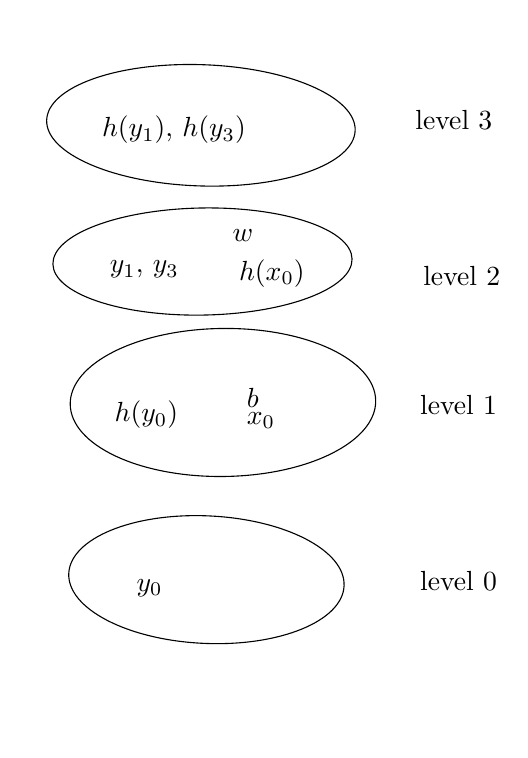
\begin{tikzpicture}[line cap=round,line join=round,>=triangle 45,x=1.0cm,y=1.0cm]
  \clip(0,-2.62) rectangle (6,6.3);
\draw [rotate around={-2.59:(2.27,-0.71)}] (2.27,-0.71) ellipse (1.75cm and 0.81cm);
\draw [rotate around={0.67:(2.48,1.54)}] (2.48,1.54) ellipse (1.94cm and 0.94cm);
\draw [rotate around={0.97:(2.22,3.33)}] (2.22,3.33) ellipse (1.9cm and 0.68cm);
\draw [rotate around={-1.91:(2.2,5.06)}] (2.2,5.06) ellipse (1.96cm and 0.77cm);
\draw (4.86,-0.48) node[anchor=north west] {level $0$};
\draw (4.86,1.76) node[anchor=north west] {level $1$};
\draw (4.9,3.4) node[anchor=north west] {level $2$};
\draw (4.8,5.38) node[anchor=north west] {level $3$};
\draw (1.26,-0.58) node[anchor=north west] {$y_0$};
\draw (0.98,1.68) node[anchor=north west] {$h(y_0)$};
\draw (2.66,1.54) node[anchor=north west] {$x_0$};
\draw (2.66,1.85) node[anchor=north west] {$b$};
\draw (2.56,3.48) node[anchor=north west] {$h(x_0)$};
\draw (0.92,3.46) node[anchor=north west] {$y_1$, $y_3$};
\draw (0.82,5.3) node[anchor=north west] {$h(y_1)$, $h(y_3)$};
\draw (2.48,3.86) node[anchor=north west] {$w$};
\end{tikzpicture}


We want to find $x_0$ s.t. $y_0$ is (or is not) a member of it, and
s.t. it is (or is not) a member of $y_2$ and $y_3$. (We don't have to
worry about $y$s of the same level as $x_0$.)  What we do know is that
there is $w$ s.t. $h(y_0)$ is (or is not) a member of it, and s.t. it
is (or is not) a member of $h(y_2)$ and $h(y_3)$. What we want to do
is doctor $h$ so that this $w$ (or at any rate at least one of these
$w$) is $h$ of something.  But of course doctoring $h$ so that $w$ is
in the range of $h$ has the potential to alter $h(y_1)$ and $h(y_3)$.

Well, what is $h(y_1)$?  It is a judiciously chosen superset of
$h``y_1$.  So we need to know how to find $h$ of members of $y_1$.
Members of $y_1$ are things of level $1$, and $h$ of a thing $a$ of
level $1$ is a judiciously chosen superset of $h``a$.  But $h$ on
level $0$ is just $iota$. so $h(a)$ is a judiciously chosen superset
of $\iota``a$.  Now we want $w$ to be $h$ of some object $b$ of level
$1$.  So $w$ has to be a judiciously chosen superset of $\iota`` b$,
namely $(\iota``b) \cup c$, where $c$ contains no singletons.  And
$b$ must be $\iota^{-1}``(w \cap \iota``V)$ (which i suppose is just
$\iota^{-1}``w$).

So alter that part of $h$ that sends level $1$ into level $2$
(which i suppose we could call $h_{1\inj 2}$) by deciding that $h(b)$
is no longer the old $h(b)$ but is now $w$.  This changes only one
ordered pair in $h_{1\inj 2}$) but of course propagates to $h_{2\inj 3}$,
and changes infinitely many pairs there, and of course that can mean
that the new $h(y_1)$ is not the same as the old $h(y_1)$.  And that
again means that our $w$ may have become useless.  There will be a
new $w$ of course, but there's nothing to say that we won't have
exactly the same problem all over again. The challenge is to have
designed $h$ in such a way that when we tweak it we don't suddenly
find we need a new $w$.  Or better still, seek an $h$ that doesn't
cause us to alter $w$ in the first place.

And how do we do {\sl that}?!

\bigskip

But perhaps, like Wrong Way
Norris\footnote{\url{http://www.montypython.net/scripts/emigration.php}},
our path is in the correct direction but has the wrong sense.  What we should
be doing is trying to prove the following.


\begin{quote}
  Let $\M \models \TZT$.  Let $y_1 \ldots y_n$ be $n$ distinct elements
of $\M$.  Then we can find an injection $h:\M \inj \M$ that preserves
$\in$ and raises types by $1$, s.t. every $y_i$ is a value of $h$.
\end{quote}

This actually sounds quite plausible!


If we can prove it, then we can use it to prove the universal
existential conjecture (or at least that universal-existential
sentences generalise upwards) as follows.

As usual it suffices to consider formul{\ae} of the kind
$(\forall \vec y)(\psi(\vec y) \to (\exists \vec x)(\phi(\vec y, \vec x)))$ 
where $\psi$ and $\phi$ are quantifier-free and $\psi$ is a conjunction of
atomics and negatomics.  We want to show that, whenever $\M$ is a model of \TZT,
$\M\models(\forall\vec y)(\psi(\vec y)\to(\exists\vec x)(\phi(\vec y,\vec x)))$


So fix $\M \models \TZT$ and fix a tuple $y_1 \ldots y_n$ of things in $\M$
instantiating $\psi(\vec y)$.  Use the conjecture to obtain a type-raising
$h$ defined on a terminal segment of $\M$ and elements $y'_1 \ldots y'_n$ of
$\M$ s.t. $h(y_i') = y_i$ for all $1 \leq i \leq n$.  Then we assume that
$(\forall \vec y)(\psi(\vec y) \to (\exists \vec x)(\phi(\vec y, \vec x)))$
holds one level down to obtain witnesses for the $x$istential variables.
We then whack those witnesses with $h$ to obtain witnesses for the
instance of the unshifted version of
$(\forall \vec y)(\psi(\vec y) \to (\exists \vec x)(\phi(\vec y, \vec x)))$.


Now this seems to be just the idea that Zachiri had in 2013!  So why
should it be any different this time?

Clearly we are going to construct $h$ by recursion on levels. $h^{-1}$
can be defined on $y$ objects of the lowest level with complete freedom,
as far as i can see at the moment.

Thereafter we are trying to inject level $n$ into level $n+1$. If $y$
is of level $n+1$ what is $h^{-1}(y)$ to be?  $y$ is to be thought of
as $h``A \cup B$ where $A$ is $y \cap h``V$ and $B$ is disjoint from
$h``V$.  Then $h^{-1}(y)$ is $h^{-1}``A$.  So, given $y$ we have to
identify $A$ and $B$. $A$ is clearly controlled by what is in $y$.
Things at level $n+1$ that are not $y$ objects we don't care about,
but we do have to define $h$ on all the other things are level $n$,
the things that aren't $h^{-1}$ of $y$ objects at level $n+1$.  I
think these remaining things at level $n$ can be sent to their images
in $h$ (i.e., null inflators). Notice that for this $h$ has to be
setlike.  Does this construction create a setlike $h$?  I think the
answer is `yes' beco's the $h$ we construct can be definable with the
$y$ objects as parameters.

\bigskip


\bigskip


\bigskip


Don't we prove somewhere that an $\in$-loop cannot consist entirely of
finite sets?  (yes: it's lemma 15 of Bowler-Forster). Is there an AE
version of this allegation?

The natural assertion ``Every bottomless set contains $V$'' is 
$\forall^*\exists^*\forall^*$
which is the wrong way round.

\bigskip



\section{The Conjectures}

\begin{conjecture}\label{conj:universalexistential1}
Is it the case that every $\forall^1\exists^*$ sentence consistent
with NF$_2$ has a permutation model.
\end{conjecture}

\begin{conjecture}\label{conj:universalexistential2}
Every $\forall^*\exists^*$ sentence refutable in \nf\ is refutable
already in \nf O.
\end{conjecture}

\begin{conjecture}\label{conj:universalexistential3}
$\nf O$ decides all stratified $\forall^*\exists^*$ sentences.
\end{conjecture}

\begin{conjecture}\label{conj:universalexistential4}
Any term model for \nf\ and any model for \nf\ in which all sets are
symmetric satisfies every $\forall^*\exists^*$ sentence consistent
with \nf O.
\end{conjecture}

\begin{conjecture}\label{conj:universalexistential5}
All unstratified $\forall^*\exists^*$ sentences are either decided by
\nf\ or can be proved consistent by permutations relative to any invariant extension of NF.
\end{conjecture}

\begin{conjecture}\label{henkin}
Let us say a {\sl Henkin sentence} is a branching quantifier sentence where
every prefix is  $\forall^*\exists^*$.  Then \TZT\ has a model satisfying
all consistent Henkin sentences.
\end{conjecture}

We cannot strengthen this last conjecture to ``\TZT\ decides all Henkin
formul{\ae}'' beco's there is a Henkin formula that says there is an
external tsau.  And that is true in some models of TST but not all!


\bigskip



\bigskip


Throughout this discussion we will try to keep to the cute mnemonic
habit---due to Quine---of writing a typical universal-existential
sentence with the initial---{universally quantified}---variables as
$\vec y$ (`$y$' for $y$ouniversal) and the existentially quantified
variables as $\vec x$---for E$x$istential).  That was so we can talk
about $y$ variables and $x$ variables.


In earlier versions, conjecture ~\ref{conj:universalexistential3} used
to be ``$\nf_2$ decides all stratified $\forall^*\exists^*$ sentences.


It is known that the term model for \nf O satifies all consistent
$\forall^*\exists^*$ sentences consistent with \nf O.  Putting this
together with conjecture \ref{conj:universalexistential2} suggests
that \nf\ might have a model satisfying all the $\forall^*\exists^*$
sentences consistent with \nf.  (In fact we conjecture that a term
model for \nf\ would be such a model). At the very least it suggests
that the class of $\forall^*\exists^*$ sentences consistent with \nf\
is closed under conjunction.  This also suggests that if conjecture
\ref{conj:universalexistential2} is correct then whenever $\phi$ is a
consistent $\forall^*\exists^*$ sentence consistent with \nf\ then
$\{\pi: \phi^\pi\}$ belongs to some class $\Gamma$ of sets of
permutations that is closed under intersection.  Is $\Gamma$ nicely
defined in terms of a natural topology on the symmetric group on $V$?
It clearly can't mean ``open'' in the usual topology.




\section{A note on the first two conjectures}

The background to these conjectures is that \nf O proves all
$\exists^*$ sentences consistent with LPC, and one naturally wants to
speculate about what happens with formul{\ae} with more quantifiers.

Notice that ``every superset of a self-membered set is self-membered''
is a $\forall^2\exists^1$ sentence consistent with \nf$_2$ (it's true
in the term model) that is not consistent with \nf O, so we cannot
strengthen `\nf O' to `\nf$_2$' in conjecture
~\ref{conj:universalexistential2}.


Every $\forall^*\exists^*$ sentence has a canonical normal form. If we
take the disjunction of all possible conjunctions of atomic and
negatomic formul{\ae} built up from all the $x$ and $y$ variables by
means of $\in$ and $=$, then any $\forall^*\exists^*$ sentence can be
put in the form $(\forall \vec y)(\exists \vec x)$ followed by a
disjunction of some of those conjunctions.  

Let us assume this done.  Now suppose we had started with a
$\forall^1\exists^*$ sentence, and put it into this normal form.
There is only one $y$ variable, and every value that it takes either
is or is not a member of itself, so we know that if our
$\forall^1\exists^*$ sentence is to be satisfiable at all then at
least one of its disjuncts must be a conjunction containing the atomic
conjunct `$y \in y$' and at least one of its disjuncts must be a
conjunction containing the negatomic conjunct `$y \not\in y$'.  This
is because (since $V$ is a set) `$y$' might be interpreted by
something that is a member of itself, and (since $\emptyset$ is a set)
`$y$' might be interpreted by something that is not a member of
itself.

Anything else is going to be false in all models of any theory in
which we can prove the existence of $V$ and $\Lambda$.  Also, this
seems to be about all we can do in the way of weeding out formul{\ae}
that are not going to be satisfiable.  Notice that this line of talk
relies only on things we can prove in $\nf_2$. Hence conjecture
\ref{conj:universalexistential1}.

Now let us consider $\forall^2\exists^*$ sentences. We now have to
consider not just the two formul{\ae} `$y \in y$ and `$y \not\in y$'
but the 32 conjunctions we get by assigning truth values to `$y_1 \in
y_1$', `$y_1 \in y_2$', `$y_2 \in y_1$', `$y_2 \in y_2$' and `$y_1 = y_2$'.

Now in any set theory in which we can find objects satisfying, for
example, $t_1 \in t_1 \wedge t_1 \not\in t_2 \wedge t_2 \not\in t_1
\wedge t_2 \in t_2$ we can argue that if a $\forall^2\exists^*$ is to
be satisfiable at all then at least one of its disjuncts must be a
conjunction containing $y_1 \in y_1 \wedge y_1 \not\in y_2 \wedge y_2
\not\in y_1 \wedge y_2 \in y_2$, because otherwise it could be
falsified in any model by interpreting each `$y_i$' by $t_i$.  Such a
theory is \nf O. As before, this seems to be the only thing we can do
to weed out formul{\ae} that are not going to be satisfiable, so the
corresponding conjecture for $\forall^2\exists^*$ sentences will be
that every $\forall^2\exists^*$ sentence refutable in \nf\ is
refutable in \nf O.  As it happens, \nf O proves every consistent
$\exists^*$ sentence so we do not need to reach for more complicated
theories when considering $\forall^3\exists^*$ sentences. This is why
conjecture ~\ref{conj:universalexistential2} takes the form that it does.  


We can prove that every $\forall^*\exists^*$ sentence consistent with
\nf O is true in the term model of \nf O. (This is proved in the book
somewhere).  What about \nf$_2$?  There is a complication with
$\nf_2$, namely that the term model doesn't satisfy the $\exists^*$
sentence $(\exists x_1 x_2)(x_1 \in x_1 \not\in x_2 \in x_2 \not\in
x_1)$.  So it isn't true that the term model for $\nf_2$ satisfies
every consistent $\forall^*\exists^*$ sentence.  (I think it proves
that, given two self membered sets, one is a member of the other)

OTOH, we do get this:  

\begin{rem}\mbox{\negthinspace}\\
The term model for $\nf_2$ satisfies every $\forall^*\exists^1$
sentence consistent with $\nf_2$.
\end{rem}
\Proof

Let $(\forall \vec y)(\exists x)\Phi$ be a $\forall^*\exists^1$
 sentence consistent with $\nf_2$.  Then for every vector $\vec t$ of
 terms there is an $x$ such that $\Phi$, so all we have to do is
 establish that such a witness can be found among the terms.

$(\forall \vec y)(\exists x)\Phi$ is satisfiable, so fix a model in
 which it is true. (It doesn't matter which one, as the term model is
 unique, and embeds in all models). Express $\Phi$ in DNF, and fix a
 tuple $\vec t$ of terms.  One of the disjuncts is true.  Truth of
 this disjunct tells us that there is a witness $x$ which has certain
 $t$s as members, is distinct from certain other $t$s (if there is a
 clause requiring it to be equal to one of the $t$s then we are done)
 lacks certain other $t$s, and belongs to a final $t$.  This last
 simplification arises beco's a finite conjunction of things like $x
 \in t$ and $x \not\in t$ is equivalent to a single expression of that
 form, complements and intersections of $t$s being $t$s.  If this
 final $t$ is a low set then the witness is already a term. If it
 isn't, then we are looking inside a cofinite set for a set satisfying
 conditions each of which exclude only a moiety of sets.  So there
 must be a witness. \endproof

Something analogous holds for all basic CO models.  The term model for NF$_2$ is the hereditarily finite-or-cofinite sets, least fixed point version.   This needs to be nailed down.

\medskip


In particular this holds for 
$(\forall x)(x \in x \to (\forall y)(y = x \setminus \{x\} \to y \in x))$

$(\forall x)(x \in x \to (\forall y)((\exists z)(z \in y \bic \neg(z \in x \wedge z \not= x)\vee y \in x))$



\medskip

Now the same argument won't work for $\forall^*\exists^2$ sentences
consistent with $\nf_2$, since that could commit us to finding two
witnesses $x_1$ and $x_2$ satisfying $x_1 \in x_1 \not\in x_2 \in x_2
\not\in x_1$. In these circumstances $x_1$ and $x_2$ both have to be
cofinite, and if $x_2$ and $x_2$ are cofinite, one is a member of the
other: if $V\setminus\{a_1\cdots a_n\}$ and $V\setminus\{b_1\cdots b_n\}$
are members of each other then $V \setminus \{b_1 \cdots b_n\}$ must be
one of the $a_i$ and $V \setminus \{a_1 \cdots a_n\}$ must be one of the
$b_i$, contradicting the fact that the subformula relation on terms is
wellfounded. 

\bigskip

\bigskip


What about extending this to $\forall^*\exists^*$ sentences?

Every $\forall^*\exists^*$ sentence is a conjunction of things of the form

$$(\forall \vec y)(A(\vec y) \to (\exists \vec x)(B(\vec x, \vec y)))$$

where $A$ is a conjunction of $\in$ and $\not\in$ between the $\vec y$ and in $B$ all atomics involve at least one $x$.


The point is that if there is more than one $y$ we can get $A$ to
describe a finite structure that is not a substructure of the term
model for \nf$_2$, which means that any $\forall^*\exists^*$ sentence
built up using that $A$ is trivially true in the term model for
NF$_2$.

But we might be working our way back.  Suppose 
$(\forall \vec y)(A(\vec y) \to (\exists \vec x)(B(\vec x, \vec y)))$ 
is a $\forall^*\exists^*$ sentence refutable in \nf$_2$.  Then $A$ must
describe a substructure of \ldots

\section{A note on Conjecture ~\ref{conj:universalexistential2} and Conjecture ~\ref{conj:universalexistential3}}


%I think i can prove conjecture ~\ref{conj:universalexistential3}.

The {\bf finitely generated} models of \TST O are those whose type 0 has only finitely many atoms.

A {\bf partition} $\mathbb{P}$ of a set $X$ is a subset of $\pow X)$ such that $\bigcup
\mathbb{P}= X$ and the members of $\mathbb{P}$ are pairwise disjoint.

If $\mathbb{P}_1$ and
$\mathbb{P}_2$ are two partitions of the same set we say $\mathbb{P}_1$ {\bf refines}
$\mathbb{P}_2$ if every piece of $\mathbb{P}_1$ is a subset of a piece of $\mathbb{P}_2$.

A subset $X' \subseteq X$ {\bf crosses} another subset $p \subseteq X$
if $X' \cap p$ and $X' \setminus p$ are both nonempty.  (That is to
say, $X'$ is not in the field of sets generated by $\mathbb{P}$ if $X'$
crosses a piece of $\mathbb{P}$).

We first prove that every countable model of \TST O is a direct limit of
all the finitely generated models of \TST O.  (The ``all" is important.)

We do this by induction on the number of types.  For reasons which will
become clear we will regard the finitely generated models as starting with
a base type $T_1$ with ${2^n}$ elements and a boolean algebra structure
rather than starting with a base type $T_0$ with $n$ elements and no
structure.  In effect we forget about the bottom type. So the thing we are
going to prove by induction on $k$ is that every countable model of $\TST
O_k$ is a direct limit of {\bf all} finitely generated models of $\TST O_k$.

For the base case we prove that every countable atomic boolean algebra $\B$
there is a family $\B_i: i \in \Nn$ of subalgebras of $\B$ where $\B_i$ has
$i$ atoms, where the inclusion map is a boolean homomorphism and the union
$\bigcup_{i \in \smallNn}\B_i$ is $\B$.

We obtain $\B_{i+1}$ from $\B_i$ by splitting one of the $i$ atoms into
two, effectively adding two new atoms.  To decide which atom to split, and
how to split it, depends on how we wellorder $\B$. We have a fixed
wellordering of $\B$ to order type $\omega$.  At stage 0 we consider $\B_0$
which of course is just the two element boolean algebra containing the top
element and the bottom element.  We make $x_1$ an atom and set $\B_1$ to be
the four element boolean algebra with $x_1$ and $V\setminus x_1$ as atoms.


Thereafter at any stage we have two things in hand:

(i) a most-recently-constructed algebra $\B_i$ and

(ii) an $x_k$ which is to be an element of an algebra soon to be
constructed. (Notice that $i$ and $k$ are not assumed to be the same!
In general $i$ is likely to be much bigger than $k$.)

The set of atoms of $\B_i$ that we have is simply a partition of the atoms
of $\B$ into $i$ pieces. At stage $k$ we consider $x_k$.  $x_k$ will be a
superset of some atoms and disjoint from others. These we do nothing to.
The remaining atoms it crosses.  The atoms are ordered by the
canonical worder of $\B$.  Suppose for example $x_k$ crosses five of the $i$
atoms of $\B_i$, to wit: $c$, $d$, $e$, $f$, $g$ in order.  Then we obtain succesively
$\B_{i+1}$ by splitting $c$ into $c \cap x_k$ and $c \setminus x_k$; then 
$\B_{i+2}$ by splitting $d$ into $d \cap x_k$ and $d \setminus x_k$; then
$\B_{i+3}$ by splitting $e$ into $e \cap x_k$ and $e \setminus x_k$; then
$\B_{i+4}$ by splitting $f$ into $f \cap x_k$ and $f \setminus x_k$; and finally
$\B_{i+5}$ by splitting $g$ into $g \cap x_k$ and $g \setminus x_k$.

What has this achieved?  We now have constructed our sequence of
subalgebras as far as $\B_{i+5}$ and we have ensured that $x_k$ is in the
direct limit.  By iterating this we will eventually ensure that every
element of $\B$ appears, so the direct limit of the sequence of subalgebras
generated in this way is $\B$.

The induction step is similar but messier.

   Let $\B$ be a countable atomic boolean algebra which is the union of
$\tuple{\B_n : n < \omega }$: a $\subseteq$-nested sequence of finite
subalgebras of $\B$. Let $\B^+$ be a countable atomic subalgebra of $\pow
\B)$ containing all singletons. Then there is a sequence $\tuple{\mathbb{P}_i : i <
\omega}$ of finite partitions of $\B$ such that $\mathbb{P}_0$ is the trivial partition with only one piece
and for each $i \geq 1$,

\medskip

$\mathbb{P}_i$ refines $\mathbb{P}_{i-1}$.
$\mathbb{P}_i \subseteq {\B^+}$

$\B_i$ is a selection set for $\mathbb{P}_i$.

\medskip

Further, if we let $\B^+_i$ be the subalgebra of $\B^+$ whose atoms are the
pieces of $\mathbb{P}_i$ (so that $\pow \B_i) \simeq \B^+_i$) then the union of the
$\B^+_i$ is ${\B^+}$.  As before we have a well-ordering $\tuple{x_n : n <
\omega }$ of ${\B^+}$.

We construct the sequence of partitions by recursion. As noted above, $\mathbb{P}_0$
is the trivial partition with only one piece.  Thereafter we procede as follows.

Suppose we have constructed partitions up to $\mathbb{P}_{i-1}$, and we have $x_j$
in hand, where $x_j$ is the first element of $\B^+$ (in the sense of the
canonical ordering) not already a finite union of pieces of $\mathbb{P}_{i-1}$.
We seek a refinement $\mathbb{P}_i$ of $\mathbb{P}_{i-1}$ such that each piece of $\mathbb{P}_i$
contains precisely one element of $\B_i$ and such that $x_j$ is a union of
pieces of $\mathbb{P}_i$.

   How are we to subdivide the pieces of $\mathbb{P}_{i-1}$ to get pieces of
$\mathbb{P}_i$?  Clearly whenever $x_j$ extends, or is disjoint from, a piece of 
$\mathbb{P}_{i-1}$ then we do not need to subdivide that piece in order to get 
pieces for $\mathbb{P}_i$ such that $x_j$ is a union of some of them.  However, 
if $x_j$ crosses a piece $p$ of $\mathbb{P}_{i-1}$ we need to take steps. There 
are other things that may cause us to subdivide $p$ and that is the need 
to ensure that every member of $\mathbb{P}_i$ contains precisely one element of 
$\B_i$.  If $p$ meets $x_j$ and $p \cap x_j$ contains elements from
$\B_i \setminus \B_{i-1}$ then we can partition $p$ into pieces each of which
contains precisely one element of $\B_i \setminus \B_{i-1}$.  Naturally if we can
do this for every piece that meets $x_j$ or its complement success is assured.

However there remains the possibility that $p$ crosses $x_j$ but that $p
\cap x_j$ contains {\sl no} elements from $\B_i \setminus \B_{i-1}$.  This
is grave, because then there is no means of partitioning $p$ into pieces
each of which contains precisely one element of $\B_i$ and whose union is
$p \cap x_j$ (and this of course excludes the possibility of refining
$\mathbb{P}_{i-1}$ into a partition every piece of which contains precisely one
element of $\B_i$ and such that $x_j$ is a union of
pieces).

This means that in these circumstances we have to lower our ambitions.  It
has turned out to be too much to expect $x_j$ to be a union of pieces of
$\mathbb{P}_i$ but we can expect to be able to make it a union of pieces of
$\mathbb{P}_{i+k}$ for some finite $k$.  That will be sufficient, because that way
every $x_j$ will get used up eventually, but can it be done?  We have to go
on throwing in elements of $\B_i$, $\B_{i+1}$, $\B_{i+2}$\ldots $\B_{i+k}$,
until $p \cap x_j$ and $p \setminus x_j$ both meet $\B_{i+k}$.  But
this must happen sooner or later because $\B$ is a union of all the $\B_i$
so any subset of $\B$ (such as $p \cap x_j$) must meet cofinitely many of
them.

   So, to sum up, the step from $\mathbb{P}_{i-1}$ to $\mathbb{P}_i$ is made with an
$x_j$ in mind.  If we can refine $\mathbb{P}_{i-1}$ in such a way that every piece
of the new partition contains precisely one element of $\B_i$ and $x_j$ is
a union of the new pieces, well and good.  Set $\mathbb{P}_i$ to be the new
partition and worry next about $x_{j+1}$.  If we cannot do this, we can at
least refine $\mathbb{P}_{i-1}$ in such a way that every piece of the new
partition contains precisely one element of $\B_i$, and we call that
$\mathbb{P}_i$.  We then attempt the same, starting this time with $\mathbb{P}_i$ and
continuing to worry about $x_j$.

\endproof


Every countable model of \TST\ is a direct limit of {\bf all} finitely
generated models of \TST.

Let $\M$, a countable model of simple type theory, have as its domain a
family $\tuple{\B_n : n < \omega }$ of countable atomic boolean algebras,
where $\B_{n+1}$ is a countable atomic subalgebra of $\pow\B_n)$.  Let
$\B_1$ be a union of an $\omega$-sequence $\tuple{\B_1^i : i < \omega }$.
We then invoke the induction step above repeatedly to obtain, for each $n$,
families $\tuple{\B_n^i : i < \omega }$ of subalgebras and $\tuple{\mathbb{P}_n^i
: i < \omega }$ of partitions as above. Now for each $i < \omega$ consider
the structures $\tuple{\tuple{\B_n^i : n < \omega }, \in }$.  We have
constructed the $\B_n^i$ so that $\B_n^{i+1}$ is an atomic boolean algebra
whose atoms are elements of a partition for which $\B_n^i$ is a selection
set. Thus, if we want to turn the $\tuple{\B_n^i : n < \omega }$ into a
model of simple type theory the obvious membership relation to take is
$\in$ itself. They are models of simple type theory without the axiom of
infinity, and by construction their direct limit is pointwise the $n$th
type of $M$, so the direct limit is $M$ as desired.  \blob\footnote{This
suggests that the obvious product topology on the space of countable models
of \TST\ might be useful \ldots}

There is an obvious modification for \TZT.  Every countable model of \TST\
is a direct limit of all finitely generated models of \TST\ and so is
certainly a direct limit of $\M_1$, $\M_2$ \ldots $\M_n$ where $\M_1$ is
the canonical model where $T_0$ has one element and $\M_{n+1}$ is the
result of deleting the bottom type off $\M_n$ and relabelling.  Now let
$\N$ be an arbitrary countable model of \TZT, and consider a terminal
segment of it.  We have just shown that this terminal segment is a direct
limit of the $\M_n$.  It is a simple exercise to extend this network of
embeddings downwards \ldots

This tells us that every countable model of \TZT\ is a direct limit of
an $\omega^*$ sequence of copies of $\M_1$.

The missing link is a proof of the assertion that there is no
universal-existential sentence (in the language of boolean algebra or
perhaps set theory) which has infinite models but no finite models.

The intention is that once we have this we wrap up the proof as follows.

Let $\phi$ be a existential-universal sentence with an infinite model.
Therefore it has a countable model. Then $\neg \phi$ cannot be true in
arbitrarily large finitely generated models because otherwise $\neg \phi$
would be true in all countable models.  So $\phi$ is true in all suff large
finitely generated models, say all models with at least $n$ atoms.


 If $\neg \phi$ has an infinite model so does the expression ``$\neg \phi
\wedge$ there are at least $n$ atoms". (Indeed they have the same infinite
models!)  But this expression has no finite models.  But unless $\phi$ is
true in all countable models, ``$\neg \phi \wedge$ there are at least $n$
atoms" is an example of a universal-existential sentence with an infinite
model but no finite models.

So if there is no universal-existential sentence (in which language?) which
has infinite models but no finite models then \TST\ decides all
universal-existential sentences.

\subsection{Some other observations that might turn out to be helpful}


First prove that if $(\forall \vec y \in V_\omega)(\exists \vec
x)\Phi(\vec x ,\vec y)$ is a universal-existential sentence consistent
with \TST\ then its type-free version is true in some transitive
wellfounded model of \kf.  Next prove that if $(\forall \vec y \in
V_\omega)(\exists \vec x)\Phi(\vec x, \vec y)$ is a
universal-existential sentence true in some transitive wellfounded
model of \kf then it is true in $V_\omega$.  (This ought to be true
beco's every transitive wellfounded model of \kf\ is an end-extension
of $V_\omega$---also rud functions increase rank by only a finite
amount may 1998).  Then we argue that if $(\forall \vec y \in
V_\omega)(\exists \vec x)\Phi(\vec x ,\vec y)$ is a stratified
universal-existential sentence true in $V_\omega$ then its typed
version has a finitely generated model.

Do we mean true at one type or true at all types?

  Suppose $(\forall \vec y \in V_\omega)(\exists \vec x)\Phi(\vec x, \vec
y)$.  Assume that $\Phi$ is stratified and is in disjunctive normal form.

Since $\Phi$ is stratified there is a stratification of its variables.
This suggests an obvious conjecture.  If `$u$' is of type $n$ why not
restrict the quantifier binding `$u$' to $V_n$ and hope the result to be
true?  How might this go wrong?  One obvious way is exemplified by the
following formula: $$(\forall y)(\exists x_1 \ldots x_{10^{10}})(\bigwedge_{1 \leq i < j \leq 10^{10}} (x_i \not= x_j \wedge (y \in x_i \wedge y \in x_j)))$$

This is only going to be true at sufficiently high types.  What we have to
establish is that this is the {\sl only} way things can go wrong.

First, by reasoning in ZF or Zermelo plus foundation, we argue that every
universal-existential sentence true in $V$ is true in $V_\omega$.

Pause briefly to think about the graph of $\Phi$, by which i mean the
digraph whose vertices are variables with a directed edge from `$y$' to
`$x$' if `$y \in x$' occurs somewhere.  If this digraph has no loops
involving `$x$' variables we procede as follows, making use of the obvious
rank function on `$x$' variables which is available in these circumstances.

Instantiate all the `$y$' variables to names of individual hereditarily
finite sets.  We can import the existential quantifiers past the
disjunctions so that each disjunct is now a string of existential
quantifiers outside a conjunction of atomics and negatomics.  At least one
of these disjunctions is true: grab it. We now want to find witnesses
for---{\sl instantiate}---the `$x$' variables bound by the existential
quantifiers leading that disjunct, and we want to find these inside
$V_\omega$.  (Notice that at this stage we can assume there are no positive
occurrences of `=' within this disjunct, because `$(\exists u)(\exists
v)(\ldots u = v \ldots)$ can be rewritten to remove one of the two
variables.) Some of these variables ``point to" `$y$' variables in the sense
that there is a directed edge from them to one or more `$y$' variables.
Such `$x$' variables must be instantiated by hereditarily finite sets if
they can be instantiated at all, and we know they can be so instantiated
because we are assuming that $(\forall \vec y \in V_\omega)(\exists \vec
x)\Phi(\vec x, \vec y)$. So instantiate them all simultaneously with a tuple
of witnesses in virtue of which we knew that particular instance of
$(\forall \vec y \in V_\omega)(\exists \vec x)\Phi(\vec x, \vec y)$.

Now to instantiate the remaining `$x$' variables. A witness for this sort
of variable must have certain given things as members and certain other
things not as members, so why not simply take it to be the set of things
that it has to have as its members?  Because we might end up thereby
instantiating both `$x_1$' and `$x_2$' to $\{a_1,a_2,\{\emptyset\}\}$, say,
while elsewhere in the formula we are trying to make $x_1 \not= x_2$ true,
so sometimes we have to add silly elements to things to make them
different.  

We then continue by recursion on the rank of `$x$' variables.

This tells us that any true stratified universal-existential expression in
the language of set theory is true in $V_\omega$.

In this connection it may be worth noting that every model of \tst O
${\cal P}$-extends every finitely generated model, so any $\SiP_1$
sentence true in even one finitely generated model is true in all
infinitely generated models.

It is almost certainly time to use the theorem of Ramsey that says
that there is a decision procedure to establish whether or not an
arbitrary $\Pi_1$ sentence has an infinite model. Ramsey claims a
generalisation to $\Sigma_2$ formul{\ae}.

The following remark should be properly spruced up and included in
{\tt TZTstuff.tex}.


\subsection{An old theorem, revived}

We need to distinguish between the L\'evy hierarchy and the $\cal P$
hierarchy.  The L\'evy hierarchy is the usual one used in the ZF
world, where restricted quantifiers don't count, and the $\cal P$
hierarchy is where restricted quantifiers $\forall x \subseteq y$ and
$\exists x \subseteq y$ are allowed.

I have dusted off old notes on ambiguity of $\Sigma^{L\acute{e}vy}_1$
sentences.  I think $\TZT\vdash Amb(\Sigma^{L\acute{e}vy}_1)$. In fact
i suspect that the proof i am about to give might prove something
slightly stronger, namely that \TZT\ proves every consistent
$\Sigma^{L\acute{e}vy}_1$ sentence in the language of \TZT.
\smallpara{I am not quite sure what one means by {\sl consistent} in
  this context but an examination of the construction will reveal it.
  Notice that we cannot work the same trick in NF, beco's the
  existence of a Quine atom is $\Sigma^{L\acute{e}vy}_1$ and is
  certainly not a theorem of NF.}


\begin{rem}\label{64}  $\TZT \vdash Amb(\Sigma^{L\acute{e}vy}_1)$
\end{rem}
                                     
\Proof

We start by observing that $\Sigma^{L\acute{e}vy}_1$ formul{\ae}
generalise upward through end-extensions.  This helps with the
ambiguity question beco's $\M^*$ can be thought of as an end-extension
of $\M$.  Any injection from the bottom level of $\M$ to level 1 of
$\M$ lifts to injections from level $n$ to level $n+1$ for all larger
$n$.  These injections embody an injection from $\M$ into $\M^*$.
Since every subset of a value of this injection is itself a value of
this injection it preserves $\Delta^{L\acute{e}vy}_1$ formul{\ae} and
therefore $\Sigma^{L\acute{e}vy}_1$ formul{\ae} upward.

The hard part is to show that $\Sigma^{L\acute{e}vy}_1$ formul{\ae}
generalise {\sl downwards} as well, in the sense that
$\TZT \vdash \phi^* \to \phi$ for $\phi$ a $\Sigma^{L\acute{e}vy}_1$ formula.

This hard part falls into two cases, depending on whether or not the axiom of infinity holds.


$\bullet$\, We claim that all models of $\TZT + \neg$AxInf satisfy Amb($\Sigma^{L\acute{e}vy}_1$).

Since $\Sigma^{L\acute{e}vy}_1$ sentences generalise upwards then, for any
$\Sigma^{L\acute{e}vy}_1$ sentence $\Phi$, either it is false in all finitely
generated models or there is an $n$ such that it is true in all models
bigger than $n$.  This $n$ is standard if the G\"odel number of $\Phi$ is
standard\footnote{Actually, looking at this again while trying to sell
it to Randall\ldots Is it really true?  It is reminding me of the glitch
in my erroneous proof of Tennenbaum: if your metatheory $T$ is fibbing
then it might tell you, of a nonterminating computation whose gnumber
is concrete, that it halts---in a nonstandard number of steps! Now, if
$\M\, \models\, \TZT+\neg$AxInf, then $|M|$ is non-standard finite, so
it is bigger than all the $n$. This shows that {\sl all} models of
$\TZT+\neg$AxInf satisfy the {\sl same} $\Sigma^{L\acute{e}vy}_1$ sentences.}

\smallskip

$\bullet$\, We know that $\Sigma^{L\acute{e}vy}_1$ sentences generalise upward;
we need to show that if we have AxInf then they also generalise downward.

In fact we will claim something stronger.
\begin{lem}
  Suppose $\phi$ is a $\Sigma^{L\acute{e}vy}_1$ formula and we can
  prove in the arithmetic of \TZT\ that $\phi$ is consistent.  Then
  $\TZT \vdash \phi$.\end{lem}

\Proof

Perhaps we want to strengthen the assumption to ``$\TZT\vdash Con(\TZT) \to Con(\TZT+\phi)$.''

Then, by appealing to the Completeness theorem in $\TZT$, we argue
that $\phi$ must have a transitive model.  The model in which we are
conducting this argument will be an end-extension of this model, and
so will also believe $\phi$.  But the arithmetic of \TZT\ is
ambiguous, so this argument can be run at any level.

\medskip

If that doesn't work, we will need a fall-back.  How about this?
Let $\M$ be a model of \TZT. So suppose some $\Sigma^{L\acute{e}vy}_1$ formula
$A$ is true at some level of $\M$.  Then the arithmetic of $\M$ at some
higher level is cognizant of this fact and knows Con$(A)$.  But arithmetic
is ambiguous, as we showed in remark \ref{63}, so Con($(A)$ is true in the
arithmetic much lower down---as far down as we like.  Now---since we have
AxInf---we can prove the completeness theorem (and as low down as we like).
So: in $\M$ (as low down as we like) there is a model of $A$, and an
$\in$-model at that, and a suitable terminal segment of $\M$ will be an
end-extension of it.  Now $\Sigma^{L\acute{e}vy}_1$ sentences are preserved
under end-extensions, so $\M \models A$---as low down as we like.

\endproof


The Devil---as always---is in the detail.  When \TZT\ proves there is
a model of $A$\ldots what is this model?  It's a set with a binary
relation on it?  What we actually want is a substructure of the model
in which we are working, whose membership relation is the membership
relation of the model. Can we be sure of getting that?]

There now follows my earlier discussion from years ago.

The next step is to show that if $Th(\M) \vdash Con(\phi)$ where $\phi$
is $\Sigma^{L\acute{e}vy}_1$ in the language of $\TZT$ then $M$ contains an
$\in$-model of $\phi$.



First we prove in the arithmetic of $Th(\M)$ that $\phi + Ext$ has a model
$\N$ in the integers.  The elements of this model have a type discipline in
a natural way, and only finitely many types are mentioned.  We construct an
$\in$-model $\N'$ essentially by a Mostowski collapse as follows: the elements
of minimal (internal) type are the same as they were in $\N$, namely particular
integers at (external) type $k$, or whatever.  The objects of (internal) type
1 in $\N'$ are to be the appropriate sets of things of (internal) type 0, and
these will of course be of (external) type $k+1$. And so on, for finitely many
types.  Thus 
\begin{center}
$\TZT+$ AxInf $\vdash Con(\phi)\, \to\, \TZT+$ AxInf $\vdash \phi$ for $\phi \in \Sigma^{L\acute{e}vy}_1$
\end{center}
in slang
$\TZT +$ AxInf reflects $\Sigma^{L\acute{e}vy}_1$
sentences.

Next we need a converse. Suppose $\phi \in \Sigma^{L\acute{e}vy}_1$ is
true at some level of $\M$.  Therefore $\phi$ has a model and this
model can in fact be coded by a set of $\M$.  Therefore $Th(\M)$ knows
that $\phi + Ext$ is a consistent theory.  This allegation is
expressible in the arithmetic of $\M$ and so $Th(\M) \vdash Con(\Phi)$.


Note that this construction cannot work for $\SiP_1$!  $\SiP_1$ formul{\ae} would be a good thing to think about next.  What is the status of Amb$(\SiP_1)$?


\section{Conjecture ~\ref{conj:universalexistential5}: finding permutation models}

Given a $\forall^*\exists^*$ sentence $S$, import all the $\exists$'s
and export all the $\forall$'s.  The result is a formula with
$\forall \vec y$ outside a conjunction of implications each of the form
$$Y \to (\exists \vec x)(\phi(\vec x, \vec y))$$ where $\phi$ is a boolean
combination of atomics and negatomics each one containing an $x$
variable, and $Y$ is of the form 
$$(\bigwedge_{\langle i,j\rangle \in J \subseteq I^2} y_i\, R\, y_j),$$ 
where the `$R$' is either `$\in$' or `$\not\in$'.  The disjunction
of all the $Y$s must be valid, since every consistent $\exists^*$
formula of LPC is a theorem of \nf.  We can now export the
conjunctions, and this shows that $S$ is a conjunction of things
of the form
$$(\forall \vec y)((\bigwedge_{\langle i,j\rangle \in J \subseteq I^2} y_i\, R\, y_j) \to(\exists \vec x)(\phi(\vec x, \vec y))$$

Now a conjunction of two formul{\ae} of this form is another formula
of this form.  This means that without loss of generality we need
consider only formul{\ae} of this form.

Can we restrict attention even further to $\forall^*\exists^*$
sentences of this form where the consequent is the existential closure
of a {\bf conjunction} of atomics and negatomics rather than a boolean
combinations? Sadly, no.  Consider $y_1 \in y_1$ and $y_2 \not\in y_2$.
There is something in $y_1 \XOR  y_2$ but is it in $y_1 \setminus y_2$
or in $y_2 \setminus y_1$?  No reason to suppose either.  But perhaps
if we supply more information, about whether or not $y_1 \in y_2$ and
$y_2 \in y_1$ then we might be able to cut down to a single disjunct.

[This problem is nothing to do with these things being unstratified: 
the same happens with $y_1 \in y_2\, \wedge\, y_3 \not\in y_2$.  There is 
either something in $y_1 \setminus y_3$ or something in 
$y_3 \setminus y_1$ but we don't know which.]

That this is not true is shown by the following case.

$$(\forall y_1 y_2)(y_1 \not\in y_1 \wedge y_2 \in y_2 \wedge y_2 \in y_1 \wedge y_1 \in y_2 \to \\ (\exists x)(x \in y_1 \wedge x \not\in y_2) \vee (\exists x)(x \not\in y_1 \wedge x \in y_2))$$

This is provable beco's of extensionality, but neither $$(\forall y_1
y_2)(y_1 \not\in y_1 \wedge y_2 \in y_2 \wedge y_2 \in y_1 \wedge y_1
\in y_2 \to (\exists x)(x \not\in y_1 \wedge x \in y_2))$$ nor
$$(\forall y_1 y_2)(y_1 \not\in y_1 \wedge y_2 \in y_2 \wedge y_2 \in
y_1 \wedge y_1 \in y_2 \to (\exists x)(x \in y_1 \wedge x \not\in
y_2))$$ are provable because we can find $y_1$ and $y_2$ satisfying the
antecedent with $y_1 \subseteq y_2$ and $y_1$ and $y_2$ satisfying the
antecedent with $y_2 \subseteq y_1$.  Try $y_2 := \bbar{V};\ y_1 :=\{\bbar{V}\}$
for the first case and $y_2 := \bbar{V};\ y_1 :=\bbar{V} \cup \{V\}$ for the second.

\medskip

{\bf Anyway} the idea now is that all we have to do to prove the
$\forall^*\exists^*$ conjecture is to show how to get a permutation
model of anything of the form 
$$(\forall \vec
y)(\mbox{\huge{(}}\bigwedge_{\langle i,j\rangle \in J \subseteq I^2} y_i \in y_j) \to
(\exists \vec x)(\phi(\vec x, \vec y)\mbox{\huge{)}}$$ 
as long as it's consistent
with \nf O.  But is it not the case that every $\forall^*\exists^*$
sentence consistent with \nf 0 is true in the term model for \nf 0?

That suggests considering only permutations that leave \nf O
terms alone, since they have witnesses anyway!

We can't just move things that aren't \nf O terms, since being an \nf
O term is not stratified, so we have to move things are not
``sufficiently like'' \nf O terms.  The idea is that anything
sufficiently like an \nf O term will satisfy the $\forall^*\exists^*$
formula we have in mind at any one time, where ``sufficiently alike''
depends on the formula in question.  So we consider only those
permutations that, say, swap with their complements those things that
are not \nf 0 terms of rank at most $k$ for some concrete $k$.


   Illustrate this by thinking about the assertion that there are no
Boffa atoms.  What witness is there?  


There is something very odd about the case 


$(\forall y_1 y_2)(y_1 \not\in y_1 \wedge y_2 \in y_2 \wedge y_2 \in y_1 \wedge y_1 \in y_2 \to
(\exists x)(x \in y_1 \wedge x \not\in y_2) \vee (\exists x)(x \not\in y_1 \wedge x \in y_2))$

The point is that this is true not because of the behaviour of \nf O
terms, but because of extensionality and classical logic.  There is no
reason to suppose that the witnesses will be easy to find.


\section{Positive results obtained by permutations}
%\section{Results positive for conjecture ~\ref{conj:universalexistential5} obtained by permutations}

Let's have a section on $\forall^1\exists^*$ sentences.  The point is
that the difficulty with extensionality (no definable witnesses)
cannot occur if there is only one $y$ouniversally quantified variable.

Is it the case that every $\forall^1\exists^*$ sentence consistent
with NF$_2$ has a permutation model?   This is conjecture 1.

Is the set of $\forall^1\exists^*$ sentence consistent with NF$_2$
closed under conjunction? The set of $\forall^1\exists^*$ sentences is
closed under conjunction

\bigskip


Many of these are published, and collected in Forster [1991].  Here are
some new ones.

\subsection{The size of a self-membered set is not a concrete natural}

Boffa has made some progress on this front.  He has proved that, if
the axiom of counting holds, there is a permutation $\pi$ such that in
$V^\pi$ there is no self-membered finite set.  A little adjustment
strengthens the conclusion and weakens the assumption slightly.

\begin{rem}\label{ref:boffapermutation}
If \nf+\AxC\ is consistent so is \nf+\AxC+ ``Every self-membered set maps onto \Nn''.
\end{rem}

\Proof
Let $X$ be the collection of sets that do not map onto \Nn.  If
$x$ is such a set, then the set of $n \in \Nn$ such that $\{n\} \times
V$ meets $x$ is finite, and will have a last member.  Add 1 to this
last member to get a number we will call $n_x$. $n_x$ has the feature
that $(\forall m \geq n_x)((x \cap (\{m\} \times V)) = \Lambda)$.  $Tn_x$
is the same type as $x$ and so the permutation $$\prod_{x \in
X}(x,\tuple{Tn_x,x})$$ is a set.  Notice that if $x \in X$
then $\tau`x$ is infinite and not equal to $x$.

Now suppose $x \in \tau`x$. To prove that in $V^\tau$ every
self-membered set is infinite it will suffice to show that $\tau `x$
is infinite. We will assume \AxC\ and prove that $\tau `x$ has a
countable partition. 

If $x$ is fixed then $x$ is infinite so $\tau`x$ (which is $x$) is
infinite as desired.  If $x$ is not fixed there are two cases to
consider.

(i) $x \in X$.  Then $\tau`x$ is infinite by construction.

(ii) $\tau`x \in X$.  Then $x = \tuple{Tn_{\tau`x},\tau`x}$. But also
$x \in \tau`x$ so $\tuple{Tn_{\tau`x},\tau`x} \in \tau`x$.  Now
$n_{\tau`x}$ has been chosen to be so large that no ordered pair
$\tuple{m, y}$ is a member of $\tau`x$ for any $ \geq n_{\tau`x}$.  So, to get
a contradiction all we need is $Tn_{\tau`x} \geq n_{\tau`x}$.  The simplest way
to get this is to assume \AxC.

\endproof

(Originally Boffa had taken $n_x$ to be the {\sl first} $n$ s.t.
$\{n\} \times V$ does not meet $x$.  That way he needs the whole of
the axiom of counting.)  Friederike K\"orner and i both noticed that
to make this proof work it is sufficient to have a (set) function $f:
\Nn \to \Nn$ such that $(\forall n)(f(Tn) \geq n)$.  I propose to
call such functions {\bf K\"orner functions}. If we have such a
function we swap $x$ (when $x$ is finite) with $\tuple{f(Tn_x),x}$
instead of $\tuple{(Tn_x),x}$.  Indeed in those circumstances we can
do something even better.

\begin{rem}

If there is a function $f: \Nn \to \Nn$ such that $(\forall n)(f(Tn) \geq
n)$ then (letting $\pi$ be the permutation 

$$\prod_{|x| \in \smallNn}(\tuple{f(Tn_x),x},x)$$

that swaps $x$ with
$\tuple{f(Tn_x),x}$ for $x$ finite) we find that in $V^\pi$ the 
membership relation restricted to finite sets is wellfounded.

\end{rem}

\Proof 

Suppose $V^\pi \models x \in y \wedge |x|\in \Nn \wedge  |y| \in \Nn$.
Then $\pi(x)$ and $\pi(y)$ are both finite and $x \in \pi(y)$.  We will show
$n_{\pi(x)} < n_{\pi(y)}$.  Since $\pi(x)$ is finite, $x$ must be
$\tuple{f(Tn_{\pi(x)}), \pi(x)}$.  But then, since $x \in \pi(y)$, the first
component of $x$ must be less than $n_{\pi(y)}$, so $f(Tn_{\pi(x)}) <
n_{\pi(y)}$.  But we have $n_{\pi(x)} < f(Tn_{\pi(x)})$ by choice of $f$ so
$n_{\pi(x)} < n_{\pi(y)}$ as desired.  \endproof

(In fact we can swap $x$ and $\tuple{x,f(Tn_x)}$ as long as $x$ does
not map onto \Nn. So we can set $\pi := \prod (x,\tuple{x,f(Tn_x)})$
taking $(x,\tuple{x,f(Tn_x)})$ to be the identity if $n_x$ is
undefined.)

Friederike K\"orner then showed that it is consistent relative to \nf\ that
there should be $n \in \Nn$ such that for all greater $m$ we have $m < Tm$,
and that means there is such an $f$, namely $\lambda x.($if $x < n$ then
$n$ else $x)$. Let us call natural numbers $k$ s.t. 
$(\forall n \in \Nn)((n+k) < T(n+k))$ {\bf K\"orner numbers}.

The significance of K\"orner numbers is that if there is a K\"orner
number then there is a K\"orner function, a function $f:\Nn\to \Nn$
such that $(\forall n \in \Nn)(n \leq f`Tn)$.  The existence of such a
function commuting with $T$ is of course equivalent to \AxC, but this
is weaker, and implies that there is a permutation model in which $\in
\restric FIN$ is wellfounded (which indeed was how we found it!).  Given the
desire to find cardinal arithm\'etic equivalents for all modalised sentences
it is natural to try to find a converse \ldots

The following result uses ideas of Boffa-P\'etry from \cite{}
\begin{rem}\mbox{\negthinspace}\\
  
If \nf\ is consistent so is \nf\ + ``No strongly cantorian set is self-membered''.
\end{rem} 
\Proof

For $\alpha \in T``NO$ set 

\begin{itemize}
\item $F(\alpha, x) = \{u \in x: (\exists y)(u = \tuple{V,T^{-1}\alpha,y})\}$

\item $\mu(x) = $ the least $\alpha \in T``NO$ such that $F(\alpha,x) = \emptyset$ if there
      is one, = $V$ otherwise.
\end{itemize}

Note the following:
\begin{enumerate}
\item $stcan(x) \to (\exists \alpha \in T``NO)(F(\alpha,x) = \emptyset))$;
\item If $stcan(x)$ then $\mu(x)$ is a strongly cantorian ordinal;
\item For all $x$, $(\forall y)(\tuple{V,T^{-1}(\mu(x)),y} \not\in x)$.
\end{enumerate}


\marginpar{If we alter the definition of $\mu$ so it picks up the sup
of the nonempty $F$s rather than the first empty $F$ we have to be
sure that (ii) remains true.  It will be true if only strongly
cantorian ordinals can have strongly cantorian cofinality.  But perhaps
that's not even plausible....}


Then set $$\pi = \prod_{x \not\in |V|}(x, \tuple{V, \mu(x),x})$$


I now think that---assuming that this works at all---it establishes
that $\in$ restricted to strongly cantorian sets is wellfounded.  To
that end, suppose $V^\pi$ believes that $x$ is a member of $y$ and
both are strongly cantorian.  We will show that $\mu(\pi(x)) <
\mu(\pi(y))$.

So $\pi(x)$ and $\pi(y)$ are both strongly cantorian and therefore
cannot be nasty ordered triples.  So it is $x$ and $y$ that are the
nasty triples, and we must have $x = \tuple{V,\mu(\pi(x)),\pi(x)})$
and $y = \tuple{V, \mu(\pi(y)),\pi(y)})$

We also have $x \in \pi(y)$, which is to say that the triple $x =
\tuple{V,\mu(\pi(x)),\pi(x)})$ is one of the triples in $\pi(y)$.  

We want $\mu(\pi(x)) < \mu(\pi(y))$.  $\pi(x)$ is strongly cantorian,
so $\mu(\pi(x))$ is a strongly cantorian ordinal.  \marginpar{I think
  we have to modify the definition of $\mu(x)$ to be the sup of
  nonempty $F$s rather than the first nonempty one \ldots}


This will work as long as $cf(\Omega)$ is not strongly cantorian.  In
fact i suspect that it will show that membership restricted to small
sets is wellfounded as long as $cf(\Omega)$ is not small.


\endproof



So let's try to generalise the Boffa-P\'etry construction

\smallskip

For $\alpha \in T``NO$ set 

\begin{itemize}
\item $F(\alpha, x) := \{u \in x: (\exists y)(u = \tuple{V,T^{-1}\alpha,y})\}$

\item $\mu(x) := $sup$\{\alpha + 1 \in T``NO: F(\alpha,x) = \emptyset\}$ 
if this sup is defined, = $V$ otherwise.
\end{itemize}

Note the following:
\begin{enumerate}
\item If $x$ is small then $\mu(x)$ is not $V$;
\item For all $x$, $(\forall y)(\tuple{V,T^{-1}(\mu(x)),y} \not\in x)$.
\end{enumerate}

Then set $$\pi = \prod_{x \not\in |V|}(x, \tuple{V, \mu(x),x})$$

(Perhaps we don't need to swap everything smaller than $V$: it may be
that swapping only small things will do; but we shall see.)


We shall attempt to show that, in $V^\pi$, $\in$ restricted to small
sets is wellfounded.  So let $x$ and $y$ be such that $V^\pi$ believes
$x \in y$ and that both $x$ and $y$ are small.  We will (we hope)
infer from this that $\mu(\pi(x)) < \mu(\pi(y))$.

Assuming that smallness is a property preserved under surjection we
know that $V^\sigma$ believes $x$ to be small iff $\sigma(x)$ was
small in $V$.  So in this context we infer that $\pi(y)$ and $\pi(x)$
are both small and so cannot be nasty ordered triples.  So it is $x$
and $y$ that are the nasty triples, and we must have $x =
\tuple{V,\mu(\pi(x)),\pi(x)})$ and $y = \tuple{V,
  \mu(\pi(y)),\pi(y)})$

We also have $x \in \pi(y)$, which is to say that the triple $x =
\tuple{V,\mu(\pi(x)),\pi(x)})$ is one of the triples in $\pi(y)$.  
from which $\mu(\pi(x)) < \mu(\pi(y))$ is immediate \endproof

So we seem to have shown that: 
\begin{quote} if $cf(\Omega)$ is not small, then
$\poss(\in \restric$ small sets is wellfounded$)$.
\end{quote}  

There doesn't seem to be anything special about the choice of $\Omega$ here

\bigskip


It's worth remembering that in Boffa's original construction $\mu$
picks up the first empty $F$ rather than the sup of the nonempty $F$s.
I thought this was wasteful but actually the difference between his
definition and my modification of it is the same as the difference
between the definition of grundyrank on a wellfounded structure and
the definition of rank, so it might be something natural and meaningful.


\medskip

H I A T U S

\medskip

It seems that we should be able to do better than this. Suppose there
is a function $f: NO \to NO$ such that $(\forall \alpha)(f(T\alpha)
\geq \alpha)$.   Let $\alpha_x$ be the first ordinal that is bigger 
than every ordinal in \fst$``x$. $\alpha_x$ is defined as long as $x$ 
is small in the sense of not being mappable onto a cofinal subset of 
$NO$.  Then let $\pi$ be the permutation that swaps $x$ with 
$\tuple{f`(T \alpha_x),x}$ for $x$ small then in $V^\pi$ the 
membership relation restricted to small sets is wellfounded.

{\bf Can we tweak Andr\'e's proof to show that Con(\nf) $\to$ Con(\nf +
$\in\restric stcan$ is wellfounded)?}

What can we say about the idea that there is an $f: NO \to NO$ s.t.
$f(T\alpha) \geq \alpha$?  Suppose there is such a function, and let
$X$ be a cofinal subset of $T``NO$. Then $f``X$ is a cofinal subset of
$NO$ so $cf(NO) \leq cf(T``NO) = T(cf(NO))$.  For the other direction
sse, to take a straightforward case, that $cf(NO) = \omega$.  To get
such an $f$ (try it!) we would need \AxC.

Boffa has a conjecture that 
\begin{conjecture}
It is consistent with \nf\ that $(\forall x)(x \in x \to |x| = |V|)$
\end{conjecture}

The dual of this is $(\forall x)(x \not\in x \to |V\setminus x| =
|V|)$.  Now if these two hold simultaneously we infer $(\forall
x)(|x| = |V| \vee |V\setminus x| = |V|)$.  This is
stratified and so is certainly not going to be provably consistent by
means of permutations. It is known that there are models of ZF in
which the real line can be split into two smaller pieces.  Richard
Kaye's idea for a counterexample to $(\forall x)(|x| = |V|
\vee |V\setminus x| = |V|)$ is $\{y: |y| < |V|\}$.  In view
of what follows we should also consider $\{y: |y| \not\geq^*
|V|\}$.


If we think of Bernstein's
lemma, all it tells us is that $(\forall x)(|x| = |V| \vee
|V\setminus x| \geq_* |V|)$.  

 If
$|x| \not\geq_* |V|$ we say that $x$ is {\bf small} and if
$|V\setminus x| \not\geq_* |V|$ we say $x$ is {\bf co-small}. By
Bernstein's lemma a set cannot be simultaneously co-small and
small. (Beware: not everything the same size as a co-small set is
co-small: every co-small set is of size $|V|$ but not {\sl vice
versa}. However, nothing the size of a co-small set is small.)

  This suggests that we
might be able to tackle a weaker version by permutations, namely:

\begin{conjecture}\label{conj:boffa1}
\nf$\vdash \poss (\forall x)(x \in x \to |x| \geq_* |V|)$
\end{conjecture} 

We can make a small amount of progress with this version of the
conjecture.  

\verb#\begin{digression}#
\begin{small}
\begin{quote}
\begin{quote}{\bf Some remarks on Quine pairs}\end{quote}
In what follows we will be using ordered pairs in the
style of Quine.  That is to say, we set $\tuple{x,y} = \theta_1``x 
\cup \theta_2``y$, where $\theta_1$ and $\theta_2$ are homogeneous 
bijections between $V$ and two other sets $\theta_1``V$ and
$\theta_2``V$ s.t. $\theta_1``V = -\theta_2``V$. Quine actually
provides two such functions $\theta_1$ and $\theta_2$ but we do not
need to know anything more about them than i have just said. \fst$(x)$
is the first component of the ordered pair $x$.

The advantage Quine pairs are usually supposed to have is that they
ensure the ``$x = \tuple{y,z}$'' is homogeneous.  There are other
advantages as well. If we need a disjoint union function $x \sqcup y$
then $\tuple{x,y}$ would do.  $\tuple{V, \subseteq, - \ldots}$ is a
boolean algebra, and so is $V \times V$.  The Quine pairing function
is actually an {\bf isomorphism} between $V \times V$ and $V$.  Thus,
$V \setminus\tuple{x,y} = \tuple{V\setminus x,V\setminus y}$, 
$\tuple{x\cap y, z} = \tuple{x,z} \cap \tuple{y,z}$, and so on.  
Some of this will be useful in what follows.

Of course this is less attractive in the context of \zf, but similar
results hold.  One should also think about the smallest number of types
with which one can define the two theta functions. Is now the time to go
back and look at Joel Friedman Some set-theoretical partition theorems
suggested by the structure of Spinoza's God. SYNTHESE v 27 (1974) pp
199-210

\end{quote}
\end{small}
\verb#\end{digression}#
\begin{rem}\label{rem:metaboffa}\mbox{\negthinspace}\\
If $$(\forall x)(x \in x \to |x| \geq_* |V|)$$ is consistent
with \nf, so is

$$(\forall x)(x \in x \to |x| \geq_* |V|)\wedge 
 (\forall x)(| V\setminus x| \not\geq_* |V| \to x \in x)$$
\end{rem}

\Proof

The two conjuncts are duals of each other, so one is consistent iff
the other is.  So let us start with a model $V$ satisfying
$$(\forall x)(|V\setminus x| \not\geq_* |V| \to x \in x)$$ We want to
swap every small set $x$ with $\langle V\setminus \fst``x,x \rangle$
but to do this we must check that if $x$ is small then $\langle
V\setminus \fst``x,x \rangle$ isn't (otherwise we would have to swap
that with $\langle V\setminus \fst``\langle V\setminus \fst``x,x
\rangle,\langle V\setminus \fst``x,x \rangle \rangle$ and the
definition would not be consistent.) We will show that if $x$ is small
$\langle V\setminus \fst``x,x \rangle$ is not small, and {\sl vice
  versa}.

Suppose $x$ is small. $\langle V\setminus \fst``x,x \rangle$ is a
superset of $\theta_1``(V\setminus \fst``x)$.  Now $\fst``x$ is a
surjective image of a small set and is therefore small. Therefore
$V\setminus\fst``x$ is a co-small set, and $\theta_1``(V\setminus
\fst``x)$, being the same size as a co-small set, is at least not
small, so its superset $\langle V\setminus \fst``x,x \rangle$ is not
small either.

For the converse suppose $\langle V\setminus \fst``x,x \rangle$ is
small.  If $\langle V\setminus \fst``x,x \rangle$ is small, then so is
its subset $\theta_1``(V\setminus \fst``x)$.  But if
$\theta_1``(V\setminus \fst``x)$ does not map onto $V$ neither does
$V\setminus\fst``x$.  So $\fst``x$, being the complement of a small
set, is co-small.  But if $\fst``x$ is co-small, $x$ cannot be small.

(If we were to try to prove an analogous result with ``small'' meaning
``smaller than V'', this is where the proof would break down. We
cannot show that if $x$ is smaller than $V$ then $\langle V\setminus
\fst``x,x \rangle$ isn't. As far as we know $x$ could be smaller than
$V$ but $\fst``x$ could be the whole of $V$.  Well, that last bit
isn't true but we still have to be careful.)


Now we can safely set

$$\pi = \prod_{|x| \not\geq_* |V|}(x,\langle V\setminus \fst``x,x \rangle)$$



We will verify the two conjuncts separately.

$$V^\pi \models (\forall x)(|x| \not\geq_* |V| \to x \not\in x)$$
This is
$$V \models (\forall x)(|x| \not\geq_* |V| \to \pi`x \not\in x)$$
\marginpar{Surely we mean `$x \not\in \p(x)$'\ldots?}
We procede by a case analysis:
\begin{itemize}
\item If $x = \pi`x$ then $x$ was not small, because all small things are moved. Therefore
      the antecedent is false and the conditional is true.
\item If $x \not = \pi(x)$ and $x$ is small, then $\pi(x) = \langle V \setminus \fst``x,x \rangle$.
      Since $x$ is small, $\fst``x$ (which is a surjective image of $x$) is also small,
      so $V\setminus\fst``x$ is co-small, and therefore---by hypothesis---a member of itself.
      Therefore $\langle V \setminus \fst``x,x \rangle \not\in x$, which is to say $\pi(x) \not\in x$.
\item If $x \not = \pi(x)$ and $x$ is not small, then the antecedent is false and the conditional
      is true.
\end{itemize}

We also want the dual to hold in $V^\pi$, as it did in $V$. So we want
$$V^\pi \models (\forall x)(|V \setminus x| \not\geq_* |V| \to x \in x)$$
This is
$$V \models (\forall x)(|V \setminus \pi(x)| \not\geq_* |V| \to x \in \pi(x))$$
As before, we do a case analysis. \begin{itemize}
\item If $x$ is fixed, the result is true because it was true in the base model by hypothesis.
\item If $x$ is small, then $\pi(x) = \langle V \setminus \fst``x,x
  \rangle$. This is $\theta_1``(V \setminus \fst``x) \cup
  \theta_2``x$, so $V\setminus\pi(x) = \theta_1``(\fst``x) \cup
  \theta_2``(V \setminus x)$. But if $x$ is small, $V\setminus x$ is
  co-small, and so $\theta_2``(V \setminus x)$---being the same size as
  a co-small set---cannot be small. So its superset
  $\theta_1``(\fst``x) \cup \theta_2``(V \setminus x)$ isn't small
  either.  But $\theta_1``(\fst``x) \cup \theta_2``(V \setminus x)$ is
  $V\setminus\pi(x)$. Therefore $V\setminus\pi(x)$ is not small so the
  antecedent is false, and the conditional true.
\item If $x$ is not small, it is $\pi(y)$ for some small set $y$.  So 
$\pi(x)$ is small, and so $V\setminus\pi(x)$ is co-small and the 
antecedent is false.
\end{itemize}

\endproof

Another observation in the same style is the following:

\begin{rem}\label{rem:small}\mbox{\negthinspace}\\
If there is a wellfounded set $X$ s.t. $\powk{\kappa} X) \subseteq X$
then there is a permutation model in which $\in$ restricted to sets
without partitions of size $\kappa$ is wellfounded.
\end{rem}
\Proof ($\kappa$ actually has to satisfy the extra condition: $\alpha
\leq^* \kappa \to \alpha \leq \kappa$, but $\kappa$ will be an aleph
in all current applications---for the moment at least.)  Let $\pi$ be 
the product 
$$\prod_{|x| \not\leq^* \kappa}(x, \tuple{V \setminus x, (\snd``x \cap X)})$$ 
of the transpositions $(x, \tuple{V \setminus x, (\snd``x \cap X)})$ 
over all $x$ without partitions of size $\kappa$.

Let such sets be ``$\kappa$-small'', at least for the duration of this
proof.  This is basically a Boffa permutation (as in remark
\ref{ref:boffapermutation}).  However, there is a slight wrinkle.
With Boffa's original permutation much use was silently made of the
fact that the second components of the ordered pairs in the story were
{\sl large}, being natural numbers.  This ensured that whenever $\pi$
moved $x$, then $\pi(x)$ was large iff $x$ was small.  This was essential 
to the plot, and remains essential here.  Now $\snd``x \cap X$ is small 
if $x$ is, so in order to achieve ``whenever $\pi$ moves $x$, then 
$\pi(x)$ is large iff $x$ is small'' we need to do something to the 
$\fst$ element of the pair it make {\sl it} large instead. This is what 
complementation is doing.

Let's just check this.  If $x$ is $\kappa$-small then $\pi(x)$ is an
ordered pair one of whose components is $V\setminus x$ wot ain't nohow 
$\kappa$-small, so $\pi(x)$ is not $\kappa$-small.  Now suppose 
$\pi(x) \not= x$ and $\pi(x)$ is not small.  Then it is 
$\tuple{V \setminus x, \snd``x \cap X}$.  By design of $\pi$, this 
object can only have been moved from $x$, so $x$ was $\kappa$-small.

Suppose $V^\pi$ thinks that that $x \in y$ and both are
$\kappa$-small.  This last tells us---as we have seen---that $y$ must
be $\tuple{V \setminus \pi(y), (\snd``\pi(y) \cap X)}$, and $x$ must be
$\tuple{V \setminus \pi(x),(\snd``\pi(x) \cap X)}$.  Now $x \in \pi(y)$ so
$\snd(x) \in \snd``\pi(y)$.  Now $\snd(x) = \snd``\pi(x)\cap X$ so
$\snd(x)$ is at least a subset of $X$, and it's $\kappa$-small because
it's a subset of $\snd``\pi(x)$ which is a surjective image of
$\pi(x)$ which is $\kappa$-small.  So it's a $\kappa$-small subset of
$X$ and is therefore a member of $X$, since $\powk{\kappa} X)
\subseteq X$.  So $\snd(x)$ is a member of both $\snd``\pi(y)$ and
$X$, so it's a member of $\snd``\pi(y) \cap X$, which is $\snd(y)$ so
$\snd(x)\in \snd(y)$.

Thus we have shown that: whenever $V^\pi$ thinks that $x \in y$ and both 
$x$ and $y$ are $\kappa$-small, then $\snd(x) \in \snd(y)$, and we also 
know that both of these things are in $X$.  In other words, if we let $K$
be the set of things that $V^\pi$ believes to be $\kappa$-small, then
$\snd$ is a homomorphism from $\tuple{K, \in_\pi}$ to $\tuple{X,\in}$.
$X$ is wellfounded by assumption, so $\tuple{K, \in_\pi}$ must be too.

\endproof

It might be worth considering an indexed family of permutation models
generated as follows.  Given an $X$ as above (minus the wellfoundedness
condition) let $\pi_X$ be the permutation defined as above.  Order them
according to the partial order on the $X$'s.  The result is a Kripke model
of something-or-other.

It would be very nice to have a converse to remark ~\ref{rem:small}.

My version of Boffa's conjecture is: co-small implies self-membered.
(A special case of) the universal-existential conjecture is:
self-membered implies meets everything in the sublattice generated by
the values of $B$.  The conjunction of these two implies that every
co-small set meets everything in the sublattice generated by the
values of $B$.  This we know to be true.

\subsubsection{Can we spice this up to lattices generated by free bases for $V$?}

%Dick and Valeria's leaving party nov 1998

How many bases are there? How big are they?  How big are their elements?

Given any basis i can swap any element with its complement, so the
number of bases is at least two-to-the size of any basis.

The $\forall^*\exists^*$ conjecture implies that if $x\in x$ then $x$
meets every element of the standard basis.  How about every element
of every basis?  Doesn't that sound a bit like ``Every self-membered
set generates $\tuple{V, \subseteq, -}$''?

I claim the following\begin{enumerate}
\item ``Every self-membered set generates $\tuple{V, \subseteq, -}$'' 
is $\forall^*\exists^*$;
\item If $\alpha$ is the size of a generating set then $T|V| \leq 2^\alpha$;
\item If $2^\alpha = T|V|$ then there is a basis of size $\alpha$.
\end{enumerate}

The first is easy to check.  It is $(\forall y \in y)(\forall y_1
y_2)(\exists x \in y)(y_1 \in x \bic y_2 \not\in x \vee y_1 =
y_2)$. The following generalisation of item (i) merits attention: $x
\in x \to x \cap \pow x)$ generates $\pow x)$.  It's not
$\forall^*\exists^*$ but it's natural.

(ii) Follows beco's every singleton is an intersection of basis 
elements and complements of basis elements.

(iii) Sse $F:\iota``V \bic \pow X)$ is a bijection.  Each singleton
$\{y\}$ corresponds to a subset $X'$ of $X$, and we deem that $\{y\}$
is the intersection of the basis elements belonging to $X'$ and the
complements of the basis elements in $X \setminus X'$.  So $f`x$ must
be $\bigcup\{y \in \iota``V: x \in F(y)\}$. Then $f``X$ is a basis.


small$(x) \to x \not\in x$; Hsmall$(x) \to WF(x)$; $\in\restric$small is
wellfounded.
\subsection{Bases for the irregular sets}

Something about this in coret.tex

A set is {\bf irregular} iff it meets all its members. A basis for the
irregular sets is a set that meets every irregular set.  Some of the
theorems we have proved can be expressed as facts about bases.
Membership restricted to finite sets being wellfounded is the same as
the infinite sets forming a basis.  Can the uncountable sets form a
basis?  We shall see!  However the set of co-small sets isn't big
enuff to be a basis.  If $X$ is irregular so is $B``X$, and no member
of $B``X$ is co-small!

Still, there is a large gap between the set of uncountable sets and 
the set of co-small sets.


\subsection{Membership restricted to ideals and their filters}
\label{history} 

Need to fit Button-Hurkens into here somewhere, and take this section
by the scruff of the neck.

Button-Hurkens:  If $X$ is a bottomless (aka irregular) set of ideals, then $\bigcap X$ contains all wellfounded sets.

\bigskip


History seems to lead us thus.  We start off with a notion of
smallness (like {\sl finite}) and notice that no small set seems to be
a member of itself.  We then conjecture that $\in$ restricted to small
sets is wellfounded, and finally that $R$ (defined by $R(x,y)$ iff $x$
and $y$ are both small or co-small and $x \in y \bic y$ is small) is 
wellfounded. But it's no good if the ideal of small sets is prime:

\begin{rem}\mbox{\negthinspace}\\
\mbox{Let $I$ be a prime ideal and consider the relation $x\, R\, y$ defined as 
$x \in y \bic y \in I$.}

Then $R$ is not wellfounded.
\end{rem}

\Proof

In those circumstances $\in \restric I$ is wellfounded and 
$\not\in \restric I$ is wellfounded.  Find somehow sets $a$ and $b$ 
such that $a \not\in a \cup b$ and $b \in a \cap b$. (This is easy 
to arrange: set $a := \bbar{\Lambda}$; $b:= B(V)$.)  Then $a \not\in a$ 
so $a \in I$ and $b\, R\, a$ `cos $b \in a$.  $b\in b$ so $b \not\in I$ 
and $a\, R\, b$ `cos $a \not\in b$.  Then $R$ is not wellfounded. \endproof

(Notice that this refutation uses the \nf O axiom, so we might get away
with the following relation over Church-Oswald models of $\nf_2$ might
be wellfounded (at least when the $k$oding function is nice):
$x \inn y \bic (\snd(k^{(-1)}(y)) = 0)$.)

There are two steps involved:  
\begin{quote}
(i) Move from ``$\in$ restricted to $I$ has no loops of diameter 1,
2 \ldots'' to ``$\in$ restricted to $I$ is wellfounded'' 

(ii) to  Move from ``$\in$ restricted to $I$
is wellfounded'' to ``$R$ is wellfounded''.
\end{quote}
How difficult are these?  Where $I = FIN$, (i) seems clear enuff. How
about (ii)? Perhaps the permutation making $\in \restric FIN$ wellfounded 
(or some variant of it) will also make this other relation wellfounded.

Try the following permutation: if $x$ is finite, swap $x$ with
$\tuple{f(Tn_x), x}$; if $x$ is cofinite swap $x$ with
$\tuple{f(Tn_{V\setminus x}), V \setminus x}$.  (I think we will need a sort-of 
rank function that sends $x$ to $n_{V \setminus x}$ if $x$ is finite and 
to $n_{V \setminus x}$ if $n$ is cofinite. Call this $n'_x$)


We want $V^\pi \models $``$R$ is wellfounded''.  Now
$V^\pi \models\, \, x\, R\, y$ iff

$\pi(x)$ and $\pi(y)$ are both finite-or-cofinite and $x \in \pi(y) \bic
\pi(y)$ is finite. 

Want to show that if $V^\pi \models\, \, x\ R\ y$ then $n'_{\pi(x)} < n'_{\pi(y)}$.

case 1: $\pi(y)$ is finite.  Then $y = \tuple{f(Tn_{\pi(y)}), \pi(y)}$. 

\begin{enumerate}\item{Case 1a}
$\pi(x)$ is finite. Then $x$ must be $\tuple{f(Tn_{\pi(x)}), \pi(x)}$.
But then, since $x \in \pi(y)$, the first component of $x$ must be less
than $n_{\pi(y)}$, so $f(Tn_{\pi(x)}) < n_{\pi(y)}$.  But we have
$n_{\pi(x)} < f(Tn_{\pi(x)})$ by choice of $f$ so $n_{\pi(x)} <
n_{\pi(y)}$ as desired.


\item{case 1b}  $\pi(x)$ is cofinite. Then $x$ must be
$\tuple{f(Tn_{V \setminus \pi(x)}), V \setminus \pi(x)}$. But then, since 
$x \in \pi(y)$, the first component of $x$ must be less than $n_{\pi(y)}$, 
which is to say $f(Tn_{V \setminus \pi(x)}) < n_{\pi(y)}$ and therefore (by 
choice of $f$) $n_{V \setminus \pi(x)} < n_{\pi(y)}$.
\end{enumerate}

case 2 $\pi(y)$ is cofinite.  Then $y = \tuple{f(Tn_{V \setminus \pi(y)}), V \setminus \pi(y)}$.

Case 2a $\pi(x)$ is finite. Then $x$ must be $\tuple{f(Tn_{\pi(x)}),\pi(x)}$.  
But then, since $x \in \pi(y)$, the first component of $x$ must be less than err......

\ldots will get to the bottom of this.



At any rate (when $I = FIN$) the assertion that $R$ has no loops is a
$\forall^*\exists^*$ scheme. For example here is the subscheme that
says there are no loops of diameter 2.

$$\forall \vec x \forall \vec y \bigwedge_{i, j}(x_i = -\{y_1 \ldots
y_n\}\to y_j \not = \{x_1 \ldots x_m\})$$




\subsection{a bit of duplication here}

Why does Boffa's permutation work?  The reason is that there is a set $X$
with a wellfounded relation on it, and a map which accepts a bounded subset
of $X$ and returns a bound.  So here's an idea.  Force with the following
family.  Let $X$ satisfy $\pow X) \subseteq X$ (tho' perhaps i mean
$\powk{\alpha} X)$ for some $\alpha$---wait and see!).  Let $A$ be the set
of things $x$ so small that any map from $x$ to $X$ has bounded range.
Remember that in Boffa's original treatment $X$ was the set of naturals and
it was very important that naturals {\sl qua} sets, are very big.  To
preserve this feature we will deal not with members of $X$ but with members
of $X$ {\bf labelled} to be big.  A {\bf widget} is a pair $\tuple{x, V}$
with $x \in X$.  Let $Y$ be a set of widgets.  Then $\bigvee Y$ is
$\tuple{\bigcup\fst``Y, V}$.  (``Peel off the labels, take the sup, put 
a label on again").  Then consider the permutation

$$\prod_{x \in A} (x,\, \tuple{x, \bigvee((X \times V) \cap \snd``x)})$$

This is not enuff to show that comparatively small things are not 
self-membered, but if we force over all such $X$ we might end up with a 
model in which: $\in \restric \{x: (\exists y)(WF(y) \wedge |y| = |x|)\}$
is wellfounded.  I see no reason why this should not be true. I have
actually managed to show that every model of ZF is the wellfounded part
of a model of $\nf_2$ in which the membership relation restricted to low
sets is wellfounded.

Maybe we should start from below and have a large wellfounded set $X$ \ldots

Suppose $H_\kappa$ were a set.  Label its elements as above to get
widgets.  Let $A$ be the set of things $x$ such that no map $x \to
H_\kappa$ is unbounded.  Consider the permutation

$$\prod_{x \in A} (x, \tuple{x, \bigvee((X \times V) \cap \snd``x)})$$

Isn't this remark \ref{rem:small}?


\section{Some provable special cases or weak versions}

The two following results are already in print:
\begin{rem}\mbox{\negthinspace}\\
\mbox{Every $\forall^*\exists^*$ sentence consistent with \nf O is true in
the term model for \nf O.}
\end{rem}


We should show that this holds for branching-quantifier formul{\ae} 
all of whose quantifier prefixes are $\forall^*\exists^*$.

But this is immediate---the same proof works!
%23/x/13

\medskip

I think we should be able to prove that every stratified
$\forall^*\exists^*$ sentence consistent with $\nf_2$ is true in the
term model for $\nf_2$.  In fact it's quite a nice question how much
we can weaken ``stratified".


\begin{rem}  \mbox{\negthinspace}\\
\mbox{Every countable binary structure can be embedded in the term model for $NF0$.}
\end{rem}

Think of this last remark as saying that every $\exists^\infty$ expression
consistent with \nf O is true in the term model.

There are also these two very similar lemmas on term models

\begin{rem} \label{rem:verysim1}\mbox{\negthinspace}\\
  Let $M$ be the ($NF$-)term model from some model $N$ of $NF$, and
  suppose $M$ is extensional.\\  Let `$(\exists \vec y)(\Phi (\vec
  x,\vec y))$' be weakly stratified and suppose that `($\forall \vec
  x)(\exists \vec y)\Phi (\vec x,\vec y)$' is true in $N$.\\ Then it is
  true in $M$.
\end{rem} 

\Proof 

Assume the hypotheses. $(\exists \vec y)(\Phi (t,\vec y))$ for any choice
$\vec t$ of terms. We now want to be sure that witnesses for the $\vec y$
can be found in $M$. To do this, consider $\{\vec y$: $\Phi (t,\vec y)\}$.
This is a term if we can stratify the $\vec y$, as the matrix will be
stratified since the $t_i$ (being closed terms) can be given any type. $M$
is an extensional substructure of $N$, and so there must be such a witness
in $M$. \endproof

And now the second theorem.

\begin{rem} \label{rem:verysim2}
Let $\N$ be a model of some subsystem $T$ of \nf\ extending $NF\forall^*$, 
and $\M$ be the $T$-term model from $\N$, with $\M$ extensional.\\  Let 
`$\exists \vec y \Phi(\vec x, \vec y)$' be weakly stratified with `$\Phi$' 
quantifier-free. Suppose
$$\N \models \forall \vec x \exists \vec y \Phi(\vec x, \vec y)$$
then 
$$\M \models \forall \vec x \exists \vec y \Phi(\vec x, \vec y)$$
\end{rem}

\Proof 

Assume the hypotheses. 

We start counting the $\vec y$ at $y_0$.  Then for each $\vec t \in M$, 
$N \models \exists \vec y \Phi(\vec t, \vec y)$ and the question is, 
can these $\vec y$ be found inside $\M$?  Consider $\{y_0: \exists
y_1 \ldots y_n \Phi(\vec t, \vec y)\}$.  Now since `$\Phi$' is
quantifier-free, this thing is actually an $NF\forall^*$ term over the
$\vec t$ and therefore certainly a $T$-term and is in $\M$. We also
know that it is nonempty in $\N$ and therefore nonempty in $\M$ since
$\M$ is extensional. Therefore, for some $m_0$ in $\M$, 
$\exists y_1 \ldots y_n \Phi(\vec t, m_0, y_1 \ldots y_n)$ and the task 
now is to find witnesses for the $y_1 \ldots y_n$ in $\M$.  This is the 
same problem as before, but with one fewer $y$-variable to deal with.  
So we have a proof by induction on the length of `$\vec y$'. \endproof

\section{Some Consequences of Conjecture ~\ref{conj:universalexistential1}}

If WF$(x)$ we do not expect there to be a $y = x \cup \{y\}$. This gives 
an axiom
$$A_\omega:\ \ \ \ (\forall x y)(WF(x) \to y \not= x \cup\{y\})$$

which is $\forall_4$ or something horrid anyway.  Are there
$\forall_2$ versions obtained by thinking about loops?

$$A_1:\ \ \ \ (\forall x y)(x \not\in x \to y \not= x \cup\{y\})$$
This is stronger (antecedent weaker)---perhaps {\sl much} stronger.
It's like the version that is true in the term model of \nf$_2$ but
not I\nf, but weaker.  That was ``every superset of a self-membered set
is self-membered''.  This one {\sl is} true in the term model of \nf
O---think about the least rank of a counterexample.

If so, then perhaps we should consider the other finite versions:

$$A_n:\ \ \ \ (\forall x y)(x \not\in^{\leq n} x \to y \not= x \cup\{y\})$$

which get weaker as $n$ gets larger, and they're all $\forall^*\exists^1$.
Natural to ask if they are all true in ther term model of \nf O. I bet they are.

It would be nice to prove $A_\omega$ by $\in$-induction but of course
we can't.  We would be able to if we could show that for any $y \in y$,
the set $\{x: x \cup \{y\} \not = y\}$ is fat.  It isn't of course, but
might the assertion that it is be $\forall^*\exists^*$?  Sadly no.
(``Tooo many quantifiers'') So the universal-existential conjecture
doesn't imply $A_\omega$ by $\in$-induction.

\medskip

Let's check.  The following formula asserts that 
$\{x: x \cup \{y\} \not = y\}$ is fat:

$\pow\{x: x \cup \{y\} \not = y\}) \subseteq \{x: x \cup \{y\} \not = y\}$

$(\forall z)( z \subseteq \{x: x \cup \{y\} \not = y\}) \to z \in \{x: x \cup \{y\} \not = y\})$

$(\forall z)( z \subseteq \{x: x \cup \{y\} \not = y\}) \to z \cup \{y\} \not = y\})$

$(\forall z)((\forall w \in z)(w \cup \{y\} \not = y\}) \to z \cup \{y\} \not = y\})$

\medskip

Reflect that $\{x: x \cup \{y\} = y\}$ is always a set! ($x \cup \{y\} = y$ is weakly stratified!)


\ldots so the assertion no well-founded set is capped-off by $y$ is  $\forall^*\exists^*\forall^*$
\bigskip

I used to think that one consequence of conjecture
\ref{conj:universalexistential1} is that $\{x: x \in x \}$ is an
upper set in $\tuple{V, \subseteq}$.  However, this can be refuted by
considering $ V\setminus B(V)$ (which is selfmembered) and its superset 
$(V\setminus B(V)) \cup \{V\}$ (which isn't). 


The scheme of assertions: ``$x \in x \to (y \XOR x)$ is finite $\to y \in y$''
is $\forall^*\exists^*$ but doesn't (despite what i initially tho'rt)
come under the conjecture because---altho' consistent with $\nf_2$, it's
not consistent with \nf O, and for similar reasons.  There is an
interesting formula that comes out of this, tho'.  ``$x \in x \to y \XOR x$ is finite $\to y \in y$'' would follow from ``$\{x: x \in x \}$ is an
upper set in $\tuple{V, \subseteq}$'' and $(\forall x)(\forall y)(x \in x
\ \wedge \ y \in x \to (x \setminus\{y\}) \in (x \setminus\{y\}))$ which is
$\forall^*\exists^*$ too. This second is equivalent to the conjunction of
$$(\forall x \forall y)(x \in x \ \wedge \ y \in x \ \to (x \setminus\{y\}) \in
x))$$ $$(\forall x \forall y)(x \in x \ \wedge \ y \in x \ \to (x \setminus\{y\})
\not= y)$$

\begin{small} (This is because the conjunction of these two implies
that if $x \in x$ and $y \in x$ then 
$x \setminus \{y\} \in x \setminus \{y\}$. Then of course we can use 
them any standard number of times to conclude that if $x \in x$ and 
$y \subseteq x$ with $x \setminus y$ standardly finite,
then $y \in y$ too.  The we want to know that $\{x: x \in x\}$ is an
upper set to infer that if $x \in x$ and $x \XOR  y$ is standardly
finite, then $y \in y$.) 
\end{small}

As noted, we can forget about the first (try $x := B(V)$ and $y := V$), but
the second is interesting. It is an assertion that there are no generalised
Quine\index{Quine} antiatoms.  The dual assertion, that there are no
generalised Quine\index{Quine} atoms, is

$$(\forall x)(\forall y)((x \cup \{y\}) = y \ \to \ (y \in x \vee x \in x))$$

Actually we can simplify this a bit.  The `$y \in x$' in the consequent
implies the other disjunct in the consequent, so this is really

$$(\forall x \forall y )((x \cup \{y\}) = y \ \to \ x \in x)$$

Notice that in the case where $x = \Lambda$ this becomes the assertion
that there are no Quine atoms.

This admits generalisation, and in two ways. 

If $x \cup \{y\} = y$ we say that $y$ {\bf caps} $x$.  Only
self-membered sets can be capped, and even then the cap is unique.

\begin{enumerate}

\item For some $x$ we can find $y$ such that $y \setminus \{y\} = x$.
But for any $x$ there should be at most one such $y$.  This is
$\forall^*\exists^*$ and presumably true in all term models but don't
quote me on that.  


$$(\forall y_1 \in y_1)(\forall y_2 \in y_2)(y_1 \setminus \{y_1\} = y_2 \setminus \{y_2\} \to y_1 = y_2)$$


which is

$$(\forall y_1 \in y_1)(\forall y_2 \in y_2)((\forall z)(z \in y_1 \setminus \{y_1\} \bic z \in y_2 \setminus \{y_2\}) \to y_1 = y_2)$$

which is $\forall^2\exists^1$.

We dislike counterexamples to this for the same reason that we dislike
Quine atoms: there is no recursive way of telling them apart.  (in
fact the nonexistence of Quine atoms is a special case)

What about the situation where $x_1 \setminus \{y_1\} = x_2 \setminus \{y_2\}$.

This might be perfectly innocent with all four objects different.  But
funny things start to happen if enough of them are self membered or
members of each other. (Trouble is: the number of cases is huge!)

let's try classifying them like this.

$$(\forall x_1 x_2 y_1 y_2)(x_1 \setminus \{y_1\} = x_2 \setminus \{y_2\} \wedge \Phi(x_1,x_2, y_1, y_2) \to x_1 = x_2)$$

where $\Phi$ is a boolean combination of atomics in the language 
${\cal L}($`$x_1$', `$x_2$', `$y_1$', `$y_2$', =, $\in)$.


These are all universal-existential.  If $\phi$ is stratifed then the
whole formula is stratified and not interesting.  We assume $\Phi$
contains $y_1 \in x_1$ and $y_2 \in x_2$.

I think what i was trying to get at was the following generalisation.

We have a set $X$ (which started off being finite) with the graph of
$\in$ restricted to $X$.  We are then given some equation between
words in the members of $X$ with operations like singleton, union and
difference.  (The equation must be $\forall^*$) and invited to infer
an equation between two members of $X$.  This conditional is
$\forall^* \exists^*$ and should be consistent according to the
universal-existential conjecture.


E D I T\ \   B E L O W\ \ H E R E
 
But we can claim more than this in a
$\forall^*\exists^*$ way. 


$$(\forall X)(\forall z_1 z_2)((\forall z_1 z_2 \in X)(((z_1\setminus x) = (z_2 \setminus x)) \to z_1 = z_2)$$



Notice that the assertion at the start of this paragraph (that if $x
\cup \{y\} = y$ and $x\cup \{z\} = z$ then $y = z$) is the special
case where $X = \{y, z\}$.  We might need to insert into the displayed
formula a condition like $z \in X \to z \cap x$ not self-membered,
beco's of course if $x \in x$ we might be able to ``cap'' $x$ in more
than one way. (Check this!)  As it stands it's not true: $X :=V$ is a
counterexample, and so is an initial segment of $WF$.  But we should
be able to recover something.  After all: this condition is just: $\in
|\restric X$ is extensional plus a little bit extra.  There might be other
examples too. One could take $X$ to be inductively defined by $\{V\setminus X\}
\in X$ and $y \subseteq X \to y \cup \{X\} \in X$.  If one inserts a
condition that $\in \restric X$ is strongly illfounded then one could require
that $X$ be empty.  But this is no longer $\forall^*\exists^*$.

\bigskip

A S\ \ F A R\ \ A S\ \ H E R E 

\bigskip

\item Is there an infinite family of analogues of this where the
conclusion is $x \in^n x$?  If you can obtain $y$ from $x$ by
inserting $y$ into the transitive closure of $x$ $n$ levels down then
$x \in^n x$?  Doesn't seem to be $\forall^*\exists^*$ tho'.  The key
might be to look at the dual, namely
$$\forall x \forall y \ ((x \setminus \{y\}) = y \ \to \ x \not\in x)$$
Do not make the mistake i made of assuming that $(x \setminus \{y\}) = y$
is the same as $(y \cup \{y\}) = x$ \ldots `cos $y \in y$ is a possibility!
We would need to look at 
$$(\forall x \forall y)((y \not\in y \wedge (y \cup \{y\}) = x) \to x \not\in x)$$

\end{enumerate}

\section{Some $\forall^*\exists^*$ sentences true in all term models}

There is a lemma (see lemma ~\ref{rem:verysim1} and lemma
~\ref{rem:verysim2}) that covers 1- $4^k$ below, though in fact we can
at present use it to prove only that $4^k$ must hold in DEF,
permutation models for the others not being forthcoming at present. In
fact we can show by other methods that 1-3 hold in DEF and SYMM (that
2 is true in DEF was proved directly by Boffa\index{Boffa} [1]).

\begin{enumerate}
\item[1] All $x \in x$ are infinite (which is a scheme) 
\item[2] $\bigcup x \subseteq x \in \ x \to \ x = V$
\item[3] $x \in^n x \to \ \bigcup^n x = V$
\item[$4^n$] ($\forall x)(x \not = \iota^n(x)$) 
    \end{enumerate} 

Observe that [3] and [4] are stratifiable-mod-$n$.

\subsubsection{Item 3}

About [3] one can say the following.  Let $x$ be co-small (a small
set is one that doesn't map onto $V$).  Then $x$ meets every set that
is not small.  So it meets every $B$-word (as it were!).  

We can do better than this, for if $y$ is small, the set of its
supersets isn't, and so $x$ contains a superset of $y$. If $y$ isn't
small, nor is $\pow y)$ and so $x$ contains a subset of $y$.  Let's
abbreviate this to $F(x)$.  \marginpar{So $F(x)$ means ``$x$ meets
  every non-small set''?  I don't know what i meant here...}

So we have co-small$(x) \to F(x)$.  Can we interpolate $x\in x$ into
this conditional?  Perhaps with the help of the universal-existential
conjection we can get $F(x)$ to imply $x \in x$ and even {\sl vice
versa}.

\subsubsection{item 1}

Friederike has solved 1.  She has shown that it is consistent relative to
\nf\ that the membership relation restricted to sets without a countable
partition is wellfounded.  After seeing her model i proved a similar result
about symmetric sets (proposition \ref{prop:six} below).

  First we consider direct proofs that some of the things we want must be
true in DEF or SYMM. Propositions \ref{prop:four} to \ref{prop:six} below
are best seen as statements about the behaviour of the substructure
$SYMM^M$ of an arbitrary model $\M$ of NF. There is no very satisfactory way
of representing these as first-order theorems of NF.

\begin{prop}\label{prop:four}
For all symmetric sets $x$, $(x \in x\ \to \ (\exists y \in x)(y \not\in y))$ 
\end{prop}
\Proof  

Suppose not and that $$x \in x$$ is a symmetric set such that
$(\forall y \in x)(y \in y)$.  Let $x$ be $n$-symmetric and $k$ be
some power of 2 $> n$ where $x$ is $n$-symmetric. Then
$x \in x$ implies---since $x$ is $\leq k$-symmetric---that 
$(j^kc)(x) \in (j^kc)(x)$.

Now for a useful {\sl factoid} which we are going to use repeatedly:
for any $u$ and $v$ and for any permutation $f$ we have $u \in
(j`f)`v$ iff $f^{-1}`u \in v$. In fact in the only cases we are going
to use it on here $f$ is an involution so we can forget about the -1.
Using the factoid we infer

$$(j^{k-1}`c)\circ (j^k`c)`x \in x$$

Now, by hypothesis everything in $x$ is self-membered so we infer
$$(j^{k-1}`c)\circ (j^k`c)`x \in (j^{k-1}`c)\circ (j^k`c)`x.$$. Now we
use the factoid again to rearrange this to:
$$(j^{k-2}`c)\circ(j^{k-1}`c)\circ(j^{k-1}`c)\circ (j^k`c)`x \in x.$$ The
$k$-1`s cancel, since $j^n`c$, like $c$, is of order 2 for any $n$,
giving

$$(j^{k-2}`c) \circ (j^k`c)`x \in x.$$ 

Now consider the sequence of the three displayed formul{\ae}.  They
are all of the form $W_x \in x$. To get from the first to the second
(and to get from the second to the third) we first appealed to the
fact that everything in $x$ is self-membered, and then to the factoid
to infer that some other $W_x$ was a member of $x$.  The reader is
invited to think for a minute or so about what happens when we repeat
this process, bearing in mind that important simplifications can be
made when we exploit the fact that complementation commutes with every
permutation that is $j$ of something, and that if $\pi$ and $\sigma$
commute so do $j`\pi$ and $j`\sigma$. Thus an easy induction tells us
that all $j^n`c$, $j^k`c$ commute with each other.  This enables us to
tidy up the $W_x$ satisfactorily.  Consider the following picture (i
have written numbers in hex to make it prettier):

\begin{array}{c c c c c c c c c c c c c c c c c}
 %&10 &10 &10 &10 &10 &10 &10 &10 &10 &10 &10 &10 &10 &10 &10 & 10\\
 &   &   &   &   &   &   &   &   &   &   &   &   &   &   &   & 10\\
 &   &   &   &   &   &   &   &   &   &   &   &   &   &   & F & 10\\
 &   &   &   &   &   &   &   &   &   &   &   &   &   & E &   & 10\\
 &   &   &   &   &   &   &   &   &   &   &   &   & D & E & F & 10\\
 &   &   &   &   &   &   &   &   &   &   &   & C &   &   &   & 10\\
 &   &   &   &   &   &   &   &   &   &   & B & C &   &   & F & 10\\
 &   &   &   &   &   &   &   &   &   & A &   & C &   & E &   & 10\\
 &   &   &   &   &   &   &   &   & 9 & A & B & C & D & E & F & 10\\
 &   &   &   &   &   &   &   & 8 &   &   &   &   &   &   &   & 10\\
 &   &   &   &   &   &   & 7 & 8 &   &   &   &   &   &   & F & 10\\
 &   &   &   &   &   & 6 &   & 8 &   &   &   &   &   & E &   & 10\\
 &   &   &   &   & 5 & 6 & 7 & 8 &   &   &   &   & D & E & F & 10\\
 &   &   &   & 4 &   &   &   & 8 &   &   &   & C &   &   &   & 10\\
 &   &   & 3 & 4 &   &   & 7 & 8 &   &   & B & C &   &   & F & 10\\
 &   & 2 &   & 4 &   & 6 &   & 8 &   & A &   & C &   & E &   & 10\\
 & 1 & 2 & 3 & 4 & 5 & 6 & 7 & 8 & 9 & A & B & C & D & E & F & 10\\
0&   &   &   &   &   &   &   &   &   &   &   &   &   &   &   & 10\\
 \end{array}


 (Get each row from its predecessor by ``subtract 1 pointwise and take
symmetric difference").  Think of the elements of each row as the
indices on $j$ that appear in the prefix $W_x$ referred to above. I
have talked through the construction of the first three rows (with
$k=16$). The picture makes it plain to the eye that if $k$ is a power
of $2$ we end up with ($j^k`c)(V\setminus x) \in \ x$. Now
$(j^k`c)`(V\setminus x) = (V\setminus x)$ since $x$ is $\leq k$-symmetric 
so $V\setminus x \in \ x$ and (since all members of $x$ are self-membered) 
$V\setminus x \in \ V\setminus x$ which cannot be simultaneously true.

(This is actually a digitised picture of a Sierpinski sponge, tho'
this probably does not matter!)

\endproof

This assertion considered in the next proposition is actually a
consequence of the $\forall^*\exists^*$ expression $(\forall x)(x \in
x \to (\forall y)(\exists z \in x)(y \not\in z))$.  Can we prove that
this is true in the symmetric sets?

\begin{prop} \label{prop:five}: 
(${\forall}x \in\ { SYMM})(x \in \ x$. $\to \ .(\exists y)(y \in \ x
  \wedge x \not\in \ y$))
\end{prop}
    \Proof  

Suppose $x$ is $m$-symmetric and belongs to all its members. Then, for any
permutation $\tau $, and any $n \geq \ m$, $x \in \ x$ iff 

 $(j^n`\tau )`x \in \ (j^{n+1}`\tau )`x$ 

 iff 

$(j^n`\tau )`x \in \ x$ ($=(j^{n+1}`\tau)`x$ because $x$ is $\leq n$-symmetric)
 iff  
    \begin{enumerate}
   \item [(i)] $x \in \ (j^n`\tau )`x$ iff 
    ($j^{n-1}`\tau $)$^{-1}`x \in \ x$ whence 
     \item [(ii)] $x \in \ (j^{n-1}`\tau $)$^{-1}`x$ 
     since $x$ belongs to all its members. 
    \end{enumerate}
   We now repeat the line of reasoning that led us from (i) to (ii),
   decreasing exponents on $j$ at each step until

       $x \in \ \tau ^{-1} x$ ($n$ odd) or $x \in \ \tau `x$ ($n$ even). 

But $\tau $ was arbitrary, and it is easy enough, given $x$, to devise a 
permutation $\tau $ so that $x \in \ \tau `x \wedge x \in \ \tau^{-1}`x$. 
\endproof

\bigskip

I proved proposition ~\ref{prop:six} after Friederike K\"orner
produced a construction of a model of \nf\ in which the membership
relation restricted to finite sets is wellfounded.  It is sensible to
ask if this can be proved for larger sets too.  Let us say $I$ is a
{\sl notion of smallness} if \begin{enumerate}
\item Any subset of an $I$ thing is also $I$
\item Any union of $I$-many $I$-sets is $I$
\item $V$ is not $I$
\end{enumerate}

Finiteness is a notion of smallness, so is dedekind-finiteness. There's 
not a great deal more!  In particular {\bf smallness} (as in ``can't be 
mapped onto the universe'') isn't a notion of smallness. (We should
perhaps consider here Boffa's question about the sequence: $W_1$ = set
of wellorderable sets, $W_{i+1} =$ sumsets of wellordered subsets of
$W_i$.  This isn't {\sl directly} applicable here because the natural
application would be: $W_{i+1} =$ sumsets of $W_i$ subsets of the set
of all wellordered sets.  However, if $W_\infty$ is not $V$ we can
prove proposition ~\ref{prop:six} for $W_\infty$ too.)

Finally we should note that the first list approximant to the
branching quantifier formula saying that there is an (external)
antimorphism is true in the definable or symmetric sets.

\section{Strengthening the conjecture}

We can't extend this to formul{\ae} with bounded quantifiers because 
the assertion ``There is a dense linear order" is $\Sigma_1$.

Some $\forall^*\exists^*$ sentences are theorems of \nf\ beco's they
are consequences of extensionality.  In these cases we cannot expect
to be able to prove the formula in a nice way by witnessing the
existential quantifiers with terms.  We don't have this problem with
$\exists^*\forall^*$ expressions, so perhaps we should strengthen the
conjecture to:

For every stratified $\exists^*\forall^*$ sentence either it is provable in SF or if it isn't its negation is a theorem of \nf.


So look at the ways in which wee could fail to prove a given $\exists^*\forall^*$ sentence \ldots



One might have hoped that one could have developed \nf O as a
\verb#PROLOG# theory with the expectation that whenever \nf O proves a
universal-existential sentence the witnesses to the $x$ variables can
be found as words in the $y$ variables. The following
$\forall^3\exists^1$ example shows that this is doomed.

$$(\forall y_1 y_2 y_3)((y_1 \in y_2 \wedge y_3 \not\in y_2) \to 
(\exists x)(x \in y_1 \bic x \not\in y_3))$$



Idea:

(i) Show that if \nf O proves something existential-universal it
exhibits a witness.

(ii) Use a \verb#PROLOG#-style treatment. An attempt to prove an
     existential-universal  assertion corresponds to an attempt to
     make the youniversal vbls into constants and to instantiate the
     xistential vbls with closed terms.  ivo (i) this is sufficient.

(iii) Transform a failure to \nf O-prove your existential-universal
    assertion into an \nf O-proof of its negation.

Let's apply this to the nasty example above.  We fail to find a closed
term to do for `$x$' in

$$(\exists x)(\forall y_1 y_2 y_3)((y_1 \in y_2 \wedge y_3 \not\in y_2) \to (x \in y_1 \bic x \not\in y_3))$$
so (if this works) we expect to be able to prove its negation, namely

$$(\forall x)(\exists y_1 y_2 y_3)((y_1 \in y_2 \wedge y_3 \not\in y_2) \to (x \in y_1 \bic x \in y_3))$$
which seems innocent enough.


\subsubsection{$\forall^*\exists^*$ witnesses?}

If we should be able to prove consistent by permutations all consistent
$\forall_2$-sentences, we can ask whether there are definable skolem
functions that do the business for us. For example, is there a skolem
function witnessing $$\Psi: \ (\forall y \in y)(\exists x \in \ y)(x \not =
y)?$$ A good guess is that
$x$ could consistently be taken to be $y \setminus \{y\}$. $\Psi$ is
$\forall \exists$, and a natural extension of this conjecture would be that
for any $\forall\exists$ sentence there is some $\nf_2$ word (or finite
disjunction of $\nf_2$ words) we can consistently assume to uniformly
provide witnesses for it. This certainly {\sl looks} plausible for $\Psi$.
And, pleasingly, the assertion that $y \setminus \{y\}$ works for $\Psi$
is itself $\forall_2$, namely 
$$(\forall y)(y \in y \ \to \ (y \setminus \{y\})\in y)$$ which is


$$\Psi^*: \ \forall x \forall y \ x \in x \wedge y \not\in x \ \to \ \exists z \ \ (z \in (y \XOR  (x \setminus \iota`x)))$$

But presumably in general this cannot work, because otherwise we would be
committed to producing a disjunction of terms which would be candidate
witnesses to the $x \XOR  y$ if $x \not= y$, because of 
$$(\forall x y)((x \in x \wedge y \not\in y) \to (\exists z)(z \in x \bic z
\not\in y))$$ and this would presumably imply AC.

Let's think about this a bit. Extensionality implies that if $x \not\in x$
and $y \in y$ then $x \XOR  y$ is inhabited.  But by what? Not
provably by $x$ or $y$ beco's of $B`V$ and $\{B`V\}$.  I can't see any
\nf O word in $x$ and $y$ that can be relied upon to inhabit $x \XOR  y$
in these circs, nor any finite set of words one of which must.  It
would be nice to have a proof of this fact.


\subsection{Extending the conjecture to sentences with more blocks}
   
If the $\forall^*\exists^*$ conjecture is true, we will have an
extension of Hinnions old result on $\exists^*$ sentences.  What is
the appropriate extension of these conjectures to formul{\ae} with
three blocks of quantifiers?  Presumably it would be to
$\exists^*\forall^*\exists^*$ formul{\ae}, keeping going the pattern
of having the {\sl innermost} block a block of existential
quantifiers.

Notice that there is a $\exists^*\forall^*\exists^*$ sentence saying that there is a total ordernesting of $V$.

And what is the conjecture to be?  Let us define $\Gamma_n$ to be the
set of formul{\ae} with $n$ blocks of quantifiers, with the innnermost
existential.  The strongest form of the conjecture would be to set
$\nf^1 := \nf$; $\nf^{n+1} := \nf^n \cup$ all the $\Gamma_{n+1}$ sentences
consistent with $\nf^n$.  Finally we would hope that the complete
theory which is a union of all these is consistent and has a term
model.  


Unfortunately there are some pretty obvious {\sl prima facie}
counterexamples.  Wellfoundedness is a source of lots of hard cases
for the three-quantifier case, since ``$x$ is wellfounded'' is
$\forall^*\exists^*\forall^*$,

\begin{enumerate}
\item The axiom of $\in$-determinacy is $\forall^*\exists^*\forall^*$ 
      but is true in all term models.
\item There is a $\exists^*\forall^*\exists^*$ sentence $POL$ that
  asserts that there is an antimorphism of the universe which is an
  involution (a polarity).  ``$X$ is a partition of $V$'' is
\begin{quote}$(\forall u)(\exists v \in X)((u \in v)\wedge (\forall v' \in X)(u \in v' \to v' = v))$ \hfill (B)\end{quote}

  $\forall^*\exists^*$.  What we do is assert that and add the clause

$(\forall y z)(\forall u v)[((\exists a \in X)(y \in a \wedge z \in a) \wedge
(\exists b \in X)(u \in b \wedge v \in b)) \to$

  $(u \in y \bic v \not\in z)]$ \hfill (A)



It is a simple exercise using extensionality to check that (A)
implies that every member of $X$ is a pair.  (If we had to assert
specifically that every member of $X$ is a pair it would cost an extra
alternation of quantifiers.)  $POL$ is the conjunction of (A) and (B)

This shows that ``$x$ is a polarity'' is $\forall^*\exists^*$
No term model can contain an antimorphism.  So we must hope that $POL$
is refuted by the $\forall^*\exists^*$ scheme.  But that can happen
only if the existence of a polarity is $\exists^*\forall^*$.


\item ``Every transitive set that is not self-membered is wellfounded'' 
is $\forall^*\exists^*\forall^*$ but is true in all term models.

\item $x = \bigcap x$ is $\exists^*\forall^*\exists^*$ but not true in
      any term model.


 \end{enumerate}

Ad item (1). I'd like to see this spelled out.

\subsection{Perhaps the key is to doctor the logic}

There are other logics that have a notion of quantifier hierarchy that
we might be able to use. The cofinite logic for example.   With a
two-block formula we can say something like ``Every transitive set
that isn't self-membered is finite'': and this ought to be true in the
nice models

$$(\forall_\infty y_1)((\forall_\infty x_1 \in y_1)(x_1 \subseteq_\infty y_1) \to  (\forall_\infty y_2)(y_2 \in y_1))$$

(Is there a prenex normal form theorem for the logic with the cofinite quantifier?)


No, that's not what we wanted.  Something more like

$$(\forall_\infty y_1)([(\forall_\infty x_1 \in y_1)(x_1 \subseteq_\infty y_1) \wedge y_1 \not\in y_1] \to  (\forall_\infty y_2)(y_2 \not\in y_1))$$

(3)


$$\Phi_{\infty}: (\exists x)(\bigcup x\subseteq x \not = V \wedge \neg WF(x))$$

This is $\exists^*\forall^*\exists^*$, and apparently consistent with
$\nf^2$, but it is obviously pathological, e.g., it is demonstrably
false in DEF and SYMM, because of Boffa\index{Boffa}'s theorem that
there are no definable transitive sets other than $V$ and a smattering
of hereditarily finite sets.

However it does not appear to be consistent with $\nf^2 \cup
\ \Gamma $, where $\Gamma $ is the formula:

($\forall x)($No circles  $x \in^n x \to $no$ \ \omega$-descending $\in$-chains starting at $x$) 

  To see this consider the formul{\ae} 
\begin{quote}
  $\Phi _n$: ($\forall x)( \bigcup x \subseteq x\   \wedge \ x \in^n x. \to \ x =  V$) \end{quote}

as $n$ varies over the positive integers. Each $\Phi_n$ is certainly
$\forall^*\exists^*$ and appears to be consistent with \nf\ (no Proof
to hand, but they are demonstrably true in DEF or SYMM, because of
Boffa\index{Boffa}'s theorem just alluded to). But in any model in
which the $\Phi _n$ and $\Gamma $ all hold, $\Phi_{\infty}$ must be
false.
 
Now although $\Gamma$ is certainly infinitary it is in some sense
$\forall_2$ in $L_{\omega_1\omega_1}$.  This suggests that we should
consider cutting down the number of $\exists^*\forall^*\exists^*$
sentences we have to add to $\nf^2$ to get $\nf^3$ by defining $\nf^2$
to be not: \nf\ $\cup$ all $\forall^*\exists^*$ sentences consistent
with \nf, but: \nf\ $\cup$ all $\forall^\infty\exists^\infty$
sentences consistent with \nf.



(4) $x = \bigcap x$ is a candidate pathology because
\begin{quote}
(i) it is true of no symmetric set. (We can establish this easily
enuff by asking about the least $n$ such that there is an
$n$-symmetric $x$ such that $x = \bigcap x$.)

(ii) it looks possible that the existence of such an $x$ should be
consistent with all the $\forall^*\exists^*$ formul{\ae} true in all
term models.  $x \subseteq \bigcap x$ is $\forall^*$ (it's $(\forall
z)(z \in x \to (\forall w)(w \in x \to z \in w))$).  So $(\forall x)(x
\subseteq \bigcap x \to x = \emptyset)$ is $\forall^*\exists^*$ and
would solve our problem if it is consistent.\end{quote}
However, life isn't that
easy. $\{y\} \subseteq \bigcap \{y\}$ is just $y \in y$. Cofinite sets
tend to be members of each other.  Consider $x =\{V \setminus
\{\{y\}\}: y \in V\}$.  Clearly $x \subseteq \bigcap x$.


$x = \bigcap x$ is equivalent to the assertion that $\in \restric x$ is just
$x \times x$ (So it follows immediately that the proper class of $x$
s.t. $x \subseteq \bigcap x$ is downward closed and closed under
directed unions.) In particular, $(\forall y \in x)(y \in y)$.  The
contrapositive of Proposition ~\ref{prop:four} tells us that any such
(symmetric) $x$ will not be a member of itself. Also by propositions
~\ref{prop:four} and ~\ref{prop:five} this is true in symmetric
models.  Unfortunately this does not seem to tell us any more than
that $x \subseteq \bigcap x \to x \not\in x$, and this does not seem
to be impossible.  


I keep having the feeling that if $x = \bigcap x$ then stcan$(x)$.





\section{Remains of some failed proofs of conjecture ~\ref{conj:universalexistential3}}

Richard reminds me that if $\M$ satisfies every $\forall^*$-consequence of
$T$ then $\M$ has an extension which is a model of $T$.  (Do we have a
${\cal P}$-version?). So, he says, can we show that if $\M \subseteq \N$,
both models of $NF$, then $\M \prec_{str(\exists^*)} \N$?  To do this by the
method below we would want something along the following lines:

$\N$ a model of \nf\ is an $NF$-term model over some list of generators
$\vec n$.  The question is, can we represent an arbitrary model
$\M \subseteq \N$ as a term model over some subset of $\vec n$ in such a way
that terms have the same meaning in both models?  Why might we expect this?    
                                                    

                                                                        
\subsection{A failed proof}

Suppose ($\forall \vec x)(\exists \vec y)(\Phi (\vec x,\vec y))$, with
$\Phi$ stratified, is true in the term model of \nf O. We are now going to
show that it is true in an arbitrary sufficiently large finite model of
$TST$.

The proof is laborious and we spare the reader and ourselves some details.
Consider first of all the $x$ variables of lowest type.  Suppose there are
$n$ of them. We want to show that any $n$ objects from that level of any
model satisfy a certain property.  Consider such an $n$-tuple of objects in
$T_k$.  Any set of objects in $T_{k-2}$ will generate a boolean subalgebra
of $T_k$.  Consider the minimal set $\vec a \subseteq T_{k-2}$ such that
all elements of the $n$-tuple belong to the free subalgebra of $T_k$
generated by the $B`a_i$, so that each object in the $n$-tuple is a unique
$\cup$, $\cap$, $B$, $-$, word in the $\vec a$. As before, we expand `$y_i
\in t_j$' until they have all been eliminated, and recast the matrix into
DNF. As before we know that not all the disjuncts can trivially violate the
theory of identity since all results of substituting \nf O words for the
$a_i$ in `$(\exists \vec y)(\Phi (\vec x,\vec y))$' are satisfiable.
Fasten on one good disjunct. Look at the $\vec y$ of minimal type. The
conditions like `$y \in t_j$' have been replaced by boolean combinations of
conditions saying that such-and-such $a_i$ are $\in\ y$ or not, as the case
may be.  Now how many conditions of this sort are there on any of these
minimal $y$?  Clearly at most as many as there are things in $\vec a$, so
the desired witness is a member of the boolean interval $[\{\vec a_i: i \in
I\}, -\{\vec a_j:j \in J\}]$ for some sets $I$, $J$ of $a$'s. $I$ and $J$
must be disjoint, since we know that the disjunct we are contemplating does
not violate the elementary theory of $=$. So if there were no inequations
around we would have shown that $(\exists \vec y)(\Phi (\vec x,\vec y))$.
However we now have to accomodate some family of inequations $y \not= x_i$.
These may exclude some more elements of $[\vec a_i, -\vec a_j]$ and we no
longer know that $[\{\vec a_i: i \in I\}, -\{\vec a_j:j \in J\}]$ is
infinite.  What this tells us is that if we have inequations to deal with
we wish $[\{\vec a_i: i \in I\}, -\{\vec a_j:j \in J\}]$ to be big enough
for us to satisfy them all {\sl and that it is only the number of
inequations that we have to worry about}. If $\vec a$ is a proper subset of
$T_{k-2}$ then $[\{\vec a_i: i \in I\}, -\{\vec a_j:j \in J\}]$ will have
many members, and $\vec a$ will be a proper subset of $T_{k-2}$ if $2^{2^n}
< |{T_k}|$.

So as long as $T_k$ is sufficiently large in relation to the number of
inequations (which is bounded by (length of $\vec x\ +$ length of $\vec
y)^2$) we will be able to find witnesses.  In short we can see:

\begin{quote}
   For all $m$ and $n$ there is $k$ such that for all $\Phi$, if 
    $(\forall x_1\ldots x_m)(\exists y_1\ldots y_n)\Phi(\vec x ,\vec y)$ 
    is true in the term model of \nf O, then $(\forall \vec x)(\exists \vec y)
    \Phi(\vec x,\vec y)$
    is true in all models of $TST$ where $T_0$ has at least $k$ elements.
\end{quote}

\subsection{Another failed proof}

We are trying to show that any $\exists_2$ stratified sentence true in $\M
\models NF0$ is witnessed by a term. Idea:

look at $\exists \vec x \bigwedge \forall \vec y \bigvee$ atomics or negatomics.

We can rewrite to get rid of equations and inequations but it won't help.
We think of each of the conjuncts as a constraint on what term the witness
has to be.  We have the impression that such conjuncts reduce to things
like ``$x$ is the complement of the singleton of something other than
$\Lambda$".  The point is that these say that $x$ must be a value of some
\nf O operation.  If so, this is good news, because a conjunction of
finitely many such conditions can be satisfied in the term model if at all.

each conjunct give rise to something like

$\vec x = \vec t(\vec u)$ subject to finitely many exceptions $\vec u \not= \vec s$ for some \nf O terms $\vec s$

which we shall call a {\sl constraint.}

For example $\forall y_0 y_1 y_2 (y_0 \in y_1 \vee y_0 \in y_2 \vee y_2 \in x \vee y_1 \in x)$

gives rise to 

$x = V \setminus \{u\}$ with exception $u \not= \Lambda$


If this works we then hope that any finite set of constraints has either a
solution containing a parameter (like the singleton list above) in which
case it will certainly have infinitely many solutions, or it will have none
at all, in which case it wasn't true in $M$ in the first place.

{\sl later}   

Actually it seems that we have to use $NF\forall^1$ words for this

\subsection{A third failed proof}

\begin{prop} : NF decides all stratified $\forall^*\exists$ sentences. 
\end{prop}

         In fact we will prove something significantly stronger. Let us
descend to simple type theory for a while, and accordingly impose type
subscripts on our variables. We will show that every wff

  ($\forall \vec x_0)(\exists y_2)(\forall z_1)\Phi (\vec x_0,y_2,z_1$) 
   with $\Phi (\vec x_0,y_2,z_1$) quantifier-free is true in all
sufficiently large finite models of simple type theory.

    I shall not provide a proof in full, for it makes use of tricks that we
cannot use to show that all stratified $\forall_2$ sentences are decided by
simple type theory.

     First we note that it makes no difference whether the initial
quantifier $(\forall \vec x_0$) in $$(\forall \vec x_0)(\exists
y_2)(\forall z_1)\Phi (\vec x_0,y_2,z_1)$$ is $\exists$ or $\forall$, since
all $n$-tuples will satisfy the matrix if any do.  Next we notice that each
object $x_0$ of type $0$ gives rise to an object ($B`x_0$) of type $2$ and
the subalgebra of the boolean algebra $\langle T_2,\subseteq \rangle$
generated by these elements is free. Having it in mind to make use of this
we invent a one-place predicate $g$ on objects of type 2, whose intended
reading is ``is a member of a set of free generators for $\langle
T_2,\subseteq \rangle$". We now rewrite $$(\forall \vec x_0)(\exists
y_2)(\forall z_1)\Phi (\vec x_0,y_2,z_1)$$ as $$(\forall \vec x_2)(g(\vec
x_2) \to (\exists y_2)(\forall z_1)\Phi (\vec x_0,y_2,z_1))$$ by replacing
$``x_0 \in \ x_1"$ by $``x_1 \in \ x_2 \wedge g(x_2)"$ where the $x_2$ are
secretly the various $B`\vec x_0$. Next we show that the innermost
quantifier---($\forall z_1$)---can be assimilated into the matrix to result
in an expression

$$ {\rm A} \  (\forall x_2)(g(x) \to (\exists y_2)\Psi (x_2,y_2))$$ 

in the language of boolean algebras with the added primitive $g$,
where $\Psi$ is quantifier-free.  Finally some elementary
manipulations in boolean algebra will show that if we furnish $g$ with
this interpretation then any sentence like A above with any models at
all is true in all sufficiently large finite free boolean algebras. I
am grateful to Peter Johnstone says the witnesses to the $y_2$ can be
found among words in the $x_2$.  {\sl Peter says:

    can assume only one $y$.  Restrict ourselves to combinations of

$p(\vec x,y) \leq q(\vec x y)$ \wwlog\

$p = \bigwedge \vec x \& \neg \vec x,y$
$q = \bigcup \vec x \& $[illegible]
$y$ occurs on only one side. so reduces to
$y \leq q(\vec x)$ or $p(\vec x) \leq y$

$\bigvee p_j \leq \bigwedge q_i$

set $y = V$ or $\Lambda$.}
Can't piece it together \ldots

A hard case: consider the assertion that the meet of all the $\vec y$ is
not an atom. This is certainly satisfiable in suff big algebras, but is not
true in the algebra generated by the $\vec y$.  

\section{stuff to fit in}

Where do self-membered sets come from in NF?  $V$ is a member of
itself, and we can get further self-membered sets by means of NFO
operations.  The NFO operations can give us sets that are members$^2$
of themselves but these sets usually turn out to be self-membered
anyway.  $V \in \{V\} \in V$ but then $V \in V$.  So is it the case
that---in the term model for NF---$x \in y \in x \to x \in x$?  No,
beco's of $\{V\}$.  However we could try this:

$$(\forall y_1 y_2)(y_1 \in y_2 \in y_1 \to y_1 \in y_1 \vee y_2 \in y_2)$$

Obviously not, co's it's $\forall^*$. But how about the assertion that
given an $n$-loop, one of the things in it belongs to an $n-1$-loop?
I don't think that works.  Consider $\iota``V$.  We have
$\iota``V \in \{\iota``V\} \in \iota``V$ but any self-membered member of
$\iota``V$ would have to be a Quine atom.

Might that be consistent?  Can we find a counterexample?

\subsection{A Message from Franco Parlamento}

Paul Studtmann writes:

Robinson's Arithmetic is complete with respect to quantifier free sentences.
I am wondering whether anyone can tell me if an analog of this holds in set
theory. Suppose, for instance, that the language contains two constants --
one for the empty set and one for the set of finite ordinals -- as well as
function symbols for the basic set theoretic operations like set union, set
difference, power set, pairing, etc. Is ZF (or a fragment thereof) or some 
other theory complete with respect to all the quantifier free sentences in
the language?

If you omit the power set operator from the list and by ``union''
binary union is meant, then ZF, but also ZF $\setminus$ Power Set
Axiom and even weaker theories, are complete with respect to
quantifier free sentences (equiv.  atomic sentences).  That can be
inferred from the decidability of truth in V for existential closures
of restricted purely universal formulae with no nesting of quantified
variables, over the primitive language of set theory with the addition
of constants for the empty set and the set of finite ordinals (as well
as a unary predicate Ord(x) for ``x is an ordinal'') (Breban M., Ferro
A., Omodeo E., Schwartz J.T. ``Decision Procedures for Elementary
Sublanguages of Set Theory II. Formulas involving restricted
quantifiers together with ordinal, integer, map and domain notions''
Comm. on Pure and Applied Mathematics XLI 221-251 (1988) - see also
Ch.7 in Cantone D., Ferro A., Omodeo E ``Computable Set Theory Vol 1''
Oxford University Press, 1989 and my [FOM] of june 3th, 2003)

In fact the operations of (binary) union, intersection and
set-difference as well as the operation of n-tuple formation have a
restricted purely universal definition with no nesting of quantified
variables, so that an atomic sentence which also involves them, turns
out to be equivalent to a sentence which belong to the decidable class
described above.  Completeness follows since the proof of the
decidability of the class in question, which exhibits an actual
algorithm that shows that it does what it is supposed to do, can be
formalized inside ZF$\setminus$ Power Set Axiom (and even weaker
theories).



Franco Parlamento


Dipartimento di Matematica e Informatica

Universita' di udine

Via delle Scienze 208

33100 UDINE

Italy

parlamen@dimi.uniud



\section{The term model of NF0}


The term model of \nf O can be thought of as the algebra of all words
in \nf O operations reduced by \nf O-provable equations. This quotient
is unique and well-defined; a proof can be found on p. 376 of
\cite{forster}.  It behaves in some ways like a countably categorical
structure.

\begin{thm}\label{thm:angus} 
For every countable binary structure $\M$ there is a nice family of
embeddings into the term model for \nf O.
\end{thm}

\Proof 

We will prove this by refining the construction of my 1987 paper to
obtain a construction of a nice family of embeddings.
 
The 1987 construction takes a countable binary structure $\M =
\tuple{M,R}$ equipped with a wellordering of length $\omega$ and gives
to each initial segment (or more strictly, its domain) an injection
into the term model.  We will do something slightly more complicated.
We will not be providing injections-into-the-term-model to (domains
of) initial segments of a fixed wellordering: our
injections-into-the-term-model will be defined on the domains of
finite partial functions from $M$ to $\Nn$.  We will think of these
finite partial functions as lists of ordered pairs so that we can
construct the nice family of injections by primitive recursion on
lists.  Doubled colons is our notation for consing things onto the
front of lists, so that---to take a pertinant
example---$\tuple{x,k}::s$ is the finite map that agrees with $s$ on
its domain and additionally sends $x$ to $k$.  We will construct for
each $s$ an injective homomorphism $i_s$ from $dom(s) \in$ 
term-model-for-\nf O, and this family of maps will be nice.


We will need an infinite supply of distinct selfmembered sets and an
infinite supply of distinct non-selfmembered sets: such a supply can
easily be found with the help of the $B$ function. Let the $n$th {\sl
  left} object be $B^n(V)$ and the $n$th {\sl right} object be
$B^n(\emptyset)$. All left objects are self-membered and no right
objects are.  The exponent gives us a convenient notion of {\sl rank}
of these left and right objects.  It will be important in what follows
that every value of any $i_s$ has finite symmetric difference with a
left object or a right object.  It will also be important that any two
left or right objects have infinite symmetric difference.

For $s$ a finite partial map $M \to \Nn$ we will construct $i_s$ from
$dom(s)$ to the term model by primitive recursion on lists.

We start with the empty map from the empty substructure (the domain of
the empty partial map).

The variable `$s$' will range over finite partial maps $M \to \Nn$ and
for each $s$, $i_s$ will be an injective homomorphism from $dom(s)$ to
the term model for \nf O.

For the recursion (primitive recursion on lists) let us suppose we
have constructed a map $i_s$ and we want to construct
$i_{\langle x,k\rangle::s}$.  And we must have $i_{s'} \not= i_{s''}$
whenever $s \not= s''$.

The construction of $i_{\langle x,k\rangle::s}$ from $i_s$ is uniform in $x$
and $k$.  $i_{\langle x,k\rangle::s}$ will agree with $i_s$ on $dom(s)$ of
course.  During the earlier construction of $i_s$ we will have used
some left objects and some right objects.  Let $n_s$ be the least $n$
such that the only left or right objects touched so far in the
construction of $i_s$ have indices below $n$. Now, given $k \in \Nn$,
we want $X$ to be a left object or a right object, depending on
whether $\M \models R(x,x)$ or not, and we set it to be the $(n_s +
k)$th such object, or the $(n_s + k + 1)$th, if $(n_s + k)$ is odd.
$X$ is thus a left or right object, with a subscript that is even and
is larger than any subscript we have seen so far.

$i_{\langle x,k\rangle::s}(x)$ will be obtained from $X$ by adding and
removing only finitely many things. We have to add things in $A$ and
delete things that are in $B$:
\begin{quote}
$A$: $\{i_s(m): m \in dom(s) \ \wedge \M \models  R(m,x)\}$ 

$B$: $\{i_s(m): m \in dom(s) \ \wedge \M \models  \neg R(m,x)\}$ 
\end{quote}

$C$ and $D$ are harder to deal with:

\begin{quote}
$C$: $\{i_s(m): m \in dom(s) \ \wedge\ \M \models  R(x,m)\}$ 

$E$: $\{i_s(m): m \in dom(s) \ \wedge\ \M \models  \neg R(x,m)\}$ 
\end{quote}
Our final choice for $ i_{\langle x,k\rangle::s}(x)$ must extend $A$,
be disjoint from $B$, belong to everything in $C$, and to nothing in
$E$.  There is no guarantee that $X$ will do, but it's a point of
departure; our first approximation to $ i_{\langle x,k\rangle::s}(x)$
is $(X \setminus B) \cup A$.

For each $m$ in $dom(s)$ let $X_m$ be that left or right object from
which $i_s(m)$ was obtained by the finite tweaking that we are about
to explain. We want to control the truth-value of $i_{\langle
  x,k\rangle::s}(x) \in i_s(m)$.  It's hard to see how to do this
directly, but one thing we {\sl can} control is the truth-value of 
$i_{\langle x,k\rangle::s}(x) \in X_m$, because this is the same as the
truth-value of $B^{-1}X_m \in i_{\langle x,k\rangle::s}(m)$ and we can
easily add or delete the various $B^{-1}(X_m)$ from $(X \setminus B)
\cup A$.

Suppose for some particular $m$ we want to arrange that $i_{\langle
  x,k\rangle::s}(x) \in i_s(m)$.  We put $B^{-1}(X_m)$ into
$i_{\langle x,k\rangle::s}(x)$.  This ensures that $i_{\langle
  x,k\rangle::s}(x) \in X_m$.  This is very nearly what we want, since
the symmetric difference $X_m\ \XOR  i_s(m)$ is finite.  Now because
we chose $n_s$ to be larger than the subscript on any left or right
object we had used so far in building $i_s$ we can be sure that $
i_{\langle x,k\rangle::s}(x)$ is not one of the finitely many things
in $X_m \XOR  i_s(m)$.  So $i_{\langle x,k\rangle::s}(x) \in X_m$
and $i_{\langle x,k\rangle::s}(x) \in i_s(m)$ have the same
truth-value.

In the light of this, we obtain $ i_{\langle x,k\rangle::s}(x)$ from our 
first approximation---$(X \setminus B) \cup A$---by adding everything 
in $\{B^{-1}(X_m): \M \models R(x,m)\}$ and deleting everything in
$\{B^{-1}(X_m): \M \models \neg R(x,m)\}$.  Just a final check to
ensure that this doesn't interfere with the adding and deleting we did
initially, by adding everything in $A$ and deleting everything in
$B$: this last stage adds and deletes left-or-right objects with {\sl
  odd} subscripts, whereas the initial tweaking added and deleted
left-or-right objects (if any) with {\sl even} subscripts only.  \endproof

\begin{coroll}
Every countable binary structure embeds into the term model of 
\nf O in $2^{\aleph_0}$ ways.
\end{coroll}


The general theme of this note is extending to the logic of the
cofinite quantifier the various known results about ordinary logic 
and the Quine systems.  We know that every $\exists^*$ sentence 
consistent with \nf O holds in the term model.  To get a version 
for the cofinite quantifier we need to get straight the idea of a 
$\exists_\infty^*$ formula consistent with \nf O.

``Being consistent'' in this sense for a formula $(\exists_\infty x_1
 \ldots x_n)\phi$ where $\phi$ is quantifier-free means the following.
Suppose $\phi$ has $n$ free variables.  Then we invent constants whose
suffixes come from $\Nn^{\leq n}$.  For each sequence $c_{i_1} \ldots 
c_{i_n}$ where the suffix $i_{k+1}$ is of length $k+1$ and is an
end-extension of the suffix $i_k$, we adopt the axiom $\phi(c_{i_1}
 \ldots c_{i_n})$.  Call this theory $T$.  Then $T$ is equivalent to
$(\exists_\infty x_1 \ldots x_n)\phi$ in the sense that every model of
$T$ is an expansion of a model of $(\exists_\infty x_1 \ldots 
x_n)\phi$ and {\sl vice versa}.  


\begin{thm}\mbox{\negthinspace}\\
  Every $\exists_\infty^*$ formula consistent with \nf O is true in
  all models of \nf O.
\end{thm}
 
\Proof Let $(\exists_\infty x_1 \ldots x_n)\phi$ be such a formula,
and $T$ the theory obtained from it as above. Now every axiom of $T$
is a consistent $\exists^*$ formula, and so is true in the term model,
and so is a theorem of \nf O.


\endproof

Notice that we haven't yet had to exploit the clever construction of
nice embeddings.  That happens next.

\begin{rem}\label{angus2}
The term model for \nf O satisfies every $\forall_\infty^*\exists_\infty^*$ 
formula consistent with \nf O.
\end{rem}

\Proof Consider $(\forall_\infty x_1 \ldots x_n)(\exists_\infty y_1 \ldots 
y_k)\phi(\vec x, \vec y)$.  Suppose this has a model $\M$.  We want to
show that it is true in the term model.  For this it will suffice to
show that if $\vec t$ is any tuple of terms such that $\M \models
(\exists_\infty y_1 \ldots y_k)\phi(\vec t, \vec y)$ then there are
infinitely many many {\sl terms} $s_1$ such that there are infinitely
many terms $s_2$ etc such that $\phi(\vec t, \vec s)$.

The first step is to simplify $(\exists_\infty y_1 \ldots
y_k)\phi(\vec t, \vec y)$ to the limits of our ingenuity.  We know
that atomic formul{\ae} in $\phi$ need never be of the form `$y_j \in
\ t_i$', because any such atomic wff can be expanded until it becomes
a boolean combination of atomic wffs like `$y_i = t_j$', `$y_j \in
y_i$', and `$t_j \in \ y_i$'. Then we can recast the matrix into
disjunctive normal form.  We know that $\M \models (\forall_\infty
\vec x)(\exists_\infty \vec y)(\Phi (\vec x,\vec y))$ so there is at
least one disjunct that does not trivially violate the theory of
identity. This disjunct is a conjunction of things like `$y_i = t_j$',
`$y_j \in y_i$', and `$t_j \in \ y_i$' and their negations, atomic
wffs not containing any $\vec y$ having vanished since they are
decidable.

We now have to find ways of substituting $\nf O$ terms $\vec w$ for
the $\vec y$ to make every conjunct in the disjunct true.  To do this
we return to the constructions seen in the proof of theorem
\ref{thm:angus}.  We construct witnesses for the $\vec y$ in the way
we constructed values of the function $i$ in the proof of theorem
\ref{thm:angus}. Let $n_0$ be some fixed integer such that all the
$t_i$ that appear in our disjunct have $B$s nested less deeply than
$n$.  We know of (the infinitely many witnesses that we have to find
for) $y_0$ that they is to have certain $t$s as members and certain
others not. For each $k \in \Nn$ we construct a word $w_0$ which is
the $n_0 + k$th left member (if `$y_0 \in y_0$' is a conjunct) or the
$n_0$th right object (otherwise) $\cup$ (the tuple of $t_i$ such that
`$t_i \in y_0$' is a conjunct) minus (the tuple of $t_j$ such that
`$t_j \not\in y_0$' is a conjunct).  From here on, we construct words
$w_i$ to be witnesses for $y_i$ in exactly the same way as we proved
theorem \ref{thm:angus}.  \endproof

%(Irvine 11.iv.03)



Actually we can exploit the theorem (Yasuhara?) that says that all
occurrences of `=' within the scope of a `$\forall_\infty$' can be
massaged away.
 

\begin{thm}\label{another}\mbox{\negthinspace}\\
  If $\nf O \vdash \exists \vec x\forall \vec y \phi(\vec x, \vec y)$
  where $\phi$ is quantifier-free then for some tuple $\vec t$ of \nf O 
  words, we have $\nf O \vdash \forall \vec y \phi(\vec t, \vec y)$.
\end{thm}

\Proof
 Let $\exists \vec x\forall \vec y \phi(\vec x, \vec y)$ be a
$\exists^*\forall^*$ sentence, and suppose that for every tuple $\vec
t$ of \nf O terms it is consistent that the tuple $\vec t$ is not a
witness to the $\vec x$.   Then the scheme 

\begin{equation}\label{eqnscheme}
(\exists \vec y)(\neg\phi(\vec t, \vec y)) 
\mbox{\rm\  over all tuples of terms\ } \vec t\end{equation}
 is consistent.
 
How complicated is scheme \ref{eqnscheme}?  Well, each instance is
equivalent to a disjunction of things of the form $(\exists \vec
y)(\psi(\vec t, \vec y))$ where $\psi$ is a conjunction of atomics and
negatomics.  What sort of atomics and negatomics?  Well, equations and
inequations between the $t$s disappear beco's they are all $T$ or $F$
by elementary means.  Equations $y=t$ can be removed by replacing all
occurrences of `$y$' by `$t$'.  What's left?  Inequations $y \not= t$
and $y \in t$, $t \in y$, $y \not\in t$, $t \not\in y$.  We attack
those recursively.  $y \in t$ might be $y \in t_1 \wedge y \in t_2$,
in which case we recurse further.  If it is $y \in t_1 \vee y \in t_2$
then the $\exists^*$ formula in which it occurs gets split into two
such formul{\ae}.  If we keep on doing this we will end up with a
disjunction of $\exists^*$ formul{\ae} with terms appearing, but only
in inequations or to the left of an `$\in$'.  Clearly any such
disjunction, if satisfiable at all, is satisfiable with the witnesses
being finite tuples of terms, and is therefore true in the term model.
So each instance of scheme \ref{eqnscheme} is true in the term model.
That is to say, the term model believes $(\forall \vec t)(\exists \vec
y)(\neg\phi(\vec t, \vec y))$. So the original $\exists^*\forall^*$
sentence is not true in the term model, contradicting our assumption
that $\nf O \vdash \exists \vec x\forall \vec y \phi(\vec x, \vec y)$.

So if \nf O proves a $\exists^*\forall^*$ sentence, there are provably 
witnesses that are \nf O terms. \endproof

 
By now the reader will have thought enough about extending these
results to isomorphic formul{\ae} in the language with the cofinite
quantifier to have spotted that in the last para of the last proof
there are of course {\sl infinitely many} ways of satisfying such
disjunctions.  Accordingly I hope that later draughts of this note
will contain a proof of


\begin{thm}
If $\nf O \vdash (\exists_\infty\vec x)(\forall_\infty \vec y)
\phi(\vec x, \vec y)$ where $\phi$ is quantifier-free then for a
suitable infinity of tuples $\vec t$ of \nf O words, we have $\nf O
\vdash (\forall_\infty \vec y)\phi(\vec t, \vec y)$.
\end{thm}


We must think a bit about the scenario that the theorem describes.
``$\nf O \vdash (\exists_\infty \vec x)(\forall_\infty \vec y)\phi(\vec
x, \vec y)$'' means simply that in every model of \nf O we can find
infinitely many $x_1$ such that for each of them we can find
infinitely many $x_2$ etc.  The claim then is that, whenever this
happens, we can take this network of $x$s to be \nf O terms.

Now suppose the claim is false, and that altho' in every model of \nf
O we can find infinitely many $x_1$ such that for each of them we can
find infinitely many $x_2$ etc., we cannot take all of these witnesses
to be terms.

That is to say, if we take any set of countably many terms---and think
of them as $t_s$ where $s$ is a sequence of natural numbers of length
at most the length of $\vec x$---then the scheme

\begin{equation}\label{next}
(\forall_\infty \vec y) \phi(t_i, t_{i,j}, t_{i,j,k} \ldots \vec y)  \mbox{\rm\  over all tuples of terms\ } \vec t\end{equation}

is not a theorem scheme.  We wish to show that this scheme fails in
the term model.  So let $(\forall_\infty \vec y) \phi(t_i, t_{i,j},
t_{i,j,k} \ldots \vec y)$ be one of the instances that is not a theorem.
Its negation is 
$$(\exists_\infty \vec y) \phi(t_i, t_{i,j}, t_{i,j,k} \ldots \vec y)$$

and we wish to show that this is true in the term model.  But this can
be done by the constructions of theorem \ref{thm:angus} and remark
\ref{angus2}.

See section \ref{truss} of quantifiertalk.tex for a discussion of the
correct generalisation of this to random/generic/countably categorical
structures.

\bigskip

It's worth asking whether or not we can prove that every Henkin
sentence consistent with \nf 0 is true in the term model for \nf
0. And of course there is the same question about \TZT 0.


But this is immediate!

%13/x/13

\bigskip

%16/vi/2017

It has been a puzzle to me for many years how the term model for \nf O
could have all these homogeneity properties exploited so nicely above
and yet be rigid!  I think the answer is that the homogeneity comes
from the axioms giving $\cup$, $\cap$, set difference, $\{x\}$ and
$B(x)$ and the rigidity happens only once you get $\emptyset$ and $V$.
You can get the infinite sequence of left and right objects starting
with any $x \in x$ and $y \not\in y$.

Let's sort this out properly.  Exactly what do we need to prove theorem
\ref{thm:angus}?   We need infinitely many left and right objects of course
but beyond that i think we need only $B$ and adjunction and subcision.

So it looks to me as tho' all we need is two constants $a$ and $b$ with 
$a \in a$, $b \not\in b$ and $B^n(a) \not= a$ and $B^n(b) \not= b$ for 
all $n$, plus adjunction, subcision and existence of $B(x)$. (I'm guessing 
that this theory is sufficient to show that any two $B$s have infinite 
symmetric difference, which we do need). Do we need $\bbar{}$ as well?   I think not.


\section{More thoughts about NF0}

If we add a constant symbol `$V$' for the universe, and function symbols 
$B$, $\{,\}$ (for singletons) and the boolean operations $\setminus$ and 
$\cup$ then we can axiomatise NF0 as a $\forall^*$ theory as follows. 


$(\forall x y)(x \in B(y) \bic y \in x))$\\
$(\forall x y)(x \in \{y\} \bic x = y))$\\
$(\forall x y z)(x \in y \cup z \bic (x\in y \vee x\in z)))$\\
$(\forall x y)(x \in \overline{y}\bic x \not\in y)$\\
$(\forall x)(x \in V)$\\

and extensionality is 

$(\forall x y)( (x\XOR y) = \emptyset \to x = y)$

Do we need all the comprehension of $\TZT$ to make this work?  It
suffices that every permutation of finite support (or at least every
finite product of disjoint transpositions) should be setlike.  Do we
get this in $\TZT$0? My guess is not.

Can we generalise this to theories with richer axioms than $\TZT0$. No,
or at least not straightforwardly.  We were able to obtain the
assignment $W_p$ by an iterative process that worked by recursion on
types. This was because the characteristic axioms of $\TZT0$ are type
raising.  At least one of the characteristic axioms of $\TZT0$ is
$\bigcup$, which is type-lowering.

\bigskip

 
Corollary: any $\Sigma^{\{B\}}_1$ sentence that is consistent with $\TZT$
is true in the term model for $\TZT 0$, and therefore true in every
model of $\TZT 0$.  So $\TZT 0$ decides all $\Sigma^{\{B\}}_1$ sentences.
  I think every $\forall^*\exists$ sentence is $\Pi^{\{B\}}_1$ so we
    will have proved at least that $\TZT$ decides all
    $\forall^*\exists$ sentences.



\subsection{The Universal-Existential conjecture in TC$_n$T}

Consider the formula $(\forall x)(x \not= \iota^n(x))$, which is
stratifiable-mod-$n$.  Evidently in any model of TC$_n$T it is either
true at all levels or false at all levels.  The fact that it is also
universal-existential brings the universal-existential conjecture into
sharp focus. I now think that that conjecture should perhaps be that:
\begin{tabbing}
(i)\, \, \, \= Amb(str($\forall^*\exists^*$)) is a theorem of \TZT\ and,\\ 
(ii)\>         for each $n$, TC$_n$T proves Amb$(\forall^*\exists^*)$ 
for sentences that are\\ \> stratifiable-mod-$n$.
\end{tabbing}
rather than that 
\begin{quote}
\TZT\ decides all $\forall^*\exists^*$ sentences.
\end{quote}

Actually (ii) is not quite true.  It would seem that in the two-lobe
(``yin-yang'') model one can have a Boffa atom in one lobe but not in
the other.

And another thing\ldots In NF we can show that there is no Boffa
antiatom.  A Boffa antiatom is an object $b$ s.t. $(\forall x)(x \in b
\bic b \not\in x)$.  The assertion that there is no Boffa antiatom is
$\forall^*\exists$ and is stratifiable mod $2$.  We obtain a
contradiction when $b = x$.  This (purely logical) argument works in
NF but not in TC$_2$T \ldots but might it be a theorem of TC$_2$T anyway?

We can show that you can't have a Boffa atom in one lobe and a Boffa
antiatom in the other.

Suppose {\tt yin} contains $b$ and {\tt yang}
contains $b'$ where $(\forall x)(x \in b \bic b\in x)$ and
$(\forall y)(y \in b' \bic b\not\in y)$ because one obtains
$b \in b' \bic b' \in b$ and $b\in b' \bic b'\not\in b)$.

There doesn't seem to be any objection to having a Boffa antiatom in each lobe.

\bigskip

%In the car on the way back to the truffi\`ere, 2/ix/15
Another example is $(\forall x)(x \in^n x \to \bigcup^nx = V)$.
Again, this is $\forall^*\exists^*$ and is stratifiable-mod-$n$ and it
seems that, in any model of TC$_n$T, if it is true at one level then
it is true at all.  (Well, {\sl something} like that seems to be true:
if $(\forall x)(x \in^n x \to \bigcup^nx = V)$ holds at level $i$ then
$(\forall x)(x \in^n x \to \bigcup^{n+1}x = V)$ holds at level $i+1$.
That's the best I can do at the moment.)



\subsection{Nathan has made me see some things..}

If $\M$ is a countable model of $\TZT 0$ think of it as a direct limit of
its finitely generated substructures, but consider only those finitely
generated substructures that are generated by things that cannot be
$\TZT0$ words.  Hereafter a {\sl generator} is something that is not a
singleton, $B$ of anything, not the empty set not the universe, not a
boolean combination etc.

I think the idea is to show that every $\Pi_2$ sentence generalises 
downwards to any of these guys.

\bigskip

I'm still trying to prove that every $\forall^*\exists^*$ sentence
consistent with $\TZT0$ is true in the term model.  Here is something
that might work.  let $\M$ be a countable model of $\TZT0$.  Then it is
a direct limit of a suitable $\omega$-chain $\tuple{S_i: i \in \Nn}$
of finite substructures, with embeddings $\tuple{ f_i: i \in \Nn}$
from $S_i$ into $S_{i+1}$.  But each $S_i$ is of course embeddable
into ${\mathfrak T}$ the term model of $\TZT0$.  So we flesh out each
$S_i$ to a copy of ${\mathfrak T}$ and expand somehow each $f_i$ to an
injection also called $f_i$ from ${\mathfrak T}$ into ${\mathfrak T}$.
Can we do this?  Yes, every countable binary structure (so, in
particular, ${\mathfrak T}$) can be embedded into ${\mathfrak
  T}$---and, indeed, into any cofinite subset of ${\mathfrak T}$.  The
hard part is to ensure that the new direct limit is the same as the
old.  To bring this about we have to do is ensure that every
$f$-thread eventually lands inside an $S_i$.  To do this we will have
to exploit the fact that $\M$ is a model of $\TZT0$, not just any
arbitrary countable structure---because the result we are trying to
prove isn't true for an arbitrary countable structure!  Also it has to
be an argument that exploits the fact that $\M$ is a term model of
$\TZT0$ rather than NF0, beco's of unstratification and the possibility
of Quine atoms.


Express $\TZT0$ in the language with function letters for the
operations. Then it is universal-existential, which may or may not
help.  Let $\M$ be a countable model of $\TZT0$ (countability might not
help, but it's not going to do any harm).  Express $\M$ as a direct
limit of an $\omega$-sequence $\tuple{\M_i: i \in \Nn}$ of some of its
finitely generated substructures.  Each $\M_i$ can be embedded somehow
into a copy ${\mathfrak T}_i$ of ${\mathfrak T}$ the term model of
$\TZT0$.  We want to do this in such a way that the direct limit of the
$\tuple{{\cal T}_i: i \in \Nn}$ is actually $\M$.

\bigskip

I think (check it!) that if a model $\M$ of $\TZT0$ is thought of as an
${\cal L}^{B,\iota}$ structure then it embeds into ${\mathfrak T}$
thought of as a ${\cal L}^{B,\iota}$ structure.  

\bigskip

\bigskip

All these things i want to connect\ldots

universal-existential sentences in $\TZT$.  Also $\forall^*_\infty
\exists^*_\infty$ sentences. The way in which every countable
structure embeds in the term model of NF0 in continuum many ways;
countable categorical theories; something to do with random
structures.  See \verb#quantifiertalk.tex#.  Are there any models for
\TZT\ that are random?  Is the term model for NF0 a random structure for
the theory of extensionality? (Doesn't the existence of a universal
set bugger things up?) What about the model companion of NF? Aren't
model companions something to do with random structures?

Are co-term models a distraction?

model companions\\
random structures\\
universal-existential\\
zero-one\\
nice embeddings\\


\chapter{The Model Companion of $T$}

\section{Friederike K\"orner on Model Companions of Stratified Theories: notes by Thomas Forster}


Let $T$ be a theory in the language {$\cal L$} of set theory (= and
$\in$) with (at least) the axioms of extensionality and
$$\forall x_1 \ldots x_n \exists y (y = \{x_1, \ldots x_n\})$$
existence of unordered $n$-tuples.

We assume that $T$ has an infinite model in which every transposition
is setlike.

\subsection{The set of universal consequences of $T$}

\begin{prop}\label{prop1.1}
Every finite {$\cal L$}-structure can be isomorphically embedded in 
some model of $T$.
\end{prop}
\Proof

Let $\A = \tuple{A, \in_{\A}}$ be an arbitrary finite {$\cal
  L$}-structure.\footnote{Something like this is in Hinnion's thesis}
($A = \{a_1 \ldots a_n\}$). Let $\M$ be a model of $T$ where every
permutation of finite suport is setlike. Choose distinct $c_1 \ldots
c_n \in \M$ and define a permutation $\tau$ by $$\tau(c_i) = \{c_j: \A
\models a_i \in c_j\}$$ for $1 \leq i \leq n$. Then $\M^\tau \models
c_j \in c_i$ iff $\A \models a_j \in a_i$ (for $1 \leq i \leq n$ as
before).  So the function $f$ sending each $a_i$ to the corresponding
$c_i$ is an isomorphic embedding.

\endproof

\begin{coroll}\label{coroll1.2}
Any {$\cal L$}-structure can be isomorphically embedded in a model of $T$.
\end{coroll}
\Proof Compactness \endproof
\begin{dfn}
$T_\forall$ is the set of $\forall^*$ theorems of $T$.
\end{dfn}

\begin{coroll}\label{coroll1.3}
$T$ is an extension of $LPC$ conservative for $\forall^*$ formul{\ae}
\end{coroll}

%\Proof (We could also say $T_\forall \subseteq LPC$.) \endproof





\begin{dfn}
A theory $T$ is {\bf model-complete} iff every embedding between
models is an elementary embedding. (Equivalently, every first-order
formula is equivalent to a universal formula. This notion was
introduced by Abraham Robinson.)
\end{dfn}

\begin{dfn}
A theory $T^*$ in {$\cal L$} is the {\bf model companion} of $T$ if
$(T^*)_\forall = T_\forall$ and $T^*$ is model-complete
\end{dfn}

If $T$ has a model companion at all then it is unique.

Now we are going to define the theory $T^*$ which will turn out to 
be the model companion of $T$.  Let $\gamma(x, y_1 \ldots y_n)$ be 
a conjunction of some of the following atomic and negatomic formul{\ae}: 
$x \in x$, $x \not\in x$, $x \in y_i$, $x \not\in y_i$ ($1 \leq i \leq n$) 
$y_i \in x$, $y_i\not\in x$ ($1 \leq i \leq n$).  Now if
$$\bigwedge_{1 \leq i < j \leq n}(y_i \not= y_j \wedge x \not= y_i) 
\wedge \gamma(x, y_1 \ldots y_n)$$ is 
satisfiable\footnote{Does she mean ``consistent with $T$?"} then
$$(\forall y_1 \ldots y_n)(\exists x)\bigwedge_{1 \leq i < j \leq n}y_i \not= y_j \to (\bigwedge_{1 \leq i \leq n} x \not= y_i \wedge \gamma(x, y_1 \ldots y_n))$$
is an axiom of $T^*$. $T^*$ has no other axioms.

\begin{prop}\label{prop2.3}
$T^*$ is consistent
\end{prop}

\Proof Since all the axioms of $T^*$ are $\forall^*\exists$ sentences we
have grounds to hope that we can devise a model which is a union of a
countable chain of models.  Enumerate all the axioms of $T^*$ as
$\tuple{\phi_n: n \in \Nn}$ in such a way that every axiom appears 
infinitely often.


Start with $\M_0 = \tuple{M, R_0}$ where $M = \{a_i: i \in \Nn\}$ and 
if $i \not= j$ then $a_i \not= a_j$. Thereafter construct $\M_{n+1}$ from
$\M$ as follows:

Suppose $\phi_n$ is $(\forall y_i \ldots y_n)(\exists x)\psi(x, y_1 \ldots
y_n)$. If $\M_n \models \phi_n$ then $\M_{n+1} = \M_n$.  Otherwise let
$\tuple{a_{i_1} \ldots a_{i_k}} \in \M^k$ be the first $k$-tuple (in the
lexicographic order of $\M^k$) for which there is no $x$ such that $\exists
x \psi(x,a_{i_1} \ldots a_{i_k})$. Let $b$ be the $a_i$ of smallest index
which is not in $dom(R_n) \cup rn(R_n)$.  $R_{n+1}$ is now obtained from
$R_n$ by adding enough pairs $\tuple{a_{i_l},b}$, $\tuple{b,a_{i_l}}$ to
make $\gamma(b,a_{i_1} \ldots a_{1_k})$ true.

$\M$ is the direct limit of the $\M_i$ and is a model of $T^*$.

\footnote{Why do we want each $\phi$ to appear infinitely often?  Presumably
all this is ``standard model theoretic nonsense".}

\begin{prop}\label{prop2.4}
$(T^*)_\forall = T_\forall$.
\end{prop}

\Proof

We have to show that for every {$\cal L$}-structure $\A$ there is a model 
$\A \models T^*$ with $\A \subseteq \M$.

Let $\A$ be an arbitrary {$\cal L$}-structure and let $\Delta_{\A}$ be
the diagram of $\A$ in the language ${\cal L}_{\A}$. We claim that any
finite subset of $\Delta_{\A}$ is consistent with $T^*$.  Let $\Sigma$
be a finite subset of $\Delta_{\A}$. There are only finitely many
constants $c_1, \ldots c_n$ that occur in $\Sigma$. We may assume that
$c_i \not= c_j$ for $1 \leq i \leq j \leq n$.  Let $\gamma(c_1)$ be
the conjunction of the formul{\ae} in $\Sigma$ that contain $c_1$
only. Choose $a_1 \in \M$ such that $\M \models
\gamma(a_1)$. Thereafter, having chosen $a_1 \ldots a_i \in \M$, let
$\gamma(c_{i+1},c_1 \ldots c_i)$ be the conjunction of those of the
following formul{\ae} that are in $\Sigma$: $c_{i+1} \in c_{i+1}$,
$c_{i+1} \not\in c_{i+1}$, $c_{i+1} \in c_l$, $c_l \in c_{i+1}$ ($1
\leq l \leq i$).  Since $\gamma(c_{i+1},c_1 \ldots c_i)$ is
satisfiable, $(\forall y_1 \ldots y_n)(\exists x)\bigwedge_{y_i \not=
  y_j} \to \bigwedge_i (x \not= y_i) \wedge \gamma(x, \vec y))$ is an
axiom of $T^*$ and thus there is $a_{i+1} \in \M$ with $\M \models
\bigwedge_{k = 1}^i a_k \not= a_{i+1} \wedge \gamma(a_{i+n},a_1 \ldots
a_i)$.  Therefore $\tuple{\M,a_1 \ldots a_n} \models T^* \cup \Sigma$.

\endproof

\begin{prop}\label{prop2.5}
$T^*$ is model complete
\end{prop}

\Proof

Use Lindstr\"om's theorem. (See, for example, Chang and Keisler 3rd
edn 3.5.8.)  To do this we must show:
\begin{enumerate}
\item All models of $T^*$ are infinite.
\item $T^*$ is preserved under unions of chains.
\item $T^*$ is $\alpha$-categorical for some $\alpha \geq \aleph_0$.
\end{enumerate}

($1$) is obvious. ($2$) follows from the fact that $T^*$ has a set of
$\forall^*\exists^*$ axioms.  As for ($3$), a back-and-forth argument 
will show that $T^*$ is countably categorical.

Suppose $\A = \tuple{A,\in_A}$ and $\B = \tuple{B,\in_B}$ are countable
models of $T^*$. Wellorder $\A$ and $\B$ in order-type $\omega$ by
$\leq_{\A}$ and $\leq_{\B}$.

Let $a_0$ be the $\leq_{\A}$-first element of $A$, and let 
$\gamma_0(x) = x \in x$ (if $a_0 \in_{\A} a_0$) and $x \not\in x$ 
(otherwise). Let $b_0$ be the $\leq_{\B}$-first member of $B$ that 
satisfies $\gamma_0()$ and set $f`a_0 \ b_0$.

Now suppose we have constructed $n$ pairs in $f$.

Two cases 
\begin{itemize} 
\item $n+1$ is even.  Let $a_{n+1}$ be the $\leq_{\A}$-first element
not in the domain of the $f$-so-far. Let $\gamma(x,y_0 \ldots y_n)$ be
$x \in^* x \wedge \bigwedge_{i=0}^n x \in^* y_i \wedge
\bigwedge_{i=0}^n y_i \in^* x$ where the asterisks on top of the
epsilons mean that they should be negated, or not, so that $\A \models
\gamma(x,y_0 \ldots y_n)$. Since $(\forall y_1 \ldots y_n)(\exists
x)(\bigwedge y_i \not= y_j \to (\bigwedge x \not= y_i \wedge
\gamma(x,y_1 \ldots y_n) \in T^*$ we infer that $\B \models \exists x
\gamma(x,b_0 \ldots b_n) \wedge \bigwedge_{i = 0}^n x \not=
b_i$. Define $b_{n+1}$ to be the $\leq_{\B}$-first element $b$ of
$B\setminus \{b_0 \ldots b_n\}$ that satisfies $\gamma(b,b_0 \ldots
b_n)$ and set $f`a_{n+1} = b_{n+1}$.

\item $n+1$ is odd. Let $b_{n+1}$ be the $\leq_{\B}$-first element not in
the range of the $f$-so-far. \ldots and procede as before.

\end{itemize}\endproof

\begin{prop}\label{prop2.7}
$T^*$ is the model-completion\footnote{That is to say, $T^*$ is the model
companion of $T$ and, for any model $\M \models T$, $T\cup \Delta_{\A}$ is
complete.} of $T$.
\end{prop}

\Proof  It will be sufficient to show that $T$ has the amalgamation property.

Let $\A = \tuple{A, \in_{\A}}$, $\B = \tuple{B, \in_{\B}}$ and ${\cal
  C} = \tuple{C, \in_{\cal C}}$ be three disjoint models of $T$ with
$f: {\cal C} \inj \A$ and $g:{\cal C} \inj \B$.  Define an
{$\cal L$}-structure ${\cal D}$ as follows. The domain $D$ will be $C \cup
(A \setminus f``C) \cup (B \setminus g``C)$.  Then, for $a,b \in D$
set $a \in_{\cal D} b$ iff one of the following holds:

$a, b \in C$ and $a \in_{\cal C} b$

$a, b \in B$ and $a \in_{\cal B} b$

$a, b \in A$ and $a \in_{\cal A} b$


\hole{exercise: complete this definition!!!!}

\begin{verbatim}

From koerner@math.tu-berlin.de Fri Jun 12 15:03:12 1998

> 
>   You know i have a conjecture
> that NF remains consistent if you add to it
> every $\forall^*\exists^*$ (or $\forall_2$ if
> you prefer) sentence that is consistent with 
> it.    This is presumably something to do with
> NF having a model companion.

\end{verbatim}

Your question concerns the stuff in Ch2 of my thesis (do you have a copy ?, i forget).

If i recall correctly, the basic facts are

NF has a model companion, i.e. there is a theory $T$ which has
exactly the same universal consequences as \nf\ (i.e. no sentences
except tautologies) and is model complete. (for definitions etc. see
e.g. Chang/Keisler, 3rd ed., 3.5)

The countable model of $T$ is countably categorical and probably
should be named ``the countable universal homogeneous di-graph".

That is, it's the theory consists of all the sentences saying:

i) 

for all finite disjoint sets $I$, $J$ of points (vertices) and
all finite disjoint sets $K$, $L$ of points (vertices) 
there is a point $x$ s.t.  \begin{itemize}
\item  
$x\, R\, y_i$ for all $y_i \in I$,

$\neg(x\, R\, y_j)$ for all $y_j \in J$,

$y_k\, R\, x$ for all $y_k \in K$ and

$\neg(y_l\, R\, x)$ for all $y_l \in L$ and

$x\,R\,x$

and \item

for all finite disjoint sets $I$, $J$ of points (vertices) and
all all finite disjoint sets $K$, $L$ of points (vertices) 
there is a point $x$ s.t.  

$x\,R\,y_i$ for all $y_i \in I$,

$\neg(x\,R\,y_j)$ for all $y_j \in J$,

$y_k\, R\, x$ for all $y_k \in K$ and

$\neg(y_l\, R\, x)$ for all $y_l \in L$ and

$\neg(x\,R\,x)$ .

\end{itemize}

$T$ admits elimination of quantifiers.  All $\forall_2$-sentences
which are consistent with \nf\ are true in $T$.  Unfortunately the
converse is false.

Love, Friederike



\chapter{The General Hierarchy}

\hole{This chapter needs heavy editing!}


It is an old puzzle whether or not Amb$^n$ (as i call it) is 
equiconsistent with Amb.  I showed that Amb$^n$, for any $n$ is enough
to refute AC, and Marcel gave a much simpler proof.  How about trying to
prove that $Amb^n \vdash Amb$ for any $n$.

Here is a way that might work.  Think about ${\cal P}$-extensions.
These are the extensions Kaye and I wrote about in our joint JSL paper of
1990.  ${\cal B}$ is a ${\cal P}$-extension of ${\cal A}$ iff ${\cal B}$ is
an end-extension of ${\cal A}$ in which old sets do not acquire new {\bf
subsets} (not only no new members).   

Take the case $n = 2$ for ease of illustration. If we had a model of
$Amb^2$ then we would have a model of TST that was glissant$^2$. (I
hope it is obvious what that means!).  Remind yourself of two
elementary facts, and one piece of notation. ${\M}_{-n}$ is the model
obtained from ${\M}$ by deleting the bottom $n$ levels and relabelling
everything so that the old level $n$ is now level 0.  It is not hard
to check (use $\iota$) that ${\M}_{-1}$ is (isomorphic to) a ${\cal
  P}$-extension of ${\M}$ whatever ${\M}$ is.  Now let ${\M}$ be a
model of TST which is glissant$^2$.  We have

\begin{itemize}
\item  ${\cal M}$ is a ${\cal P}$-extension of ${\cal M}_{-1}$ (because
       ${\cal M}$ is isomorphic to ${\cal M}_{-2}$ (it's glissant$^2$) and
\item  ${\cal M}_{-1}$ is a  ${\cal P}$-extension of ${\cal M}$ (it always is).
\end{itemize}

So we have two structures each of which is (isomorphic to a) ${\cal
P}$-extension of the other.  What can we infer from this?  Must they be
elementarily equivalent, or what?  

   Of course there are similar examples in the one-sorted case.


$\M \subseteq_e$ $\N$ says that $\N$ is a ${\cal P}$-extension of $\M$.

\section{end-extension}
\label{end-extension}

$\subseteq_e$ is obviously
transitive. Boffa\index{Boffa} has pointed out to me that $CH$ is $\DeP_1$ and
independent of $TST$ so $\subseteq_e$ lacks upper bounds (and {\sl a fortiori}
sups).  Also $\omega$-chains do not have sups in general, for the sup of
$\langle \chi^n(\M): n < \omega \rangle$ would have to be a model of $Amb$.  

There is a related relation probably best written $\prec_e$ We might
wonder whether $\prec_e$ is antisymmetrical.  (We should at least be
able to prove that if $\M \prec_e \N \prec_e \M$ then $\M \equiv \N$
but even this i cannot see at the moment). This question of
antisymmetry is intimately related to whether we allow the injection
implicit in ``$\N \prec_e \M$" to be setlike or insist on it being a
set.  The problem is that the relation ``there is a setlike injection
$x \to y$" does not seem to be antisymmetrical, and it appears to go
wrong in two quite separate ways.  First, there seems to be no
guarantee that $x$ and $y$ can be split in the way required by the
proof of s-b, and second, even if we can split $x$ and $y$
appropriately the bijection doesn't seem compelled to be setlike: it
will lift once (to give a model of $TST_3$) but not twice! This keeps
cropping up.  Perhaps it is worth isolating this problem: it might be
the right context for developing $NF$-with-classes.  $ML$ is usually
overlooked, as is $GB$ and for the same reasons. However, there might
be a case for examining the halo of classes that lives around a {\sl
pair} of models, for it might help us understand $\prec_e$.

It is not clear whether or not $\prec_e$ or $\subseteq_e$ is
wellfounded.  It is probably worth noting that it doesn't really
measure size, for very small models of $TST$ do not go into very big
ones: no non-natural-model is $\subseteq_e$ a natural one! Another
topic for later development will be how $\subseteq_e$ behaves with
ultraproducts, permutation models etc. We do know that every model of
\nf\ has a permutation model which is a proper ${\cal P}$-extension of
it. We know also that end-extensions are never elementary so we cannot
ever have $\M \subseteq_e \M^{\kappa}/U$. To the extent that
$\subseteq_e$ is a bit like $\unlhd$ (normal subgroup) we should be
thinking about a quotient $\N/\M$ when $\M \subseteq_e \N$. Since the
images of the embeddings are ideals this is a possibility\footnote{Is
the inclusion embedding of a normal subgroup ever elementary? Probably
not in interesting cases: Any abelian group is a normal subgroup of
any ultrapower of itself \ldots}. The following is an obvious thing to
try. $T^{N/M}_0 = \N \setminus \M$.  $T^{N/M}_1 = (T^N_1)/(T^M_1)$ as b.a.s,
thereafter take power sets in the sense of $\N$. That way the quotient
is a substructure of $\N$, unlike groups, but that is only beco's of
the greater expressive power of set theory.  I have the impression
that $\N$ is the sup of $\N/\M$ and $\M$, tho' i do not see how to prove
it.

Another remark of Boffa\index{Boffa}'s is that two models could be elementarily
equivalent and still fail to have a common end-extension because one contains
nonstandard integers and the other doesn't.  But if two models have a common
end-extension they must satisfy the same $\DeP_1$ sentences! No converse! Thus 
$\prec_e$ seems to have less to do with logic than one might have expected.

\subsection{Natural models}
\label{Natural models}

The study of $\prec_e$ is fairly easy in this case. If we take
$\subseteq_e$ in the strong sense it is simply the study of $\leq$ on
cardinals.  In $ZF$ the strong and the weak notions coincide but in \nf\ they
do not, and life can get quite difficult.  We have a $+$ well-defined on 
natural models, and it is {\sl not} defined on arbitrary models.  This is kin
to the failure of s-b for setlike embeddings.  

Question  If $\M$ and $\N$ are both ambiguous natural models, what about $\M + \N$?

Question: given a consistent extension T\# of TST, is there a model of $ZF$
containing a natural model of T\#?  Presumably the answer to this is no, because we
can make $T$ assert something pathological which is irrefutable in Zermelo but not
in \zf. One thinks of borel determinacy but that uses choice \ldots

An answer to this would help us know when we can safely restrict our
attention to natural models.

Annoying (but possibly deep?) fact: There are no natural models of $\TZT$.

(Nice models of \TZT are scarce.  Not only are there no natural models, no-one has
ever found an $\omega$-model or a term model.)
\subsection{Other models}
\label{Other models}

Let us consider the old question of whether or not $Amb^2$ implies $Amb$. 
Assume $Amb^2$. Then we have a model $M$ with a $tsau^2$ $\sigma$.  If we try
to do s-b using the obvious maps ($\iota$ and $\iota \circ \sigma^{-1})$ then
we need to know that the clever split of the bottom type into two bits actually
splits it into two sets of the model. A little calculation shows that what we
need is that there should be $x$ s.t.  $\sigma(x) = V\setminus(\iota `` (V \setminus\iota ``x))$.
This can certainly be arranged with the help of some model theory and no
extra axioms, but all it gives us as an isomorphism $h$ between the two bottom
types.  As usual, it will lift once (beco's $x$ is a set) but not, 
apparently, twice.  Actually for what it's worth we can get this far with 
$Amb^n$ for an old $n$.

\begin{rem}
If $\prec_e$ is antisymmetric on models of TST
then $Amb^n \vdash Amb$ for any concrete $n$.
\end{rem}

\Proof: 
 
If $\M \models TST$ and has a tsau$^n$ then $\chi^n`\M \prec_e \M$.
But $\chi`\M \prec_e \chi^n`\M$ holds for all $\M$ anyway, so we infer
$\chi`\M \prec_e \M$. But we always have $\M \prec_e \chi`\M$, so, by
antisymmetry, $\chi`\M$ and $\M$ are isomorphic.

\endproof

\subsection{The NF Case}
%\label{The \nf\ case}

We would naturally want to consider the analogous relation on models of $NF$. 
Is it antisymmetric?  If we have two models $\M$ and $\N$ of \nf\ s.t. $\M
\prec_e \N \prec_e \M$, are they 
\begin{enumerate}
\item isomorphic? or at least 
\item stratimorphic? or, lowering our sights,
\item elementarily equivalent?  Or at worst
\item elementarily equivalent w.r.t. stratified sentences?
\end{enumerate} 

We do not seem to be able to prove any of these at the moment. Discussion must
split into 4 cases depending on whether or not the models are natural, and
whether or not we are doing this in \nf. It also depends on whether or not the
injection mentioned in $\prec_e$ has to be a set! In the next paragraph it
is allowed that it mightn't be.
\begin{itemize}
\item [ ] Natural models discussed in \nf.
If the injections are {\sl sets} then they must be isomorphic.  If they are
merely {\sl setlike} then we don't know a great deal.  Any $\pow x) \subseteq x$
will give rise to such a pair of {\sl natural} models $\M$ and $\N$.  If $x$ and
$\pow x)$ are distinct sizes then of course $\M \not= \N$.  If $\neg$\AxC there
can be finite $\pow x) \subseteq x$ so they would $\models AC$.  

\item [ ] Natural models in $ZF$

   They must be isomorphic  

\item [ ] Non-natural models.

In $ZF$ without doing any extra work we can certainly show that $\N$ and $\M$
satisfy the same $\SiP_1$ sentences. If we try to argue that they must
satisfy the same $\PiP_2$ sentences we would want to know that every
witness to $\exists \vec x \ \phi(\vec x, \vec y)$ can be found inside
$\m{\vec y}$ if $\phi$ is $\DeP_0$ but this just isn't true, as Adrian's
counterexample shows: $n$-sized set all of whose members are infinite and
all of different sizes.  We might be able to construct a counter-example to
(1) and (3) consisting of $\M$ and $\N$, each embedded in the other as the
unique maximal $x = \pow x) \not= V$ and where $\M \models \exists y =
\{y\} \wedge \forall x = \pow x) \not= V \ y \not\in x$ but $\N$ doesn't.
(4) looks plausible.  Unfortunately the problem of constructing a
stratimorphism in this case seems to be the usual problem of s-b with
setlike maps.  
\end{itemize}

Beware of the following trap.  Suppose $\phi$ is $\DeP_2$. Consider the obvious
direct limit.  If $\phi$ is true in $M$, then it is true in the direct limit.
If $\neg \phi$ is true in $N$ then it is also true in the direct limit. 
Therefore $M$ and $N$ agree on $\DeP_2$ sentences.  Now they are both models of
$\exists V$ (in which case everything is $\DeP_2$). But this is not much help. 
Let $\psi$ be an arbitrary expression true in $M$ and false in $N$.  Then
$$M \models \forall x \exists y \ y \not\in x \wedge \psi^x$$
$$N \models \forall x \exists y \ y \not\in x \wedge \neg\psi^x$$
So the direct limit satisfies both. This doesn't give us a contradiction unless
the direct limit doesn't contain a universal set, which it obviously doesn't. 

\section{Normal Forms}
   The idea is that everything is equivalent to a formula in {\sl normal
form} where all unrestricted quantifiers are out at the front and all
restricted quantifiers are in the matrix. We need to be able to push
restricted universal quantifiers inside unrestricted existentials (and
dually). This introduces a complication.

 Quantifier-pushing lemma:

if $$(\forall x \in y)(\exists z)\Phi(x,z,y)$$ then $$(\exists w)(\forall x
\in y)(\exists z \in w)\Phi(x,z,y)$$ The usual trick for this is the axiom
scheme of collection: $$(\forall x \in A)(\exists y)\Phi(x,y,A) \ \to \
(\exists B)(\forall x \in A)(\exists y \in B)\Phi(x,y,A)$$ (which is
equivalent to replacement)\footnote{Evidently a combination of
quantifier-squashing and quantifier-pushing will eventually get any formula
into normal form.  The point is that truth-definitions are available for
things in normal form.}.  So we need collection to do quantifier-pushing,
and this is actually ok in type theory. It is even ok in NF {\sl as long as
we are restricting attention to stratified formul{\ae}}, since stratified
collection is provable in NF---just take $B$ to be
$\{y: \exists x \in A \ \Phi(x,y,A)\}$.  We do not have unstratified
collection in NF for obvious reasons, so we cannot push restricted universal quantifiers inside
unrestricted existentials (and dually) if the matrix is unstratified.  This
will mean that $\forall x \in y$ outside something $\SiP_n$ may turn out to
be $\PiP_{n+1}$ instead of $\SiP_n$ if the matrix is unstratified.  So for
the moment we shall restrict our attention to stratified formul{\ae}.  If
we do restrict our attention to stratified formul{\ae} (and we are doing
type theory for the moment) we can drop the ``$\wedge$, $\vee$ and limited
quantifiers" closure condition (that exists in some formulations) on the
levels of the $G$ hierarchy.

So, back to Z and stratified formul{\ae}.  Coret\index{Coret}'s theorem is
that we have stratified replacement in Z so can we do all this for
stratified formul{\ae} in Z?  Most of it goes over without any trouble.  We
can even squash a block of quantifiers of unlike type: if we have a block
$\exists \vec x$ we can squash $\vec x$ into one variable, by saying
$\exists$ an n-tuple (or $\forall$ n-tuple) which is
$\langle \ldots\iota^{n_i}`x_i \ldots \rangle$ and this is $\Delta_0$. The
way in which this is done is not uniform in the differences in the
type indices, but this is neither surprising nor unfortunate, since
even so we are lumping together infinitely many formul{\ae} into one
form.

  In Zermelo we have stratified replacement (but not stratified collection)
so consider $$(\forall x \in y)(\exists z)\Phi(x,z,y)$$ where $\Phi(x,z,y)$
is stratified. We want an $f$ so that $f`x$ is some nonempty subset of
$\{z: \Phi(x,y,z) \}$. Then we let $w = \bigcup f``y$. (We can't just send $x$
to the set of things of minimal rank, it isn't stratified).  Now one might
think we should be able to show that $\{ z: \Phi(x,y,z) \}$ must meet
${\cal P}^n(\bigcup^k y)$, but Adrian has a nice counterexample: let
$H(x,y)$ say that $y$ is a set of infinite sets all of different sizes and
$ ^=y\ = x$.  Then $$(\forall x < \omega)(\exists z)H(x,z)$$ but there is
nothing that collects all the $y$, i.e., not $$(\exists w)(\forall x <
\omega)(\exists z \in w)H(x,z)$$ This counterexample clearly shows that we
cannot bound the $z$ inside ${\cal P}^n(\bigcup^k y)$, which is what one
might expect.  It may be sheerest coincidence but in NF we have almost
exactly the same problem: there doesn't seem to be any way of proving that
there are infinitely many distinct infinite cardinals.

All this quantifier-pushing and squashing is pretty easy in NF and such systems if $\Phi(x,z,y)$ is stratified. 

And what about quantifier-pushing and squashing for arithmetic?
$$(\forall x \leq y)(\exists z)(\Phi(x,z,y))$$
z has to be an $y$-tuple sending things $x \leq y$ to things $z$ such that $(\Phi(x,z,y))$  Can we do a uniform
definition of $y$-tuples?
                                                         
It is suggestive that the one $\SiP_1$ sentence ($NCI$ infinite) is used to show that
\marginpar{I think there is a global error here.  I think most occurrences of
  `$H_{\beth_{\omega}}$' should be occurrences of `$\bigcup_{n < \omega}H_{\beth_{n}}$'.}
\begin{enumerate}
\item stratified replacement does not prove stratified collection;
\item $H_{\beth_{\omega}} \not\prec_{\SiP_1} V$ even tho', for limit $\lambda$,
      $H_{\beth_{\lambda}} \prec_{\Sigma_1^{L\acute{e}vy}} V$;
\item NF does not prove all consistent$^{NF}$ stratified $\SiP_1$ sentences.
\end{enumerate}

  It is worth noting that $V_{\omega + \omega} \prec_{strat}
H_{\beth_{\omega}} \prec_{\Sigma_1^{L\acute{e}vy}} V$ so that any
stratified $\Sigma_1^{L\acute{e}vy}$ sentence true in $V$ is true in
$V_{\omega + \omega}$, that is, $$V_{\omega + \omega}
\prec_{str(\Sigma_1^{L\acute{e}vy})} V$$ (``str" short for ``stratified")
This is actually best possible beco's the assertion that there is an
infinite set of infinite sets no two the same size is
$\Delta_2^{L\acute{e}vy}$ and false in $V_{\omega + \omega}$ tho' true in
$V$. Can we have $$V_{\omega + \omega} \prec_{str(\SiP_1)} V\ ?$$ Since
``there is an infinite set of infinite sets no two the same size" is
$str(\SiP_1)$ this would imply that GCH fails below $\beth_{\omega}$.  It
would also mean no measurables, since ``$\exists$ measurable" is also
$str(\SiP_1)$.

How about
\begin{conjecture}\mbox{\negthinspace}\\ \label{conj:generalhierarchy}
\begin{enumerate}
\item NFC proves every consistent$^{NFC}$ stratified $\SiP_1$ sentence;
\item NFC proves every consistent$^{NFC}$ $\SiP_1$ sentence;
\item Every consistent$^{NFC}$ $\SiP_1$ sentence is consistent with NFC;
\item Every consistent$^{NFC}$ stratified $\SiP_1$ sentence is consistent with NFC;
\item NF proves every consistent$^{NF}$ stratified $\SiP_1$ sentence;
\item NF proves every consistent$^{NF}$ $\SiP_1$ sentence;
\item Every consistent$^{NF}$ $\SiP_1$ sentence is consistent with NF;
\item Every consistent$^{NF}$ stratified $\SiP_1$ sentence is consistent with NF.
\end{enumerate}

\end{conjecture}

$3 \to 7$, $4 \to 8$.  We can't prove these by skolemheim.  1, 2, 5 and 6 are
presumably false beco's of $CH$. This is a (probably) consistent$^{NF}$
stratified $\SiP_1$ sentence that appears not to be a theorem of NF.  It
should be possible to find examples that are more obviously not theorems of
NF, though this and ``there is a nonprincipal ultrafilter" are the best i
can do at the moment. 6 is obviously false, because AxCount is a
consistent$^{NF}$ $\SiP_1$ sentence.  7 simply says NFC is consistent. 8
can be true only if it is consistent w.r.t. NF that NCI should be infinite
and there is a nonprincipal ultrafilter somewhere.

Existence of wellfounded extensional relations on $V$ generalises upward in
models of \TZT, and is $\SiP_1$.

\begin{itemize} 

\item Is $Z$ + stratified collection equiconsistent with $ZF$?  

\item $ZF$ is not an extension of $Z$ conservative for $\Sigma_1$-sentences: consider ``There 
      is a model of Z". For stratified $\Sigma_1$-sentences? 

\item Does every stratified $\Sigma_1$ consequence of $Z$ follow from Ext, $\bigcup x$, $P(x)$, 
      AxInf, $\{ x, y \}$ and {\sl stratified} replacement. 

\item What substructures of $V$ are there elementary for $\Pi_2^{L\acute{e}vy}$ sentences? 

\end{itemize}


                              
\subsection{remaining junk}

$Z$ really is stronger than TST \ + AxInf so we cannot assume that the
model of TST + Inf is a model of $Z$, and, even if it was, we know
that not every model of $Z$ is an initial segment of a model of ZF
(Martin-Friedman theorem) in the sense of being $V_{\omega + \omega}$ of
the new model.  The new model might be an end-extension of the old but that
isn't enough to ensure that no new $\Sigma_1^{L\acute{e}vy}$ sentences
become true.

Develop arithmetic in $Z$ in a stratified way (use Russell-Whitehead
cardinals at some level).  We then find that we can devise lots of nasty
{\sl stratified} $\Sigma_1^{Levy}$ sentences, such as $Con(TST)$.
This means that there is no hope of showing (in $ZF$) that any model of
$TST + Inf$ must satisfy all stratified $\Sigma_1^{Levy}$ sentences.
This also shows that $ZF$ is not an extension of $Z$ conservative for
stratified $\Sigma_1^{L\acute{e}vy}$ sentences (even).  So this trick
cannot work.
                     
 Let the scheme $E_n$ say there are at least $n$ distinct objects.  If
$\phi$ is true in all sufficiently large finite models then it follows from
some $E_n$ + {\sl whatever remaining first-order stuff all finite models
have in common}, like the negation of the axiom of infinity etc., so it
does {\sl not} automatically follow that $\phi$ is true in all infinite
models of $T$.



Let us say a map $\sigma$ between the bottom types of two models $\M$ and
$\N$ of $TST$ is {\sl setlike} if for all $n$, $j^n`\sigma|(T_n^\M)$ is onto
$T_n^\N$.  We can have a similar notion of setlike permutations of a model
of a set theory with a universal set.  There are setlike maps from $V$ onto
proper subsets of $V$ that are not sets, e.g.  $\iota$. I don't know any
setlike permutations of $V$ that are not sets.  There are setlike
permutations of $\Nn$, $NC$, $NO$ etc. that aren't sets but they do not
seem to extend to setlike permutations of $V$\footnote{Let's try. After
all, we have

$$V \stackrel{\iota}{\longrightarrow} V$$
$$V \stackrel{\iota}{\longleftarrow} V$$

So the S-B trick invites us to find $X$ such that
$V\setminus X = \iota``(V \setminus\iota``X)$, and look at the permutation
$\iota\restric X \ \cup \ \iota^{-1}\restric(V\setminus X)$. As usual, it
seems to lift one type but not two. Now even this much is almost certainly
not possible in a term model (exercise: prove that no set abstract $t$
satisfies $t = V \setminus \iota``(V \setminus \iota``t))$) so perhaps in
term models every setlike permutation is a set \ldots


Conjecture: if we have permutation $\sigma$ of $V$ so that $j`\sigma, \
j^2`\sigma$ and $j^3`\sigma$ are all permutations of $V$, then $\sigma$ is
setlike. Outer automorphims of $V$ are setlike. I do not know how to prove
the existence of setlike permutations of $V$ that are not sets, so consider
the $ML$ axiom: every setlike permutation of $V$ is a set.  Is there are
nice way of restricting this to a first-order version?}.


  Andr\'e says that you can prove omitting types
if you define $\phi(\vec x \vec y)$ realizes $\Sigma$ [ a set of fml{\ae} with 
only `$x$' free] if there is some $\vec a$ s.t.
$$\phi(\vec x, \vec a) \to \bigwedge_{\sigma\in\Sigma} \sigma(\vec x, \vec a)$$

       
\subsection{messages from james about reflection principles}       

 dear t, thanks for the message. here is all i can think of off the top of my
head about reflection principles: 
\begin{itemize} 
\item  (levy) if $|V_{\theta}|=\theta$, and $\phi$ is a $\Sigma_1$ statement
      with parameters from $V_{\theta}$, then ($V \models \phi) \to (V_{\theta}
      \models \phi$). In the jargon of model theory the inclusion map is a 
      1-embedding.  
\item (solovay?) if $\theta$ is supercompact, then the same holds for $\Sigma_2 \phi$.  
\item (reinhardt?) if $\theta$ is extendible, ditto for $\Sigma_3$.  Notice that if $\Sigma_n$ 
formul{\ae} reflect down then

a) $\Pi_{n+1}$ formul{\ae} reflect down

b) $\Pi_n$ formul{\ae} go up ( i think the model theorists say they
are preserved) see kanamori + magidor's expository paper on large
cardinals for proofs and refs relating to 1,C,3.  Another approach
could be to reason like this \ldots if j embeds V into M (not
necessarily contained in V) then $j``V$ is an elementary substructure
of $j'V=M$. 2) has amusing consequences e.g. the first huge $<$ the
first supercompact if both cardinals exist ('cos although huge is
higher in consistency strength, the defn. of huge is $\Sigma_2$ so
``there exists huge'' reflects). Not sure if this is germane (but it's
good stuff anyway). if A is a class of V, $\kappa$ is $(\Pi_1)$-strong
in A iff for all $\Pi_1 \ \phi$ (in a language with a 1-place
predicate A(x) ) $\tuple{V,A} \models \phi \to \exists j, crit`j
=\kappa$, into inner model $M$ s.t.  $\tuple{M,j(A)} \models \phi$
(n.b. $\phi$ could have parameters from V, i'm asserting that these
get into M) it's easy to check that $\kappa$ is $\Pi_1$ strong in
$\Lambda \ \bic \ \forall \lambda \exists j: V \to $inner model M
s.t. $V_{\lambda} \subseteq M$.  The point of all this is that the
$\Pi_n$ strong hierarchy fit nicely into the large cardinals (between
hypermeasures and woodins) and have a goodish inner model theory ( at
least $\Pi_1$ does..

\end{itemize}
                                                                               
\subsubsection{another message}

Let $\phi$ be $\Sigma_1$, with free variables among $x_1, \ldots x_n$.

a) $\kappa$ is regular.

 let $a_1, \ldots a_n \in H_{\kappa}$, and let $\phi(a_1, \ldots a_n)$ hold in
V. By the reflection principle it holds in some $V_\lambda$ where $\lambda$
is chosen $>> \kappa$. By Skolemheim there is $M \prec V_\lambda$ such that 
$TC(a_1 \cup \ldots \cup a_n) \subseteq M$ and $|M| < \kappa$.  Take the 
Mostowski collapse of M to N: $N\subseteq H_{\kappa}$, the collapses fix 
$a_1, \ldots a_n,$ so N thinks $\phi(a_1 \ldots a_n)$. but now $M$ does too by
upwards absoluteness. does this sound plausible?

In fact why doesn't this work for singular $\kappa$ as well? Answer beco's
for singular $\kappa$ it's not enough to be hereditarily card less than $\kappa$
to be in $H_\kappa=_{\rm def} \{ x: |TC(x)| < \kappa \}$.

b) $\kappa$ singular. $\phi$ and a's as before. As $\kappa$ is limit, all
the a's are in $H_\beta$ for $\beta < \kappa$, $\beta$ regular! $H_\beta$ thinks
$\phi$ holds so by upwards absoluteness $H_\kappa$ does.
\begin{quote}
                                            luv         j.
\end{quote}

(I asked him: is it true that every $\Pi^{Levy}_2$ theorem of $ZF$ is true in
$V_{\lambda}$ for $\lambda$ limit)

   let $\phi(x, y)$ say something like $y = x \cup \omega$.
   then your statement is false in $V_\omega$. less trivial
   examples can be concocted. 

This is the usual thing about $\Sigma_0$ functions vs rud functions; the
former can raise rank by an infinite amount, and the latter (by an easy
induction) cannot [in the sense that, if F is rud, there is $n$ finite such
that $(\forall x)(rank(F(x)) \leq rank(x) +n)$.

 there is a theorem of jensen saying
    that if $\phi(\vec x)$ is $\Sigma_0$ then for some rud
     F $\phi(\vec x) \bic F(\vec x) =0$.


\chapter{Stratification and Proof Theory}

 Le 3 avr. 2020 \`a 00:41, Thomas Forster $<$tf@dpmms.cam.ac.uk$>$ a \'ecrit :
 
 Marcel (cc Randall and Beeson)
 
 I am thinking about the strongly typed fragment of the first-order language
 of Set theory, the language i call ${\cal L}(\TZT)$, types for every (positive
 and negative) integer. Consider the first-order logic that lives inside this
 language: no nonlogical axioms. It is known that this logic admits
 cut-elimination. (Is that Takeuti\ldots?) I am now asking about the result of
 adding a rule of inference of typical ambiguity to this logic. Two questions:
 \begin{quote}
 (i)   Do we still have cut elimination for this logic?\\
 (ii)  What subformula property do we have for cut-free proofs?
     $\phi^+$ is a subformula of $\phi$?
 \end{quote}
 I'm trying to reconstruct what Marcel was thinking in the 1990s!
 
 \bigskip
 
\subsection{Marcel writes}
Dear Thomas,

Does this answer your question?

The sequent

$$\vdash (\forall x)((\forall y)(y\in x) \rightarrow (\exists z)(x\in z))$$

is provable in predicate calculus, but no typed version of it is provable in
typed predicate calculus.

However its typed versions are provable in  typed predicate calculus with an
ambiguity rule (as the one of  page 14  in
\url{http://logoi.be/crabbe/textes/ambstrat.pdf}),
but none of it is provable without cut.

Best wishes,

Marcel


\bigskip


However our notion of substitution is going to ensure that the class
of weakly stratifiable formul{\ae} is closed under substitution. Thus:
\begin{center}{\bf any stratifiable theorem has a cut-free proof in which
  every formula is weakly stratifiable}.\end{center}

Can we do better?  No: if you want to drop the `weakly' you have to
drop the `cut-free' too.

To prepare the ground for this, start with the rather nice formula i
stumbled into.

\commentblock{Typically (i think!---and it is certainly the case
with the example below) the failures of strict stratification (where
there are formul{\ae} in the proof that are weakly stratifiable but
not stratifiable) arise beco's there is variable substitution going
on: not every substitution instance of a stratifiable formula is
stratifiable, tho' every substitution instance of a weakly
stratifiable formula is weakly statifiable.  In such cases i suspect
that the appearance of an unstratified subformula can be evaded by a
cut on an existentially quantified formula.  That is certainly the
case with}
\begin{equation}\tag{**}(\forall x)[(\forall y)(y \in x \to ((\forall z)(z \in y) \to \bot)) \to ((\forall z)(z \in x) \to \bot)]\end{equation}
(If none of your members is $V$ then neither are you.) This formula has 
(of course) a cut-free proof wherein every formula is weakly stratifiable:


$$\AxiomC{$[(\forall z)(z \in x)]^1$}
\forallelim{$x \in x$}
 \AxiomC{$[(\forall w)(w \in x \to ((\forall z)(z \in w) \to \bot)]^2$}
\forallelim{$x \in x \to ((\forall z)(z \in x)\to \bot)$}
\arrowelim{$(\forall z)(z \in x) \to \bot$}
 \AxiomC{$[(\forall z)(z \in x)]^1$}
\arrowelim{$\bot$}
 \arrowintlabel{$(\forall z)(z \in x) \to \bot$}{1}
 \arrowintlabel{$(\forall w)(w \in x \to ((\forall z)(z \in w)\to \bot))\to ((\forall z)(z \in x)\to \bot)$}{2}
 \DisplayProof$$

Observe that this proof is constructive.  And, altho' every formula
within it is weakly stratifiable not all of them are stratifiable. Now we
doctor it by introducing a maximal formula, so that all formul{\ae} in
it are stratifiable:
\begin{tiny} 

$$\AxiomC{$[(\forall y)(y \in x)]^{3}$}
\forallelim{$a \in x$}
 \AxiomC{$[(\forall w)(w \in x \to ((\forall y)(y \in w) \to \bot)]^{{2}}$}
\forallelim{$a \in x \to ((\forall y)(y \in a)\to \bot)$}
\arrowelim{$(\forall y)(y \in a) \to \bot$}
 \AxiomC{$[(\forall y)(y \in a)]^{{1}}$}
\arrowelim{$\bot$}
\AxiomC{$[(\forall y)(y \in x)]^3$}
\existsint{$(\exists w)(\forall y)(y \in w)$}
\existselim{$\bot$}{{1}}
 \arrowintlabel{$(\forall y)(y \in x) \to \bot$}{{3}}
 \arrowintlabel{$(\forall w)(w \in x \to ((\forall z)(z \in w)\to \bot))\to ((\forall z)(z \in x)\to \bot)$}{{2}}
 \DisplayProof$$
\end{tiny}

The maximal formula is $(\forall y)(y \in a)$, which is the premiss
(flagged with a `1') of an $\exists$-elim, and simultaneously the
conclusion of a $\exists$-int.

\smallskip

This second proof above is the result of some {\sl ad hoc} manipulation
by your humble correspondent, but he thinks he can see a general
technique\ldots. \marginpar{Actually it has got garbled}
One needs to ask how the unstratifiable (but weakly
stratifiable) formul{\ae} got in there.  They might have just been put
in by brute force and one can't do anything about that.  However the
unstratifiable-but-weakly stratifiable formula we are trying to get
rid of could have arisen from a $\forall$-elim (as it did in this
case).  $\forall$-elim can give us unstratifiable conclusions from
stratifiable premisses, and none of the other rules can do this.  So
we simply specialise to a different variable, do a $\exists$-int and
start a new branch \ldots which is exactly what we did above.  I
believe that this technique was known to Crabb\'e 30-odd years ago.

Observe that altho' this doctored proof (which, like its undoctored
progenitor, is constructive) contains only stratifiable formul{\ae},
it lacks a global stratification. Not only does it lack a global
stratification but the one place where our attempted stratification 
fails is at the variable `$a$'. We stratify the variables as follows:

`$x$' $\mapsto$ $2$; \\
`$y$' $\mapsto$ $1$;\\
`$w$' $\mapsto$ $2$; \\
`$z$' $\mapsto$ $1$;

but we want to send `$a$' to both $1$ and $2$.  And `$a$' is of course
the eigenvariable of the $\exists$-elim we inserted to make the proof
stratified.  It is the poxy proxy for the variable `$x$' that caused 
the failure of stratification in the first place---in the original 
cut-free proof.

My guess is that stratifiable proofs obtained in this manner from
weakly stratifiable (but not stratifiable) proofs of expressions 
like ** never have global stratifications.  I believe that if one
eliminates these maximal formul{\ae} in the obvious way one gets 
back the original proofs.  (Marcel says as much).  So perhaps the
conclusion is that they are not significantly different from the
original cut-free (normal) proofs and the exercise largely lacks
point.  Certainly Marcel never got very excited about them.

Globally stratifiable proofs are important beco's the global
stratification can be brutally tattooed onto the variables so that the
proof becomes a proof in \TZT.

We need to think about formula **, and the idea that there is no
universal set, in a strongly typed context.  If our variables have
to have type subscripts (so we are in ${\cal L}(\TZT)$) then of course
** cannot be proved---it's false in any model of \TZT. This ties in with
the fact that ** has no globally stratified proof.

I think:

\begin{quote}$\bullet$ If $\phi$ has a globally stratifiable proof then it is a
  theorem of \TZT\ and will have a cut-free globally stratifiable proof.
  (Because of a theorem of Takeuti about cut-free proofs in type theory)

$\bullet$ If $\phi$ has a cut-free proof in which every formula is stratifiable
then that proof is globally stratifiable.\end{quote}

Beeson thinks he's proved the second bullet and i'm inclined to believe him.

\subsubsection{Where do the axioms of typical ambiguity fit in?}

I think that with the axioms of typical ambiguity we can give a
globally stratifiable proof of (**)---which is to say, a proof in the
first-order logic of ${\cal L}(\TZT)$, as follows.

Suppose no member of the level-$n+1$-set $x$ is a universal set but
that $x$ itself is a universal set. So there is universal set of level
$n+1$, and therefore by (downwards) ambiguity there is a universal set
of level $n$.  This set is a member of $x$ (since $x$ is a universal
set) contradicting the assertion that no member of $x$ is a universal
set. The official proof object is displayed below.

I'm guessing that, generally, the ambiguity axiom works by changing
the level of the conclusion of an $\exists$-int that gives the
cut-formula, and thereby absorbs the cut.  Is that what Marcel meant
all those years ago by `{\sl cut-absorbing operations}'?  Is this the
shape of things to come?  Will it turn out that all stratifiable
formul{\ae} like (**) that have proofs wherein every formula is
stratifiable but no globally stratifiable proofs will have globally
stratified proofs using ambiguity axioms?

\pagebreak

\begin{sidewaysfigure}
\begin{tiny}
\begin{landscape}

$$\AxiomC{$(\forall y_1)(y_1 \in x_2 \to ((\forall w_0)(w_0 \in y_1)\to \bot))$}
\forallelim{$x_1 \in x_2 \to ((\forall w_0)(w_0 \in x_1)\to \bot)$}
 \AxiomC{$[(\forall w_1)(w_1 \in x_2]^1$}
 \forallelim{$x_1 \in x_2$}
\arrowelim{$[(\forall w_0)(w_0 \in x_1) \to \bot]^1$}
\AxiomC{$[(\forall w_0)(w_0 \in x_1)]^2$}
\arrowelim{$\bot$}
\AxiomC{$[(\forall w_1)(w_1 \in x_2)]^1$}
\existsint{$(\exists x_2)(\forall w_1)(w_1 \in x_2)$}
\ambiguity{$(\exists x_1)(\forall w_0)(w_0 \in x_1)$}
\existselim{$\bot$}{2}
\arrowintlabel{$(\forall w_1)(w_1 \in x_2)\to \bot$}{1}
\DisplayProof$$
\end{landscape}
\end{tiny}
\end{sidewaysfigure}

And these `cut-absorbing' things are bad beco's they don't respect the
subformula property?  Or rather, the notion of subformula that they
impose is no use.

Thinking ahead \ldots.

Consider the formula

\begin{equation}\tag{***}
 (\forall x)[(\forall y)(y \in^2 x \to ((\forall z)(z \in y) \to \bot)) \to ((\forall z)(z \in x) \to \bot)]\end{equation}

This presumably has exactly the same behaviour as (**).  It's a stratifiable
theorem of first order logic and has both a cut-free proof and also a cut-proof
wherein every formula is stratifiable but which is not globally stratifiable.
It also has a proof in ${\cal L}(\TZT)$ using the ambiguity rule.

Now what about
$$(\forall x)((\forall y \in x)\neg(\forall z)(z\in^2 y) \to \neg(\forall w)(w \in^2 x)) \to (\forall x)(\neg(\forall w)(w \in^2 x))$$

This is classically equivalent to:

$$(\forall x)((\forall y \in x)((\forall z)(z\in^2 x) \to (\forall w)(w \in^2 y)) \to (\forall x)(\neg(\forall w)(w \in^2 x))$$


Consider $V = \{a,b,c,d\}$ with $b \in a \in b \in b$; $d \in c \in y$.
Then $(\forall y \in a)(\forall z)(z \in^2 y)$ but $\neg(\forall z)(z \in^2 a)$

\marginpar{Better check this!}

$d \in c \in b \in b \in a \in c$ works too, i think.




\bigskip

Another formula of Marcel's:

$$(\forall x)((\forall w)(w \in x) \to (\exists y)(x \in y))$$

Here is a natural deduction proof

$$\AxiomC{$[(\forall w_0)(w_0 \in x_1)]^{(2)}$}
\existsint{$(\exists x_1)(\forall w_0)(w_0 \in x_1)$}
\ambiguity{$(\exists x_2)(\forall w_1)(w_1 \in x_2)$}
 \AxiomC{$[(\forall w_1)(w_1 \in x_2]^{(1)}$}
 \forallelim{$x_1 \in x_2$}
 \existsint{$(\exists x_2)(x_1 \in x_2)$}
\existselim{$(\exists x_2)(x_1 \in x_2)$}{1}
\arrowintlabel{$(\forall w_0)(w_0 \in x_1)\to (\exists x_2)(x_1 \in x_2)$}{2}
\forallint{$(\forall x_1)((\forall w_0)(w_0 \in x_1)\to (\exists x_2)(x_1 \in x_2))$}
\DisplayProof$$



\bigskip

\bigskip


This does give one to think about the models one obtains for
falsifiable stratifiable formul{\ae} by applying the `build proofs
backwards' strategy.

What is the notion of subformula needed so that the fragment of FOL in
${\cal L}(\TZT)$ plus ambiguity axioms enjoys the subformula property?

Does the ${\cal L}(\TZT)$ fragment of FLO plus upward ambiguity admit
cut-elimination?  Even without proving cut-elimination for such a
system one can at least piggy-back on cut elimination for the ${\cal
  L}(\TZT)$ fragment of FLO. Suppose we have a proof of $\phi$ that
uses some ambiguity axioms $\psi \to \psi^+$.  Then there is a
cut-free proof of the sequent $\psi \to \psi^* \vdash \phi$.  The
ambiguity axioms in such a proof all appear as major premisses of
$\to$-eliminations (don't they? Can they get exploited in any other
way\ldots?) and it is simple enough to replace a derivation
$$\frac{\frac{\vdots}{\psi} \quad \psi \to \psi^+}{\psi^+}$$
with a derivation using the ambiguity rule.


Note, too, that in that proof we used ambiguity propagating as-it-were
{\sl downwards}.  We could have done a proof using ambiguity that
propagated upwards but we would have proved the contrapositive of the
conditional and constructively that's different.

If we have classical logic then there is no difference between upward
propagation and downward propagation.  The same holds for TCT of course.
If we don't have classical logic then the upward and downward schemes
seem to be inequivalent. Each implies the other for negative formul{\ae}.

One has the feeling that downward propagation should be stronger than upward.

Presumbly the two restrictions, of downward-propagating ambiguity and
upward-propagating ambiguity to negative formul{\ae} in the range of
the negative interpretation are equivalent!

Presumably the ${\cal L}(\TZT)$ version of SF has cut-elimination. Let's
think about this theory with upward and downward ambiguity. Is there a
difference in strength?


\section{Analogues for other syntactic disciplines}

There are other syntactic disciplines we need to consider:

Stratification-mod-$n$ and acyclicity.  Try, for example,
$$(\forall x)((\forall y \in x)(\neg(y \in^2 y)) \to \neg(x \in^2 x))
\to (\forall x)(\neg(x \in^2 x))$$ This is stratifiable-mod-2 and has
a cut-free globally-stratifiable-mod-2 proof. It is also a logical
truth of the stratifiable-mod-2 version of ${\cal L}(\in, =)$.

So far soo good.  

\subsection{Acyclic Analogues}

When acyclicity turned up as a genuinely useful idea many of us
thought that the extra discipline imposed by acyclicity might make the
proof theory easier.  The above discussion is probably a good context
for an airing of these possibilities.  Acyclic comprehension.
Presumably we have an exact analogue of weakly stratified called
something like `weakly acyclic'.  We should get straight what the
closure is of the class of acyclic formul{\ae} under subformula, or
rather: what is the closure of the set of acyclic formul{\ae} under
subformula.  And we can rerun the above analysis with `stratifiable'
replaced {\sl passim} by `acyclic'.


A message to Randall, Nathan and Zuhair:

I'm thinking again about acyclicity.  This is because i have dusted
off my notes on stratification and cut-elimination; this is stuff
Marcel Crabb\'e wrote about years ago, and i may now finally be
approaching the level of understanding he had then.

It's the proof theory of NF that gives rise to the notion of weakly
stratifiable formula, the point being that the subformula property for
cut-free proofs alerts us to the fact that subformul{\ae} of
stratifiable formul{\ae} are not always stratifiable.  The class of
weakly stratifiable formul{\ae} is the smallest class containing all
stratifiable formul{\ae} that is closed under subformula.  That's why,
in a natural deduction formulation of NF, one has $\in$-introduction
and elimination for {\sl weakly} stratifiable formul{\ae} not just
stratifiable formul{\ae}.

When acyclicity came up, some of us thought that the extra discipline
imposed by the stronger condition (than stratifiability) might make
the proof theory easier. I now think that those hopes were exaggerated,
but it's still a good idea to sort that out. The first step is to think
about the closure of the set of acyclic formul{\ae} under the subformula
relation.  I'm guessing that this is precisely the set of weakly
stratifiable formul{\ae}.  Does that sound correct?

Then one might expect to be able to prove---using Marcel's methods---an 
acyclic analogue of what Marcel proved (and i re-proved, as an exercise)
namely that every stratifiable theorem has a cut-free proof wherein every
formula is weakly stratifiable, and that from that proof one can obtain a
proof-with-cut wherein every formula is stratifiable, and which gives us
back our original proof when one eliminates the cuts. Thus i predict that:

``every acyclic theorem has a cut-free proof wherein every formula is
weakly stratifiable, and that from that proof one can obtain a
proof-with-cut wherein every formula is acyclic, and which gives us
back our original proof when one eliminates the cuts.''

Does that sound correct\ldots?

Actually i think Marcel did this years ago\ldots
\subsubsection{A Message from Marcel in 1993}

``Thomas,

Let's be precise. Consider the sequent calculus for classical first order
logic.  Then, a cut free derivation of a weakly stratified sequent contains
only weakly stratified sequents. This follows trivially from the subformula
principle (every formula in a cut free derivation is a subformula of a
formula in the final sequent) and the observation that a subformula of a
weakly stratified formula is always weakly stratified: this is not true for
stratified formulas, $x \in x \to (\forall y)(y \in x) \to \bot)$ is a
weakly stratified and unstratified [sub]formula of $(\forall w)(w \in x \to
(\forall y)(y \in w) \to \bot)$.

When I proved ``jadis" that every stratified theorem of the predicate
calculus has a stratified (but not necessarily normal!) proof, I proceeded
as follows: first I took a cut free proof of the stratified sequent, this
proof is weakly stratified but could be unstratified as in your example,
then I gave a method to introduce suitable cuts in order to obtain a
stratified proof. The resulting derivation has moreover the property that
if you remove the cuts of it in Gentzen's way you get (almost) the original
cut free derivation.

Now if you take natural deduction and/or intuitionistic logic you have 
the same results with normal instead of cut free (you can even drop the
``(almost)").

The situation is similar in the logic with terms $\{x:A\}$. But here you have
to be a little more careful to avoid triviality.''

Marcel



\subsubsection{Jan Ekman says there is no normal proof of the nonexistence of $V$}

Let's try to get a normal derivation of $(\forall y)( y \in x \to \bot)$
from $(\forall w)(w \in x \to (\forall y)(y \in w \to \bot))$.  The last
line can only be the result of an introduction rule, and this is presumably
the $\forall y$. So we have $$\proof{\vdots}{\proof{y \in x \to
\bot}{(\forall y)( y \in x \to \bot)}}$$ and the $y \in x \to \bot$ can
only be an $\to$-introduction (How can i be sure?) so it must be
$$\proof{\proof{\vdots}{\bot}}{\proof{y \in x \to \bot}{(\forall y)( y \in
x \to \bot)}}$$ and then, since there is no rule to introduce $\bot$, the
preceding step must have been an elimination \ldots

\section{leftovers}

I asked:
Is there any relation between lurking non-normalisability and the presence
of contraction?

Thanks to Torkel, for the proofs.

I'd like to elaborate a bit on the role of contraction. I'll leave comments
about the relation between natural deduction and sequent calculus for
another time.

Let's assume a \naive\ comprehension scheme.

Let $\{x:\phi\}$ be a name such that
$\forall y (y \in \{x:\phi\} \bic  \phi(y))$

Let $a = \{x:x \in x \to  A\}$ for any sentence A

\begin{enumerate}

\item  $a \in a \bic  (a \in a \to  A)$  by comprehension
\item $a \in a \to  (a \in a \to  A)$    from 1
\item $a \in a \to  A$                            contraction on 2
\item $(a \in a \to  A) \to  a \in a$    from 1
\item $a \in a$                                 3,4 modus ponens
\item $A$                                                  3,5 modus ponens
\end{enumerate}

The sentence $A$ can be anything. We could, like Fitch is supposed to have
urged, give up modus ponens. But if we want \naive\ comprehension, I think it
better to give up contraction rather than modus ponens. In terms of \naive\
plausibility, modus ponens is surely more \naive ly plausible than is
contraction.

 Note: L\"ob's ``paradoxical" tautology is $(B \bic  (B \to  A)) \bic  (B \wedge A)$

Now consider the usual formulation of the Russell paradox, which involves
negation. We have $A \bic  \neg A$ and derive $A$ and $\neg A$.
\begin{enumerate}
\item $A \bic  \neg A$
\item $A \to  \neg A$           from 1
\item  $(A \to  \neg ) \to  \neg A$   minimal negation
\item $\neg A$                2,3 modus ponens
\item $\neg A \to  A$           from 1
\item $A$                 4,5 modus ponens
\end{enumerate}
Minimal negation looks to be the weakest assumption available to derive the
contradiction.

Is contraction at work here?


I noticed as a result of this thread that $(B \bic  (B \to  A)) \bic  (B \wedge A)$
is odd in some way, and now Graham says this is L\"ob's `paradoxical
tautology'.  What did he say about it?

        Thomas

\begin{verbatim}
From phil-logic@bucknell.edu Fri Apr  4 00:30:12 1997
From: g.solomon@phil.canterbury.ac.nz (Graham Solomon)
\end{verbatim}

Let me re-write the tautology as $(A \bic (A \to B)) \bic (A \wedge B)$ so
it's more easily comparable with $(A \bic \neg A) \bic (A \wedge \neg A)$
which this thread started with.  The former is connected to Curry's
paradox and the (better known?) related Lob's theorem. Lob didn't say
anything specifically about the tautology (at least not that I
recall), but keeping the tautology in mind can help one see that
there's no real trickery going on. At this level of analysis, the
former is a negation-free variant of the latter. I think it's
interesting (but not surprising) that contraction shows up explicitly
in the negation-free ``paradoxes".


Re: Neil's comments, which I won't quote

1. You can write contraction as a tautology, though I like to use it as the rule
 ``from $A \to  (A \to B)$ infer $A \to  B$". In so far as we are concerned with the
consistency of \naive\ comprehension and contraction, we'd probably like to
look at a generalization which reduces $n+1$ $A$s to $n$ $A$s, as well as which
applies to any arrow-like connective. Greg Restall discusses this in print
somewhere.

2. I suspect if you think about it carefully you'll realize that your
suggested  ``$a \in a \to  (a \in (a \to  A))$" is not well-formed.


Torkel replied:

>  Well, as I usually understand minimal logic, $\neg A$ is short for $A\to \bot$, which
>makes the validity of $(A \to  \neg A) \to  \neg A$ a special case of the validity
>of contraction (in your sense). How would you explain minimal negation?


I hope we aren't talking at cross-purposes. I had in mind an axiomatization
of minimal logic using negation rather than F.

At any rate, it's helpful for me to think of $(A \to  \neg A) \to  \neg A$ as a special
case of contraction. Then, is it alright with you to claim that contraction
does indeed play a significant role in both the derivation of $B$ from  
$A \bic  (A \to  B)$ and of $A \wedge \neg A$ from  $A \bic  \neg A$, in the usual axiomatics? The
use of $\neg$ in the latter just buries contraction a bit.

My speculation about the normalisation stuff is that the puzzle shows up
because of contraction (which shows up whenever there's multiple use of the
same assumption)*, and that sequent calculus handles contraction better
than does natural deduction. But ``handles" has to be given some content.


* Like Thomas I've been wondering if it isn't ``always the case that where
something doesn't normalise there must be a premiss that is introduced
twice? And doesn't this mean that contraction is used somehow?"


\begin{verbatim}
From phil-logic@bucknell.edu Wed Apr  9 09:03:21 1997
From: Torkel Franzen <torkel@sm.luth.se>
\end{verbatim}

  Graham says:

  >I suppose this should really be under the subject heading: Curry sequents
  >and contraction. But here goes. Following is a sequent calculus proof of
  >   $p\to (p\to q),(p\to q)\to p \vdash q$
  >written up using Gentzen's original rules (for sequents regarded as lists
  >rather than sets). I hope it doesn't break up in transmission (and survives
  >close scrutiny!).

  The proof as written can't be quite what you are after. Look at the first
9 lines:
\begin{enumerate}

\item  $p \vdash p$                                Axiom
\item  $q \vdash q$                                Axiom
\item  $p\to q,p \vdash q$                           1, thinning left
\item  $p,q \vdash q$                              2, thinning left
\item  $q,p \vdash q $                             4, interchange left
\item  $p\to q,p\to q,p,p \vdash q$                    3,5, $\to$-left
\item  $p\to q,p,p \vdash q        $                 6, contraction left
\item  $p,p,p\to q \vdash q$                         7, interchange left (twice)
\item  $p,p\to q \vdash q$                           8, contraction left
\end{enumerate}

  Line 3 is not obtainable from line 1 by thinning. 

  A correct proof of $p, p\to q \vdash q$ would be
\begin{enumerate}
\item $p \vdash p$                       Axiom
\item $q \vdash q $                      Axiom
\item $p\to q,p \vdash q$                  1,2 $\to$ left
\item $p,p\to q \vdash q $                 3, interchange left
\end{enumerate}

\begin{verbatim}
From phil-logic@bucknell.edu Fri Apr 11 00:54:43 1997
From: g.solomon@phil.canterbury.ac.nz (Graham Solomon)
\end{verbatim}

Charlie:

$>$ I am completely lost about what is going on here.  Is it at all relevant\\
$>$to the discussion for me to observe that on the lines below, all sentences\\
$>$to the left of the turnstiles can be true and the one to the right false?\\

Here's a quick sketch.

Let  $W,$ $X$, $Y$, $Z$, be finite, possibly empty, sequences of formulas.
Let $A$, $B$, be arbitrary formulas.

The sequent   $X \vdash Y$      informally reads:  if all formulas in
$X$ are true then at least one formula in $Y$ is true; or, for $X \vdash A$ : there's
a natural deduction proof of $A$ from $X$.

Tree proofs are basically inverted sequent proofs. So formulas on the left
of $\vdash$  map to formulas signed with $T$ and formulas on the right map to
formulas signed with $F$, when moving from sequent-style to tree-style. In
classical logic by trees the $T$s and $F$s are eliminable, but seem to be
essential for nonclassical logics.

For many logics you can regard $X$, $Y$, etc as sets. But doing so will
automatically give you various structural rules you might want to reject.
So I think it's better to make them explicit. But, like Torkel notes in a
recent message, for some kinds of investigations you don't need this degree
of explicitness.

Algebraists will recognize the groupoid aspects of sequent systems.

We start derivations wth axioms of the form
$    A \vdash A$

Structural rules:

 from  $X \vdash Y$ infer  $A,X \vdash Y$            thinning left

 from  $X \vdash Y$ infer  $X \vdash Y,A $           thinning right

 from  $A,A,X \vdash Y$ infer  $A,X \vdash Y$        contraction left

 from  $X \vdash Y,A,A$ infer  $X \vdash Y,A $       contraction right

 from  $W,A,B,X \vdash Y$ infer $ W,B,A,X \vdash Y$  interchange left

 from  $X \vdash Y,A,B,Z$ infer $ X \vdash Y,B,A,Z$  interchange right

 from  $X \vdash W,A$  and  $A,Z \vdash Y$  infer  $X,Z \vdash W,Y$   cut

Operational rules:

 from  $X \vdash W,A$ and $B,Z \vdash Y$  infer $A\to B,X,Z \vdash W,Y$    $\to$ left

 from $ A,X \vdash Y,B$  infer  $X \vdash Y,A\to B$                  $\to$ right

I'll skip the other rules. You can distinguish intuitionistic logic from
classical by the number of formulas allowed on the right of $\vdash$ (I'll let
you figure it out yourself).

Here's a proof for  $p\to (p\to q) \vdash p\to q$

\begin{enumerate}

\item  $p \vdash p$              Axiom
\item  $q \vdash q $             Axiom
\item  $p\to q,p \vdash q$         1,2, $\to$ left
\item  $p\to (p\to q),p,p \vdash q$  1,3, $\to$ left
\item  $p,p,p\to (p\to q) \vdash q $ 4, interchange left (twice)
\item  $p,p\to (p\to q) \vdash q$    5, contraction left
\item  $p\to (p\to q) \vdash p\to q$   6, $\to$ right
\end{enumerate}
which shows how contraction as a structural rule underlies the natural
deduction rule. One more step gives us

8. $\vdash [p\to (p\to q)]\to (p\to q)$  7, $\to$ right

Okay, (given that I've typed everything in properly!), what does this tell
us about the normalization business? I'm not at all sure. I've been doing
this exercise in order to figure out where contraction shows up in the
sequent system proofs of the paradoxical sentences. It seems to me that
sometimes natural deduction doesn't handle multiple uses of one premise
well. But I want to think about Peter Milne's remark about choice of rules
and also chew over Tennant's article.

"To seek knowledge one must prefer uncertainty" -- the first Bayesian koan.


\begin{verbatim}
From phil-logic@bucknell.edu Fri Apr 11 09:39:17 1997
From: Torkel Franzen <torkel@sm.luth.se>
\end{verbatim}

  Graham says:

  For many logics you can regard $X$, $Y$, etc as sets. But doing so will
  automatically give you various structural rules you might want to reject.
  So I think it's better to make them explicit. But, like Torkel notes in a
  recent message, for some kinds of investigations you don't need this degree
  of explicitness.

  Although it isn't at all relevant to the question about the proof
of $\neg(A\bic\neg A)$, I would like to add that the degree of explicitness embodied
in the rule I mentioned, i.e.


                  $[A\to B],\Gamma \vdash A      B,\Gamma \vdash C$

                  -----------------------------------

                         $A\to B, \Gamma \vdash C$

lies in between treating $\Gamma$ etc as sets and the full use of
structural rules. $B, \Gamma$ is not a set in the rule above, but a
multi-set. We can only use a formula on the left of a sequent as many
times, *in any one branch of the proof*, as it has occurrences. In
classical propositional logic, we we need never use any formula more
than once in any one branch. In intuitionistic logic, reuse of
$A \to B$ $n$ times is sometimes necessary.

\begin{verbatim}
From phil-logic@bucknell.edu Sat Apr 12 01:56:54 1997
From: g.solomon@phil.canterbury.ac.nz (Graham Solomon)
\end{verbatim}

A small remark about Lemmon's natural deduction system. Peter Milne gave it
as an example of a system with a case where an assumption is used only once
but the proof can't be normalized.

Lemmon's system doesn't allow us to infer directly from $B$ to $A\to
B$. We need instead to do something along the following lines: assume
$A$ and $B$ and do $\wedge$-introduction, then eliminate for $B$, and
on that basis infer $A\to B$. The assumption $A$ is used only once but
the proof isn't normalizable. Let's look at the sequent calculus proof
(with the original Gentzen rules).

\begin{enumerate}
\item  $B \vdash B$      Axiom
\item  $A,B \vdash B$    1, Thinning left
\item  $B \vdash A\to B$   2, $\to$ left
\end{enumerate}

Not much to it. Contraction isn't needed, so it isn't the case that
nonnormalisability must have something to do with contraction. So
what's Lemmon doing? He must be admitting non-normalisable proofs
instead of using thinning as a structural rule. Indeed, John Slaney,
in his reconstruction of Lemmon's system as a sequent system,
explicitly draws the connection between non-normalisability and the
absence of thinning as a primitive rule ("A General Logic" AJP 68
(1990):74-88).


\begin{verbatim}
From phil-logic@bucknell.edu Mon Apr 21 14:21:43 1997
From: IrvAnellis@aol.com
\end{verbatim}

In 1985, Alexander Abian proposed the following expression:

(1)  for all x, A is an element of x iff x is not an element of x

and the equivalent expression:

(2)   for all x, A is not an element of x iff x is an element of x

By unrestricted universal instantiation, we get 

(1') A is an element of A iff A is not an element of A

and

(2') A is not an element of A iff A is an element of A.

Looking at (1), we see that A can be neither a set nor a class because
replacing x by the empty set in (1), we get

(1'') A is an element of the empty set iff the empty set is not an element of
the empty set.


and of course ``A is an element of the empty set'' is always false --
whether A is a class or a set -- and ``the empty set is not an element
of the empty set" is of course always true, so that we have

(1''') False iff True

which Abian regards as a paradox.

Whether (1) -- or for that matter (1''') -- is a paradox or a simple
contradiction will probably depend upon one's outlook. G. E. Mints pointed
out, however, that the so-called Abian paradox has the same structure as
Curry's paradox. For his part, Abian sees the expression as indicating that
neither sets nor classes should be formulated in terms of arbitrary
unrestricted properties, and that set theory requires some axioms for
prescribing some rules for formation of sets and classes.

Irving H. Anellis



\begin{thebibliography}{}

\bibitem{McNaughton} McNaughton: ``Some formal
relative consistency proofs. Journal of Symbolic Logic {\bf 18}, pp.
136--144.)


\bibitem{enayat} \url{https://www.researchgate.net/publication/313910192_Variations_on_a_Visserian_Theme}

\bibitem{truemeaning} T. E. Forster  ``Permutations and Wellfoundedness: the True Meaning of the Bizarre Arithmetic of Quine's NF''. {\sl Journal of Symbolic Logic} {\bf 71} (2006) pp 227--240.
  
  \bibitem{hamkinsfreire}
    \url{https://www.cambridge.org/core/journals/journal-of-symbolic-logic/article/abs/biinterpretation-in-weak-set-theories/1B6576741E65FFEED9516317A681805E}

\bibitem{FV} Friedman and Visser: ``When Bi-Interpretability Implies Synonymy",
%and saw that in section 6.4 of the paper there is a discussion of the interpretability relation between ZF and ZF\{Foundation} + AFA. The paper can be accessed via this link
\url{http://dspace.library.uu.nl/handle/1874/308486}

\bibitem{bowlerforster1} Bowler/Forster JSL

  \bibitem{bowlerforster2} Bowler/Forster JSL

\bibitem{ST&IL} Quine, Set theory and its Logic.  Belknap Press,  Harvard, 1967
\end{thebibliography}

\end{document}






 \commentblock{

$$\AxiomC{$[(\forall z)(z \in x)]^1$}
\forallelim{$x \in x$}
 \AxiomC{$[(\forall w)(w \in x \to \neg(\forall z)(z \in w))]^2$}
\forallelim{$x \in x \to \neg(\forall z)(z \in x)$}
\arrowelim{$\neg(\forall z)(z \in x)$}
 \AxiomC{$[(\forall z)(z \in x)]^1$}
\arrowelim{$\bot$}
 \arrowintlabel{$\neg(\forall z)(z \in x)$}{1}
 \arrowintlabel{$(\forall w)(w \in x \to \neg(\forall z)(z \in w))\to \neg(\forall z)(z \in x)$}{2}
 \DisplayProof$$

}



